\documentclass[UTF8,12pt,a4paper,oneside]{ctexbook}
\usepackage[margin=25mm]{geometry}
\usepackage{fontspec}
\setmainfont{Times New Roman}
\setsansfont{Times New Roman}
\setmonofont{Courier New}
\setCJKmainfont{FandolSong-Regular.otf}[
  BoldFont=FandolSong-Bold.otf,
  ItalicFont=FandolKai-Regular.otf
]
\setCJKsansfont{FandolHei-Regular.otf}[BoldFont=FandolHei-Bold.otf]
\setCJKmonofont{FandolHei-Regular.otf}[BoldFont=FandolHei-Bold.otf]
\usepackage{amsmath,amssymb,mathtools}
\usepackage{unicode-math}
\setmathfont{TeX Gyre Termes Math}
\usepackage{newunicodechar}
\newunicodechar{∅}{\ensuremath{\varnothing}}
\newunicodechar{ℰ}{\ensuremath{\mathcal{E}}}
\newunicodechar{ℜ}{\ensuremath{\mathfrak{R}}}
\newunicodechar{∈}{\ensuremath{\in}}
\newunicodechar{∉}{\ensuremath{\notin}}
\newunicodechar{∘}{\ensuremath{\circ}}
\newunicodechar{∪}{\ensuremath{\cup}}
\newunicodechar{⊂}{\ensuremath{\subset}}
\newunicodechar{⊃}{\ensuremath{\supset}}
\newunicodechar{⊆}{\ensuremath{\subseteq}}
\usepackage{graphicx}
\usepackage{longtable,booktabs,array}
\usepackage{xcolor,framed,fancyvrb}
\usepackage{setspace}
\usepackage{enumitem}
\usepackage{microtype}
\usepackage[hidelinks,unicode,pdfusetitle,bookmarksnumbered]{hyperref}
\usepackage[open,openlevel=2]{bookmark}
\pdfstringdefDisableCommands{\def\S{§}\def\,{ }}
\doublespacing
\setlength{\parindent}{1.5em}
\setlength{\parskip}{0pt}
\setcounter{tocdepth}{2}
\setcounter{secnumdepth}{2}
\renewcommand{\thechapter}{\Roman{chapter}}
\renewcommand{\thesection}{\S\,\arabic{section}}
\renewcommand{\thesubsection}{\arabic{subsection}}
\ctexset{
  chapter={format=\centering\Huge\bfseries\sffamily},
  section={format=\Large\bfseries\sffamily},
  subsection={format=\large\bfseries\sffamily}
}
\setlist{itemsep=0.25\baselineskip,topsep=0.25\baselineskip}
\providecommand{\tightlist}{\setlength{\itemsep}{0pt}\setlength{\parskip}{0pt}}
\providecommand{\pandocbounded}[1]{#1}
\definecolor{shadecolor}{RGB}{248,248,248}
\newenvironment{Shaded}{\begin{snugshade}}{\end{snugshade}}
\newenvironment{Highlighting}[1][]{}{}
\newcommand{\NormalTok}[1]{#1\par}
\makeatletter
\def\maxwidth{\ifdim\Gin@nat@width>\linewidth\linewidth\else\Gin@nat@width\fi}
\def\maxheight{\ifdim\Gin@nat@height>0.8\textheight 0.8\textheight\else\Gin@nat@height\fi}
\makeatother
\setkeys{Gin}{width=\maxwidth,height=\maxheight,keepaspectratio}
\graphicspath{{images/}}
\emergencystretch=3em
\pagestyle{plain}
\newcounter{exercisegroup}[chapter]
\newcommand{\BourbakiFrontChapter}[1]{%
  \chapter*{#1}\phantomsection\addcontentsline{toc}{chapter}{#1}}
\newcommand{\BourbakiBackSection}[1]{%
  \section*{#1}\phantomsection\addcontentsline{toc}{section}{#1}}
\newcommand{\BourbakiExercises}{%
  \section*{习题}\setcounter{exercisegroup}{0}}
\newcommand{\BourbakiExerciseGroup}{%
  \refstepcounter{exercisegroup}\section*{\S\,\theexercisegroup}%
  \phantomsection\addcontentsline{toc}{section}{第\theexercisegroup 节习题}}
\title{一般拓扑学（第1–5章）}
\author{尼古拉·布尔巴基}
\date{}
\begin{document}
\pagenumbering{gobble}
\maketitle
\clearpage
\frontmatter
\tableofcontents
\clearpage
\mainmatter
\BourbakiFrontChapter{引言}

数学的多数分支都涉及一类结构，它们不同于本丛书《代数》一书所研究的代数结构（群、环、域等）：即给极限、连续与邻域这些直观概念以数学内容的结构。这些结构正是本书的研究对象。

从历史上看，极限与连续的思想在数学中出现得很早，尤其是在几何学中；随着分析学的发展及其在实验科学中的应用，它们的作用不断增长，因为这些思想与实验测定和近似的思想密切相关。但由于大多数实验测定都是度量，亦即对一个或多个数的测定，因此不足为怪的是，数学中的极限与连续概念起初只出现在实数理论及其衍生物与应用领域（复数、实变量或复变量的实值或复值函数、欧氏几何及有关几何）之中。

近来人们认识到，这些思想的适用范围远远超出了经典分析中的实数与复数（见第一章的历史注记）。通过分析与抽象的努力，它们的本质内容已被提炼出来，其结果是得到一个工具，它在数学的许多分支中的用处已经显而易见。

为了揭示极限、连续与邻域这些思想中的本质内容，我们将从分析邻域概念入手（尽管从历史上看，它比另外两个概念出现得更晚）。如果我们从物理上的近似概念出发，自然可以说：集合 E 的子集 A 是 A 中元素 a 的邻域，如果每当我们用某个“近似”a 的元素代替 a 时，这个新元素也属于 A，当然要假定所涉及的“误差”足够小；或者换句话说，如果 E 中所有“充分接近”a 的点都属于 A。每当能够给“充分小的误差”概念或“一个元素充分接近另一个元素”概念以精确意义时，这个定义就是有意义的。沿这个方向，第一个想法是假定两个元素之间的“距离”可以用一个（正）实数来度量。一旦定义了集合中任意两个元素之间的“距离”，应当如何定义元素 a 的“邻域”便是清楚的了：一个子集将是 a 的邻域，如果它包含所有与 a 的距离小于某个事先给定的严格正数的元素。当然，除非对“距离”附加某些条件或公理（例如，欧氏几何中关于三角形三个顶点之间的距离所成立的不等式，对我们的推广距离仍应成立），否则不能指望由这个定义发展出一个有趣的理论。这样我们就得到了欧氏几何的一个巨大推广。继续使用几何学的语言是方便的：于是，定义了“距离”的集合，其元素称为点，而该集合本身称为空间。我们将在第九章研究此类空间。

到目前为止，我们尚未成功摆脱实数。然而，如此定义的空间具有许许多多性质，陈述这些性质无须涉及产生它们的那个“距离”。例如，包含 a 的一个邻域的每个子集仍是 a 的邻域，a 的两个邻域的交是 a 的邻域。这些性质以及其他性质有大量推论，无须再求助于当初使我们得以定义邻域的“距离”就能推导出来。我们得到的是其中不再提及量或距离的命题。

这样我们终于被引到拓扑空间的一般概念，它不依赖于任何预备的实数理论。我们说集合 E 赋有一个拓扑结构，只要我们以某种方式使 E 的每个元素都对应了 E 的一个子集族，族中的子集称为该元素的邻域——当然要假定这些邻域满足某些条件（拓扑结构的公理）。显然，所加公理的选择在某种程度上是任意的，并且在历史上曾是大量试验的主题（见第一章的历史注记）。最终得到的公理体系对于数学当前的需要而言足够宽泛，又不至于陷入过分而无益的一般性。

赋有拓扑结构的集合称为拓扑空间，其元素称为点。研究拓扑结构的数学分支名称是拓扑学（按词源是“位置的学科”，这并不是一个特别有表现力的名称），如今人们更愿意用这个名称，而不用较早的同义名称 Analysis situs（位置分析）。

为了表述邻域的思想，我们曾从“一个元素充分接近”另一个元素这一模糊概念出发。反过来，拓扑结构现在使我们能够给“某某性质对所有充分接近 a 的点成立”这一说法以精确的意义：按定义，这意味着具有该性质的点所成的集合，在所论的拓扑结构下是 a 的一个邻域。

从邻域概念引出一系列其他概念，对它们的研究属于拓扑学：集合的内部、集合的闭包、集合的边界、开集、闭集等等（见第一章 § 1）。例如，子集 A 是开集，如果只要点 \(a\) 属于 A，所有充分接近 \(a\) 的点就都属于 A；换句话说，如果 A 是它的每个点的邻域。邻域的公理对所有这些概念都有某些推论；例如，两个开集的交是开集（因为我们已假定了 \(a\) 的两个邻域的交是 \(a\) 的邻域）。反过来，我们也可以从这些导出概念之一出发，而不从邻域概念出发；例如，可以假定开集是已知的，并把开集族的性质取作公理（其中一条性质刚才已作为例子陈述过）。然后可以验证，由开集的知识能够重新构造出邻域；邻域的公理现在成为我们取作出发点的新的开集公理的推论。于是，拓扑结构可以用种种基本等价的不同方式来定义。本书将从开集概念出发，因为相应的公理最简单。

一旦定义了拓扑结构，就容易使连续性的观念精确化。直观上，如果只要变元保持在所论点的充分近处，函数的值就变化得要多小有多小，则函数在该点连续。于是，只要函数的变元空间与值空间都是拓扑空间，连续性就有精确的意义。精确的定义在第一章 § 2 中给出。

与连续性一样，极限的观念涉及两个集合，每个都赋有适当的结构，还有一个集合到另一个集合的映射。例如，实数序列 \(a_{n}\) 的极限涉及自然数集合 N、实数集合 R，以及前一集合到后一集合的映射。称实数 a 为该序列的极限，如果无论取 a 的哪个邻域 V，该邻域都包含除 n 的有限多个值以外的所有 \(a_{n}\)；也就是说，如果使 \(a_{n}\) 属于 V 的那些自然数 n 所成的集合是 N 的余集有限的子集。注意，由于谈论的是邻域，R 被假定赋有拓扑结构；至于集合 N，我们让某个特定的子集族扮演特殊角色，即余集有限的那些子集。这是一个一般事实：每当我们谈论极限，考虑的都是映射 \(f\)（从一个集合 \(\mathbf{E}\) 到一个拓扑空间 \(\mathbf{F}\)），并且我们说 \(f\) 以点 \(a\)（\(\mathbf{F}\) 中的点）为极限，如果由这样的元素 \(x\)（属于 \(\mathbf{E}\)）所组成的集合——其像 \(f(x)\) 属于

a 的某个邻域 V {[}此集合正是“逆像” \(\overline{f}^{1}(V)\) {]}——无论邻域 V 如何，都属于 E 的某个事先给定的子集族 F。为使极限概念具有通常归之于它的那些本质性质，族 F 必须满足某些公理，这些公理在第一章 § 6 中陈述。E 的这样的子集族 F 称为 E 上的滤子。滤子的概念与极限的概念不可分离，它也出现在拓扑学的其他场合；例如，拓扑空间中一点的诸邻域构成一个滤子。

对所有这些概念的一般研究是第一章的主要目的。此外，那里还考虑拓扑空间的一些特殊类：满足更多限制性公理的空间，或由其他给定空间通过特定程序得到的空间。

如前所述，集合上的拓扑结构使人能够给“每当 x 充分接近 a 时，x 就具有性质 \(P\{x\}\)”这一说法以精确的意义。但是，除去已定义“距离”的情形，尚不清楚应当给“每一对彼此充分接近的点 x, y 都具有性质 \(P\{x, y\}\)”这一说法以什么意义，因为先验地我们没有比较两个不同点的邻域的手段。而彼此接近的点对这一概念在经典分析中频繁出现（例如，在涉及一致连续性的命题中）。因此，重要的是我们能够在完全一般的情形下给这一概念以精确意义，于是我们被引导去定义比拓扑结构更丰富的结构，即一致结构。它们是第二章的主题。

本卷的其余各章致力于这样的问题：在这些问题中，除拓扑结构或一致结构外，还出现别的结构。例如，赋有适当拓扑（在某种意义上与群结构相容）的群称为拓扑群。拓扑群在第三章中研究，我们将在那里特别看到，每个拓扑群如何可以赋有某些一致结构。

在第四章中，我们把上述原理应用于有理数域。这使我们能够定义实数域；由于其重要性，我们将相当详细地研究它。在随后各章中，我们从实数出发定义某些拓扑空间，它们在拓扑学对经典几何的应用中具有特殊意义：有限维向量空间、球面、射影空间等。我们还考虑与

实数的加法群密切相关的某些拓扑群，我们对它们作公理化的刻画，而这就把我们引导到经典分析中最重要的函数（指数函数、对数函数与三角函数）的定义及初等性质。

在第九章中我们回到一般拓扑空间，但现在有一种新工具，即实数，可供我们支配。我们特别研究拓扑借助于“距离”来定义的空间；这些空间具有一些性质，其中若干不能推广到更一般的空间。在第十章中我们研究拓扑空间到一致空间的映射所成的集合（函数空间）；这些集合在赋以适当的拓扑后具有有趣的性质，这些性质在经典分析中已经起着重要作用。

\chapter{拓扑结构}

\section{开集、邻域、闭集}

\subsection{开集}

定义 1. 集合 X 上的拓扑结构（或更简单地，拓扑）是这样的结构：它由 X 的子集所成之集 D 给出，而 D 具有下列性质（称为拓扑结构的公理）：

\((\mathbf{O}_{\mathbf{I}})\) \(\mathfrak{D}\) 中集合的任何并都是 \(\mathfrak{D}\) 中的集合。

\((\mathbf{O}_{\mathbf{II}})\) \(\mathfrak{D}\) 中集合的任何有限交都是 \(\mathfrak{D}\) 中的集合。

\(\mathfrak{D}\) 中的集合称为由 \(\mathfrak{D}\) 在 \(\mathbf{X}\) 上定义的拓扑结构的开集。

定义 2. 拓扑空间是赋有拓扑结构的集合。

拓扑空间的元素常称为点。当在集合 X 上定义了一个拓扑之后，这个集合称为拓扑空间 X 的底集。

公理 \((\mathrm{O}_{\mathrm{I}})\) 特别蕴含：D 的空子集族之并，即空集，属于 D。公理 \((\mathrm{O}_{\mathrm{II}})\) 蕴含：D 的空子集族之交，即集合 X，属于 D。

拓扑的例子。对任一集合 X，由 X 与 \(\varnothing\) 组成的子集所成之集满足公理 \((\mathrm{O}_{\mathrm{I}})\) 与 \((\mathrm{O}_{\mathrm{II}})\)，因此在 X 上定义了一个拓扑。由 X 的所有子集组成的集合 \(\mathfrak{P}(\mathbf{X})\) 亦然：它定义的拓扑是 X 上的离散拓扑，而赋有该拓扑的集合 X 称为离散空间。

设 \((\mathbf{U}_i)_{i\in I}\) 是 \(\mathbf{A}\)（拓扑空间 \(\mathbf{X}\) 的一个子集）的覆盖；如果所有的 \(\mathbf{U}_i\) 在 \(\mathbf{X}\) 中都是开集，则称该覆盖为开覆盖。

定义 3. 拓扑空间 X 到拓扑空间 X' 上的同胚是 X 的拓扑结构到 X' 的拓扑结构上的同构；也就是说，按照一般定义，它是 X 到 X' 上的一个双射，且把 X 的开子集所成之集变换为 X' 的开子集所成之集。

称 X 与 \(X'\) 同胚，如果存在 X 到 \(X'\) 上的一个同胚。

例。如果 X 与 \(X'\) 是两个离散空间，则 X 到 \(X'\) 上的任何双射都是同胚。

由同胚的定义立即得到下列判别准则：双射 \(f\)（由拓扑空间 \(\mathbf{X}\) 到拓扑空间 \(\mathbf{X}'\) 上）是同胚的充分必要条件是：在 \(f\) 之下，\(\mathbf{X}\) 中每个开集的像是 \(\mathbf{X}'\) 中的开集，并且在 \(f\) 之下，\(\mathbf{X}'\) 中每个开集的逆像是 \(\mathbf{X}\) 中的开集。

\subsection{邻域}

定义 4. 设 X 是拓扑空间，A 是 X 的任一子集。A 的邻域是 X 中包含一个含 A 的开集的任一子集。由单独一点组成的子集 \(\{x\}\) 的邻域也称为点 x 的邻域。

显然，X 的子集 A 的每个邻域也是每个子集 \(B \subset A\) 的邻域；特别地，它是 A 的每个点的邻域。反之，设 A 是集合 B 的每一点的邻域，并设 U 是含于 A 的诸开集之并；则 \(U \subset A\)，且由于 B 的每一点都属于某个含于 A 的开集，我们有 \(B \subset U\)；而由 \((\mathrm{O}_{\mathrm{I}})\)，U 是开集，故 A 是 B 的邻域。特别地：

命题 1. 集合是它的每个点的邻域，当且仅当它是开集。

“邻域”一词的日常含义使得涉及邻域这一数学概念的许多性质表现为直观性质的数学表达；因此选用这个术语的好处是使语言更富有表现力。为此，在某些陈述中还可以使用“充分接近”与“要多接近有多接近”这样的表述。例如，命题 1 可以陈述成如下形式：集合 A 是开集，当且仅当对每个 \(x \in A\)，所有充分接近 x 的点都属于 A。更一般地，如果一个性质在点 x 的某个邻域的所有点处都成立，我们就说该性质在充分接近点 x 的所有点处成立。

用 \(\mathfrak{B}(x)\) 表示 \(x\) 的所有邻域所成之集。诸集合 \(\mathfrak{B}(x)\) 具有下列性质：

\((\mathbf{V}_{\mathbf{I}})\) \(\mathbf{X}\) 中包含一个属于 \(\mathfrak{B}(x)\) 的集合的每个子集，本身属于 \(\mathfrak{B}(x)\)。

\((V_{II})\) \(\mathfrak{B}(x)\) 中集合的每个有限交属于 \(\mathfrak{B}(x)\)。

\((V_{\mathrm{III}})\) 元素 \(x\) 属于 \(\mathfrak{B}(x)\) 的每个集合。

事实上，这三条性质是定义 4 与公理 (O \(_{II}\) ) 的直接推论。

\((V_{IV})\) 如果 V 属于 \(\mathfrak{B}(x)\)，则存在一个属于 \(\mathfrak{B}(x)\) 的集合 W，使得对每个 \(y \in W\)，V 属于 \(\mathfrak{B}(y)\)。

由命题 1，可取 W 为包含 x 且含于 V 的任一开集。

这条性质可以表述为：x 的一个邻域也是充分接近 x 的所有点的邻域。

诸集合 \(\mathfrak{B}(x)\) 的这四条性质是特征性质。确切地说，我们有：

命题 2. 如果对每个元素 \(x\)（属于一个集合 \(\mathbf{X}\)）都对应了一个子集族 \(\mathfrak{B}(x)\)，它由 \(\mathbf{X}\) 的子集组成，且使得性质 \((\mathbf{V}_{\mathbf{I}}), (\mathbf{V}_{\mathbf{II}}), (\mathbf{V}_{\mathbf{III}})\) 与 \((\mathbf{V}_{\mathbf{IV}})\) 成立，则在 \(\mathbf{X}\) 上存在唯一的拓扑结构，使得对每个 \(x \in \mathbf{X}\)，\(\mathfrak{B}(x)\) 是该拓扑中 \(x\) 的邻域全体所成之集。

由命题 1，如果 X 上存在满足这些条件的拓扑，则该拓扑的开集全体必是集合 \(\mathfrak{D}\)——X 的这样的子集 A 所成之集：对每个 \(x \in \mathbf{A}\) 有 \(\mathbf{A} \in \mathfrak{B}(x)\)；由此可得该拓扑（若存在）的唯一性。

集合 \(\mathfrak{D}\) 当然满足公理 \((\mathrm{O_I})\) 与 \((\mathrm{O_{II}})\)：对 \((\mathrm{O_I})\) 而言，这由 \((\mathrm{V_I})\) 立即得出；对 \((\mathrm{O_{II}})\) 而言，则由 \((\mathrm{V_{II}})\) 得出。尚须证明，在由 \(\mathfrak{D}\) 定义的拓扑中，\(\mathfrak{B}(x)\) 是 \(x\) 的邻域全体（对每个 \(x \in \mathbf{X}\)）。由 \((\mathbf{V}_{\mathbf{I}})\)，\(x\) 的每个邻域都属于 \(\mathfrak{B}(x)\)。反之，设 \(\mathbf{V}\) 是属于 \(\mathfrak{B}(x)\) 的一个集合，并设 \(\mathbf{U}\) 是点 \(y \in \mathbf{X}\) 全体所成之集，其中 \(\mathbf{V} \in \mathfrak{B}(y)\)；如果能证明 \(x \in \mathbf{U}\)、\(\mathbf{U} \subset \mathbf{V}\) 与 \(\mathbf{U} \in \mathfrak{D}\)，则证明即告完成。我们有 \(x \in \mathbf{U}\)，因为 \(\mathbf{V} \in \mathfrak{B}(x)\)；又有 \(\mathbf{U} \subset \mathbf{V}\)，因为每个点 \(y \in \mathbf{U}\) 都属于 \(\mathbf{V}\)，这由 \((\mathbf{V}_{\mathbf{III}})\) 与假设 \(\mathbf{V} \in \mathfrak{B}(y)\) 得出。尚须证明 \(\mathbf{U} \in \mathfrak{D}\)，即 \(\mathbf{U} \in \mathfrak{B}(y)\) 对每个 \(y \in \mathbf{U}\) 成立；于是（图 1）若 \(y \in \mathbf{U}\)，则由 \((\mathbf{V}_{\mathbf{IV}})\)，存在一个集合 \(\mathbf{W}\)，使得对每个 \(z \in \mathbf{W}\) 有 \(\mathbf{V} \in \mathfrak{B}(z)\)；由于 \(\mathbf{V} \in \mathfrak{B}(z)\) 意味着 \(z \in \mathbf{U}\)，故得 \(\mathbf{W} \subset \mathbf{U}\)，从而由 \((\mathbf{V}_{\mathbf{I}})\) 得 \(\mathbf{U} \in \mathfrak{B}(y)\)。证毕。

\pandocbounded{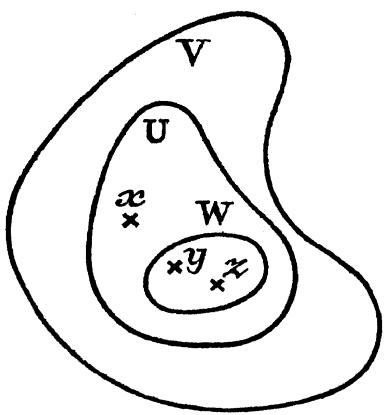
\includegraphics[keepaspectratio]{images/part001_56c83e78.jpg}}\\
图 1.

命题 2 表明，X 上的拓扑可以借助 X 的点的邻域所成之集 \(\mathfrak{B}(x)\) 来定义，只须它们满足公理 \((\mathrm{V}_{\mathrm{I}})\)、\((\mathrm{V}_{\mathrm{II}})\)、\((\mathrm{V}_{\mathrm{III}})\) 与 \((\mathrm{V}_{\mathrm{IV}})\)。

例。我们可以在有理数集合 \(\mathbf{Q}\) 上定义一个拓扑，其开集取为所有有界开区间的并；这些子集所成之集当然满足 \((\mathrm{O}_{\mathbf{I}})\)，而要看出它满足 \((\mathrm{O}_{\mathbf{II}})\)，只须注意：若两个开区间 \(]a, b[\) 与 \(]c, d[\) 的交不空，则它是区间 \(]\alpha, \beta[\)，其中 \(\alpha = \sup (a, c)\) 与 \(\beta = \inf (b, d)\)。对每个 \(x \in \mathbf{Q}\)，把邻域所成之集 \(\mathfrak{B}(x)\)（即 \(x\) 的邻域全体）定义为包含某个含 \(x\) 的开区间的子集全体，就得到同一个拓扑。把该拓扑赋予 \(\mathbf{Q}\) 所得到的拓扑空间称为有理直线（参见第四章，§ 1，第 2 目）。注意，在此空间中每个开区间都是开集。* 我们可以用同样的方式在实数集合 \(\mathbf{R}\) 上定义拓扑；赋有该拓扑的 \(\mathbf{R}\) 称为实直线（参见 § 2，习题 5 及第四章，§ 1，第 3 目）。*

\subsection{基本邻域系；拓扑基}

定义 5. 在拓扑空间 X 中，点 x（相应地，X 的子集 A）的基本邻域系是指 x（相应地，A）的邻域所成的任一集合 S，使得对 x（相应地，A）的每个邻域 V，存在邻域 W ∈ S 满足 W ⊂ V。

如果 \(\mathfrak{S}\) 是子集 \(A\)（\(X\) 的子集）的基本邻域系，则 \(\mathfrak{S}\) 中集合的每个有限交都包含 \(\mathfrak{S}\) 的某个集合。

例。1) 在离散空间（第 1 目）中，单独的集合 \(\{x\}\) 就构成点 \(x\) 的基本邻域系。

\begin{enumerate}
\def\labelenumi{\arabic{enumi})}
\setcounter{enumi}{1}
\tightlist
\item
  在有理直线 Q 上，包含点 x 的所有开区间所成之集是该点的一个基本邻域系。开区间 \(]x - 1/n, x + 1/n[\) 所成之集，以及闭区间 \([x - 1/n, x + 1/n]\) 所成之集亦然，其中 n 取遍所有整数 \textgreater0，或取遍由整数 \textgreater0 组成的任一严格递增无穷序列。* 对实直线有类似的结果。*
\end{enumerate}

定义 6. 拓扑空间 X 的拓扑的拓扑基是指 X 的开子集所成的任一集合 B，使得 X 的每个开子集都是属于 B 的集合之并。

命题 3. 如果 X 是拓扑空间，则 X 的开子集所成的集合 B 是 X 的拓扑的拓扑基的充分必要条件是：对每个 \(x \in X\)，由 \(V \in B\)（其中 \(x \in V\)）所成之集是 x 的基本邻域系。

显然该条件是必要的。反之，若该条件成立，则对任一开集 U 与任一 \(x \in U\)，存在开集 \(V_{x} \in B\) 使得 \(x \in V_{x} \subset U\)。于是诸集合 \(V_{x}\)（对 \(x \in U\)）之并等于 U。证毕。

例。1) 离散拓扑以 X 的由单独一点组成的子集所成之集为一个拓扑基。

\begin{enumerate}
\def\labelenumi{\arabic{enumi})}
\setcounter{enumi}{1}
\tightlist
\item
  有界开区间所成之集依定义是有理直线（第 2 目）的拓扑的一个拓扑基。* 同样，有界开区间所成之集是实直线的拓扑的一个拓扑基。*
\end{enumerate}

\subsection{闭集}

定义 7. 在拓扑空间 X 中，X 的开集的余集称为闭集。

取余集，可知公理 \((\mathbf{O}_{\mathbf{I}})\) 与 \((\mathbf{O}_{\mathbf{II}})\) 取下列形式：

\((\mathbf{O}_{\mathbf{I}}^{\prime})\) 闭集的任何交是闭集。

\((\mathbf{O}_{\mathrm{II}}^{\prime})\) 闭集的任何有限并是闭集。

空集与整个空间 X 都是闭集（从而既开又闭；参见 § 11）。

在有理直线上，每个形如 \([a, \rightarrow[\) 的区间都是闭集，因为它的余集 \(]\leftarrow, a[\) 是开集；同样，每个形如 \(]\leftarrow, a]\) 的区间都是闭集；从而每个有界闭区间 \([a, b]\) 也是闭集，因为它是区间 \([a, \rightarrow[\) 与 \(]\leftarrow, b]\) 之交。

有理整数集 Z 在有理直线中是闭集，因为它的

余集 \(\bigcup_{n\in \mathbf{Z}}]n,n + 1[\) 是开集。

设 \((\mathbf{F}_i)_{i\in I}\) 是 \(\mathbf{A}\)（拓扑空间 \(\mathbf{X}\) 的一个子集）的覆盖；如果每个 \(\mathbf{F}_i\) 在 \(\mathbf{X}\) 中都是闭集，则称该覆盖为闭覆盖。

同胚 \(f\)（由拓扑空间 \(\mathbf{X}\) 到拓扑空间 \(\mathbf{X}'\) 上，第 1 目）可以刻画为 \(\mathbf{X}\) 到 \(\mathbf{X}'\) 上的一个双射，使得在 \(f\) 之下，\(\mathbf{X}\) 的每个闭子集的像是 \(\mathbf{X}'\) 的闭子集，并且在 \(f\) 之下，\(\mathbf{X}'\) 的每个闭子集的逆像是 \(\mathbf{X}\) 的闭子集。

\subsection{局部有限族}

定义 8. 族 \((\mathbf{A}_{i})_{i\in \mathbf{I}}\)（拓扑空间 \(\mathbf{X}\) 的子集所成的族）称为局部有限的，如果对每个 \(x\in \mathbf{X}\)，存在一个邻域 \(\mathbf{V}\)（\(x\) 的邻域），使得 \(\mathbf{V}\cap \mathbf{A}_i = \emptyset\) 对除去有限多个指标 \(i\in \mathbf{I}\) 外成立。子集所成的集合 \(\mathfrak{S}\)（\(\mathbf{X}\) 的子集所成之集）称为局部有限的，如果由 \(\mathfrak{S}\) 到自身的恒等映射所定义的子集族是局部有限的。

显然，如果 \((\mathbf{A}_t)_{t \in \mathbf{I}}\) 是局部有限的子集族，并且 \(\mathbf{B}_t \subset \mathbf{A}_t\) 对每个 \(t \in \mathbf{I}\) 成立，则族 \((\mathbf{B}_t)_{t \in \mathbf{I}}\) 是局部有限的。

拓扑空间的每个有限子集族显然是局部有限的；反之一般不成立。

* 例如，在 R 中，由区间 \(]\leftarrow, 1[\) 与诸区间 \(]n, \rightarrow[\)（对每个整数 \(n\geqslant0\)）所形成的开覆盖是局部有限的；而每个区间 \(]n, \rightarrow[\) 都与该覆盖中的无穷多个集合相交。

命题 4. 拓扑空间 X 的闭子集所成的局部有限族之并在 X 中是闭集。

设 \((\mathbf{F}_i)_{i\in I}\) 是 \(X\) 的闭子集所成的一个局部有限族，并设 \(x\in X\) 不属于 \(\mathbf{F} = \bigcup_{i\in I}\mathbf{F}_i\)；则 \(x\) 有一个邻域 \(V\)，它只与那些 \(\mathbf{F}_i\) 相交，后者的指标属于某个有限子集 \(J\)（\(I\) 的子集）。对每个 \(i\in J\)，设 \(\mathbf{U}_i\) 为 \(\mathbf{F}_i\) 的余集；则 \(\mathbb{CF}\) 包含集合 \(V\cap \bigcap_{i\in J}\mathbf{U}_i\)，后者是 \(x\) 的一个邻域，因为每个 \(\mathbf{U}_i\) 都是开集且包含 \(x\)。于是，由第 2 目的命题 1，\(\mathbb{CF}\) 是开集，从而 \(\mathbf{F}\) 在 \(X\) 中是闭集。

我们注意到，X 的闭子集所成的任意族之并未必是闭集；例如，在有理直线 Q 上，集合 \(]0, 1[\) 是诸闭集

\[
\left[ \frac {1}{n}, 1 - \frac {1}{n} \right] \quad \text { for } n > 2,
\]

之并，但它不是闭集。

\subsection{集合的内部、闭包、边界；稠密集}

定义 9. 在拓扑空间 X 中，点 x 称为 X 的子集 A 的内点，如果 A 是 x 的邻域。A 的内点所成之集称为 A 的内部，记作 \(\mathring{A}\)。

根据定义 9 与定义 4，点 x 是 A 的内点，如果存在包含在 A 中且包含 x 的开集；由此可知 \(\mathring{A}\) 是包含在 A 中的所有开集之并，因而是包含在 A 中的最大开集：换言之，若 B 是包含在 A 中的开集，则 B ⊂ \(\mathring{A}\)。从而，若 A 与 B 是 X 的两个子集且 B ⊂ A，则 \(\mathring{B} \subset \mathring{A}\)；并且 A 是 B 的邻域当且仅当 B ⊂ \(\mathring{A}\)。

注. 非空集合的内部可以是空集；例如，由单独一点（该点不是开集）组成的集合就是这种情形，比如在有理直线上 * （或实直线上） *。

第 2 目的命题 1 可以改述如下：

一个集合是开集当且仅当它与自己的内部相重合。

第 2 目的性质 \((V_{II})\) 蕴含：凡是两个子集 A 与 B 中每一个的内点的点，都是 \(A \cap B\) 的内点；从而

\[
\mathring {\mathbf {A} \cap \mathbf {B}} = \mathring {\mathbf {A}} \cap \mathring {\mathbf {B}}.\tag{1}
\]

凡是集合 A 的余集的内点的点称为 A 的外点，这些点所成之集称为 A 在 X 中的外部；因此，点 \(x \in X\) 是 A 的外点这一事实可由下述性质刻画：x 有一个不与 A 相交的邻域。

定义 10. 拓扑空间 X 的子集 A 的闭包是指由所有这样的点 \(x \in X\) 组成的集合：x 的每个邻域都与 A 相交；闭包记作 \(\overline{A}\)。

这个定义可以改述为：点 x 位于集合 A 的闭包中，如果 A 中存在与 x 要多接近就有多接近的点。

凡不属于 A 的闭包的点都是 A 的外点，反之亦然；于是我们有下列（互为对偶的）公式

\[
\mathbf {C} \overline {{\mathbf {A}}} = \mathring {\mathbf {C} \mathbf {A}}, \quad \mathbf {C} \mathring {\mathbf {A}} = \overline {{\mathbf {C} \mathbf {A}}}.\tag{2}
\]

因此，由对偶性，关于集合内部的每个命题都对应一个关于闭包的命题，反之亦然。特别地，集合 A 的闭包是包含 A 的最小闭集；换言之，若 B 是使 \(A \subset B\) 成立的闭集，则 \(\overline{A} \subset B\)。若 A 与 B 是 X 的两个子集且 \(A \subset B\)，则 \(\overline{A} \subset \overline{B}\)。

一个集合是闭集当且仅当它与自己的闭包相重合。

公式 (1) 的对偶是

\[
\overline {{{\mathbf {A} \cup \mathbf {B}}}} = \overline {{{\mathbf {A}}}} \cup \overline {{{\mathbf {B}}}}.\tag{3}
\]

命题 5. 设 A 是 X 中的开集；则对 X 的每个子集 B，我们有

\[
\mathbf {A} \cap \overline {{\mathbf {B}}} \subset \overline {{\mathbf {A} \cap \mathbf {B}}}.\tag{4}
\]

因为设 \(x \in A \cap \overline{B}\)；则若 V 是 x 的任一邻域，\(V \cap A\) 是 x 的邻域（因 A 是开集）；于是 \(V \cap A \cap B\) 非空，从而 x 位于 \(A \cap B\) 的闭包中。

如果 \(x\) 位于 \(A\) 的闭包中但不属于 \(A\)，则 \(x\) 的每个邻域都包含 \(A\) 中一个异于 \(x\) 的点；但若 \(x \in A\)，则可能发生这样的情形：\(x\) 有一个邻域，它不含 \(A\) 的任何异于 \(x\) 的点。这时我们说 \(x\) 是 \(A\) 的孤立点。特别地，\(x\) 在整个空间 \(X\) 中是孤立点当且仅当 \(\{x\}\) 是开集。

没有孤立点的闭集称为完备集。

定义 11. 在拓扑空间 X 中，点 x 称为集合 A 的边界点，如果 x 既位于 A 的闭包中又位于 CA 的闭包中。A 的边界点所成之集称为 A 的边界。

于是 A 的边界是集合 \(\overline{A} \cap \overline{\complement A}\)，它是闭集。A 的边界点 x 可由下述性质刻画：x 的每个邻域至少包含 A 的一个点和 CA 的一个点；x 可以属于 A 也可以不属于 A。A 的边界与 CA 的边界相同。A 的内部、A 的外部与 A 的边界两两不相交，其并是整个空间 X。

定义 12. 拓扑空间 X 的子集 A 称为在 X 中稠密（若关于 X 不会引起混淆，就简称稠密），如果 \(\overline{A} = X\)，亦即如果 X 的每个非空开集 U 都与 A 相交。

例。* 我们将在第四章 § 1 中看到，有理数集及其余集在实直线上都稠密。*

在离散空间 X 中，X 的唯一稠密子集是 \(X^{*}\) 自身。另一方面，在 X 上以 \(\varnothing\) 与 X 为仅有开集的拓扑中，X 的每个非空子集都稠密。

命题 6. 如果 \(\mathfrak{B}\) 是拓扑空间 \(X\) 的拓扑的一个拓扑基，则存在一个稠密集 \(D\)（在 \(X\) 中），使得 \(\operatorname{Card}(D) \leqslant \operatorname{Card}(\mathfrak{B})\)。

我们可以限于 \(\mathfrak{B}\) 中没有集合是空集的情形（\(\mathfrak{B}\) 的非空集合已经构成 \(\mathbf{X}\) 的拓扑的一个拓扑基）。对每个 \(\mathbf{U} \in \mathfrak{B}\)，设 \(x_{\mathbf{U}}\) 是 \(\mathbf{U}\) 的一个点；由第 3 目的命题 3 可知，集合 \(\mathbf{D}\)（由诸点 \(x_{\mathbf{U}}\) 组成）在 \(\mathbf{X}\) 中稠密，并且我们有 Card \((\mathbf{D}) \leqslant\) Card \((\mathfrak{B})\)（《集合论》，第三章，§ 3，第 2 目，命题 3）。

\section{连续函数}

\subsection{连续函数}

定义 1. 映射 \(f\)（由拓扑空间 \(\mathbf{X}\) 到拓扑空间 \(\mathbf{X}'\) 中的映射）称为在点 \(x_0 \in \mathbf{X}\) 处连续，如果对任一邻域 \(\mathbf{V}'\)（\(f(x_0)\) 在 \(\mathbf{X}'\) 中的邻域），存在一个邻域 \(\mathbf{V}\)（\(x_0\) 在 \(\mathbf{X}\) 中的邻域），使得关系 \(x \in \mathbf{V}\) 蕴含 \(f(x) \in \mathbf{V}'\)。

定义 1 可以改述为下列更直观的形式：说 \(f\) 在点 \(x_0\) 处连续，意思是 \(f(x)\) 可以随意地接近 \(f(x_0)\)，只要 \(x\) 充分接近 \(x_0\)。

关系“对每个 \(x \in V\)，\(f(x) \in V'\)”等价于 \(f(V) \subset V'\)，或者再等价于 \(V \subset \overline{f}^{1}(V')\)；鉴于邻域公理 \((V_{I})\)，我们看到定义 1 等价于下述定义：称 \(f: X \to X'\) 在点 \(x_{0}\) 处连续，如果对每个邻域 \(V'\)（\(f(x_{0})\) 在 \(X'\) 中的邻域），\(\overline{f}^{1}(V')\) 是 \(x_{0}\) 在 X 中的邻域。而且，只需 \(\overline{f}^{1}(V')\) 是 \(x_{0}\) 的邻域（对每个邻域 \(V'\)，它属于 \(f(x_{0})\) 在 \(X'\) 中的某个基本邻域系）就够了（§ 1，第 3 目）。

命题 1. 设 \(f\) 是由拓扑空间 \(\mathbf{X}\) 到拓扑空间 \(\mathbf{X}'\) 中的一个映射。如果 \(f\) 在 \(x\) 处连续，并且 \(x\) 位于子集 \(A\)（\(X\) 的子集）的闭包中，则 \(f(x)\) 位于 \(f(A)\) 的闭包中。

设 \(\mathbf{V}'\) 是 \(f(x)\) 在 \(\mathbf{X}'\) 中的一个邻域。由于 \(f\) 在 \(x\) 处连续，\(\overline{f}^1 (\mathbf{V}')\) 是 \(x\) 在 \(\mathbf{X}\) 中的邻域。于是 \(\overline{f}^1 (\mathbf{V}')\) 与 \(\mathbf{A}\) 相交，由此推出 \(\mathbf{V}'\) 与 \(f(\mathbf{A})\) 相交，从而 \(f(x)\) 位于 \(f(\mathbf{A})\) 的闭包中。

命题 2. 设 X、X'、X'' 是三个拓扑空间；设 f 是由 X 到 X' 中的映射，在 x ∈ X 处连续；设 g 是由 X' 到 X'' 中的映射，在 f(x) 处连续。则复合映射 h = g \(\circ\) f: X → X'' 在 x 处连续。

设 \(V''\) 是 \(h(x) = g(f(x))\) 在 \(X''\) 中的一个邻域。由于 \(g\) 在 \(f(x)\) 处连续，可知 \(\overline{g}^1(V'')\) 是 \(f(x)\) 在 \(X'\) 中的邻域。但 \(f\) 在 \(x\) 处连续，故 \(\overline{f}^1(\overline{g}^1(V'')) = \overline{h}^1(V'')\) 是 \(x\) 在 \(X\) 中的邻域，从而 \(h\) 在 \(x\) 处连续。

定义 2. 由拓扑空间 X 到拓扑空间 X' 中的映射称为在 X 上连续（或简称连续），如果它在 X 的每一点都连续。

例。1) 拓扑空间 X 到自身的恒等映射是连续的。

\begin{enumerate}
\def\labelenumi{\arabic{enumi})}
\setcounter{enumi}{1}
\item
  拓扑空间到拓扑空间中的常映射是连续的。
\item
  由离散空间到拓扑空间中的每个映射都是连续的。
\end{enumerate}

定理 1. 设 \(f\) 是由拓扑空间 \(X\) 到拓扑空间 \(X'\) 中的一个映射。则下列命题等价：

\begin{enumerate}
\def\labelenumi{\alph{enumi})}
\item
  \(f\) 在 \(\mathbf{X}\) 中连续。
\item
  对 X 的每个子集 A，\(f(\overline{\mathrm{A}}) \subset \overline{f(\mathrm{A})}\)。
\item
  在 \(f\) 之下，\(\mathbf{X}'\) 的每个闭子集的逆像是 \(\mathbf{X}\) 的闭子集。
\item
  在 \(f\) 之下，\(\mathbf{X}'\) 的每个开子集的逆像是 \(\mathbf{X}\) 的开子集。
\end{enumerate}

我们已经看到 a) 蕴含 b)（命题 1）。为证 b) 蕴含 c)，设 \(\mathbf{F}'\) 是 \(\mathbf{X}'\) 的闭子集，并设 \(\mathbf{F} = \overline{f}^{1}(\mathbf{F}')\)；则由假设 \(f(\overline{\mathbf{F}}) \subset \overline{f(\mathbf{F})} \subset \overline{\mathbf{F}}' = \mathbf{F}'\)，故 \(\overline{\mathbf{F}} \subset \overline{f}^{1}(\mathbf{F}') = \mathbf{F} \subset \overline{\mathbf{F}}\)，于是 \(\mathbf{F} = \overline{\mathbf{F}}\)，即 \(\mathbf{F}\) 是闭集。鉴于关系式 \(\complement \overline{f}^{1}(A') = \overline{f}^{1}(\complement A')\)（对每个子集 \(A'\)（\(X'\) 的子集）成立），c) 蕴含 d)。最后，设 d) 成立。设 \(x\) 是 \(X\) 的任一点，并设 \(V'\) 是 \(f(x)\) 在 \(X'\) 中的任一邻域；则存在开集 \(A'\)（\(X'\) 中的），使得

\[
f (x) \in \mathrm{A} ^ {\prime} \subset \mathrm{V} ^ {\prime}
\]

从而 \(x \in \overline{f}^1(\mathbf{A}') \subset \overline{f}^1(\mathbf{V}')\)。由假设，\(\overline{f}^1(\mathbf{A}')\) 在 \(\mathbf{X}\) 中是开集，于是 \(\overline{f}^1(\mathbf{V}')\) 是 \(x\) 在 \(\mathbf{X}\) 中的邻域。这样 d) 蕴含 a)。

注。1) 设 \(\mathfrak{B}\) 是 \(\mathbf{X}'\) 的拓扑的一个拓扑基（§ 1，第 3 目）；则为使 \(f: \mathbf{X} \to \mathbf{X}'\) 连续，必要且充分的是：\(\overline{f}^1(\mathbf{U}')\) 在 \(\mathbf{X}\) 中是开集（对每个 \(\mathbf{U}' \in \mathfrak{B}\)）。

例。设 \(a\) 是任一有理数。映射 \(x \to a + x\)（由有理直线 \(\mathbf{Q}\) 到自身的映射）在 \(\mathbf{Q}\) 上连续，因为开区间 \(]b, c[\) 在该映射下的逆像是开区间

\[
] b - a, c - a [.
\]

同样，映射 \(x \to ax\) 在 \(\mathbf{Q}\) 上连续；若 \(a = 0\) 这是显然的，因为此时 \(ax = 0\) 对所有 \(x\) 成立；若 \(a \neq 0\)，则开区间 \(]b, c[\) 在该映射下的逆像是以 \(b / a\) 与 \(c / a\) 为端点的开区间。

\pandocbounded{
\includegraphics[keepaspectratio]{images/part001_4077020d.jpg}}

\begin{enumerate}
\def\labelenumi{\arabic{enumi})}
\setcounter{enumi}{1}
\tightlist
\item
  在连续映射 \(f: \mathbf{X} \to \mathbf{X}'\) 下，X 的开（相应地，闭）集的直接像在 \(\mathbf{X}'\) 中未必是开（相应地，闭）集（参见 § 5）。
\end{enumerate}

例。* 映射 \(f: x \to 1 / (1 + x^2)\)（由 \(\mathbf{R}\) 到自身的映射）是连续的，但 \(f(\mathbf{R})\) 是半开区间 {[}0, 1{]}，它在 \(\mathbf{R}\) 中既不是开集也不是闭集。*

定理 2. 1) 如果 \(f: \mathbf{X} \to \mathbf{X}'\) 与 \(g: \mathbf{X}' \to \mathbf{X}''\) 是两个连续映射，则 \(g \circ f: \mathbf{X} \to \mathbf{X}''\) 连续。

\begin{enumerate}
\def\labelenumi{\arabic{enumi})}
\setcounter{enumi}{1}
\tightlist
\item
  为使双射 \(f\)（由拓扑空间 \(X\) 到拓扑空间 \(X'\) 上的双射）是同胚，必要且充分的是 \(f\) 与 \(f\) 的逆都连续（或者说，\(f\) 是双连续的）。
\end{enumerate}

第一个断言是命题 2 的直接推论；第二个断言由定理 1 的 d) 与同胚的定义（§ 1，第 1 目）得出。

\pandocbounded{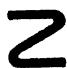
\includegraphics[keepaspectratio]{images/part001_720050f1.jpg}}

注。1) 可能存在由拓扑空间 X 到拓扑空间 X' 上的连续双射而不是双连续的：例如，取 X' 为有理直线 Q，取 X 为赋予离散拓扑的集合 Q；则恒等映射 X → X' 连续但不是同胚。

\begin{enumerate}
\def\labelenumi{\arabic{enumi})}
\setcounter{enumi}{1}
\item
  为验证连续双射 \(f: \mathbf{X} \to \mathbf{X}'\) 是同胚，只需证明：对每个 \(x \in \mathbf{X}\) 与每个邻域 \(V\)（\(x\) 的邻域），\(f(V)\) 是 \(f(x)\) 在 \(\mathbf{X}'\) 中的邻域。
\item
  设 X 是拓扑空间，对每个 \(x \in X\)，设 \(\mathfrak{B}(x)\) 是 x 的所有邻域所成之集。设 \(x_{0}\) 是 X 的一点；对每个 \(x \in X\)，按如下方式定义 X 的子集所成之集 \(\mathfrak{B}_{0}(x)\)：\(\mathfrak{B}_{0}(x_{0}) = \mathfrak{B}(x_{0})\)，而若 \(x \neq x_{0}\)，则 \(\mathfrak{B}_{0}(x)\) 取为 X 的包含 x 的所有子集所成之集。立即可以验证（§ 1，第 2 目，命题 2），诸集 \(\mathfrak{B}_{0}(x)\) 是 X 上某个拓扑的诸点的邻域集；用 \(X_{0}\) 表示这样得到的拓扑空间，用 \(j : X_{0} \to X\) 表示恒等映射，它连续但一般不是双连续的。X 到拓扑空间 \(X'\) 中的映射 f 在点 \(x_{0}\) 处连续当且仅当复合映射 \(X_{0} \stackrel{j}{\to} X \stackrel{f}{\to} X'\) 在 \(X_{0}\) 上连续；这由定义立即得出。
\end{enumerate}

\subsection{拓扑的比较}

第 1 目的定理 2 表明，我们可以把连续映射取作拓扑结构的态射（《集合论》，第四章，§ 2，第 1 目）；从现在起，我们假定已作出了这样的态射选取。按照一般定义（《集合论》，第四章，§ 2，第 2 目），这使我们可以对给定集合 X 上的诸拓扑所成之集定义一个序：

定义 3. 给定同一集合 X 上的两个拓扑 \(\mathfrak{C}_1\)、\(\mathfrak{C}_2\)，我们说 \(\mathfrak{C}_1\) 比 \(\mathfrak{C}_2\) 细（而 \(\mathfrak{C}_2\) 比 \(\mathfrak{C}_1\) 粗），如果记 \(X_i\) 为赋以拓扑 \(\mathfrak{C}_i\)（\(i = 1, 2\)）的集合 X，恒等映射 \(X_1 \to X_2\) 连续。若此外还有 \(\mathfrak{C}_1 \neq \mathfrak{C}_2\)，则说 \(\mathfrak{C}_1\) 比 \(\mathfrak{C}_2\) 严格地细（而 \(\mathfrak{C}_2\) 比 \(\mathfrak{C}_1\) 严格地粗）。

两个拓扑，若其中一个比另一个细，则称它们是可比较的。

映射连续性的判别法（第 1 目，定义 1 与定理 1）给出下列命题：

命题 3. 给定两个拓扑 \(\mathfrak{G}_1\)、\(\mathfrak{G}_2\)（集合 \(X\) 上的拓扑），下列命题等价：

\begin{enumerate}
\def\labelenumi{\alph{enumi})}
\item
  \(\mathfrak{C}_1\) 比 \(\mathfrak{C}_2\) 细。
\item
  对每个 \(x \in \mathbf{X}\)，\(x\) 关于 \(\mathfrak{C}_2\) 的每个邻域都是 \(x\) 关于 \(\mathfrak{C}_1\) 的邻域。
\item
  对 X 的每个子集 A，A 在拓扑 \(C_{1}\) 中的闭包包含在 A 在拓扑 \(C_{2}\) 中的闭包之中。
\item
  在 \(\mathfrak{C}_{2}\) 中为闭集的 X 的每个子集在 \(\mathfrak{C}_{1}\) 中也是闭集。
\item
  在 \(\mathfrak{C}_{2}\) 中为开集的 X 的每个子集在 \(\mathfrak{C}_{1}\) 中也是开集。
\end{enumerate}

例。* 在由实数的序列 \(x = (x_n)\) 组成的 Hilbert 空间 H 中，这些序列满足

\[
\| x \| ^ {2} = \sum_ {n = 0} ^ {\infty} x _ {n} ^ {2} <   + \infty ,
\]

点 \(x_0\) 在 H 上的强拓扑中的邻域是包含开球 \(\|x - x_0\| < a\)（以 \(x_0\) 为中心的开球）的集合；\(x_0\) 在 H 上的弱拓扑中的邻域是包含由形如 \(\sup_{1 \leqslant i \leqslant n} |(x - x_0|a_i)| \leqslant 1\) 的关系所定义之集的集合，其中诸 \(a_i\) 是 H 的点，并且

\[
(x | y) = \sum_ {n = 0} ^ {\infty} x _ {n} y _ {n}
\]

（若 \(x = (x_n)\) 且 \(y = (y_n)\)）。现在若 \(\beta = \sup_{1 \leqslant i \leqslant n} \|a_i\|\)，则关系 \(\|x - x_0\| \leqslant 1/\beta\) 蕴含 \(|(x - x_0|a_i)| \leqslant \|x - x_0\| \cdot \|a_i\| \leqslant 1\)（对 \(1 \leqslant i \leqslant n\)）；因此 H 上的强拓扑比弱拓扑细。另一方面，对 H 的点的任意有限族 \((a_i)_{1 \leqslant i \leqslant n}\)，存在 H 中的点 \(x\)，使 \((x - x_0|a_i) = 0\)（对 \(1 \leqslant i \leqslant n\)）且使 \(\|x - x_0\|\) 任意大；这表明强拓扑比弱拓扑严格地细。*

注。1) 在集合 X 上所有拓扑组成的有序集中，仅以 \(\varnothing\) 与 X 为开集的拓扑是最粗的，而离散拓扑是最细的。

\begin{enumerate}
\def\labelenumi{\arabic{enumi})}
\setcounter{enumi}{1}
\item
  拓扑越细，开集、闭集与邻域就越多；拓扑越细，集合的闭包（相应地，内部）就越小（相应地，越大）；拓扑越细，稠密集就越少。
\item
  如果 \(f: \mathbf{X} \to \mathbf{X}'\) 是连续映射，那么当把 \(\mathbf{X}\) 的拓扑换成较细的拓扑、把 \(\mathbf{X}'\) 的拓扑换成较粗的拓扑时，它仍然连续（第 1 目，定理 2）。换言之，\(\mathbf{X}\) 的拓扑越细且 \(\mathbf{X}'\) 的拓扑越粗，由 \(\mathbf{X}\) 到 \(\mathbf{X}'\) 中的连续映射就越多。
\end{enumerate}

\subsection{初始拓扑}

命题 4. 设 X 是一个集合，设 \((\mathbf{Y}_i)_{i \in I}\) 是拓扑空间的一个族，并且对每个 \(i \in I\)，设 \(f_i\) 是由 X 到 \(\mathbf{Y}_i\) 中的一个映射。设 \(\mathfrak{S}\) 是 X 的形如 \(\overline{f}_i^1 (\mathbf{U}_i)\)（\(i \in I\)，\(\mathbf{U}_i\) 在 \(\mathbf{Y}_i\) 中开）的子集所成之集，并设 \(\mathfrak{B}\) 是 \(\mathfrak{S}\) 的集合的有限交所成之集。则 \(\mathfrak{B}\) 是 X 上某个拓扑 \(\mathfrak{C}\) 的拓扑基，该拓扑是 X 关于族 \((f_i)\) 的初始拓扑结构（《集合论》，第四章，§ 2，第 3 目），特别地，它是使诸映射 \(f_i\) 连续的 X 上最粗的拓扑。更精确地说，若 \(g\) 是由拓扑空间 Z 到 X 中的映射，则 \(g\) 在某点 \(z \in Z\) 处连续（X 赋以拓扑 \(\mathfrak{C}\)）当且仅当每个函数 \(f_i \circ g\) 都在 \(z\) 处连续。

设 \(\mathfrak{D}\) 是属于 \(\mathfrak{B}\) 的集合的所有并所成之集；显然 \(\mathfrak{D}\) 满足公理 \((\mathrm{O}_{\mathrm{I}})\)，因为取并的运算是可结合的；而 \(\mathfrak{D}\) 满足公理 \((\mathrm{O}_{\mathrm{II}})\)，这是由于 \(\mathfrak{B}\) 的定义以及有限交对任意并的分配律 {[}Set Theory, R § 4, formula (37){]}。于是集合 \(\mathfrak{D}\) 是 X 关于某个拓扑 \(\mathfrak{G}\) 的开子集所成之集，\(\mathfrak{B}\) 是该拓扑的一个拓扑基。我们将证明命题的最后一个断言，由初始结构的一般性质（《集合论》，第四章，§ 2，第 3 目，判别准则 CST 9），它蕴含其余断言。首先，\(\mathfrak{S}\) 的定义表明诸 \(f_{i}\) 在 X 上连续（第 1 目，定理 1）；因此，若 \(g\) 在 \(z\) 处连续，则诸映射 \(f_{i} \circ g\) 亦然（第 1 目，命题 2）。反之，设所有映射 \(f_{i} \circ g\) 都在 \(z\) 处连续，并设 V 是 \(g(z)\) 在 X 中的一个邻域；按定义，存在 I 的一个有限子集 J，并且对每个 \(i \in J\)，存在开子集 \(\mathrm{U}_{i}\)（\(\mathrm{Y}_{i}\) 的开子集），使得 V 包含集合 \(\bigcap_{i \in J} f_{i}^{1}(\mathrm{U}_{i})\) 且 \(g(z)\) 属于这个集合。由此推出

\[
\overline {{g}} ^ {1} (\mathrm{V}) \supset \bigcap_ {i \in J} \overline {{g}} ^ {1} (\overline {{f}} _ {i} ^ {1} (\mathrm{U} _ {i})),
\]

而假设蕴含诸集合 \(\overline{g}^{1}(\overline{f}_{i}^{1}(\mathbf{U}_{i}))\) 中的每一个都是 \(z\) 在 \(\mathbf{Z}\) 中的邻域；于是 \(\overline{g}^{1}(\mathbf{V})\) 也是 \(z\) 在 \(\mathbf{Z}\) 中的邻域。证毕。

设 \(\mathfrak{B}_i\) 是 \(\mathbf{Y}_i(t\in I)\) 的拓扑的一个拓扑基；用 \(\mathfrak{S}'\) 表示 \(X\) 的形如 \(\overline{f}_i^1 (U_i)\) 的子集所成之集（对 \(t\in I\) 且 \(U_{t}\in \mathfrak{B}_{t}\)（对每个 \(t\in I\)））；若 \(\mathfrak{B}'\) 是 \(\mathfrak{S}'\) 的集合的有限交所成之集，则显然 \(\mathfrak{B}'\) 是拓扑 \(\mathfrak{C}\) 的一个拓扑基。

初始结构的一般性质（《集合论》，第四章，§ 2，第 3 目，判别准则 CST 10）特别地蕴含下列传递性质（其直接证明是十分容易的）：

命题 5. 设 X 是一个集合，\((Z_{t})_{t\in I}\) 是拓扑空间的一个族，\((J_{\lambda})_{\lambda\in L}\) 是 I 的一个分拆，而 \((Y_{\lambda})_{\lambda\in L}\) 是以 L 为指标的一族集合。又对每个 \(\lambda\in L\)，设 \(h_{\lambda}\) 是由 X 到 \(Y_{\lambda}\) 中的一个映射；对每个 \(\lambda\in L\) 与每个 \(t\in J_{\lambda}\)，设 \(g_{t\lambda}\) 是由 \(Y_{\lambda}\) 到 \(Z_{t}\) 中的一个映射，并令 \(f_{t}=g_{t\lambda}\circ h_{\lambda}\)。如果每个 \(Y_{\lambda}\) 都赋以使诸映射 \(g_{t\lambda}(t\in J_{\lambda})\) 连续的最粗拓扑，那么使诸 \(f_{t}\) 连续的 X 上最粗的拓扑与使诸 \(h_{\lambda}\) 连续的最粗拓扑相同。

例。1) 拓扑的逆像。设 X 是一个集合，Y 是拓扑空间，f 是由 X 到 Y 中的映射；使 f 连续的 X 上最粗的拓扑 C 称为 Y 的拓扑在 f 下的逆像。由命题 4 以及并与交的逆像公式 {[}Set Theory, R, § 4, formulae (34) and (46){]} 可知，拓扑 C 中的开（相应地，闭）集是 Y 的开（相应地，闭）集在 f 下的逆像；从而，对每个 \(x \in X\)，诸集合 \(\overline{f}^{1}(W)\)（其中 W 取遍 \(f(x)\) 在 Y 中的某个基本邻域系）构成 x 在拓扑 C 中的基本邻域系。在 § 3 中我们将以诱导拓扑之名研究 X 是 Y 的子集且 f 是典范单射 \(X \to Y\) 这一特殊情形；这时赋以诱导拓扑的 X 称为 Y 的子空间。

为使映射 \(f\)（由拓扑空间 \(\mathbf{X}\) 到拓扑空间 \(\mathbf{X}'\) 中的映射）连续，必要且充分的是 \(\mathbf{X}\) 的拓扑比 \(f\) 之下 \(\mathbf{X}'\) 的拓扑的逆像细。

\begin{enumerate}
\def\labelenumi{\arabic{enumi})}
\setcounter{enumi}{1}
\tightlist
\item
  拓扑集的上确界。拓扑的每个族 \((\mathcal{C}_t)_{i\in I}\)（集合 \(X\) 上的拓扑的族）都有一个上确界 \(\mathcal{C}\)（在 \(X\) 上所有拓扑的有序集中），即存在 \(X\) 上的一个拓扑，它在 \(X\) 上比每个 \(\mathcal{C}_t\) 都细的所有拓扑中是最粗的。为看出这一点，可以应用命题 4，取 \(Y_t\) 为集合 \(X\)（赋以拓扑 \(\mathcal{C}_t\)），取 \(f_t\) 为恒等映射 \(X\to Y_t\)；\(\mathcal{C}\) 是使所有映射 \(f_t\) 连续的最粗拓扑。
\end{enumerate}

设 \(\mathfrak{S}\) 是集合 X 的子集的任意集合；在 X 上的诸拓扑 \(\mathfrak{C}\)（使 \(\mathfrak{S}\) 的集合皆为开集者）中，有一个拓扑 \(\mathfrak{C}_0\) 比其他所有拓扑都粗，称为由 \(\mathfrak{S}\) 生成的拓扑。对每个集合 \(U \in \mathfrak{S}\)，设 \(\mathfrak{C}_U\) 为以 \(\varnothing\)、U 与 X 为开集的拓扑{[}显然 X 的这个子集集合满足 \((O_I)\) 与 \((O_{II})]\)；则 \(\mathfrak{C}_0\) 恰是诸拓扑 \(\mathfrak{C}_U\) 的上确界。由命题 4，若 \(\mathfrak{B}\) 是属于 \(\mathfrak{S}\) 的集合的有限交所成之集，则 \(\mathfrak{B}\) 是拓扑 \(\mathfrak{C}_0\) 的一个拓扑基。我们说 \(\mathfrak{S}\) 是 \(\mathfrak{C}_0\) 的一个子基。

\begin{enumerate}
\def\labelenumi{\arabic{enumi})}
\setcounter{enumi}{2}
\tightlist
\item
  积拓扑。设 \((\mathbf{X}_t)_{i \in I}\) 是拓扑空间的一个族。积集合 \(\mathbf{X} = \prod_{i \in I} \mathbf{X}_i\) 上使诸
\end{enumerate}

投影 \(pr_{i}: X \rightarrow X_{i}\) 为连续映射的最粗拓扑称为诸 \(X_{i}\) 的拓扑之积；我们将在 § 4 中更详细地研究它。

\subsection{终拓扑}

命题 6. 设 X 是一个集合，设 \((\mathbf{Y}_t)_{t \in I}\) 是拓扑空间的一个族，并且对每个 \(t \in I\)，设 \(f_t\) 是由 \(\mathbf{Y}_t\) 到 X 中的映射。设 \(\mathfrak{D}\) 是 X 的这样的子集 U 所成之集：\(\overline{f}_t^1(\mathbf{U})\) 在 \(\mathbf{Y}_t\) 中是开集（对每个 \(t \in I\)）；则 \(\mathfrak{D}\) 是 X 上某个拓扑 \(\mathfrak{C}\) 的开子集所成之集，该拓扑是 X 关于族 \((f_t)\) 的终结构（《集合论》，第四章，§ 2，第 5 目），特别地，\(\mathfrak{C}\) 是使诸映射 \(f_t\) 连续的 X 上最细的拓扑。换言之，若 g 是由 X 到拓扑空间 Z 中的映射，则 g 连续（X 赋以拓扑 \(\mathfrak{C}\)）当且仅当每个映射 \(g \circ f_t\) 连续。

立即可以验证 \(\mathfrak{D}\) 满足公理 \((\mathrm{O_I})\) 与 \((\mathrm{O_{II}})\)。{[}Set Theory, R, § 4, formulae (34) and (46){]}。我们将证明命题的最后一个断言，由终结构的一般性质（《集合论》，第四章，§ 2，第 5 目，判别准则 CST 18），它蕴含其余断言。显然诸 \(f_{i}\) 在拓扑 \(\mathfrak{C}\) 中连续，这由 \(\mathfrak{D}\) 的定义得出（第 1 目，定理 1）；因此若 \(g\) 连续，则每个映射 \(g \circ f_{i}\) 连续（第 1 目，定理 2）。反之，设每个 \(g \circ f_{i}\) 都连续，并设 V 是 Z 中的开集；由假设，\(\overline{f}_{i}^{1}(\overline{g}^{1}(V))\) 在 \(Y_{i}\) 中是开集（对每个 \(i \in I\)）；于是 \(\overline{g}^{1}(V) \in \mathfrak{D}\)，证明完成。

推论. 在命题 6 的假设下，X 的子集 F 在拓扑 \(\mathfrak{C}\) 中是闭集当且仅当 \(\overline{f}_{\iota}^{1}(\mathbf{F})\) 在 \(Y_{\iota}\) 中是闭集（对每个 \(\iota \in I\)）。这由拓扑 \(\mathfrak{C}\) 中开集的定义取余集得出。

终结构的一般性质（《集合论》，第四章，§ 2，第 5 目，判别准则 CST 19）蕴含下列传递性质（其直接证明同样是容易的）：

命题 7. 设 X 是一个集合，\((Z_{\iota})_{\iota \in I}\) 是拓扑空间的一个族，\((J_{\lambda})_{\lambda \in L}\) 是 I 的一个分拆，而 \((Y_{\lambda})_{\lambda \in L}\) 是以 L 为指标的一族集合。又对每个 \(\lambda \in L\)，设 \(h_{\lambda}\) 是由 \(Y_{\lambda}\) 到 X 中的一个映射；对每个 \(\lambda \in L\) 与每个 \(\iota \in J_{\lambda}\)，设 \(g_{\lambda \iota}\) 是由 \(Z_{\iota}\) 到 \(Y_{\lambda}\) 中的一个映射，并令 \(f_{\iota} = h_{\lambda} \circ g_{\lambda \iota}\)。如果每个 \(Y_{\lambda}\) 都赋以使诸映射 \(g_{\lambda \iota} (\iota \in J_{\lambda})\) 连续的最细拓扑，那么使诸 \(f_{\iota}\) 连续的 X 上最细的拓扑与使诸 \(h_{\lambda}\) 连续的最细拓扑相同。

\paragraph*{例}

\begin{enumerate}
\def\labelenumi{\arabic{enumi})}
\item
  商拓扑。设 X 是拓扑空间，R 是 X 上的一个等价关系，Y = X/R 是 X 关于关系 R 的商集，\(\varphi: X \to Y\) 是典范映射。使 \(\varphi\) 连续的 Y 上最细的拓扑称为 X 的拓扑被关系 R 的商；我们将在 § 3 中更详细地研究它。
\item
  拓扑集的下确界。拓扑的每个族 \((\mathfrak{C}_t)_{i \in I}\)（集合 \(X\) 上的拓扑的族）都有一个下确界 \(\mathfrak{C}\)（在 \(X\) 上所有拓扑的集合中），即 \(\mathfrak{C}\) 是 \(X\) 上比每个 \(\mathfrak{C}_t\) 都粗的所有拓扑中最细的一个。为看出这一点，可以应用命题 6，取 \(Y_t\) 为集合 \(X\)（赋以拓扑 \(\mathfrak{C}_t\)），取 \(f_t\) 为恒等映射 \(Y_t \to X\)。若 \(\mathfrak{D}_t\) 是 \(X\) 的在拓扑 \(\mathfrak{C}_t\) 中为开集的子集所成之集，则集合 \(\bigcap_{i \in I} \mathfrak{D}_t\) 是 \(X\) 的在 \(\mathfrak{C}\) 中为开集的子集所成之集。
\end{enumerate}

\(\mathfrak{G}\) 也称为诸拓扑 \(\mathfrak{G}_{t}\) 的交。

\begin{enumerate}
\def\labelenumi{\arabic{enumi})}
\setcounter{enumi}{2}
\tightlist
\item
  拓扑空间的和。设 \((\mathbf{X}_t)_{i \in I}\) 是拓扑空间的一个族，\(\mathbf{X}\) 是诸 \(\mathbf{X}_t\) 的和所成的集合（《集合论》，第二章，§ 4，第 8 目，定义 8）；对每个 \(i \in I\)，设 \(j_t\) 是由 \(\mathbf{X}_t\) 到 \(\mathbf{X}\) 中的典范（单射）映射。最细拓扑 \(\mathfrak{G}\)（\(\mathbf{X}\) 上的、使诸映射 \(j_t\) 连续者）称为诸 \(\mathbf{X}_t\) 的拓扑之和，而 \(\mathbf{X}\) 赋以这个拓扑后称为诸拓扑空间 \(\mathbf{X}_t\) 的和。让我们把每个 \(\mathbf{X}_t\) 与 \(\mathbf{X}\) 的一个子集借助 \(j_t\) 等同起来；则集合 \(\mathbf{A} \subset \mathbf{X}\) 在拓扑 \(\mathfrak{G}\) 中是开（相应地，闭）集当且仅当诸集合 \(\mathbf{A} \cap \mathbf{X}_t\) 中的每一个在 \(\mathbf{X}_t\) 中都是开（相应地，闭）集。特别地，诸 \(\mathbf{X}_t\) 中的每一个都既开又闭。
\end{enumerate}

下列命题推广了例 3 的情形：

命题 8. 设 X 是一个集合，\((\mathbf{X}_{\lambda})_{\lambda \in \mathbf{L}}\) 是 X 的子集的一个族。假设每个 \(X_{\lambda}\) 都赋有一个拓扑 \(C_{\lambda}\)，使得对每对指标 \((\lambda, \mu)\)：

\begin{enumerate}
\def\labelenumi{\arabic{enumi})}
\item
  \(\mathbf{X}_{\lambda} \cap \mathbf{X}_{\mu}\) 在拓扑 \(\mathfrak{C}_{\lambda}, \mathfrak{C}_{\mu}\) 的每一个中都是开（相应地，闭）集。
\item
  在 \(\mathbf{X}_{\lambda} \cap \mathbf{X}_{\mu}\) 上由 \(\mathfrak{C}_{\lambda}\) 与 \(\mathfrak{C}_{\mu}\) 诱导的拓扑相重合。设 \(\mathfrak{C}\) 是 \(\mathbf{X}\) 上使诸单射 \(j_{\lambda}: \mathbf{X}_{\lambda} \to \mathbf{X}\) 连续的最细拓扑。则对每个 \(\lambda \in \mathbf{L}\)，\(\mathbf{X}_{\lambda}\) 在 \(\mathbf{X}\) 中在拓扑 \(\mathfrak{C}\) 下是开（相应地，闭）集，并且 \(\mathfrak{C}\) 在 \(\mathbf{X}_{\lambda}\) 上诱导的拓扑与 \(\mathfrak{C}_{\lambda}\) 相重合。
\end{enumerate}

鉴于命题 6 及其推论，只需证明：对每个 \(\lambda\) 与每个子集 \(A_{\lambda}\)（\(X_{\lambda}\) 的子集），下列命题等价：

\begin{enumerate}
\def\labelenumi{(\roman{enumi})}
\item
  \(\mathbf{A}_{\lambda}\) 在拓扑 \(\mathfrak{C}_{\lambda}\) 中是开（相应地，闭）集。
\item
  对每个 \(\mu \in L\)，\(A_{\lambda} \cap X_{\mu}\) 在拓扑 \(\mathfrak{G}_{\mu}\) 中是开（相应地，闭）集。
\end{enumerate}

显然，取 \(\mu = \lambda\) 即可看出 (ii) 蕴含 (i)。反之，若 (i) 成立，则 \(A_{\lambda} \cap X_{\mu}\) 在 \(X_{\lambda} \cap X_{\mu}\) 中相对于拓扑 \(\mathcal{C}_{\lambda\mu}\) 是开（相应地，闭）集；该拓扑在 \(X_{\lambda} \cap X_{\mu}\) 上由 \(\mathcal{C}_{\lambda}\) 诱导；但 \(\mathcal{C}_{\lambda\mu}\) 也是在 \(X_{\lambda} \cap X_{\mu}\) 上由 \(\mathcal{C}_{\mu}\) 诱导的拓扑；因此 \(A_{\lambda} \cap X_{\mu}\) 也是 \(X_{\lambda} \cap X_{\mu}\) 与一个子集 \(B_{\mu}\) 的交，其中该子集是 \(X_{\mu}\) 的子集且在拓扑 \(\mathcal{C}_{\mu}\) 中是开（相应地，闭）集；由于 \(X_{\lambda} \cap X_{\mu}\) 在 \(\mathcal{C}_{\mu}\) 中是开（相应地，闭）集，\(A_{\lambda} \cap X_{\mu}\) 也如此。证明完毕。

注意，若诸 \(\mathbf{X}_{\lambda}\) 的并不同于 \(\mathbf{X}\)，则 \(\mathcal{G}\) 在 \(\mathbf{X} - \left(\bigcup_{\lambda \in \mathbf{L}} \mathbf{X}_{\lambda}\right)\) 上诱导的拓扑是离散的。这是因为，若 \(x \in \mathbf{X}\) 不属于诸 \(\mathbf{X}_{\lambda}\) 中的任何一个，则 \(\{x\} \cap \mathbf{X}_{\lambda} = \emptyset\) 在每个拓扑 \(\mathcal{G}_{\lambda}\) 中都是开集，因而 \(\{x\}\) 在拓扑 \(\mathcal{G}\) 中是开集。

\subsection{拓扑空间的粘合}

设 \((\mathbf{X}_{\lambda})_{\lambda \in L}\) 是一个集合族，且设 \(\mathbf{X}\) 为作为诸 \(\mathbf{X}_{\lambda}\) 之和的那个集合（《集合论》第二章，§ 4，第 8 目，定义 8）；我们将把每个 \(\mathbf{X}_{\lambda}\) 与 \(\mathbf{X}\) 的一个子集（借助典范单射 \(j_{\lambda}: \mathbf{X}_{\lambda} \to \mathbf{X}\)）等同起来。

设 R 是 X 上的一个等价关系，使得 R 的每个等价类在每个 \(X_{\lambda}\) 中至多有一个元素；对每对指标 \((\lambda, \mu)\)，设 \(A_{\lambda\mu}\) 为 \(X_{\lambda}\) 的由这样的元素 x（存在属于 x 的等价类的元素 \(y \in X_{\mu}\)）组成的子集。显然，对每个 \(x \in A_{\lambda\mu}\)，对应着唯一的与 x 模 R 同余的 \(y \in A_{\mu\lambda}\)；如此定义的映射 \(h_{\mu\lambda}: A_{\lambda\mu} \to A_{\mu\lambda}\) 满足下列条件：

\begin{enumerate}
\def\labelenumi{(\roman{enumi})}
\item
  对每个 \(\lambda \in L\)，\(h_{\lambda \lambda}\) 是 \(\mathbf{A}_{\lambda \lambda} = \mathbf{X}_{\lambda}\) 上的恒等映射。
\item
  对指标的三元组 \((\lambda, \mu, \nu)\)（\(\mathbf{L}\) 中的三元组）以及每个 \(x \in \mathbf{A}_{\lambda \mu} \cap \mathbf{A}_{\lambda \nu}\)，我们有 \(h_{\mu \lambda}(x) \in \mathbf{A}_{\mu \nu}\)，并且
\end{enumerate}

\[
h _ {\nu \lambda} (x) = h _ {\nu \mu} (h _ {\mu \lambda} (x)).\tag{1}
\]

反之，假设对每对指标 \((\lambda, \mu)\) 给定了一个子集 \(A_{\lambda \mu}\)（\(X_{\lambda}\) 的子集）和一个满足上述条件 (i) 与 (ii) 的映射 \(h_{\mu \lambda}: A_{\lambda \mu} \to A_{\mu \lambda}\)。首先，把 (ii) 应用于三元组 \((\lambda, \mu, \lambda)\) 与 \((\mu, \lambda, \mu)\) 可知，\(h_{\lambda \mu} \circ h_{\mu \lambda}\)（相应地，\(h_{\mu \lambda} \circ h_{\lambda \mu}\)）是 \(h_{\lambda \lambda}\)（相应地，\(h_{\mu \mu}\)）在 \(A_{\lambda \mu}\)（相应地，\(A_{\mu \lambda}\)）上的限制；于是由 (i) 推出，\(h_{\lambda \mu}\) 与 \(h_{\mu \lambda}\) 是互为逆映射的双射。现在设 \(R\{x, y\}\) 是关系"存在 \(\lambda, \mu\) 使得 \(x \in A_{\lambda \mu}, y \in A_{\mu \lambda}\) 且 \(y = h_{\mu \lambda}(x)\)"。由 (i) 以及前文可知 \(R\) 是自反的且对称的；另一方面，若 \(x \in A_{\lambda \mu}\)，

\[
y = h _ {\mu \lambda} (x) \in A _ {\mu \lambda} \cap A _ {\mu \nu} \quad \text { and } \quad z = h _ {\nu \mu} (y),
\]

则也有 \(x = h_{\lambda \mu}(y)\)，从而由 (ii) 得 \(x \in A_{\lambda \mu} \cap A_{\lambda \nu}\)；于是关系式 (1) 表明 \(R\) 是传递的，因此 \(R\) 是 \(X\) 上的一个等价关系。由 (i) 以及 \(R\) 的定义还可得出：模 \(R\) 的每个等价类在诸集合 \(X_{\lambda}\) 的每一个中至多有一个元素，并且 \(A_{\lambda \mu}\) 是由所有这样的 \(x \in X_{\lambda}\)（存在元素 \(y \in X_{\mu}\) 与 \(x \mod R\) 同余）组成的集合。我们说，商集 \(X / R\) 是把诸 \(X_{\lambda}\) 沿 \(A_{\lambda \mu}\) 借助诸双射 \(h_{\mu \lambda}\) 粘合在一起而得到的。若 \(\varphi: X \to X / R\) 是典范映射，则 \(\varphi\) 在每个 \(X_{\lambda}\) 上的限制是由 \(X_{\lambda}\) 到 \(\varphi(X_{\lambda})\) 上的一个双射。

现在假设每个 \(X_{\lambda}\) 都是拓扑空间，并设 \(G_{\lambda}\) 为它的拓扑。设 G 为集合 X/R 上使诸映射 \(\varphi \circ j_{\lambda}\) 连续的最细拓扑；G 是 X 上作为诸拓扑 \(G_{\lambda}\) 之和的那个拓扑经 R 得到的商。我们说，拓扑空间 X/R（带拓扑 G）是把诸拓扑空间 \(X_{\lambda}\) 沿 \(A_{\lambda\mu}\) 借助诸双射 \(h_{\mu\lambda}\) 粘合在一起而得到的。于是，X/R 的开（相应地，闭）子集是 X 的子集 B（关于 R 饱和，且 \(B \cap X_{\lambda}\) 在 \(X_{\lambda}\) 中是开（相应地，闭）集（对每个 \(\lambda \in L\)））的典范像。

由于 \(\varphi\) 在每个 \(\mathbf{X}_{\lambda}\) 上的限制是到子集 \(\mathbf{X}_{\lambda}^{\prime} = \varphi (\mathbf{X}_{\lambda})\)（\(\mathbf{X} / \mathbf{R}\) 的子集）上的一个双射，我们可以借助这个双射把拓扑 \(\mathfrak{C}_{\lambda}\) 搬运到 \(\mathbf{X}_{\lambda}^{\prime}\) 上，使 \(\mathbf{X}_{\lambda}^{\prime}\) 带有拓扑 \(\mathfrak{C}_{\lambda}^{\prime}\)；而拓扑 \(\mathfrak{C}\)（\(\mathbf{X} / \mathbf{R}\) 上的拓扑）是使典范单射 \(\mathbf{X}_{\lambda}^{\prime} \to \mathbf{X} / \mathbf{R}\) 连续的最细拓扑。一般地，\(\mathfrak{C}\) 在 \(\mathbf{X}_{\lambda}^{\prime}\) 上诱导的拓扑比 \(\mathfrak{C}_{\lambda}^{\prime}\) 粗，但与后者不恒等；即使诸 \(h_{\mu \lambda}\) 是同胚（§ 3，习题 15）亦然。然而，由第 4 目命题 8 可得，沿用前面的记号：

命题 9. 假设诸 \(h_{\mu \lambda}\) 都是同胚，且每个 \(\mathbf{A}_{\lambda \mu}\) 在 \(\mathbf{X}_{\lambda}\) 中是开（相应地，闭）集；则每个 \(\varphi(\mathbf{X}_{\lambda})\) 在 \(\mathbf{X}/\mathbf{R}\) 中是开（相应地，闭）集，且 \(\varphi\) 在 \(\mathbf{X}_{\lambda}\) 上的限制是由 \(\mathbf{X}_{\lambda}\) 到子空间 \(\varphi(\mathbf{X}_{\lambda})\)（\(\mathbf{X}/\mathbf{R}\) 的子空间）上的一个同胚。

\section{子空间；商空间}

\subsection{拓扑空间的子空间}

设 A 是拓扑空间 X 的一个子集。我们已把 X 的拓扑在 A 上诱导的拓扑定义为该拓扑在典范单射 \(A \rightarrow X\) 下的逆像（§ 2，第 3 目，例 1）。一个等价的定义如下：

定义 1. 设 A 是拓扑空间 X 的一个子集。X 的拓扑在 A 上诱导的拓扑是这样的拓扑，其中的开集是 X 的开集与 A 的交。赋以这个拓扑的集合 A 称为 X 的一个子空间。

例。有理直线的拓扑在有理整数集 Z 上诱导的拓扑是离散拓扑，因为 Z 与开区间 \(]n - 1/2, n + 1/2[\) 的交是集合 \(\{n\}\)。

由 § 2 第 3 目命题 5（或直接由定义 1）可以看出，若 B ⊂ A ⊂ X，则 X 的子空间 B 与 X 的子空间 A 的子空间 B 恒同（诱导拓扑的传递性）。若 S 是 X 的拓扑的一个子基（相应地，拓扑基）（§ 2，第 3 目，例 3），则它在 A 上的迹 \(\mathfrak{S}_{\mathrm{A}}\) 是在 A 上诱导的拓扑的一个子基（相应地，拓扑基）。

在所有涉及 A 的元素或子集的问题中，务必仔细区分它们作为 X 的点（相应地，子集）的性质与它们作为子空间 A 的点（相应地，子集）的性质。我们将用"在 A 中"、"关于 A"或"相对于 A"这些说法来指后一类的性质（必要时把它们与"在 X 中"、"关于 X"、"相对于 X"诸说法相对照）。

子空间 A 的开集不必在 X 中是开集；为使 A 中的每个开集都在 X 中是开集，必须且只需 A 在 X 中是开集。该条件是必要的，因为 A 在 A 中是开集；而由 \((\mathrm{O}_{\mathrm{II}})\) 与定义 1，它又是充分的。

A 中的闭集是 X 中的闭集与 A 的交（§ 2，第 3 目，例 1）；与上面一样，我们看出，A 中的每个闭集在 X 中是闭集当且仅当 A 在 X 中是闭集。

点 \(x \in A\) 相对于 A 的诸邻域是 x 相对于 X 的诸邻域与 A 的交。x 相对于 A 的每个邻域都是 x 相对于 X 的邻域，当且仅当 A 是 x 在 X 中的一个邻域。

命题 1. 若 A 与 B 是拓扑空间 X 的两个子集，且 \(B \subset A\)，则 B 在子空间 A 中的闭包是 B 在 X 中的闭包 \(\overline{B}\) 与 A 的交。

若 \(x \in A\)，则 x 在 A 中的每个邻域都有 \(V \cap A\) 的形式，其中 V 是 x 在 X 中的一个邻域。由于 \(V \cap B = (V \cap A) \cap B\)，由此得出，x 属于 B 相对于 A 的闭包当且仅当 x 属于 B 相对于 X 的闭包。

推论. A 的子集 B 在 A 中稠密，当且仅当在 X 中 \(\overline{B} = \overline{A}\)（亦即当且仅当 \(A \subset \overline{B}\)）。

由此推出，若 A、B、C 是 X 的三个子集，满足 \(A \supset B \supset C\)，且 B 在 A 中稠密，C 在 B 中稠密，则 C 在 A 中稠密（稠密性的传递性），因为在 X 中有 \(\overline{A} = \overline{B} = \overline{C}\)。

命题 2. 设 A 是拓扑空间 X 的一个稠密子集；则对每个 \(x \in \mathbf{A}\) 以及 \(x\) 相对于 A 的每个邻域 V，V 在 X 中的闭包 \(\overline{\mathbf{V}}\) 是 \(x\) 在 X 中的一个邻域。

因为 V 包含 U ∩ A，其中 U 是 X 的包含 x 的开子集，故 \(\overline{V}\) 包含 U ∩ \(\overline{A} = U\)（§ 1，第 6 目，命题 5）。

命题 3. 设 \((\mathbf{A}_i)_{i\in I}\) 是拓扑空间 \(\mathbf{X}\) 的子集的一个族，使得下列性质之一成立：

\begin{enumerate}
\def\labelenumi{\alph{enumi})}
\item
  诸 \(A_{i}\) 的内部覆盖 X。
\item
  \((\mathbf{A}_{\iota})_{\iota \in \mathbf{I}}\) 是 \(\mathbf{X}\) 的一个局部有限闭覆盖（\(\S 1\)，第 5 目）。
\end{enumerate}

在这些条件下，X 的子集 B 在 X 中是开（相应地，闭）集，当且仅当诸集合 \(B \cap A_{t}\) 中的每一个在 \(A_{t}\) 中都是开（相应地，闭）集。

显然，若 B 在 X 中是开（相应地，闭）集，则 \(B \cap A_{t}\) 在 \(A_{t}\) 中是开（相应地，闭）集。反之，先设条件 a) 满足；由于 \((\mathbb{C}\mathbf{B}) \cap \mathbf{A}_{t} = \mathbf{A}_{t} - (\mathbf{B} \cap \mathbf{A}_{t})\)，由对偶性，只需考虑每个 \(B \cap A_{t}\) 相对于 \(A_{t}\) 为开集的情形。在这一情形，\(B \cap \mathring{A}_{t}\) 在 \(\mathring{A}_{t}\) 中是开集（对每个 \(t \in I\)），从而在 X 中是开集；又由假设有 \(B = \bigcup_{i} (B \cap \mathring{A}_{t})\)，故 B 在 X 中是开集。

现在设 b) 满足；再由对偶性，只需考虑每个 \(B \cap A_{t}\) 在 \(A_{t}\) 中是闭集、从而在 X 中是闭集的情形。由于族 \((B \cap A_{t})\) 局部有限且 \(\mathbf{B} = \bigcup_{t} (B \cap A_{t})\)，由 §1 第 5 目命题 4 可知，B 在 X 中是闭集。

注. 设 \((\mathbf{U}_i)_{i\in I}\) 是拓扑空间 \(\mathbf{X}\) 的一个开覆盖，且对每个 \(i\in I\)，设 \(\mathfrak{B}_i\) 是子空间 \(\mathbf{U}_i\)（\(\mathbf{X}\) 的子空间）的拓扑的一个基；则显然 \(\mathfrak{B} = \bigcup_{i\in I}\mathfrak{B}_i\) 是 \(\mathbf{X}\) 的拓扑的一个基。

\subsection{相对于子空间的连续性}

设 X 与 Y 是两个拓扑空间，f 是 X 到 Y 中的一个映射，B 是 Y 的包含 \(f(\mathbf{X})\) 的一个子集。诱导拓扑作为初始拓扑的定义（§ 2，第 3 目，命题 4）表明，f 在 \(x \in X\) 处连续，当且仅当 X 到 Y 的子空间 B 中的、与 f 有同一图象的那个映射在 x 处连续。

现在设 A 是 X 的一个子集；若 f 在 \(x \in A\) 处连续（相应地，在 X 上连续），则它的限制 \(f|A\) 是子空间 A 到 Y 中的一个映射，由 §2 第 1 目命题 2，它在 x 处连续（相应地，在 A 上连续）。我们有时会说，映射 \(f: X \to Y\) 在 \(x \in A\) 处相对于 A 连续（相应地，相对于 A 连续），如果它的限制 \(f|A\) 在 x 处连续（相应地，在 A 上连续）。

应当注意，\(f|A\) 可以连续而 \(f\) 不在 \(X\) 的任何点连续；这种现象的一个例子由特征函数 \(\varphi_A\)（子集 \(A\)（\(X\) 的子集）的特征函数，该子集使 \(A\) 与它的余集都在 \(X\) 中稠密（§ 2，习题 11））给出，其中 \(\varphi_A\) 被看作 \(X\) 到离散空间 \(\{0, 1\}\) 中的一个映射。\(\varphi_A\) 不在 \(X\) 的任何点连续，但它在 \(A\) 上的限制是常数，因而是连续的。

若 A 是点 \(x \in A\) 在 X 中的一个邻域，且 \(f: X \to Y\) 使 \(f|A\) 在 x 处连续，则 f 在 x 处连续；因为 x 在 A 中的每个邻域都是 x 在 X 中的邻域（连续性的局部特征）。

命题 4. 设 \((\mathbf{A}_t)_{i\in I}\) 是拓扑空间 \(\mathbf{X}\) 的子集的一个族，其诸内部覆盖 \(\mathbf{X}\)，或者它是 \(\mathbf{X}\) 的一个局部有限闭覆盖。设 \(f\) 是 \(\mathbf{X}\) 到拓扑空间 \(\mathbf{X}'\) 中的一个映射。若 \(f\) 在每个子空间 \(\mathbf{A}_t\) 上的限制都连续，则 \(f\) 连续。

因为，若 \(\mathbf{F}'\) 是 \(\mathbf{X}'\) 的一个闭子集且 \(\mathbf{F} = \overline{f}^{1} (\mathbf{F}')\)，则 \(\mathbf{F} \cap \mathbf{A}_i\) 在 \(\mathbf{A}_i\) 中是闭集（对每个 \(i \in I\)）（\(\S 2\)，第 1 目，定理 1），因而由第 1 目命题 3，\(\mathbf{F}\) 在 \(\mathbf{X}\) 中是闭集；于是结论由 \(\S 2\) 第 1 目定理 1 得出。

\subsection{局部闭子空间}

定义 2. 称拓扑空间 X 的子集 L 在点 \(x \in L\) 处是局部闭的，如果存在 x 在 X 中的一个邻域 V，使得 \(L \cap V\) 是子空间 V 的一个闭子集。若 L 在每个 \(x \in L\) 处都是局部闭的，则称 L 在 X 中是局部闭的。

注. 设 F 是 X 的一个子集，使得对 X 的每个点 x 存在 x 的一个邻域 V 满足 \(V \cap F\) 在子空间 V 中是闭集；则由第 1 目命题 3，F 在 X 中是闭集。另一方面，下面的命题 5 表明，一般存在在 X 中不闭的局部闭集。

命题 5. 对拓扑空间 X 的子集 L 而言，下列诸性质等价：

\begin{enumerate}
\def\labelenumi{\alph{enumi})}
\item
  L 在 X 中是局部闭的。
\item
  L 是 X 的一个开子集与一个闭子集的交。
\item
  L 在它在 X 中的闭包 \(\overline{L}\) 中是开集。
\end{enumerate}

若 L 局部闭，则对每个 \(x \in L\)，存在 x 在 X 中的一个开邻域 \(V_{x}\)，使得 \(L \cap V_{x}\) 在 \(V_{x}\) 中是闭集；\(U = \bigcup_{x \in L} V_{x}\) 在 X 中是开集，且第 1 目命题 3 表明 L 在 U 中是闭集；因此 a) 蕴含 b)。若 \(L = U \cap F\)，其中 U 是开集而 F 在 X 中是闭集，则有 \(\overline{L} \subset F\)；于是 \(L \subset U \cap \overline{L} \subset U \cap F = L\)，这表明 \(L = U \cap \overline{L}\) 在 \(\overline{L}\) 中是开集，故 b) 蕴含 c)。最后，若 \(L = U \cap \overline{L}\)，其中 U 在 X 中是开集，则 \(\overline{L}\) 在 U 中是闭集，从而是局部闭的，于是 c) 蕴含 a)。

推论. 设 \(f: \mathbf{X} \to \mathbf{X}'\) 是一个连续映射，\(\mathbf{L}'\) 是 \(\mathbf{X}'\) 的一个局部闭子集；则 \(\overline{f}^{1}(\mathbf{L}')\) 在 \(\mathbf{X}\) 中是局部闭的。

这由上面的命题 5 以及 § 2 第 1 目的定理 1 立即得出。

\subsection{商空间}

定义 3. 设 X 是拓扑空间，R 是 X 上的一个等价关系。X 按 R 的商空间是指集合 X/R 赋以 X 的拓扑按关系 R 的商所得的拓扑（§ 2，第 4 目，例 1）。

除非另有明确说明，每当我们把 X/R 作为拓扑空间谈论时，都应理解为指 X 按 R 的商空间。我们常把这个拓扑空间说成是把 X 中属于模 R 同一等价类的点等同起来所得到的空间。

设 \(\varphi\) 是典范映射 \(X \to X/R\)。由定义（§ 2，第 4 目，命题 6 及其推论），\(X/R\) 中的开（相应地，闭）集是使 \(\bar{\varphi}^{1}(A)\) 在 \(X\) 中为开（相应地，闭）集的集合 A；换言之，\(X/R\) 中的开（相应地，闭）集与 \(X\) 的关于 \(R\) 饱和的开（相应地，闭）子集一一对应，并且是这些子集的典范像。

命题 6. 设 X 是拓扑空间，R 是 X 上的一个等价关系，φ 是 X 到 X/R 上的典范映射；则 X/R 到拓扑空间 Y 中的一个映射 f 连续，当且仅当 f \(\circ\) φ 在 X 上连续。

这是 § 2 第 4 目命题 6 的一个特例；它表达了这样的事实：商拓扑是关于映射 \(\varphi\) 的终拓扑。

命题 6 表明，X/R 到 Y 中的连续映射与 X 到 Y 中的、在每个模 R 等价类上都取常值的连续映射之间有一一对应。

例。* 考虑等价关系 \(x \equiv y \pmod{1}\)（实直线 \(\mathbf{R}\) 上的等价关系）；\(\mathbf{R}\) 按这个关系的商空间称为一维环面，记作 \(\mathbf{T}\)。点 \(x \in \mathbf{R}\) 的等价类由所有的点 \(x + n\)（其中 \(n\) 取遍有理整数集 \(\mathbf{Z}\)）组成。由命题 6，\(\mathbf{T}\) 上的连续函数与 \(\mathbf{R}\) 上的以 1 为周期的连续函数之间有一一对应。我们将在第五章 § 1 中回到这个重要的例子。*

推论. 设 X、Y 是两个拓扑空间，R（相应地，S）是 X（相应地，Y）上的一个等价关系，且设 \(f: X \to Y\) 是与等价关系 R 和 S 相容的连续映射（《集合论》R，§ 5，第 8 目）；则映射 \(g: X/R \to Y/S\)（由 \(f\) 所诱导（《集合论》R，§ 5，第 8 目））是连续的。

这是商结构的一个一般性质的一个特例（《集合论》第四章，§ 2，第 6 目，判别准则 CST 20）。

命题 7（商空间的传递性）. 设 R 与 S 是拓扑空间 X 上的两个等价关系，使得 R 蕴含 S，且设 S/R 是商空间 X/R 上的商等价关系（《集合论》R，§ 5，第 9 目）。则典范双射 \((\mathbf{X}/\mathbf{R})/(\mathbf{S}/\mathbf{R}) \to \mathbf{X}/\mathbf{S}\) 是一个同胚。

这是终拓扑的传递性的一个特例（§ 2，第 4 目，命题 7。参见《集合论》第四章，§ 2，第 3 目，判别准则 CST 21）。

\subsection{连续映射的典范分解}

设 X 与 Y 是两个拓扑空间，\(f: X \rightarrow Y\) 是一个连续映射，R 是 X 上的等价关系 \(f(x) = f(y)\)。考虑典范分解

\[
f: \mathrm{X} \xrightarrow {\varphi} \mathrm{X} / \mathrm{R} \xrightarrow {g} f (\mathrm{X}) \xrightarrow {\psi} \mathrm{Y}
\]

其中 \(\varphi\) 是 X 到商空间 X/R 上的典范（满）映射，\(\psi\) 是子空间 \(f(X)\) 到 Y 中的典范单射，而 \(g\) 是与 \(f\) 相伴的双射（《集合论》R，§ 5，第 3 目）。立即可见 \(g\) 是连续的（由第 4 目命题 6）；它也是关于商结构的一个一般结果的特例。（参见《集合论》第四章，§ 2，第 6 目。）但双射 \(g\) 未必是同胚。

\pandocbounded{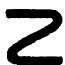
\includegraphics[keepaspectratio]{images/part001_a90573a3.jpg}}

命题 8. 设 \(f = \psi \circ g \circ \varphi\) 是连续映射 \(f: X \to Y\) 的典范分解，且设 \(R\) 表示等价关系

\[
f (x) = f (y).
\]

则下列三个条件等价：

\begin{enumerate}
\def\labelenumi{\alph{enumi})}
\item
  \(g\) 是由 \(\mathbf{X} / \mathbf{R}\) 到 \(f(\mathbf{X})\) 上的一个同胚。
\item
  在 \(f\) 之下，每个关于 \(\mathbf{R}\) 饱和的开集的像是子空间 \(f(\mathbf{X})\) 中的一个开集。
\item
  在 \(f\) 之下，每个关于 \(\mathbf{R}\) 饱和的闭集的像是子空间 \(f(\mathbf{X})\) 中的一个闭集。
\end{enumerate}

因为条件 b){[}resp. c){]}表达的是：X/R 中每个开（相应地，闭）集在 g 下的像是 \(f(\mathbf{X})\) 中的一个开（相应地，闭）集。

例。设 X 是拓扑空间，\((\mathbf{X}_{i})_{i\in I}\) 是 X 的一个覆盖，Y 是 X 的诸子空间 \(X_{v}\) 的和；则存在 Y 的一个分成既开又闭的子空间的分拆 \((\mathbf{Y}_{i})_{i\in I}\)，且对每个 \(i\in I\) 存在一个同胚 \(f_{i}:Y_{i}\to X_{i}\)。设 \(f:Y\to X\) 是与 \(f_{i}\)（在 \(Y_{i}\) 上，对每个 \(i\in I\)）相一致的连续映射，且设 R 是等价关系 \(f(x)=f(y)\)；于是商空间 Y/R 是把诸 \(Y_{i}\)"粘合"在一起得到的（§2，第 5 目）。考虑与 f 相伴的双射 \(g:Y/R\to X\)；一般说来 g 不是同胚，如下例所示：每个 \(X_{i}\) 都由单个点组成而 X 不是离散的。然而，若诸 \(X_{i}\) 的内部覆盖 X，或 \((\mathbf{X}_{i})\) 是 X 的一个局部有限闭覆盖，则 g 是同胚：因为若 U 是 Y 的任一关于 R 饱和的开子集，则对每个 \(i\in I\)，集合

\[
f (\mathbf {U}) \cap \mathbf {X} _ {i} = f _ {i} (\mathbf {U} \cap \mathbf {Y} _ {i})
\]

在 \(X_{i}\) 中是开集，且断言由第 1 目命题 3 得出。

下面的命题给出 \(g\) 是同胚的一个简单充分条件：

命题 9. 设 \(f: \mathbf{X} \to \mathbf{Y}\) 是一个连续满射，且设 \(\mathbf{R}\) 表示等价关系 \(f(x) = f(y)\)。若存在连续截面 \(s: \mathbf{Y} \to \mathbf{X}\)（与 \(f\) 相伴（《集合论》第二章，§ 3，第 8 目，定义 11）），则映射 \(g: \mathbf{X} / \mathbf{R} \to \mathbf{Y}\)（与 \(f\) 相伴）是一个同胚，且 \(s\) 是由 \(\mathbf{Y}\) 到子空间 \(s(\mathbf{Y})\)（\(\mathbf{X}\) 的子空间）上的一个同胚。

因为若 \(\varphi: \mathbf{X} \to \mathbf{X} / \mathbf{R}\) 是典范映射，则 \(g\) 与 \(\varphi \circ s\) 都是双射、连续且互逆；同样，\(s\) 与 \(f\) 在 \(s(\mathbf{Y})\) 上的限制都是双射、连续且互逆。

若 R 是拓扑空间 X 上的一个等价关系，且

\[
\varphi : \mathbf {X} \rightarrow \mathbf {X} / \mathbf {R}
\]

是典范映射，连续截面 \(s: \mathbf{X} / \mathbf{R} \to \mathbf{X}\)（与 \(\varphi\) 相伴）也称为 \(\mathbf{X}\) 关于 \(\mathbf{R}\) 的连续截面（参见《集合论》第二章，§ 6，第 2 目）；于是子空间 \(s(\mathbf{X} / \mathbf{R})\)（\(\mathbf{X}\) 的子空间）同胚于 \(\mathbf{X} / \mathbf{R}\)。若给定了 \(s(\mathbf{X} / \mathbf{R})\)，则 \(s\) 被唯一确定；\(s(\mathbf{X} / \mathbf{R})\) 常被（滥用语言地）称为 \(\mathbf{X}\) 关于 \(\mathbf{R}\) 的一个（连续）截面。

\pandocbounded{
\includegraphics[keepaspectratio]{images/part001_feb98675.jpg}}

拓扑空间关于一个等价关系的连续截面未必存在（习题 12）。

\subsection{子空间的商空间}

设 X 是拓扑空间，A 是 X 的一个子空间，R 是 X 上的一个等价关系，f 是典范映射 \(X \to X/R\)，g 是 f 在 A 上的限制。A 上的等价关系 \(g(x) = g(y)\) 恰是 R 在 A 上诱导的关系 \(R_{A}\)（《集合论》R，§ 5，第 5 目）。设 \(g = \psi \circ h \circ \varphi\) 是 g 的典范分解，于是若 j 是 A 到 X 中的典范单射，我们就有一个交换图 (*)

\begin{enumerate}
\def\labelenumi{(\Roman{enumi})}
\tightlist
\item
\end{enumerate}

\pandocbounded{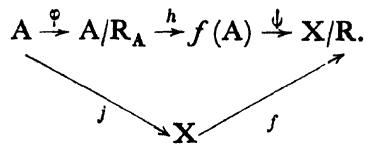
\includegraphics[keepaspectratio]{images/part001_6dc64900.jpg}}

命题 10. 典范双射 \(h: \mathbf{A} / \mathbf{R}_{\mathbf{A}} \to f(\mathbf{A})\) 是连续的。此外，下列三个命题等价：

\begin{enumerate}
\def\labelenumi{\alph{enumi})}
\item
  \(h\) 是一个同胚。
\item
  A 的每个关于 \(R_{A}\) 饱和的开子集都是 X 的某个关于 R 饱和的开子集与 A 的交。
\item
  A 的每个关于 \(R_{A}\) 饱和的闭子集都是 X 的某个关于 R 饱和的闭子集与 A 的交。
\end{enumerate}

命题的第一部分是直接的（第 5 目）。第二部分由第 5 目命题 8 得出：若 B 是 A 的关于 \(R_{A}\) 饱和的开（相应地，闭）子集，且 \(g(B) = f(B)\) 是 X/R 的某个开（相应地，闭）子集 C 与 \(f(A)\) 的交，则 B 是开（相应地，闭）子集 \(\overline{f}(C)\)

与 A 的交，该子集关于 R 饱和；反之，若 B 是某个关于 R 饱和的开（相应地，闭）子集 D 与 A 的交，则 \(f(\mathbf{B})\) 是 \(f(\mathbf{A})\) 与 \(f(\mathbf{D})\) 的交，而它在 X/R 中是开（相应地，闭）集。

推论 1. 若 A 是 X 的关于 R 饱和的开（相应地，闭）子集，则典范映射 \(h: \mathrm{A}/\mathrm{R}_{\mathrm{A}} \rightarrow f(\mathrm{A})\) 是一个同胚。

因为若 A 在 X 中开（相应地，闭）且关于 R 饱和，且 \(B \subset A\) 在 A 中开（相应地，闭）且关于 \(R_{A}\) 饱和，则 B 在 X 中开（相应地，闭）且关于 R 饱和。

推论 2. 若存在连续映射 \(u: \mathbf{X} \to \mathbf{A}\)，使得 \(u(x)\) 与 \(x \mod \mathbb{R}\) 同余（对每个 \(x \in \mathbf{X}\)），则 \(f(\mathbf{A}) = \mathbf{X} / \mathbb{R}\)，且典范映射 \(h: \mathbf{A} / \mathbb{R}_{\mathbf{A}} \to \mathbf{X} / \mathbb{R}\) 是一个同胚。

由于模 R 的每个等价类都与 A 相交，\(A/R_{A}\) 在 X/R 中的典范像是整个 X/R；另一方面，若 U 在 A 中开且关于 \(R_{A}\) 饱和，则由假设可知，\(\overline{u}^{1}(U)\) 是把 U 关于 R 饱和化所得到的集合；由于 u 连续，\(\overline{u}^{1}(U)\) 在 X 中是开集（§ 2，第 1 目，定理 1）。由这一事实并借助命题 10 即得推论。

例。* 设 R 表示实直线 R 上的等价关系 \(x \equiv y \pmod{1}\)（第 4 目，例），且设 A 表示闭区间 {[}0, 1{]}；A 包含模 R 每个等价类的至少一个点。\(\mathrm{A} / \mathbb{R}_{\mathbf{A}}\) 到环面 T 上的典范映射是一个同胚；因为若 F 在 A 中闭（从而在 R 中闭），则为把 F 关于关系 R 饱和化，须取诸闭集 \(\mathrm{F} + n\)（对所有 \(n \in \mathbf{Z}\)）的并，它们显然构成一个局部有限族，故其并是闭集（§ 1，第 5 目，命题 4）；断言由此得出。我们指出，\(\mathrm{A} / \mathbb{R}_{\mathbf{A}}\) 是把 A 中的点 0 与 1 等同起来得到的。*

\section{拓扑空间的积}

\subsection{积空间}

定义 1. 给定拓扑空间的一个族 \((\mathbf{X}_{t})_{t\in I}\)，这个族的积空间是指积集合 \(\mathbf{X} = \prod_{t\in I}\mathbf{X}_{t}\) 赋以诸 \(\mathbf{X}_{t}\) 的拓扑的积（§ 2，第 3 目，例 3）。诸空间 \(\mathbf{X}_{t}(t\in I)\) 称为 \(\mathbf{X}\) 的因子。

由 § 2 第 3 目命题 4，X 上的积拓扑以形如 \(\overline{\mathrm{pr}}_{t}^{1}(\mathbf{U}_{t})\) 的集合的有限交组成的集合 B 为一个基，其中 \(U_{t}\) 在 \(X_{t}\) 中是开集；这些集合是积 \(\prod_{i\in I}A_{i}\)，其中 \(A_{i}\) 在 \(X_{t}\) 中是开集（对每个 \(i\in I\)），且除去有限多个指标外 \(A_{i}=X_{t}\)。这些集合将称为初等集。

若 \(\mathfrak{B}_i\) 是 \(X_i\) 的拓扑的一个基（对每个 \(i \in I\)），则显然，初等集 \(\prod_{i \in I} A_i\)（满足 \(A_i \in \mathfrak{B}_i\)（对每个指标 \(i\)，只要 \(A_i \neq X_i\)））组成积拓扑的另一个基。于是，包含给定点 \(x \in X\) 的这种类型的初等集组成 \(x\) 的一个基本邻域系（\(\S 1\)，第 3 目，命题 3）。

若 I 是有限集，由诸因子 \(X_{i}\) 的拓扑构造积拓扑就更简单：初等集恰是积 \(\prod_{i\in I}A_{i}\)，其中 \(A_{i}\) 是 \(X_{i}\) 的任意开子集（对每个 \(i\in I\)）（参见习题 9）。

例。* 积 \(\mathbf{R}^n\)（\(n\) 个与实直线 \(\mathbf{R}\) 恒同的空间的积）称为 \(n\) 维实数空间；\(\mathbf{R}^2\) 也称为实平面（参见第六章，§ 1）。类似地，从有理直线 \(\mathbf{Q}\) 出发，我们定义 \(n\) 维有理数空间 \(\mathbf{Q}^n\)（当 \(n = 2\) 时称为有理平面）。

空间 \(\mathbf{R}^n\) 的拓扑以 \(n\) 个 \(\mathbf{R}\) 中开区间的所有积组成的集合为一个基，这些积称为 \(n\) 维开方块。包含点 \(x \in \mathbf{R}^n\) 的开方块组成这一点的一个基本邻域系。类似地，\(n\) 个 \(\mathbf{R}\) 中闭区间的积称为 \(n\) 维闭方块。以 \(x\) 为内点的闭方块也组成 \(x\) 的一个基本邻域系。对 \(\mathbf{Q}^n\) 有类似的结果。*

命题 1. 设 \(f = (f_{i})\) 是拓扑空间 \(Y\) 到积空间 \(X = \prod_{i \in I} X_{i}\) 中的一个映射。则 \(f\) 在点 \(a \in Y\) 处连续，当且仅当 \(f_{i}\)（对每个 \(i \in I\)）在 a 处连续。

由于 \(f_{t} = \mathrm{pr}_{t} \circ f\)，这只是 §2 第 3 目命题 4 的一个特例。

推论 1. 设 \((\mathbf{X}_t)_{i \in \mathbf{I}}\)、\((\mathbf{Y}_t)_{i \in \mathbf{I}}\) 是具有同一指标集的两个拓扑空间族。对每个 \(i \in \mathbf{I}\)，设 \(f_i\) 是 \(\mathbf{X}_t\) 到 \(\mathbf{Y}_t\) 中的一个映射。为使积映射 \(f: (x_i) \to (f_i(x_i))\)（它把

\[
\prod_ {i \in I} X _ {i} \quad i n t o \quad \prod_ {i \in I} Y _ {i}
\]

映到）在一点 \(a = (a_{i})\) 处连续，必须且只需 \(f_{i}\) 在 \(a_{i}\) 处连续（对每个 \(\mathfrak{t} \in \mathbf{I}\)）。

\(f\) 可以写成 \(x \to (f_{t}(\mathrm{pr}_{t}(x))\)，于是由命题 1，该条件是充分的。反之，对每个 \(x \in I\)，设 \(g_{x}\) 是 \(X_{x}\) 到 \(\prod_{i \in I} X_{i}\) 中的这样的映射：\(\mathrm{pr}_{x}(g_{x}(x_{x})) = x_{x}\)，且 \(\mathrm{pr}_{t}(g_{x}(x_{x})) = a_{t}\)（每当 \(i \neq x\)）；则由命题 1，\(g_{x}\) 在点 \(a_{x}\) 处连续。由于 \(f_{x} = \mathrm{pr}_{x} \circ f \circ g_{x}\)，由此得出：若 \(f\) 在 \(a\) 处连续，则 \(f_{x}\) 在 \(a_{x}\) 处连续。

推论 2. 设 X、Y 是两个拓扑空间。为使映射 \(f: \mathbf{X} \to \mathbf{Y}\) 连续，必须且只需映射 \(g: x \to (x, f(x))\) 是 X 到 \(f\) 的图象 G 上（把 G 看作积空间 \(\mathbf{X} \times \mathbf{Y}\) 的子空间）的一个同胚。

由于 \(f = \mathrm{pr}_2 \circ g\)，该条件是充分的。它也是必要的，因为若 \(f\) 连续，则 \(g\) 是双射且连续（命题 1），且 \(g\) 的逆是 \(\mathrm{pr}_1\) 在 \(G\) 上的限制，它是连续的（参见《集合论》第四章，§ 2，第 4 目，判别准则 CST 17）。

命题 2（拓扑积的结合性）. 设 \((\mathbf{X}_{\iota})_{\iota \in \mathbf{I}}\) 是拓扑空间的一个族，\((\mathbf{J}_{\kappa})_{\kappa \in \mathbf{K}}\) 是集合 I 的一个分拆，且对每个 \(\kappa \in \mathbf{K}\)，设 \(\mathbf{X}_{\kappa}^{\prime} = \prod_{i\in \mathbf{J}_{\kappa}}\mathbf{X}_{\iota}\) 是诸空间 \(\mathbf{X}_{\iota}\)（对 \(\iota \in \mathbf{J}_{\mathbf{K}}\)）的积。则积空间的典范映射
% semantic-fragments: legacy-input-seam
\relax{}
\[\prod_{i \in I} X_i\ \text{到积空间}\ \prod_{x \in K} X_x'\]

是一个同胚。

这是初始拓扑的传递性的一个特殊情形（§ 2，第 3 目，命题 5；参见《集合论》，第四章，§ 2，第 4 目，判别准则 CST 13）。

通常我们借助典范映射把积空间 \(\prod_{i\in I}X_i\) 与 \(\prod_{x\in X}X_x'\) 等同起来。

推论. 设 \(\sigma\) 是集合 I 的一个置换。则映射 \((x_{i})\to (x_{\sigma(i)})\) 是

\[
\prod_ {i \in I} X _ {i} \quad onto \quad \prod_ {i \in I} X _ {\sigma (i)}.
\]

在命题 2 中取 \(\mathbf{K} = \mathbf{I}\) 及 \(\mathbf{J}_t = \{\sigma(t)\}\)（对每个 \(t \in I\)）。

命题 3. 设 X 是一个集合，\((\mathbf{Y}_{t})_{t\in I}\) 是拓扑空间的一个族，且对每个 \(t\in I\)，设 \(f_{t}\) 是 X 到 \(Y_{t}\) 中的一个映射。设 f 是映射 \(x\to(f_{t}(x))\)，把 X 映入 \(Y=\prod_{t\in I}Y_{t}\)，并设 G 是 X 上使诸映射 \(f_{t}\) 连续的最粗的拓扑。则 G 是 Y 上的积拓扑在 \(f(\mathbf{X})\) 上诱导的拓扑在 f 下的逆像。

这是初始拓扑的传递性的又一个特殊情形（§ 2，第 3 目，命题 5；参见《集合论》，第四章，§ 2，第 4 目，判别准则 CST 15）。

推论. 对每个 \(t \in I\)，设 \(A_{t}\) 是 \(Y_{t}\) 的一个子空间。则在 \(A = \prod_{t \in I} A_{t}\) 上由 \(\prod_{t \in I} Y_{t}\) 上的积拓扑诱导的拓扑是诸子空间 \(A_{t}\) 的拓扑之积。

设 \(j_{i}\) 是典范单射 \(A_{i} \to Y_{i}\)，并对诸映射 \(f_{i} = j_{i} \circ \operatorname{pr}_{i}\) 应用命题 3（参见《集合论》，第四章，§ 2，第 4 目，判别准则 GST 14）。

\subsection{开集的截面；闭集的截面；开集的投影。部分连续性}

命题 4. 设 \(\mathbf{X}_1, \mathbf{X}_2\) 是两个拓扑空间；则对每个 \(a_1 \in \mathbf{X}_1\)，映射 \(x_2 \to (a_1, x_2)\) 是 \(\mathbf{X}_2\) 映到 \(\{a_1\} \times \mathbf{X}_2\)（\(\mathbf{X}_1 \times \mathbf{X}_2\) 的子空间）上的一个同胚。

这是把第 1 目命题 1 的推论 1 应用于常值函数 \(x_{2} \rightarrow a_{1}\) 而得的一个特殊情形。

映射 \(x_{2} \to (a_{1}, x_{2})\) 是关于等价关系 \(\mathrm{pr}_{2}z = \mathrm{pr}_{2}z'\)（在 \(\mathbf{X}_{1} \times \mathbf{X}_{2}\) 中）的一个连续截面（§ 3，第 5 目）；因此 \(\mathbf{X}_{1} \times \mathbf{X}_{2}\) 按此等价关系的商空间同胚于 \(\mathbf{X}_{2}\)。

推论. 截面 \(\mathbf{A}(x_1)\)（开（相应地，闭）集 \(\mathbf{A}\)——积 \(\mathbf{X}_1 \times \mathbf{X}_2\) 的——在任意一点 \(x_1 \in \mathbf{X}_1\)（*）处的截面）在 \(\mathbf{X}_2\) 中是开（相应地，闭）集。

命题 5. 积 \(X_{1} \times X_{2}\) 的开集 U 到任一因子上的投影是开集。

例如，我们有 \(\mathrm{pr}_2\mathrm{U} = \bigcup_{x_1\in X_1}\mathrm{U}(x_1)\)，于是由命题 4 的推论及公理 \((\mathbf{O}_{\mathbf{I}})\) 即得该命题。

\pandocbounded{
\includegraphics[keepaspectratio]{images/part001_fc188d82.jpg}}

注 1. \(\mathbf{X}_1 \times \mathbf{X}_2\) 的闭子集到一个因子上的投影未必是闭集。例如，在有理平面 \(\mathbf{Q}^2\) 中，方程为 \(x_1 x_2 = 1\) 的双曲线是闭集，但它的两个投影都等于 \(\mathbf{Q}\) 中点 0 的余集，而这不是闭集。

命题 6. 设 \(\mathbf{X}_1, \mathbf{X}_2, \mathbf{Y}\) 是三个拓扑空间，\(f\) 是积空间 \(\mathbf{X}_1 \times \mathbf{X}_2\) 到 \(\mathbf{Y}\) 中的一个映射。若 \(f\) 在点 \((a_1, a_2)\) 处连续，则部分映射 \(x_2 \to f(a_1, x_2)\)（\(\mathbf{X}_2\) 到 \(\mathbf{Y}\) 中的）在点 \(a_2\) 处连续。

因为这个映射是 \(f\) 与映射 \(x_{2} \to (a_{1}, x_{2})\) 的复合，故结论由命题 4 得出。

命题 6 常被表述为：两个变量的连续函数关于每个变量分别连续。

\pandocbounded{
\includegraphics[keepaspectratio]{images/part001_31ca3096.jpg}}

注 2. 由映射 \(f: \mathbf{X}_{1} \times \mathbf{X}_{2} \to \mathbf{Y}\) 所确定的所有部分映射都连续，而 \(f\) 在 \(\mathbf{X}_{1} \times \mathbf{X}_{2}\) 上不连续，这是可能的（参见第九章，§ 5，习题 23）。* 例如，若 \(f\) 是实平面 \(\mathbb{R}^{2}\) 到 \(\mathbb{R}\) 中的映射，其定义为

\[
f (x, y) = x y / \left(x ^ {2} + y ^ {2}\right) \quad \text { if } \quad (x, y) \neq (0, 0)
\]

且 \(f(0, 0) = 0\)，则所有部分映射都连续；但 \(f\) 在 \((0, 0)\) 处不连续，因为 \(f(x, x) = 1/2\)（对 \(x \neq 0\)）。

若 \(g\) 是 \(\mathbf{X}_1\) 到 \(\mathbf{Y}\) 中的一个映射，在点 \(a_1\) 处连续，则映射 \((x_1, x_2) \to g(x_1)\)（\(\mathbf{X}_1 \times \mathbf{X}_1 \to \mathbf{Y}\)）在所有点 \((a_1, x_2)\) 处连续，因为它是 \(g\) 与到 \(\mathbf{X}_1\) 上的投影的复合。

本小节的结果容易推广到拓扑空间的任意积 \(\prod_{i\in I}X_i\)，只需注意到对 I 的任意分拆 (J, K)，这个积同胚于积 \(\left(\prod_{i\in J}X_i\right)\times\left(\prod_{i\in K}X_i\right)\)（第 1 目，命题 2）。

\subsection{积中的闭包}

命题 7. 在积空间 \(\prod_{i\in I}X_i\) 中，集合的积 \(\prod_{i\in I}A_i\) 的闭包与它们的闭包的积 \(\prod_{i\in I}\overline{A}_i\) 相同。

设 \(a = (a_{t})\) 属于 \(\prod_{i} A_{i}\) 的闭包；则对每个 \(x \in I\)，\(a_{x} = \text{pr}_{x} a\) 属于 \(A_{x}\) 的闭包，这是由于 \(\text{pr}_{x}\) 的连续性（\(\S 2\)，第 1 目，定理 1），因此 \(a \in \prod_{i} \overline{A}_{i}\)。反之，设 \(b = (b_{i}) \in \prod_{i} \overline{A}_{i}\)，并设 \(\prod_{i} V_{i}\) 是包含 \(b\) 的任一初等集；对每个 \(i \in I\)，\(V_{i}\) 包含一点 \(x_{i} \in A_{i}\)；于是 \(\prod_{i} V_{i}\) 包含点 \((x_{i}) \in \prod_{i} A_{i}\)，因此 \(b\) 属于 \(\prod A_{i}\) 的闭包。

推论. 非空集合的积 \(\prod_{i} A_{i}\) 在积空间 \(\prod_{i} X_{i}\) 中是闭集，当且仅当 \(A_{i}\) 在 \(X_{i}\) 中是闭集（对每个 \(i \in I\)）。

若 I 是有限集，则积 \(\prod_{i\in I}A_i\) 是开集，只要 \(A_i\) 在 \(X_i\) 中是开集（对每个 \(i\in I\)）；但当 I 是无限集时情况不再如此。

命题 8. 设 \(a = (a_{i})\) 是积空间 \(X = \prod_{i \in I} X_{i}\) 的任一点；则集合 \(D\)——由这样的点 \(x \in X\) 组成：\(\operatorname{pr}_{i} x = a_{i}\) 对除有限多个外的指标 \(i\) 成立——在 \(X\) 中稠密。

对每个 \(x \in \mathbf{X}\) 及每个初等集 \(V = \prod_{i \in I} U_i\)（包含 \(x\) 的），我们有 \(U_i = X_i\)，但指标 \(i\) 属于有限子集 \(J\)（\(I\) 的）者除外；若取 \(y_i = x_i\)（对 \(i \in J\)）、\(y_i = a_i\)（对 \(i \notin J\)），则显然有

\[
y = (y _ {i}) \in D \quad \text { and } \quad y \in V;
\]

由此即得结论。

\subsection{拓扑空间的逆极限}

设 I 是一个偏序（但不一定有向）集（*），其上的序关系记作 \(\alpha \leqslant \beta\)。对每个 \(\alpha \in I\)，设 \(X_{\alpha}\) 是一个拓扑空间，且对每一对 \((\alpha, \beta)\)（满足 \(\alpha \leqslant \beta\)），设 \(f_{\alpha\beta}\) 是 \(X_{\beta}\) 到 \(X_{\alpha}\) 中的一个映射。我们说 \((X_{\alpha}, f_{\alpha\beta})\) 是拓扑空间的一个逆系统，如果：1) \((X_{\alpha}, f_{\alpha\beta})\) 是集合的一个逆系统；2) \(f_{\alpha\beta}\) 是连续映射（每当 \(\alpha \leqslant \beta\)）。设 X 表示集合 \(\varprojlim X_{\alpha}\)，且对每个 \(\alpha \in I\)，设 \(f_{\alpha}\) 是典范映射 \(X \to X_{\alpha}\)；则 X 上使诸 \(f_{\alpha}\) 连续的最粗的拓扑称为（关于 \(f_{\alpha\beta}\) 的）诸 \(X_{\alpha}\) 的拓扑的逆极限，而赋有该拓扑的集合 X 称为拓扑空间的逆系统 \((X_{\alpha}, f_{\alpha\beta})\) 的逆极限。每当我们把 \(\varprojlim X_{\alpha}\) 作为拓扑空间来谈论时，总应理解成这个空间的拓扑是诸 \(X_{\alpha}\) 的拓扑的逆极限，除非另有明确说明。

集合 X 是积 \(\prod_{\alpha\in I}X_{\alpha}\) 的由满足下列条件的点 x 组成的子集：

\[
\operatorname{pr} _ {\alpha} (x) = f _ {\alpha \beta} (\operatorname{pr} _ {\beta} (x))\tag{I}
\]

每当 \(\alpha \leqslant \beta\)。由第 1 目命题 3 可知，诸 \(X_{\alpha}\) 的拓扑的逆极限与 \(X\) 上由积空间 \(\prod_{\alpha \in I} X_{\alpha}\) 的拓扑诱导的拓扑相同。若对每个 \(\alpha \in I\)，\(Y_{\alpha}\) 是 \(X_{\alpha}\) 的子空间，且诸 \(Y_{\alpha}\) 构成诸 \(X_{\alpha}\) 的子集的一个逆系统（《集合论》，第三章，§ 7，第 2 目），则显然拓扑空间 \(\varprojlim Y_{\alpha}\) 是 \(\varprojlim X_{\alpha}\) 的一个子空间。

设 \((\mathbf{X}_{\alpha}^{\prime}, f_{\alpha\beta}^{\prime})\) 是以同一集合 I 为指标集的拓扑空间的另一个逆系统，且对每个 \(\alpha \in I\)，设 \(u_{\alpha}: X_{\alpha} \to X_{\alpha}^{\prime}\) 是连续映射，使得 \((u_{\alpha})\) 是映射的一个逆系统；则 \(u = \varprojlim u_{\alpha}\) 是 \(X = \varprojlim X_{\alpha}\) 到 \(X^{\prime} = \varprojlim X_{\alpha}^{\prime}\) 中的一个连续映射。因为若 \(f_{\alpha}^{\prime}\) 是典范映射 \(X^{\prime} \to X_{\alpha}^{\prime}\)，我们有 \(f_{\alpha}^{\prime} \circ u = u_{\alpha} \circ f_{\alpha}\)，从而 \(f_{\alpha}^{\prime} \circ u\) 对每个 \(\alpha \in I\) 连续，于是断言由 § 2 第 3 目命题 4 得出。

最后，设 I 是有向集，并设 J 是 I 的一个共尾子集；设 Z 是拓扑空间的逆系统 \((\mathbf{X}_{\alpha}, f_{\alpha\beta})_{\alpha\in\mathbf{J}, \beta\in\mathbf{J}}\) 的逆极限。则典范双射 \(g: X \to Z\)（《集合论》，第三章，§ 7，第 2 目，命题 3）是一个同胚。因为我们有 \(\operatorname{pr}_{\lambda}(g(x)) = \operatorname{pr}_{\lambda}(x)\)（对每个 \(\lambda \in J\)）；故 g 连续（第 1 目，命题 1）；又若 h 是 g 的逆，则对每个 \(\alpha \in I\)，存在 \(\lambda \in J\) 使 \(\alpha \leqslant \lambda\)，从而 \(\operatorname{pr}_{\alpha}(h(z)) = f_{\alpha\lambda}(\operatorname{pr}_{\lambda}(z))\)；由于诸 \(f_{\alpha\lambda}\) 连续，这表明 h 连续（第 1 目，命题 1）。

命题 9. 设 I 是有向集，J 是 I 的一个共尾子集。设 \((\mathbf{X}_{\alpha}, f_{\alpha \beta})\) 是以 I 为指标集的拓扑空间的一个逆系统；设 \(\mathbf{X} = \varprojlim \mathbf{X}_{\alpha}\)，并设 \(f_{\alpha}: \mathbf{X} \to \mathbf{X}_{\alpha}\) 是典范映射。则由诸集合 \(\overline{f}_{\alpha}^{1}(\mathbf{U}_{\alpha})\) 组成的族（其中 \(\alpha\) 取遍 J，\(\mathbf{U}_{\alpha}\) 取遍基 \(\mathfrak{B}_{\alpha}\)——\(\mathbf{X}_{\alpha}\) 的拓扑的基，对每个 \(\alpha \in \mathbf{J}\)）是 \(\mathbf{X}\) 的拓扑的一个基。

由 § 2 第 3 目可知，形如 \(\overline{f}_{\alpha}^{1}(\mathbf{U}_{\alpha})\)（\(\alpha \in \mathbf{I}\)，\(\mathbf{U}_{\alpha}\) 是 \(\mathbf{X}_{\alpha}\) 中的开集）的集合的有限交组成 \(\mathbf{X}\) 的拓扑的一个基。若 \((\alpha_i)_{1 \leqslant i \leqslant n}\) 是 \(\mathbf{I}\) 的一个有限指标族，则存在 \(\gamma \in \mathbf{J}\)，使 \(\alpha_i \leqslant \gamma\)（对 \(1 \leqslant i \leqslant n\)）；从而 \(f_{\alpha_i} = f_{\alpha_i \gamma} \circ f_\gamma\)；若令

\[
\begin{array}{c} \mathrm{V} _ {\gamma} = \bigcap_ {i} \overline {{f}} _ {\alpha_ {i} \gamma} ^ {1} (\mathrm{U} _ {\alpha_ {i}}), \\ \overline {{f}} _ {\gamma} ^ {1} (\mathrm{V} _ {\gamma}) = \bigcap_ {i} \overline {{f}} _ {\alpha_ {i}} ^ {1} (\mathrm{U} _ {\alpha_ {i}}); \end{array}
\]

则我们有

而 \(V_{\gamma}\) 是开集，因而是属于 \(\mathfrak{B}_{\gamma}\) 的一些集合之并。由此即得结论。

推论. 设 A 是 X 的一个子集，且用 \(A_{\alpha}\) 表示 \(f_{\alpha}(A)\)（对每个 \(\alpha \in I\)）。则：

\begin{enumerate}
\def\labelenumi{(\roman{enumi})}
\item
  诸 \(\mathbf{A}_{\alpha}\)（相应地，诸 \(\overline{\mathbf{A}}_{\alpha}\)）构成诸 \(\mathbf{X}_{\alpha}\) 的子集的一个逆系统，且 \(\overline{\mathbf{A}} = \bigcap_{\alpha} \overline{f}_{\alpha}^{1}(\overline{\mathbf{A}}_{\alpha}) = \varprojlim \overline{\mathbf{A}}_{\alpha}\)。
\item
  若 A 在 X 中是闭集，则 \(\mathbf{A} = \varprojlim \mathbf{A}_{\alpha} = \varprojlim \overline{\mathbf{A}}_{\alpha}\)。
\end{enumerate}

(i) 的第一个断言由诸关系 \(f_{\alpha} = f_{\alpha \beta} \circ f_{\beta}\)（对 \(\alpha \leqslant \beta\)）及诸 \(f_{\alpha \beta}\) 的连续性得出（§ 2，第 1 目，定理 1）。用 \(A'\) 表示

\[
\bigcap_ {\alpha} \overline {{f}} _ {\alpha} ^ {1} (\overline {{\mathrm{A}}} _ {\alpha});
\]

则显然 \(\mathbf{A}'\) 是闭集且包含 \(\mathbf{A}\)，从而 \(\overline{\mathbf{A}} \subset \mathbf{A}'\)。反之，设 \(x \in \mathbf{A}'\)；我们必须证明 \(x\) 属于 \(\mathbf{A}\) 的闭包。凭借命题 9，只须证明 \(x\) 的每个形如 \(\overline{f}_{\alpha}^{1}(\mathrm{U}_{\alpha})\) 的邻域（其中 \(\alpha \in \mathbf{I}\)，\(\mathbf{U}_{\alpha}\) 是 \(\mathbf{X}_{\alpha}\) 中的开集）都与 \(\mathbf{A}\) 相交。而按假设，\(f_{\alpha}(x) \in \mathbf{U}_{\alpha}\)，又因 \(f_{\alpha}(x) \in \overline{\mathbf{A}}_{\alpha}\)，我们有 \(\mathbf{U}_{\alpha} \cap \mathbf{A}_{\alpha} \neq \emptyset\)，这就意味着 \(\mathbf{A} \cap \overline{f}_{\alpha}^{1}(\mathbf{U}_{\alpha})\) 非空。

为建立 (ii)，只须注意，对 A 不加任何限制时，我们有 \(A \subset \varprojlim A_{\alpha} \subset \varprojlim \overline{A}_{\alpha}\)；而若 A 是闭集，则由 (i)

\[
\mathrm{A} = \varprojlim \overline {{\mathrm{A}}} _ {\alpha}
\]

便得 (ii)。

例. 设 I 是有向集，\((\mathbf{X}_{\alpha})_{\alpha \in I}\) 是集合 Y 的子集的一个族，使得 \(\mathbf{X}_{\alpha} \supset \mathbf{X}_{\beta}\)（每当 \(\alpha \leqslant \beta\)）。对每个 \(\alpha \in I\)，设 \(\mathfrak{G}_{\alpha}\) 是 \(\mathbf{X}_{\alpha}\) 上的一个拓扑，使得 \(\mathfrak{G}_{\beta}\) 都细于 \(\mathbf{X}_{\beta}\) 上由 \(\mathfrak{G}_{\alpha}\) 诱导的拓扑（每当 \(\alpha \leqslant \beta\)）。若取 \(f_{\alpha \beta}\) 为典范单射 \(\mathbf{X}_{\beta} \to \mathbf{X}_{\alpha}\)（对 \(\alpha \leqslant \beta\)），则 \(\varprojlim \mathbf{X}_{\alpha}\) 可以典范地等同于诸 \(\mathbf{X}_{\alpha}\) 的交 X，赋以诸拓扑之上确界（§ 2，第 3 目，例 2）——这些拓扑由诸 \(\mathfrak{G}_{\alpha}\) 在 X 上诱导。

\section{开映射与闭映射}

\subsection{开映射与闭映射}

定义 1. 设 X、X' 是两个拓扑空间。映射 f: X → X' 称为开（相应地，闭）映射，如果 X 的每个开（相应地，闭）集在 f 下的像在 X' 中是开（相应地，闭）集。

特别地，此时 \(f(\mathbf{X})\) 是 \(X'\) 的开（相应地，闭）子集。

例。1) 设 A 是拓扑空间 X 的一个子空间。则典范单射 \(j: \mathbf{A} \to \mathbf{X}\) 是开（相应地，闭）映射，当且仅当 A 在 X 中是开（相应地，闭）集（\(\S\) 3，第 1 目）。

\begin{enumerate}
\def\labelenumi{\arabic{enumi})}
\setcounter{enumi}{1}
\item
  为使双射 \(f\)（从拓扑空间 \(\mathbf{X}\) 到拓扑空间 \(\mathbf{X}'\) 上的）是一个同胚，必须且只需 \(f\) 连续且开，或连续且闭。
\item
  设 \(f\) 是集合 \(X\) 到拓扑空间 \(X'\) 上的一个满射；若给 \(X\) 赋以在 \(f\) 之下 \(X'\) 的拓扑的逆像这一拓扑（§ 2，第 3 目，例 1），则 \(f\) 连续、开且闭。
\item
  在积空间
\end{enumerate}

\[
\mathbf {X} = \prod_ {i \in \mathbf {I}} \mathbf {X} _ {i},
\]

中，每个投影 \(\mathbf{pr}_{t}:\mathbf{X}\to\mathbf{X}_{t}\) 都是连续的开映射，但未必是闭映射（§ 4，第 2 目，命题 5）。

* 5) 在 C 的开子集 A 上的全纯函数是 A 到 C 中的一个开映射。*

\begin{enumerate}
\def\labelenumi{\arabic{enumi})}
\setcounter{enumi}{5}
\tightlist
\item
  设 X、X' 是两个拓扑空间，f 是 X 到 X' 上的一个连续但非双连续的双射。则逆双射 g: \(X' \rightarrow X\) 是 \(X'\) 到 X 上的一个既开又闭的映射，但不连续。
\end{enumerate}

命题 1. 设 X、X'、X'' 是三个拓扑空间，并设 f: X → X'、g : X' → X'' 是两个映射。则：

\begin{enumerate}
\def\labelenumi{\alph{enumi})}
\item
  若 \(f\) 与 \(g\) 是开（相应地，闭）映射，则 \(g \circ f\) 亦然。
\item
  若 \(g \circ f\) 是开（相应地，闭）映射且 \(f\) 连续并满，则 \(g\) 是开（相应地，闭）映射。
\item
  若 \(g \circ f\) 是开（相应地，闭）映射且 \(g\) 连续并单，则 \(f\) 是开（相应地，闭）映射。
\end{enumerate}

a) 由定义 1 立即得出。为证 b)，只须注意，每个开（相应地，闭）子集 \(\mathbf{A}'\)（\(\mathbf{X}'\) 的）都可写成 \(f(\mathbf{A})\)，其中 \(\mathbf{A} = \overline{f}^{1}(\mathbf{A}')\) 在 \(\mathbf{X}\) 中是开（相应地，闭）集（\(\S 2\)，第 1 目，定理 1）；从而 \(g(\mathbf{A}') = g(f(\mathbf{A}))\) 在 \(\mathbf{X}''\) 中是开（相应地，闭）集。最后，为证 c)，我们注意，\(f(\mathbf{A}) = \overline{g}^{1}(g(f(\mathbf{A}))\) 对每个子集 \(\mathbf{A}\)（\(\mathbf{X}\) 的）成立；按假设，若 \(\mathbf{A}\) 在 \(\mathbf{X}\) 中是开（相应地，闭）集，则 \(g(f(\mathbf{A}))\) 在 \(\mathbf{X}''\) 中是开（相应地，闭）集，从而 \(f(\mathbf{A})\) 在 \(\mathbf{X}'\) 中是开（相应地，闭）集（\(\S 2\)，第 1 目，定理 1）。

命题 2. 设 X、Y 是两个拓扑空间，f 是 X 到 Y 中的一个映射。对 Y 的每个子集 T，用 \(f_{T}\) 表示 \(\overline{f}^{1}(T)\) 到 T 中的、在 \(\overline{f}^{1}(T)\) 上与 f 一致的映射。

\begin{enumerate}
\def\labelenumi{\alph{enumi})}
\item
  若 \(f\) 是开（相应地，闭）映射，则 \(f_{\mathbf{T}}\) 是开（相应地，闭）映射。
\item
  设 \((\mathbf{T}(\iota))_{\iota \in \mathbf{I}}\) 是 Y 的子集的一个族，其诸内部覆盖 Y，或者它是 Y 的一个局部有限闭覆盖；若所有 \(f_{\mathbf{T}(\iota)}\) 都是开（相应地，闭）映射，则 \(f\) 是开（相应地，闭）映射。
\item
  若 A 是 \(\overline{f}^{1}(\mathbf{T})\) 的开（相应地，闭）子集，则存在 X 的开（相应地，闭）子集 B，使 \(\mathbf{A} = \mathbf{B} \cap \overline{f}^{1}(\mathbf{T})\)，从而 \(f_{\mathbf{T}}(\mathbf{A}) = f(\mathbf{B}) \cap \mathbf{T}\)；按假设，\(f(\mathbf{B})\) 是开（相应地，闭）集，于是 \(f_{\mathbf{T}}(\mathbf{A})\) 在 \(\mathbf{T}\) 中是开（相应地，闭）集。
\item
  设 B 是 X 的开（相应地，闭）子集，并用 \(B_{i}\) 表示 \(\mathbf{B} \cap \overline{f}^{1}(\mathrm{T}(i))\)；则 \(f(\mathbf{B}) \cap \mathrm{T}(i) = f_{\mathbf{T}(i)}(\mathbf{B}_{i})\)。由于按假设 \(f_{\mathbf{T}(i)}(\mathbf{B}_{i})\) 在 \(\mathrm{T}(i)\) 中是开（相应地，闭）集，故由 § 3 第 1 目命题 3，\(f(\mathbf{B})\) 在 Y 中是开（相应地，闭）集。
\end{enumerate}

推论. 设 \((\mathbf{T}(\iota))_{\iota \in \mathbf{I}}\) 是 Y 的子集的一个族，其诸内部覆盖 Y，或者它是 Y 的一个局部有限闭覆盖。若 \(f: \mathbf{X} \to \mathbf{Y}\) 连续，且每个 \(f_{\mathbf{T}(\iota)}\) 都是 \(\overline{f}^1 (\mathbf{T}(\iota))\) 到 \(\mathbf{T}(\iota)\) 上的一个同胚，则 \(f\) 是 \(\mathbf{X}\) 到 \(\mathbf{Y}\) 上的一个同胚。

因为 \(f\) 显然是双射，且凭借命题 2 是开映射。

\subsection{开等价关系与闭等价关系}

定义 2. 拓扑空间 X 上的等价关系 R 称为开（相应地，闭）的，如果 X 到 X/R 上的典范映射是开（相应地，闭）映射。

这等价于说，X 的每个开（相应地，闭）子集关于 R 的饱和化在 X 中是开（相应地，闭）集（§ 3，第 4 目）。

例。1) 设 X 是拓扑空间，\(\Gamma\) 是 X 到自身的一些同胚所成的一个群，并设 R 是等价关系

\[
" \text { there   exists } \sigma \in \Gamma \text { such   that } y = \sigma (x)"
\]

（x 与 y 之间）（于是 R 是以 \(\Gamma\) 在 X 中的轨道为类的那个等价关系。关系 R 是开的，因为 X 的子集 A 关于 R 的饱和化是开集，诸 \(\sigma(\mathbf{A})\) 也是开集，从而它们的并也是开集。

* 在实直线 R 上，等价关系 \(x \equiv y \pmod{1}\) 是开的，因为它如上所述由平移群

\[
x \rightarrow x + n \quad (n \in \mathbf {Z})
\]

导出（见第三章，§ 2，第 4 目）。*

\begin{enumerate}
\def\labelenumi{\arabic{enumi})}
\setcounter{enumi}{1}
\tightlist
\item
  设 X 是子空间族 \((\mathbf{X}_{t})\) 的和，并设 X/R 是把诸 \(X_{t}\) 沿开子集 \(A_{tx}\) 借助双射 \(h_{xt}\) 粘合起来所得的空间（§ 2，第 5 目）；并设 \(h_{xt}\) 是 \(A_{tx}\) 到 \(A_{xt}\) 上的一个同胚（对每一对指标 \((t, x)\)）。
\end{enumerate}

则关系 R 是开的。因为若 U 在 X 中是开集，则 U 的饱和化是诸 \(h_{xt}(\mathbf{U} \cap \mathbf{A}_{\mathbf{tx}})\) 之并；由于 \(U \cap A_{tx}\) 在 \(A_{tx}\) 中是开集，故 \(h_{xt}(\mathbf{U} \cap \mathbf{A}_{\mathbf{tx}})\) 在 \(A_{xt}\) 中从而在 X 中是开集。

\begin{enumerate}
\def\labelenumi{\arabic{enumi})}
\setcounter{enumi}{2}
\tightlist
\item
  沿用例 2 的记号，现在设诸 \(\mathbf{A}_{\mathrm{tx}}\) 是闭集且诸 \(h_{xt}\) 是同胚；再设对每个指标 \(t\)，只有有限多个指标 \(x\) 使 \(\mathbf{A}_{\mathrm{tx}} \neq \emptyset\)（亦即每个 \(\mathbf{X}_t\) 只与有限多个 \(\mathbf{X}_x\) 相“粘”）。则关系 R 是闭的。因为若 F 是 X 的任一闭子集，则 F 的饱和化是诸集合 \(h_{xt}(\mathbf{F} \cap \mathbf{A}_{\mathrm{tx}}) \subset \mathbf{A}_{xt}\) 之并；所作的假定蕴含这一族是局部有限的，且 \(h_{xt}(\mathbf{F} \cap \mathbf{A}_{\mathrm{tx}})\) 在 \(\mathbf{A}_{xt}\) 中从而在 X 中是闭集。于是结论由 § 2 第 5 目命题 4 得出。
\end{enumerate}

命题 3. 设 X、Y 是两个拓扑空间，设 \(f: \mathbf{X} \to \mathbf{Y}\) 是连续映射，设 R 是 X 上的等价关系 \(f(x) = f(y)\)，并设 \(\mathbf{X} \xrightarrow{p} \mathbf{X}/\mathbf{R} \xrightarrow{h} f(\mathbf{X}) \xrightarrow{i} \mathbf{Y}\) 是 \(f\) 的典范分解。则下列三个命题等价：

\begin{enumerate}
\def\labelenumi{\alph{enumi})}
\item
  \(f\) 是开映射。
\item
  三个映射 \(p, h, i\) 都是开映射。
\item
  等价关系 R 是开的，h 是同胚，且 \(f(\mathbf{X})\) 是 Y 的开子集。
\end{enumerate}

还有，若把前面命题中的“开”处处换为“闭”，该命题仍成立。

由于单射 \(i\) 连续，由第 1 目命题 1c) 可知，若 \(f\) 是开映射，则 \(h \circ p\) 亦然；由于 \(p\) 满且连续，命题 1b) 表明 \(h\) 是开映射；\(h\) 无论如何是连续双射；于是 \(h\) 是同胚，从而由第 1 目命题 1a)，\(p = \overline{h}^1 \circ (h \circ p)\) 是开映射。又有{[}第 1 目，命题 1b){]}，\(i \circ h\) 是开映射；故{[}第 1 目，命题 1a){]}，\(i = (i \circ h) \circ \overline{h}^1\) 亦然。这就证明了 a) 蕴含 b)。反之，第 1 目命题 1a) 表明 b) 蕴含 a)。最后，b) 与 c) 的等价性由定义立即得出。

闭映射情形的证明，作适当改动后是类似的。

命题 4. 设 R 是拓扑空间 X 上的开（相应地，闭）等价关系，f 是典范映射 X → X/R。设 A 是 X 的一个子集，且下列两个条件之一成立：a) A 在 X 中是开（相应地，闭）集。

\begin{enumerate}
\def\labelenumi{\alph{enumi})}
\setcounter{enumi}{1}
\tightlist
\item
  A 关于 R 是饱和的。
\end{enumerate}

则在 A 上诱导的关系 \(R_{A}\) 是开（相应地，闭）的，且 \(A/R_{A}\) 到 \(f(A)\) 上的典范映射是同胚。

考虑 § 3 第 6 目的交换图 (1)，它给出 \(f \circ j\) 的典范分解。在条件 a) 下，\(j\) 是开（相应地，闭）映射，而按假设 \(f\) 亦然；故 \(f \circ j\) 是开（相应地，闭）映射{[}第 1 目，命题 1 a){]}，结论由命题 3 得出。在条件 b) 下，我们有

\[
\mathbf {A} = \overline {{{f}}} ^ {1} (f (\mathbf {A})),
\]

且 \(h \circ \varphi\) 是 A 到 \(f(A)\) 中的、在 A 上与 \(f\) 一致的映射；凭借第 1 目命题 2 a)，\(h \circ \varphi\) 是开（相应地，闭）映射，而把命题 3 应用于 \(h \circ \varphi\)，又得出结论。

\subsection{开映射特有的性质}

命题 5. 设 X、Y 是两个拓扑空间，f 是 X 到 Y 中的一个映射，B 是 X 的拓扑的一个基。则下列命题等价：

\begin{enumerate}
\def\labelenumi{\alph{enumi})}
\item
  \(f\) 是开映射。
\item
  对每个 \(\mathbf{U} \in \mathfrak{B}\)，\(f(\mathbf{U})\) 在 \(\mathbf{Y}\) 中是开集。
\item
  对每个 \(x \in \mathbf{X}\) 及每个邻域 \(\mathbf{V}\)（\(x\) 的，\(\mathbf{X}\) 中的），\(f(\mathbf{V})\) 都是 \(f(x)\) 在 \(\mathbf{Y}\) 中的一个邻域。
\end{enumerate}

a) 与 b) 的等价性由定义及 \((\mathrm{O}_{\mathrm{I}})\) 立即得出；a) 与 c) 的等价性是 § 1 第 2 目命题 1 的推论。

命题 6. 设 R 是拓扑空间 X 上的一个等价关系；则下列三个条件等价：

\begin{enumerate}
\def\labelenumi{\alph{enumi})}
\item
  关系 \(\mathbf{R}\) 是开的。
\item
  每个关于 R 饱和的子集，其内部关于 R 是饱和的。
\item
  每个关于 R 饱和的子集，其闭包关于 R 是饱和的。
\end{enumerate}

取余集（§ 1，第 6 目，公式 (2)）可见 b) 与 c) 等价。我们来证 b) 蕴含 a)：设条件 b) 成立，并设 U 是 X 的开子集，V 是它关于 R 的饱和化；则 \(\dot{V} \supset U\)，又因按假设 \(\dot{V}\) 是饱和的，故 \(\dot{V} = V\)，从而 U 的饱和化是开集。反之，设条件 a) 成立，并设 A 是一个饱和集；若 B 是 \(\mathring{A}\) 的饱和化，则 \(\mathring{A} \subset B \subset A\)，又因按假设 B 是开集，故 \(B = \mathring{A}\)。

命题 7. 设 R 是拓扑空间 X 上的开等价关系，并设 \(\varphi: \mathbf{X} \to \mathbf{X}/\mathbf{R}\) 是典范映射。若 A 是 X 的任一关于 R 饱和的子集，则 \(\varphi(\mathbf{A})\) 在 X/R 中的闭包（相应地，内部）是 \(\varphi(\overline{\mathbf{A}})\)（相应地，\(\varphi(\mathring{\mathbf{A}})\)）。

该命题的两个断言中的每一个都可由另一个通过取余集并利用 § 1 第 6 目公式 (2) 及下述事实导出：若 B 是 X 的饱和子集，则 \(\varphi(\complement B) = \complement \varphi(B)\)。凭借命题 6，\(\overline{A}\) 是饱和的；从而 \(\varphi(\overline{A})\) 在 \(X/R\) 中是闭集，又因 \(A \subset \overline{A}\)，我们有 \(\overline{\varphi(A)} \subset \varphi(\overline{A})\)，从而 \(\varphi(A) \subset \varphi(\overline{A})\)。但由 \(\varphi\) 连续，\(\varphi(\overline{A}) \subset \overline{\varphi(A)}\)（\(\S 2\)，第 1 目，定理 1），由此即得结论。

命题 8. 设 \((\mathbf{X}_t)_{t \in \mathbf{I}}\)、\((\mathbf{Y}_t)_{t \in \mathbf{I}}\) 是以同一集合 I 为指标集的两个拓扑空间族。对每个 \(t \in \mathbf{I}\)，设 \(f_t\) 是 \(\mathbf{X}_t\) 到 \(\mathbf{Y}_t\) 中的一个开映射，并设除去有限多个指标外 \(f_t\) 都是满射。则积映射 \(f: (x_t) \to (f_t(x_t))\)（\(\prod_{t \in \mathbf{I}} \mathbf{X}_t\) 到 \(\prod_{t \in \mathbf{I}} \mathbf{Y}_t\) 中的）是开映射。

凭借命题 5，我们只须证明 \(f\) 的任意初等集 \(\prod_{t \in I} A_t\)（\(\prod_{t \in I} X_t\) 中的）的像在 \(\prod_{t \in I} Y_t\) 中是开集。而这个像是 \(\prod_{t \in I} f_t(A_t)\)，且诸假设蕴含：\(f_t(A_t)\) 在 \(Y_t\) 中是开集（对每个 \(t \in I\)），且除去有限多个指标外 \(f_t(A_t) = Y_t\)；由此即得结论。

推论. 设 \((\mathbf{X}_t)_{t \in I}\) 是拓扑空间的一个族，且对每个 \(t \in I\)，设 \(\mathbf{R}_t\) 是 \(\mathbf{X}_t\) 上的一个等价关系，并设 \(f_t\) 是典范映射 \(\mathbf{X}_t \to \mathbf{X}_t / \mathbf{R}_t\)。设 \(\mathbf{R}\) 是 \(\mathbf{X} = \prod_{t \in I} \mathbf{X}_t\) 中的等价关系“对每个 \(t \in I\)，\(\operatorname{pr}_t(x) = \operatorname{pr}_t(y) (\bmod \mathbf{R}_t)"\)

（\(x\) 与 \(y\) 之间），并设 \(f\) 是积映射 \((x_{t}) \to (f_{t}(x_{t}))\)（\(X\) 到 \(\prod_{t \in I} (X_{t}/R_{t})\) 中的）。若诸关系 \(R_{t}\) 都是开的，则关系 \(R\) 是开的，且与 \(f\) 相伴的双射是 \(X/R\) 到 \(\prod_{t \in I} (X_{t}/R_{t})\) 上的一个同胚。

R 是关系 \(f(x)=f(y)\)。由于由上面的命题 8 及 § 4 第 1 目命题 1 的推论 1，f 连续且开，故结论由第 2 目命题 3 得出。

特别地，若 R（相应地，S）是拓扑空间 X（相应地，Y）上的开等价关系，则

\[
(\mathbf {X} \times \mathbf {Y}) / (\mathbf {R} \times \mathbf {S}) \quad \text { onto } \quad (\mathbf {X} / \mathbf {R}) \times (\mathbf {Y} / \mathbf {S})
\]

\pandocbounded{
\includegraphics[keepaspectratio]{images/part001_bebaa45c.jpg}}

的典范双射是一个同胚。若不假定 R 与 S 都是开的，则这个双射连续但未必是同胚，即使关系 R、S 之一是相等关系（习题 6）亦然。

\subsection{闭映射特有的性质}

命题 9. 设 X、X' 是两个拓扑空间。映射 \(f: \mathbf{X} \to \mathbf{X}'\) 连续且闭的充分必要条件是：对 X 的每个子集 A，\(f(\overline{\mathbf{A}}) = \overline{f(\mathbf{A})}\)。

该条件是充分的，因为它显然蕴含 \(f\) 是闭映射，且由 § 2 第 1 目定理 1，它也蕴含 \(f\) 连续。反之，若 \(f\) 连续且闭，则由 § 2 第 1 目定理 1，我们有 \(f(\mathbf{A}) \subset f(\overline{\mathbf{A}}) \subset \overline{f(\mathbf{A})}\)；又按假设 \(f(\overline{\mathbf{A}})\) 在 \(\mathbf{X}'\) 中是闭集；从而 \(f(\overline{\mathbf{A}}) = \overline{f(\mathbf{A})}\)。

命题 10. 设 R 是拓扑空间 X 上的一个等价关系。则 R 是闭的，当且仅当模 R 的每个等价类 M 都具有由关于 R 饱和的邻域组成的一个基本邻域系。

设 R 是闭的，并设 U 是 M 的任一开邻域；由于 \(F = \complement U\) 在 X 中是闭集，F 关于 R 的饱和化 S 在 X 中是闭集。由于 M 关于 R 是饱和的，我们有 \(M \cap S = \varnothing\)，从而 \(V = \complement S\) 是 M 的一个开邻域，它关于 R 饱和且含于 U。

为证其逆，设 F 是 X 的任一闭子集。设 T 是 F 关于 R 的饱和化，设 x 是 \(\complement T\) 的一点，并设 M 是 x 的等价类；则 \(M \cap T = \varnothing\)，从而更有 \(M \cap F = \varnothing\)，于是 U = \(\complement F\) 是 M 的一个邻域。因此存在 M 的一个邻域 \(V \subset U\)，使 V 关于 R 饱和；V 不与 F 相交，故不与 T 相交，从而 \(\complement T\) 是 M 的、因而是 x 的一个邻域。这表明 \(\complement T\) 是开集（§ 1，第 2 目，命题 1），亦即 T 是闭集。

注. 命题 10 蕴含以下事实：若 R 是闭的，且用 \(\varphi\) 表示典范映射 \(X \to X/R\)，则对每个 \(x \in X\) 以及 \(x\) 的等价类在 X 中的每个邻域 U，\(\varphi(U)\) 都是 \(\varphi(x)\) 在 X/R 中的一个邻域。应当仔细注意，这一断言决不蕴含：对 \(x\) 的每个邻域 V，\(\varphi(V)\) 都是 \(\varphi(x)\) 的邻域；换言之（第 3 目，命题 5），闭等价关系未必是开的（习题 2）。反过来，开等价关系也未必是闭的（第 1 目，例 4）；

\pandocbounded{
\includegraphics[keepaspectratio]{images/part001_bfecd507.jpg}}

因为若 U 是某个等价类 M 在 X 中的一个邻域，则对每个 \(x \in M\) 以及 x 的每个邻域 \(V \subset U\)，V 的饱和化固然是 M 在 X 中的一个邻域，但这个邻域未必含于 U。

最后，存在除相等关系之外既开又闭的等价关系（习题 3），也存在既不开又不闭的等价关系（\(§\ 8\)，习题 10）。

\section{滤子}

\subsection{滤子的定义}

定义 1. 集合 X 上的滤子是 X 的子集所成的一个集合 F，它具有下列性质：

（F \(_{I}\)）X 的每个包含 F 中某个集合的子集都属于 F。

\((\mathbf{F}_{\mathrm{II}})\) \(\mathfrak{F}\) 的集合的每个有限交都属于 \(\mathfrak{F}\)。

\((\mathbf{F}_{\mathrm{III}})\) 空集不属于 \(\mathfrak{F}\)。

由 \((\mathbf{F}_{\mathbf{II}})\) 与 \((\mathbf{F}_{\mathbf{III}})\) 可知，F 的集合的每个有限交都非空。

X 上的滤子 \(\mathfrak{F}\) 在 X 上定义了一个结构，其公理为 \((\mathrm{F_I})\)、\((\mathrm{F_{II}})\) 与 \((\mathrm{F_{III}})\)；这个结构称为滤集结构，而赋以该结构的集合 X 称为被 \(\mathfrak{F}\) 滤化的集合。

公理 \((\mathbf{F}_{\mathrm{II}})\) 等价于下列两条公理的合取：\((\mathbf{F}_{\mathrm{II}a})\) F 中两个集合的交属于 F。

\((\mathbf{F}_{\mathrm{II}b})\) X 属于 \(\mathfrak{F}\)。

公理 \((\mathbf{F}_{\mathbf{II}\ \mathbf{b}})\) 与 \((\mathbf{F}_{\mathbf{III}})\) 表明空集上不存在滤子。

为使满足 \((\mathbf{F}_{\mathbf{I}})\) 的子集族也满足 \((\mathbf{F}_{\mathbf{II}\mathbf{b}})\)，必须且只需它非空。满足 \((\mathbf{F}_{\mathbf{I}})\) 的子集族也满足 \((\mathbf{F}_{\mathbf{III}})\)，当且仅当它异于 \(\mathfrak{P}(\mathbf{X})\)。

滤子的例子. 1) 若 \(\mathbf{X} \neq \emptyset\)，则仅由 \(\mathbf{X}\) 组成的子集族是 \(\mathbf{X}\) 上的一个滤子。更一般地，\(\mathbf{X}\) 中包含给定非空子集 \(\mathbf{A}\)（\(\mathbf{X}\) 的）的所有子集所成之集是 \(\mathbf{X}\) 上的一个滤子。

\begin{enumerate}
\def\labelenumi{\arabic{enumi})}
\setcounter{enumi}{1}
\item
  在拓扑空间 X 中，X 的任一非空子集 A 的所有邻域所成之集（特别地，X 中一点的所有邻域所成之集）是一个滤子，称为 A 的邻域滤子。
\item
  若 X 是无限集，则 X 的有限子集的余集组成一个滤子的元素。由 \(\geqslant0\) 的整数组成的集 N 的有限子集的余集所成的滤子称为 Fréchet 滤子。
\end{enumerate}

\subsection{滤子的比较}

定义 2. 给定同一集合 X 上的两个滤子 \(\mathfrak{F}\)、\(\mathfrak{F}'\)，称 \(\mathfrak{F}'\) 细于 \(\mathfrak{F}\)，或称 \(\mathfrak{F}\) 粗于 \(\mathfrak{F}'\)，如果 \(\mathfrak{F} \subset \mathfrak{F}'\)。若还有 \(\mathfrak{F} \neq \mathfrak{F}'\)，则称 \(\mathfrak{F}'\) 严格细于 \(\mathfrak{F}\)，或称 \(\mathfrak{F}\) 严格粗于 \(\mathfrak{F}'\)。

若两个滤子中一个细于另一个，则称这两个滤子可比较。X 上所有滤子所成之集按关系“F 粗于 F”排序；这个关系是由 \(\mathfrak{P}(\mathfrak{P}(\mathbf{X}))\) 中的包含关系诱导的。

设 \((\mathfrak{F}_t)_{\iota \in I}\) 是集合 \(X\) 上滤子的任一非空族（因而 X 必非空）；则集合

\[
\mathfrak {F} = \bigcap_ {i \in I} \mathfrak {F} _ {i}
\]

满足公理 \((\mathbf{F}_{\mathbf{I}})\)、\((\mathbf{F}_{\mathbf{II}})\) 与 \((\mathbf{F}_{\mathbf{III}})\)，从而是一个滤子；F 称为滤子族 \((\mathfrak{F}_{i})_{i\in\mathbf{I}}\) 的交，并且显然是 X 上所有滤子之有序集中诸 \(F_{i}\) 所成之集的下确界。

由单独一个集合 X 组成的滤子是 X 上所有滤子之有序集的最小元。我们将在第 4 目看到，若 X 的元素多于一个，则 X 上所有滤子所成之集没有最大元。

给定集合 X 的一个子集族 \(\mathfrak{G}\)，我们来考察 X 上是否存在包含 \(\mathfrak{G}\) 的滤子。若这样的滤子存在，则由 \((\mathrm{F}_{\mathrm{II}})\)，它也包含集 \(\mathfrak{G}'\)（\(\mathfrak{G}\) 中集合的有限交所成之集，包括 X，即 \(\mathfrak{G}\) 的空子集之交）；因此这样的滤子存在的一个必要条件是 X 的空子集不属于 \(\mathfrak{G}'\)。这个条件也是充分的，因为由 \((\mathrm{F}_{\mathrm{I}})\)，任何包含 \(\mathfrak{G}'\) 的滤子也包含集 \(\mathfrak{G}''\)（X 中包含 \(\mathfrak{G}'\) 中某个集合的子集所成之集）。而 \(\mathfrak{G}''\) 显然满足 \((\mathrm{F}_{\mathrm{I}})\)；它满足 \((\mathrm{F}_{\mathrm{II}})\)（由 \(\mathfrak{G}'\) 的定义）；最后，它满足 \((\mathrm{F}_{\mathrm{III}})\)，因为 X 的空子集不属于 \(\mathfrak{G}'\)。于是 \(\mathfrak{G}''\) 是包含 \(\mathfrak{G}\) 的最粗滤子，而且我们已证明：

命题 1. X 上存在包含 X 的子集所成之集 \(\mathfrak{G}\) 的滤子的充分必要条件是：\(\mathfrak{G}\) 的任何有限子集的交都非空。

上面定义的滤子 \(\mathfrak{G}''\) 称为由 \(\mathfrak{G}\) 生成的滤子，而 \(\mathfrak{G}\) 称为 \(\mathfrak{G}''\) 的一个子基。

例. 设 \(\mathfrak{S}\) 是集合 X 的子集所成的任一集，并设 \(\mathfrak{C}\) 是由 \(\mathfrak{S}\) 生成的 X 上的拓扑（\(\S\) 2，第 3 目，例 II）。由于 \(\mathfrak{S}\) 中集合的有限交所成之集是 \(\mathfrak{C}\) 的一个基，故由上面命题 1 的证明以及 \(\S\) 1 第 3 目命题 3 可知，对每个 \(x \in X\)，\(x\) 关于 \(\mathcal{C}\) 的邻域滤子由集合 \(\mathfrak{S}(x)\)（\(\mathfrak{S}\) 中包含 \(x\) 的集合所成之集）生成。

推论 1. 设 \(\mathfrak{F}\) 是集合 X 上的一个滤子，A 是 X 的一个子集。则存在滤子 \(\mathfrak{F}'\)，它细于 \(\mathfrak{F}\) 且使得 \(A \in \mathfrak{F}'\)，当且仅当 A 与 \(\mathfrak{F}\) 的所有集合相交。

推论 2. 滤子所成之集 \(\Phi\)（非空集合 \(\mathbf{X}\) 上的）在 \(\mathbf{X}\) 上所有滤子所成之集中有上确界，当且仅当对所有有限序列 \((\mathfrak{F}_i)_{1\leqslant i\leqslant n}\)（\(\Phi\) 的元素的）以及所有 \(\mathrm{A}_i\in \mathfrak{F}_i\)（\(1\leqslant i\leqslant n\)），交 \(\mathrm{A}_1\cap \dots \cap \mathrm{A}_n\) 都非空。

因为这一条件表明并 \(\mathfrak{G}\)——诸滤子 \(\mathfrak{F} \in \Phi\) 之并——满足命题 1 的条件。

推论 3. 非空集合 X 上所有滤子所成之有序集是归纳的。

因为滤子的每个线性有序集 \(\Phi\)（\(X\) 上的）都满足命题 1 的推论 2 的条件，这是由于按假设诸集合 \(A_{i}\) 都属于同一个 \(\mathfrak{F}_{j}\)，于是可以应用 \((\mathbf{F}_{\mathrm{II}})\)。

\subsection{滤子的基}

若 \(\mathfrak{G}\) 是 X 上滤子 \(\mathfrak{F}\) 的一个子基（第 2 目），则 \(\mathfrak{F}\) 一般并不是 X 中包含 \(\mathfrak{G}\) 中某个集合的子集所成之集；为使 \(\mathfrak{G}\) 具有这一性质，必须且只需 \(\mathfrak{G}\) 中集合的每个有限交都包含 \(\mathfrak{G}\) 的某个集合。于是有下列命题：

命题 2. 设 \(\mathfrak{B}\) 是集合 X 的子集所成之集。则 X 中包含 \(\mathfrak{B}\) 中某个集合的子集所成之集是一个滤子，当且仅当 \(\mathfrak{B}\) 具有下列两条性质：

（B \(_{I}\)）B 中两个集合的交包含 B 的某个集合。

（B \(_{II}\)）B 非空，且 X 的空子集不属于 B。

定义 3. 集合 X 的满足公理（B \(_{I}\)）与（B \(_{II}\)）的子集所成之集 B 称为它所生成的滤子的基。若两个滤子基生成同一个滤子，则称它们等价。

若 \(\mathfrak{G}\) 是滤子 \(\mathfrak{F}\) 的一个子基，则集合 \(\mathfrak{G}'\)（\(\mathfrak{G}\) 中集合的有限交所成之集）是 \(\mathfrak{F}\) 的一个基（第 2 目）。

命题 3. 子集 \(\mathfrak{B}\)——滤子 \(\mathfrak{F}\)（\(\mathbf{X}\) 上的）的子集——是 \(\mathfrak{F}\) 的基，当且仅当 \(\mathfrak{F}\) 的每个集合都包含 \(\mathfrak{B}\) 的某个集合。

若 \(\mathfrak{B}\) 是 \(\mathfrak{F}\) 的基，则显然 \(\mathfrak{F}\) 的每个集合都包含 \(\mathfrak{B}\) 的某个集合；反之，若 \(\mathfrak{F}\) 的每个集合都包含 \(\mathfrak{B}\) 的某个集合，则 \(X\) 中包含 \(\mathfrak{B}\) 的某个集合的子集所成之集与 \(\mathfrak{F}\) 一致（由 \((\mathbf{F}_{\mathbf{I}})\)）。

例如，Fréchet 滤子（第 1 目）是被视为按关系 \(\leqslant\) 定向的有序集 N 的截面滤子。设 \(\mathfrak{F}\) 是集合 Z 上的一个滤子。由于 \(\mathfrak{F}\) 按关系 \(\supset\) 是有向的{[}由公理 \((\mathrm{F}_{\mathrm{II}})\){]}，我们可以在 \(\mathfrak{F}\) 上定义截面滤子；这里 \(\mathfrak{F}\) 相对于集合 A\(\in\mathfrak{F}\) 的截面是所有 M\(\in\mathfrak{F}\)（满足 M\(\subset\)A 者）所成之集 S(A)。这个滤子称为滤子 \(\mathfrak{F}\) 的截面滤子。

命题 4. 在集合 X 上，滤子 \(\mathfrak{F}'\)（以 \(\mathfrak{B}'\) 为基的）细于滤子 \(\mathfrak{F}\)（以 \(\mathfrak{B}\) 为基的），当且仅当 \(\mathfrak{B}\) 的每个集合都包含 \(\mathfrak{B}'\) 的某个集合。

这是定义 2 和定义 3 的直接推论。

推论. 集合 X 上两个滤子基 B、B' 等价，当且仅当 B 的每个集合都包含 B' 的某个集合，且 B' 的每个集合都包含 B 的某个集合。

滤子基的例子. 1) 设 X 是拓扑空间。命题 3 表明，一点 \(x \in X\) 的邻域滤子的基恰好就是 \(x\) 的基本邻域系（§ 1，第 3 目，定义 5）。

\begin{enumerate}
\def\labelenumi{\arabic{enumi})}
\setcounter{enumi}{1}
\tightlist
\item
  设 X 是关于关系 \((\sigma)\) 的非空有向集（《集合论》，第三章，§ 1，第 10 目）。对每个 \(a \in X\)，集合 \(S(a)\)——由所有这样的 \(x \in X\)（满足 \(a(\sigma)x\) 者）组成——称为 X 相对于元素 a 的截面。于是 X 的截面所成之集 S 是一个滤子基，因为它显然满足 \((\mathbf{B}_{\mathbf{II}})\)，且若 a、b 是 X 的任意两个元素，则按假设存在元素 \(c \in X\) 使得 \(a(\sigma)c\) 与 \(b(\sigma)c\)，从而
\end{enumerate}

\[
\mathbf {S} (c) \subset \mathbf {S} (a) \cap \mathbf {S} (b),
\]

于是 \((\mathbf{B}_{\mathbf{I}})\) 得到满足。由 S 生成的滤子称为有向集 X 的截面滤子。

\subsection{超滤子}

定义 4. 集合 X 上的超滤子是这样的滤子 F：X 上不存在严格细于 F 的滤子（换言之，即 X 上所有滤子之有序集中的极大元素）。

由于 X 上所有滤子之有序集是归纳的（第 2 目，命题 1，推论 3），Zorn 引理（《集合论》，R，§ 6，第 10 目）表明：

定理 1. 若 F 是集合 X 上的任一滤子，则存在细于 F 的超滤子。

命题 5. 设 \(\mathfrak{F}\) 是集合 \(\mathbf{X}\) 上的超滤子。若 \(\mathbf{A}\) 与 \(\mathbf{B}\) 是 \(\mathbf{X}\) 的两个子集，且 \(\mathbf{A} \cup \mathbf{B} \in \mathfrak{F}\)，则或者 \(\mathbf{A} \in \mathfrak{F}\)，或者 \(\mathbf{B} \in \mathfrak{F}\)。

若命题不真，则存在 X 的子集 A 与 B，使得 A∉F、B∉F 且 A∪B∈F。设 G 是 X 中满足 A∪M∈F 的子集 M 所成之集。直接验证可知 G 是 X 上的滤子，且 G 严格细于 F，因为 B∈G；但这与 F 是超滤子的假设矛盾。

推论. 若子集的一个有限序列 \((\mathbf{A}_i)_{1 \leqslant i \leqslant n}\)（\(\mathbf{X}\) 的）之并属于超滤子 \(\mathfrak{F}\)，则至少有一个 \(\mathbf{A}_i\) 属于 \(\mathfrak{F}\)。

对 n 用归纳法证明。

特别地，若 \((\mathbf{A}_i)_{1\leqslant i\leqslant n}\) 是 \(\mathbf{X}\) 的一个覆盖，则至少有一个 \(\mathbf{A}_i\) 属于 \(\mathfrak{F}\)。

命题 5 刻画了超滤子；更一般地，我们有：

命题 6. 设 \(\mathfrak{G}\) 是集合 X 上某个滤子的子基。若对 X 的每个子集 Y，或者 \(Y \in \mathfrak{G}\)，或者 \(\complement Y \in \mathfrak{G}\)，则 \(\mathfrak{G}\) 是 X 上的超滤子。

设 \(\mathfrak{F}\) 是包含 \(\mathfrak{G}\) 的滤子（按假设它是存在的）；则 \(\mathfrak{F}\) 与 \(\mathfrak{G}\) 一致；因为若 \(Y \in \mathfrak{F}\)，则 \(\complement Y \notin \mathfrak{F}\)；于是 \(\complement Y \notin \mathfrak{G}\)，从而 \(Y \in \mathfrak{G}\)。

超滤子的例子. 非空集合 X 中包含给定元素 \(a \in X\) 的所有子集所成之集是一个超滤子；因为它是滤子，且若 Y 是 X 的任一子集，则或者 \(a \in Y\)，或者 \(a \in \complement Y\)。这样的超滤子称为平凡超滤子。

除这个例子之外，我们将只在用到定理 1（从而用到选择公理）时才证明超滤子（即使在可数无限集上的超滤子）的存在性。

注. 若 X 至少含两个元素，则 X 上至少有两个不同的超滤子，因而 X 上滤子的有序集没有最大元。

命题 7. 每个滤子 \(\mathfrak{F}\)（集合 \(X\) 上的）都是细于 \(\mathfrak{F}\) 的诸超滤子之交。

显然这个交包含 \(\mathfrak{F}\)。反之，设 \(A\) 是 \(X\) 的不属于 \(\mathfrak{F}\) 的子集，并用 \(A'\) 表示 \(\complement A\)；\(A\) 不包含 \(\mathfrak{F}\) 的任何集合；于是每个 \(M \in \mathfrak{F}\) 都与 \(A'\) 相交，从而（第 2 目，命题 1，推论 1）存在滤子 \(\mathfrak{F}'\)，它细于 \(\mathfrak{F}\) 且包含 \(A'\)。若 \(\mathfrak{U}\) 是细于 \(\mathfrak{F}'\) 的超滤子（定理 1），则由此可知 \(A \notin \mathfrak{U}\)。证明完毕。

\subsection{诱导滤子}

命题 8. 设 \(\mathfrak{F}\) 是集合 X 上的滤子，A 是 X 的子集。则迹 \(\mathfrak{F}_{\mathrm{A}}\)（\(\mathfrak{F}\) 在 A 上的）是滤子，当且仅当 \(\mathfrak{F}\) 的每个集合都与 A 相交。

由 \((\mathbf{M} \cap \mathbf{N}) \cap \mathbf{A} = (\mathbf{M} \cap \mathbf{A}) \cap (\mathbf{N} \cap \mathbf{A})\) 可见 \(\mathfrak{F}_{\mathbf{A}}\) 满足 \((\mathbf{F}_{\mathbf{II}})\)；再者，若 \(\mathbf{M} \cap \mathbf{A} \subset \mathbf{P} \subset \mathbf{A}\)，则 \(\mathbf{P} = (\mathbf{M} \cup \mathbf{P}) \cap \mathbf{A}\)，从而 \(\mathfrak{F}_{\mathbf{A}}\) 满足 \((\mathbf{F}_{\mathbf{I}})\)。于是 \(\mathfrak{F}_{\mathbf{A}}\) 是滤子，当且仅当它满足 \((\mathbf{F}_{\mathbf{III}})\)，亦即当且仅当 \(\mathfrak{F}\) 的每个集合都与 \(\mathbf{A}\) 相交。

特别地，若 \(\mathbf{A} \in \mathfrak{F}\)，则 \(\mathfrak{F}_{\mathbf{A}}\) 是 \(\mathbf{A}\) 上的滤子（由 \((\mathbf{F}_{\mathbf{II}})\) 与 \((\mathbf{F}_{\mathbf{III}})\)）。

定义 5. 设 A 是集合 X 的子集，F 是 X 上的滤子。若 F 在 A 上的迹是 A 上的滤子，则称此滤子为 F 在 A 上诱导的滤子。

若滤子 \(\mathfrak{F}\)（\(X\) 上的）在 \(A \subset X\) 上诱导出一个滤子，则在 \(A\) 上，\(\mathfrak{F}\) 的一个基的迹是 \(\mathfrak{F}_A\) 的基，由第 3 目命题 3。

例. 设 X 是拓扑空间，A 是 X 的子集，x 是 X 的一点。为使 x 的邻域滤子 B 在 A 上的迹是 A 上的滤子，必须且只需 x 的每个邻域都与 A 相交，亦即 x 属于 A 的闭包（§ 1，第 6 目，定义 10）。

这个诱导滤子的例子之所以重要，有两个原因：第一，它在极限理论中起重要作用（§ 7，第 5 目）；第二，每个滤子都可以用这种方式定义。事实上，设 F 是集合 X 上的滤子，并设 X' 是在 X 上添加一个新元素 ω 所得的集合，其中 X 与 \{ω\} 在 X' 中的余集视为同一（《集合论》，R，§ 4，第 5 目）；设 F' 是 X' 上由形如 M ∪ \{ω\} 的集合组成的滤子，其中 M 取遍 F。对 X' 的每个点 x ≠ ω，设 B(x) 是 X' 中包含 x 的所有子集所成之集，并设 B(ω) 为 F'；于是 x ∈ X' 的诸 B(x) 显然满足公理 (V₁)、(V₂)、(V₃) 与 (V₄)，从而在 X' 上定义了一个拓扑，使它们成为各点的邻域滤子。最后，在此拓扑下 ω 属于 X 的闭包，且 F 是由 F' = B(ω) 在 X 上诱导的。这样在 X' 上定义的拓扑（相应地，赋以该拓扑的集合 X'）称为伴随于 F 的拓扑（相应地，拓扑空间）。

命题 9. 超滤子 \(\mathfrak{U}\)（集合 \(X\) 上的）在子集 \(A\)（\(X\) 的）上诱导出滤子，当且仅当 \(A \in \mathfrak{U}\)；且当此条件满足时，\(\mathfrak{U}_A\) 是 \(A\) 上的超滤子。

这是第 4 目命题 5 与命题 6 的直接推论。

\subsection{滤子基的像与逆像}

设 \(\mathfrak{B}\) 是集合 \(\mathbf{X}\) 上的滤子基，并设 \(f\) 是 \(\mathbf{X}\) 到集合 \(\mathbf{X}'\) 中的映射；则 \(f(\mathfrak{B})\) 是 \(\mathbf{X}'\) 上的滤子基，因为由关系 \(\mathbf{M} \neq \emptyset\) 可得 \(f(\mathbf{M}) \neq \emptyset\)，且我们有 \(f(\mathbf{M} \cap \mathbf{N}) \subset f(\mathbf{M}) \cap f(\mathbf{N})\)。若 \(\mathfrak{B}_1\) 是细于以 \(\mathfrak{B}\) 为基之滤子的某个滤子的基，则 \(f(\mathfrak{B}_1)\) 是细于以 \(f(\mathfrak{B})\) 为基之滤子的某个滤子的基（第 3 目，命题 4）。

命题 10. 若 \(\mathfrak{B}\) 是集合 X 上的超滤子基，且 \(f\) 是 X 到集合 \(\mathbf{X}'\) 中的映射，则 \(f(\mathfrak{B})\) 是 \(\mathbf{X}'\) 上的超滤子基。

设 \(\mathbf{M}'\) 是 \(\mathbf{X}'\) 的子集。若 \(\overline{f}^{1}(\mathbf{M}')\) 包含某个集合 \(\mathbf{M}\)（属于 \(\mathfrak{B}\)），则 \(\mathbf{M}'\) 包含 \(f(\mathbf{M})\)；若不然，则 \(\complement \overline{f}^{1}(\mathbf{M}') = \overline{f}^{1}(\complement \mathbf{M}')\) 包含某个集合 \(\mathbf{N}\)（\(\mathfrak{B}\) 中的）（第 4 目，命题 5），从而 \(\complement \mathbf{M}'\) 包含 \(f(\mathbf{N})\)。于是结论由第 4 目命题 6 得出。

特别考虑 \(f\) 是典范单射 \(\mathbf{A} \to \mathbf{X}\)（\(\mathbf{A}\) 为集合 \(\mathbf{X}\) 的子集）的情形。若 \(\mathfrak{B}\) 是 \(\mathbf{A}\) 上的滤子基，则 \(f(\mathfrak{B})\) 是 \(\mathbf{X}\) 上的滤子基。滤子 \(\mathfrak{F}\)（\(\mathbf{X}\) 上的，由 \(f(\mathfrak{B})\) 生成的）称为由 \(\mathfrak{B}\)（把 \(\mathfrak{B}\) 视为 \(\mathbf{X}\) 上的滤子基时）生成的滤子。若 \(\mathfrak{B}\) 是 \(\mathbf{A}\) 上的超滤子基，则由命题 10，它也是 \(\mathbf{X}\) 上的超滤子基。

接下来考察滤子基的逆像是否为滤子基。设 \(\mathfrak{B}'\) 是集合 \(\mathbf{X}'\) 上的滤子基，并设 \(f\) 是集合 \(\mathbf{X}\) 到 \(\mathbf{X}'\) 中的映射；则 \(\overline{f}^{1}(\mathfrak{B}')\) 是 \(\mathbf{X}\) 上的滤子基，当且仅当 \(\overline{f}^{1}(\mathbf{M}') \neq \emptyset\)（对每个 \(\mathbf{M}' \in \mathfrak{B}'\)）。这是关系 \(\overline{f}^{1}(\mathbf{M}' \cap \mathbf{N}') = \overline{f}^{1}(\mathbf{M}') \cap \overline{f}^{1}(\mathbf{N}')\) 与第 3 目定义 3 的直接推论。这个条件也可以表述为：\(\mathfrak{B}'\) 的每个集合都与 \(f(\mathbf{X})\) 相交{[}或者说 \(\mathfrak{B}'\) 在 \(f(\mathbf{X})\) 上的迹是一个滤子基{]}。若此条件满足，则 \(f(\overline{f}^{1}(\mathfrak{B}'))\) 是以 \(\mathfrak{B}\) 为基的滤子的一个较细滤子的基。

若 \(\mathfrak{B}\) 是 \(\mathbf{X}\) 上的滤子基，则显然 \(\mathfrak{B}' = f(\mathfrak{B})\) 满足上述条件；于是 \(\overline{f}^1 (f(\mathfrak{B}))\) 是粗于以 \(\mathfrak{B}\) 为基之滤子的某个滤子的基。

设 A 是集合 X 的子集，\(\varphi\) 是典范单射 \(A \rightarrow X\)；若 B 是 X 上的滤子基，则 \(\overline{\varphi}^{1}(\mathfrak{B})\) 与 \(B_{A}\) 相同。若利用上述条件把它表示为 A 上的滤子基，我们就重新得到第 5 目命题 8 的一部分。

\subsection{滤子的积}

设 \((\mathbf{X}_t)_{t \in I}\) 是集合的族，且对每个 \(t \in I\)，设 \(\mathfrak{B}_t\) 是 \(\mathbf{X}_t\) 上的滤子基。设 \(\mathfrak{B}\) 是积集 \(\mathbf{X} = \prod_{t \in I} \mathbf{X}_t\) 中形如 \(\prod_{t \in I} \mathbf{M}_t\) 的子集所成之集，其中除有限个指标外 \(\mathbf{M}_t = \mathbf{X}_t\)，且 \(\mathbf{M}_t \in \mathfrak{B}_t\)（对每个 \(t\)，它使 \(\mathbf{M}_t \neq \mathbf{X}_t\)）。公式 \(\left(\prod_{t \in I} \mathbf{M}_t\right) \cap \left(\prod_{t \in I} \mathbf{N}_t\right) = \prod_{t \in I} (\mathbf{M}_t \cap \mathbf{N}_t)\) 表明 \(\mathfrak{B}\) 是 \(\mathbf{X}\) 上的滤子基。注意，以 \(\mathfrak{B}\) 为基的滤子也由诸集合 \(\overline{\mathrm{pr}}_x^1 (\mathbf{M}_x)\) 生成，其中 \(\mathbf{M}_x\in \mathfrak{B}_x\) 且 \(\pmb{x}\) 取遍 I，因为

\[
\overline {{\mathrm{pr}}} _ {x} ^ {1} \left(\mathbf {M} _ {x}\right) = \mathbf {M} _ {x} \times \prod_ {i \neq x} \mathbf {X} _ {i}.
\]

定义 6. 给定滤子 \(\mathfrak{F}_t\)（每个集合 \(X_t\) 上的，集合族 \((X_t)_{t \in I}\) 的成员），诸滤子 \(\mathfrak{F}_t\) 的积是 \(X = \prod_{t \in I} X_t\) 上以 \(X\) 的形如 \(\prod_{t \in I} M_t\) 的子集所成之集为基的滤子，其中 \(M_t \in \mathfrak{F}_t\)（对每个 \(t \in I\)），且除有限个指标外 \(M_t = X_t\)。积滤子记作 \(\prod_{t \in I} \mathfrak{F}_t\)。

读者容易验证，诸滤子 \(\mathfrak{F}_i\) 的积也可以定义为最粗滤子 \(\mathfrak{G}\)（\(\mathbf{X}\) 上的，使 \(\mathrm{pr}_i(\mathfrak{G}) = \mathfrak{F}_i\) 对每个 \(i \in I\) 成立）。

前面的评注表明，若 \(\mathfrak{B}_{t}\) 是 \(\mathfrak{F}_{t}\) 的基（对每个 \(t\in I\)），则 \(\mathfrak{B}\) 是积滤子 \(\prod \mathfrak{F}_{t}\) 的基（第 3 目，命题 3）。

在拓扑空间的积 \(X = \prod_{i \in I} X_i\) 上，任一点 \(x = (x_i)\) 的邻域滤子是诸 \(x_i\) 的邻域滤子之积（§ 4，第 1 目）。

积滤子 \(\mathfrak{F} = \prod_{i\in I}\mathfrak{F}_i\) 的构造在指标集 \(I\) 有限时更简单：此时 \(\mathfrak{F}\) 的基由所有的积 \(\prod_{i\in I}M_i\) 组成，其中 \(M_i\in \mathfrak{F}_i\)（对每个 \(i\in I\)）。若 \(I = \{1,2,\ldots,n\}\)，我们记

\[
\mathfrak {F} _ {1} \times \mathfrak {F} _ {2} \times \dots \times \mathfrak {F} _ {n}
\]

以代替 \(\prod_{i\in I}\mathfrak{F}_i\)

\subsection{初等滤子}

定义 7. 设 \((x_{n})_{n\in \mathbb{N}}\) 是集合 \(\mathbf{X}\) 的元素的无穷序列。与序列 \((x_{n})\) 相伴的初等滤子是由 Fréchet 滤子（第 1 目）经映射 \(n\to x_n\)（\(\mathbf{N}\) 到 \(\mathbf{X}\) 中的）所得的像生成的滤子。等价地说，与 \((x_{n})\) 相伴的初等滤子是子集 \(\mathbf{M}\)（\(\mathbf{X}\) 的，使得都有 \(x_{n}\in \mathbf{M}\)——除去 \(n\) 的有限多个值外）所成之集。若用 \(\mathbf{S}_n\) 表示所有这样的 \(x_{p}\)（满足 \(p\geqslant n\)）所成之集，则诸集合 \(\mathbf{S}_n\) 组成与序列 \((x_{n})\) 相伴的初等滤子的一个基。

与序列 \((x_{n})\) 的无穷子列相伴的初等滤子细于与 \((x_{n})\) 相伴的初等滤子（参看习题 15）。

按定义，每个初等滤子都有可数基。反之：命题 11. 若滤子 F 有可数基，则它是细于 F 的诸初等滤子之交。

把 \(\mathfrak{F}\) 的可数基排成序列 \((\mathbf{A}_n)_{n\in \mathbb{N}}\)；若令

\[
\mathrm{B} _ {n} = \bigcap_ {p = 0} ^ {n} \mathrm{A} _ {p},
\]

则诸 \(B_{n}\) 仍组成 F 的基（第 3 目，命题 3），且对每个 n 有 \(B_{n+1} \subset B_{n}\)。设 \(a_{n}\) 是 \(B_{n}\) 的任一元素（对每个 \(n \in N\)）；则显然 F 粗于与 \((a_{n})\) 相伴的初等滤子。于是细于 F 的诸初等滤子之交 S 存在且细于 F；若 S 严格细于 F，则存在集合 \(M \in S\)，使对每个 n 有 \(B_{n} \cap CM \neq \varnothing\)；若 \(b_{n} \in B_{n} \cap CM\)，则与序列 \((b_{n})\) 相伴的初等滤子细于 F 且不含 M。这与 S 的定义矛盾。

注. 粗于某个具有可数基的滤子的滤子未必具有可数基；例如，若 X 是不可数无限集，则由 X 的有限子集的余集组成的滤子没有可数基（否则 X 的有限子集所成之集将是可数的，与假设相反）；然而这个滤子粗于由 X 的互异元素组成的无穷序列所相伴的每个初等滤子。

\subsection{关于滤子的芽}

设 \(\mathfrak{F}\) 是集合 \(X\) 上的滤子。在集合 \(\mathfrak{P}(X)\)（\(X\) 的所有子集所成之集）上，关系

\[
" \text { there   exists } \quad V \in \mathfrak {F} \text { such   that } \quad M \cap V = N \cap V"
\]

（在 M 与 N 之间）是一个等价关系 R，因为 R 显然是自反且对称的，且若 M、N、P 是 X 的三个子集，满足 \(M \cap V = N \cap V\) 与 \(N \cap W = P \cap W\)，其中 V 与 W 属于 F，则由此可得 \(M \cap (V \cap W) = N \cap (V \cap W) = P \cap (V \cap W)\) 且 \(V \cap W \in F\)，故 R 是传递的。X 的子集 M 模 R 的等价类称为 M 关于 F 的芽；商集 \(\mathfrak{P}(X)/R\) 称为 X 的子集（关于 F）的芽所成之集。

映射 \((\mathbf{M},\mathbf{N})\to \mathbf{M}\cap \mathbf{N}\) 与 \((\mathbf{M},\mathbf{N})\rightarrow \mathbf{M}\cup \mathbf{N}\)（定义在

\[
\mathfrak {P} (\mathbf {X}) \times \mathfrak {P} (\mathbf {X})
\]

上）到 \(\mathfrak{P}(\mathbf{X})\) 中，它们与等价关系 \(\mathbf{R} \times \mathbf{R}\) 和 \(\mathbf{R}\) 相容（《集合论》，R，§ 5，第 8 目）。因为若 \(\mathbf{M} \equiv \mathbf{M}'\) (mod R) 且 \(\mathbf{N} \equiv \mathbf{N}'\) (mod R)，则存在 \(\mathbf{V}\) 与 \(\mathbf{W}\)（\(\mathfrak{F}\) 中的），使得

\[
\begin{array}{r l} & {\mathbf {M} \cap \mathbf {V} = \mathbf {M} ^ {\prime} \cap \mathbf {V} \qquad \mathrm{and} \qquad \mathbf {N} \cap \mathbf {W} = \mathbf {N} ^ {\prime} \cap \mathbf {W},} \\ {\mathrm{so\ that}} & {(\mathbf {M} \cap \mathbf {N}) \cap (\mathbf {V} \cap \mathbf {W}) = (\mathbf {M} ^ {\prime} \cap \mathbf {N} ^ {\prime}) \cap (\mathbf {V} \cap \mathbf {W})} \\ {\mathrm{and}} & {(\mathbf {M} \cup \mathbf {N}) \cap (\mathbf {V} \cap \mathbf {W}) = (\mathbf {M} \cap (\mathbf {V} \cap \mathbf {W})) \cup (\mathbf {N} \cap (\mathbf {V} \cap \mathbf {W}))} \\ & {\qquad = (\mathbf {M} ^ {\prime} \cap (\mathbf {V} \cap \mathbf {W})) \cup (\mathbf {N} ^ {\prime} \cap (\mathbf {V} \cap \mathbf {W}))} \\ & {\qquad = (\mathbf {M} ^ {\prime} \cup \mathbf {N} ^ {\prime}) \cap (\mathbf {V} \cap \mathbf {W}).} \end{array}
\]

过渡到商，这些映射诱导出 \((\mathfrak{P}(\mathbf{X}) / \mathbf{R}) \times (\mathfrak{P}(\mathbf{X}) / \mathbf{R})\) 到 \(\mathfrak{P}(\mathbf{X}) / \mathbf{R}\) 中的两个映射，我们（滥用术语）分别记作 \((\xi, \eta) \to \xi \cap \eta\) 与 \((\xi, \eta) \to \xi \cup \eta\)。直接验证即可确认：关于这些合成法则{[}在整个 \(\mathfrak{P}(\mathbf{X}) / \mathbf{R}\) 上定义的{]}，每个元素都是幂等的，且每个法则都是交换的、结合的，并对另一个法则可分配。此外，关系 \(\xi = \xi \cap \eta\) 与 \(\eta = \xi \cup \eta\) 等价；若（滥用术语）把它们记作 \(\xi \subset \eta\)，则容易验证这个关系是 \(\mathfrak{P}(\mathbf{X}) / \mathbf{R}\) 上的一个序，关于此序 \(\mathfrak{P}(\mathbf{X}) / \mathbf{R}\) 是一个格，它以 \(\varnothing\) 的芽为最小元，以 \(\mathbf{X}\) 的芽为最大元。注意，关系 \(\xi \subset \eta\) 表示存在 \(\mathbf{M} \in \xi\)、\(\mathbf{N} \in \eta\) 与 \(\mathbf{V} \in \mathfrak{F}\)，使得 \(\mathbf{M} \cap \mathbf{V} \subset \mathbf{N} \cap \mathbf{V}\)。

现在设 \(X'\) 是另一个集合，并设 \(\Phi\) 是 F 的某个集合到 \(X'\) 中的所有映射所成之集。\(\Phi\) 上的关系

“存在 \(V \in F\)，使得 f 与 g 在 \(V\) 上都有定义且相等”

（在 \(f\) 与 \(g\) 之间）是一个等价关系 \(\mathbf{S}\)；显然 \(\mathbf{S}\) 是自反且对称的，且若 \(f, g, h\) 是 \(\Phi\) 的三个元素，使得 \(f\) 与 \(g\) 在 \(\mathbf{V} \in \mathfrak{F}\) 上有定义，而 \(g\) 与 \(h\) 在 \(\mathbf{W} \in \mathfrak{F}\) 上有定义且相等，则 \(f\) 与 \(h\) 在 \(\mathbf{V} \cap \mathbf{W} \in \mathfrak{F}\) 上有定义且相等，故 \(\mathbf{S}\) 是传递的。模 \(\mathbf{S}\) 的等价类——这里指映射 \(f\)（集合 \(\mathbf{V} \in \mathfrak{F}\) 到 \(\mathbf{X}'\) 中的）的等价类——称为 \(f\)（关于 \(\mathfrak{F}\)）的芽，而商集 \(\tilde{\Phi} = \Phi / \mathbf{S}\) 称为 \(\mathbf{X}\) 到 \(\mathbf{X}'\) 中的映射（关于 \(\mathfrak{F}\)）的芽所成之集。

注. 1) 每个映射 \(f\)——把子集 \(M\)（\(X\) 的）映入 \(X'\)，其中 \(M\) 属于 \(\mathfrak{F}\)——都模 \(S\) 等价于某个映射 \(f_1\)（\(X\) 到 \(X'\) 中的）（这证明上述术语是合理的）：只需把 \(f\) 延拓到 \(X\) 上，例如在 \(X - M\) 上给它取常值即可。

\begin{enumerate}
\def\labelenumi{\arabic{enumi})}
\setcounter{enumi}{1}
\tightlist
\item
  特征函数 \(\varphi_{\mathbf{M}}\) 与 \(\varphi_{\mathbf{N}}\)——子集 \(\mathbf{M}\) 与 \(\mathbf{N}\)（\(\mathbf{X}\) 的）的特征函数——关于 \(\mathfrak{F}\) 有相同的芽，当且仅当 \(\mathbf{M}\) 与 \(\mathbf{N}\) 关于 \(\mathfrak{F}\) 有相同的芽。
\end{enumerate}

设 \(X''\) 是第三个集合，\(\varphi\) 是 \(X'\) 到 \(X''\) 中的映射，\(\Phi'\) 是 \(\mathfrak{F}\) 的某个集合到 \(X''\) 中的所有映射所成之集。对每个 \(f \in \Phi\)，\(\varphi \circ f\) 属于 \(\Phi'\)；此外，立即可见若 \(g \in \Phi\) 与 \(f\) 关于 \(\mathfrak{F}\) 有相同的芽，则 \(\varphi \circ f\) 与 \(\varphi \circ g\) 关于 \(\mathfrak{F}\) 有相同的芽。

因此这个芽只依赖于芽 \(\tilde{f}\)（\(f\) 关于 \(\mathfrak{F}\) 的），记作 \(\varphi(\tilde{f})\)。这样我们就定义了一个映射（滥用术语，记作 \(\varphi\)），从集合 \(\tilde{\Phi}\)（X 到 \(\mathrm{X}'\) 中的映射的芽所成之集）到集合 \(\tilde{\Phi}'\)（X 到 \(\mathrm{X}''\) 中的映射的芽所成之集）。

现在设 \(\mathbf{X}_i^{\prime}\)（\(1 \leqslant i \leqslant n\)）是一些集合，而

\[
\mathbf {Y} = \prod_ {i = 1} ^ {n} \mathbf {X} _ {i} ^ {\prime}
\]

是它们的积；用 \(\Phi_i\)（相应地，\(\Phi\)）表示 \(\mathfrak{F}\) 的某个集合到 \(\mathbf{X}_i'\)（相应地，\(\mathbf{Y}\)）中的所有映射所成之集。若 \(f_i \in \Phi_i\)（对 \(1 \leqslant i \leqslant n\)），且 \(\mathbf{M}_i \in \mathfrak{F}\) 是 \(f_i\) 的定义域，则映射 \(t \to (f_1(t), \ldots, f_n(t))\) 定义在

\[
\bigcap_ {i = 1} ^ {n} \mathbf {M} _ {i}
\]

上，从而属于 \(\Phi\)；我们（滥用术语）把这个映射记作 \((f_1, \ldots, f_n)\)。此外，若 \(f_i\) 与 \(g_i\) 都属于 \(\Phi_i\) 且关于 \(\mathfrak{F}\) 有相同的芽（对 \(1 \leqslant i \leqslant n\)），则立即可见 \((f_1, \ldots, f_n)\) 与 \((g_1, \ldots, g_n)\) 关于 \(\mathfrak{F}\) 有相同的芽；因此这个芽只依赖于诸芽 \(\tilde{f}_i\)（\(f_i\) 的）。若把它记作 \(\Gamma(\tilde{f}_1, \ldots, \tilde{f}_n)\)，则 \(\Gamma\) 显然是积集

\[
\prod_ {i = 1} ^ {n} \tilde {\Phi} _ {i}
\]

到集合 \(\tilde{\Phi}\) 上的一个双射，其中 \(\tilde{\Phi}_i\)（相应地，\(\tilde{\Phi}\)）表示 X 到 \(\mathbf{X}_i'\)（相应地，Y）中的映射关于 \(\mathfrak{F}\) 的芽所成之集；因此，只要没有混淆的危险，我们将（滥用术语）一般用 \((\tilde{f}_1, \ldots, \tilde{f}_n)\) 代替 \(\Gamma(\tilde{f}_1, \ldots, \tilde{f}_n)\)。

由以上所述，每个映射 \(\psi\)（Y 到集合 \(\mathbf{X}''\) 中的）都定义了映射 \((\tilde{f}_1, \ldots, \tilde{f}_n) \to \psi(\tilde{f}_1, \ldots, \tilde{f}_n)\)

\[
\prod_ {i = 1} ^ {n} \tilde {\Phi} _ {i}
\]

到集合 \(\tilde{\Phi}'\)——X 到 \(\mathbf{X}''\) 中的映射的芽所成之集——中。

特别地，若 \(n = 2\) 且 \(X_1', X_2'\) 与 \(X''\) 都等于同一个集合 \(X'\)（于是 \(\psi\) 是在整个 \(X'\) 上定义的一个合成法则），则 \(\psi\) 诱导出一个在整个集合 \(\tilde{\Phi}\)（\(X\) 到 \(X'\) 中的映射的芽所成之集）上定义的合成法则。容易验证，若 \(X'\) 上给定的法则是结合的（相应地，交换的），则 \(\tilde{\Phi}\) 上相应的法则也是如此；若法则 \(\psi\)（\(X'\) 上的）有单位元 \(e'\)，则关于 \(\mathfrak{F}\) 的常值映射 \(x \to e'\) 的芽是 \(\tilde{\Phi}\) 上相应法则的单位元。最后，若 \(X'\) 上的法则有单位元 \(e'\)，则芽 \(\tilde{f}\)（\(f \in \Phi\) 的）在 \(\tilde{\Phi}\) 中有逆元，当且仅当存在含于 f 的定义域中的 \(V \in F\)，使得 \(f(t)\) 在 \(X'\) 中可逆（对每个 \(t \in V\)）；若对每个 \(t \in V\)，用 \(g(t)\) 表示 \(f(t)\) 的逆元，则 g 的芽 \(\tilde{g}\) 就是 \(\tilde{f}\) 在 \(\tilde{\Phi}\) 中的逆元。特别地，若 \(X'\) 关于法则 \(\psi\) 是一个群，则 \(\tilde{\Phi}\) 关于相应的法则也是一个群；同样，若 \(X'\) 是一个环（相应地，环 A 上的一个代数），则 \(\tilde{\Phi}\) 关于相应的合成法则是一个环（相应地，A 上的一个代数）。

\subsection{一点处的芽}

第 9 目的定义与结果所适用的最常见的情形之一是：\(\mathfrak{F}\) 是一点 \(a\)（拓扑空间 \(\mathbf{X}\) 的）的邻域滤子；这时我们不谈“关于 \(\mathfrak{F}\) 的芽”，而谈“在点 \(a\) 处的芽”。注意，\(a\) 的邻域只有一个芽，即整个空间 \(\mathbf{X}\) 的芽。闭集的芽与在点 \(a\) 处局部闭的集合的芽相同，因为若 \(\mathbf{L}\) 在 \(a\) 处局部闭，则 \(\mathbf{L}\) 与 \(\overline{\mathbf{L}}\) 在 \(a\) 处的芽相等（\(\S 3\)，第 1 目，命题 1）。由此可知，若 \(\xi, \eta\) 是在 \(a\) 处局部闭的集合的两个芽，则 \(\xi \cup \eta\) 与 \(\xi \cap \eta\) 也是这样的芽。

由于 \(a\) 属于每个 \(\mathbf{V} \in \mathfrak{F}\)，故 \(f(a)\) 对每个映射 \(f\)（定义域属于 \(\mathfrak{F}\) 的）都有定义；此外，若 \(f\) 与 \(g\) 在 \(a\) 处有相同的芽，则必有 \(f(a) = g(a)\)，于是 \(f(a)\) 只依赖于芽 \(\tilde{f}\)（\(f\) 在 \(a\) 处的），称为 \(\tilde{f}\) 在 \(a\) 的值，记作 \(\tilde{f}(a)\)。应当强调，关系 \(\tilde{f}(a) = \tilde{g}(a)\) 一般并不蕴含 \(\tilde{f} = \tilde{g}\)。

设 \(X', X''\) 是两个拓扑空间；\(b\) 是 \(X''\) 的一点；\(g, g'\) 是 \(X'\) 到 \(X''\) 中的两个映射，它们在 \(b\) 处有相同的芽。若 \(f, f'\) 是 \(X\) 到 \(X'\) 中的两个映射，都在 \(a\) 处连续、在 \(a\) 处有相同的芽，且满足 \(f(a) = b\)，则 \(g \circ f\) 与 \(g' \circ f'\) 在点 \(a\) 处有相同的芽；因为若 \(V'\) 是 \(b\) 在 \(X'\) 中的一个邻域，使得 \(g(x') = g'(x')\)（对所有 \(x' \in V'\)），则存在邻域 \(V\)（\(a\) 的），使得 \(f(V) \subset V'\)、\(f'(V) \subset V'\)，且 \(f(x) = f'(x)\)（对所有 \(x \in V\)），从而断言得证。\(g \circ f\) 在 \(a\) 处的芽称为芽 \(\tilde{g}\) 与 \(\tilde{f}\)（\(g\) 与 \(f\) 的）的合成，记作 \(\tilde{g} \circ \tilde{f}\)。

\section{极限}

\subsection{滤子的极限}

定义 1. 设 X 是拓扑空间，F 是 X 上的滤子。称点 \(x \in X\) 为 F 的极限点（或简称极限），如果 F 细于 x 的邻域滤子 \(\mathfrak{B}(x)\)；此时也称 F 收敛（或称 F 是收敛的）

于 x。若以 B 为基的滤子收敛于 x，则称点 x 为 X 上滤子基 B 的极限，且称 B 收敛于 x。

这个定义与 § 6 第 3 目命题 4 一起给出下列判别准则：

命题 1. 拓扑空间 X 上的滤子基 B 收敛于 x，当且仅当 x 的基本邻域系中的每个集合都包含 B 的某个集合。

按照 § 1 第 2 目引进的术语，命题 1 可以表述为：B 收敛于 x，当且仅当 B 中有随意接近 x 的集合。

若滤子 \(\mathfrak{F}\) 收敛于 \(x\)，则由定义 1，细于 \(\mathfrak{F}\) 的每个滤子也收敛于 \(x\)。同样，若把 \(X\) 的拓扑换成较粗的拓扑，则 \(x\) 的邻域滤子被一个较粗的滤子代替（\(\S\) 2，第 2 目，命题 3），因此在这个新拓扑下 \(\mathfrak{F}\) 仍收敛于 \(x\)。

因此可以说，拓扑越细，该拓扑下收敛的滤子越少。特别地，在离散拓扑下，仅有的收敛滤子是各邻域滤子，因为它们正是 X 上的平凡超滤子（§ 6，第 4 目）。

设 \(\Phi\) 是 X 上的一组滤子，它们都收敛于同一点 \(x\)；邻域滤子 \(\mathfrak{B}(x)\) 粗于 \(\Phi\) 中所有滤子，从而也粗于这些滤子的交 \(\bigcap\)；换言之，\(\bigcap\) 也收敛于 \(x\)。

命题 2. 滤子 \(\mathfrak{F}\)（拓扑空间 \(\mathbf{X}\) 上的）收敛于点 \(x\)，当且仅当细于 \(\mathfrak{F}\) 的每个超滤子都收敛于 \(x\)。

这是前面的评注与 § 6 第 4 目命题 7 的直接推论。

一般说来，一个滤子可以有多个不同的极限点；我们将在 § 8 第 1 目回到这个问题。

\subsection{滤子基的聚点}

定义 2. 在拓扑空间 X 中，若点 x 属于 B 的所有集合的闭包，则称 x 为 X 上滤子基 B 的聚点。

若 \(x\) 是滤子基 \(\mathfrak{B}\) 的聚点，则由 § 6 第 3 目命题 4 的推论，它也是每个等价滤子基的聚点；特别地，\(x\) 是以 \(\mathfrak{B}\) 为基的滤子的聚点。

命题 3. 点 x 是滤子基 B 的聚点，当且仅当 x 的基本邻域系中的每个集合与 B 的每个集合相交。

这由定义立得。

这个命题与 § 6 第 2 目命题 1 的推论 2 表明，性质“x 是滤子 F 的聚点”等价于性质“存在一个滤子，它既细于 F 又细于 x 的邻域滤子”。换言之：

命题 4. 点 \(x\) 是滤子 \(\mathfrak{F}\) 的聚点，当且仅当存在细于 \(\mathfrak{F}\) 的滤子收敛于 \(x\)。

特别地，滤子 \(\mathfrak{F}\) 的每个极限点都是 \(\mathfrak{F}\) 的聚点。

推论. 超滤子 U 收敛于点 x，当且仅当 x 是 U 的聚点。

若 x 是滤子 F 的聚点，则它也是粗于 F 的每个滤子的聚点；同样，若把 X 的拓扑换成较粗的拓扑，则在新拓扑下 x 仍是 F 的聚点。

按定义，滤子基 \(\mathfrak{B}\)（\(\mathbf{X}\) 上的）的聚点所成之集就是集合 \(\bigcap_{\mathbf{M} \in \mathfrak{B}} \overline{\mathbf{M}}\)，由此得到

命题 5. 拓扑空间 X 上滤子基的聚点所成之集在 X 中是闭集。

命题 6. 设 \(\mathfrak{B}\) 是拓扑空间 X 的子集 A 上的滤子基。则 \(\mathfrak{B}\) 在 X 中的每个聚点都属于 \(\overline{\mathbf{A}}\)；反之，\(\overline{\mathbf{A}}\) 的每个点都是 A 上某个滤子的极限点。

第一个断言是显然的；另一方面，若 \(x \in \overline{A}\)，则 x 在 X 中的邻域滤子在 A 上的迹是 A 上的滤子，它显然收敛于 x。

注. 拓扑空间上的滤子可以没有聚点（更不用说极限点）；例如，在无限离散空间中，有限子集的余集所组成的滤子没有聚点。每个滤子都有聚点的空间在数学中起重要作用，我们将在 § 9 中研究它们。

\subsection{函数的极限点与聚点}

定义 3. 设 \(f\) 是集合 \(\mathbf{X}\) 到拓扑空间 \(\mathbf{Y}\) 中的映射，\(\mathfrak{F}\) 是 \(\mathbf{X}\) 上的滤子。称点 \(y \in \mathbf{Y}\) 为 \(f\) 关于滤子 \(\mathfrak{F}\) 的极限点（或简称极限）（相应地，聚点），如果 \(y\) 是滤子基 \(f(\mathfrak{F})\) 的极限点（相应地，聚点）。

关系“y 是 f 关于滤子 \(\mathfrak{F}\) 的极限”记作 \(\lim_{\mathfrak{F}} f = y\)，或 \(\lim_{x, \mathfrak{F}} f(x) = y\)，在没有混淆危险时也记作 \(\lim_{x} f(x) = y\)。

由定义 3 以及第 1 目命题 1 和第 2 目命题 3，我们导出下列判别准则：

命题 7. 点 \(y \in \mathbf{Y}\) 是 \(f\) 关于滤子 \(\mathfrak{F}\) 的极限，当且仅当对每个邻域 \(\mathbf{V}\)（\(y\) 的，在 \(\mathbf{Y}\) 中的），存在集合 \(\mathbf{M} \in \mathfrak{F}\)，使得 \(f(\mathbf{M}) \subset \mathbf{V}\)（即 \(\overline{f}^{1}(\mathbf{V}) \in \mathfrak{F}\) 对每个邻域 \(\mathbf{V}\)——\(y\) 的——成立）。

点 \(y \in Y\) 是 f 关于 F 的聚点，当且仅当对 y 的每个邻域 V 及每个 \(M \in F\)，存在点 \(x \in M\)，使得 \(f(x) \in V\)。

例子. 1) 拓扑空间的点列 \((x_{n})_{n\in \mathbb{N}}\) 是映射 \(n\to x_n\)（\(\mathbf{N}\) 到 \(\mathbf{X}\) 中的）。在分析中经常使用这个映射关于 \(\mathbf{N}\) 上的 Fréchet 滤子（§ 6，第 1 目）的极限点与聚点的概念；若 \(y\) 是 \(n\to x_{n}\) 关于 Fréchet 滤子的极限，则称 \(y\) 为序列 \((x_{n})\) 当 \(n\) 趋于无穷时的极限，记作 \(\lim_{n\to \infty}x_n = y\)。映射

\(n \to x_{n}\) 关于 Fréchet 滤子的聚点称为序列 \((x_{n})\) 的聚点。

于是，点 \(y \in \mathbf{X}\) 是点的序列 \((x_n)\)（\(\mathbf{X}\) 中的）的极限（相应地，聚点），如果它是与 \((x_n)\) 相伴的初等滤子的极限点（相应地，聚点）（\(\S 6\)，第 8 目）。

点 y 是 X 中序列 \((x_{n})\) 的极限，当且仅当对 y 在 X 中的每个邻域 V，序列 \((x_{n})\) 的项除有限多个外都属于 V，即存在整数 \(n_{0}\)，使得 \(x_{n} \in V\)（对所有 \(n \geqslant n_{0}\)）。同样，y 是序列 \((x_{n})\) 的聚点，当且仅当对 y 在 X 中的每个邻域 V 及每个整数 \(n_{0}\)，存在整数 \(n \geqslant n_{0}\)，使得 \(x_{n} \in V\)。

\begin{enumerate}
\def\labelenumi{\arabic{enumi})}
\setcounter{enumi}{1}
\tightlist
\item
  更一般地，设 \(f\) 是有向集 \(A\) 到拓扑空间 \(X\) 中的映射。若 \(x \in X\) 是 \(f\) 关于 \(A\) 的截面滤子的极限（相应地，聚点），则称 \(x\) 为 \(f\) 关于有向集 \(A\) 的极限（相应地，聚点），记作 \(x = \lim f(z)\)。
\end{enumerate}

若 y 是映射 \(f: X \rightarrow Y\) 关于 X 上滤子 F 的极限（相应地，聚点），则当把 Y 的拓扑换成较粗的拓扑，或把滤子 F 换成较细（相应地，较粗）的滤子时，y 仍是 f 关于 F 的极限（相应地，聚点）。

命题 8. 设 \(f\) 是集合 \(X\) 到拓扑空间 \(Y\) 中的映射；则 \(y \in Y\) 是 \(f\) 关于 \(\mathfrak{F}\) 的聚点，当且仅当存在滤子 \(\mathfrak{G}\)（\(X\) 上的），它细于 \(\mathfrak{F}\)，使得 \(y\) 是 \(f\) 关于 \(\mathfrak{G}\) 的极限。

因为若 y 是 f 关于 F 的聚点，且 B 是 y 的邻域滤子，则 \(\overline{f}^{1}(\mathfrak{B})\) 是 X 上的滤子基，因为 \(\overline{f}^{1}(\mathfrak{B})\) 的每个集合与 F 的每个集合相交（§ 6，第 6 目）。这个评注还表明，存在 X 上的滤子 G，它既细于 F 又细于以 \(\overline{f}^{1}(\mathfrak{B})\) 为基的滤子（§ 6，第 2 目，命题 1，推论 2），因而 y 是 f 关于 G 的极限点。

最后注意，若 f 是集合 X 到拓扑空间 Y 中的映射，则 f 关于 X 上滤子 F 的聚点所成之集在 Y 中是闭集（第 2 目，命题 5），且可能是空集。

注. 若 \(y \in Y\) 是映射 \(f: X \to Y\) 关于 X 上滤子 F 的极限（相应地，聚点），则 y 也是与 f 关于 F 有相同芽的每个函数 \(g: X \to Y\) 的极限（相应地，聚点）（§ 6，第 9 目）；称 y 为 f 的芽 \(\tilde{f}\) 关于 F 的极限（相应地，聚点）。

\subsection{极限与连续性}

设 X、Y 是两个拓扑空间，f 是 X 到 Y 中的映射，B 是点 \(a \in X\) 在 X 中的邻域滤子。我们不把“\(y \in Y\) 是 f 关于滤子 B 的极限”写作 \(y = \lim_{B} f\)，而使用特殊记号

\[
y = \lim _ {t \in I} f (x),
\]

并称 y 为 f 在点 a 的极限，或称当 x 趋于 a 时 \(f(x)\) 趋于 y。类似地，我们不谈 y 是 f 关于 B 的聚点，而谈 y 是 f 在点 a 的聚点。

考察连续性的定义（§ 2，第 1 目，定义 1）与第 3 目的命题 7，即得：

命题 9. 映射 \(f\)（拓扑空间 \(\mathbf{X}\) 到拓扑空间 \(\mathbf{Y}\) 中的）在点 \(a \in \mathbf{X}\) 连续，当且仅当 \(\lim f(x) = f(a)\)。

推论 1. 设 X、Y 是两个拓扑空间，f 是 X 到 Y 中在点 \(a \in X\) 连续的映射；则对 X 上每个收敛于 a 的滤子基 B，滤子基 \(f(\mathfrak{B})\) 都收敛于 \(f(a)\)。反之，若对 X 上每个收敛于 a 的超滤子 U，超滤子基 \(f(\mathfrak{U})\) 都收敛于 \(f(a)\)，则 f 在 a 连续。

第一个断言是命题 9 的直接推论。为证第二个断言，设 f 在 a 不连续；则存在 \(f(a)\) 在 Y 中的一个邻域 W，使得 \(\overline{f}^{1}(W)\) 不属于 a 在 X 中的邻域滤子 B。于是（§ 6，第 4 目，命题 7）存在细于 B 的超滤子 U，它不含 \(\overline{f}^{1}(W)\)，从而包含其余集 \(A = X - \overline{f}^{1}(W)\)（§ 6，第 4 目，命题 5）；由于 \(f(A) \cap W = \emptyset\)，\(f(\mathfrak{U})\) 不收敛于 \(f(a)\)。

推论 2. 设 g 是集合 Z 到拓扑空间 X 中的映射，它关于 Z 上的滤子 F 有极限 a；则若映射 f: X → Y 在 a 连续，合成 f\(\circ\)g 关于 F 以 f(a) 为极限点。

\subsection{关于子空间的极限}

设 X、Y 是两个拓扑空间，A 是 X 的子集，且 \(a \in X\) 是 A 的闭包中的一点（但不一定属于 A）。设 F 是 a 在 X 中的邻域滤子在 A 上的迹。若 f 是 A 到 Y 中的映射，则我们不把“\(y \in Y\) 是 f 关于 F 的极限”写作 \(y = \lim_{\mathfrak{F}} f\)，而记作

\[
y = \lim _ {x \to a, x \in \mathbf {A}} f (x)
\]

并称 \(y\) 为 \(f\) 在 \(a\) 处关于子空间 \(A\) 的极限，或称 \(f(x)\) 趋于 \(y\)（当 \(x\) 趋于 a 且保持在 \(A\) 中时）。此时有 \(y \in \overline{f(A)}\)。

若 \(\mathbf{A} = \complement\{a\}\)，其中 \(a\) 不是 \(\mathbf{X}\) 的孤立点，则我们用 \(y = \lim_{x\to a,x\neq a}f(x)\) 代替 \(y = \lim_{x\to a,x\in \mathbf{A}}f(x)\)。

对聚点可作类似的定义。

若 \(f\) 是 \(\mathbf{A}\) 上的限制（映射 \(g: \mathbf{X} \to \mathbf{Y}\) 的），则称 \(g\) 有极限（相应地，聚点）\(y\)（关于 \(\mathbf{A}\)，在点 \(a \in \overline{\mathbf{A}}\) 处），如果 \(y\) 是 \(f\) 在 \(a\) 处关于 \(\mathbf{A}\) 的极限（相应地，聚点）。

设 B 是 A 的子集，且 \(a \in X\) 是 B 的闭包中的一点；若 y 是映射 \(f: A \to Y\) 在 a 处关于 A 的极限，则 y 也是 f 在 a 处关于 B 的极限；反之未必成立。但若 V 是点 \(a \in \overline{A}\) 在 X 中的一个邻域，且 f 在 a 处关于 \(V \cap A\) 有极限 y，则 y 仍是 f 在 a 处关于 A 的极限。

设 \(a\) 是 \(\mathbf{X}\) 的非孤立点，于是 \(a\) 属于 \(\complement\{a\}\) 的闭包。则映射 \(f: \mathbf{X} \to \mathbf{Y}\) 在 \(a\) 连续，当且仅当 \(f(a) = \lim_{x \to a, x \neq a} f(x)\)；这由定义立得。

\subsection{积空间与商空间中的极限}

命题 10. 设 X 是一个集合，\((Y_{i})_{i\in I}\) 是拓扑空间的族，且对每个 \(i\in I\)，\(f_{i}\) 是 X 到 \(Y_{i}\) 中的映射。给 X 赋以使诸 \(f_{i}\) 连续的最粗拓扑 G。则 X 上的滤子 F 收敛于 \(a\in X\) 的充分必要条件是：对每个 \(i\in I\)，滤子基 \(f_{i}(\mathfrak{F})\) 收敛于 \(f_{i}(a)\)（在 \(Y_{i}\) 中）。

条件是必要的，因为诸 \(f_{i}\) 连续（第 4 目，命题 9，推论 1）。反之，设条件满足，并设 V 是 \(a\) 在 X 中的一个开邻域。由 \(\mathfrak{C}\) 的定义（\(\S\) 2，第 3 目，命题 4），存在 I 的有限子集 J，且对每个 \(i\in J\) 存在开子集 \(\mathrm{U}_{i}\)（\(\mathrm{Y}_{i}\) 的），使得 \(f_{i}(a)\in\mathrm{U}_{i}\)（对 \(i\in J\)），且 V 包含集合

\[
\bigcap_ {i \in J} \overline {{f}} _ {i} ^ {1} (U _ {i}).
\]

假设蕴含 \(\overline{f}_{i}^{1}(U_{i})\in\mathfrak{F}\)（第 3 目，命题 7）；由于 J 有限，由此可得

\[
\mathbf {M} = \bigcap_ {i \in \mathbf {J}} \overline {{f}} _ {i} ^ {1} (\mathrm{U} _ {i})
\]

属于 \(\mathfrak{F}\)，且 \(\mathbf{M} \subset \mathbf{V}\)。证明完毕。

推论 1. 滤子 \(\mathfrak{F}\)（积空间 \(\mathbf{X} = \prod_{i\in I}\mathbf{X}_i\) 上的）收敛于点 \(x\)，当且仅当对每个 \(i\in I\)，滤子基 \(\operatorname{pr}_{i}(\mathfrak{F})\) 收敛于 \(\operatorname{pr}_{i}(x)\)。

推论 2. 设 \(f = (f_{i})\) 是集合 X 到积空间 \(Y = \prod_{i \in I} Y_{i}\) 中的映射。则 \(f\) 有极限 \(y = (y_{i})\)（关于 X 上的滤子 \(\mathfrak{F}\)），当且仅当对每个 \(i \in I\)，\(f_{i}\) 有极限 \(y_{i}\)（关于 \(\mathfrak{F}\)）。

命题 11. 设 R 是拓扑空间 X 上的开等价关系，\(\varphi\) 是典范映射 \(X \rightarrow X/R\)。则对每个 \(x \in X\) 及每个滤子基 \(B'\)（X/R 上的，收敛于 \(\varphi(x)\)），存在 X 上收敛于 x 的滤子基 B，使得 \(\varphi(\mathfrak{B})\) 等价于 \(B'\)。

若 U 是 x 在 X 中的任一邻域，则 \(\varphi(\mathbf{U})\) 是 \(\varphi(x)\) 在 X/R 中的邻域（§ 5，第 3 目，命题 5），故存在集合 \(M' \in B'\)，使得 \(M' \subset \varphi(\mathbf{U})\)；若令 \(M = U \cap \overline{\varphi}^{1}(M')\)，则 \(M' = \varphi(M)\)。这表明当 \(M'\) 取遍 \(B'\) 且 U 取遍 x 的邻域滤子时，诸集合 \(U \cap \overline{\varphi}^{1}(M')\) 组成 X 上的一个滤子基 B；显然 B 收敛于 x，且 \(\varphi(\mathfrak{B})\) 等价于 \(B'\)。

\section{豪斯多夫空间与正则空间}
% semantic-fragments: legacy-input-seam
\relax{}
\subsection{豪斯多夫空间}

命题 1. 设 X 是一个拓扑空间。则下列命题等价：

\begin{enumerate}
\def\labelenumi{(\Alph{enumi})}
\setcounter{enumi}{7}
\tightlist
\item
  X 的任意两个不同的点都有不相交的邻域。
\end{enumerate}

(Hi) X 的任意一点的闭邻域之交仅由该点组成。

(Hii) 积空间 \(\mathbf{X} \times \mathbf{X}\) 的对角线是闭集。

(Hiii) 对每个集合 I，积空间 Y = X \(^{I}\) 的对角线在 Y 中是闭集。

\((\mathbf{H}^{\mathrm{iv}})\) \(\mathbf{X}\) 上没有滤子具有多于一个的极限点。

(Hv) 若 X 上的滤子 \(\mathfrak{F}\) 收敛于 \(x\)，则 \(x\) 是 \(\mathfrak{F}\) 的唯一聚点。

我们将证明蕴涵关系

以及

\[
\begin{array}{r l} (\mathrm{H}) & \Longrightarrow (\mathrm{H} ^ {\mathrm{i}}) \Longrightarrow (\mathrm{H} ^ {\mathrm{v}}) \Longrightarrow (\mathrm{H} ^ {\mathrm{iv}}) \Longrightarrow (\mathrm{H}) \\ (\mathrm{H}) & \Longrightarrow (\mathrm{H} ^ {\mathrm{iii}}) \Longrightarrow (\mathrm{H} ^ {\mathrm{ii}}) \Longrightarrow (\mathrm{H}). \end{array}
\]

\((\mathrm{H}) \Longrightarrow (\mathrm{H}^{\mathrm{i}}): \text{若 } x \neq y \text{，则存在一个开邻域 } \mathrm{U} \text{，包含 } x \text{，以及一个开邻域 } \mathrm{V} \text{，包含 } y \text{，使得 } \mathrm{U} \cap \mathrm{V} = \varnothing; \text{因此 } y \notin \overline{\mathrm{U}}.\)

\((\mathbf{H}^{\mathrm{i}}) \Longrightarrow (\mathbf{H}^{\mathrm{v}}): \text{令 } y \neq x; \text{则存在一个闭邻域 } V \text{，包含 } x \text{，使得 } y \notin V, \text{且根据假设存在 } M \in \mathfrak{F} \text{使得 } M \subset V; \text{故 } M \cap \mathbb{C}V = \emptyset. \text{但是 } \mathbb{C}V \text{是一个邻域，其中包含 } y; \text{故 } y \text{对滤子而言不是聚点，滤子为 } \mathfrak{F}.\)

\((\mathbf{H}^{\mathrm{v}}) \Rightarrow (\mathbf{H}^{\mathrm{iv}})\)：显然，因为滤子的每个极限点也是聚点。

\((\mathrm{H}^{\mathrm{iv}}) \Longrightarrow (\mathrm{H})\)：设 \(x \neq y\)，且任何邻域 \(V\)（即 \(x\) 的邻域）与任何邻域 \(W\)（即 \(y\) 的邻域）相交。于是诸集合 \(V \cap W\) 构成一个滤子的基，该滤子以 \(x\) 与 \(y\) 两者为极限点，这与假设矛盾。

\((\mathrm{H}) \Longrightarrow (\mathrm{H}^{\mathrm{iii}})\)：设 \((x) = (x_{\iota})\) 是 \(\mathbf{X}^{\mathbf{I}}\) 中不属于对角线 \(\Delta\) 的一点。则至少存在两个指标 \(\lambda, \mu\) 使 \(x_{\lambda} \neq x_{\mu}\)。设 \(\mathbf{V}_{\lambda}\)（相应地，\(\mathbf{V}_{\mu}\)）是 \(x_{\lambda}\)（相应地，\(x_{\mu}\)）在 \(\mathbf{X}\) 中的一个邻域，使得 \(\mathbf{V}_{\lambda} \cap \mathbf{V}_{\mu} = \emptyset\)；则集合 \(W = V_{\lambda} \times V_{\mu} \times \prod_{\iota \neq \lambda, \mu} X_{\iota}\)（其中 \(X_{\iota} = X\)，\(\iota \neq \lambda, \mu\)）是 \(x\) 在 \(X^{\mathbf{I}}\) 中的一个邻域（\(\S 4, no.1\)），且不与 \(\Delta\) 相交。因此 \(\Delta\) 在 \(X^{\mathbf{I}}\) 中是闭集。

\((\mathbf{H}^{\mathrm{iii}}) \Rightarrow (\mathbf{H}^{\mathrm{ii}}): \text{显然。}\)

\((H^{ii}) \Longrightarrow (H)\)：若 \(x \neq y\)，则 \((x, y) \in X \times X\) 不属于对角线 \(\Delta\)，因此（§ 4，第 1 目）存在邻域 \(V\)（即 \(x\) 的邻域）与邻域 \(W\)（即 \(y\) 的邻域），都在 \(X\) 中，使得 \((V \times W) \cap \Delta = \emptyset\)，这就意味着

\[
\mathbf {V} \cap \mathbf {W} = \varnothing .
\]

定义 1. 满足命题 1 中诸条件的拓扑空间称为豪斯多夫空间或分离空间；这种空间的拓扑称为豪斯多夫拓扑。

公理 (H) 称为豪斯多夫公理。

例. 任何离散空间都是豪斯多夫的。有理直线 Q 是豪斯多夫的，因为若 x, y 是两个有理数且 x \textless{} y，则存在有理数 z 使得 x \textless{} z \textless{} y，而 x 的邻域 {]}\(\leftarrow\) , z{[} 与 y 的邻域 {]}z, \(\rightarrow\) {[} 不相交。

一个至少含有两个点且带有最粗拓扑（§ 2，第 2 目）的集合 X 不是豪斯多夫空间。

设 \(f: X \to Y\) 是集合 \(X\) 到豪斯多夫空间 \(Y\) 中的一个映射；则由命题 1 立即得出，\(f\) 关于滤子 \(\mathfrak{F}\)（\(X\) 上的）至多有一个极限，且若 \(f\) 以 \(y\) 为关于 \(\mathfrak{F}\) 的极限，则 \(y\) 是 \(f\) 关于 \(\mathfrak{F}\) 的唯一聚点。

命题 2. 设 \(f, g\) 是拓扑空间 \(\mathbf{X}\) 到豪斯多夫空间 \(\mathbf{Y}\) 中的两个连续映射；则 \(x \in \mathbf{X}\) 且 \(f(x) = g(x)\) 的点全体组成 \(\mathbf{X}\) 中的一个闭集。

因为这个集合是 \(\mathbf{Y} \times \mathbf{Y}\) 的对角线在映射 \(x \to (f(x), g(x))\) 下的逆像，而该映射是连续的（\(\S 4\)，第 1 目，命题 1）。因此结论由 (H \(^{ii}\) ) 与 \(\S 2\)，第 1 目，定理 1 得出。

推论 1（恒等延拓原理）. 设 \(f, g\) 是拓扑空间 \(X\) 到豪斯多夫空间 \(Y\) 中的两个连续映射。若 \(f(x) = g(x)\) 在 \(X\) 的一个稠密子集的所有点处成立，则 \(f = g\)。

换句话说，X 到 Y（豪斯多夫）中的一个连续映射由它在 X 的一个稠密子集的所有点处的值唯一确定。

推论 2. 若 \(f\) 是拓扑空间 \(\mathbf{X}\) 到豪斯多夫空间 \(\mathbf{Y}\) 中的一个连续映射，则 \(f\) 的图象在 \(\mathbf{X} \times \mathbf{Y}\) 中是闭集。

因为这个图象是由所有 \((x, y) \in \mathbf{X} \times \mathbf{Y}\)（其中 \(f(x) = y\)）组成的集合，而两个映射 \((x, y) \to y\) 与 \((x, y) \to f(x)\) 都是连续的。

命题 3. 设 \((x_{i})_{1\leqslant i\leqslant n}\) 是豪斯多夫空间 \(\mathbf{X}\) 中互不相同的点组成的一个有限族；则每个 \(x_{i}\) 有一个邻域 \(\mathbf{V}_{i}\)（\(\mathbf{X}\) 中的），使得诸 \(\mathbf{V}_{i}\)（\(1\leqslant i\leqslant n\)）两两不相交。

证明对 \(n\) 用归纳法：\(n = 2\) 的情形就是公理 (H)。于是设 \(W_i\)（\(1 \leqslant i \leqslant n - 1\)）是 \(x_i\) 的邻域，使诸 \(W_i\) 两两不相交。另一方面，对 \(1 \leqslant i \leqslant n - 1\)，存在邻域 \(T_i\)（即 \(x_i\) 的邻域）与邻域 \(U_i\)（即 \(x_n\) 的邻域），二者不相交。若取 \(V_i\) 为 \(W_i \cap T_i\)（\(1 \leqslant i \leqslant n - 1\)），并取

\[
\mathrm{V} _ {n} = \bigcap_ {i = 1} ^ {n - 1} \mathrm{U} _ {i},
\]

则命题的条件即告满足。

推论. 每个有限豪斯多夫空间都是离散的。

命题 4. 豪斯多夫空间的每个有限子集都是闭集。

因为每个由单点组成的子集都依据公理 (H \(^{i}\) ) 是闭集。

命题 5. 设 X 是一个拓扑空间，并设对 X 的每对不同的点 x, y，都存在 X 到豪斯多夫空间 \(X'\) 中的一个连续映射 f，使得 \(f(x) \neq f(y)\)。则 X 是豪斯多夫的。

设 \(V'\) 与 \(W'\) 分别是 \(f(x)\) 与 \(f(y)\) 在 \(X'\) 中的不相交邻域；则 \(\overline{f}^1(V')\) 与 \(\overline{f}^1(W')\) 分别是 \(x\) 与 \(y\) 在 \(X\) 中的不相交邻域。

推论. 每个比豪斯多夫拓扑更细的拓扑都是豪斯多夫的。

\subsection{豪斯多夫空间的子空间与积}

豪斯多夫空间 X 的子空间 A 是豪斯多夫的，这可由把第 1 目命题 5 应用于典范单射 A → X 看出。反之，我们有

命题 6. 若拓扑空间 X 的每一点都有一个闭邻域，它是 X 的豪斯多夫子空间，则 X 是豪斯多夫的。

设 \(x \in X\)，并设 \(V\) 是 \(x\) 在 \(X\) 中的一个闭邻域，使得子空间 \(V\) 是豪斯多夫的。则 \(x\) 在 \(V\) 中的诸闭邻域之交为 \(\{x\}\)（公理 \((H^i)\)）；但它们也是 \(x\) 在 \(X\) 中的闭邻域（\(\S 3, no. 1\)），因此 \(X\) 满足 \((H^i)\)。

\pandocbounded{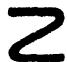
\includegraphics[keepaspectratio]{images/part001_a9a6e172.jpg}}

存在这样的非豪斯多夫空间，其中每一点都有一个豪斯多夫邻域（习题 7）。

命题 7. 豪斯多夫空间的每个积都是豪斯多夫的。反之，若非空空间的积是豪斯多夫的，则每个因子都是豪斯多夫空间。

设 \(X = \prod_{i \in I} X_i\) 是拓扑空间的一个积。于是，若 \(x, y\) 是 \(X\) 的两个不同的点，则 \(\text{pr}_i x \neq \text{pr}_i y\) 对某个指标 \(i\) 成立，而第 1 目命题 5 表明，\(X\) 是豪斯多夫的，只要诸 \(X_i\) 是豪斯多夫的。反之，若 \(X\) 是豪斯多夫的且诸 \(X_i\) 非空，则每个 \(X_i\) 同胚于 \(X\) 的一个子空间（\(\S 4\)，第 2 目，命题 4），因而是豪斯多夫的。

推论 1. 设 X 是一个集合，\((\mathbf{Y}_{\iota})_{\iota \in \mathbf{I}}\) 是豪斯多夫拓扑空间的一个族，且对每个 \(\iota \in I\)，设 \(f_{\iota}\) 是 X 到 \(Y_{\iota}\) 中的一个映射。设 X 带有最粗拓扑 \(\mathfrak{T}\)，使诸 \(f_{\iota}\) 连续。则 X 为豪斯多夫的一个必要充分条件是：对 X 的每对不同的点 x, y，\(f_{\iota}(x) \neq f_{\iota}(y)\) 对某个指标 \(\iota \in I\) 成立。

该条件依据第 1 目命题 5 是充分的。反之，设 X 是豪斯多夫的；令 \(Y = \prod_{\iota \in I} Y_{\iota}\)，并令 \(f = (f_{\iota})_{\iota \in I}\) 为映射 \(x \to (f_{\iota}(x))\)。由上面的命题 7，Y 是豪斯多夫的；又由 §4 第 1 目命题 3，\(\mathfrak{T}\) 是 Y 的拓扑在 f 下的逆像。若对 X 的两个不同的点 x, y 有 \(f(x) = f(y)\)，则显然每个（拓扑 \(\mathfrak{T}\) 中的）包含 x 的开集也包含 y，这与 X 是豪斯多夫的假设相矛盾。

推论 2. 设 \((\mathbf{X}_{\alpha}, f_{\alpha \beta})\) 是拓扑空间的一个逆系统。若诸 \(\mathbf{X}_{\alpha}\) 是豪斯多夫的，则 \(\mathbf{X} = \varprojlim \mathbf{X}_{\alpha}\) 是豪斯多夫的，并且是 \(\prod_{\alpha} \mathbf{X}_{\alpha}\) 的一个闭子空间。

第一个断言由 X 是豪斯多夫空间 \(\prod_{\alpha} X_{\alpha}\) 的子空间（命题 7）这一事实得出。为证 X 在积空间中是闭的，设 \(F_{\alpha\beta} (\alpha \leqslant \beta)\) 是 \(\prod_{\alpha} X_{\alpha}\) 中由使 \(\operatorname{pr}_{\alpha}x = f_{\alpha\beta}(\operatorname{pr}_{\beta}x)\) 的点 x 组成的子集；诸 \(F_{\alpha\beta}\) 在 \(\prod_{\alpha} X_{\alpha}\) 中是闭的（第 1 目，命题 2），因此它们的交 X 也是闭的。

显然，豪斯多夫空间的任意和（§ 2，第 4 目，例 3）都是豪斯多夫空间。

\subsection{豪斯多夫商空间}

我们来寻求使商空间 X/R 为豪斯多夫空间的条件（这时称等价关系 R 为豪斯多夫的）。首先，若 X/R 是豪斯多夫的，则 X/R 中由单点组成的诸子集是闭的（第 1 目，命题 4），因而每个模 R 的等价类在 X 中是闭的。但这个必要条件并不充分。

X/R 中开集的定义给出如下的必要充分条件：X/R 是豪斯多夫的，当且仅当 X 中任意两个不同的等价类都包含在 X 的两个不相交的饱和开子集中。我们将给出其他更便于使用的条件。

命题 8. 商空间 X/R 为豪斯多夫的一个必要条件是 R 的图象 C 在 X × X 中是闭的。若等价关系 R 是开的，则此条件也是充分的。

设 \(\varphi: X \to X/R\) 是典范映射；则 \(C\) 是 \(\varphi \times \varphi: X \times X \to (X/R) \times (X/R)\) 下对角线 \(\Delta\)（即 \((X/R) \times (X/R)\) 的对角线）的逆像。因此命题的第一部分由 \(\varphi \times \varphi\) 的连续性得出{[}公理 \((H^{ii})\) 及 §2 第 1 目定理 1{]}。若 \(R\) 是开的，则 \((X/R) \times (X/R)\) 可等同于商空间 \((X \times X)/(R \times R)\)（§5，第 3 目，命题 8 的推论），而 \(\Delta\) 这时等同于 \((X \times X)/(R \times R)\) 中集合 \(C\)（它关于 \(R \times R\) 是饱和的）的典范象。于是 \(\Delta\) 在 \(X \times X\) 中是闭的，从而 \(X\) 是豪斯多夫的。

\pandocbounded{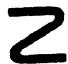
\includegraphics[keepaspectratio]{images/part001_7b053cb2.jpg}}

若 R 不是开的，则存在这样的例子：C 是闭的而 R 不是豪斯多夫的（习题 10 与 28）。

为证 X/R 是豪斯多夫的，我们也可以应用第 1 目命题 5：设 M 与 N 是 R 的两个不同的等价类，只需存在 X 的一个开子集 A 到豪斯多夫空间 \(X'\) 中的一个连续映射 f，其中 A 关于 R 饱和且包含 M 与 N，使得 1) f 在 A 所含的每个模 R 等价类上取常值，2) f 在 M 与 N 上取不同的值。因为既然 \(A/R_{A}\) 可等同于 X/R 的一个开子集（§ 3，第 6 目，命题 10，推论 1），我们就可以对由 f 诱导的映射 g: \(A/R_{A} \to X'\) 应用第 1 目命题 5，因为 g 是连续的（§ 3，第 4 目，命题 6）。

特别地：

命题 9. 若 \(f\) 是拓扑空间 \(\mathbf{X}\) 到豪斯多夫空间 \(\mathbf{X}'\) 中的一个连续映射，而 \(\mathbf{R}\) 是等价关系 \(f(x) = f(y)\)，则商空间 \(\mathbf{X} / \mathbf{R}\) 是豪斯多夫的。

命题 10. 若 X 是豪斯多夫空间，且 X 关于等价关系 R 有一个连续截面 s，则 X/R 是豪斯多夫的，且 s (X/R) 在 X 中是闭的。

因为（§ 3，第 5 目）X/R 同胚于 X 的子空间 \(s(\mathrm{X}/\mathrm{R})\)，后者是豪斯多夫的。此外，\(s(\mathrm{X}/\mathrm{R})\) 是由所有 \(x \in \mathbf{X}\) 中使 \(s(\varphi(x)) = x\) 的点组成的集合，其中 \(\varphi: \mathbf{X} \to \mathbf{X}/\mathbf{R}\) 是典范映射；因此第二个断言由第 1 目命题 2 得出。

\subsection{正则空间}

命题 11. 拓扑空间 X 的下列性质等价：

(O \(_{III}\) ) X 的任一点的诸闭邻域组成的集合是该点的一个基本邻域系。

\((O_{\mathrm{III}}^{\prime})\) 给定闭子集 \(\mathbf{F}\)（\(\mathbf{X}\) 的）与任一点 \(x \notin \mathbf{F}\)，存在 \(x\) 的一个邻域与 \(\mathbf{F}\) 的一个邻域，二者不相交。

\((\mathrm{O}_{\mathrm{III}}) \Longrightarrow (\mathrm{O}_{\mathrm{III}}^{\prime})\)：若 \(\mathbf{F}\) 是闭的且 \(x \notin \mathbf{F}\)，则存在一个闭邻域 \(\mathbf{V}\)（即 \(x\) 的闭邻域），它包含于邻域 \(\complement \mathbf{F}\)（即 \(x\) 的邻域）中；\(\mathbf{V}\) 与 \(\complement \mathbf{V}\) 分别是 \(x\) 与 \(\mathbf{F}\) 的邻域，且没有公共点。

\((\mathrm{O}_{\mathrm{III}}^{\prime}) \Longrightarrow (\mathrm{O}_{\mathrm{III}})\)：若 \(W\) 是 \(x \in X\) 的一个开邻域，则存在邻域 \(U\)（即 \(x\) 的邻域）与邻域 \(V\)（即 \(\complement W\) 的邻域），二者不相交，因此 \(\overline{U} \subset W\)。

定义 2. 拓扑空间称为正则的，如果它是豪斯多夫的且满足公理 (O \(_{III}\) )；这时它的拓扑称为正则拓扑。

离散空间是正则的。* 我们将在 § 9 中看到，每个局部紧空间（特别地，实直线 R）都是正则的。*

命题 12. 正则空间的每个子空间都是正则的。

设 A 是正则空间 X 的一个子空间。既然 X 是豪斯多夫的，A 亦然（第 2 目）；另一方面，点 \(x \in A\) 关于 A 的每个邻域都具有形状 \(V \cap A\)，其中 V 是 x 在 X 中的邻域。既然 X 是正则的，就存在 x 在 X 中的一个邻域 W，它在 X 中是闭的且包含于 V；于是 \(W \cap A\) 是 x 在 A 中的邻域，在 A 中是闭的且包含于 \(V \cap A\)。由此即得结论。反之：

命题 13. 若拓扑空间 X 的每一点 x 都有一个闭邻域，它是 X 的正则子空间，则 X 是正则的。

由第 2 目命题 6，X 是豪斯多夫的。设 x 是 X 的任一点，V 是 x 的一个闭的正则邻域。若 U 是 x 的包含于 V 中的任一邻域，则 U 是 x 关于 V 的邻域；于是由假设，存在 x 在 V 中的一个邻域 W，它在 V 中是闭的且包含于 U。但既然 V 是 x 在 X 中的邻域，W 就是 x 在 X 中的邻域；又既然 V 在 X 中是闭的，W 就在 X 中是闭的。

注. 1) 存在这样的非豪斯多夫空间，其中每一点都有一个正则邻域（习题 7）。

\begin{enumerate}
\def\labelenumi{\arabic{enumi})}
\setcounter{enumi}{1}
\item
  存在豪斯多夫但非正则的空间（习题 20）。
\item
  比正则拓扑更细的拓扑未必是正则的（习题 20）。
\end{enumerate}

\subsection{连续延拓；二重极限}

定理 1. 设 X 是一个拓扑空间，A 是 X 的一个稠密子集，\(f: \mathbf{A} \to \mathbf{Y}\) 是 A 到正则空间 Y 中的一个映射。\(f\) 可延拓为连续映射 \(\overline{f}: \mathbf{X} \to \mathbf{Y}\) 的一个必要充分条件是：对每个 \(x \in \mathbf{X}\)，\(f(y)\) 当 \(y\) 趋于 \(x\) 且保持属于 A 时在 Y 中趋于一个极限。这时连续延拓 \(\overline{f}\)（把 \(f\) 延拓到 X 上）是唯一的。

\(\vec{f}\) 的唯一性由恒等延拓原理（第 1 目，命题 2，推论 1）得出。显然该条件是必要的，因为若 \(\vec{f}\) 在 X 上连续，则对每个 \(x \in X\) 我们有

\[
\overline {{f}} (x) = \lim _ {y > x, y \in \mathbf {A}} \overline {{f}} (y) = \lim _ {y > x, y \in \mathbf {A}} f (y)
\]

（§ 7，第 5 目）。反之，设该条件成立，并定义

\[
\overline {{f}} (x) = \lim _ {y \rightarrow x, y \in \mathbf {A}} f (y)
\]

（对每个 \(x \in X\)）；\(\overline{f}(x)\) 是 Y 中一个完全确定的元素，因为 Y 是豪斯多夫的。我们必须证明 \(\overline{f}\) 在每个点 \(x \in X\) 处连续。于是设 \(V'\) 是 \(\overline{f}(x)\) 在 Y 中的一个闭邻域；则由假设，存在 x 在 X 中的一个开邻域 V，使得 \(f(V \cap A) \subset V'\)。既然 V 是它的每一点的邻域，我们就有

\[
\overline {{f}} (z) = \lim _ {y > z, y \in \mathrm{V} \cap \mathrm{A}} f (y)
\]

（对每个 \(z \in \mathbf{V}\)）；由此得出 \(\overline{f}(z) \in f(\mathbf{V} \cap \mathbf{A}) \subset \mathbf{V}'\)，因为 \(\mathbf{V}'\) 是闭的。于是结论由 \(f(x)\) 的诸闭邻域构成 \(f(x)\) 在 \(\mathbf{Y}\) 中的一个基本邻域系这一事实得出。

映射 \(\bar{f}\) 称为由 f 连续延拓到 X 上而得到的映射。

在定理 1 的陈述中，Y 是正则的这一假设不能减弱，除非对 X、A 或 f 附加额外的限制（习题 19）。

推论. 设 \(\mathfrak{F}_1\) 是集合 \(X_1\) 上的一个滤子，\(\mathfrak{F}_2\) 是集合 \(X_2\) 上的一个滤子；设 \(\mathfrak{F}_1 \times \mathfrak{F}_2\) 是 \(X = X_1 \times X_2\) 上的积滤子（§ 6，第 7 目），并设 \(f\) 是 \(X\) 到正则空间 \(Y\) 中的一个映射。假设

\begin{enumerate}
\def\labelenumi{\alph{enumi})}
\item
  \(\lim_{\mathfrak{F}_1\times \mathfrak{F}_2}f\) 存在。
\item
  \(\lim_{x_2, \mathfrak{F}_2} f(x_1, x_2) = g(x_1)\) 对所有 \(x_1 \in \mathbf{X}_1\) 存在。
\end{enumerate}

则 \(\lim_{x_1, \mathfrak{F}_1} g(x_1)\) 存在且等于 \(\lim_{\mathfrak{F}_1 \times \mathfrak{F}_2} f\)。

设 \(X_1' = X_1 \cup \{ \omega_1 \}\)（相应地，\(X_2' = X_2 \cup \{ \omega_2 \}\)）是伴随于滤子 \(\mathfrak{F}_1\)（相应地，\(\mathfrak{F}_2\)）的拓扑空间（§ 6，第 5 目，例）。在积空间 \(X' = X_1' \times X_2'\) 中，设 \(X''\) 是子空间 \(X_1 \times X_2'\) 与 \(\{ (\omega_1, \omega_2) \}\) 的并。显然 \(X\) 是 \(X''\) 的稠密子空间，且诸假设蕴含：\(f(y_1, y_2)\) 当 \((y_1, y_2)\) 趋于任一点 \((x_1, x_2)\)（在 \(X''\) 中）且保持属于 \(X\) 时趋于一个极限。于是由定理 1 得出 \(f\) 连续延拓到 \(X''\) 上的存在性。又因为 \((\omega_1, \omega_2)\) 属于 \(X_1 \times \{ \omega_2 \}\) 关于 \(X''\) 的闭包，结论立即得出（§ 7，第 5 目）。

\subsection{正则空间上的等价关系}

命题 14. 设 X 是正则空间，R 是 X 上的一个闭等价关系。则 R 在 X × X 中的图象 C 是闭的。

设 \((a, b)\) 是 \(X \times X\) 中属于 C 的闭包的一点，并设 V（相应地，W）是 \(a\) 的一个闭邻域（相应地，\(b\) 的一个邻域）；则存在一点 \((x, y) \in C \cap (V \times W)\)。既然 \(x \in V\)，\(y\) 就属于 V 关于 R 的饱和集 S；因此 \(b\) 的每个邻域 W 都与 S 相交。由假设 S 是闭的，从而 \(b \in S\)。现设 B 是 \(\{b\}\) 关于 R 的饱和集，则 \(a\) 的每个闭邻域 V 都与 B 相交；由假设 B 是闭的且 X 是正则的，由此得出 \(a \in B\)，从而 \((a, b) \in C\)。证明完毕。

推论. 在正则空间上，每个既开又闭的等价关系都是豪斯多夫的。

这由命题 14 及第 3 目命题 8 得出。

命题 15. 设 X 是正则空间，F 是 X 的一个闭子集，R 是把 F 的所有点等同起来而得到的 X 上的等价关系{[}换句话说，这个等价关系的等价类是 F（若 \(\mathbf{F} \neq \emptyset\)）以及诸集合 \(\{x\}\)，其中 \(x \in [\mathbb{C}F]\) 。则商空间 X/R 是豪斯多夫的。

设 M 与 N 是 X 中两个不同的等价类。若它们各由 F 的余集中的单点组成，则在豪斯多夫子空间 \(\complement F\) 中存在 M 与 N 的两个不相交的开邻域；它们是 M 与 N 在 X 中的邻域，且关于 R 饱和。若 M = F（于是 \(F \neq \varnothing\)）而 \(N = \{b\}\)，其中 \(b \notin F\)，则既然 X 是正则的，就存在 b 的一个开邻域与 F 的一个开邻域，二者不相交；这些邻域关于 R 饱和，命题得证。

注意，商空间 X/R 未必是正则的（第九章，§ 4，习题 14）。

\section{紧空间与局部紧空间}

\subsection{拟紧空间与紧空间}

定义 1. 拓扑空间 X 称为拟紧的，如果它满足以下公理：

\begin{enumerate}
\def\labelenumi{(\Alph{enumi})}
\setcounter{enumi}{2}
\tightlist
\item
  X 上的每个滤子都至少有一个聚点。
\end{enumerate}

拓扑空间称为紧的，如果它既是拟紧的又是豪斯多夫的。

由这个公理立即得出：若 \(f\) 是集合 \(Z\) 到拟紧空间 \(X\) 中的一个映射，而 \(\mathfrak{F}\) 是 \(Z\) 上的任一滤子，则 \(f\) 关于 \(\mathfrak{F}\) 至少有一个聚点。特别地，拟紧空间的每个点列都至少有一个聚点；但这个条件并不等价于 (C)（习题 11）。

我们给出三个公理，其中每一个都等价于公理 (C)：

(C') \(X\) 上的每个超滤子都收敛。

\((\mathrm{C}^{\prime}) \Longrightarrow (\mathrm{C})\)：若 \(\mathfrak{F}\) 是 \(\mathbf{X}\) 上的一个滤子，则存在比 \(\mathfrak{F}\) 更细的超滤子（§ 6，第 4 目，定理 1）。既然这个超滤子收敛于一点 \(x\)，\(x\) 就是 \(\mathfrak{F}\) 的聚点。

\begin{enumerate}
\def\labelenumi{(\Alph{enumi})}
\setcounter{enumi}{2}
\tightlist
\item
  \(\Longrightarrow\) (C')：因为若一个超滤子有一个聚点，则它收敛于该点（§ 7，第 2 目，命题 4 的推论）。
\end{enumerate}

若 \(f\) 是集合 \(Z\) 到拟紧空间 \(X\) 中的一个映射，而 \(\mathfrak{U}\) 是 \(Z\) 上的一个超滤子，则 \(f\) 关于 \(\mathfrak{U}\) 至少有一个极限点（§ 6，第 6 目，命题 10）。

(C'') X 的闭子集的每个交为空的族都包含一个交为空的有限子族。

\begin{enumerate}
\def\labelenumi{(\Alph{enumi})}
\setcounter{enumi}{2}
\tightlist
\item
  \(\Longrightarrow\) (C'\,')：设 \(\mathfrak{G}\) 是 X 的闭子集的一个交为空的族。若 \(\mathfrak{G}\) 的每个有限子族都有非空的交，则 \(\mathfrak{G}\) 生成一个滤子（§ 6，第 2 目，命题 1），由假设它有一个聚点。这个点属于 \(\mathfrak{G}\) 的所有集合（因为它们是闭的）；于是得到矛盾。
\end{enumerate}

\((\mathbf{C}^{\prime\prime}) \Longrightarrow (\mathbf{C}) : \text{因为若 } (\mathbf{C}) \text{为假，则存在一个滤子 } \mathfrak{F} \text{在 } \mathbf{X} \text{上没有聚点；因此滤子 } \mathfrak{F} \text{中的各集合的闭包构成 } \mathbf{X} \text{的一个闭子集族，违背公理 } (\mathbf{C}^{\prime\prime}).\)

(C \(^{iii}\) )（Borel-Lebesgue 公理）X 的每个开覆盖都包含 X 的一个有限开覆盖。

\((\mathbf{C}^{\prime\prime\prime}) \iff (\mathbf{C}^{\prime\prime})\)，取余集即得。

若 X 是拟紧的，则 X 的每个局部有限覆盖 R 都是有限的。因为 X 的每一点都有一个只与 R 中有限多个集合相交的开邻域，而由 \((\mathbf{C}^{\prime\prime})\)，这些邻域中的有限多个覆盖 X。

例. 1) 每个有限空间都是拟紧的，更一般地，每个只含有限多个开集的空间都是拟紧的。有限空间是紧的当且仅当它是离散的，因为有限豪斯多夫空间是离散的（§ 8，第 1 目，命题 3 的推论）。反之，每个紧的离散空间都是有限的，因为在这种空间中由单点组成的诸集合都是开集；于是由 (C'\,')，该空间是有限的。

\begin{enumerate}
\def\labelenumi{\arabic{enumi})}
\setcounter{enumi}{1}
\tightlist
\item
  设 X 是一个集合，给 X 赋以这样的拓扑：其闭集为 X 及 X 的所有有限子集{[}这个子集族显然满足 §1 第 4 目的公理 \((\mathrm{O}_{\mathrm{I}}^{\prime})\) 与 \((\mathrm{O}_{\mathrm{II}}^{\prime})\){]}。这样定义的拓扑空间是拟紧的。因为若 \((\mathbf{F}_{i})_{i\in I}\) 是 X 的闭子集的一个交为空的族，则 \(F_{\alpha}\) 对某个 \(\alpha\in I\) 是有限的。设 \(a_{k}\)（\(1\leqslant k\leqslant n\)）是 \(F_{\alpha}\) 的诸元素；则由假设，对每个指标 k 存在指标 \(i_{k}\in I\) 使 \(a_{k}\notin F_{i_{k}}\)；于是诸 \(F_{i_{k}}\)（\(1\leqslant k\leqslant n\)）与 \(F_{\alpha}\) 的交为空，从而公理 \((\mathrm{C}^{\prime\prime})\) 得以满足。若 X 是无限集，它就不是豪斯多夫的。
\end{enumerate}

注. 拟紧（非豪斯多夫）空间主要用于拓扑学对代数几何的应用，很少出现在其他数学理论中；与之相反，紧空间在其他数学理论中扮演着重要角色。

定理 1. 设 \(\mathfrak{F}\) 是拟紧空间 \(\mathbf{X}\) 上的一个滤子，并设 \(\mathbf{A}\) 是 \(\mathfrak{F}\) 的聚点组成的集合。则 \(\mathbf{A}\) 的每个邻域都属于 \(\mathfrak{F}\)。

设 V 是 A 的一个邻域，并假设 F 的每个集合都与 CV 相交。于是 F 的诸集合与 CV 的交构成 X 上一个滤子 G 的基；X 是拟紧的，故 G 至少有一个聚点 y，而 y 不属于 A，因为 A 的邻域 V 不与 G 的某些集合相交。但既然 G 比 F 更细，y 也是 F 的聚点，这与假设矛盾。

推论. 紧空间上的一个滤子收敛，当且仅当它只有一个聚点。

必要性由 § 8，第 1 目，命题 1 得出；充分性由上面的定理 1 得出。

\subsection{紧空间的正则性}

命题 I. 设 X 是紧空间，x 是 X 的一点。为使由 x 的闭邻域组成的一个滤子基 B 是 x 的基本邻域系，必要且充分的是 B 中诸集合之交仅由 x 组成。

该条件是必要的，因为 X 是豪斯多夫的（§ 8，第 1 目，命题 1）。它也是充分的，因为它意味着 x 是 B 的唯一聚点；于是由第 1 目定理 1 的推论，B 收敛于 x。

推论. 每个紧空间都是正则的。

因为由公理 (Hi)（§ 8，第 1 目，命题 1），由该空间任一点的所有闭邻域组成的滤子基满足命题 I 的条件。

下面的命题加强了命题 I 的推论：

命题 2. 设 X 是紧空间，并设 A, B 是 X 的两个不相交的闭子集。则存在两个开集 U, V，使得 \(U \cap V = \varnothing\) 且 \(A \subset U\) 且 \(B \subset V\)。

设结论不真。若 A 的每个邻域 U 都与 B 的每个邻域 V 相交，则诸集合 \(U \cap V\) 在 X 上构成一个滤子基 B，从而它有一个聚点 \(x \in X\)。现在 x 必属于 A，因为若 y 是 X 中不属于 A 的任一点，则由于 X 是正则的，存在 y 的一个邻域与 A 的一个邻域，二者不相交，从而 y 不可能是 B 的聚点。类似地，x 必属于 B，于是得到矛盾。

\pandocbounded{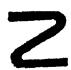
\includegraphics[keepaspectratio]{images/part001_de955d1b.jpg}}

这个命题有重要的推论，将在第九章 § 4 中考察。

第 1 目例 2 中的非豪斯多夫拟紧空间 X 既不满足公理 (O \(_{III}\) )，更不满足命题 2 所述的性质，因为这个空间的任意两个非空开集总相交。

\subsection{拟紧集；紧集；相对紧集}

定义 2. 拓扑空间 X 的子集 A 称为拟紧集（相应地，紧集），如果子空间 A 是拟紧的（相应地，紧的）。

拓扑空间 X 的子集 A 是拟紧集，当且仅当每个由 X 的开集组成的 A 的覆盖都包含 A 的一个有限覆盖；这由公理 (C'\,') 得出。在豪斯多夫空间中，拟紧集与紧集这两个概念相同，因为每个子空间都是豪斯多夫的。

例. 1) 在拓扑空间 X 中，每个有限子集都是拟紧的；空集与每个单点集都是紧的。2) 在拓扑空间 X 中，设 \((x_{n})_{n\in \mathbb{N}}\) 是收敛于一点 \(a\) 的一个无穷点列；则由诸点 \(x_{n}\)（\(n\in \mathbb{N}\)）与 \(a\) 组成的集合 A 是拟紧的。因为若 \((\mathrm{U}_{\iota})\) 是由 X 的开集组成的 A 的一个覆盖，则 \(a\in \mathrm{U}_{\iota}\) 对某个指标 \(\iota\) 成立。\(\mathrm{U}_{\iota}\) 是 \(a\) 的邻域，因此只有有限多个指标 \(n_k\) 使 \(x_{nk}\notin \mathrm{U}_{\iota}\)。对每个指标 \(k\)，设 \(\iota_{k}\) 是使 \(x_{nk}\in \mathrm{U}_{\iota_{k}}\) 的一个指标；则 \(\mathrm{U}_{\iota}\) 与诸 \(\mathrm{U}_{\iota_{k}}\) 构成 A 的一个有限开覆盖。

命题 3. 拟紧（相应地，紧）空间的每个闭子集都是拟紧（相应地，紧）的。

只要注意到：若 A 在 X 中是闭的，则在 A 中闭的每个集合在 X 中也是闭的，这便是公理 (C'') 的直接推论。

命题 4. 豪斯多夫空间的每个紧子集都是闭的。

设 A 是豪斯多夫空间 X 的一个紧子集，并设 x 是 \(\overline{A}\) 的任一点；我们要证明 \(x \in A\)。由假设，x 的每个邻域都与 A 相交，因此 x 在 X 中的邻域滤子 B 在 A 上诱导一个滤子 \(B_{A}\)；A 是紧的，故 \(B_{A}\) 有一个聚点 \(y \in A\)。既然滤子 B 比 \(B_{A}\)（视为 X 上的一个滤子基）在 X 上生成的滤子更粗，y 也是 B 的聚点；于是 y = x，因为 B 在 X 中收敛于 x，且 X 是豪斯多夫的（§ 8，第 1 目，命题 1）。

推论. 在紧空间 X 中，子集 A 是紧的，当且仅当它在 X 中是闭的。

命题 5. 拓扑空间中拟紧子集的一个有限族的并是拟紧的。

只需证明：若 A 与 B 是拓扑空间 X 的两个拟紧子集，则 \(A \cup B\) 是拟紧的。设 R 是 \(A \cup B\) 的一个覆盖；则 R 既是 A 的覆盖又是 B 的覆盖；于是 R 包含 A 的一个有限覆盖 \(R_{1}\) 与 B 的一个有限覆盖 \(R_{2}\)；从而 \(R_{1} \cup R_{2}\) 是 \(A \cup B\) 的一个包含于 R 中的有限覆盖。

定义 3. 拓扑空间 X 的子集 A 称为 X 中相对拟紧（相应地，相对紧）的，如果 A 包含于 X 的一个拟紧（相应地，紧）子集之中。

为简便起见，当关于 X 没有歧义时，我们也说 A 是“相对拟紧集”（相应地，“相对紧集”）。在豪斯多夫空间中，相对拟紧集与相对紧集这两个概念相同。

命题 6. 若 X 是豪斯多夫空间，则 X 的子集 A 是相对紧的，当且仅当 \(\overline{A}\) 是紧的。

若 A 是相对紧的，则由命题 4 及其推论，\(\overline{A}\) 是紧的；反向的蕴含是显而易见的。

命题 7. 若 A 是拓扑空间 X 的一个相对拟紧子集，则 A 上的每个滤子基在 X 中都有一个聚点。

因为若 \(\mathbf{A} \subset \mathbf{K}\)，其中 \(\mathbf{K}\) 是 \(\mathbf{X}\) 的一个拟紧子集，则 \(\mathbf{A}\) 上的每个滤子基在 \(\mathbf{K}\) 中都有一个聚点。

这个命题的逆命题在对 X 不加限制时并不成立（习题 22）。

\pandocbounded{
\includegraphics[keepaspectratio]{images/part001_f875b0ae.jpg}}

注. 在非豪斯多夫空间中，紧集未必是闭的，其闭包也未必是拟紧的（习题 5）；两个紧集的交未必是拟紧的（习题 5）；两个紧集的并未必是紧的（习题 5）。

\subsection{紧空间在连续映射下的象}

定理 2. 若 \(f\) 是拟紧空间 \(\mathbf{X}\) 到拓扑空间 \(\mathbf{X}'\) 中的一个连续映射，则集合 \(f(\mathbf{X})\) 是拟紧的。

设 \(\Re\) 是 \(f(\mathbf{X})\) 的一个由 \(\mathbf{X}'\) 中开集组成的覆盖；则 \(\overline{f}^{1}(\Re)\) 是 \(\mathbf{X}\) 的一个开覆盖（\(\S 2\)，第 1 目，定理 1）；于是存在有限子集 \(\mathfrak{S}\)（\(\Re\) 的），使 \((\mathfrak{S}\overline{f}^{1})\) 是 \(\mathbf{X}\) 的一个覆盖；但这时 \(\mathfrak{S}\) 就是 \(f(\mathbf{X})\) 的一个覆盖，定理得证。

推论 1. 设 \(f\) 是拓扑空间 \(\mathbf{X}\) 到豪斯多夫空间 \(\mathbf{X}'\) 中的一个连续映射。则在 \(f\) 之下，\(\mathbf{X}\) 中任一拟紧（相应地，相对拟紧）集的象是 \(\mathbf{X}'\) 中的一个紧（相应地，相对紧）集。

推论 2. 每个连续映射 \(f\)（拟紧空间 \(X\) 到豪斯多夫空间 \(X'\) 中的）都是闭映射。若此外 \(f\) 还是双射，则 \(f\) 是一个同胚。

这由第 3 目的推论 1 与命题 4 立即得出。

特别地：

推论 3. 比拟紧空间的拓扑更粗的豪斯多夫拓扑必与后者一致。

推论 4. 设 X 是一个拓扑空间，R 是 X 上的一个豪斯多夫等价关系。

\begin{enumerate}
\def\labelenumi{\alph{enumi})}
\item
  若 X 中存在一个与每个模 R 等价类都相交的拟紧集 K，则 X/R 是紧的，且 \(K/R_{K}\) 到 X/R 上的典范映射是一个同胚。
\item
  若 K 与每个等价类还只交于一点，则 K 是 X 关于关系 R 的一个连续截面（§ 3，第 5 目）。
\end{enumerate}

设 \(f\) 是限制到 \(K\) 上的典范映射 \(X \to X / R\)。既然 \(X / R\) 是豪斯多夫的，由推论 1 得出 \(X / R\) 是紧的；又由推论 2 得出 \(f\) 是闭映射；于是双射 \(K / R_K \to X / R\)（伴随于 \(f\)）是一个同胚（§ 5，第 2 目，命题 3）。这就处理了 a)；b) 立即得出，因为这时有 \(K / R_K = K\)。

\subsection{紧空间的积}

定理 3（Tychonoff）. 拟紧（相应地，紧）空间的每个积都是拟紧（相应地，紧）的。反之，若非空空间的积是拟紧（相应地，紧）的，则每个因子都是拟紧（相应地，紧）的。

鉴于 § 8 第 2 目命题 7 给出的豪斯多夫积空间的刻画，只需对拟紧空间证明这些断言。若 \(\mathbf{X} = \prod_{\iota \in I} \mathbf{X}_{\iota}\) 是拟紧的且非空，则由第 4 目定理 2，\(\mathbf{X}_{\iota}=\mathrm{pr}_{\iota}(\mathbf{X})\) 是拟紧的。反之，设诸 \(X_{\iota}\) 是拟紧的，并设 U 是 X 上的一个超滤子；则对每个 \(\iota\in I\)，\(\mathrm{pr}_{\iota}(\mathfrak{U})\) 是 \(X_{\iota}\) 上的一个超滤子基（§ 6，第 6 目，命题 10），由公理 (C') 它收敛；于是 U 收敛（§ 7，第 6 目，命题 10 的推论 1），因此 X 是拟紧的。

推论. 拓扑空间之积的一个子集是相对拟紧的，必要且充分的是，它的每个投影在相应的因子中都是相对拟紧的。

必要性由 § 4 定理 2 得出。为证充分性，设 A 是 \(\prod_{i} X_{i}\) 的一个子集，使得对每个指标 \(i\)，\(\operatorname{pr}_{i}(A)\) 包含于拟紧子集 \(K_{i}\)（\(X_{i}\) 的）中；则 A 包含于拟紧子集 \(\prod_{i} K_{i}\)（\(\prod_{i} X_{i}\) 的）中。

\subsection{紧空间的逆极限}

命题 8. 设 \((\mathbf{X}_{\alpha}, f_{\alpha \beta})\) 是由有向集 I 加标的紧空间的一个逆系统，使得 \(f_{\alpha \alpha}\) 对每个 \(\alpha \in \mathbf{I}\) 是恒同映射。设 \(\mathbf{X} = \varprojlim \mathbf{X}_{\alpha}\) 是逆极限，\(f_{\alpha}: \mathbf{X} \to \mathbf{X}_{\alpha}\) 是典范映射（§ 4，第 4 目）。则

\begin{enumerate}
\def\labelenumi{\alph{enumi})}
\tightlist
\item
  X 是紧的，且对每个 \(\alpha \in I\) 我们有
\end{enumerate}

\[
f _ {\alpha} (\mathbf {X}) = \bigcap_ {\beta \geqslant \alpha} f _ {\alpha \beta} (\mathbf {X} _ {\beta}).\tag{I}
\]

\begin{enumerate}
\def\labelenumi{\alph{enumi})}
\setcounter{enumi}{1}
\tightlist
\item
  若诸 \(\mathbf{X}_{\alpha}\) 都非空，则 \(\mathbf{X}\) 非空。
\end{enumerate}

X 是 \(\prod_{\alpha} X_{\alpha}\) 的一个闭子空间（§ 8，第 2 目，命题 7，推论 2）

而后者由第 5 目定理 3 与第 3 目命题 3 是紧的。其余断言是《集合论》第三章 § 7 第 4 目定理 1 的推论。我们应用这个定理时，取 \(\mathfrak{S}_{\alpha}\) 为 \(\mathbf{X}_{\alpha}\) 的闭子集组成的集合。条件 (i) 与 (ii) 分别就是公理 \((\mathrm{O}_{\mathbf{i}}^{\prime})\) 与 \((\mathbf{C}^{\prime \prime})\)；条件 (iii) 得以满足，因为 \(\{x_{\alpha}\}\) 是闭的且 \(f_{\alpha \beta}\) 连续（\(\S 2\)，第 1 目，定理 1）；最后，条件 (iv) 由第 4 目定理 2 的推论 2 得以满足。

推论 1. 设 \((\mathbf{X}_{\alpha}, f_{\alpha\beta})\) 是由一个有向集加标的拓扑空间的逆系统，使得对每对指标 \(\alpha\), \(\beta\)（满足 \(\alpha \leqslant \beta\)）及每个 \(x_{\alpha} \in X_{\alpha}\)，\(\overline{f}_{\alpha\beta}(x_{\alpha})\) 是紧的。则等式 (1) 成立，且 \(\overline{f}_{\alpha}(x_{\alpha})\) 对每个 \(\alpha\) 与每个 \(x_{\alpha} \in X_{\alpha}\) 是紧的。

对每个 \(x_{\alpha} \in \bigcap_{\beta \geqslant \alpha} f_{\alpha \beta}(X_{\beta})\) 及每个 \(\beta \geqslant \alpha\)，令 \(L_{\beta}\) 表示 \(\overline{f}_{\alpha \beta}^{1}(x_{\alpha})\)。若 \(\alpha \leqslant \beta \leqslant \gamma\)，则我们有 \(f_{\beta \gamma}(L_{\gamma}) \subset L_{\beta}\)，且满足 \(\beta \geqslant \alpha\) 的全体指标组成的集合在指标集中是共尾的。由此立即得出，诸 \(L_{\beta} (\beta \geqslant \alpha)\) 构成拓扑空间的一个逆系统（以诸 \(f_{\beta \gamma}\) 的限制为映射），其逆极限 \(L\) 同胚于 \(\overline{f}_{\alpha}^{1}(x_{\alpha})\)。既然由假设诸 \(L_{\beta}\) 是紧的且非空，该推论由命题 8 得出。

推论 2. 设 \((\mathbf{X}_{\alpha}, f_{\alpha \beta})\) 与 \((\mathbf{X}_{\alpha}^{\prime}, f_{\alpha \beta}^{\prime})\) 是由同一有向集 I 加标的拓扑空间的两个逆系统，并设 \((u_{\alpha})\) 是映射 \(u_{\alpha}: \mathbf{X}_{\alpha} \to \mathbf{X}_{\alpha}^{\prime}\) 的一个逆系统。设 \(\mathbf{X} = \varprojlim \mathbf{X}_{\alpha}\)，\(\mathbf{X}^{\prime} = \varprojlim \mathbf{X}_{\alpha}^{\prime}\)，\(u = \varprojlim u_{\alpha}\)。则：

\begin{enumerate}
\def\labelenumi{\alph{enumi})}
\item
  若 \(x' = (x_{\alpha}') \in \mathbf{X}'\) 使 \(\overline{u}_{\alpha}(x_{\alpha}')\) 对每个 \(\alpha \in I\) 是紧的且非空，则 \(\overline{u}^1(x')\) 是紧的且非空。
\item
  若诸 \(X_{\alpha}\) 是紧的，诸 \(X_{\alpha}^{\prime}\) 是豪斯多夫的，且诸 \(u_{\alpha}\) 是满射与连续的，则 u 是满射。
\end{enumerate}

令 \(\mathbf{L}_{\alpha}\) 表示 \(\overline{\boldsymbol{u}}_{\alpha}^{1}(x_{\alpha}^{\prime})\)；则显然诸 \(\mathbf{L}_{\alpha}\) 构成拓扑空间的一个逆系统（以诸 \(f_{\alpha \beta}\) 的限制为映射），且 \(\overline{\boldsymbol{u}}^{1}(x^{\prime} = \mathbf{L})\) 是诸 \(\mathbf{L}_{\alpha}\) 的逆极限；因此断言 a) 由命题 8 得出。鉴于第 3 目命题 3，断言 b) 是一个直接推论。

\subsection{局部紧空间}

定义 4. 拓扑空间 X 称为局部紧的，如果它是豪斯多夫的且 X 的每一点都有一个紧邻域。

显然紧空间是局部紧的，但反之不真；例如，每个离散空间都是局部紧的，但若是无限的则不是紧的。

* 我们将在第四章 § 2 中看到，实直线 R 是局部紧的，但不是紧的。*

命题 9. 每个局部紧空间都是正则的。

设 X 是局部紧空间，则每点 \(x \in X\) 都有一个紧邻域 V；既然 X 是豪斯多夫的，V 是闭的（第 3 目，命题 4）。另一方面，V 是 X 的正则子空间（第 2 目，命题 1 的推论），因此 X 是正则的（§ 8，第 4 目，命题 13）。

推论. 在局部紧空间中，每一点都有一个紧邻域组成的基本邻域系。

因为 x 的一个闭邻域与 x 的一个紧邻域之交是 x 的一个紧邻域（第 3 目，命题 3）。

\pandocbounded{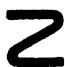
\includegraphics[keepaspectratio]{images/part001_13daf5c9.jpg}}

存在这样的非豪斯多夫拓扑空间，其中每一点都有一个由紧邻域组成的基本邻域系（习题 5）。

命题 9 的推论可以如下推广：

命题 10. 在局部紧空间 X 中，每个紧集 K 都有一个由紧邻域组成的基本邻域系。

设 \(\mathbf{U}\) 是 \(\mathbf{K}\) 的任一邻域。对每个 \(x \in \mathbf{K}\)，存在紧邻域 \(\mathbf{W}(x)\)（即 \(x\) 的紧邻域），它包含于 \(\mathbf{U}\)。当 x 跑遍 K 时，诸集合

W (x) 的内部构成 K 的一个开覆盖；于是存在有限多个点 \(x_{i} \in K\)（\(1 \leqslant i \leqslant n\)），使诸 \(W(x_{i})\) 的内部覆盖 K。因此诸 \(W(x_{i})\) 的并 V 是 K 的一个包含于 U 中的紧邻域（第 3 目，命题 5）。

命题 11. 设 X 是局部紧空间，F 是 X 的一个子集，使得每当 K 是 X 的紧子集时 \(F \cap K\) 都是紧的。则 F 在 X 中是闭的。

鉴于第 3 目命题 4，这由 § 3 第 1 目命题 3 a) 得出。

命题 12. 在豪斯多夫空间 X 中，每个局部紧子空间 A 都是局部闭的。

由假设，对每个 \(x \in A\)，存在 x 在 X 中的一个邻域 V，使得 \(V \cap A\) 是紧的，从而在 V 中是闭的（第 3 目，命题 4）。

命题 13. 局部紧空间 X 的每个局部闭子空间都是局部紧的。

设 A 是 X 的一个局部闭子空间；则对每个 \(x \in A\)，存在 x 在 X 中的一个邻域 U，使得 \(U \cap A\) 在 U 中是闭的。设 \(V \subset U\) 是 x 在 X 中的一个紧邻域；\(V \cap A = V \cap (U \cap A)\) 在 V 中是闭的，从而是紧的（第 3 目，命题 3）。既然 \(V \cap A\) 是 x 在 A 中的一个邻域，结论得证（显然 A 是豪斯多夫的）。

\pandocbounded{
\includegraphics[keepaspectratio]{images/part001_5df2d3a1.jpg}}

定理 1（第 1 目）与定理 2 的推论 2（第 4 目）不能推广到非紧的局部紧空间。

例如，在无限离散空间 X 中，由包含给定点 \(x \in X\) 且余集有限的那些集合组成的滤子以 x 为唯一聚点，但不收敛于 x。既然 X 到豪斯多夫空间 \(X'\) 中的任何映射 f 都连续，f 之下 X 的任一子集（因 X 是离散的，它在 X 中是闭的）的象一般不是 \(X'\) 的闭子集。

与第 5 目定理 3 相应的命题如下：

命题 14. a) 设 \((\mathbf{X}_{\iota})_{\iota \in I}\) 是局部紧空间的一个族，使得除有限多个指标外 \(\mathbf{X}_{\iota}\) 都是紧的。则积空间 \(\mathbf{X} = \prod_{\iota \in I} \mathbf{X}_{\iota}\) 是局部紧的。

\begin{enumerate}
\def\labelenumi{\alph{enumi})}
\setcounter{enumi}{1}
\item
  反之，若非空拓扑空间的族 \((\mathbf{X}_{\iota})_{\iota\in I}\) 的积是局部紧的，则除有限多个指标外诸因子 \(\mathbf{X}_{\iota}\) 都是紧的，且不紧的那些因子是局部紧的。
\item
  设 \(x = (x_{\iota})\) 是 \(X\) 的一点。对每个指标 \(\iota \in I\)，若 \(X_{\iota}\) 局部紧但不紧，则设 \(V_{\iota}\) 是 \(x_{\iota}\) 在 \(X_{\iota}\) 中的一个紧邻域，而对所有其他指标 \(\iota\) 令 \(V_{\iota} = X_{\iota}\)。则 \(\prod_{\iota \in I} V_{\iota}\) 是 \(x\) 在 \(X\) 中的一个紧邻域（第 5 目，定理 3）。又由 § 8 第 2 目命题 7，\(X\) 是豪斯多夫的，从而是局部紧的。
\item
  若 \(X = \prod_{\iota \in I} X_{\iota}\) 是局部紧的且诸 \(X_{\iota}\) 非空，则每个 \(X_{\iota}\) 同胚于 \(X\) 的一个闭子空间（§ 4，第 2 目，命题 4 及 § 4，第 3 目，命题 7 的推论），于是由命题 13 是局部紧的。设 \(a = (a_{\iota})\) 是 \(X\) 的一点，\(V\) 是 \(a\) 的一个紧邻域；既然除有限多个指标外我们有 \(pr_{\iota}V = X_{\iota}\)（§ 4，第 1 目），则由第 4 目定理 2 的推论 1，除有限多个指标外诸 \(X_{\iota}\) 都是紧的。
\end{enumerate}

\subsection{局部紧空间在紧空间中的嵌入}

定理 4（Alexandroff）. 若 X 是任一局部紧空间，则存在一个紧空间 \(X'\) 以及 X 到 \(X'\) 中一点的余集上的一个同胚 f。此外，设 \(X_{1}'\) 是另一个紧空间，且存在一个同胚 \(f_{1}\) 把 X 映到 \(X_{1}'\) 中一点的余集上，则存在 \(X'\) 到 \(X_{1}'\) 上的唯一一个同胚 g，使得 \(f_{1}=g\circ f\)。

我们先证明定理的第二个断言。设

\[
f (\mathbf {X}) = \mathbf {X} ^ {\prime} - \left\{\omega \right\} \quad \text { and } \quad f _ {1} (\mathbf {X}) = \mathbf {X} _ {1} ^ {\prime} - \left\{\omega_ {1} \right\}.
\]

若同胚 \(g\) 存在，它必是唯一的，因为按定义有 \(g(x') = f_1(\overline{f}^1 (x'))\)（只要 \(x' \neq \omega\)），从而 \(g(\omega) = \omega_1\)。尚须证明这样定义的双射 \(g: \mathbf{X}' \to \mathbf{X}_1'\) 是双连续的；既然 \(\mathbf{X}'\) 与 \(\mathbf{X}_1'\) 可以互换，我们只需证明 \(g\) 之下点 \(x' \in \mathbf{X}'\) 的一个邻域的象是 \(g(x')\) 在 \(\mathbf{X}_1'\) 中的一个邻域。这由 \(g\) 的定义当 \(x' \neq \omega\) 时是显然的。若 \(x' = \omega\)，设 \(V'\) 是 \(\omega\) 在 \(X'\) 中的一个开邻域；则 \(X' - V' = K\) 在 \(X'\) 中是闭的，从而是紧的（第 3 目，命题 3），且包含于 \(f(X)\)；于是 \(g(K) = f_1(\overline{f}^1 (K))\) 是紧的（第 4 目，定理 2，推论 1）。由此得出 \(g(V') = X_1' - g(K)\) 是 \(\omega_1\) 的一个开邻域（第 3 目，命题 4）。因此 \(g\) 是一个同胚。

为证明定理的第一部分，设 \(X'\) 是这样一个集合：它是 X 与由单点 \(\omega\) 组成的集合之和。我们这样在 \(X'\) 上定义一个拓扑：取 \(X'\) 的开集组成的集合 D 由 X 的所有开集以及所有形如 \((\mathbf{X}-\mathbf{K})\cup\{\omega\}\) 的子集组成，其中 K 是 X 的一个紧子集。既然 X 的紧子集的任意交是紧的（第 3 目，命题 3 与命题 4），且紧集的任意闭子集是紧的（第 3 目，命题 3），由此得出 \(\mathfrak{D}\) 满足公理 \((\mathrm{O_I})\)；又既然 X 的紧子集的任意有限并是紧的（第 3 目，命题 5），\(\mathfrak{D}\) 也满足 \((\mathrm{O_{II}})\)。X 的每个紧子集在 X 中是闭的（第 3 目，命题 4），因此 \(\mathbf{X}'\) 的拓扑在 X 上诱导的拓扑就是 X 上原有的拓扑。于是尚须证明 \(\mathbf{X}'\) 是紧的。首先，\(\mathbf{X}'\) 是豪斯多夫的。因为若 \(x, y\) 是 X 的任意两个不同的点，它们在 X 中分别有不相交的开邻域 V, W，而 V, W 在 \(\mathbf{X}'\) 中是开的；另一方面，每个 \(x \in \mathbf{X}\) 在 X 中有一个紧邻域 K，它也是 \(x\) 在 \(\mathbf{X}'\) 中的邻域，而

\[
(\mathbf {X} - \mathbf {K}) \cup \{\omega \}
\]

是 \(\omega\) 在 \(\mathbf{X}'\) 中的一个邻域，且显然不与 \(\mathbf{K}\) 相交。最后，\(\mathbf{X}'\) 是拟紧的。设 \((\mathbf{U}_{\lambda})_{\lambda \in \mathbf{L}}\) 是 \(\mathbf{X}'\) 的一个开覆盖；则至少对一个指标 \(\mu \in \mathbf{L}\) 有 \(\mathbf{U}_{\mu} = (\mathbf{X} - \mathbf{K}_{\mu}) \cup \{\omega\}\)，其中 \(\mathbf{K}_{\mu}\) 是 \(\mathbf{X}\) 的一个紧子集。于是存在有限子集 \(\mathbf{H}\)（\(\mathbf{L}\) 的），使得诸集合 \(\mathbf{U}_{\lambda}\)（\(\lambda \in \mathbf{H}\)）覆盖 \(\mathbf{K}_{\mu}\)；若 \(\mathbf{J} = \mathbf{H} \cup \{\mu\}\)，则 \((\mathbf{U}_{\lambda})_{\lambda \in \mathbf{J}}\) 是 \(\mathbf{X}'\) 的一个有限开覆盖，证明完毕。

注意，若 X 已经是紧的，则 \(\omega\) 是紧空间 \(X'\) 的一个孤立点；故 \(X'\)（\(\S\) 2，第 4 目，例 3）是空间 X 与空间 \(\{\omega\}\) 的和。

当紧空间 \(X'\) 已如上从局部紧空间 X 添加一个元素 \(\omega\) 而构造出来时，常说 \(\omega\) 是 \(X'\) 的“无穷远点”，并说 \(X'\) 是由 X 添加一个无穷远点而得到的。\(X'\) 也称为局部紧空间 X 的 Alexandroff 紧化或单点紧化。

* 例. 若把 Alexandroff 定理应用于实平面 \(\mathbf{R}^2\)，我们就得到一个紧空间，它同胚于球面 \(\mathbf{S}_2\)，其方程为 \(x_1^2 + x_2^2 + x_3^2 = 1\)（在 \(\mathbf{R}^3\) 中）。这两个空间之间的一个同胚可描述如下：点 \(\omega\)（无穷远点，添加于 \(\mathbf{R}^2\)）映到 \((0, 0, 1) \in \mathbf{S}_2\)，而每个点 \((x_1, x_2)\)（\(\mathbf{R}^2\) 的）映到连接点 \((0, 1, 1)\) 与 \((x_1, x_2, 0)\) 的直线（在 \(\mathbf{R}^3\) 中）与 \(\mathbf{S}_2\) 的另一个交点。这个同胚称为球极投影。

\subsection{局部紧 σ 紧空间}

定义 5. 局部紧空间 X 称为 σ 紧的或无穷远处可数的，如果它是紧子集的一个可数并。

例. 1) 离散空间是 \(\sigma\) 紧的当且仅当它是可数的。*2) 实直线 \(\mathbf{R}\) 是局部紧且 \(\sigma\) 紧的，因为它是诸紧区间 \([-n, +n]\)（\(n \in \mathbb{N}\)）的并。*

\pandocbounded{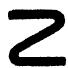
\includegraphics[keepaspectratio]{images/part001_9ca68205.jpg}}

注. 豪斯多夫空间可以是紧子空间的可数并而不是局部紧的。* 例如带弱拓扑的 Hilbert 空间便是如此，我们将在后续卷中证明这一点。

命题 15. 若 X 是局部紧 \(\sigma\) 紧空间，则存在 X 的相对紧开子集的一个序列 \((\mathbf{U}_n)\)，它覆盖 X，且 \(\overline{\mathbf{U}}_n \subset \mathbf{U}_{n+1}\) 对每个 \(n\) 成立。

设 X 是紧集序列 \((\mathbf{K}_{n})\) 的并。设 \(U_{1}\) 是 \(K_{1}\) 的一个相对紧开邻域（第 7 目，命题 10），并归纳地定义 \(U_{n}\)（对 n \textgreater{} 1）为 \(\overline{U}_{n-1} \in K_{n}\) 的一个相对紧开邻域（第 3 目，命题 5；第 7 目，命题 10）。序列 \((\mathbf{U}_{n})\) 显然具有所需的性质。

推论 1. 用命题 15 的记号，X 的每个紧子集 K 都包含于某个 \(U_{n}\) 中。

因为 K 可由有限多个 \(U_{k}\) 覆盖，依据公理 (C'\,')。

推论 2. 设 X 是局部紧空间，X' 是由 X 添加无穷远点 ω 而得到的紧空间（第 8 目）。则 X 是 σ 紧的，当且仅当点 ω 在 X' 中有一个可数的基本邻域系。

若 X 是 σ 紧的，我们可以如命题 15 那样构造 X 的子集序列 \(U_{n}\)，而诸邻域 \(X^{\prime}-\overline{U}_{n}\)（\(\omega\) 在 \(X^{\prime}\) 中的）依据推论 1 构成 \(\omega\) 的一个基本邻域系。反之由如下事实得出：\(\omega\) 的开邻域的余集是 X 的紧子集。

显然，局部紧 \(\sigma\) 紧空间的每个闭子空间都是局部紧且 \(\sigma\) 紧的。同样，局部紧 \(\sigma\) 紧空间的任意有限积是局部紧且 \(\sigma\) 紧的。

但要注意，紧空间的开子空间未必是 \(\sigma\) 紧的，正如 Alexandroff 定理（第 8 目，定理 4）所示。

\subsection{仿紧空间}

定义 6. 拓扑空间称为仿紧的，如果它是豪斯多夫的且满足以下公理：

(PC) X 的每个开覆盖 \(\Re\) 都有一个局部有限开加细 \(\Re'\)。（《集合论》，第二章，§ 4，第 6 目，定义 5）。

显然每个紧空间都是仿紧的。每个离散空间 X 都是仿紧的，因为由 X 的所有单点集组成的开覆盖是局部有限的，且比 X 的每个开覆盖都细。

命题 16. 仿紧空间 X 的每个闭子空间 F 都是仿紧的。

当然 F 是豪斯多夫的。另一方面，若 \((\mathbf{V}_{\iota})\) 是子空间 F 中的一个开覆盖，则每个 \(V_{\iota}\) 形如 \(V_{\iota} = U_{\iota} \cap F\)，其中 \(U_{\iota}\) 在 X 中是开的。考虑由 \(\complement F\) 与诸 \(U_{\iota}\) 组成的 X 的开覆盖 R；既然 X 是仿紧的，R 有一个局部有限加细 \(R'\)，而属于 \(R'\) 的诸集合与 F 的交构成 F 的一个局部有限开覆盖，它比给定的覆盖 \((\mathbf{V}_{\iota})\) 更细。

另一方面，紧空间的开子空间未必是仿紧的（习题 11）。

命题 17. 仿紧空间与紧空间的积是仿紧的。

设 X 是仿紧空间，Y 是紧空间，R 是 \(X \times Y\) 的一个开覆盖。对每个 \((x, y) \in X \times Y\)，存在 x 在 X 中的一个开邻域 \(V(x, y)\) 与 y 在 Y 中的一个开邻域 \(W(x, y)\)，使得 \(V(x, y) \times W(x, y)\) 包含于属于 R 的某个集合中。对每个 \(x \in X\)，当 y 跑遍 Y 时诸集合 \(W(x, y)\) 构成 Y 的一个开覆盖；因此存在有限多个点

\[
y _ {i} \in Y \quad (1 \leqslant i \leqslant n (x))
\]

使得诸 \(\mathbf{W}(x, y_i)\) 覆盖 \(\mathbf{Y}\)。设 \(\mathbf{U}(x)\) 表示

\[
\bigcap_ {i = 1} ^ {n (x)} \mathrm{V} (x, y _ {i});
\]

则诸开集 \(\mathbf{U}(x) \times \mathbf{W}(x, y_i)\) 中的每一个都包含于 \(\Re\) 的某个集合中。现在设 \((\mathbf{T}_{\iota})_{\iota \in \mathbf{I}}\) 是 \(\mathbf{X}\) 的一个局部有限开覆盖，它加细覆盖 \((\mathbf{U}(x))_{x \in \mathbf{X}}\)。对每个 \(\iota \in \mathbf{I}\)，设 \(x_{\iota}\) 是 \(\mathbf{X}\) 中一点，使得 \(\mathbf{T}_{\iota} \subset \mathbf{U}(x_{\iota})\)，并用 \(\mathbf{S}_{\iota,k}\) 表示诸集合 \(\mathbf{W}(x_{\iota}, y_k)\)（它们对应于这个点 \(x_{\iota}\)）（\(1 \leqslant k \leqslant n(x_{\iota})\)）。显然诸集合

\[
\mathrm{T} _ {\iota} \times \mathrm{S} _ {\iota, k} \quad (\iota \in \mathrm{I}, 1 \leqslant k \leqslant n (x _ {\iota}) \text {   for   each   } \iota \in \mathrm{I})
\]

构成 \(\mathbf{X} \times \mathbf{Y}\) 的一个加细 \(\Re\) 的开覆盖，而只要证明这个覆盖是局部有限的，证明即可完成。设 \((x, y)\) 是 \(\mathbf{X} \times \mathbf{Y}\) 的任意一点；存在邻域 \(\mathbf{Q}\)（即 \(x\) 的邻域），它只与有限多个集合 \(\mathbf{T}_{\iota}\) 相交，因而邻域 \(\mathbf{Q} \times \mathbf{Y}\)（\((x, y)\) 的）只与有限多个集合 \(\mathbf{T}_{\iota} \times \mathbf{S}_{\iota,k}\) 相交。

另一方面，两个仿紧空间的积未必是仿紧的（见第九章，§ 5，习题 16）。

命题 18. 仿紧空间族 \((\mathbf{X}_{\iota})_{\iota\in I}\) 的和（§ 2，第 4 目，例 3）是仿紧的。

设 X 是诸 \(X_{\iota}\) 的和，\((\mathrm{V}_{\lambda})_{\lambda\in\mathbf{L}}\) 是 X 的一个开覆盖。由开集 \(X_{\iota}\cap V_{\lambda}\) 组成的覆盖比 \((\mathrm{V}_{\lambda})\) 更细。对每个 \(\iota\in I\)，设 \((\mathrm{U}_{\iota,\mu})_{\mu\in\mathbf{M}_{\iota}}\) 是覆盖 \((\mathrm{V}_{\lambda}\cap\mathrm{X}_{\iota})_{\lambda\in\mathbf{L}}\) 的一个局部有限开加细；则由

\[
\mathbf {U} _ {\iota , \mu} \quad (\iota \in \mathbf {I}, \mu \in \mathbf {M} _ {\iota} \text {   for   each   } \iota \in \mathbf {I})
\]

组成的 X 的开覆盖是局部有限的，且加细原来的覆盖 \((\mathbf{V}_{\lambda})\)。

定理 5. 局部紧空间 X 是仿紧的，当且仅当 X 是局部紧 σ 紧空间族的一个和。

设 X 是仿紧的，并对每个 \(x \in X\) 设 \(V_x\) 是 x 在 X 中的一个相对紧开邻域。则由假设，存在 X 的一个局部有限开覆盖 \((\mathrm{U}(\alpha))_{\alpha \in \Lambda}\)，它加细覆盖 \((\mathrm{V}_x)_{x \in \mathbf{X}}\)。因此诸 \(\mathrm{U}(\alpha)\) 都是相对紧的。X 的每个紧子集 K 只与有限多个集合 \(\mathrm{U}(\alpha)\) 相交，因为非空集合 \(\mathrm{U}(\alpha) \cap \mathrm{K}\) 构成紧空间 X 的一个局部有限开覆盖；故它们必定只有有限个（第 1 目）。现在设 R 是 X 的两点 x, y 之间的如下关系：“存在 A 中的有限指标序列 \((\alpha_i)_{1 \leqslant i \leqslant n}\)，使得 \(x \in \mathrm{U}(\alpha_1)\)，\(y \in \mathrm{U}(\alpha_n)\)，且 \(\mathrm{U}(\alpha_i)\) 与 \(\mathrm{U}(\alpha_{i+1})\)（对 \(1 \leqslant i \leqslant n - 1\)）相交”。立即可以验证 R 是一个等价关系，且每个模 R 等价类都是 X 的开子集{[}因为诸 \(\mathrm{U}(\alpha)\) 是开集{]}。因此 X 是由模 R 的诸等价类构成的局部紧子空间（第 7 目，命题 13）的和，剩下只需证明这些子空间中的每一个都是族 \((\mathrm{U}(\alpha))\) 的一个可数子族之并。

设 \(x\) 是 \(\mathbf{X}\) 的任意一点，定义相对紧开子集的一个序列 \((\mathbf{C}_n)\)（\(\mathbf{X}\) 中的；对 \(n\) 用归纳法）如下：\(\mathbf{C}_1\) 是诸集合 \(\mathbf{U}(\alpha)\)（包含 \(x\) 的）之并，而对每个 \(n > 1\)，\(\mathbf{C}_n\) 是诸集合 \(\mathbf{U}(\alpha)\)（与 \(\mathbf{C}_{n-1}\) 相交的）之并。对 \(n\) 用归纳法立即可以验证，每个 \(\mathbf{C}_n\) 都是相对紧的，且是有限多个集合 \(\mathbf{U}(\alpha)\) 之并。此外，\(x\) 关于 \(\mathbf{R}\) 的等价类是诸 \(\mathbf{C}_n\) 之并：因为若 \((\alpha_i)_{1 \leqslant i \leqslant n}\) 是一个指标序列，使得 \(x \in \mathbf{U}(\alpha_1)\)，且 \(\mathbf{U}(\alpha_i)\) 与 \(\mathbf{U}(\alpha_{i+1})\)（对 \(1 \leqslant i \leqslant n - 1\)）相交，则对 \(i\) 用归纳法可以看出，\(\mathbf{U}(\alpha_i) \subset \mathbf{C}_i\)（对 \(1 \leqslant i \leqslant n\)）。由此推出模 \(\mathbf{R}\) 的诸等价类都是 \(\sigma\) 紧的，这就完成了定理第一部分的证明。

为证其逆，我们可以假设（由命题 18）X 是 σ 紧的。设 \(\Re = (G_{\lambda})_{\lambda \in L}\) 是 X 的任意一个开覆盖，\((U_n)\) 是 X 中具有第 9 目命题 15 所述性质的相对紧开集序列。设 \(K_n\) 表示紧集 \(\overline{U}_n - U_{n-1}(U_n = \emptyset\)，若 \(n \leqslant 0)\)。由构造，开集 \(U_{n+1} - \overline{U}_{n-2}\) 是 \(K_n\) 的一个邻域；因此对每个 \(x \in K_n\)，存在邻域 \(W_x\)（即 \(x\) 的邻域），它包含于某个集合 \(G_{\lambda}\) 中，且也包含于 \(U_{n+1} - \overline{U}_{n-2}\) 中。既然 \(K_n\) 是紧的，有限多个集合 \(W_x\) 便覆盖 \(K_n\)；设 \(H_{ni}(1 \leqslant i \leqslant p_n)\) 是这些集合。于是族 \(\Re'\)（由诸集合 \(H_{ni}(n \geqslant 1, 1 \leqslant i \leqslant p_n\)，对每个 \(n\)) 组成）是 X 的一个加细 \(\Re\) 的开覆盖，因此为完成证明，只须证明 \(\Re'\) 是局部有限的。设 \(z\) 是 X 的任意一点，\(n\) 是使 \(z \in U_n\) 的最小整数；则由于 \(z \notin U_{n-1}\)，存在 \(z\) 的一个邻域 T，它包含于 \(U_n\) 中且不与 \(U_{n-2}\) 相交。由此推出 T 只与那些集合 \(H_{mi}\)（对它们 \(n - 2 \leqslant m \leqslant n + 1\)）相交，即 T 只与 \(\Re'\) 的有限多个集合相交。

在证明过程中我们还建立了如下结果：

推论. 设 X 是局部紧仿紧空间。则 X 的每个开覆盖 R 都有一个由相对紧集组成的局部有限开加细 R'。若 X 是 σ 紧的，则可取 R' 为可数的。

\section{逆紧映射}

在本节中，我们用 \(\iota_{\mathbf{X}}\) 表示集合 \(\mathbf{X}\) 到其自身的恒等映射。

\subsection{逆紧映射}

若 \(f: \mathbf{X} \to \mathbf{Y}\) 与 \(f': \mathbf{X}' \to \mathbf{Y}'\) 是两个连续闭映射，则积 \(f \times f': \mathbf{X} \times \mathbf{X}' \to \mathbf{Y} \times \mathbf{Y}'\) 未必是闭映射，即使 \(f\) 形如 \(\iota_{\mathbf{X}}\)。

例. 到豪斯多夫空间中的每个常值映射都是闭的。但若 \(f\) 是常值映射 \(\mathbf{Q} \to 0\)，则 \(f \times \iota_{\mathbf{Q}}\) 是映射 \((x, y) \to (0, y)\)（\(\mathbf{Q}^2\) 到 \(\mathbf{Q}^2\) 中的），即第二个投影，它不是闭的（§ 4，第 2 目，注 1）。

定义 1. 设 \(f\) 是拓扑空间 \(\mathbf{X}\) 到拓扑空间 \(\mathbf{Y}\) 中的一个映射。称 \(f\) 是逆紧的，如果 \(f\) 是连续的，并且映射 \(f \times \iota_{\mathbf{Z}} : \mathbf{X} \times \mathbf{Z} \to \mathbf{Y} \times \mathbf{Z}\) 对每个拓扑空间 \(\mathbf{Z}\) 都是闭的。

我们将在第 2 目与第 3 目中给出逆紧映射的其他刻画。

如果在定义 1 中取空间 Z 由一个点组成，便得到：

命题 1. 每个逆紧映射都是闭的。

命题 2. 设 \(f: \mathbf{X} \to \mathbf{Y}\) 是一个连续单射。则以下三个命题等价：

\begin{enumerate}
\def\labelenumi{\alph{enumi})}
\item
  \(f\) 是逆紧的。
\item
  \(f\) 是闭的。
\item
  \(f\) 是 \(\mathbf{X}\) 到 \(\mathbf{Y}\) 的一个闭子集上的一个同胚。
\end{enumerate}

我们刚才已见 a) 蕴含 b)。由于等价关系 \(f(x) = f(x')\) 就是相等关系，X 关于这个关系的商空间可与 X 等同；故由 § 5，第 2 目，命题 3，b) 蕴含 c)。最后，若 c) 成立，则 \(f \times \iota_{\mathbf{Z}}\) 是 \(\mathbf{X} \times \mathbf{Z}\) 到 \(\mathbf{Y} \times \mathbf{Z}\) 的一个闭子空间上的一个同胚，因而是闭映射；故 c) 蕴含 a)。

命题 3. 设 \(f: \mathbf{X} \to \mathbf{Y}\) 是一个连续映射。若 \(\mathbf{T}\) 是 \(\mathbf{Y}\) 的任意子集，用 \(f_{\mathbf{T}}\) 表示映射 \(\overline{f}^{1}(\mathbf{T}) \to \mathbf{T}\)，它与 \(f\) 在 \(\overline{f}^{1}(\mathbf{T})\) 上取值相同。

\begin{enumerate}
\def\labelenumi{\alph{enumi})}
\item
  若 \(f\) 逆紧，则 \(f_{\mathbf{T}}\) 也逆紧。
\item
  设 \((\mathrm{T}(\iota))_{\iota\in I}\) 是 Y 的一个子集族，其诸内部覆盖 Y，或者它是 Y 的一个局部有限闭覆盖；则若诸映射 \(f_{\mathbf{T}(\iota)}\) 都逆紧，\(f\) 也逆紧。
\end{enumerate}

设 \(\mathbf{Z}\) 是一个拓扑空间。若 \(\mathbf{T}\) 是 \(\mathbf{Y}\) 的任意子集，我们有

\[
f _ {\mathbf {T}} \times \iota_ {\mathbf {Z}} = (f \times \iota_ {\mathbf {Z}}) _ {\mathbf {T} \times \mathbf {Z}};
\]

若 \(f\) 逆紧，则 \(f \times \iota_{\mathbf{Z}}\) 是闭的，因而 \((f \times \iota_{\mathbf{Z}})_{\mathbf{T} \times \mathbf{Z}}\) 也是闭的{[}§ 5，第 1 目，命题 2 a){]}，于是 a) 得证。现在若 \((\mathrm{T}(\iota))_{\iota \in \mathbf{I}}\) 满足 b) 中所述两个条件之一，则覆盖 \((\mathrm{T}(\iota) \times \mathbf{Z})_{\iota \in \mathbf{I}}\)（\(\mathbf{Y} \times \mathbf{Z}\) 的）具有同样的性质；若诸 \(f_{\mathbf{T}(\iota)}\) 逆紧，则诸映射

\[
(f \times \iota_ {\mathbf {Z}}) _ {\mathbf {T} (\iota) \times \mathbf {Z}}
\]

都是闭的，于是 \(f \times \iota_{\mathbf{Z}}\) 是闭的{[}§ 5，第 1 目，命题 2 b){]}。证明完毕。

命题 4. 设 I 是有限集，且对每个 \(i \in I\)，设 \(f_i: X_i \to Y_i\) 是一个连续映射。设 \(X = \prod_{i \in I} X_i\)，\(Y = \prod_{i \in I} Y_i\)，并设 \(f: X \to Y\)

是积映射 \((x_{i})\to (f_{i}(x_{i}))\)。则：

\begin{enumerate}
\def\labelenumi{\alph{enumi})}
\item
  若每个 \(f_i\) 都逆紧，则 \(f\) 逆紧。
\item
  若 \(f\) 逆紧且诸 \(X_i\) 非空，则每个 \(f_i\) 都逆紧。
\end{enumerate}

（我们将在第 2 目，定理 1，推论 3 中看到，这个命题可以推广到无穷积。）

用归纳法，只需考虑 \(\mathbf{I} = \{\mathbf{1},\mathbf{2}\}\) 的情形。a) 设 \(f_{1}, f_{2}\) 逆紧，并设 \(\mathbf{Z}\) 是一个拓扑空间；\(f_{1} \times f_{2} \times \iota_{\mathbf{Z}}\) 是 \(\iota_{\mathbf{Y}_1} \times f_2 \times \iota_{\mathbf{Z}}\) 与

\[
f _ {1} \times \iota_ {\mathbf {X} _ {2}} \times \iota_ {\mathbf {Z}};
\]

的复合；由假设这两个映射都是闭的，故 \(f_{1} \times f_{2} \times \iota_{\mathbf{Z}}\) 也是闭的{[}§ 5，第 1 目，命题 1 a){]}，于是 \(f_{1} \times f_{2}\) 逆紧。

\begin{enumerate}
\def\labelenumi{\alph{enumi})}
\setcounter{enumi}{1}
\tightlist
\item
  现在设 \(f\) 逆紧。设 \(\mathbf{F}\) 是 \(\mathbf{X}_2 \times \mathbf{Z}\) 的一个闭子集，\(\mathbf{G}\) 是 \(\mathbf{F}\) 在 \(\mathbf{Y}_2 \times \mathbf{Z}\) 中（在映射 \(f_2 \times \iota_{\mathbf{Z}}\) 下）的象。则 \(\mathbf{X}_1 \times \mathbf{F}\) 在 \(\mathbf{Y}_1 \times \mathbf{Y}_2 \times \mathbf{Z}\) 中（在 \(f_1 \times f_2 \times \iota_{\mathbf{Z}}\) 下）的象是 \(f_1(\mathbf{X}_1) \times \mathbf{G}\)。由假设，它在 \(\mathbf{Y}_1 \times \mathbf{Y}_2 \times \mathbf{Z}\) 中是闭的；若 \(\mathbf{X}_1 \neq \emptyset\)，则 \(f_1(\mathbf{X}_1)\) 非空，这蕴含 \(\mathbf{G}\) 在 \(\mathbf{Y}_2 \times \mathbf{Z}\) 中是闭的（§ 4，第 3 目，命题 7 的推论）；故 \(f_2\) 逆紧。类似地，\(f_1\) 在 \(\mathbf{X}_2 \neq \emptyset\) 时逆紧。
\end{enumerate}

命题 5. 设 \(f: \mathbf{X} \to \mathbf{X}'\) 与 \(g: \mathbf{X}' \to \mathbf{X}''\) 是两个连续映射。

\begin{enumerate}
\def\labelenumi{\alph{enumi})}
\item
  若 \(f\) 与 \(g\) 都逆紧，则 \(g \circ f\) 逆紧。
\item
  若 \(g \circ f\) 逆紧且 \(f\) 是满射，则 \(g\) 逆紧。
\item
  若 \(g \circ f\) 逆紧且 \(g\) 是单射，则 \(f\) 逆紧。
\item
  若 \(g \circ f\) 逆紧且 \(X'\) 是豪斯多夫的，则 \(f\) 逆紧。
\end{enumerate}

设 \(\mathbf{Z}\) 是一个拓扑空间。我们有

\[
(g \circ f) \times \iota_ {\mathbf {Z}} = (g \times \iota_ {\mathbf {Z}}) \circ (f \times \iota_ {\mathbf {Z}});
\]

若 \(f\) 与 \(g\) 逆紧，则 \(f \times \iota_{\mathbf{Z}}\) 与 \(g \times \iota_{\mathbf{Z}}\) 都是闭的；故{[}§ 5，第 1 目，命题 1 a){]} ( \(g \circ f\) ) × \(\iota_{\mathbf{Z}}\) 是闭的；这就证明了 a)。b){[}相应地，c){]}的证明沿着同样的思路进行，利用 § 5 第 1 目命题 1 的 b){[}相应地，c){]}，并注意到若 \(f\) 是满射（相应地，若 \(g\) 是单射），则 \(f \times \iota_{\mathbf{Z}}\) 是满射（相应地，\(g \times \iota_{\mathbf{Z}}\) 是单射）。最后，为证 d)，考虑交换图

\[
\mathbf {X} \stackrel {\varphi} {\rightarrow} \mathbf {X} \times \mathbf {X} ^ {\prime}\tag{1}
\]

\[
\begin{array}{c} f \downarrow \\ \mathbf {X} ^ {\prime} \xrightarrow [ \psi ]{} \mathbf {X} ^ {\prime \prime} \end{array} \begin{array}{c} \downarrow (g \circ f) \times \iota_ {\mathbf {x} ^ {\prime}} \\ \times \mathbf {X} ^ {\prime} \end{array}
\]

其中 \(\varphi(x) = (x, f(x))\)，\(\psi(x') = (g(x'), x')\)。映射 \(\varphi\)（相应地，\(\psi\)）是 X（相应地，X'）到 \(f\) 的图象（相应地，\(g\) 的图象的镜象）上的一个同胚（\(\S 4\)，第 1 目，命题 1，推论 2）。此外，由于 X' 是豪斯多夫的，图象 \(\varphi(X)\)（即 \(f\) 的图象）在 X × X' 中是闭的（\(\S 8\)，第 1 目，命题 2，推论 2）。故（命题 2）\(\varphi\) 是逆紧的；另一方面，命题 4 表明 ( \(g \circ f\) ) × \(\iota_{X'}\) 是逆紧的。由上面的 a) 及图 (1) 的交换性，\(\psi \circ f\) 是逆紧的；但 \(\psi\) 是单射，故由上面的 c)，\(f\) 是逆紧的。

注. 若 \(\mathbf{X}'\) 不是豪斯多夫的，则可能 \(g \circ f\) 逆紧而 \(f\) 不逆紧；例如，取 \(\mathbf{X}\) 与 \(\mathbf{X}''\) 各由一点组成，\(\mathbf{X}'\) 由两点组成并带最粗拓扑。

推论 1. 若 \(f: \mathbf{X} \to \mathbf{Y}\) 是逆紧映射，则 \(f\) 在闭子集 \(\mathbf{F}\)（\(\mathbf{X}\) 的）上的限制是 \(\mathbf{F}\) 到 \(\mathbf{Y}\) 中的一个逆紧映射。

因为这个限制是复合 \(f \circ j\)，其中 \(j: \mathbf{F} \to \mathbf{X}\) 是典范单射，由命题 2 它是逆紧的。

推论 2. 设 \(f: \mathbf{X} \to \mathbf{Y}\) 是逆紧映射，其中 \(\mathbf{X}\) 是豪斯多夫的。则子空间 \(f(\mathbf{X})\)（\(\mathbf{Y}\) 的）是豪斯多夫的。

由命题 5 c)，只需考虑 \(f(\mathbf{X}) = \mathbf{Y}\) 的情形。此时 \(\mathbf{Y} \times \mathbf{Y}\) 的对角线是 \(f \times f\) 下 \(\mathbf{X}\) 的对角线的象，后者是闭的（§ 8，第 1 目，命题 1）；\(f \times f\) 是逆紧的（命题 4）；故 \(\mathbf{Y} \times \mathbf{Y}\) 的对角线是闭的（命题 1），因此 \(\mathbf{Y}\) 是豪斯多夫的（§ 8，第 1 目，命题 1）。

推论 3. 设 I 是有限集，且对每个 \(i \in I\)，设 \(f_i: X \to Y_i\) 是逆紧映射。若 X 是豪斯多夫的，则映射 \(x \to (f_i(x))\)（X 到 \(\prod_{i \in I} Y_i\) 中的）是逆紧的。

这个映射是积映射 \((x_{i})\to (f_{i}(x_{i}))\)（\(\mathbf{X}^{\mathbf{I}}\) 到 \(\prod_{i}\mathbf{Y}_{i}\) 中的）与 \(\mathbf{X}\) 到 \(\mathbf{X}^{\mathbf{I}}\) 中的对角映射的复合；由于后者是逆紧的（由命题 2 及 § 8，第 1 目，命题 1），结论由命题 4 与命题 5 a) 得出。

推论 4. 设 X 与 Y 是两个拓扑空间，\(f: \mathbf{X} \to \mathbf{Y}\) 是一个连续映射，R 是 X 上的等价关系 \(f(x) = f(y)\)，而

\[
\mathbf {X} \xrightarrow {p} \mathbf {X} / \mathbf {R} \xrightarrow {h} f (\mathbf {X}) \xrightarrow {i} \mathbf {Y}
\]

是 \(f\) 的典范分解。则 \(f\) 逆紧当且仅当 \(p\) 逆紧、\(h\) 是一个同胚且 \(f(\mathbf{X})\) 是 \(\mathbf{Y}\) 的一个闭子集。

由命题 5 a) 与命题 2，这些条件是充分的。反之，若 \(f\) 逆紧，则 \(f\) 是闭的；故 \(f(\mathbf{X})\) 在 \(\mathbf{Y}\) 中是闭的，且 \(h\) 是一个同胚（§ 5，第 2 目，命题 3）；又由命题 5 c)，\(h \circ p\) 是逆紧的；故由命题 5 a)，\(p = \overline{h} \circ (h \circ p)\) 是逆紧的。

\subsection{用紧性刻画逆紧映射}

在本小节中，我们用 P 表示由单独一点组成且带其唯一拓扑的空间。

引理 1. 设 X 是一个拓扑空间，使得常值映射 \(X \rightarrow P\) 是逆紧的。则 X 是拟紧的。

（稍后（定理 1，推论 1）我们将看到这个性质刻画了拟紧空间。）

我们可以限于 X 非空的情形。设 F 是 X 上的一个滤子，\(X' = X \cup \{\omega\}\) 是与 F 相伴的拓扑空间（§ 6，第 5 目，例）。设 \(\Delta\) 是 \(X \times X'\) 的由所有 \((x, x)\)（其中 \(x \in X\)）组成的子集，并设 \(F = \overline{\Delta}\) 是 \(\Delta\) 在 \(X \times X'\) 中的闭包。鉴于关于 X 的假设，F 在投影 \(X \times X' \to X'\) 下的象在 \(X'\) 中是闭的；这个象包含 X，因此包含 \(\omega\)，后者属于 X 的闭包；换言之，存在一点 \(x \in X\)，使得 \((x, \omega) \in F\)。由 \(X \times X'\) 的拓扑的定义，这意味着对 x 在 X 中的每个邻域 V 及每个 \(M \in F\)，有 \((V \times M) \cap \Delta \neq \emptyset\)，即 \(V \cap M \neq \emptyset\)，故 x 是滤子 F 的一个聚点，因此 X 是拟紧的。

证毕。

定理 I. 设 \(f: \mathbf{X} \to \mathbf{Y}\) 是一个连续映射。则以下四个命题等价：

\begin{enumerate}
\def\labelenumi{\alph{enumi})}
\item
  \(f\) 是逆紧的。
\item
  \(f\) 是闭的，且 \(\overline{f}^1(y)\) 对每个 \(y \in \mathbf{Y}\) 都是拟紧的。
\item
  若 \(\mathfrak{F}\) 是 \(\mathbf{X}\) 上的一个滤子，且 \(y\in \mathbf{Y}\) 是 \(f(\mathfrak{F})\) 的一个聚点，则存在一个聚点 \(x\)（\(\mathfrak{F}\) 的），使得 \(f(x) = y\)。
\item
  若 \(\mathfrak{U}\) 是 \(\mathbf{X}\) 上的一个超滤子，且 \(y\in \mathbf{Y}\) 是超滤子基 \(f(\mathfrak{U})\) 的一个极限点，则存在一个极限点 \(x\)（\(\mathfrak{U}\) 的），使得 \(f(x) = y\)。
\item
  \(\Longrightarrow\) b)：若 \(f\) 逆紧，则 \(f\) 是闭的（第 1 目，命题 1），且对每个 \(y \in Y\)，映射 \(f_{\{y\}}: \overline{f}^1(y) \to \{y\}\) 是逆紧的{[}第 1 目，命题 3a){]}。由引理 1，这蕴含 \(\overline{f}^1(y)\) 是拟紧的。
\item
  \(\Longrightarrow\) c)：设 \(\mathfrak{F}\) 与 \(y\) 满足 c) 的假设。设 \(\mathfrak{B}\) 是由 \(\mathfrak{F}\) 的诸集合的闭包组成的 X 上的滤子基。由于 \(f\) 是闭的，我们有 \(f(\overline{\mathbf{M}}) = \overline{f}(\mathbf{M})\)（对每个 \(\mathbf{M} \in \mathfrak{F}\)；§ 5，第 4 目，命题 9）。这表明诸集合 \(\overline{\mathbf{M}} \cap \overline{f}^1(y)\)（\(\mathbf{M} \in \mathfrak{F}\)）都非空，因而构成 \(\overline{f}^1(y)\) 上的一个滤子基，其元素是 \(\overline{f}^1(y)\) 的闭子集。既然 \(\overline{f}^1(y)\) 是拟紧的，存在一点 \(x \in \overline{f}^1(y)\)，它属于所有的集合 \(\overline{\mathbf{M}}\)（当 M 跑遍 \(\mathfrak{F}\) 时）。于是 \(f(x) = y\)，且 \(x\) 是 \(\mathfrak{F}\) 的一个聚点。
\end{enumerate}

\begin{enumerate}
\def\labelenumi{\alph{enumi})}
\setcounter{enumi}{2}
\tightlist
\item
  \(\Longrightarrow\) d)：平凡。
\end{enumerate}

\begin{enumerate}
\def\labelenumi{\alph{enumi})}
\setcounter{enumi}{3}
\tightlist
\item
  \(\Longrightarrow\) a)：我们先证明若 d) 成立，则 \(f\) 是闭映射。设 A 是 X 的一个非空闭子集，\(\mathfrak{F}\) 是 X 的包含 A 的子集组成的滤子。则 A 是 \(\mathfrak{F}\) 的聚点集。设 B 是滤子基 \(f(\mathfrak{F})\) 在 Y 上的聚点集；B 是闭的且显然包含 \(f(A)\)；我们将证明 \(B = f(A)\)。设 \(y \in B\)，\(\mathfrak{B}\) 是 \(y\) 在 Y 中的邻域滤子；则由假设，\(\mathfrak{W} = \overline{f}^{1}(\mathfrak{V})\) 的每个集合都与 \(\mathfrak{F}\) 的每个集合相交；故 \(\mathfrak{W}\) 是 X 上的一个滤子基，且存在 X 上的一个超滤子 \(\mathfrak{U}\)，它比 \(\mathfrak{F}\) 与以 \(\mathfrak{W}\) 为基的滤子都细（§ 6，第 2 目，命题 1，推论 1 及第 4 目，定理 1）。以 \(f(\mathfrak{U})\) 为基的超滤子比 \(\mathfrak{V}\) 细，因此收敛于 \(y\)。依据 d)，存在一点 \(x \in X\)，使得 \(f(x) = y\) 且 \(\mathfrak{U}\) 收敛于 \(x\)；由于 \(\mathfrak{U}\) 比 \(\mathfrak{F}\) 细，\(x\) 是 \(\mathfrak{F}\) 的一个聚点；故 \(x \in A\)。这表明 \(B = f(A)\)，因而 \(f\) 是闭的。
\end{enumerate}

为完成证明，还须证明 \(f \times \iota_{\mathbf{Z}}\) 对每个拓扑空间 \(\mathbf{Z}\) 都是闭的。由已证的结果，只须证明若 \(f\) 满足条件 d)，则 \(f \times \iota_{\mathbf{Z}}\) 也满足。这是下述一般引理的推论：

引理 2. 若 \((f_{\iota})_{\iota\in I}\) 是一族连续映射 \(f_{\iota}:\mathbf{X}_{\iota}\to \mathbf{Y}_{\iota}\)，其中每个都满足定理 1 的条件 d)，则积映射

\[
f: (x _ {\iota}) \rightarrow (f _ {\iota} (x _ {\iota}))
\]

也满足 d)。

设 \(\mathfrak{U}\) 是 \(\mathbf{X} = \prod_{\iota} \mathbf{X}_{\iota}\) 上的一个超滤子，\(y = (y_{\iota})\) 是 \(\mathbf{Y} = \prod_{\iota} \mathbf{Y}_{\iota}\) 的一点，使得 \(f(\mathfrak{U})\) 收敛于 \(y\)。这意味着诸超滤子基 \(\operatorname{pr}_{\iota}(f(\mathfrak{U})) = f_{\iota} (\operatorname{pr}_{\iota}(\mathfrak{U}))\) 中的每一个都收敛于 \(y_{\iota}\)（\(\S 7\)，第 6 目，命题 10，推论 1）。依据条件 d)，对每个 \(\iota \in I\)，存在 \(x_{\iota} \in \mathbf{X}_{\iota}\)，使得 \(f_{\iota}(x_{\iota}) = y_{\iota}\) 且 \(\operatorname{pr}_{\iota}(\mathfrak{U})\) 收敛于 \(x_{\iota}\)；但这样 \(\mathfrak{U}\) 便收敛于 \(x = (x_{\iota})\)（同上），且我们有 \(f(x) = y\)。这就完成了引理 2 从而定理 1 的证明。

推论 1. 拓扑空间 X 是拟紧的，当且仅当映射 \(X \rightarrow P\) 是逆紧的。

把 a) \(\Longleftrightarrow\) b) 应用于 \(\mathbf{X} \to \mathbf{P}\) 即可。

推论 2. 拟紧空间 X 到豪斯多夫空间 Y 中的每个连续映射 f 都是逆紧的。

复合 \(X \xrightarrow{f} Y \to P\) 由推论 1 是逆紧的；故由第 1 目命题 5 d)，f 是逆紧的。或者，利用 § 9，第 4 目，定理 2，推论 2，应用定理 1 的判别准则 b)。

推论 3. 若 \((f_{\iota})\) 是一族逆紧映射，则积映射 \((x_{\iota})\to (f_{\iota}(x_{\iota}))\) 是逆紧的。

鉴于定理 1，这就是上面的引理 2。

若把这个推论应用于映射族 \(X_{\iota} \rightarrow P\) 并利用推论 1，便得到 Tychonoff 定理（§ 9，第 5 目，定理 3）。

推论 4. 设 X 是豪斯多夫空间，\(f_{\iota}: \mathbf{X} \to \mathbf{Y}_{\iota}\) 是一族逆紧映射。则映射 \(f: x \to (f_{\iota}(x))\)（X 到 \(\prod_{\iota} Y_{\iota}\) 中的）是逆紧的。

证明与有限族情形（第 1 目，命题 5，推论 3）相同，利用上面的推论 3 以及 \(\mathbf{X}^{\mathbf{I}}\) 的对角线是闭的这一事实（\(\S\) 8，第 1 目，命题 1）。

推论 5. 若 X 是任意拟紧空间，Y 是任意拓扑空间，则投影 \(\mathbf{pr}_2: \mathbf{X} \times \mathbf{Y} \to \mathbf{Y}\) 是逆紧的。

因为我们可以把 Y 与 \(P \times Y\) 等同，把 \(pr_{2}\) 与 \(X \rightarrow P\) 和 \(\iota_{Y}\) 的积等同，而这两者都是逆紧映射。

例. 设 X 是一个集合，\(f: \mathbf{X} \to \mathbf{X}'\) 是 X 到拓扑空间 \(\mathbf{X}'\) 上的一个映射；用 \(f\) 下 \(\mathbf{X}'\) 的拓扑的逆像来拓扑化 X。则 \(f\) 是逆紧的，因为 \(f\) 是闭的（\(\S 5\)，第 1 目，例 3），且 \(\mathbf{X}'\) 的一个点的逆像是 X 的一个子空间，其拓扑是最粗拓扑，因而是拟紧的。

注. 当 Y 是豪斯多夫空间时，定理 1 的条件 d) 等价于下述条件：

d′) 若 \(\mathfrak{U}\) 是 \(\mathbf{X}\) 上的一个超滤子，使得 \(f(\mathfrak{U})\) 是收敛滤子基，则 \(\mathfrak{U}\) 收敛。

因为若 \(\mathfrak{U}\) 收敛于 \(x\) 且 \(f(\mathfrak{U})\) 收敛于 \(y\)，则 \(\mathbf{Y}\) 中极限的唯一性与 \(f\) 的连续性表明必有 \(y = f(x)\)。同样，当 Y 是豪斯多夫空间时，定理 1 的条件 c) 等价于：

c′) 若 \(\mathfrak{F}\) 是 \(\mathbf{X}\) 上的一个滤子，使得 \(f(\mathfrak{F})\) 有一个聚点，则 \(\mathfrak{F}\) 有一个聚点。

\[
\text { For } \quad \mathrm{c}) \Longrightarrow \mathrm{c} ^ {\prime}) \Longrightarrow \mathrm{d} ^ {\prime}) \Longrightarrow \mathrm{d}) \Longrightarrow \mathrm{c}).
\]

另一方面，若 Y 不是豪斯多夫的，则 d′) 不再蕴含 d)；例如，取 X 由一点组成，Y 由两点组成并带最粗拓扑。

命题 6. 设 \(f: \mathbf{X} \to \mathbf{Y}\) 是一个逆紧映射，\(\mathbf{K}\) 是 \(\mathbf{Y}\) 的一个拟紧子集。则 \(f^1(\mathbf{K})\) 是拟紧的。

由第 1 目命题 3，映射 \(f_{\mathbf{K}}: \overline{f}^{1}(\mathbf{K}) \to \mathbf{K}\) 是逆紧的。由于 \(\mathbf{K} \to \mathbf{P}\) 是逆紧映射（定理 1，推论 1），由第 1 目命题 5 a)，复合 \(\overline{f}^{1}(\mathbf{K}) \xrightarrow{f_{\mathbf{K}}} \mathbf{K} \to \mathbf{P}\) 是逆紧的，于是由定理 1 推论 1，\(\overline{f}^{1}(\mathbf{K})\) 是拟紧的。

\subsection{到局部紧空间中的逆紧映射}

命题 7. 设 f 是豪斯多夫空间 X 到局部紧空间 Y 中的一个连续映射。则 f 逆紧当且仅当 Y 的每个紧子集在 f 下的逆像是紧的。此外，若 f 逆紧，则 X 是局部紧的。

若 \(f\) 逆紧且 \(\mathbf{K}\) 是 \(\mathbf{Y}\) 的一个紧子集，则由第 2 目命题 6，\(\overline{f}^{1}(\mathbf{K})\) 是紧的。反之，若这个条件满足，设 \((\mathbf{U}_{\alpha})\) 是 \(\mathbf{Y}\) 的一个由相对紧开集组成的覆盖。则诸集合 \(\overline{f}^{1}(\overline{\mathbf{U}}_{\alpha})\) 在 \(\mathbf{X}\) 中是紧的，且它们的内部覆盖 \(\mathbf{X}\)；由于 \(\mathbf{X}\) 是豪斯多夫的，这表明 \(\mathbf{X}\) 是局部紧的。此外，诸映射 \(f_{\overline{\mathbf{U}}_{\alpha}}: \overline{f}^{1}(\overline{\mathbf{U}}_{\alpha}) \to \overline{\mathbf{U}}_{\alpha}\) 中的每一个都是逆紧的（第 2 目，定理 1，推论 2），因此由第 1 目命题 3 b)，\(f\) 是逆紧的。

推论. 设 X, X' 是两个局部紧空间，Y（相应地，Y'）是由 X（相应地，X'）添加无穷远点 ω（相应地，ω′）而得到的紧空间（§ 9，第 8 目）。则连续映射 f: X → X' 逆紧，当且仅当它的延拓 \(\overline{f}\) : Y → Y′（满足 \(\overline{f}(\omega) = \omega'\)）是连续的。

由命题 7，\(f\) 逆紧当且仅当对每个紧子集 \(\mathbf{K}'\)，\(\mathbf{X}', \bar{f}^1(\mathbf{X}' - \mathbf{K}') = \mathbf{X} - \bar{f}^1(\mathbf{K}')\) 是 \(\mathbf{X}\) 的一个紧子集的余集；由 \(\omega\)（相应地，\(\omega'\)）在 \(\mathbf{Y}\)（相应地，\(\mathbf{Y}'\)）中邻域的定义，此事成立当且仅当 \(\bar{f}\) 在 \(\omega\) 处连续。

\subsection{紧空间与局部紧空间的商空间}

命题 8. 设 X 是紧空间，R 是 X 上的一个等价关系，C 是 R 在 X × X 中的图象，f 是典范映射 X → X/R。则以下条件等价：

\begin{enumerate}
\def\labelenumi{\alph{enumi})}
\item
  C 在 \(\mathbf{X} \times \mathbf{X}\) 中是闭的。
\item
  R 是闭的。
\item
  \(f\) 是逆紧的。
\item
  X/R 是豪斯多夫的。
\end{enumerate}

此外，若这些条件满足，则 X/R 是紧的。

R 是闭的当且仅当 \(f\) 是闭的；故由第 2 目定理 1 b)，b) 蕴含 c)。c) 蕴含 d) 是第 1 目命题 5 推论 2 的特殊情形。对任意拓扑空间 \(\mathbf{X}\)，d) 蕴含 a)（\(\S 8\)，第 3 目，命题 8）。剩下要证 a) 蕴含 b)。若 \(\mathbf{F}\) 是 \(\mathbf{X}\) 的一个闭子集，它的（关于 \(\mathbf{R}\) 的）饱和集是 \(\mathrm{pr}_2(\mathbf{C} \cap (\mathbf{F} \times \mathbf{X}))\)；由假设，\(\mathbf{C} \cap (\mathbf{F} \times \mathbf{X})\) 是紧空间 \(\mathbf{X} \times \mathbf{X}\) 的一个闭子集，因而是紧的（\(\S 9\)，第 3 目，命题 3）；结论由 \(\mathrm{pr}_2\) 的连续性得出（\(\S 9\)，第 4 目，定理 2，推论 2）。

最后，显然若 X/R 是豪斯多夫的，则它是紧的（§ 9，第 4 目，定理 2）。

命题 9. 设 X 是局部紧空间，R 是 X 上的一个等价关系，C 是 R 在 X × X 中的图象，f 是典范映射 X → X/R；设 X' 是由 X 添加无穷远点 ω 而得到的紧空间，R' 是 X' 上的图象为 C' = C ∪ \{(ω, ω)\} 的等价关系。则以下条件等价：

\begin{enumerate}
\def\labelenumi{\alph{enumi})}
\item
  \(f\) 是逆紧的。
\item
  X 的每个紧子集关于 R 的饱和集是紧的。
\item
  \(\mathbf{R}'\) 是闭的。
\item
  \(\mathbf{pr}_2\) 在 \(\mathbf{C}\) 上的限制是逆紧的。
\item
  R 是闭的且关于 R 的诸等价类是紧的。
\end{enumerate}

此外，若这些条件满足，则 X/R 是局部紧的。

\begin{enumerate}
\def\labelenumi{\alph{enumi})}
\item
  \(\Longrightarrow\) b)：由于 \(\mathbf{X} / \mathbf{R} = f(\mathbf{X})\) 且 \(f\) 是逆紧的，\(\mathbf{X} / \mathbf{R}\) 是豪斯多夫的（第 1 目，命题 5，推论 2）；故 \(f\) 下任意紧子集 \(\mathbf{K}\)（\(\mathbf{X}\) 的）的象是紧的（§ 9，第 4 目，定理 2，推论 1）。\(\mathbf{K}\) 关于 \(\mathbf{R}\) 的饱和集是 \(\overline{f}^1(f(\mathbf{K}))\)，因此由第 2 目命题 6 是紧的。
\item
  \(\Longrightarrow\) c)：若 \(F'\) 在 \(X'\) 中是闭的且不含 \(\omega\)，则 \(F'\) 是 \(X\) 的一个紧子集；故它关于 \(R'\) 的饱和集（即它关于 \(R\) 的饱和集）是紧的，从而更是在 \(X'\) 中闭的。若 \(\omega \in F'\) 且 \(F = F' \cap X = F' - \{\omega\}\)，则 \(F'\) 关于 \(R'\) 的饱和集是 \(\{\omega\}\) 与饱和集 \(H\)（即 \(F\) 关于 \(R\) 的饱和集）之并；故只须证明 \(H\) 在 \(X\) 中是闭的（即 \(R\) 是一个闭关系）。为此，只须证明对任意紧子集 \(K\)（\(X\) 的），\(H \cap K\) 是紧的（\(\S 9\)，第 7 目，命题 11）。现在饱和集 \(L\)（即 \(K\) 关于 \(R\) 的饱和集）由假设是紧的，而 \(H \cap L\) 是 \(F \cap L\) 的饱和集，它也是紧的；从而 \(H \cap K = (H \cap L) \cap K\) 更是紧的。
\item
  \(\Longrightarrow\) d)：由于 \(\mathbf{X}'\) 是正则的（§ 9，第 2 目，命题 1 的推论），\(\mathbf{C}'\) 在 \(\mathbf{X}' \times \mathbf{X}'\) 中是闭的（§ 8，第 6 目，命题 14），因而是紧的。由此推出 \(\mathbf{C}'\) 是 \(\mathbf{C}\) 的单点紧化（§ 9，第 8 目，定理 4）。由于 \(\mathbf{C}'\) 上 \(\mathrm{pr}_2: \mathbf{X}' \times \mathbf{X}' \to \mathbf{X}'\) 的限制在 \(\omega\) 处连续，结论由第 3 目命题 7 的推论得出。d) \(\Longrightarrow\) e)：若 \(\mathbf{F}\) 是 \(\mathbf{X}\) 的任意闭子集，则 \(\mathbf{C} \cap (\mathbf{F} \times \mathbf{X})\) 在 \(\mathbf{C}\) 中是闭的，于是 \(\mathbf{F}\) 关于 \(\mathbf{R}\) 的饱和集（它等于 \(\mathrm{pr}_2(\mathbf{C} \cap (\mathbf{F} \times \mathbf{X}))\)）在 \(\mathbf{X}\) 中是闭的（第 1 目，命题 1）。又 \(x \in \mathbf{X}\) 模 \(\mathbf{R}\) 的等价类同胚于 \(\{x\}\) 在 \(\mathrm{pr}_2\) 到 \(\mathbf{C}\) 的限制下的逆像，因此是紧的{[}第 2 目，定理 1 b){]}。
\item
  \(\Rightarrow\) a)：若 R 是闭的，则由定义 \(f\) 是闭的，且对每个 \(z \in \mathbf{X} / \mathbf{R}\)，\(\overline{f}^1(z)\) 是模 R 的一个等价类，因此是紧的；故由第 2 目定理 1 b)，\(f\) 是逆紧的。
\end{enumerate}

最后我们必须证明 X/R 是局部紧的。由 c) 与命题 8，\(X^{\prime}/R^{\prime}\) 是紧的；关系 R 是 \(R^{\prime}\) 在 X 上诱导的关系；X 在 \(X^{\prime}\) 中是开的且关于 \(R^{\prime}\) 是饱和的；故 X/R 同胚于象 \(f^{\prime}(X)\)（X 在典范映射 \(f^{\prime}: X^{\prime} \to X^{\prime}/R^{\prime}\) 下的）（§ 3，第 6 目，命题 10，推论 1）。而 \(f^{\prime}(X)\) 在 \(X^{\prime}/R^{\prime}\) 中是开的，因而是 \(X^{\prime}/R^{\prime}\) 的一个局部紧子空间。

证毕。

推论. 设 X 是豪斯多夫空间，Y 是拓扑空间，\(f: X \rightarrow Y\) 是逆紧映射。则 X 是紧的（相应地，局部紧的）当且仅当 \(f(X)\) 是紧的（相应地，局部紧的），且 Y 是紧的（相应地，局部紧的）便为充分。

若 X 是紧的（相应地，局部紧的），则 \(f(\mathbf{X})\) 是紧的（相应地，局部紧的）这一事实是第 1 目命题 5 推论 4 及命题 8 与命题 9 的推论（X 是紧的情形也是第 1 目命题 5 推论 2 及 § 9 第 4 目定理 2 的推论）。反之，若 \(Z = f(\mathbf{X})\) 是紧的（相应地，局部紧的），则由于

\(f_{\mathbf{Z}}: \mathbf{X} \to f(\mathbf{X})\) 是逆紧的{[}第 1 目，命题 3 a){]}，由第 2 目命题 6 与第 3 目命题 7 推出 \(\mathbf{X}\) 是紧的（相应地，局部紧的）。最后，若 \(\mathbf{Y}\) 是紧的（相应地，局部紧的），则 \(f(\mathbf{X})\)（它在 \(\mathbf{Y}\) 中是闭的；第 1 目，命题 1 及 § 9，第 7 目，命题 13）也是紧的（相应地，局部紧的）。

\pandocbounded{
\includegraphics[keepaspectratio]{images/part001_1db83a62.jpg}}

注. 若 X 是局部紧的但不是紧的，则 X 上的闭等价关系 R 未必是豪斯多夫的（第九章，§ 4，习题 14）；而且即使 R 是豪斯多夫的，X/R 也未必是局部紧的（习题 17）。但我们有下述判别准则：

命题 10. 设 X 是局部紧空间，R 是 X 上的一个开的豪斯多夫等价关系，\(f: \mathrm{X} \to \mathrm{X}/\mathrm{R}\) 是典范映射。则 \(\mathrm{X}/\mathrm{R}\) 是局部紧的，且若 \(\mathbf{K}'\) 是 \(\mathrm{X}/\mathrm{R}\) 的任意紧子集，则存在 X 的紧子集 K，使得 \(f(\mathbf{K}) = \mathbf{K}'\)。

第一个断言是如下事实的推论：每个 \(x \in \mathbf{X}\) 有一个紧邻域 \(\mathbf{V}\)，且 \(f(\mathbf{V})\) 是 \(f(x)\) 的一个紧邻域（\(\S 5, \text{no. } 3, \text{ Proposition } 5\) 与 \(\S 9, \text{ no. } 4, \text{ Theorem } 2, \text{ Corollary } 1\)）。对每个 \(y \in \mathbf{K}'\)，设 \(\mathbf{V}(y)\) 是 \(\overline{f}^1(y)\) 的某个点在 \(\mathbf{X}\) 中的一个紧邻域，于是 \(f(\mathbf{V}(y))\) 是 \(y\) 的一个紧邻域。存在有限多个点 \(y_i \in \mathbf{K}'\)，使得诸 \(f(\mathbf{V}(y_i))\) 覆盖 \(\mathbf{K}'\)。设 \(\mathbf{K}_1\) 是紧集 \(\bigcup_i \mathbf{V}(y_i)\)（\(\mathbf{X}\) 中的）；我们有 \(\mathbf{K}' \subset f(\mathbf{K}_1)\)；故 \(\mathbf{K} = \mathbf{K}_1 \cap \overline{f}^1(\mathbf{K}')\) 是紧的（因为它在 \(\mathbf{K}_1\) 中是闭的），且 \(f(\mathbf{K}) = \mathbf{K}'\)。

\section{连通性}
% semantic-fragments: legacy-input-seam
\relax{}
\subsection{连通空间与连通集}

定义 1. 如果拓扑空间 X 不是两个不相交的非空开集的并，就称它是连通的。

把“开集”一词换成“闭集”，便得到一个等价的定义。X 连通当且仅当 X 中既开又闭的子集只有空集与全空间 X 两者。

若 X 连通，且 A, B 是两个非空的开（相应地，闭）子集，使得 \(A \cup B = X\)，则 \(A \cap B \neq \varnothing\)。

例. * 1) 我们将在第四章，§ 2，第 5 目看到，实直线是连通的，而有理直线不是连通的。*

\begin{enumerate}
\def\labelenumi{\arabic{enumi})}
\setcounter{enumi}{1}
\tightlist
\item
  多于一个点的离散空间不是连通的。
\end{enumerate}

注意，若 \((\mathbf{U}_{t})_{t\in\mathbf{I}}\) 是由开集组成的拓扑空间 X 的一个分拆{[}由分拆的定义（见《集合论》，R，§ 4，第 4 目），这些开集必然非空{]}，则每个 \(U_{t}\) 在 X 中既开又闭，因为 \(U_{t}\) 的余集是诸 \(U_{x}\)（其中 \(x\neq t\)）的并。X 的开子集正是这样的子集 A：\(A\cap U_{t}\) 在 \(U_{t}\) 中是开的（对每个 \(t\in I\)），因而 X 可等同于诸 \(U_{t}\) 的和（§ 2，第 4 目，例 3），且当 I 多于一个元素时 X 不连通。

定义 2. 如果拓扑空间 X 的子集 A 作为 X 的子空间是连通的，就称 A 为一个连通集。

A 是 X 的连通子集的必要充分条件是：对 A 的每个由 X 的两个开（或闭）子集 B, C 组成的覆盖，只要 \(A \cap B\) 与 \(A \cap C\) 都非空，就有 \(A \cap B \cap C \neq \emptyset\)。

例. 在任何拓扑空间中，空集与每个由单独一点组成的集合都是连通的。在豪斯多夫空间 X 中，多于一个点的有限集都不连通；更一般地，X 中每个多于一个点且至少有一个孤立点的子集都不连通。

若稠密子集 A 连通，则全空间 X 连通；否则将存在 X 的两个非空不相交的开子集 M, N，使得 \(M \cup N = X\)，而 \(M \cap A\), \(N \cap A\) 将是 A 的两个不相交的非空开子集，其并为 A。于是我们有

命题 1. 若 A 是连通集，则每个满足 \(A \subset B \subset \overline{A}\) 的集合 B 都是连通的。

命题 2. 交非空的连通集族之并是连通的。

设 \((\mathbf{A}_t)_{i\in I}\) 是 \(\mathbf{X}\) 的连通子集的一个族，它们都含有同一个点 \(x\)；我们须证明

\[
\mathbf {A} = \bigcup_ {i} \mathbf {A} _ {i}
\]

是连通的。若不然，存在两个开集 B 与 C，使得 \(B \cap A\) 与 \(C \cap A\) 非空，且 \(A \subset B \cup C\) 及 \(A \cap B \cap C = \varnothing\)。x 属于 B, C 两集之一，设 \(x \in B\)；另一方面，诸集合 \(A_t\) 之一，设为 \(A_x\)，与 C 相交；因此我们有 \(A_x \subset B \cup C\)，\(A_x \cap B \cap C = \varnothing\)，且 \(B \cap A_x\) 与 \(C \cap A_x\) 非空。于是 \(A_x\) 不连通，这就得出矛盾。

推论. 设 \((\mathbf{A}_n)_{n\geqslant 0}\) 是连通集的一个无穷序列，使得 \(\mathbf{A}_{n + 1}\cap \mathbf{A}_n\neq \emptyset\) 对每个 \(n\geqslant 0\) 成立。则并 \(\bigcup_{n = 0}^{\infty}\mathbf{A}_n\) 是连通的。

对 \(n\) 用归纳法，由命题 2 立即看出，集合 \(\mathbf{B}_n = \bigcup_{i=0}^n \mathbf{A}_i\) 对每个 \(n\) 都是连通的。诸集合 \(\mathbf{B}_n\) 的交非空；故其并（等于 \(\bigcup_{n=0}^{\infty} \mathbf{A}_n\)）由命题 2 是连通的。

命题 3. 设 A 是拓扑空间 X 的一个子集。若 B 是 X 的连通子集，且同时与 A 和 \(\mathbb{C}\) A 相交，则 B 与 A 的边界相交。

若不然，B 与 A 的内部及外部的交将是 B 的两个开子集，且构成 B 的一个分拆，从而 B 将不连通。

推论. 在连通空间 X 中，每个异于 X 自身的非空集都至少有一个边界点。

\subsection{连通集在连续映射下的像}

命题 4. 设 A 是拓扑空间 X 的连通子集，f 是 X 到拓扑空间 X' 中的一个连续映射。则 \(f(\mathbf{A})\) 是连通的。

设 \(f(\mathbf{A})\) 不连通。则存在两个集合 \(\mathbf{M}'\), \(\mathbf{N}'\)，它们在 \(f(\mathbf{A})\) 中是开的，且构成 \(f(\mathbf{A})\) 的一个分拆；于是 \(\mathbf{A} \cap \overline{f}^{1}(\mathbf{M}')\) 与 \(\mathbf{A} \cap \overline{f}^{1}(\mathbf{N}')\) 在 \(\mathbf{A}\) 中是开的，且构成 \(\mathbf{A}\) 的一个分拆；这与 \(\mathbf{A}\) 连通的假设相矛盾。

连通集在连续映射下的逆像未必连通；例如考虑一个离散空间到一个由单独一点组成的空间中的映射。

由命题 4 我们得到不连通空间的另一个刻画：

命题 5. 拓扑空间 X 不连通的必要充分条件是：存在一个 X 到含有多于一个点的离散空间上的连续满射。

由命题 4，该条件是充分的。反之，若 X 不连通，则存在两个非空不相交的开子集 A, B，其并为 X，而 X 到两个元素的离散空间 \(\{a, b\}\) 上的映射 f（由 \(f(A) = \{a\}\) 与 \(f(B) = \{b\}\) 定义）是连续的。

\subsection{连通空间的商空间}

命题 6. 连通空间的每个商空间都是连通的。

这是第 2 目命题 4 的直接推论。

命题 7. 设 X 是一个拓扑空间，R 是 X 上的一个等价关系。若商空间 X/R 连通，且每个模 R 的等价类都连通，则 X 连通。

设 X 不连通。则存在 X 的一个分成两个开集 A, B 的分拆。集合 A, B 关于 R 是饱和的；因为若 \(x \in A\)，则 x 的等价类 M 不能与 B 相交，否则集合 \(A \cap M\), \(B \cap M\) 将构成 M 的一个分成两个在 M 中为开的集合的分拆，而这不可能，因为 M 是连通的。于是 A 与 B 的典范像是 X/R 中的开集，且构成 X/R 的一个分拆；这与 X/R 连通的假设相矛盾。

\subsection{连通空间的积}

命题 8. 连通空间的每个积都是连通的。反之，若非空空间的一个积连通，则每个因子都连通。

设 \(\mathbf{X} = \prod_{i \in I} \mathbf{X}_i\) 是拓扑空间的一个积。若诸 \(\mathbf{X}_i\) 非空，则有 \(\mathbf{X}_i = \text{pr}_i\mathbf{X}\)（对每个 \(i \in I\)）；因而若 \(\mathbf{X}\) 连通，则诸 \(\mathbf{X}_i\) 也连通（第 2 目，命题 4）。反之，设诸 \(\mathbf{X}_i\) 都连通而 \(\mathbf{X}\) 不连通。由第 2 目命题 5，存在一个连续满射 \(f: \mathbf{X} \to \mathbf{X}'\)，其中 \(\mathbf{X}'\) 是含有多于一个点的离散空间。设 \(a = (a_i)\) 是 \(\mathbf{X}\) 的任意一点，\(x\) 是任意指标；部分映射 \(f_x: \mathbf{X}_x \to \mathbf{X}'\) 由 \(f_x(x) = f((y_i))\) 定义，其中 \(y_x = x\)，而 \(y_i = a_i\)（若 \(i \neq x\)），它在 \(\mathbf{X}_x\) 上是连续的；由于 \(\mathbf{X}_x\) 连通，\(f_x\) 必在 \(\mathbf{X}_x\) 上取常值。由归纳法立即得出，\(f(x) = f(a)\) 对一切点 \(x = (x_i)\)（其中 \(x_i = a_i\) 除有限多个指标 \(i \in I\) 外成立）都成立。但这些点 \(x\) 构成 \(\mathbf{X}\) 的一个稠密子集（\(\S 4\)，第 3 目，命题 8）。于是 \(f\) 在 \(\mathbf{X}\) 上连续，且在 \(\mathbf{X}\) 的一个稠密子集上取常值，从而在 \(\mathbf{X}\) 上取常值（\(\S 8\)，第 1 目，命题 2，推论 1）。但这与 \(f\) 的定义相矛盾。

\subsection{连通分支}

对拓扑空间 X 的给定一点 x，X 中含有 x 的诸连通子集之并是连通的（第 1 目，命题 2）；因而它是 X 中含有 x 的最大连通子集。

定义 3. 拓扑空间 X 的一点的分支（或连通分支）是 X 中含有该点的最大连通子集。X 的子集 A 的诸分支是 A 的诸点相对于子空间 A 的分支。

若空间连通，则每一点的分支都是全空间。若空间 X 使得对 X 的每一对点 \((x, y)\) 都存在含有 x 与 y 的连通集，则 X 连通。

如果 X 的每一点的分支仅由该点组成，就称空间 X 是全不连通的。如果 X 的子空间 A 是全不连通的，就称 X 的子集 A 是全不连通集。

离散空间是全不连通的，但应注意不要混淆这两个概念；例如，我们将在第四章，§ 2，第 5 目看到，有理直线不是离散空间，却是全不连通的。

\pandocbounded{
\includegraphics[keepaspectratio]{images/part001_10033d49.jpg}}

既开又闭的集合含有其每一点的分支，由此，一点的分支含于既开又闭且含有该点的诸集合之交。然而，一点的分支未必等于这个交（参见习题 9 及第二章，§ 4，第 4 目，命题 6）。

命题 9. 拓扑空间 X 中任一点的分支是闭集。关系“y 属于 x 的分支”是 X 上的一个等价关系 R\{x, y\}，其等价类就是 X 的诸分支。商空间 X/R 是全不连通的。

命题的第一部分是定义 3 与连通集的闭包连通（第 1 目，命题 1）这一事实的直接推论。由于有公共点的诸连通集之并是连通的（第 1 目，命题 2），关系 R 是传递的，因而是等价关系（因为它显然是自反且对称的），且 x 关于 R 的等价类就是 x 的分支。尚须证明 X/R 是全不连通的。设 \(f: X \to X/R\) 是典范映射，F 是 X/R 中含有至少两个不同点的闭集；F 的逆像 \(\overline{f}^{1}(F)\) 在 X 中是闭的、关于 R 是饱和的，且含有 X 的至少两个不同分支，因而不连通。于是存在 X 中两个非空闭集 B, C，使得 \(B \cap C = \varnothing\) 且 \(B \cup C = \overline{f}^{1}(F)\)。\(\overline{f}^{1}(F)\) 中任一点 x 在 \(\overline{f}^{1}(F)\) 中的分支与 x 在 X 中的分支相同（由 R 的定义），因此在 \(\overline{f}^{1}(F)\) 中既开又闭的 B 与 C 关于 R 是饱和的。于是 \(f(B)\) 与 \(f(C)\) 在 X/R 中是闭的，且 \(f(B) \cup f(C) = F\)，\(f(B) \cap f(C) = \varnothing\)；这表明 F 不连通，从而 X/R 是全不连通的。

命题 10. 在积空间 \(\mathbf{X} = \prod_{i\in J}\mathbf{X}_i\) 中，\(x = (x_i)\) 在 \(\mathbf{X}\) 中的分支是诸 \(x_i\) 在因子 \(\mathbf{X}_i\) 中的分支之积。

这个积集合是连通的（第 4 目，命题 8）。反之，若 A 是 X 的含有 x 的连通子集，则 \(\mathrm{pr}_{i}(A)\) 是含有 x 的连通集（第 2 目，命题 4）；由于 \(A \subset \prod_{i} \mathrm{pr}_{i}(A)\)，可见 A 含于诸 \(x_{i}\) 的分支之积中。

\subsection{局部连通空间}

定义 4. 如果拓扑空间 X 的每一点都有一个由连通邻域组成的基本邻域系，就称 X 为局部连通的。

* 我们将在第四章，§ 2，第 5 目看到，实直线是局部连通空间。*

在空间 X 的每点 x 处存在一个连通邻域，绝不能推出 X 是局部连通的。特别地，X 可以连通而非局部连通（习题 2 与 13）。反之，空间可以局部连通而不连通（例如含有多于一个点的离散空间）。

命题 11. 空间 X 局部连通的必要充分条件是：X 中开集的每个分支在 X 中都是开的。

该条件是充分的，因为这时 x 相对于 x 的一个开邻域的分支是 x 在 X 中的一个邻域。

反之，设 A 是局部连通空间 X 的开子集，B 是 A 的一个分支，且设 \(x \in B\)。设 V 是包含于 A 中的 x 的一个连通邻域；由分支的定义，V 含于 B；故 B 在 X 中是开的（§ 1，第 2 目，命题 1）。

因此，局部连通空间 X 的诸分支构成 X 的一个分成开集的分拆，从而 X 是它的诸分支的和（§ 2，第 4 目，例 3）。

推论. 设 U 是局部连通空间 X 的开子集，V 是 U 的一个分支。则 V 的边界（相对于 X）含于 U 的边界。

因为 V 在 U 中既开又闭，故 V 的边界点（相对于 X）不能属于 U，否则它也将是 V 相对于 U 的边界点，而这样的点不存在。

命题 12. 局部连通空间的每个商空间都是局部连通的。

设 X 是局部连通空间，R 是 X 上的等价关系，\(\varphi: X \to X/R\) 是典范映射。设 A 是

X/R 的一个开子集，C 是 A 的一个分支。则 \(\overline{\varphi}^{1}(C)\) 是 \(\overline{\varphi}^{1}(A)\) 的诸分支之并；因为若 \(x \in \overline{\varphi}^{1}(C)\)，且 K 是 \(x\) 在 \(\overline{\varphi}^{1}(A)\) 中的分支，则 \(\varphi(K)\) 是连通的（第 2 目，命题 4），含于 A，且含有 \(\varphi(x)\)；于是由 C 的定义有 \(\varphi(K) \subset C\)，因此 \(K \subset \overline{\varphi}^{1}(C)\)。既然 X 局部连通而 \(\overline{\varphi}^{1}(A)\) 在 X 中是开的，由命题 11 得 \(\overline{\varphi}^{1}(C)\) 在 X 中是开的；从而 C 在 X/R 中是开的，故再由命题 11，X/R 是局部连通的。

命题 13. a) 设 \((\mathbf{X}_t)_{t \in I}\) 是局部连通空间的一个族，使得 \(\mathbf{X}_t\) 除有限多个指标 \(t \in I\) 外都是连通的。则积空间 \(\mathbf{X} = \prod_{i \in I} \mathbf{X}_t\) 是局部连通的。

\begin{enumerate}
\def\labelenumi{\alph{enumi})}
\setcounter{enumi}{1}
\item
  反之，若非空拓扑空间的族 \((\mathbf{X}_{t})\) 之积是局部连通的，则每个 \(X_{t}\) 都局部连通，且 \(X_{t}\) 除有限多个指标外都连通。
\item
  设 \(\mathbf{J}\) 是 \(\mathbf{I}\) 的有限子集，使得 \(\mathbf{X}_i\) 不连通当且仅当 \(i \in \mathbf{J}\)。设
\end{enumerate}

\[
\mathrm{U} = \prod_ {i \in I} \mathrm{U} _ {i}
\]

是含有一点 \(x = (x_{t})\)（属于 \(\mathbf{X}\)）的初等集，并设 \(\mathbf{K}\) 是 \(\mathbf{I}\) 的有限子集，使得 \(\mathbf{U}_{t} \neq \mathbf{X}_{t}\) 当且仅当 \(t \in \mathbf{K}\)。令 \(\mathbf{V}_{t}\) 为 \(\mathbf{X}_{t}\)（当 \(t \notin J \cup K\)），而令 \(V_{t}\) 为 \(x_{t}\) 的一个含于 \(U_{t}\) 中的连通邻域（当 \(t \in J \cup K\)）；则

\[
\mathbf {V} = \prod_ {i \in I} \mathbf {V} _ {i}
\]

是连通的（由第 4 目命题 8），且是包含于 U 中的 x 的一个邻域。故 X 局部连通。

\begin{enumerate}
\def\labelenumi{\alph{enumi})}
\setcounter{enumi}{1}
\tightlist
\item
  设 \(a = (a_{i})\) 是 \(\mathbf{X}\) 的一点，\(\mathbf{V}\) 是 \(a\) 在 \(\mathbf{X}\) 中的一个连通邻域。由于除有限多个指标外有 \(\mathrm{pr}_{\mathfrak{i}}\mathbf{V} = \mathbf{X}_{\mathfrak{i}}\)（§ 4，第 1 目），由第 2 目命题 4，诸 \(\mathbf{X}_{\mathfrak{i}}\) 除有限多个指标外都是连通的。另一方面，对每个 \(x \in I\)、每个 \(a_{x} \in X_{x}\) 以及邻域 \(V_{x}\)（即 \(a_{x}\) 在 \(X_{x}\) 中的邻域），存在一点 \(x\)（属于 \(\mathbf{X}\)）使得 \(\mathrm{pr}_{\mathfrak{x}}x = a_{x}\)，且
\end{enumerate}

\[
\mathbf {V} = \mathbf {V} _ {x} \times \prod_ {i \neq x} \mathbf {X} _ {i}
\]

是 \(x\) 在 \(\mathbf{X}\) 中的一个邻域；于是 \(\mathbf{V}\) 含有一个连通邻域 \(W\)（即 \(x\) 的连通邻域），其投影 \(\mathrm{pr}_xW\) 是 \(a_x\) 的一个连通邻域，且含于 \(V_x\) 中（第 2 目，命题 4 及 § 4，第 2 目，命题 5）。故每个 \(X_x\) 都局部连通。

\subsection{应用：Poincaré-Volterra 定理}

定理 1. 设 X 是满足公理 (O \(_{III}\) )（但不一定是豪斯多夫的）的拓扑空间，且设 X 连通且局部连通。设 Y 是拓扑具有可数基的拓扑空间，p: X → Y 是连续映射，使得对每个 y ∈ Y，\(\overline{p}^{1}(y)\) 是 X 的离散子空间。最后设 B 是由 X 的子集组成的一个集，其诸成员的内部覆盖 X，且满足：

\begin{enumerate}
\def\labelenumi{(\roman{enumi})}
\tightlist
\item
  \(p\) 在每个 \(V \in \mathfrak{B}\) 上的限制是 \(V\) 到 \(Y\) 中的一个闭映射。\\
\item
  每个 \(V \in \mathfrak{B}\) 都有一个在 \(V\) 中稠密的可数子集。
\end{enumerate}

则空间 X 是一个可数开集族之并，其中每个开集都含于 B 的某个集合中。

设 \(\mathfrak{B}\) 是 Y 的拓扑的一个可数基。我们称一对 (W, U) 是特异的，如果 (i) \(U \in \mathfrak{B}\)，且 (ii) W 是 \(\overline{p}(U)\) 的一个分支，它含于 \(\mathfrak{B}\) 的某个集合中。

引理 1. 若 \(x\) 是 \(\mathbf{X}\) 的任一点，则存在特异对 \((\mathbf{W}, \mathbf{U})\) 使得 \(x \in \mathbf{W}\)。

逆像 \(\overline{p} (p(x))\) 是离散的，因而存在 \(x\) 在 \(\mathbf{X}\) 中的一个邻域，使得对其每一点 \(x^{\prime}\)（异于 \(x\) 者）都有像 \(p(x^{\prime})\neq p(x)\)；由于 \(\mathbf{X}\) 满足 \((\mathrm{O}_{\mathrm{III}})\)，存在具有该性质的闭邻域 \(\mathbf{V}\)（即 \(x\) 的闭邻域），且还可假设 \(\mathbf{V}\) 含于 \(\mathfrak{B}\) 的某个集合中。设 \(\mathbf{F}\) 是 \(\mathbf{V}\) 在 \(\mathbf{X}\) 中的边界。由定理的条件 (i)，\(p(\mathbf{F})\) 在 \(\mathbf{Y}\) 中是闭的；且由于 \(p(\mathbf{F})\) 不含 \(p(x)\)，存在集合 \(\mathbf{U}\in \mathfrak{B}\)，它含有 \(p(x)\) 且不与 \(p(\mathbf{F})\) 相交。设 \(\mathbf{W}\) 是 \(x\) 在 \(\overline{p}^{1}(\mathbf{U})\) 中的分支；则只须证明 \(\mathbf{W}\subset \mathring{\mathbf{V}}\)。若不然，\(\mathbf{W}\) 将与 \(\mathbf{F}\) 相交（第 1 目，命题 3），因而 \(p(\mathbf{F})\) 将与 \(\mathbf{U}\) 相交，这与 \(\mathbf{U}\) 的定义相矛盾。

引理 2. 若 (W, U) 是一个特异对，则使 W' 与 W 相交的所有特异对 (W', U') 所成的集是可数的。

既然 \(\mathfrak{B}\) 是可数的，只须证明：对给定的 \(\mathbf{U}' \in \mathfrak{B}\)，特异对 \((\mathbf{W}', \mathbf{U}')\)（其中 \(\mathbf{W}'\) 与 \(\mathbf{W}\) 相交者）所成的集是可数的。现在这些集合 \(\mathbf{W}'\) 都是开的，因为 \(\mathbf{X}\) 局部连通（第 6 目，命题 11），且两两不相交，因为它们是 \(\overline{\boldsymbol{p}}(\mathbf{U}')\) 的分支；于是诸集合 \(\mathbf{W}' \cap \mathbf{W}\) 是开的且两两不相交。但 \(\mathbf{W}\) 含有一个在 \(\mathbf{W}\) 中稠密的可数子集；故诸 \(\mathbf{W}'\)（其中 \(\mathbf{W}' \cap \mathbf{W}\) 非空者）所成的集也是可数的。

为证定理 1，考虑 X 的两点 \(x\), \(x'\) 之间的如下关系 R：“存在特异对的一个有限序列 \((W_i, U_i)\)（\(1 \leqslant i \leqslant n\)），使得 \(x \in W_1\)，\(x' \in W_n\)，且 \(W_i \cap W_{i+1} \neq \emptyset\) 对 \(1 \leqslant i \leqslant n - 1\) 成立。”

引理 1 表明 R 是自反的，且容易验证 R 是对称且传递的，故 R 是一个等价关系；又由于诸 \(W_{i}\) 是开的，每个模 R 等价类都在 X 中是开的。但 X 连通；故只能有一个等价类，即 X 的任意两点都模 R 同余。我们将由此推出，X 是特异对第一元素所成的一个可数族之并，这就证明了定理 1。为此，设 x 是 X 的任一点，并对 n 用归纳法定义 X 的开子集的序列 \((\mathbf{C}_{n})\) 如下：由引理 1，存在特异对 \((\mathbf{W}_{1}, \mathbf{U}_{1})\) 使得 \(x \in W_{1}\)，我们取 \(C_{1} = W_{1}\)；若 n \textgreater{} 1，则 \(C_{n}\) 取为所有使 W 与 \(C_{n-1}\) 相交的特异对 (W, U) 的第一元素 W 的并。由引理 2，对 n 用归纳法立即可见，\(C_{n}\) 是特异对第一元素的一个可数并。最后，每个 \(x' \in X\) 都属于某个 \(C_{n}\)；因为存在有限序列

\[
\left(\mathrm{W} _ {i} ^ {\prime}, \mathrm{U} _ {i} ^ {\prime}\right) _ {1 \leqslant i \leqslant m}
\]

的特异对，使得 \(x \in W_1'\)，\(x' \in W_m'\)，且 \(W_i' \cap W_{i+1}' \neq \emptyset\) 对 \(1 \leqslant i \leqslant m - 1\) 成立；对 \(i\) 用归纳法可以看出，\(W_i' \subset C_{i+1}\) 对所有 \(i\) 都成立，从而 \(x' \in C_{m+1}\)。

证毕。

推论 1. 设 Y 是拓扑具有可数基的正则空间（*）。设 X 是连通且局部连通的空间，且设 \(p: \mathbf{X} \to \mathbf{Y}\) 是具有以下性质的连续映射：对每个 \(x \in \mathbf{X}\)，存在 \(x\) 在 X 中的一个闭邻域 V，使得 \(p\) 在 V 上的限制是 V 到 Y 的一个闭子空间上的同胚。则 X 是正则的且 X 的拓扑具有可数基。

首先，诸假设蕴含 X 是正则的（§ 8，第 4 目，命题 13）。让我们证明，若取 B 为 X 的所有这样的闭子集 V 所成的集：p 在 V 上的限制是 V 到 Y 的一个闭子空间上的同胚，则定理 1 的条件得到满足。按假设，B 中诸集合的内部覆盖 Y，且凭关于 Y 的假设，每个 \(V \in B\) 都具有可数基，因而含有一个可数稠密子集（§ 1，第 6 目，命题 6）。此外，若 \(x \in \overline{p}(y)\)，则存在 x 在 X 中的一个邻域 \(V \in B\)，使得 V 不含 \(\overline{p}(y)\) 的异于 \(x\) 的任何点，从而 \(\overline{p}(y)\) 是一个离散空间。于是可以应用定理 1，它表明 X 是开集的一个可数族 \((\mathrm{T}_n)_{n\geqslant 0}\) 之并，使得每个子空间 \(\mathrm{T}_n\) 都具有可数基 \((\mathrm{U}_{mn})_{m\geqslant 0}\)。于是诸 \(\mathrm{U}_{mn}\)（\(m\geqslant 0\)，\(n\geqslant 0\)）构成 X 的拓扑的一个基（§ 3，第 1 目，注）。

推论 2. 设 X 局部紧、连通且局部连通，并设 X 的每一点都有一个具有可数基的邻域。设 Y 是拓扑具有可数基的豪斯多夫空间，且设 \(p: \mathbf{X} \to \mathbf{Y}\) 是连续映射，使得对每个 \(y \in \mathbf{Y}\)，\(\overline{p}^1(y)\) 是 X 的离散子空间。则 X 的拓扑具有可数基。

对每个 \(x \in X\)，设 \(V_{x}\) 是 x 在 X 中的一个具有可数基的紧邻域。由 §9，第 4 目，定理 2，推论 2 可知，诸 \(V_{x}\) 所成的集 B 满足定理 1 的条件，于是我们像推论 1 中那样完成证明。

注意，在此推论中，可能发生这样的情形：p 在 X 的某一点的任意小邻域 V 上的限制不是 V 到 \(p(\mathrm{V})\) 上的同胚。

推论 3（Poincaré-Volterra 定理）. 设 Y 是局部紧、局部连通且拓扑具有可数基的空间。设 X 是连通豪斯多夫空间，且设 \(p: \mathbf{X} \to \mathbf{Y}\) 是具有以下性质的连续映射：对每个 \(x \in \mathbf{X}\)，存在 \(x\) 在 X 中的一个开邻域 U，使得 \(p\) 在 U 上的限制是 U 到 Y 的一个开子空间上的同胚。则 X 局部紧且局部连通，且 X 的拓扑具有可数基。

显然 X 局部连通。又每个 \(x \in X\) 都有 X 中的一个开邻域 U，使得 p 在 U 上的限制把 U 同胚地映到 Y 的开子空间 \(p(U)\) 上。由于 \(p(U)\) 是 Y 的局部紧子空间（\(§ 9, no. 7, Proposition 13\)），存在 \(p(x)\) 的一个紧邻域 W，它含于 \(p(U)\) 中，从而 \(U \cap \overline{p}(W)\) 是含于 U 中的 x 的一个紧邻域；由于按假设 X 是豪斯多夫的，故 X 局部紧。\(U \cap \overline{p}(W)\) 是紧的，故在 X 中是闭的（\(§ 9, no. 3, Proposition 4\)），因而推论 1 的条件得到满足；故 X 的拓扑具有可数基。

\BourbakiExercises
\BourbakiExerciseGroup

\begin{enumerate}
\def\labelenumi{\arabic{enumi})}
\item
  求出两个元素的集合或三个元素的集合上的所有可能的拓扑。
\item
  \begin{enumerate}
  \def\labelenumii{\alph{enumii})}
  \tightlist
  \item
    设 X 是一个有序集。证明区间所成的集
  \end{enumerate}
\end{enumerate}

\[
[ x, \rightarrow [ \quad (\text { resp. } ] \leftarrow , x ])
\]

是 X 上一个拓扑的基；这一拓扑称为 X 的右拓扑（相应地，左拓扑）。在右拓扑中，开集的任意交是开集，且 \(\{x\}\) 的闭包是区间 {]}\(\leftarrow\), x{]}。

\begin{enumerate}
\def\labelenumi{\alph{enumi})}
\setcounter{enumi}{1}
\item
  若拓扑空间满足以下条件，则称它为 Kolmogoroff 空间：给定任意两个不同的点 \(x\), \(x'\)（属于 \(X\)），存在这两点之一的一个邻域，它不含另一点。证明带有右拓扑的有序集是 Kolmogoroff 空间。
\item
  设 X 是一个 Kolmogoroff 空间，其中开集的每个交都是开集。证明 \(x \in \overline{\{x'\}}\) 是 X 中 x 与 \(x'\) 之间的一个序关系，且若把这个关系记作 \(x \leqslant x'\)，则 X 上给定的拓扑与由这个排序所确定的右拓扑相同。
\item
  由 c) 推出：若 X 是 Kolmogoroff 空间，则 X 的每个有限非空子集至少有一个孤立点。因此，若 X 没有孤立点，则 X 的每个非空开子集都是无限的。
\end{enumerate}

\begin{enumerate}
\def\labelenumi{\arabic{enumi})}
\setcounter{enumi}{2}
\tightlist
\item
  若 \(\mathbf{A}\) 是拓扑空间 \(\mathbf{X}\) 的任一子集，用 \(\alpha(\mathbf{A})\) 表示 \(\overline{\mathbf{A}}\)，用 \(\beta(\mathbf{A})\) 表示 \(\overline{\mathbf{A}}\)。则 \(\mathbf{A} \subset \mathbf{B}\) 蕴含 \(\alpha(\mathbf{A}) \subset \alpha(\mathbf{B})\) 与 \(\beta(\mathbf{A}) \subset \beta(\mathbf{B})\)。\(a)\) 证明：若 \(\mathbf{A}\) 是开的，则 \(\mathbf{A} \subset \alpha(\mathbf{A})\)；若 \(\mathbf{A}\) 是闭的，则 \(\beta(\mathbf{A}) \subset \mathbf{A}\)。
\end{enumerate}

\begin{enumerate}
\def\labelenumi{\alph{enumi})}
\setcounter{enumi}{1}
\item
  由 a) 推出：若 A 是 X 的任一子集，则 \(\alpha(\alpha(A)) = \alpha(A)\) 且 \(\beta(\beta(A)) = \beta(A)\)。
\item
  给出集合 A 的一个例子 \(*\)（在实直线上）\(_{*}\)，使得七个集合 A、\(\mathring{A}\)、\(\overline{A}\)、\(\alpha(A)\)、\(\beta(A)\)、\(\beta(\overline{A})\)、\(\alpha(\mathring{A})\) 两两不同，且除以下关系外不满足任何包含关系：\(\mathring{A} \subset A \subset \overline{A}\)，\(\mathring{A} \subset \alpha(\mathring{A}) \subset \beta(A) \subset \overline{A}\)，\(\mathring{A} \subset \alpha(A) \subset \beta(\overline{A}) \subset \overline{A}\)，\(\alpha(\mathring{A}) \subset \alpha(A)\)，\(\beta(A) \subset \beta(\overline{A})\)。
\item
  证明：若 U, V 是两个开集，使得 \(U \cap V = \varnothing\)，则也有 \(\alpha(U) \cap \alpha(V) = \varnothing\) {[}用 b){]}。
\end{enumerate}

\begin{enumerate}
\def\labelenumi{\arabic{enumi})}
\setcounter{enumi}{3}
\tightlist
\item
  \begin{enumerate}
  \def\labelenumii{\alph{enumii})}
  \tightlist
  \item
    在实直线上给出两个开集 A, B 的一个例子 *（在实直线上）*，使得四个集合 A ∩ B、B ∩ A̅、A ∩ B 与 A̅ ∩ B 两两不同。
  \end{enumerate}
\end{enumerate}

\begin{enumerate}
\def\labelenumi{\alph{enumi})}
\setcounter{enumi}{1}
\tightlist
\item
  * 在实直线上给出两个区间 A, B 的一个例子，使得 A ∩ B 不含于 A ∩ B。*
\end{enumerate}

\begin{enumerate}
\def\labelenumi{\arabic{enumi})}
\setcounter{enumi}{4}
\tightlist
\item
  若 A 是拓扑空间 X 的任一子集，A 的边界记作 \(\operatorname{Fr}(\mathbf{A})\)。
\end{enumerate}

\begin{enumerate}
\def\labelenumi{\alph{enumi})}
\item
  证明 \(\operatorname{Fr}(\overline{\mathbf{A}}) \subset \operatorname{Fr}(\mathbf{A})\)，\(\operatorname{Fr}(\mathring{\mathbf{A}}) \subset \operatorname{Fr}(\mathbf{A})\)，并给出一个例子 *（在实直线上）*，其中这三个集合两两不同。
\item
  设 A, B 是 X 的两个子集；证明
\end{enumerate}

\[
\operatorname{Fr} (\mathbf {A} \cup \mathbf {B}) \subset \operatorname{Fr} (\mathbf {A}) \cup \operatorname{Fr} (\mathbf {B})
\]

并给出一个例子 *（在实直线上）*，其中这些集合两两不同。若 \(\overline{\mathbf{A}} \cap \overline{\mathbf{B}} = \emptyset\)，证明 \(\operatorname{Fr}(\mathbf{A} \cup \mathbf{B}) = \operatorname{Fr}(\mathbf{A}) \cup \operatorname{Fr}(\mathbf{B})\)。

\begin{enumerate}
\def\labelenumi{\alph{enumi})}
\setcounter{enumi}{2}
\tightlist
\item
  若 \(\mathbf{A}\) 与 \(\mathbf{B}\) 在 \(\mathbf{X}\) 中是开的，证明
\end{enumerate}

\[
\begin{array}{r l} & (\mathbf {A} \cap \operatorname{Fr} (\mathbf {B})) \cup (\mathbf {B} \cap \operatorname{Fr} (\mathbf {A})) \subset \operatorname{Fr} (\mathbf {A} \cap \mathbf {B}) \\ & \qquad \subset (\mathbf {A} \cap \operatorname{Fr} (\mathbf {B})) \cup (\mathbf {B} \cap \operatorname{Fr} (\mathbf {A})) \cup (\operatorname{Fr} (\mathbf {A}) \cap \operatorname{Fr} (\mathbf {B})) \end{array}
\]

并给出一个例子 *（在实直线上）*，其中这三个集合两两不同。

\begin{enumerate}
\def\labelenumi{\arabic{enumi})}
\setcounter{enumi}{5}
\item
  证明：拓扑空间 X 的子集 A 与 X 的每个稠密子集相交，当且仅当 A 的内部非空。
\item
  考虑给定拓扑空间 \(\mathbf{X}\) 的以下四个性质：
\end{enumerate}

(D \(_{I}\) ) X 的拓扑具有可数基。

\((D_{II})\) X 有一个可数稠密子集。

\((D_{III})\) X 的每个所有点都是孤立点的子集是可数的。

\((D_{IV})\) X 的两两不相交的非空开子集所成的每个集是可数的。

证明 \((\mathbf{D}_{\mathbf{I}})\) 蕴含 \((\mathbf{D}_{\mathbf{II}})\) 与 \((\mathbf{D}_{\mathbf{III}})\)，且 \((\mathbf{D}_{\mathbf{II}})\) 与 \((\mathbf{D}_{\mathbf{III}})\) 各自蕴含 \((\mathbf{D}_{\mathbf{IV}})\)（*）。

\begin{enumerate}
\def\labelenumi{\arabic{enumi})}
\setcounter{enumi}{7}
\item
  若拓扑空间 X 的子集 A 没有孤立点，则它在 X 中的闭包 \(\overline{A}\) 也没有孤立点。
\item
  设 X 是一个集合，\(M \to \overline{M}\) 是 \(\mathfrak{P}(X)\) 到其自身上的一个映射，使得：1) \(\overline{\varnothing} = \varnothing\)；2) 对每个 \(M \subset X\) 有 \(M \subset \overline{M}\)；3) 对每个 \(M \subset X\) 有 \(\overline{M} = \overline{M}\)；4) 对所有 \(M \subset X\) 与 \(N \subset X\) 有
\end{enumerate}

\[
\overline {{\mathbf {M} \cup \mathbf {N}}} = \overline {{\mathbf {M}}} \cup \overline {{\mathbf {N}}}.
\]

证明 X 上存在唯一的拓扑，使得 \(\overline{M}\)（对所有 \(M \subset X\)）是 M 关于这个拓扑的闭包（借助其闭集来定义这个拓扑）。

\BourbakiExerciseGroup

\begin{enumerate}
\def\labelenumi{\arabic{enumi})}
\tightlist
\item
  设 \(f\) 是拓扑空间 \(\mathbf{X}\) 到拓扑空间 \(\mathbf{X}'\) 中的一个映射。证明以下命题等价：
\end{enumerate}

\begin{enumerate}
\def\labelenumi{\alph{enumi})}
\item
  \(f\) 在 \(\mathbf{X}\) 上是连续的。
\item
  对每个子集 \(\mathbf{A}'\)，有 \(\mathbf{X}', f^1 (\mathring{\mathbf{A}}') \subset (f^1 (\mathbf{A}'))^0\)。
\item
  对每个子集 \(\mathbf{A}'\)，有 \(\mathbf{X}', \overline{f}^1 (\mathbf{A}') \subset \overline{f}^1 (\overline{\mathbf{A}}')\)。
\end{enumerate}

用一个例子证明：若 \(f\) 连续，集合 \(\overline{f}^1 (\mathbf{A}')\) 与 \(\overline{f}^1 (\overline{\mathbf{A}}')\) 仍可以不同。

\begin{enumerate}
\def\labelenumi{\arabic{enumi})}
\setcounter{enumi}{1}
\item
  设 X, X' 是两个有序集，各赋予右拓扑（§ 1，习题 2）。证明映射 \(f: \mathbf{X} \to \mathbf{X}'\) 连续当且仅当它是保序的。
\item
  设 X, X' 是两个拓扑空间，f 是 X 到 X' 上的一个双射；则 f 是 X 到 \(X'\) 上的同胚的必要充分条件是：\(X'\) 的拓扑是使 f 连续的最细拓扑。
\item
  在有序集 X 上，左拓扑与右拓扑（§ 1，习题 2）的上确界是离散拓扑；若 X 是有向集（向右或向左有向），则这两个拓扑的下确界是 X 上最粗的拓扑。
\item
  在有序集 X 上，用 \(\mathcal{C}_{0}(\mathbf{X})\)（相应地，\(\mathcal{C}_{+}(\mathbf{X})\)，\(\mathcal{C}_{-}(\mathbf{X})\)）表示由所有开区间（相应地，右半开区间所成的集、左半开区间所成的集）生成的拓扑，这些区间可以有界也可以无界。
\end{enumerate}

\begin{enumerate}
\def\labelenumi{\alph{enumi})}
\item
  证明：若 X 是线性序的，则开（相应地，右半开、左半开）区间构成 \(\mathcal{C}_{0}(\mathbf{X})\)（相应地，\(\mathcal{C}_{+}(\mathbf{X})\)，\(\mathcal{C}_{-}(\mathbf{X})\)）的一个基；且闭区间在这三个拓扑的每一个中都是闭集。
\item
  在线性序集 X 上，证明拓扑 \(\mathcal{C}_{+}(\mathbf{X})\) 比右拓扑（§ 1，习题 2）细，拓扑 \(\mathcal{C}_{-}(\mathbf{X})\) 比左拓扑细，且拓扑 \(\mathcal{C}_{0}(\mathbf{X})\) 是 \(\mathcal{C}_{+}(\mathbf{X})\) 与 \(\mathcal{C}_{-}(\mathbf{X})\) 的交。
\item
  设 X 是一个线性序集。证明 \(\mathfrak{C}_{0}(\mathbf{X})\) 具有可数基的必要充分条件是：存在 X 的一个可数子集 D，使得对每个 \(x \in X\) 以及每个含有 x 的区间 {]}a, b{[}，存在 \(\alpha \in D\) 与 \(\beta \in D\) 使得
\end{enumerate}

\[
a \leqslant \alpha <   x <   \beta \leqslant b
\]

{[}参见第四章，§ 2，习题 11 c){]}。

\begin{enumerate}
\def\labelenumi{\alph{enumi})}
\setcounter{enumi}{3}
\tightlist
\item
  证明：若 X 是良序的（《集合论》，第三章，§ 2），则拓扑 \(\mathcal{G}_{+}(\mathbf{X})\) 是离散拓扑，且拓扑 \(\mathcal{G}_{0}(\mathbf{X})\) 与 \(\mathcal{G}_{-}(\mathbf{X})\) 相同。
\end{enumerate}

¶ 6) 集合 X 上的一个拓扑称为拟极大的，如果它在使 X 没有孤立点的诸拓扑所成的集中是极大的。

\begin{enumerate}
\def\labelenumi{\alph{enumi})}
\item
  证明 X 上的拓扑 \(\mathcal{G}\) 的以下性质等价：\(\alpha\) \(\mathcal{G}\) 是拟极大的；\(\beta\) 若 X 带有拓扑 \(\mathcal{G}\)，则 X 没有孤立点，且 X 的每个没有孤立点的子集都是开的。
\item
  设 X 是一个 Kolmogoroff 空间（§ 1，习题 2），其中每个非空开集都是无限的。证明 X 上存在一个比给定拓扑更细的拟极大拓扑（证明 X 上使所有非空开集都是无限的诸拓扑所成的集是归纳的，并用 § 1 的习题 2 d)）。
\end{enumerate}

\begin{enumerate}
\def\labelenumi{\arabic{enumi})}
\setcounter{enumi}{6}
\tightlist
\item
  若 X 是任一集合，用 \(\mathfrak{P}_{0}(\mathbf{X})\) 表示 X 的非空子集所成的集。
\end{enumerate}

\begin{enumerate}
\def\labelenumi{\alph{enumi})}
\item
  设 X 是一个非空拓扑空间。用 \(\mathcal{G}_{\Omega}\)（相应地，\(\mathcal{G}_{\Phi}\)）表示 \(\mathfrak{P}_{0}(\mathbf{X})\) 上使下列条件成立的最粗拓扑：对 X 的每个非空开（相应地，闭）子集 A，\(\mathfrak{P}_{0}(\mathbf{A})\) 在 \(\mathfrak{P}_{0}(\mathbf{X})\) 中是开的（相应地，闭的）。证明这两个拓扑一般不可比较，且映射 \(x \to \{x\}\) 是 X 到 \(\mathfrak{P}_{0}(\mathbf{X})\) 的一个子空间上的同胚，只要后一集合带有拓扑 \(\mathcal{G}_{\Omega}, \mathcal{G}_{\Phi}\) 之一。
\item
  设 D 是 X 的一个稠密子集。证明 D 的有限非空子集所成的集 \(\mathfrak{E}(D)\) 在 \(\mathfrak{P}_{0}(X)\) 中对于拓扑 \(C_{\Omega}, C_{\Phi}\) 中的每一个都是稠密的。
\item
  若 \(\mathfrak{P}_{0}(\mathbf{X})\) 按包含关系排序，证明拓扑 \(\mathcal{C}_{\Omega}\) 比 \(\mathfrak{P}_{0}(\mathbf{X})\) 上的左拓扑（\(\S\) 1，习题 2）粗；\(\mathbf{A} \in \mathfrak{P}_{0}(\mathbf{X})\) 在拓扑 \(\mathcal{C}_{\Omega}\) 中是孤立点，当且仅当 \(\mathbf{A} = \{x\}\)（其中 \(x\) 是 \(\mathbf{X}\) 的一个孤立点）；且 \(\mathbf{A} \in \mathfrak{P}_{0}(\mathbf{X})\) 在拓扑 \(\mathcal{C}_{\Phi}\) 中是孤立点，当且仅当 \(\mathbf{X}\) 是有限离散空间且 \(\mathbf{A} = \mathbf{X}\)。
\item
  证明：若 \(\mathfrak{P}_0(\mathbf{X})\) 带有拓扑 \(\mathcal{C}_{\Omega}\)（相应地，\(\mathcal{C}_{\Phi}\)）且
\end{enumerate}

\[
\mathfrak {P} _ {\mathbf {0}} (\mathbf {X}) \times \mathfrak {P} _ {\mathbf {0}} (\mathbf {X})
\]

带有 \(\mathcal{C}_{\Omega}\)（相应地，\(\mathcal{C}_{\Phi}\)）与其自身的积拓扑，则映射 \((\mathbf{M}, \mathbf{N}) \to \mathbf{M} \cup \mathbf{N}\)（\(\mathfrak{P}_0(\mathbf{X}) \times \mathfrak{P}_0(\mathbf{X})\) 到 \(\mathfrak{P}_0(\mathbf{X})\) 中的映射）是连续的。

\begin{enumerate}
\def\labelenumi{\alph{enumi})}
\setcounter{enumi}{4}
\tightlist
\item
  证明：若 \(\mathfrak{P}_{0}(\mathbf{X})\) 带有拓扑 \(\mathfrak{T}_{\Phi}\)，则映射 \(\mathbf{M} \to \overline{\mathbf{M}}\) 是连续的。
\end{enumerate}

\(f)\) 设 \(\mathbf{X}\), \(\mathbf{Y}\) 是两个拓扑空间，\(f: \mathbf{X} \to \mathbf{Y}\) 是连续映射。证明：若 \(\mathfrak{P}_{0}(\mathbf{X})\) 与 \(\mathfrak{P}_{0}(\mathbf{Y})\) 都带有拓扑 \(\mathcal{G}_{\Omega}\)，且都带有拓扑 \(\mathcal{G}_{\Phi}\)，则映射 \(\mathbf{M} \to f(\mathbf{M})\)（\(\mathfrak{P}_{0}(\mathbf{X})\) 到 \(\mathfrak{P}_{0}(\mathbf{Y})\) 中的映射）是连续的。

\begin{enumerate}
\def\labelenumi{\alph{enumi})}
\setcounter{enumi}{6}
\tightlist
\item
  设 X, Z 是两个拓扑空间。证明：映射 \(f: Z \to \mathfrak{P}_{0}(X)\) 当 \(\mathfrak{P}_{0}(X)\) 带有拓扑 \(C_{\Omega}\)（相应地，\(C_{\Phi}\)）时连续的必要充分条件是：对 X 的每个闭（相应地，开）子集 A，由 \(z \in Z\)（满足 \(f(z) \cap A \neq \emptyset\) 者）全体所成的集在 Z 中是闭的（相应地，开的）。
\end{enumerate}

\begin{enumerate}
\def\labelenumi{\arabic{enumi})}
\setcounter{enumi}{7}
\tightlist
\item
  设 X 是一个集合，c 是一个基数，它或是无限或等于 1。由 X 与那些满足 card(M) \textless{} c 的 M ⊆ X 组成的 X 的子集所成的集，是 X 关于某个拓扑 \(\mathfrak{G}_{\mathfrak{c}}\) 的闭子集所成的集；\(\mathfrak{G}_{\mathfrak{1}}\) 是 X 上最粗的拓扑，而 \(\mathfrak{G}_{\mathfrak{c}}\) 在 c \textgreater{} card (X) 时是离散拓扑。X 的每个置换都是把 X 赋予拓扑 \(\mathfrak{G}_{\mathfrak{c}}\) 所得拓扑空间的一个自同构。
\end{enumerate}

证明反之，任何拓扑 \(\mathcal{C}\)（在 \(\mathbf{X}\) 上）若具有性质：\(\mathbf{X}\) 的每个置换关于 \(\mathcal{C}\) 都连续，则它必然是诸拓扑 \(\mathcal{C}_{\mathfrak{c}}\) 之一。{[}设 \(\mathfrak{c}\) 是使 card \((\mathbf{F}) < \mathfrak{c}\)（对每个闭子集 \(\mathbf{F} \neq \mathbf{X}\)，在拓扑 \(\mathcal{C}\) 中）成立的最小基数；注意当 \(\mathbf{X}\) 无限且 \(\mathfrak{c} >\mathrm{card}(\mathbf{X})\) 时，\(\mathcal{C}\) 必然是离散拓扑。{]}

\begin{enumerate}
\def\labelenumi{\arabic{enumi})}
\setcounter{enumi}{8}
\tightlist
\item
  \begin{enumerate}
  \def\labelenumii{\alph{enumii})}
  \tightlist
  \item
    在第 3 目命题 4 的假设下，证明 X 上使诸 \(f_{t}\) 连续的最粗拓扑也是 X 上具有以下性质的最细拓扑 \(\mathfrak{G}\)：从拓扑空间 Z 到 X 中的每个映射 \(g\)（使诸 \(f_{t} \circ g\) 连续者）都（关于 \(\mathfrak{G}\)）连续。
  \end{enumerate}
\end{enumerate}

\begin{enumerate}
\def\labelenumi{\alph{enumi})}
\setcounter{enumi}{1}
\tightlist
\item
  在第 4 目命题 6 的假设下，证明 X 上使诸 \(f_{i}\) 连续的最细拓扑也是 X 上具有以下性质的最粗拓扑 \(\mathcal{G}\)：从 X 到拓扑空间 Z 中的每个映射 \(g\)（使诸 \(g \circ f_{i}\) 连续者）都（关于 \(\mathcal{G}\)）连续。
\end{enumerate}

\begin{enumerate}
\def\labelenumi{\arabic{enumi}.}
\setcounter{enumi}{9}
\tightlist
\item
  在集合 X 上，设 M 是由没有孤立点的拓扑组成的一个有向集。证明 M 在 X 上所有拓扑所成的集中的上确界是一个没有孤立点的拓扑。
\end{enumerate}

¶ 11. 拓扑空间称为可解的，如果它是两个稠密子集的不相交并。

\begin{enumerate}
\def\labelenumi{\alph{enumi})}
\item
  若拓扑空间 X 可解，证明 X 没有孤立点，且 X 的每个开子空间都可解。再证明反之，若 X 是拓扑空间，B 是 X 的非空可解开子空间所成的一个集，使得 X 的每个非空开子集都含有属于 B 的一个集合，则 X 可解（考虑属于 B 的两两不相交开集的一个极大集）。
\item
  若 Kolmogoroff 空间 X 可解，则 X 的每个非空开子集都是无限的{[}用 §1 的习题 2d){]}。
\item
  设 X 是这样的拓扑空间：1) X 的非空开子集的最小基数 b 是无限的；2) X 的拓扑有一个基 B 使得 card (B) ≤ b。证明 X 可解。（用超限归纳法构造 X 的两个不相交稠密子集。）用《集合论》，第三章，§ 6，习题 24 a) 的方法。特别地，有理直线是可解的。
\item
  没有孤立点的拓扑空间 X 称为等势的，如果对 X 的每个非空开子集有 card (U) = card (X)。证明在一个没有孤立点的空间 X 中，X 的每个非空开集都含有一个非空的等势开子空间。由此推出，若 X 的每个等势开子空间都可解，则 X 可解。
\end{enumerate}

\BourbakiExerciseGroup

\begin{enumerate}
\def\labelenumi{\arabic{enumi})}
\tightlist
\item
  设 A, B 是拓扑空间 X 的两个子集，使得 \(A \supset B\)。证明：
\end{enumerate}

\begin{enumerate}
\def\labelenumi{\alph{enumi})}
\item
  B 相对于 X 的内部含于 B 相对于 X 的子空间 A 的内部。给出一个这两个集合不同的例子。
\item
  B 相对于 A 的边界含于 A 与 B 相对于 X 的边界之交。给出一个这两个集合不同的例子。
\end{enumerate}

\begin{enumerate}
\def\labelenumi{\arabic{enumi})}
\setcounter{enumi}{1}
\tightlist
\item
  设 A 与 B 是拓扑空间 X 的任意两个子集。
\end{enumerate}

\begin{enumerate}
\def\labelenumi{\alph{enumi})}
\item
  证明 A 与 B 相对于 X 的内部之交含于 \(B \cap A\) 相对于 A 的内部。给出一个这两个集合不同的例子。
\item
  证明 A 与 B 相对于 X 的闭包之交包含 B ∩ A 相对于 A 的闭包。给出一个这两个集合不同的例子。
\end{enumerate}

\begin{enumerate}
\def\labelenumi{\arabic{enumi})}
\setcounter{enumi}{2}
\item
  子空间 \(\mathbf{A}\)（属于拓扑空间 \(\mathbf{X}\)）是离散的，当且仅当 \(\mathbf{A}\) 的每一点都是孤立的。
\item
  设 Y, Z 是拓扑空间 X 的两个子空间，使得 \(X = Y \cup Z\)，且使得 \(\overline{A} \cap B = \overline{B} \cap A = \varnothing\)，其中 \(A = Y \cap CZ\)，\(B = Z \cap CY\)。
\end{enumerate}

\begin{enumerate}
\def\labelenumi{\alph{enumi})}
\item
  证明：若 M 是 X 的任一子集，则 M 在 X 中的闭包是 \(M \cap Y\) 在 Y 中的闭包与 \(M \cap Z\) 在 Z 中的闭包之并。由此推出，若 \(M \cap Y\) 在 Y 中是闭的（相应地，开的）且 \(M \cap Z\) 在 Z 中是闭的（相应地，开的），则 M 在 X 中是闭的（相应地，开的）。
\item
  设 \(f\) 是 \(\mathbf{X}\) 到拓扑空间 \(\mathbf{X}'\) 中的一个映射。证明：若 \(f|_{\mathbf{Y}}\) 与 \(f|_{\mathbf{Z}}\) 连续，则 \(f\) 也连续。
\end{enumerate}

\begin{enumerate}
\def\labelenumi{\arabic{enumi})}
\setcounter{enumi}{4}
\item
  设 Y, Z 是拓扑空间 X 的两个子空间，使得 \(X = Y \cup Z\)。证明：若 \(Y \cap Z\) 的子集 M 在 Y 与 Z 中都是开的（相应地，闭的），则 M 在 X 中是开的（相应地，闭的）。
\item
  设 A 是拓扑空间 X 的一个局部闭子空间。证明 X 的这样的开子集 U 所成的集——使得 \(A \subset U\) 且 A 在 U 中是闭的——有一个最大元素，即 A 相对于 \(\overline{A}\) 的边界在 X 中的余集。
\item
  用例子证明：两个局部闭子集的并与一个局部闭子集的余集未必是局部闭的。
\item
  设 A 是有序集 X 的一个子集。证明由 X 的右拓扑（相应地，左拓扑）（§ 1，习题 2）在 A 上诱导的拓扑，是 A 关于由 X 的序所诱导的 A 的序的右拓扑（相应地，左拓扑）。
\item
  设 \(\mathbf{A}\) 是线性序集 \(\mathbf{X}\) 的一个子集。
\end{enumerate}

\begin{enumerate}
\def\labelenumi{\alph{enumi})}
\item
  证明由拓扑 \(\mathcal{G}_{-}(\mathbf{X})\) {[}相应地 \(\mathcal{G}_{+}(\mathbf{X}),\mathcal{G}_{0}(\mathbf{X})]\)（§ 2，习题 5）在 A 上诱导的拓扑，比拓扑 \(\mathcal{G}_{-}(\mathbf{A})\) {[}相应地 \(\mathcal{G}_{+}(\mathbf{A}),\mathcal{G}_{0}(\mathbf{A})]\) 细，这里 A 的序是由 X 的序所诱导的序。若 A 是 X 的一个区间，则 \(\mathcal{G}_{-}(\mathbf{A})\) {[}相应地 \(\mathcal{G}_{+}(\mathbf{A}),\mathcal{G}_{0}(\mathbf{A})]\) 是由 \(\mathcal{G}_{-}(\mathbf{X})\) {[}相应地 \(\mathcal{G}_{+}(\mathbf{X}),\mathcal{G}_{0}(\mathbf{X})]\) 在 A 上诱导的拓扑。
\item
  取 X 为积 \(Q \times Z\)，按字典序排序（《集合论》，第三章，§ 2，第 6 目），并取 A 为子集 \(Q \times \{0\}\)。证明拓扑 \(\mathcal{G}_{-}(A)\) {[}相应地，\(\mathcal{G}_{+}(A)\)，\(\mathcal{G}_{0}(A)\){]} 严格地比由 \(\mathcal{G}_{-}(X)\) {[}相应地，\(\mathcal{G}_{+}(X)\)，\(\mathcal{G}_{0}(X)\){]} 在 A 上诱导的拓扑粗。
\end{enumerate}

\begin{enumerate}
\def\labelenumi{\arabic{enumi})}
\setcounter{enumi}{9}
\item
  设 A 是非空拓扑空间 X 的一个非空子空间。证明在 \(\mathfrak{P}_{0}(\mathbf{A})\) 上由拓扑 \(\mathcal{G}_{\Omega}\)（相应地，\(\mathcal{G}_{\Phi}\)）——\(\mathfrak{P}_{0}(\mathbf{X})\) 上的（§ 2，习题 7）——诱导的拓扑，就是拓扑 \(\mathcal{G}_{\Omega}\)（相应地，\(\mathcal{G}_{\Phi}\)）——\(\mathfrak{P}_{0}(\mathbf{A})\) 上的。
\item
  设 X 是拓扑空间，\(\mathcal{G}\) 是 X 的拓扑，A 是 X 的稠密子空间。证明 X 上比 \(\mathcal{G}\) 细、使 A 在 X 中稠密、且在 A 上诱导出与 \(\mathcal{G}\) 相同拓扑的诸拓扑所成的集至少有一个极大元素；这样的极大元素称为 A-极大拓扑。证明 X 上的拓扑 \(\mathcal{G}_0\) 是 A-极大的，当且仅当 X 的每个这样的子集 M——A∩M 在 M 中稠密（关于 \(\mathcal{G}_0\)）且在 A 中是开的——在拓扑 \(\mathcal{G}_0\) 中都是开的；且子空间 \(\mathbb{C}\) A 这时在由 \(\mathcal{G}_0\) 诱导的拓扑中是离散的，且在 X 中是闭的。再证明：若 \(\mathcal{G}_0\) 是 A-极大的，且由 \(\mathcal{G}_0\) 在 A 上诱导的拓扑是拟极大的（§ 2，习题 6），则 \(\mathcal{G}_0\) 是拟极大的。
\end{enumerate}

* 12) 设 X 是实直线 R 的子空间{[}0, 1{]}，S 是 X 上的等价关系，其等价类为 \{0, 1\} 以及诸集合 \{x\}（其中 0 \textless{} x \textless{} 1）。证明 X 关于 S 没有连续截面。*

\begin{enumerate}
\def\labelenumi{\arabic{enumi})}
\setcounter{enumi}{12}
\item
  设 X 是拓扑空间，R 与 S 是 X 上的两个等价关系，使得 R 蕴含 S。证明：若存在 X 关于 R 的连续截面，且存在 X/R 关于 S/R 的连续截面，则存在 X 关于 S 的连续截面。
\item
  设 X 是拓扑空间，它是两个子空间 \(X_{1}\) 与 \(X_{2}\) 的和，且设 X/R 是把 \(X_{1}\) 与 \(X_{2}\) 沿子空间 \(A_{1}\)（属于 \(X_{1}\)）与子空间 \(A_{2}\)（属于 \(X_{2}\)）借 \(A_{1}\) 到 \(A_{2}\) 上的一个同胚 h 粘合起来所得的空间。证明 \(X_{1}\) 与 \(X_{2}\) 在 X/R 中的典范像分别同胚于 \(X_{1}\) 与 \(X_{2}\)。
\end{enumerate}

* 15) 考虑 \(\mathbf{R}: \mathbf{X}_1 = ] - \mathbf{1}, \mathbf{1}[, \mathbf{X}_2 = ] - \mathbf{2}, -\mathbf{1}[, \mathbf{X}_3 = ]\mathbf{1}, \mathbf{2}[.\) 的以下三个子空间。设 \(\mathbf{X}\) 是它们的并；于是 \(\mathbf{X}\) 是这三个子空间的和。设 \(A_{2}\)（相应地，\(A_{3}\)）是含于 \(X_{2}\)（相应地，\(X_{3}\)）的无理数所成的集；设 \(B_{1}\)（相应地，\(B_{2}\)）是含于 {]}-1, 0{[}（相应地，\(X_{2}\)）的有理数所成的集；再设 \(C_{1}\)（相应地，\(C_{3}\)）是含于 {]}0, 1{[}（相应地，\(X_{3}\)）的有理数所成的集。设 X/R 是按下述方式把诸 \(X_{i}\) 粘合起来所得的空间：(i) 沿 \(A_{2}\) 与 \(A_{3}\) 借同胚 \(x \to x + 3\)；(ii) 沿 \(B_{1}\) 与 \(B_{2}\) 借同胚 \(x \to x - 1\)；(iii) 沿 \(C_{1}\) 与 \(C_{3}\) 借同胚 \(x \to x + 1\)。证明 \(X_{1}\) 在 X/R 中的典范像不同胚于 \(X_{1}\)。若 \(Y = X_{1} \cup B_{2} \cup C_{3}\) 是 \(X_{1}\) 关于 R 的饱和集，证明商空间 \(Y/R_{Y}\) 不同胚于 Y 在 X/R 中的典范像。*

\begin{enumerate}
\def\labelenumi{\arabic{enumi})}
\setcounter{enumi}{15}
\tightlist
\item
  设 X 是非空拓扑空间，R 是 X 上的一个等价关系。证明：若把 X/R 视为 \(\mathfrak{P}_{0}(X)\) 的一个子集，则 X/R 上的商拓扑比由拓扑 \(C_{\Omega}\) 与 \(C_{\Phi}\)——\(\mathfrak{P}_{0}(X)\) 上的（§ 2，习题 7）——在 X/R 上诱导的拓扑粗。
\end{enumerate}

\BourbakiExerciseGroup

\begin{enumerate}
\def\labelenumi{\arabic{enumi})}
\item
  设 X, Y 是两个拓扑空间，A 是 X 的子集，B 是 Y 的子集。证明 \(\mathrm{Fr}(\mathbf{A} \times \mathbf{B}) = (\mathrm{Fr}(\mathbf{A}) \times \overline{\mathbf{B}}) \cup (\overline{\mathbf{A}} \times \mathrm{Fr}(\mathbf{B}))\)。
\item
  设 \(\mathbf{X}\), \(\mathbf{Y}\) 是两个拓扑空间，A 是 \(\mathbf{X} \times \mathbf{Y}\) 的闭子集。若 \(\mathfrak{B}(x)\) 是点 \(x \in \mathbf{X}\) 的所有邻域所成的集，证明
\end{enumerate}

\[
\bigcap_ {\mathbf {V} \in \mathfrak {B} (x)} \overline {{\mathrm{A} (\mathbf {V})}} = \mathrm{A} (x).
\]

给出积 \(X \times Y\) 的一个开子集 B 的例子，使得

\[
\bigcap_ {\mathbf {V} \in \mathfrak {B} (x)} \overline {{\mathbf {B} (\mathbf {V})}}
\]

异于 \(\mathbf{B}_{(x)}\)。

\begin{enumerate}
\def\labelenumi{\arabic{enumi})}
\setcounter{enumi}{2}
\tightlist
\item
  设 \((\mathbf{X}_t)_{i\in I}\) 是拓扑空间的一个无限族，使得每个 \(\mathbf{X}_t\) 含有（至少）两个不同的点 \(a_i, b_i\)，且存在 \(b_i\) 的一个邻域，它不含 \(a_i\)。
\end{enumerate}

\begin{enumerate}
\def\labelenumi{\alph{enumi})}
\tightlist
\item
  对每个指标 \(x \in I\)，设 \(c_{x}\) 是积空间
\end{enumerate}

\[
\mathbf {X} = \prod_ {k + 1} \mathbf {X} _ {i}
\]

中满足 \(\mathrm{pr}_x c_x = b_x\) 且 \(\mathrm{pr}_t c_x = a_t\)（只要 \(i \neq x\)）的点。证明由诸点 \(c_x\) 组成的集 C 的每一点都是孤立的。

\begin{enumerate}
\def\labelenumi{\alph{enumi})}
\setcounter{enumi}{1}
\item
  由 a) 推出：X 的拓扑具有可数基，当且仅当 I 可数且每个 \(X_{i}\) 的拓扑具有可数基（用 §1 的习题 7）。
\item
  证明：若指标集 I 不可数，则 X 的点 \(b = (b_{i})\) 没有可数的基本邻域系。
\end{enumerate}

\begin{enumerate}
\def\labelenumi{\arabic{enumi})}
\setcounter{enumi}{3}
\tightlist
\item
  设 K 是由两个数 0, 1 组成的离散空间；设 A 是无限集，X 是积空间 \(\mathbf{K}^{\mathbf{A}}\)。设
\end{enumerate}

\[
\mathbf {V} = \prod_ {\alpha \in \mathbf {A}} \mathbf {V} _ {\alpha}
\]

是 X 中的一个初等集；若 h 是这样的指标 \(\alpha\)（\(V_{\alpha} \neq K\)）的个数，令 \(\mu(V) = 2^{-h}\)。

\begin{enumerate}
\def\labelenumi{\alph{enumi})}
\tightlist
\item
  证明：若 \(\mathbf{U}_1, \ldots, \mathbf{U}_n\) 是两两不相交的初等集，则
\end{enumerate}

\[
\sum_ {k = 1} ^ {n} \mu (\mathrm{U} _ {k}) \leqslant \mathrm{I}.
\]

{[}把每个 \(U_{k}\) 写成 \(W_{k} \times K^{B}\) 的形式，其中 B（与 k 无关）是 A 的一个有限子集的余集，而 \(W_{k}\) 是有限集；数一下 \(W_{k}\) 中点的个数{]}。

\begin{enumerate}
\def\labelenumi{\alph{enumi})}
\setcounter{enumi}{1}
\item
  由 a) 推出 X 满足 §1 习题 7 的条件 \((\mathbf{D}_{\mathbf{IV}})\)。{[}若存在两两不相交的初等集的一个不可数族 \((\mathbf{U}_{\lambda})\)，则将存在一个整数 p \textgreater{} 0，使得 \(\mu(\mathbf{U}_{\lambda}) \geqslant 1/p\) 对无穷多个指标 \(\lambda\) 成立。{]}
\item
  证明：若 A 不可数，则 X 不满足 §1 习题 7 的条件 \((\mathbf{D}_{\mathrm{III}})\)（参见习题 3）。
\end{enumerate}

\begin{enumerate}
\def\labelenumi{\arabic{enumi})}
\setcounter{enumi}{4}
\tightlist
\item
  设 K 是由两个数 0, 1 组成的离散空间；设 A 是无限集，X 表示积空间 \(\mathbf{K}^{\mathfrak{P}(\mathbf{A})}\)。a) 设 J 是 A 的任一有限子集；设 J 有 p 个元素。对 J 的每个子集 H，设 \(M_{H}\) 是 A 的满足 \(L \cap J = H\) 的子集 L 所成的集；诸 \(M_{H}\) 构成一个分拆 \(\tilde{\omega}_{J}\)（把 \(\mathfrak{P}(A)\) 分成 \(2^{p}\) 个子集）。设 \(F_{J}\) 是 X 中由这样的点 \((x_{L})_{L \subset A}\) 组成的子集：\(x_{L} = x_{M}\)（只要 L 与 M 属于分拆 \(\tilde{\omega}_{J}\) 的同一个集合）。\(F_{J}\) 是有限集，有 \(2^{2^{p}}\) 个元素。若 F 是当 J 取遍 A 的所有有限子集时诸 \(F_{J}\) 的并，证明 F 与 A 对等。
\end{enumerate}

\begin{enumerate}
\def\labelenumi{\alph{enumi})}
\setcounter{enumi}{1}
\tightlist
\item
  证明 F 在 X 中稠密。取 A = N，由此推出 X 满足 §1 习题 7 的条件 \((D_{\mathrm{II}})\)，但不满足条件 \((D_{\mathrm{III}})\)（习题 4）。
\end{enumerate}

\begin{enumerate}
\def\labelenumi{\arabic{enumi})}
\setcounter{enumi}{5}
\item
  设 X, Y, Z 是三个拓扑空间，A 是 \(X \times Y\) 的开子集，B 是 \(Y \times Z\) 的开子集。证明 \(B \circ A\) 是 \(X \times Z\) 的开子集。
\item
  设 X 是拓扑空间族 \((X_{\lambda})\) 的和，Y 是拓扑空间族 \((Y_{\mu})\) 的和。证明积空间 \(X \times Y\) 是诸 \(X_{\lambda} \times Y_{\mu}\) 的和。
\item
  设 \((\mathbf{G}_t)_{t \in \mathbf{I}}\) 是拓扑空间 \(\mathbf{X}\) 上一些等价关系的图象（《集合论》，第二章，§ 6，第 1 目）组成的族，且设 \(\mathbf{R}_t\) 是关系 \((x, y) \in \mathbf{G}_t\)；则
\end{enumerate}

\[
\mathbf {G} = \bigcap_ {\iota \in \mathbf {I}} \mathbf {G} _ {\iota}
\]

是 X 上一个等价关系 R 的图象。证明存在商空间 X/R 到积空间 \(\prod_{i}\left(X/R_{i}\right)\) 中的一个典范连续单射。

\begin{enumerate}
\def\labelenumi{\arabic{enumi})}
\setcounter{enumi}{8}
\tightlist
\item
  设 \((\mathbf{X}_i)_{i\in I}\) 是拓扑空间的一个无限族。研究积集合上的拓扑
\end{enumerate}

\[
\mathbf {X} = \prod_ {i \in I} \mathbf {X} _ {i} \text {   generated   by   subsets   of   the   form   } \prod_ {i \in I} \mathbf {U} _ {i},
\]

其中 \(U_{t}\) 是 \(X_{t}\) 的开子集（对每个 \(t \in I\)），且使 \(U_{t} \neq X_{t}\) 的指标 t 所成的集的基数小于 c，这里 c 是给定的无限基数。考察 §4 的诸命题在这个拓扑下变成什么。

\begin{enumerate}
\def\labelenumi{\arabic{enumi})}
\setcounter{enumi}{9}
\tightlist
\item
  \begin{enumerate}
  \def\labelenumii{\alph{enumii})}
  \tightlist
  \item
    设 \((\mathbf{X}_{\alpha}, f_{\alpha\beta})\) 是拓扑空间的一个逆系统，X 是逆极限。设 \(f_{\alpha}\) 是典范映射 \(X \to X_{\alpha}\)。对每个 \(\alpha\)，设 \(Y_{\alpha}\) 是 \(X_{\alpha}\) 的一个含有 \(f_{\alpha}(X)\) 的子空间，使得诸 \(Y_{\alpha}\) 构成诸 \(X_{\alpha}\) 的子空间的一个逆系统。证明 \(\varprojlim Y_{\alpha}\) 可典范地等同于 X。
  \end{enumerate}
\end{enumerate}

\begin{enumerate}
\def\labelenumi{\alph{enumi})}
\setcounter{enumi}{1}
\tightlist
\item
  设 \((\mathbf{X}_{\alpha}^{\prime}, f_{\alpha\beta}^{\prime})\) 是带有同一有向指标集的另一个拓扑空间逆系统。对每个 \(\alpha\)，设 \(u_{\alpha}: X_{\alpha} \to X_{\alpha}^{\prime}\) 是连续映射，使得诸 \(u_{\alpha}\) 构成映射的一个逆系统。诸 \(u_{\alpha}(\mathbf{X}_{\alpha})\) 构成诸 \(X_{\alpha}^{\prime}\) 的子空间的一个逆系统；证明：若 \(u = \varprojlim u_{\alpha}\) 且诸 \(f_{\alpha}\) 是满射，则 \(u(\mathbf{X})\) 在空间 \(\varprojlim u_{\alpha}(\mathbf{X}_{\alpha})\) 中稠密。若不再假设诸 \(f_{\alpha}\) 是满射，这个结果还成立吗？（参见《集合论》，第三章，§1，习题 32。）
\end{enumerate}

\BourbakiExerciseGroup

\begin{enumerate}
\def\labelenumi{\arabic{enumi})}
\tightlist
\item
  \begin{enumerate}
  \def\labelenumii{\alph{enumii})}
  \tightlist
  \item
    试证：拓扑空间 X 上的等价关系 R 是开的，当且仅当对 X 的每个子集 A，A 的内部的饱和集含于 A 的饱和集的内部。给出一个例子，其中 R 是开的而这两个集可以不同。
  \end{enumerate}
\end{enumerate}

\begin{enumerate}
\def\labelenumi{\alph{enumi})}
\setcounter{enumi}{1}
\tightlist
\item
  试证：拓扑空间 X 上的等价关系 R 是闭的，当且仅当对 X 的每个子集 A，A 的闭包的饱和集包含 A 的饱和集的闭包。给出一个例子，其中 R 是闭的而这两个集可以不同。
\end{enumerate}

* 2) 试证等价关系 \(S: x \equiv y \pmod{1}\) 在 \(R\) 上不是闭的。若 \(A = [0,1]\)，试证诱导关系 \(S_A\)（在 \(A\) 上）是闭的但不是开的。*

\begin{enumerate}
\def\labelenumi{\arabic{enumi})}
\setcounter{enumi}{2}
\tightlist
\item
  设 \(\Gamma\) 是拓扑空间 \(X\) 的同胚所成的一个有限群，\(R\) 是等价关系：“存在 \(\sigma \in \Gamma\) 使 \(y = \sigma(x)\)”。试证关系 \(R\) 既是开的又是闭的。
\end{enumerate}

* 4) 设 \(\Gamma\) 是商空间 \(\mathbf{T}\)（\(\mathbf{R}\) 的商空间）的同胚群，它由恒等映射与 \(\mathbf{T}\) 上由同胚 \(x \to 1/2 + x\)（\(\mathbf{R}\) 到自身的同胚）诱导的同胚所组成。设 \(\mathbf{S}\) 是等价关系“存在 \(\sigma \in \Gamma\) 使 \(y = \sigma(x)\)”（\(\mathbf{T}\) 上的）；\(\mathbf{S}\) 既是开的又是闭的（习题 3）。试证 \(\mathbf{T}\) 关于 \(\mathbf{S}\) 没有连续截面，尽管 \(\mathbf{T}\) 与 \(\mathbf{T}/\mathbf{S}\) 都是紧的、连通的且局部连通的。设 \(\mathbf{A}\) 是 \(\mathbf{T}\) 中的一个集，即区间 \([0,1/2]\)（\(\mathbf{R}\) 中的）在其中的典范像。试证 \(\mathbf{A}\) 在 \(\mathbf{T}\) 中是局部闭的，但商空间 \(\mathbf{A}/\mathbf{S}_{\mathbf{A}}\) 不与 \(\mathbf{A}\) 在 \(\mathbf{T}/\mathbf{S}\) 中的典范像同胚。*

\begin{enumerate}
\def\labelenumi{\arabic{enumi})}
\setcounter{enumi}{4}
\tightlist
\item
  设 X 是拓扑空间，R、S 是 X 上两个等价关系，且 R 蕴含 S。
\end{enumerate}

\begin{enumerate}
\def\labelenumi{\alph{enumi})}
\tightlist
\item
  试证：若 S 是开的（相应地，闭的），则 S/R 是 X/R 上的一个开（相应地，闭）等价关系；并证其逆不必成立。试证 S 可以是开的（相应地，闭的）而 R 不是。
\item
  设 R 是开的（相应地，闭的）。试证 S/R 是开的（相应地，闭的）当且仅当 S 是开的（相应地，闭的）。
\end{enumerate}

\begin{enumerate}
\def\labelenumi{\arabic{enumi})}
\setcounter{enumi}{5}
\item
  设 S 是有理直线 Q 上把 Z 的所有点等同起来所得到的等价关系。试证 S 是闭的；并且若 U 是 Q 上的相等关系，则 \((\mathbf{Q} \times \mathbf{Q}) / (\mathbf{U} \times \mathbf{S})\) 到 \(\mathbf{Q} \times (\mathbf{Q}/\mathbf{S})\) 上的典范双射不是同胚。
\item
  设 X、Y 是两个非空拓扑空间，\(f: X \to Y\) 是一个满射。试证：f 是闭的当且仅当映射 \(y \to (\overline{f} y)\)（Y 到 \(\mathfrak{P}_{0}(X)\) 中的映射）在 \(\mathfrak{P}_{0}(X)\) 赋有拓扑 \(C_{\Omega}\)（相应地，\(C_{\Phi}\)）时是连续的（§ 2，习题 7）。
\end{enumerate}

由此推出：非空拓扑空间 X 的商集 X/R 上由拓扑 \(\mathcal{G}_{\Omega}\)（相应地，\(\mathcal{T}_{\Phi}\)）诱导的拓扑，与 X 的拓扑被 R 所作的商重合，当且仅当 R 是闭的（相应地，开的）（参见 § 3，习题 16）。

\BourbakiExerciseGroup

\begin{enumerate}
\def\labelenumi{\arabic{enumi})}
\item
  求有限集上所有可能的滤子。
\item
  若无穷集 X 上的滤子 F 的一切集的交是空集，试证 F 比 X 的有限子集的余集所成的滤子细。
\item
  两个滤子 \(\mathfrak{F}\) 与 \(\mathfrak{G}\)（\(X\) 上的）的交是一切 \(M \cup N\) 所成的集，其中 \(M \in \mathfrak{F}\)，\(N \in \mathfrak{G}\)。
\item
  设 X 是无穷集。试证：X 的有限子集的余集所成的滤子是 X 中各项都不同的无穷序列所相应的诸初等滤子的交。
\item
  设 \(\mathfrak{F}\) 与 \(\mathfrak{G}\) 是集 X 上两个滤子。试证：若 \(\mathfrak{F}\) 与 \(\mathfrak{G}\) 在 X 上所有滤子所成的集中有一个上确界，则这个上确界是一切 \(M \cap N\) 所成的集，其中 \(M \in \mathfrak{F}\)，\(N \in \mathfrak{G}\)。
\item
  若把集 X 上的每个滤子对应到集 \(X' = X \cup \{\omega\}\) 上相应的拓扑（第 5 目），则有以下诸命题：
\end{enumerate}

\begin{enumerate}
\def\labelenumi{\alph{enumi})}
\item
  若拓扑 \(\mathfrak{C}\)（\(\mathbf{X}'\) 上的）比一个滤子 \(\mathfrak{F}\)（\(\mathbf{X}\) 上的）所相应的拓扑细，则 \(\mathfrak{C}\) 或者是离散拓扑，或者是一个比 \(\mathfrak{F}\) 细的滤子所相应的拓扑。逆命题如何？
\item
  与 X 上的一个滤子集 \(\Phi\) 中诸滤子相应的拓扑的下确界，是与属于 \(\Phi\) 的诸滤子之交相应的拓扑。
\item
  设 \(\mathfrak{G}\) 是 X 的子集所成的一个集，\(\mathfrak{G}'\) 是形如 \(\mathbf{M} \cup \{\omega\}\)（其中 \(\mathbf{M} \in \mathfrak{G}\)）的 X' 的子集所成的集。用 \(\mathfrak{G}\) 记 \(\mathfrak{G} \cup \mathfrak{P}(\mathbf{X})\)。若 \(\mathfrak{G}\) 生成一个滤子 \(\mathfrak{F}\)，试证 \(\mathfrak{G}\) 是 X' 上与 \(\mathfrak{F}\) 相应的拓扑的一个子基。若 \(\mathfrak{G}\) 不是滤子子基，\(\mathfrak{G}\) 生成的是什么拓扑？
\item
  \(\mathfrak{F}\) 是 \(\mathbf{X}\) 上的超滤子，当且仅当 \(\mathbf{X}'\) 上相应的拓扑是 \(\mathbf{X}\)-极大的（\(\S 3\)，习题 11）。
\end{enumerate}

\begin{enumerate}
\def\labelenumi{\arabic{enumi})}
\setcounter{enumi}{6}
\item
  在拓扑空间 X 中，X 的非空子集 A 的一切点的邻域滤子的交就是 A 在 X 中的邻域滤子。
\item
  \begin{enumerate}
  \def\labelenumii{\alph{enumii})}
  \tightlist
  \item
    设 \(\Phi\) 是集 \(X\) 上一些拓扑所成的集。试证：一点 \(x \in X\) 关于 \(\Phi\) 中诸拓扑的交的邻域滤子，粗于 \(x\) 关于属于 \(\Phi\) 的诸拓扑的邻域滤子的交。
  \end{enumerate}
\end{enumerate}

\begin{enumerate}
\def\labelenumi{\alph{enumi})}
\setcounter{enumi}{1}
\tightlist
\item
  用 \(\mathfrak{G}_1\) 记拓扑 \(\mathfrak{G}_0(\mathbf{Q}^2)\)（§ 2，习题 7），其中集 \(\mathbf{Q}^2\) 按字典序是一个全序集（《集合论》，
\end{enumerate}

第三章，§ 2，第 6 目）。用 \(\mathcal{G}_2\) 记 \(\mathbf{Q}^2\) 上把 \(\mathcal{G}_1\) 借对称映射 \((\xi, \eta) \to (\eta, \xi)\) 搬运过来所得到的拓扑。试证：若 \(\mathcal{G}\) 是拓扑 \(\mathcal{G}_1, \mathcal{G}_2\) 的交，则 \(\mathbf{Q}^2\) 的一点关于 \(\mathcal{G}\) 的邻域滤子严格地粗于该点关于 \(\mathcal{G}_1\) 与 \(\mathcal{G}_2\) 的邻域滤子的交。

\begin{enumerate}
\def\labelenumi{\arabic{enumi})}
\setcounter{enumi}{8}
\tightlist
\item
  \begin{enumerate}
  \def\labelenumii{\alph{enumii})}
  \tightlist
  \item
    试证：比有限个滤子的交细的每个超滤子，至少比其中一个滤子细（用第 4 目的命题 5）。
  \end{enumerate}
\end{enumerate}

\begin{enumerate}
\def\labelenumi{\alph{enumi})}
\setcounter{enumi}{1}
\tightlist
\item
  给出一个超滤子的例子，它比无穷族超滤子的交细，但不等于这族中任何一个超滤子（考虑无穷集 X 上每个都以单独一点所成的集为基的超滤子所成的族）。
\end{enumerate}

\begin{enumerate}
\def\labelenumi{\arabic{enumi})}
\setcounter{enumi}{9}
\item
  试证：一个超滤子的一切集的交至多含一个点；若含一个点，则该超滤子由含这个点的所有集组成（用第 4 目的命题 5）。
\item
  试证：若集 X 的子集 A 不属于 X 上的超滤子 U，则 U 在 A 上的迹是集 \(\mathfrak{P}(A)\)。
\item
  在一个无穷集上，试证与各项都不同的序列相应的初等滤子不是超滤子。
\item
  设 \(f\) 是集 \(\mathbf{X}\) 到集 \(\mathbf{X}'\) 中的一个映射。则 \(f\) 是单射的充要条件是：对每个滤子基 \(\mathfrak{B}\)（\(\mathbf{X}\) 上的），\((f\overline{f}^{1}(\mathfrak{B}))\) 是一个与 \(\mathfrak{B}\) 等价的滤子基。
\item
  试证：若 \(f\) 是集 \(\mathbf{X}\) 到集 \(\mathbf{X}'\) 上的一个映射，则任一滤子的像 \(f(\mathfrak{F})\)（\(\mathfrak{F}\) 是 \(\mathbf{X}\) 上的滤子）是 \(\mathbf{X}'\) 上的一个滤子。
\end{enumerate}

¶ 15) 设 \(n \to f(n)\) 是 \(\mathbf{N}\) 到 \(\mathbf{N}\) 上的一个映射，使得 \(\overline{f}(m)\)（对每个 \(m \in \mathbf{N}\)）是有限的。若 \((x_n)\) 是集 \(\mathbf{X}\) 中的任一序列，令 \(y_n = x_{f(n)}\)。试证与序列 \((x_n)\) 和 \((y_n)\) 相应的初等滤子是相同的。

由此推出：若 \((a_{n})\) 与 \((b_{n})\) 是集 X 中元素的两个序列，且与 \((b_{n})\) 相应的滤子比与 \((a_{n})\) 相应的滤子细，则与 \((b_{n})\) 相应的滤子与 \((a_{n})\) 的某个子列所相应的滤子相同。

¶ 16) 设 \(\Phi\) 是集 X 上初等滤子所成的一个可数全序集。试证存在一个初等滤子，它比 \(\Phi\) 中所有滤子都细（试证 \(\Phi\) 中诸滤子的并有一个可数基）。

\begin{enumerate}
\def\labelenumi{\arabic{enumi})}
\setcounter{enumi}{16}
\tightlist
\item
  设 X 是一个格（《集合论》，第三章，§ 1，第 13 目）。X 的非空子集 F 称为预滤子，如果它满足下列条件：(i) 若 \(x \in \mathbf{F}\) 且 \(y \geqslant x\)，则 \(y \in \mathbf{F}\)；(ii) 若 \(x \in \mathbf{F}\) 且 \(y \in F\)，则 \(\inf (x, y) \in F\)；(iii) \(F \neq X\)。于是，按包含关系排序时，集 Y 的子集全体上的预滤子恰好就是 Y 上的滤子。预滤子 F 称为素的，如果关系 \(\sup(x, y) \in F\) 蕴含 \(x \in F\) 或 \(y \in F\)。关于与 X 的序相反的序的预滤子称为 X 上的余预滤子。
\end{enumerate}

\begin{enumerate}
\def\labelenumi{\alph{enumi})}
\item
  X 中不独由最小元组成的子集 A 的上界所成的集是一个预滤子。给出一些不是上界集的预滤子的例子。
\item
  试证：若 F 是素预滤子，则 CF 是素余预滤子。
\item
  试证：若 X 有最小元 0，则每个预滤子都含于一个极大预滤子（用 Zorn 引理，并注意 0 不属于任何预滤子）。
\item
  求全序集 X 上所有的预滤子，并证它们都是素的。由此给出一些不是极大的素预滤子的例子。
\item
  设 X 是由 5 个元素组成的有序集，记作 0, 1, a, b, c，其序关系为 0 \textless{} a \textless{} 1、0 \textless{} b \textless{} 1、0 \textless{} c \textless{} 1。试证 X 是一个格，且除 \(\{1\}\) 外的预滤子都是极大的但不是素的。
\item
  设 X 是有最小元 0 的格。试证：若 \(F \subset X\) 是一个预滤子，而 a 是 X 的一个不属于 F 的元素，则存在包含 F 与 a 的预滤子的充要条件是 \(\inf (a, x) \neq 0\)（对一切 \(x \in F\)）；这时包含 F 与 a 的最小预滤子是一切满足下列条件的 \(y \in X\) 所成的集：\(y \geqslant \inf (a, x)\)（对 F 的至少一个元素 x）。
\end{enumerate}

¶ 18) 设 X 是一个分配格（《集合论》，第三章，§ 1，习题 16），它有一个最小元 0。

\begin{enumerate}
\def\labelenumi{\alph{enumi})}
\item
  若 \(a\) 是 \(\mathbf{X}\) 的一个既约元（《集合论》，第三章，§ 4，习题 7），试证 \(a\) 的一切上界所成的集是一个素预滤子。给出一个素预滤子的例子，它不是 \(\mathbf{X}\) 的既约元的上界集{[}参见习题 17 d){]}。
\item
  试证 X 上每个极大预滤子都是素的{[}用习题 17f){]}。给出分配格上的素而非极大的预滤子的一些例子{[}习题 17d){]}。
\item
  试证每个预滤子 F 都是包含 F 的素预滤子的交{[}若 \(a \notin F\)，试证包含 F 但不含 \(a\) 的预滤子所成的集中的一个极大元 U 是素的，这要用习题 17f){]}。
\item
  设 \(\Omega\) 是 X 上素预滤子所成的集。对每个 \(x \in \mathbf{X}\)，使对应于子集 \(\mathbf{A}_x\)（\(\Omega\) 中由满足 \(x \in \mathbf{F}\) 的素预滤子 F 组成的子集）。试证映射 \(x \to \mathbf{A}_x\)（X 到 \(\mathfrak{P}(\Omega)\) 中的映射）是单射且保序，\(\mathbf{A}_{\mathrm{inf}(x,y)} = \mathbf{A}_x \cap \mathbf{A}_y\)，并且
\end{enumerate}

\[
\mathbf {A} _ {\sup (x, y)} = \mathbf {A} _ {x} \cup \mathbf {A} _ {y}.
\]

\begin{enumerate}
\def\labelenumi{\arabic{enumi})}
\setcounter{enumi}{18}
\item
  设 X 是有最小元的格。试证：若 X 上每个预滤子都是包含它的素预滤子的交，则 X 是分配的（若映射 \(x \rightarrow A_{x}\) 像习题 18 d) 中那样定义，则这个映射仍具有那里所述的性质）。
\item
  格 X 称为布尔代数，如果它是分配的，有最小元 0 和最大元 1，并且对每个 \(x \in \mathbf{X}\)，存在元素 \(x' \in \mathbf{X}\) 使 \(\inf (x, x') = 0\) 且 \(\sup (x, x') = 1\)；这样的元素称为 \(x\) 在 \(\mathbf{X}\) 中的补元。
\end{enumerate}

\begin{enumerate}
\def\labelenumi{\alph{enumi})}
\item
  设 \(x \to \mathbf{A}_x\) 是布尔代数 \(\mathbf{X}\) 到集 \(\Omega\)（\(\mathbf{X}\) 上素预滤子所成的集）的子集全体中的单射，如习题 18 d) 中所定义。试证：若 \(x'\) 是 \(x\) 在 \(\mathbf{X}\) 中的一个补元，则 \(\mathbf{A}_{x'} = \complement \mathbf{A}_x\)（在 \(\Omega\) 中）；由此推出：元素 \(x\) 只有一个补元 \(x'\)，\(x'\) 的补元是 \(x\)，而且 \(\inf (x, y)\) 的补元是 \(\sup (x', y')\)；对这些命题给出直接的证明。布尔环 \(\mathbf{A}\)（相应于 \(\mathbf{X}\) 的环）的理想，除 \(\mathbf{A}\) 本身外，就是 \(\mathbf{X}\) 上的余预滤子。
\item
  试证：在布尔代数 \(\mathbf{X}\) 中，每个素预滤子都是极大的（注意，对每个 \(x \in \mathbf{X}\)，每个素预滤子必含 \(x\) 或其补元）。
\item
  反之，设 X 是一个分配格，它有最小元 0 和最大元 1，并且 X 上每个素预滤子都是极大的。试证 X 是一个布尔代数。（对元素 \(x \in X\)，考虑由那些 \(y \in X\)（满足 \(\inf(x, y) = 0\)）所组成的余预滤子 C（习题 17）；若 \(x\) 没有补元，则有一个包含 \(x\) 与 C 的极大余预滤子 M；注意 M 在 X 中的余 U 是一个素预滤子{[}习题 17 b) 与 18 b){]}，并用习题 17 f)）。d) 试证：若 X 是拓扑空间，则 X 中既开又闭的子集所成的集 B 按包含关系排序是一个布尔代数。若取 X 为与 Fréchet 滤子相应的拓扑空间（第 5 目），试证这样得到的布尔代数 B 是可数无穷的，因此不能同构于一个集 A 的所有子集所成的有序集 P(A)。
\end{enumerate}
% semantic-fragments: legacy-input-seam
\relax{}
\BourbakiExerciseGroup

\begin{enumerate}
\def\labelenumi{\arabic{enumi})}
\item
  设 \(\mathcal{C}_1, \mathcal{C}_2\) 是同一集合 X 上的两个拓扑。证明：\(\mathcal{C}_1\) 比 \(\mathcal{C}_2\) 更细，当且仅当 X 上每个在拓扑 \(\mathcal{C}_1\) 中收敛的滤子都在拓扑 \(\mathcal{C}_2\) 中收敛到同一点。
\item
  设 \(\mathfrak{U}\) 是 \(\mathbf{N}\) 上比 Fréchet 滤子更细的一个超滤子，并设 \(\mathbf{X} = \mathbf{N} \cup \{\omega\}\) 为与 \(\mathfrak{U}\) 相伴随的空间（§ 6，第 5 目）。证明：具有无穷多个不同项的序列 \((x_n)\) 在 \(\mathbf{X}\) 中决不收敛。
\item
  设 X, \(X'\) 为两个拓扑空间，\(f: X \to X'\) 为在点 \(x_{0} \in X\) 处连续的映射。证明：若 B 是 X 上以 \(x_{0}\) 为聚点的任一滤子基，则 \(f(x_{0})\) 是滤子基 \(f(\mathfrak{B})\) 在 \(X'\) 上的聚点。
\item
  \begin{enumerate}
  \def\labelenumii{\alph{enumii})}
  \tightlist
  \item
    设 X, Y 为两个拓扑空间，F 为 X 上以 a 为聚点的滤子，G 为 Y 上以 b 为聚点的滤子。证明 \((a, b)\) 是积滤子 \(F \times G\) 的聚点。
  \end{enumerate}
\end{enumerate}

\begin{enumerate}
\def\labelenumi{\alph{enumi})}
\setcounter{enumi}{1}
\tightlist
\item
  在积空间 \(Q^{2}\) 中，给出一个序列 \((x_{n}, y_{n})\) 的例子：它没有聚点，尽管序列 \((x_{n})\) 与 \((y_{n})\) 各自在 Q 中都有聚点。
\end{enumerate}

\begin{enumerate}
\def\labelenumi{\arabic{enumi})}
\setcounter{enumi}{4}
\item
  设 X, Y 为两个拓扑空间，G 是 \(X \times Y\) 中映射 \(f: X \to Y\) 的图像。证明：对每个 \(x \in X\)，f 在 x 处的聚点所成的集就是 \(\overline{\mathbf{G}}(x)\)，即 \(\overline{\mathbf{G}}\)（G 在 \(X \times Y\) 中的闭包）在 x 处的截口。
\item
  设 \((\mathbf{X}_t)_{t\in I}\) 是由离散空间组成的一个不可数族，其中每个空间至少有两个点。在积集合上考虑拓扑
\end{enumerate}

\[
\mathbf {X} = \prod_ {\iota \in \mathbf {I}} \mathbf {X} _ {\iota},
\]

它由所有的积 \(\prod_{i\in I}M_i\) 生成，其中 \(M_i\subset X_i\) 对一切 \(i\in I\) 成立，且除去可数个指标外均有 \(M_i = X_i\)（参见§ 4，习题 9）。证明：开集的每个可数交在 \(X\) 中都是开集，并由此推出，\(x\) 的任何点都不具有可数的基本邻域系。

\begin{enumerate}
\def\labelenumi{\arabic{enumi})}
\setcounter{enumi}{6}
\tightlist
\item
  拓扑空间 X 的子集 A 称为本原的，如果它是 X 上某个超滤子的极限点集。设 \(Y_{A}\) 表示 X 上以 A 为极限点集的超滤子所成的集。
\end{enumerate}

\begin{enumerate}
\def\labelenumi{\alph{enumi})}
\item
  若 A 是 X 的本原子集，证明 X 的每个与 A 相交的开子集都属于所有超滤子 \(U \in Y_{A}\)。
\item
  设 A, B 是 X 的两个不同的本原子集。证明存在超滤子 \(U \in Y_{A}\)、超滤子 \(B \in Y_{B}\) 以及 X 的子集 M，使得 \(M \in U\) 且 \(CM \in B\)。
\item
  设 \(f: \mathbf{X} \to \mathbf{Y}\) 是连续映射。证明在 \(f\) 下，\(\mathbf{X}\) 的任何本原子集的像都含于 \(\mathbf{Y}\) 的某个本原子集。
\item
  若 \(x \in \mathbf{X}\) 且 \(\{x\}\) 在 \(\mathbf{X}\) 中闭，证明 \(\{x\}\) 是 \(\mathbf{X}\) 的本原子集。
\end{enumerate}

\BourbakiExerciseGroup

\begin{enumerate}
\def\labelenumi{\arabic{enumi})}
\tightlist
\item
  \begin{enumerate}
  \def\labelenumii{\alph{enumii})}
  \tightlist
  \item
    设 X 是拓扑空间。证明以下三个命题等价：
  \end{enumerate}
\end{enumerate}

\begin{enumerate}
\def\labelenumi{(\Alph{enumi})}
\setcounter{enumi}{16}
\tightlist
\item
  若 \(x, y\) 是 \(X\) 的任意两个不同的点，则存在 \(x\) 的一个邻域，它不含 \(y\)。
\end{enumerate}

(Q') 由单独一点组成的 X 的每个子集在 X 中闭。(Q'\,') 对每个 \(x \in X\)，x 的诸邻域之交仅由点 x 组成。

满足这些条件的空间 X 称为可达的。

\begin{enumerate}
\def\labelenumi{\alph{enumi})}
\setcounter{enumi}{1}
\tightlist
\item
  带右拓扑的有序集 X（关于这个拓扑 X 是 Kolmogoroff 空间{[}§ 1，习题 2{]}）是可达的，当且仅当 X 的任何两个不同元素都不可比较，且此时 X 上的右拓扑是离散拓扑。
\end{enumerate}

\begin{enumerate}
\def\labelenumi{\arabic{enumi})}
\setcounter{enumi}{1}
\tightlist
\item
  \begin{enumerate}
  \def\labelenumii{\alph{enumii})}
  \tightlist
  \item
    若集合 X 上的一个拓扑具有有限子基，且 X 关于这个拓扑是可达的，则 X 有限且该拓扑是离散拓扑。
  \end{enumerate}
\end{enumerate}

\begin{enumerate}
\def\labelenumi{\alph{enumi})}
\setcounter{enumi}{1}
\tightlist
\item
  若在可达空间 X 中开集的每个交都是开集，则 X 是离散的（参见§ 7，习题 6）。
\end{enumerate}

\begin{enumerate}
\def\labelenumi{\arabic{enumi})}
\setcounter{enumi}{2}
\tightlist
\item
  \begin{enumerate}
  \def\labelenumii{\alph{enumii})}
  \tightlist
  \item
    设 X 是可达空间，A 是 X 的子集，x 是 \(\overline{A}\) 中不属于 A 的一点。证明 x 的每个邻域都含有 A 的无穷多个点。
  \end{enumerate}
\end{enumerate}

\begin{enumerate}
\def\labelenumi{\alph{enumi})}
\setcounter{enumi}{1}
\item
  设 X 是可达空间，A 是 X 的子集。证明由这样的点 \(x \in \overline{A}\) 组成的集在 X 中闭：x 的每个邻域都含有 A 的异于 x 的点。
\item
  设 X 是可达空间。证明 X 的任何子集 A 的一切邻域之交等于 A。
\end{enumerate}

\begin{enumerate}
\def\labelenumi{\arabic{enumi})}
\setcounter{enumi}{3}
\tightlist
\item
  证明 Kolmogoroff 空间（相应地，可达空间）的每个子空间是 Kolmogoroff 空间（相应地，可达空间）；并且比 Kolmogoroff 空间（相应地，可达空间）的某个拓扑更细的拓扑，仍是 Kolmogoroff 空间（相应地，可达空间）的拓扑。
\end{enumerate}

¶ 5) a) 设 X 是无限集。证明 X 上所有拓扑 \(\mathcal{G}_{\mathfrak{c}}\)（§ 2，习题 8），只要 \(1 < c \leqslant\) card (X)，就都是可达空间的拓扑，但都不是豪斯多夫的。

\begin{enumerate}
\def\labelenumi{\alph{enumi})}
\setcounter{enumi}{1}
\tightlist
\item
  证明 X 上所有豪斯多夫拓扑之交是非豪斯多夫拓扑 \(\mathfrak{G}_{\mathrm{card}(\mathbf{N})}\)，它也是 X 上最粗的可达空间拓扑。（利用§ 2 的习题 8，并注意 X 上存在这样的豪斯多夫拓扑：关于它，X 有非闭的可数无限子集。）
\end{enumerate}

\begin{enumerate}
\def\labelenumi{\arabic{enumi})}
\setcounter{enumi}{5}
\tightlist
\item
  \begin{enumerate}
  \def\labelenumii{\alph{enumii})}
  \tightlist
  \item
    设 X 是豪斯多夫空间，D 是 X 的稠密子集。证明 \(\text{card}(X) \leqslant 2^{2^{\text{card}(D)}}\)（注意 X 的每一点都是 D 上某个滤子基的极限）。证明 card (X) 的这个上界不能改进（§ 4，习题 5 b)），并由此推出：在无限集 A 上，超滤子所成的集与滤子所成的集都和 \(\mathfrak{P}(\mathfrak{P}(A))\) 等势。
  \end{enumerate}
\end{enumerate}

\begin{enumerate}
\def\labelenumi{\alph{enumi})}
\setcounter{enumi}{1}
\tightlist
\item
  设 K 是由数 o 和 1 组成的离散空间，A 是无限集。由 a) 推出：若 card (A) ≥ 2 \(^{2\text{card(N)}}\)，则积空间 K \(^{\text{A}}\) 满足§ 1 习题 7 的条件 (D \(_{\text{IV}}\) )，但既不满足 (D \(_{\text{II}}\) ) 也不满足 (D \(_{\text{III}}\) )。（§ 4，习题 4。）
\end{enumerate}

* 7) 设 X 是 R 中的区间 \([-1, 1]\)。考虑 X 上如下的等价关系 S：若 \(x \neq \pm 1\)，则 \(x\) 的等价类由 \(x\) 和 \(-x\) 组成；\(1\)（相应地，\(-1\)）的等价类仅由 \(1\)（相应地，\(-1\)）组成。证明 S 是开的，且商空间 X/S 可达但非豪斯多夫。再证明 X/S 的每一点在 X/S 中都有一个作为正则子空间的邻域。*

\begin{enumerate}
\def\labelenumi{\arabic{enumi})}
\setcounter{enumi}{7}
\tightlist
\item
  \begin{enumerate}
  \def\labelenumii{\alph{enumii})}
  \tightlist
  \item
    设 X 是子空间族 \((\mathbf{X}_{t})\) 的和所成的豪斯多夫（相应地，正则）空间，X/R 是把诸 \(X_{t}\) 沿闭子集 \(A_{tx}\) 借助同胚 \(h_{x_{t}}\)（§ 3，第 4 目）粘合起来而得的商空间；再设对每个指标 t，使得 \(A_{tx} \neq \emptyset\) 的指标 x 只有有限个。在这些条件下，证明 X/R 是豪斯多夫（相应地，正则）的。
  \end{enumerate}
\end{enumerate}

* b) 证明习题 7 的空间 X/S 可以通过沿两个开集把两个正则子空间粘合在一起而得到。*

\begin{enumerate}
\def\labelenumi{\arabic{enumi})}
\setcounter{enumi}{8}
\tightlist
\item
  设 \(\Gamma\) 是豪斯多夫（相应地，正则）空间 X 的一个有限同胚群，R 是由“存在 \(\sigma \in \Gamma\) 使得 \(y = \sigma(x)\)”（X 的点 \(x\) 与 \(y\) 之间）所定义的等价关系。证明商空间 X/R 是豪斯多夫（相应地，正则）的。
\end{enumerate}

* 10) 设 X 是 R 的这样的子空间：它是点 \(\mathbf{I} / n\) 所成之集的余集，其中 \(n\) 是异于 \(\mathbf{o}, \mathbf{i}\) 和 \(-\mathbf{i}\) 的有理整数。设 S 是 X 上的等价关系，其等价类为 (i) 集合 \(\{\mathbf{o}\}\)；(ii) 全体非零整数所成之集；(iii) 所有形如 \(\{x, \mathbf{i} / x\}\) 的集合，其中 \(x \in \mathbf{X}\) 且 \(\mathbf{o} < |x| < \mathbf{i}\)。

\begin{enumerate}
\def\labelenumi{\alph{enumi})}
\item
  证明 X 上的关系 S 既非开的也非闭的。
\item
  证明 S 的图像在 \(X \times X\) 中闭，但商空间 X/S 不是豪斯多夫的。*
\end{enumerate}

¶ * 11) 设 X 是拓扑空间。用 Z 表示积空间 \(R^{X}\)，并对每个 \(x \in X\)，设 \(Z_{x}\) 为 Z 中由所有满足如下条件的 \(u \in R^{X}\) 组成的子集：\(u(x) \in Q\)，且 \(u(y) \notin Q\) 对所有异于 x 的 \(y \in X\) 成立。设 Y 是积 \(X \times Z\) 的子空间，它是诸集 \(\{x\} \times Z_x\)（当 \(x\) 取遍 X 时）的并。证明 Y 是豪斯多夫的，且 X 同胚于 Y 的一个商空间。*

\begin{enumerate}
\def\labelenumi{\arabic{enumi})}
\setcounter{enumi}{11}
\tightlist
\item
  设 X 是至少有两点的拓扑空间。
\end{enumerate}

\begin{enumerate}
\def\labelenumi{\alph{enumi})}
\item
  证明拓扑 \(\mathfrak{C}_{\Omega}\) 和 \(\mathfrak{C}_{\Phi}\)（在 \(\mathfrak{P}_0(\mathbf{X})\) 上；§ 2，习题 7）都不是可达空间的拓扑。
\item
  设 \(\mathcal{G}_{\Theta}\) 表示拓扑 \(\mathcal{G}_{\Omega}\) 与 \(\mathcal{G}_{\Phi}\) 的上确界。证明集 \(\mathfrak{F}(\mathbf{X})\)（\(\mathbf{X}\) 的非空闭子集所成之集）赋以由 \(\mathcal{G}_{\Theta}\) 诱导的拓扑后是 Kolmogoroff 空间；且若 \(\mathbf{X}\) 可达，则 \(\mathfrak{F}(\mathbf{X})\) 也可达。
\item
  在 X 可达的假设下，证明空间 \(\mathfrak{F}(\mathbf{X})\)（赋以由 \(C_{\Theta}\) 诱导的拓扑）是豪斯多夫的当且仅当 X 正则。
\end{enumerate}

¶ 13) 设 X 是一个集合，Γ 是 X 的一个置换群。a) 设 F 是 X 的子集所成的一个集。设 S 是 X 上使 F 中所有集合皆闭且每个 u ∈ Γ 都是同胚的所有拓扑组成的集。证明集 S 有一个最小元 C(Γ, F)。若 X 无限，证明存在 X 的子集所成的集 F，使得 C(Γ, F) 可达但非离散（§ 2，习题 8）。

\begin{enumerate}
\def\labelenumi{\alph{enumi})}
\setcounter{enumi}{1}
\tightlist
\item
  设 \(J(\Gamma)\) 是具有下述性质的子集 \(A\)（属于 \(X\)）所成的集：对每个 \(x \notin A\)，存在映射 \(f \in \Gamma\)，使得 \(f(x) \neq x\) 且保持 \(A\) 的每个元素不动。证明 \(X\) 上使每个映射 \(u \in \Gamma\) 都是 \(X\) 到自身的同胚的每个豪斯多夫拓扑，都比 \(\mathcal{C}_{J}(\Gamma) = \mathcal{C}(\Gamma, J(\Gamma))\) 更细。
\end{enumerate}

证明拓扑 \(\mathfrak{G}_{\mathrm{J}}(\Gamma)\) 是豪斯多夫的当且仅当群 \(\Gamma\) 满足下列条件：对任意两个不同的元素 \(x, y\)（属于 \(\mathbf{X}\)），存在有限个元素 \(u_{k} \in \Gamma\)，使得（记 \(\mathbf{F}(u_{k})\) 为 \(\mathbf{X}\) 中在 \(u_{k}\) 下不变的元素所成之集）诸 \(\mathbf{F}(u_{k})\) 覆盖 \(\mathbf{X}\)，且没有一个 \(\mathbf{F}(u_{k})\) 同时含 \(x\) 和 \(y\)。

\begin{enumerate}
\def\labelenumi{\alph{enumi})}
\setcounter{enumi}{2}
\item
  设 \(\mathcal{C}_{0}\) 表示有理直线 \(\mathbf{Q}\)（*相应地，实直线 \(\mathbf{R}_{*}\)*）的拓扑，并设 \(\Gamma\) 是 \(\mathbf{Q}\)（*相应地，\(\mathbf{R}_{*}\)*）到自身的所有同胚组成的群。证明拓扑 \(\mathcal{C}_{\mathbf{J}}(\Gamma)\) 与 \(\mathcal{C}_{0}\) 相同。
\item
  设 X 是有理直线的由点 0 和诸点 \(\iota/n\)（n 为整数 \(\geqslant\iota\)）组成的子空间，并设 \(\Gamma\) 是 X 的同胚群。证明拓扑 \(\mathcal{G}_{\mathrm{J}}(\Gamma)\) 不是豪斯多夫的，且 X 关于这个拓扑的同胚群就是 \(\Gamma\)。
\item
  设 X 是这样的拓扑空间：对 X 的每对不同的点 x, y，存在 X 到自身的同胚 u，使得 \(u(x) = x\) 且 \(u(y) \neq y\)（*例如空间 \(R^{n}_{*}\)*）。设 G 是 X 到自身的同胚群，并对每个 \(x \in X\)，设 \(S_{x}\) 是 G 中保持 x 不动的子群。证明 \(S_{x}\) 等于它在 G 中的正规化子，且所有子群
\end{enumerate}

\(S_{x}\) 之交仅由单位元组成；特别地，G 的中心仅由单位元组成。

\begin{enumerate}
\def\labelenumi{\arabic{enumi})}
\setcounter{enumi}{13}
\tightlist
\item
  证明公理 \((\mathrm{O}_{\mathrm{III}})\) 与下列每条公理等价：
\end{enumerate}

\((\mathrm{O}_{\mathrm{III}}^{\prime\prime})\) 若 F 是 X 的任一闭子集，则 F 的所有闭邻域之交等于 F。

\((\mathrm{O}_{\mathrm{III}}^{\prime\prime})\) 若 F 是 X 上收敛于点 a 的任一滤子，则以 F 中诸集的闭包为基的 X 上的滤子 F 也收敛于 a。

\begin{enumerate}
\def\labelenumi{\arabic{enumi})}
\setcounter{enumi}{14}
\tightlist
\item
  \begin{enumerate}
  \def\labelenumii{\alph{enumii})}
  \tightlist
  \item
    证明满足公理 (O \(_{III}\) ) 的每个 Kolmogoroff 空间都是豪斯多夫的（从而是正则的）。
  \end{enumerate}
\end{enumerate}

\begin{enumerate}
\def\labelenumi{\alph{enumi})}
\setcounter{enumi}{1}
\tightlist
\item
  在一个三元集上构造一个满足公理 \((\mathrm{O}_{\mathrm{III}})\) 的非豪斯多夫拓扑。
\end{enumerate}

\begin{enumerate}
\def\labelenumi{\arabic{enumi})}
\setcounter{enumi}{15}
\item
  设 \((\mathbf{X}_t)\) 是拓扑空间的一个无限族，并在积集合 \(\mathbf{X} = \prod_{i} \mathbf{X}_i\) 上赋以§ 4 习题 9 中定义的拓扑之一。证明若诸 \(\mathbf{X}_t\) 是 Kolmogoroff（相应地，可达、豪斯多夫、正则）空间，则 \(\mathbf{X}\) 亦然。
\item
  证明拓扑 \(\mathcal{C}_0(\mathbf{X})\)、\(\mathcal{C}_+(\mathbf{X})\) 和 \(\mathcal{C}_{-}(\mathbf{X})\)（§ 2，习题 5）在线性序集 \(\mathbf{X}\) 上都是正则的。
\item
  设 \(X_{1}\)，\(X_{2}\) 是两个集合，\(F_{i}\) 是 \(X_{i}\) 上的滤子（i = 1, 2），f 是 \(X_{1} \times X_{2}\) 到正则空间 Y 中的映射，使得对每个
\end{enumerate}

\[
x _ {1} \in \mathrm{X} _ {1} \text { there   exists } \lim _ {x _ {2}, \mathfrak {F} _ {2}} f (x _ {1}, x _ {2}) = g (x _ {1}).
\]

证明：点 \(a \in Y\) 是 \(g\) 关于滤子 \(\mathfrak{F}_1\) 的聚点，当且仅当任给一个邻域 \(V\)（\(a\) 在 \(Y\) 中的）和任一集 \(\mathbf{A}_1 \in \mathfrak{F}_1\)，存在 \(x_1 \in \mathbf{A}_1\) 及 \(\mathbf{A}_2 \in \mathfrak{F}_2\)，使得 \(f(\{x_1\} \times \mathbf{A}_2) \subset V\)。¶ 19) 设 \(X\) 是非正则的豪斯多夫空间（参见习题 20），\(a\) 是 \(X\) 的一点，使得存在邻域 \(U\)（\(a\) 的），它不含 \(a\) 的任何闭邻域。设 \(\mathfrak{F}\) 是 \(a\) 的邻域滤子，\(Y = \mathfrak{F} \cup \{\omega\}\) 是与 \(\mathfrak{F}\) 的截面滤子相伴随的拓扑空间。设 \(Z\) 是集合 \(Y \times X\)，赋以如下拓扑：对任何点 \((y, z) \neq (\omega, a)\)，\((y, z)\) 的邻域与积拓扑下的相同，而 \((\omega, a)\) 的邻域是含有形如

\[
(\{\omega \} \times \mathrm{V}) \cup ((\mathrm{Y} - \{\omega \}) \times \mathrm{X}),
\]

之集，其中 \(\mathbf{V}\) 是 \(a\) 在 \(\mathbf{X}\) 中的邻域。设 \(\mathbf{A}\) 是 \(\mathbf{Z}\) 的子集，它是诸集 \(\{\mathbf{V}\} \times \mathbf{V}\)（\(\mathbf{V} \in \mathfrak{F}\)）的并。设 \(f\) 是 A 到 X 中的映射 \((V, x) \rightarrow x\)。证明 f 在 \(\overline{A}\) 的每一点处关于 A 都有极限，但不存在 \(\overline{A}\) 到 X 中的连续映射延拓 f。

¶ 20) a) 拓扑空间 X 的开子集 U 称为正则的，如果 \(\mathbf{U} = \alpha(u)\)（§ 1，习题 3）；等价地，U 是正则的开集，如果 U 是某个闭集的内部。如果 X 的正则开子集构成 C 的一个基，则称 X 是半正则的（并称它的拓扑 C 是半正则的）。证明：若 C 满足公理 \((\mathrm{O}_{\mathrm{III}})\)，则 C 是半正则的。

\begin{enumerate}
\def\labelenumi{\alph{enumi})}
\setcounter{enumi}{1}
\item
  证明两个正则开集的交是正则开集。由此推出：关于 \(\mathcal{C}\) 的正则开集构成 X 上一个拓扑 \(\mathcal{C}^*\) 的基，该拓扑比 \(\mathcal{C}\) 粗且半正则；\(\mathcal{C}^*\) 称为与 \(\mathcal{C}\) 相伴随的半正则拓扑。证明：对 X 的每个在 \(\mathcal{C}\) 中开的子集 U，U 关于 \(\mathcal{C}^*\) 的闭包与它在 \(\mathcal{C}\) 中的闭包相同；且若 X 关于 \(\mathcal{C}\) 可达，则 X 关于 \(\mathcal{C}^*\) 的孤立点与关于 \(\mathcal{C}\) 的孤立点相同。证明 \(\mathcal{C}^*\) 是豪斯多夫的当且仅当 \(\mathcal{C}\) 是豪斯多夫的{[}利用§ 1 的习题 3 d){]}；最后证明：若 Y 是正则空间，则 X 到 Y 中的连续映射在拓扑 \(\mathcal{C}\) 与 \(\mathcal{C}^*\) 下是相同的。
\item
  设 X 是半正则空间，\(C_{0}\) 是它的拓扑。证明 X 上的拓扑 C 满足 \(C^{*} = C_{0}\)，当且仅当存在 X 的稠密子集（在拓扑 \(C_{0}\) 下）所成的一个集 M，使得 M 中诸集的每个有限交属于 M，且拓扑 C 由 M 与在拓扑 \(C_{0}\) 下为开的 X 的子集所成之集的并生成。{[}考虑（拓扑 C 下的）稠密开子集，并注意 C 中的每个开集是一个（拓扑 C 下的）稠密开集与一个（拓扑 \(C_{0}\) 下的）开集的交。{]}由此构造比正则拓扑更细的非正则豪斯多夫拓扑的例子（*甚至比可度量化紧空间的拓扑更细*）。
\end{enumerate}

\begin{enumerate}
\def\labelenumi{\arabic{enumi})}
\setcounter{enumi}{20}
\tightlist
\item
  设 X 是没有孤立点的豪斯多夫空间，\(C_{0}\) 是 X 的拓扑。设 M 表示 X 的这样的可数子集 A 的余集所成之集：\(\overline{A}\) 只有有限个非孤立点。证明：若 C 是 X 上由 M 与在 \(C_{0}\) 下为开的子集所成之集的并生成的拓扑，则 \(C^{*} = C_{0}\)（习题 20），且关于 C 收敛的每个序列只有有限个不同的项（这蕴含关于 C，X 的任何点都没有可数的基本邻域系，尽管 X 本身可以是可数的，从而 X 的每一点都是该点的可数个邻域之交）。
\end{enumerate}

¶ 22) a) 用习题 20 c) 的记号，证明拓扑的集 \(\mathrm{E}(\mathfrak{C}_{0})\)（由满足 \(C^{*}=C_{0}\) 的拓扑 C 组成）关于关系“C 比 \(C'\) 粗”是归纳的。若 \(C_{0}\) 是 X 上的半正则拓扑，则 \(\mathrm{E}(\mathfrak{C}_{0})\) 的一个极大元称为次极大拓扑，而赋以这种拓扑的集合 X 称为次极大空间。于是 \(\mathrm{E}(\mathfrak{C}_{0})\) 中的每个拓扑都比某个次极大拓扑粗。

\begin{enumerate}
\def\labelenumi{\alph{enumi})}
\setcounter{enumi}{1}
\item
  \(\mathfrak{C}\) 是 \(\mathbf{X}\) 上的次极大拓扑，当且仅当 \(\mathbf{X}\) 的每个在拓扑 \(\mathfrak{C}\) 下稠密的子集在 \(\mathfrak{C}\) 中都是开的。因此非空的次极大空间不是可解的（§ 2，习题 2）。
\item
  证明次极大空间的每个子空间是局部闭且次极大的（先考虑开子空间与闭子空间）。
\item
  证明与一个滤子相伴随的空间是次极大空间，这里该滤子比无限集的有限子集之余集所成的滤子更细。
\item
  若 M 是次极大空间 X 的子集，证明子空间 \(\overline{M} - \mathring{M} = \operatorname{Fr}(M)\) 是离散的。
\item
  反之，设 X 是这样的拓扑空间：它有一个稠密开子集 U，使得 U 是次极大的，且 X 的拓扑是 U-极大的（§ 3，习题 11）。那么 X 是次极大的。
\end{enumerate}

\begin{enumerate}
\def\labelenumi{\arabic{enumi})}
\setcounter{enumi}{22}
\item
  设 X 是拓扑空间，A 是 X 的稠密子集，使得 X 的拓扑是 A-极大的（§ 3，习题 11）。设 f 是 A 到拓扑空间 Y 中的连续映射，使得在 X --- A 的每一点处，f 关于 A 的聚点集非空（*例如当 X 非空且 Y 拟紧时即是这种情形*）。证明 f 可以连续延拓到整个 X 上。
\item
  在有理直线的区间 {]}0,1{[} 中，设 A 是形如 \(k/2^n\) 的有理数所成之集，B 是形如 \(k/3^n\) 的有理数所成之集（\(k\) 为整数）。设 X 是在 {]}0,1{[} 上赋以如下拓扑而得的空间：该拓扑由包含在 X 中的开区间 {]}α,β{[} 以及集合 A 和 B 生成。证明 X 是豪斯多夫且半正则的（习题 20），但不是正则的。
\end{enumerate}

¶ 25 a) 在集合 X 上，正则拓扑所成之集与没有孤立点的正则拓扑所成之集关于关系“C 比 \(C'\) 粗”都是归纳集。

\begin{enumerate}
\def\labelenumi{\alph{enumi})}
\setcounter{enumi}{1}
\item
  集合 X 上的拓扑 \(\mathcal{G}\) 称为超正则的，如果它在 X 上正则且无孤立点的拓扑所成的集中是极大的；因此对 X 上任何无孤立点的正则拓扑，都存在比它更细的超正则拓扑。空间称为超正则的，如果它的拓扑是超正则的。证明无孤立点的正则拓扑 \(\mathcal{G}\) 是超正则的，当且仅当只要 A 与 B 是 X 的两个互补的无孤立点子集，A 和 B 就都是开集。特别地，超正则空间不是可解的（§ 2，习题 11）。（为证条件是充分的，注意：若 \(\mathfrak{C}'\) 是比 \(\mathfrak{G}\) 更细的无孤立点正则拓扑，U 是关于 \(\mathfrak{C}'\) 的非空开集，\(\overline{\mathrm{U}}\) 是它在拓扑 \(\mathfrak{C}'\) 下的闭包，则 \(\overline{\mathrm{U}}\) 与 \(\mathrm{X} - \overline{\mathrm{U}}\) 关于拓扑 \(\mathfrak{C}'\) 都没有孤立点。）
\item
  在超正则空间中，每个无孤立点的集合的闭包是开的，且稠密集的内部稠密；因此两个稠密集之交稠密。由此推出：若 \(C_{0}\) 是超正则拓扑，则在所有满足 \(C^{*} = C_{0}\)（习题 20）的拓扑 C 之中，有一个（必然是次极大的）比所有其他拓扑都细。
\end{enumerate}

* 26) 设 \((\theta_{n})\) 是无理数序列，在区间 \(\mathbf{I} = [\mathbf{o},\mathbf{i}]\)（\(\mathbf{R}\) 中的）内稠密。设 \(\mathbf{I}_n\) 是把 \(\mathbf{I}\) 的所有点 \(0, \theta_1, \ldots, \theta_n\) 等同起来而得的商空间，\(\varphi_n\) 是典范映射 \(\mathbf{I} \to \mathbf{I}_n\)。设 \(\mathbf{X}\) 是含于 \(\mathbf{I}\) 的有理数所成之集；则 \(\varphi_n\) 在 \(\mathbf{X}\) 上的限制是 \(\mathbf{X}\) 到 \(\varphi_n(\mathbf{X})\) 上的双射。设 \(\mathcal{G}_n\) 是在 \(\varphi_n(\mathbf{X})\) 上由 \(\mathbf{I}_n\) 的拓扑诱导的拓扑经该双射的逆像。证明递减序列 \((\mathcal{G}_n)\)（\(\mathbf{X}\) 上的豪斯多夫拓扑序列）的下确界不是豪斯多夫拓扑。*

¶ 27) 设 X 是拓扑空间。证明存在 Kolmogoroff（相应地，可达、豪斯多夫、正则）空间 Y 和连续映射 \(\varphi: X \to Y\)，它具有下列泛性质：对 X 到 Kolmogoroff（相应地，可达、豪斯多夫、正则）空间 Z 中的每个连续映射 \(f: X \to Z\)，存在唯一的连续映射 \(g: Y \to Z\)，使得 \(f = g \circ \varphi\)（《集合论》，第四章，§ 3，第 1 目）。证明：

\begin{enumerate}
\def\labelenumi{\alph{enumi})}
\item
  对 Kolmogoroff 空间，可取 Y 为 X 关于等价关系 \(\{\bar{x}\}=\{\bar{y}\}\) 的商空间。
\item
  对可达空间，可取 Y 为 X 关于下述等价关系 R 的商空间：R 的图像是 X 上所有满足 \(\mathrm{G}(x)\) 对每个 \(x \in X\) 在 x 中闭的等价关系之图像 G 的交；于是 R 的图像含有 x 与 y 之间的关系 \(\{\bar{x}\} \cap \{\bar{y}\} \neq \emptyset\) 的图像。
\item
  对豪斯多夫空间与正则空间，试证《集合论》第四章，§ 3，第 2 目的条件 \((\mathrm{CU}_{\mathbf{I}})\) 至 \((\mathrm{CU}_{\mathbf{III}})\) 都满足（特别要利用习题 6 a)）。给出这样的例子：X 不正则，而 X 到相应的泛正则空间中的映射 \(\varphi: X \to Y\) 是双射{[}参见习题 20 b){]}。
\end{enumerate}

\begin{enumerate}
\def\labelenumi{\alph{enumi})}
\setcounter{enumi}{3}
\tightlist
\item
  若 X 是满足公理 \((\mathrm{O}_{\mathrm{III}})\) 的拓扑空间，证明与 X 对应的泛 Kolmogoroff 空间典范同胚于与 X 对应的泛正则空间。
\end{enumerate}

\begin{enumerate}
\def\labelenumi{\arabic{enumi})}
\setcounter{enumi}{27}
\tightlist
\item
  设 X 是非正则的豪斯多夫空间，F 是 X 的闭子集，\(a \notin F\) 是 X 的一点，使得 a 的每个邻域都与 F 的每个邻域相交。设 R 是把 F 的所有点等同起来而得的 X 上的等价关系。证明 R 是闭的，且 R 的图像在 \(X \times X\) 中闭，但 R 不是豪斯多夫的。
\end{enumerate}

¶ 29) a) 设 R 是非空拓扑空间 X 上的豪斯多夫等价关系，\(\mathfrak{F}(X)\) 是 X 的非空闭子集所成的空间，赋以由 \(\mathfrak{G}_{\Theta}\)（习题 12）诱导的拓扑。证明每个位于 X/R 的闭包中之 \(A \in \mathfrak{F}(X)\)（{[}把 X/R 看作 \(\mathfrak{F}(X)\) 的子集{]}）都含于 R 的某个等价类中（用反证法）。

\begin{enumerate}
\def\labelenumi{\alph{enumi})}
\setcounter{enumi}{1}
\tightlist
\item
  再设 X 正则且 R 是开的。证明 X/R 于是是 \(\mathfrak{F}(X)\) 关于拓扑 \(\mathfrak{G}_{\Theta}\) 的闭子集（利用§ 7 第 6 目的命题 11）。
\end{enumerate}

\BourbakiExerciseGroup

\begin{enumerate}
\def\labelenumi{\arabic{enumi})}
\item
  设 X 为拓扑空间，S 为 X 的拓扑的一个子基（§ 2，第 3 目）。证明：如果由属于 S 的集组成的 X 的每个开覆盖都含有 X 的一个有限覆盖，则 X 是拟紧的。（注意：若 X 上的超滤子 U 不收敛，则每个 \(x \in X\) 都属于一个不属于 U 的 S 中的集；并利用 § 6 命题 5 的推论。）
\item
  证明：良序集 X 赋以拓扑 \(\mathcal{C}_{-}(\mathbf{X})\)（§ 2，习题 5）后是局部紧的，且它是紧的当且仅当 X 有最大元。由此推出，每个集都可以赋以拓扑，使之成为一个紧空间。
\item
  \begin{enumerate}
  \def\labelenumii{\alph{enumii})}
  \tightlist
  \item
    设 X 为豪斯多夫空间，A、B 为 X 的两个不相交的紧子集。证明：存在 A 的一个邻域和 B 的一个邻域，二者没有公共点。
  \end{enumerate}
\end{enumerate}

\begin{enumerate}
\def\labelenumi{\alph{enumi})}
\setcounter{enumi}{1}
\tightlist
\item
  设 X 为正则空间，A 为 X 的紧子集，B 为 X 的不与 A 相交的闭子集。证明：存在 A 的一个邻域和 B 的一个邻域，二者没有公共点。
\end{enumerate}

\begin{enumerate}
\def\labelenumi{\arabic{enumi})}
\setcounter{enumi}{3}
\item
  证明：在 § 7 习题 6 所定义的空间 X（它是正则的（§ 8，习题 16））中，每个紧子集都是有限的。
\item
  *a) 证明：§ 8 习题 7 所定义的非豪斯多夫可达空间 Y = X/S 中，Y 的每个点都有紧邻域；1 与 -1 在 Y 中的像 α、β 有非闭的紧邻域；α 的一个紧邻域与 β 的一个紧邻域的交不是拟紧的，而这两个邻域的并不是紧的。*
\end{enumerate}

\begin{enumerate}
\def\labelenumi{\alph{enumi})}
\setcounter{enumi}{1}
\item
  设 X 是 N 与一个无限集 A 的和。对每个 \(x \in X\)，设 \(\mathfrak{S}(x)\) 是如下定义的滤子基：若 \(x \in N\)，则 \(\mathfrak{S}(x)\) 由单个集 \(\{x\}\) 组成；若 \(x \in A\)，且用 \(S_{x,n}\) 表示以 x 及整数 \(\geqslant n\) 为元素的集，则 \(\mathfrak{S}(x)\) 由诸集 \(S_{x,n}\)（n 取遍 N）组成。证明：X 上存在一个拓扑，使得 \(\mathfrak{S}(x)\) 对每个 \(x \in X\) 都是 x 的基本邻域系，且在此拓扑下 X 是可达的但不是豪斯多夫的。再证明 X 不是拟紧的，但 X 有稠密的紧子集。
\item
  证明：集 X 上的两个拓扑，若 X 在其每个之下都是可达的且拟紧的，则它们可以是不同但可比较的{[}参见§ 8，习题 7 及 5 b){]}。
\end{enumerate}

\begin{enumerate}
\def\labelenumi{\arabic{enumi})}
\setcounter{enumi}{5}
\item
  设 X、Y 为两个拓扑空间，A（相应地，B）为 X（相应地，Y）的拟紧子集。证明：若 U 是 \(A \times B\) 在 \(X \times Y\) 中的任一邻域，则存在 X 中 A 的邻域 V 与 Y 中 B 的邻域 W，使得 \(V \times W \subset U\)。
\item
  \begin{enumerate}
  \def\labelenumii{\alph{enumii})}
  \tightlist
  \item
    试给出拟紧空间的一个逆系统 \((\mathbf{X}_{\alpha}, f_{\alpha\beta})\)，它的逆极限是空集（注意：在第 1 目例 2 的空间中，每个子空间都是拟紧的）。
  \end{enumerate}
\end{enumerate}

\begin{enumerate}
\def\labelenumi{\alph{enumi})}
\setcounter{enumi}{1}
\tightlist
\item
  设 \(p\) 为素数。用 \(Z_{n}\) 表示有理整数集 \(\mathbf{Z}\)，赋以 \(\mathbf{Z}\) 到 \(\mathbf{Z} / p^{n}\mathbf{Z}\) 上的典范映射下离散拓扑的逆像。若 \(m \leqslant n\)，用 \(f_{mn}\) 表示恒等映射 \(Z_{n} \to Z_{m}\)，它是连续的。证明：诸空间 \(Z_{n}\) 都是拟紧的，但逆系统 \((Z_{n}, f_{mn})\) 的逆极限不是拟紧的（*）。
\end{enumerate}

\begin{enumerate}
\def\labelenumi{\arabic{enumi})}
\setcounter{enumi}{7}
\tightlist
\item
  设 X 为拓扑空间，\((\mathrm{G}_{\alpha})_{\alpha\in\mathbb{A}}\) 为 X 上等价关系图像的一个族，其指标集 A 是有向的；设 \(R_{\alpha}\) 为关系 \((x,y)\in\mathbf{G}_{\alpha}\)，\(\varphi_{\alpha}\) 为典范映射 \(X\to X/R_{\alpha}\)。设关系 \(R_{\beta}\) 蕴含 \(R_{\alpha}\)（只要 \(\alpha\leqslant\beta\)），并设 \(\varphi_{\alpha\beta}\) 为典范映射 \(X/R_{\beta}\to X/R_{\alpha}\)；于是 \((X/R_{\alpha},\varphi_{\alpha\beta})\) 是拓扑空间的一个逆系统。设 \(Y=\varprojlim X/R_{\alpha}\)。
\end{enumerate}

\begin{enumerate}
\def\labelenumi{\alph{enumi})}
\item
  设 \(g: \mathbf{X} \to \mathbf{Y}\) 为连续映射 \(\varprojlim \varphi_{\alpha}\)。证明：\(g(x)\) 在 \(\mathbf{Y}\) 中稠密，且对每个 \(x \in \mathbf{X}\)，\(\overrightarrow{g}(g(x))\) 是 \(x\) 关于其图像为 \(\bigcap_{n} G_{\alpha}\) 的等价关系的类。
\item
  设所有 \(R_{\alpha}\) 都是闭等价关系，且对每个 \(x \in X\) 与 x 的每个邻域 V，存在指标 \(\alpha\)，使得 x 关于 \(R_{\alpha}\) 的类含于 V。证明：在这些条件下，g 是 X 到 \(g(\mathbf{X})\) 上的开映射。
\item
  证明：若模 \(R_{\alpha}\) 的各类对每个 \(\alpha \in A\) 都是闭的且拟紧的，则 g 是满射。
\end{enumerate}

\begin{enumerate}
\def\labelenumi{\arabic{enumi})}
\setcounter{enumi}{8}
\item
  设 X 为可达空间，\(\mathcal{R}\) 为 X 的拟紧闭子集所成的一个集，它包含 X 的所有有限子集，且 \(\mathcal{R}\) 的任意两个子集之并属于 \(\mathcal{R}\)。设 \(X'\) 为一个集，它是 X 与由单点组成的集 \(\{\omega\}\) 的和。证明：\(X'\) 上存在一个拟紧的可达拓扑，它在 X 上诱导出给定的拓扑，且使得 \(X'\) 中 \(\mathcal{R}\) 的诸集之余集构成 \(\omega\) 的开邻域的一个基本系。试给出 \(X'\) 上与不同的集 \(\mathcal{R}\) 相对应的不同拓扑的例子。
\item
  设 X 为仿紧空间。证明：若 X 的每个开子空间都是仿紧的，则 X 的每个子空间都是仿紧的。由此推出：拓扑具有可数基的局部紧空间，其每个子空间都是仿紧的{[}参见第九章，§ 4，习题 20 a){]}。
\end{enumerate}

¶ 11) 设 \(\mathbf{X}_0\) 为具有最大元的不可数良序集；设 \(a\) 为 \(\mathbf{X}_0\) 的最小元，\(b\) 为元素 \(x \in \mathbf{X}_0\) 中使区间 \([a, x[\) 不可数的最小者。用 \(\mathbf{X}\) 表示区间 \([a, b[\)，赋以拓扑 \(\mathfrak{C}_{-}(\mathbf{X})\)。

\begin{enumerate}
\def\labelenumi{\alph{enumi})}
\item
  X 是局部紧的但不是紧的（习题 2），且 X 中每个序列都有聚点（注意 X 的每个可数子集都是上有界的）。
\item
  设 \(f\) 是 \(\mathbf{X}\) 到自身的映射，使得 \(f(x) < x\) 对一切充分大的 \(x\) 成立。证明：存在元素 \(c \in \mathbf{X}\)，具有如下性质：对每个 \(x \in \mathbf{X}\)，存在 \(y \geqslant x\) 使得 \(f(y) \leqslant c\)。{[}用反证法，构造点序列 \((z_n)\)（\(\mathbf{X}\) 的点），使得 \(z_{n+1}\) 是元素 \(z' \in \mathbf{X}\) 中满足 \(f(x) \geqslant z_n\)（对每个 \(x \geqslant z'\)）的最小者{]}。
\item
  由 b) 推出 X 不是仿紧的。
\end{enumerate}

\begin{enumerate}
\def\labelenumi{\arabic{enumi})}
\setcounter{enumi}{11}
\tightlist
\item
  设 X 为拓扑空间，\(\mathfrak{F}(X)\) 为 X 的非空闭子集所成之集，\(\mathfrak{K}(X)\) 为 X 的非空拟紧子集所成之集；
\end{enumerate}

给这些集中的每一个赋以 \(\mathfrak{C}_{\Omega}\)（\(\mathfrak{P}_{0}(\mathbf{X})\) 上的拓扑）所诱导的拓扑（§ 2，习题 7）。

\begin{enumerate}
\def\labelenumi{\alph{enumi})}
\tightlist
\item
  证明：若 \(\mathfrak{B} \subset \mathfrak{F}(\mathbf{X})\) 关于 \(\mathcal{C}_{\Omega}\) 是拟紧的，且 \(\mathbf{X}\) 是正则的，则诸集 \(\mathbf{M} \in \mathfrak{B}\) 的并在 \(\mathbf{X}\) 中是闭的。\\
\item
  证明：若 \(\mathfrak{B} \subset \mathfrak{K}(\mathbf{X})\) 关于 \(\mathcal{C}_{\Omega}\) 是拟紧的，则诸集 \(\mathbf{M} \in \mathfrak{B}\) 的并是拟紧的。
\end{enumerate}

¶ 13) 用习题 13 的记号，给 \(\mathfrak{F}(\mathbf{X})\) 和 \(\mathfrak{R}(\mathbf{X})\) 赋以 \(\mathfrak{C}_{\Theta}\)（\(\mathfrak{P}_{0}(\mathbf{X})\) 上的拓扑）所诱导的拓扑（§ 8，习题 12）。a) 证明：若 X 是拟紧的，则 \(\mathfrak{F}(\mathbf{X})\) 也是。（对 X 的每个开集 U，设 \(c(\mathrm{U})\){[}相应地 \(m(\mathrm{U})\){]}为 X 中所有满足 \(\mathrm{M} \subset \mathrm{U}\)（相应地 \(\mathrm{M} \cap \mathrm{U} \neq \emptyset\)）的闭子集 M 所成之集；诸 \(c(\mathrm{U})\) 与 \(m(\mathrm{U})\) 构成 \(\mathfrak{C}_{\Theta}\) 的一个子基。然后利用习题 1）。

\begin{enumerate}
\def\labelenumi{\alph{enumi})}
\setcounter{enumi}{1}
\item
  设 X 是可达的，并设 \(X'\) 是 X 在映射 \(x \to \{x\}\)（X 到 \(\mathfrak{F}(X)\) 中的映射）下的像。设 H 为 \(\mathfrak{F}(X)\) 的一个包含 \(X'\) 的子空间。证明：若 H 是拟紧的，则 X 也是。{[}若 \((\mathrm{U}_{\alpha})\) 是 X 的一个开覆盖，则注意：若用 \(B_{\alpha}\) 表示所有 \(M \in \mathfrak{F}(X)\) 中满足 \(M \cap U_{\alpha} \neq \emptyset\) 者所成之集，则 \(\{\mathfrak{B}_{\alpha}\}\) 是 \(\mathfrak{F}(X)]\) 的一个开覆盖。
\item
  证明：若 X 是局部紧的，则 \(\mathfrak{K}(\mathbf{X})\) 在 \(\mathfrak{F}(\mathbf{X})\) 中是开的（利用 § 7 命题 10）。
\item
  设 X 是可达的。证明：\(\mathcal{R}(X)\) 是豪斯多夫的（相应地，正则的、紧的、局部紧的）当且仅当 X 如此。{[}对前两个断言，利用 § 8 习题 12 与 § 9 习题 3；对后两个断言，利用 a)、b) 及习题 12{]}。
\end{enumerate}

¶ 14) 拓扑空间 X 称为 Lindelöf 空间，如果 X 的每个开覆盖都含有 X 的一个可数覆盖。每个具有可数基的空间都是 Lindelöf 空间，每个拟紧空间也是。

\begin{enumerate}
\def\labelenumi{\alph{enumi})}
\item
  Lindelöf 空间的每个闭子空间都是 Lindelöf 空间。为使 Lindelöf 空间的每个子空间都是 Lindelöf 空间，必须且只需每个开子空间都是 Lindelöf 的（参见习题 15）。
\item
  若 \(f\) 是 Lindelöf 空间 \(\mathbf{X}\) 到拓扑空间 \(\mathbf{X}'\) 中的任一连续映射，则子空间 \(f(\mathbf{X})\)（\(\mathbf{X}'\) 的）是 Lindelöf 的。
\item
  拓扑空间的 Lindelöf 子空间的每个可数并都是 Lindelöf 的。特别地，每个可数空间都是 Lindelöf 的。
\item
  Lindelöf 空间 X 若 X 中每个序列都有聚点，则是拟紧的{[}证明此时公理 (C'') 成立{]}。
\end{enumerate}

¶ 15) a) 设 X 为每个开子空间都是 Lindelöf 的拓扑空间。证明：X 满足 § 1 习题 7 中的条件 (D \(_{III}\) )，且若 X 是正则的，则 X 的每个闭子集都是开集的可数交{[}参见习题 23 c){]}。

\begin{enumerate}
\def\labelenumi{\alph{enumi})}
\setcounter{enumi}{1}
\item
  设 X 为每个开子空间都是仿紧的拓扑空间。证明：X 的每个开子空间都是 Lindelöf 的，当且仅当 X 满足 §1 习题 7 的条件 \((D_{\mathrm{III}})\)。
\item
  设 X 为紧空间。证明：X 的每个开子空间都是 Lindelöf 的，当且仅当 (i) X 满足 §1 习题 7 的条件 \((\mathbf{D}_{\mathbf{III}})\)，且 (ii) X 的每个闭子集都是开集的可数交（利用 b) 与第 10 目定理 5）。
\end{enumerate}

¶ 16) 设 X 为拓扑空间，A 为 X 的子集。点 \(a \in X\) 称为 A 的凝聚点，如果 \(a\) 的每个邻域都含有 A 的不可数无穷多个点。

\begin{enumerate}
\def\labelenumi{\alph{enumi})}
\item
  X 的子集 A 的凝聚点所成之集是闭的。试给出一个例子，其中 X 只有一个凝聚点（参见第 8 目定理 4）。
\item
  设 X 是每个开子空间都是 Lindelöf 的可达空间（习题 15）。证明：对 X 的每个子集 A，A 的凝聚点所成之集 B 是完备集，且 A ∩ GB 是可数的。
\end{enumerate}

¶ 17) 在拓扑空间 X 中，点 \(a\) 称为与子集 A 全然附着，如果对 \(a\) 的每个邻域 U 都有 card (A) = card (A ∩ U)。证明：X 是拟紧的，当且仅当对 X 的每个无限子集 A，存在 X 的一点与 A 全然附着。（若 X 不是拟紧的，证明存在初始序数 \(\omega_{\alpha}\)（《集合论》第三章，§ 6，习题 10）以及 X 的开覆盖 (U \(_{\xi}\) )，其中 \(\xi\) 取遍序数集 \(<\omega_{\alpha}\)，使得对每个指标 \(\xi<\omega_{\alpha}\)，集 A \(_{\xi}\)（诸 U \(_{\eta}\)（\(\eta<\xi\)）之并在 X 中的余集）的势等于 N \(_{\alpha}\)；由此推出，可用超限归纳法定义 X 的点的一个族 ( \(x_{\xi}\) ) ( \(\xi<\omega_{\alpha}\) )，使得 \(x_{\xi}\in\mathrm{A}_{\xi}\) 对每个 \(\xi\) 成立，且 \(x_{\xi}\neq x_{\eta}\) 每当 \(<\eta\xi\)。）

¶ 18) 豪斯多夫空间 X 称为绝对闭的，如果它具有下述性质：对 X 到豪斯多夫空间 X' 的子空间上的每个同胚 f，f(X) 在 X' 中是闭的。每个紧空间都是绝对闭的。

\begin{enumerate}
\def\labelenumi{\alph{enumi})}
\tightlist
\item
  证明下列条件等价：
\end{enumerate}

(AF) 空间 X 是绝对闭的。

(AF') X 上由开集组成的每个滤子基至少有一个聚点。

(AF'') X 中交为空的闭子集族含有这样的有限子族：该子族中诸子集的内部之交为空。

(AF''') X 的每个开覆盖都含有诸闭包能覆盖 X 的有限子族。

\begin{enumerate}
\def\labelenumi{\alph{enumi})}
\setcounter{enumi}{1}
\item
  设 X 为豪斯多夫空间，U 为 X 的稠密开子集。设 U 上由开集组成的每个滤子基在 X 中至少有一个聚点。证明：在这些条件下 X 是绝对闭的。特别地，若 A 是绝对闭空间 X 的开子集，则 \(\overline{A}\) 是绝对闭的。
\item
  设 X 为绝对闭空间，f 为 X 到豪斯多夫空间 \(X'\) 中的连续映射。证明：\(f(\mathbf{X})\) 是 \(X'\) 的绝对闭子空间。
\item
  证明：两个绝对闭空间的积是绝对闭的（按第 10 目命题 17 的方式论证）。
\end{enumerate}

¶ 19) 豪斯多夫空间 X 称为极小的，如果它的拓扑 C 满足：X 上每个豪斯多夫且比 C 更粗的拓扑必与 C 相合；此时 C 必是半正则的（§ 8，习题 20）。证明：豪斯多夫空间 X 是极小的，当且仅当 X 上每个由开集组成且至多有一个聚点的滤子基都是收敛的。这相当于说：X 是绝对闭的（习题 18），且 X 上每个由开集组成且有单个聚点的滤子基都收敛于该点。

¶ 20) 拓扑空间 X 称为完全豪斯多夫的（且 X 的拓扑称为完全豪斯多夫的），如果 X 的每对不同的点都有不相交的闭邻域。

\begin{enumerate}
\def\labelenumi{\alph{enumi})}
\item
  每个正则空间都是完全豪斯多夫的。完全豪斯多夫空间的每个子空间都是完全豪斯多夫的。完全豪斯多夫空间的每个积都是完全豪斯多夫的。比完全豪斯多夫拓扑更细的每个拓扑都是完全豪斯多夫的。
\item
  每个极小的完全豪斯多夫空间 X（习题 19）都是紧的。（用反证法：考虑 X 上的超滤子 U 以及由属于 U 的开集所组成的滤子基）。
\end{enumerate}

\(^{*}c)\) 设 \(\theta\) 为无理数 \textgreater0。对每个点 \((x,y)\in\mathbf{Q}^{2}\) 及每个 \(\alpha>0\)，设 \(\mathrm{B}_{\alpha}(x,y)\) 为由 \((x,y)\) 与点 \((z,0)\in\mathbf{Q}^{2}\)（满足 \(|z-(x+\theta y)|<\alpha\) 或 \(|z-(x-\theta y)|<\alpha\)）所组成的集。设 \(\mathfrak{B}(x,y)\) 为诸 \(\mathrm{B}_{\alpha}(x,y)\)（\(\alpha\) 取遍实数集 \textgreater0）所成之集。证明：存在豪斯多夫拓扑 \(\mathcal{C}\)（在 \(\mathbf{Q}^{2}\) 上），使得对每个 \((x,y)\)，\(\mathfrak{B}(x,y)\) 都是 \((x,y)\) 关于 \(\mathcal{C}\) 的基本邻域系。证明：对 \(\mathbf{Q}^{2}\) 的任意两点 a、b，在拓扑 \(\mathcal{C}.*\) 下，a 的每个闭邻域都与 b 的每个闭邻域相交。

¶ 21) a) 设 X 为豪斯多夫空间，\(\mathfrak{G}\) 为 X 的拓扑。证明：X 是绝对闭的（习题 18）当且仅当半正则拓扑 \(\mathfrak{G}^*\)（与 \(\mathfrak{G}\) 相伴随）（ \(\S\) 8，习题 20）是某个极小空间的拓扑（习题 19）。

\begin{enumerate}
\def\labelenumi{\alph{enumi})}
\setcounter{enumi}{1}
\tightlist
\item
  若 \(\mathfrak{C}\) 是完全豪斯多夫的（习题 20），则 \(\mathfrak{C}_{*}\) 也是（利用 § 8 习题 20）。由此推出，绝对闭的正则空间是紧的。
\end{enumerate}

¶ 22) a) 设 X 为豪斯多夫空间，A 为 X 的稠密子集。证明：若 A 上的每个滤子都在 X 中至少有一个聚点，则 X 是绝对闭的{[}验证习题 18 的公理 (AF'){]}。

\begin{enumerate}
\def\labelenumi{\alph{enumi})}
\setcounter{enumi}{1}
\tightlist
\item
  设 \(X_{0}\) 为具有非开稠密子集 A 的紧空间，\(C_{0}\) 为 \(X_{0}\) 的拓扑。设 C 为 \(X_{0}\) 上由 A 与 \(X_{0}\) 的在 \(C_{0}\) 中为开的子集所生成的拓扑，于是 \(C^{*} = C_{0}\)（§ 8，习题 20）。若用 X 表示把集 \(X_{0}\) 赋以拓扑 C（习题 21）所得的非紧绝对闭空间，证明 A 上的每个滤子在 X 中都有聚点。
\end{enumerate}

¶ 23) a) 设 X 为可数的绝对闭空间。证明：X 的孤立点所成之集在 X 中稠密。{[}用反证法：把 X 的点排成一个序列，并用归纳法构造 X 的可数开覆盖 (U \(_{n}\) )，使得诸 \(\overline{U}_{n}\) 的任何有限并不覆盖 X{]}。

*b) 试给出一个不是 Lindelöf 空间的完全豪斯多夫绝对闭拓扑空间的例子{[}在积 \([0,1]\times[0,1]\) 中，考虑诸集 \(A\times\{o\}\) 的余集，其中 A 取遍 \([0,1]\) 的所有子集，并应用 § 8 习题 20 c) 的一般方法{]}。这个空间满足 § 1 习题 1 的条件 \((D_{II})\)，但不满足条件 \((D_{III})\)。

\begin{enumerate}
\def\labelenumi{\alph{enumi})}
\setcounter{enumi}{2}
\tightlist
\item
  设 \(X_{0}\) 为没有孤立点的紧空间，M 为 \(X_{0}\) 的可数子集的余集所成之集{[}于是 M 中的集都在 \(X_{0}\) 中稠密，参见 a){]}。设 C 为由 \(X_{0}\) 的开集与 M 中的集所生成的拓扑。证明：把 \(X_{0}\) 赋以拓扑 C 所得的空间 X 是绝对闭的且完全豪斯多夫的，并且是一个不满足 §1 习题 7 条件 ( \(D_{II}\) ) 的 Lindelöf 空间；再证明 X 的任何点都没有可数的基本邻域系，且 X 中任何各项皆不同的序列都没有聚点。若 \(X_{0}\) 的每个开子空间都是 Lindelöf 的{[}参见习题 16 c){]}，证明 X 亦然，因而特别地 X 满足 ( \(D_{III}\) ){[}习题 16 a){]}。当 \(X_{0} = [0,1]\) 时即属此情形。但证明在此情形下，存在 X 的可数闭子集，它们不是 X 的开集的可数交（参见第九章，§5，第 3 目）。*
\end{enumerate}

¶ 24) a) 设 X 为豪斯多夫空间，Γ 为 X 上这样的滤子全体所成之集：它们具有由开集组成的基，且在 X 中没有聚点。证明：集 Γ 若非空（即若 X 不是绝对闭的），则是归纳的。

\begin{enumerate}
\def\labelenumi{\alph{enumi})}
\setcounter{enumi}{1}
\tightlist
\item
  设 \(\Omega\) 为 \(\Gamma\) 中极大滤子所成之集，并设 \(X'\) 为 \(X\) 与 \(\Omega\) 的和所成之集。对每个 \(x \in X\)，用 \(\mathfrak{B}(x)\) 表示 \(x\) 在 \(X\) 中的邻域所成之集；对每个 \(\omega \in \Omega\)，用 \(\mathfrak{B}(\omega)\) 表示 \(X'\) 的形如 \(\{\omega\} \cup M\) 的子集所成之集，其中 \(M\) 属于滤子 \(\omega\)。于是 \(X'\) 上存在一个拓扑，使得 \(\mathfrak{B}(x')\) 是 \(x'\)（对每个 \(x' \in X'\)）的基本邻域系。证明：在此拓扑下，\(X'\) 是绝对闭的，且具有下述泛性质：对任何开连续映射 \(f: X \to Y\)（\(X\) 到绝对闭空间 \(Y\) 中的映射），存在唯一的连续映射 \(g: X' \to Y\) 延拓 \(f\)（考察诸滤子在 \(f\) 下的像，这些滤子属于 \(\Omega\)，并注意在绝对闭空间中，在具有由开集组成的基的滤子集中为极大的滤子必收敛）。特别地，\(X'\) 的拓扑是 X-极大的（ \(\S 3\) ，习题 11）。由此推出，存在拓扑为拟极大的绝对闭空间（ \(\S 2\) ，习题 6）。
\end{enumerate}

¶ 25) a) 设 X 为可达空间，\(\Phi\) 为 X 上具有由闭集组成的基的滤子所成之集。证明：集 \(\Phi\) 是归纳的，并设 \(X''\) 为 \(\Phi\) 中极大滤子所成之集。

\begin{enumerate}
\def\labelenumi{\alph{enumi})}
\setcounter{enumi}{1}
\tightlist
\item
  对 X 的每个开子集 U，设 \(U^{*}\) 为滤子 \(F \in X''\)（\(U \in F\) 者）所成之集。若 U、V 为 X 的两个开子集，则
\end{enumerate}

\[
(\mathrm{U} \cap \mathrm{V}) ^ {*} = \mathrm{U} ^ {*} \cap \mathrm{V} ^ {*} \quad \text { and } \quad (\mathrm{U} \cup \mathrm{V}) ^ {*} = \mathrm{U} ^ {*} \cup \mathrm{V} ^ {*}
\]

（注意：若 \(\mathfrak{F} \in \mathbf{X}''\) 满足 \(\mathbf{U} \notin \mathfrak{F}\)，则 \(\mathbf{X} = \mathbf{U} \in \mathfrak{F}\)）。证明：诸集 \(\mathbf{U}^*\) 构成 \(\mathbf{X}''\) 上一个拓扑的基，且在此拓扑下 \(\mathbf{X}''\) 是拟紧的{[}利用上述注意，验证公理 \((\mathbf{C}''')\){]}并且是可达的{[}若 \(\mathfrak{F}, \mathfrak{G}\) 是 \(\mathbf{X}''\) 的两个不同元素，证明存在两个不相交的闭子集 \(\mathbf{A}\) 与 \(\mathbf{B}\)（\(\mathbf{X}\) 中的），使得 \(\mathbf{A} \in \mathfrak{F}\) 且 \(\mathbf{B} \in \mathfrak{G}\){]}。

\begin{enumerate}
\def\labelenumi{\alph{enumi})}
\setcounter{enumi}{2}
\item
  对每个 \(x \in \mathbf{X}\)，设 \(\varphi(x)\) 为 \(\mathbf{X}\) 上以单个集 \(\{x\}\) 为基的超滤子。证明：\(\varphi\) 是 \(\mathbf{X}\) 到 \(\mathbf{X}''\) 的一个稠密子集上的同胚，且若 \(\mathbf{X}\) 是拟紧的（且可达的），则 \(\varphi(\mathbf{X}) = \mathbf{X}''\)。
\item
  证明：对每个连续映射 \(f\)（\(\mathbf{X}\) 到紧空间 \(\mathbf{Y}\) 中的映射），存在唯一的连续映射 \(g: \mathbf{X}'' \to \mathbf{Y}\)，使得 \(f = g \circ \varphi\)。
\item
  设 \(\tilde{\mathbf{X}}\) 为与 \(\mathbf{X}''\) 相伴随的泛豪斯多夫空间（§ 8，习题 27）；证明：典范映射 \(\psi: \mathbf{X}'' \to \tilde{\mathbf{X}}\) 是满射，且 \(\tilde{\mathbf{X}}\) 是紧的。于是，\(\mathbf{X}\) 到紧空间 \(\mathbf{Y}\) 中的每个连续映射都可以唯一地写成 \(f = h \circ \psi \circ \varphi\) 的形式，其中 \(h: \tilde{\mathbf{X}} \to \mathbf{Y}\) 是连续的。
\end{enumerate}

\begin{enumerate}
\def\labelenumi{\arabic{enumi})}
\setcounter{enumi}{25}
\tightlist
\item
  若 X 是离散空间，证明习题 25 所定义的空间 \(X''\) 与 \(\tilde{X}\) 相同，且若 C 是习题 24 所定义的空间 \(X'\) 的拓扑，则 \(X''\) 可等同于空间 \(X'\)（赋有与 C 相伴随的半正则拓扑 \(C^*\)）（§ 8，习题 20）。此外，集 \(X''\) 可典范地等同于 X 上的超滤子所成之集。紧空间 \(X''\) 称为 X 的超滤子空间。
\end{enumerate}

¶ 27) 证明：在紧空间 X 中，每个等势的{[}§ 2，习题 11 d){]}无限开子空间都是可解的。{[}利用第 2 目命题 1，证明存在 U 的拓扑的一个基 B，使得 card (B) = card (U)；然后利用 § 2 习题 11 c)。{]}由此推出，每个没有孤立点的局部紧空间都是可解的{[}利用 § 2 习题 11 d){]}；因而这样的空间不是次极大的。

\begin{enumerate}
\def\labelenumi{\arabic{enumi})}
\setcounter{enumi}{27}
\tightlist
\item
  \begin{enumerate}
  \def\labelenumii{\alph{enumii})}
  \tightlist
  \item
    设 K 为离散空间 \(\{0,1\}\)。若 X 是任一紧空间，设 F 为 K 到 X 的闭子集所成之集 \(\mathfrak{F}(X)\) 中的映射 f 全体所成之集，这些映射满足 \(\mathbf{X}=f(0)\cup f(1)\)。考察紧空间 \(Y=K^{F}\)；证明：对 Y 中的每个 \(y=(y_{f})_{f\in\mathbb{F}}\)，X 的闭集 \(f(y_{f})\) 之交至多由一个点组成。使此交非空的 \(y\in Y\) 所成之集 Z 是 Y 的闭子集。若 \(\varphi(y)\) 是诸 \(f(y_{f})\)（对 \(y\in Z\)）公共的唯一点，证明 \(\varphi\) 是 Z 到 X 上的连续满射。
  \end{enumerate}
\end{enumerate}

\begin{enumerate}
\def\labelenumi{\alph{enumi})}
\setcounter{enumi}{1}
\tightlist
\item
  试给出这样的紧空间 X 的例子：不存在形如 \(K^{A}\) 的紧空间到 X 上的连续满射{[}利用 § 4 习题 4 b) 与 § 9 习题 26{]}。
\end{enumerate}

§ 29) 拓扑空间 X 称为局部拟紧的，如果 X 的每个点都有拟紧邻域的一个基本系。a) 证明：在局部拟紧空间中，每个拟紧子集都有拟紧邻域的一个基本系。

\begin{enumerate}
\def\labelenumi{\alph{enumi})}
\setcounter{enumi}{1}
\tightlist
\item
  证明：局部拟紧空间的每个局部闭子空间都是局部拟紧的。
\end{enumerate}

\(^{*}c)\) 在闭欧几里得圆盘 B：\(||x|| \leqslant 1\)（实平面 \(R^{2}\) 中的）上，设 \(\mathcal{G}_{0}\) 为由 \(R^{2}\) 的拓扑诱导的拓扑，并设 \(\mathcal{G}\) 为如下定义的（更细的）拓扑：B 的点 \(x \neq (1,0)\) 的邻域滤子在 \(\mathcal{G}\) 下与在 \(\mathcal{G}_{0}\) 下相同，但对点 \((1,0)\)，拓扑 \(\mathcal{G}\) 中的基本邻域系由诸集

\[
\left\{\left(\mathrm{I}, \mathrm{o}\right) \right\} \cup \left(\mathbf {D} \cap \mathbf {B} _ {\mathbf {0}}\right),
\]

组成，其中 D 是以 (1,0) 为中心的任一开圆盘，而 \(B_{0}\) 是开圆盘 \(\|x\|<1\)。设 Y 是赋以拓扑 C 的集 B，并设 R 是 Y 上的等价关系，其等价类是集 S——由所有 \(x\neq(1,0)\)

（B 中使 \(\|x\| = 1\) 的点）组成——以及由 B - S 的单个点组成的 Y 的子集。证明：商空间 X = Y/R 是拟紧的但不是局部拟紧的。*

\BourbakiExerciseGroup

\begin{enumerate}
\def\labelenumi{\arabic{enumi})}
\tightlist
\item
  \begin{enumerate}
  \def\labelenumii{\alph{enumii})}
  \tightlist
  \item
    试给出连续映射 \(f: \mathbf{X} \to \mathbf{Y}\)、\(g: \mathbf{Y} \to \mathbf{Z}\) 的例子，使得 \(g \circ f\) 是逆紧的，\(f\) 不是满射，且 \(g\) 不是逆紧的。
  \end{enumerate}
\end{enumerate}

\begin{enumerate}
\def\labelenumi{\alph{enumi})}
\setcounter{enumi}{1}
\tightlist
\item
  试给出两个逆紧映射 \(f: \mathbf{X} \to \mathbf{Y}\) 与 \(g: \mathbf{X} \to \mathbf{Z}\)（其中 \(\mathbf{X}, \mathbf{Y}, \mathbf{Z}\) 是拟紧的）的例子，使得 \(x \to (f(x), g(x))\) 不是 \(\mathbf{X}\) 到 \(\mathbf{Y} \times \mathbf{Z}\) 中的逆紧映射。
\end{enumerate}

\begin{enumerate}
\def\labelenumi{\arabic{enumi})}
\setcounter{enumi}{1}
\tightlist
\item
  设 \(f: \mathbf{X} \to \mathbf{Y}\) 为逆紧映射，\(\mathbf{A}\) 为 \(\mathbf{X}\) 的子空间。证明：若 \(\mathbf{A} = \overline{f}^1(f(\mathbf{A})) \cap \overline{\mathbf{A}}\)，则限制 \(f|_{\mathbf{A}}\) 是 \(\mathbf{A}\) 到 \(f(\mathbf{A})\) 中的逆紧映射。这一条件是否必要？
\end{enumerate}

¶ 3) 设 \((\mathbf{X}_{\alpha}, f_{\alpha\beta})\) 为拟紧 Kolmogoroff 空间的一个逆系统，其中诸 \(f_{\alpha\beta}\) 是逆紧映射。证明：若诸 \(\mathbf{X}_{\alpha}\) 非空，则 \(\varprojlim \mathbf{X}_{\alpha}\) 非空（证明：在拟紧 Kolmogoroff 空间中，每个非空闭子集都含有由单个点组成的闭子集）。

\begin{enumerate}
\def\labelenumi{\arabic{enumi})}
\setcounter{enumi}{3}
\item
  试给出连续映射 \(f: \mathbf{X} \to \mathbf{Y}\)（其中 \(\mathbf{X}\) 与 \(\mathbf{Y}\) 是豪斯多夫空间）的一个例子，使得逆像 \(\overline{f}^1(\mathbf{K})\)（对每个紧子集 \(\mathbf{K}\)，\(\mathbf{Y}\) 中的）都是紧的，但该映射不是逆紧的（参见§ 9，习题 4）。
\item
  设 \(f: \mathbf{X} \to \mathbf{Y}\) 为逆紧映射。
\end{enumerate}

\begin{enumerate}
\def\labelenumi{\alph{enumi})}
\tightlist
\item
  证明：若 X 是正则的，则 \(f(\mathbf{X})\) 是 Y 的正则子空间。
\item
  证明：若 \(f(\mathbf{X})\) 是 Y 的 Lindelöf 子空间（§ 9，习题 14），则 X 是 Lindelöf 的（利用 § 5 第 4 目命题 10）。
\end{enumerate}

¶ 6) 设 X 是子空间 \(\mathbf{X}_i (i \in I)\) 的和所成的空间，\(f\) 是 X 到拓扑空间 Y 中的连续映射。对每个 \(i \in I\)，设 \(f_i: \mathbf{X}_i \to \mathbf{Y}\) 是 \(f\) 在 \(\mathbf{X}_i\) 上的限制。证明：\(f\) 是逆紧的，当且仅当每个 \(f_i\) 都是逆紧的，且族 \((f(\mathbf{X}_i))_{i \in I}\) 是局部有限的{[}利用定理 1 d){]}。

\begin{enumerate}
\def\labelenumi{\arabic{enumi})}
\setcounter{enumi}{6}
\item
  设 \(f: \mathbf{X} \to \mathbf{X}'\) 为逆紧映射，\(\mathbf{R}\)（相应地，\(\mathbf{R}'\)）为 \(\mathbf{X}\)（相应地，\(\mathbf{X}'\)）上与 \(f\) 相容的等价关系。设 \(\overline{f}: \mathbf{X} / \mathbf{R} \to \mathbf{X}' / \mathbf{R}'\) 为由 \(f\) 诱导的商空间之间的映射。设 (i) 在 \(f\) 下，关于 \(\mathbf{R}\) 饱和的每个集的像是关于 \(\mathbf{R}'\) 饱和的，且 (ii) \(\mathbf{R}'\) 是开的。证明：在这些条件下 \(\overline{f}\) 是逆紧的{[}利用定理 1 c){]}。
\item
  证明：在 § 5 第 2 目例 3 的假设下，典范映射 \(\mathbf{X} \to \mathbf{X} / \mathbf{R}\) 是逆紧的。
\end{enumerate}

¶ 9) a) 设 X、Y 为两个拓扑空间，\(f: \mathbf{X} \to \mathbf{Y}\) 为满射闭映射（但不必连续）。证明：若 \(\overline{f}^{1}(y)\) 对每个 \(y \in \mathbf{Y}\) 都是拟紧的，则 \(\overline{f}^{1}(\mathbf{K})\) 对 Y 的每个拟紧子集 K 都是拟紧的（或直接证明该结果，或利用 § 5 习题 7 与 § 9 习题 12）。

\begin{enumerate}
\def\labelenumi{\alph{enumi})}
\setcounter{enumi}{1}
\tightlist
\item
  再设 X 是正则的。证明：若 \(\overline{f}^{1}(y)\) 对每个 \(y \in Y\) 在 X 中是闭的，则 \(\overline{f}^{1}(K)\) 对 Y 的每个拟紧子集 K 在 X 中是闭的（方法同上）。又若 Y 是局部紧的，则 f 是连续的。
\end{enumerate}

\begin{enumerate}
\def\labelenumi{\arabic{enumi})}
\setcounter{enumi}{9}
\tightlist
\item
  设 X、Y 为两个拓扑空间。X 与 Y 之间的对应 (G, X, Y)（《集合论》第二章，§ 3，第 1 目）称为逆紧的，如果投影 \(\mathbf{pr}_2\) 在图像 G 上的限制是逆紧映射 \(\mathbf{G} \to \mathbf{Y}\)。
\end{enumerate}

\begin{enumerate}
\def\labelenumi{\alph{enumi})}
\item
  设 \(f: \mathbf{X} \to \mathbf{Y}\) 为映射。证明：\(f\) 是连续的，当且仅当对应 \(\overline{f}^1\)（\(\mathbf{Y}\) 与 \(\mathbf{X}\) 之间的）是逆紧的；且 \(f\) 是逆紧映射，当且仅当对应 \(\overline{f}^1\)（\(\mathbf{Y}\) 与 \(\mathbf{X}\) 之间的）与 \(f\)（\(\mathbf{X}\) 与 \(\mathbf{Y}\) 之间的）都是逆紧的。由此构造一个非连续映射 \(f\) 的例子，使对应 \(f\) 是逆紧的。
\item
  若 \((\mathbf{G}, \mathbf{X}, \mathbf{Y})\) 是逆紧对应，证明：只要 A 是 X 的闭子集，\(\mathbf{G}(\mathbf{A})\) 就是 Y 的闭子集。
\end{enumerate}

¶ 11) 设 (G, X, Y) 为逆紧对应（习题 10）。

\begin{enumerate}
\def\labelenumi{\alph{enumi})}
\tightlist
\item
  证明：若 \(\mathfrak{B}\) 是 \(X\) 上由闭集组成的滤子基，则
\end{enumerate}

\[
\bigcap_ {\mathbf {M} \in \mathfrak {B}} \mathrm{G} (\mathbf {M}) = \mathrm{G} \left(\bigcap_ {\mathbf {M} \in \mathfrak {B}} \mathbf {M}\right).
\]

\begin{enumerate}
\def\labelenumi{\alph{enumi})}
\setcounter{enumi}{1}
\tightlist
\item
  对每个 \(y \in \mathbf{Y}\) 及每个邻域 \(\mathbf{V}\)（\(\overline{\mathbf{G}}(y)\) 在 \(\mathbf{X}\) 中的），证明存在一个邻域 \(\mathbf{W}\)（\(y\) 在 \(\mathbf{Y}\) 中的），使得 \(\overline{\mathbf{G}}^{1}(\mathbf{W}) \subset \mathbf{V}\)（“根作为参数的函数的连续性”）（利用 § 9 习题 6）。
\end{enumerate}

¶ 12) a) 对应 (G, X, Y) 是逆紧的，当且仅当对每个拓扑空间 Z 及每个图像 E 在 Z × X 中为闭的对应 (E, Z, X)，图像 G \(\circ\) E 在 Z × Y 中是闭的。为证条件必要，注意 G \(\circ\) E 是 (E × Y) ∩ (Z × G) 在 \(\iota_{\mathbf{Z}} \times \mathrm{pr}_{2} : \mathbf{Z} \times \mathbf{G} \to \mathbf{Z} \times \mathbf{Y}\) 下的像。为证充分性，设 \(\delta_{\mathbf{Y}}\) 为对角映射 \(\mathbf{Y} \to \mathbf{Y} \times \mathbf{Y}\)；证明：对每个子集 \(\mathbf{F}\)（\((\mathbf{Z} \times \mathbf{Y}) \times \mathbf{X}\) 的），\(\mathbf{G} \circ \mathbf{F}\) 在映射

\[
\iota_ {\mathbf {Z}} \times \delta_ {\mathbf {Y}}: \mathbf {Z} \times \mathbf {Y} \rightarrow \mathbf {Z} \times \mathbf {Y} \times \mathbf {Y}
\]

下的逆像，是在映射 \((y, z) \to (z, y)\) 之下、集

\[
\operatorname{pr} _ {2 3} (\overline {{{\mathrm{F}}}} \cap (\mathrm{G} \times \mathrm{Z})),
\]

的像，其中 \(\mathbf{F}\) 是 \(\mathbf{F}\) 在映射 \((z, y, x) \to (x, y, z)\) 下的像。b) 由 a) 推出：两个逆紧对应的复合是逆紧对应。

\begin{enumerate}
\def\labelenumi{\alph{enumi})}
\setcounter{enumi}{2}
\tightlist
\item
  设 \((\mathbf{G},\mathbf{X},\mathbf{Y})\) 为逆紧对应。证明：若 \(\mathbf{X}\) 是豪斯多夫的，则 \(\mathbf{G}\) 在 \(\mathbf{X} \times \mathbf{Y}\) 中是闭的。
\end{enumerate}

¶ 13) 设 X 为局部紧空间，Y 为任一拓扑空间。a) 证明下列四个命题等价：

\(\alpha)\) (G, X, Y) 是 X 与 Y 之间的逆紧对应。

\(\beta)\) 对每个豪斯多夫空间 \(\mathbf{X}'\)（把 \(\mathbf{X}\) 作为子空间包含），\(\mathbf{G}\) 在 \(\mathbf{X}' \times \mathbf{Y}\) 中是闭的。

\(\gamma)\) G 在 \(\mathbf{X} \times \mathbf{Y}\) 中是闭的，且对每个 \(y \in \mathbf{Y}\)，存在邻域 \(\mathbf{V}\)（\(y\) 在 \(\mathbf{Y}\) 中的）与紧子集 \(\mathbf{K}\)（\(\mathbf{X}\) 的），使得 \((\mathbf{X} - \mathbf{K}) \times \mathbf{V}\) 不与 \(\mathbf{G}\) 相交。

δ) 存在紧空间 \(X'\)（把 X 作为子空间包含），使得 G 在 \(X' \times Y\) 中是闭的。

{[}为证 \(\alpha) \Longrightarrow \beta)\)，利用习题 12 \(a)\) 与 \(c)\)。为证 \(\delta) \Longrightarrow \alpha)\)，利用第 1 目命题 2 与第 2 目定理 1 的推论 5。{]}

\begin{enumerate}
\def\labelenumi{\alph{enumi})}
\setcounter{enumi}{1}
\tightlist
\item
  证明：若 \((\mathbf{G},\mathbf{X},\mathbf{Y})\) 是逆紧的，则：
\end{enumerate}

\(\zeta)\) 对每个紧子集 \(\mathbf{L}\)（\(\mathbf{Y}\) 的），\(\overline{\mathbf{G}}(\mathbf{L})\) 是紧集。

再证明：若 Y 是局部紧的，且 G 在 \(X \times Y\) 中是闭的并满足 \(\zeta\)，则 (G, X, Y) 是逆紧的。{[}利用 \(\alpha\) 与 \(\gamma\) 的等价性。{]}当 Y 是豪斯多夫但非局部紧的空间时，后一断言不再成立（习题 4）。

\begin{enumerate}
\def\labelenumi{\arabic{enumi})}
\setcounter{enumi}{13}
\item
  设 Y 为局部紧空间，X 为拓扑空间。证明：映射 \(f: X \rightarrow Y\) 是连续的，当且仅当对每个把 Y 作为子空间包含的紧空间 \(Y'\)，f 的图像在 \(X \times Y'\) 中是闭的。{[}利用习题 13 与 10 a){]}。
\item
  设 X 为豪斯多夫空间，A 为 X 的闭子集，f 为 X --- A 到局部紧空间 Y 中的逆紧映射，Y′ 为 Y 的单点紧化，\(\omega\) 为 Y′ 中的无穷远点。设 g 为 X 到 Y′ 中的映射，它在 X --- A 上与 f 相合，且把 A 的每个点映到 \(\omega\)。证明 g 是连续的。
\end{enumerate}

¶ 16) 设 X 为局部紧空间，R 为 X 上的等价关系，C 为 R 在 X × X 中的图像。证明：C 在 X × X 中是闭的，当且仅当对 X 的每个紧子集 K，K 关于 R 的饱和集在 X 中是闭的。（为证必要性，利用第 2 目定理 1 的推论 5）。

*17) 在局部紧空间 R 上，设 S 是把 Z 的所有点等同起来所得的等价关系。证明：S 是闭的，且 R/S 是豪斯多夫的但不是局部紧的。*

*18) 设 X 为 R 的局部紧子空间 {[}o, +∞{[}。设 S 为 X 上的等价关系，其等价类是诸集 \{x, 1/x\}（对 o \textless{} x ≤ 1）以及集 \{o\}。证明：S 是开的，S 的图像在 X × X 中是闭的，且 X/S 是紧的，但 S 不是闭的。*

¶ 19) 设 X 为局部紧 σ-紧空间，R 为 X 上其图像在 X × X 中为闭的等价关系。证明：X/R 是豪斯多夫的。{[}设 (Uₙ) 是 X 的由相对紧的开集组成的覆盖，使得 Uₙ ⊂ Uₙ₊₁。设 A、B 为两个关于 R 饱和的不相交闭集。递归地定义两个递增的、关于 R 饱和的闭集序列 (Vₙ)、(Wₙ)，使得 Vₙ ∩ Wₙ = ∅，且 Vₙ ∩ Uₙ（相应地，Wₙ ∩ Uₙ）是 A ∩ Uₙ（相应地，B ∩ Uₙ）在紧子空间 Uₙ 中的邻域。利用第 3 目命题 8 与习题 16，以及 § 9 第 2 目命题 2{]}。(*)

¶ 20) a) 设 X 为非空紧空间，R 为 X 上的豪斯多夫等价关系。证明：X/R 在空间 \(\mathfrak{P}_{0}(X)\) 中（赋有拓扑 \(\mathcal{G}_{\Theta}\)；§ 8，习题 12）是闭的，当且仅当关系 R 是开的。{[}利用 § 9 习题 13 与 § 3 习题 16 证明：若 X/R 在空间 \(\mathfrak{P}_{0}(X)\) 中（赋有拓扑 \(\mathcal{G}_{\Theta}\)）是闭的，则 X/R 上的商拓扑与由 \(\mathcal{G}_{\Theta}\) 诱导的拓扑相合，然后应用 § 5 习题 7。反之，若 R 是开的，利用 § 8 习题 29 证明 X/R 关于 \(\mathcal{G}_{\Theta}\) 是闭的{]}。

*b) 设 X 为实平面 \(\mathbb{R}^2\) 的局部紧子空间，它由诸点 \((\mathtt{I}/n, y)\)（其中 \(n\) 是整数 \(>0\) 且 \(-\mathtt{I} \leqslant y \leqslant \mathtt{I}\)）以及诸点 \((\mathtt{o}, y)\)（其中 \(-\mathtt{I} \leqslant y < 0\)，或 \(0 < y \leqslant \mathtt{I}\)，或 \(y = 2\)）组成。设 \(p\) 是 \(\mathsf{pr}_1\) 在 X 上的限制，并设 R 为与 \(p\) 相伴随的等价关系。证明：R 既非开亦非闭，但 X/R 是紧的，且在空间 \(\mathfrak{P}_0(X)\) 中（赋有拓扑 \(\mathcal{C}_{\Theta}\)）是闭的。* ¶ 21) (*) a) 设 X 为局部拟紧的可达空间（§ 9，习题 29）。设 \(\mathbf{X}_0\) 为与 X 有同一底集的离散空间，并设 \(\tilde{\mathbf{X}}_0\) 为 \(\mathbf{X}_0\) 的（紧）超滤子空间（把离散空间 \(\mathbf{X}_0\) 等同于 \(\tilde{\mathbf{X}}_0\) 的一个开子空间）（§ 9，习题 26）。在 \(\tilde{\mathbf{X}}_0\) 上，设 R {[}或 R(X){]} 为超滤子 U、B 之间的如下等价关系：“U 与 B 在 X 中的极限点所成之集相同”。证明：R 是豪斯多夫的{[}利用 § 9 习题 25 b)、§ 7 习题 7 b) 以及公理 (C') 中给出的 \(\tilde{\mathbf{X}}_0\) 的拓扑的描述{]}。紧空间 \(\mathbf{X}^c = \tilde{\mathbf{X}}_0 / \mathbf{R}\) 与 X 的本原子集所成之集（§ 7，习题 7）成一一对应。若 X 是豪斯多夫的（从而是局部紧的），则 \(\mathbf{X}^c\) 当 X 紧时可等同于 X，而当 X 非紧时可等同于 X 的单点紧化。

\begin{enumerate}
\def\labelenumi{\alph{enumi})}
\setcounter{enumi}{1}
\item
  设 Y 为 X 的闭子空间。超滤子空间 \(\tilde{Y}_{0}\) 可等同于 \(Y_{0}\) 在 \(\tilde{X}_{0}\) 中的闭包，而 \(Y^{c}\) 可等同于 \(\tilde{Y}_{0}\) 在 \(X^{c}\) 中的典范像。
\item
  证明：限制到 \(X_{0}\) 上的典范映射 \(\tilde{X}_{0} \rightarrow X^{c}\) 是 \(X_{0}\) 到子空间 \(X_{*}^{c}\)（\(X^{c}\) 的）上的双射；典范映射 \(f: X_{*}^{c} \rightarrow X\) 是连续双射；且 \(X_{*}^{c}\) 的任何紧子集在该映射下的像是 X 的闭紧子集。{[}为证 f 连续，利用 b)；还需注意：在 \(\tilde{X}_{0}\) 中，\(X_{*}^{c}\) 的一个点的逆像由 X 上具有同一个给定极限点的所有超滤子组成，且若 U 是 X 上的超滤子，则它作为 \(\tilde{X}_{0}\) 上的超滤子基在 \(\tilde{X}_{0}\) 中的极限点，就是把 U 视为 \(\tilde{X}_{0}\) 的点时所得的点{]}。
\end{enumerate}

*d) 设 \(\mathbf{Z}\) 为这样的集：它是可数个空间 \(\mathbf{Y}_n\)（每个都等同于 §8 习题 7 所定义的空间 \(\mathbf{Y}\)）与由单个点组成的集 \(\{\omega\}\) 的和。在 \(\mathbf{Z}\) 上如下定义一个拓扑：对点 \(z \in \mathbf{Y}_n\)，取它在空间 \(\mathbf{Y}_n\) 中的邻域滤子作为基本邻域系；对 \(\omega\)，取子集 \(\mathbf{V}_n\)（\(\mathbf{Y}\) 的）所成之集作为基本邻域系，其中 \(\mathbf{V}_n\) 是 \(\{\omega\}\) 与诸 \(\mathbf{Y}_m\)（\(m \geqslant n\) 者）的并。如此定义的空间 \(\mathbf{Z}\) 是可达的、拟紧的且局部拟紧的；但子空间 \(Z_*^c\)（\(Z^c\) 的）不是局部紧的。*

\begin{enumerate}
\def\labelenumi{\alph{enumi})}
\setcounter{enumi}{4}
\tightlist
\item
  设 Y 为另一个局部拟紧的可达空间，u 为 X 到 Y 中的一个连续映射，使得 Y 的每个拟紧子集在 u 下的逆像是拟紧的。把 u 视为 \(X_{*}^{c}\) 到 \(Y_{*}^{c}\) 中的映射，证明：u 是连续的，且可（唯一地）延拓为连续映射 \(\mathbf{X}^c\to \mathbf{Y}^c\)。{[}先把 \(u\) 延拓为 \(\tilde{\mathbf{X}}_0\) 到 \(\tilde{\mathbf{Y}}_0\) 中的一个连续映射，并证明该延拓与等价关系 \(\mathbf{R}(\mathbf{X}),\mathbf{R}(\mathbf{Y})\) 相容{]}。
\end{enumerate}

\(^{*}f)\) 设 X 为 § 9 习题 29 c) 所定义的拟紧、非局部拟紧的可达空间。证明：在相应的空间 \(\tilde{X}_{0}\) 中，等价关系 R(X) 不是豪斯多夫的。*

\BourbakiExerciseGroup

\begin{enumerate}
\def\labelenumi{\arabic{enumi})}
\item
  证明：§ 9 习题 20 c) 所定义的可数豪斯多夫空间是连通的。
\item
  \begin{enumerate}
  \def\labelenumii{\alph{enumii})}
  \tightlist
  \item
    设 X 为拓扑空间，\(\mathfrak{C}\) 为 X 的拓扑。证明：若 X 在半正则拓扑 \(\mathfrak{C}^*\)（\(\mathfrak{C}\) 的相伴随拓扑； \(\S 8\) ，习题 20）下是连通的，则 X 在原来的拓扑 \(\mathfrak{C}\) 下是连通的。由此推出：存在连通的次极大空间（ \(\S 8\) ，习题 22）。
  \end{enumerate}
\end{enumerate}

*b) 特别地，在实直线 \(\mathbf{R}\) 上构造一个拓扑，使得 \(\mathbf{R}\) 在其下是连通的，但 \(\mathbf{R}\) 的任何点都没有连通邻域的基本系{[}参见第四章，§ 2，习题 14 c){]}。*

\begin{enumerate}
\def\labelenumi{\arabic{enumi})}
\setcounter{enumi}{2}
\tightlist
\item
  设 A、B 为拓扑空间 X 的两个子集。
\end{enumerate}

\begin{enumerate}
\def\labelenumi{\alph{enumi})}
\item
  证明：若 A 与 B 在 X 中都是闭的，且 A ∪ B 与 A ∩ B 都是连通的，则 A 与 B 都是连通的。举例说明：当 A、B 中有一个不是闭集时，该命题不必再成立。
\item
  设 A 与 B 都是连通的，且 \(\overline{A} \cap B \neq \varnothing\)。证明：\(A \cup B\) 是连通的。
\end{enumerate}

\begin{enumerate}
\def\labelenumi{\arabic{enumi})}
\setcounter{enumi}{3}
\tightlist
\item
  设 X 为至少有两个点的连通空间。
\end{enumerate}

\begin{enumerate}
\def\labelenumi{\alph{enumi})}
\item
  设 A 为 X 的连通子集，B 为 \(\mathbb{C}\mathbf{A}\) 的一个在 \(\mathbb{C}\mathbf{A}\) 中既开又闭的子集。证明：\(\mathbf{A} \cup \mathbf{B}\) 是连通的。（把 §3 习题 5 应用于 \(\mathbf{Y} = \mathbf{A} \cup \mathbf{B}\) 与 \(\mathbf{Z} = \mathbb{C}\mathbf{A}\)。）
\item
  设 A 为 X 的连通子集，B 为集 CA 的一个分支。证明：CB 是连通的{[}利用 a){]}。
\item
  由 b) 推出：存在 X 的两个连通子集 M、N，它们都异于 X，且满足 \(M \cup N = X\) 与 \(M \cap N = \varnothing\)。
\end{enumerate}

*5) a) 在实平面 \(\mathbf{R}^2\) 中给出连通集的一个递减序列 \((\mathbf{A}_n)\) 的例子，使其交不是连通的（参见第二章，§ 4，习题 14）。

\begin{enumerate}
\def\labelenumi{\alph{enumi})}
\setcounter{enumi}{1}
\tightlist
\item
  在 \(\mathbf{R}^2\) 中，设 \(\mathbf{X}\) 为开半平面 \(y > 0\) 与 \(y < 0\) 以及诸点 \((n, 0)\)（其中 \(n\) 是整数 \(> 0\)）的并所成之集。
\end{enumerate}

X 在拓扑 \(\mathfrak{C}_0\)（由 \(\mathbb{R}^2\) 的拓扑诱导的）下是连通的。定义 X 上的一个拓扑序列 \((\mathfrak{C}_n)\)，使得 \(\mathfrak{C}_{n+1}\) 比 \(\mathfrak{C}_n\) 细，且 X 在每个 \(\mathfrak{C}_n\) 下都连通，但在序列 \((\mathfrak{C}_n)\) 的上确界拓扑下不连通{[}从 \(\mathfrak{C}_n\) 到 \(\mathfrak{C}_{n+1}\) 的过渡，是通过引入点 \((n+1,0)]\) 的新邻域实现的。*

\begin{enumerate}
\def\labelenumi{\arabic{enumi})}
\setcounter{enumi}{5}
\item
  设 X、Y 为两个连通空间，A（相应地，B）为 X（相应地，Y）的异于 X（相应地，Y）的子集。证明：在积空间 \(X \times Y\) 中，\(A \times B\) 的余集是连通的。
\item
  设 X、Y 为两个连通空间，f 为 \(X \times Y\) 到拓扑空间 Z 中的一个映射，使得所有偏映射 \(f(0, y) : X \to Z\)、\(f(x, 0) : Y \to Z (x \in Y, y \in Y)\) 都连续。证明：\(f(X \times Y)\) 是连通的。
\item
  在 § 4 习题 9 给出的积集 \(\mathbf{X} = \prod_{i\in I}\mathbf{X}_i\) 上的拓扑的例子中，设 I 是无限的且基数 t 是不可数的。证明：若诸 \(\mathbf{X}_i\) 都是连通的、正则的，且每个都至少有两个不同的点，则 X 的点 \(a = (a_i)\) 的连通分支是由这样的 \(x = (x_i)\) 所成之集：\(x_{i} = a_{i}\) 除去对有限多个指标 \(i\in I\) 外成立。（化归到 I = N 的情形；考察 X 的两个点 \(b = (b_n)\)、\(c = (c_n)\)，使得 \(b_{n}\neq c_{n}\) 对所有 n 成立。~对每个 n，设 \((\mathrm{V}_{nm})_{m\geqslant 0}\) 是 \(b_{n}\) 在 \(\mathbf{X}_n\) 中的开邻域序列，这些邻域不含 \(c_{n}\)，且使得 \(\overline{\mathbf{V}}_{n,m + 1}\subset \mathbf{V}_{nm}\)。设 Z 为 X 的具有下述性质的点 \((x_{n})\) 所成之集：存在整数 \(k > 0\)，使得 \(x_{n}\in \mathrm{V}_{n,n - k}\) 对所有满足 \(n\geqslant k\) 的 n 成立。证明：Z 在 X 中既开又闭。）
\end{enumerate}

*9) 证明：在 § 10 习题 20 所定义的局部紧空间 \(\mathbf{X}\) 中，存在点 \(x\)，其在 \(\mathbf{X}\) 中的分支不同于 \(\mathbf{X}\) 的既开又闭且含 \(x_*\) 的子集之交。

\begin{enumerate}
\def\labelenumi{\arabic{enumi})}
\setcounter{enumi}{9}
\item
  证明：线性有序集 X 赋以拓扑 \(\mathcal{G}_{+}(X)\) 或拓扑 \(\mathcal{G}_{-}(X)\)（§ 2，习题 5）后是全不连通的。
\item
  设 X 为拓扑空间，R 为 X 上的等价关系，使得每个 mod R 等价类都包含在 X 的一个分支中。证明：X/R 的诸分支是 X 的诸分支的典范像（参见第三章，§ 2，习题 17）。
\item
  设 X 为拓扑空间。证明下列三个条件等价：\(\alpha\) ) X 的诸分支是开集；\(\beta\) ) 每个 \(x \in X\) 都有一个邻域，含于每个既开又闭且含 \(x; \gamma\) ) 对每个 \(x \in X\) ，既开又闭且含 x 的诸集之交是一个开集。
\end{enumerate}

*13) 设 \(\theta\) 为一无理数。设 \(f\) 为实直线 \(\mathbf{R}\) 到环面 \(\mathbf{T}^2\) 中的映射，像 \(f(t)\)（每个 \(t \in \mathbf{R}\) 的）是 \(\mathbf{T}^2\) 中 \((t, \theta t) \in \mathbf{R}^2\) 的典范像。\(f\) 是单射且连续的。证明：在 \(\mathbf{R}\) 上赋以 \(f\) 下 \(\mathbf{T}^2\) 的拓扑的逆像拓扑时，\(\mathbf{R}\) 是连通的，但 \(\mathbf{R}\) 的任何点都没有连通邻域的基本系。*

\begin{enumerate}
\def\labelenumi{\arabic{enumi})}
\setcounter{enumi}{13}
\tightlist
\item
  \begin{enumerate}
  \def\labelenumii{\alph{enumii})}
  \tightlist
  \item
    设 X 为局部紧且局部连通的空间，A 为 X 的闭子集。设 A* 为 A 与 CA 的相对紧的诸分支之并。若 A* = A，则称 A 为满的。证明：A* 是闭的且满的。
  \end{enumerate}
\end{enumerate}

\begin{enumerate}
\def\labelenumi{\alph{enumi})}
\setcounter{enumi}{1}
\item
  再设 X 是连通的。证明：若 A 是 X 的紧子集，则 A* 是紧的（考察 A 的一个紧邻域 V 以及与 V 的边缘相交的 CA 的分支）。
\item
  再设 X 是连通且 \(\sigma\) -紧的。证明：存在满的连通紧集的一个递增序列 \((\mathbf{K}_{n})_{n\geqslant0}\)，其并为 X，且使得 \(K_{n}\subset\mathring{K}_{n+1}\) 对所有 n 成立。
\end{enumerate}

*d) 证明：若只设 X 是连通且局部紧的，或 X 是豪斯多夫、连通且局部连通的，则 b) 的结论不再成立。{[}考察 \(\mathbf{R}^2\) 的由这样的点 \((x, y)\) 组成的子空间：或者 \(y = 0\) 且 \(0 \leqslant x \leqslant 1\)，或者 \(y > 0\) 且 \(x = 1/n\)（其中 \(n\) 是整数 \(> 0\)）。*

¶ 15) 设 X 为连通的、局部连通的空间。

\begin{enumerate}
\def\labelenumi{\alph{enumi})}
\item
  设 M、N 为 X 的两个不相交的非空闭子集。证明：\(\mathbb{C}(M \cup N)\) 有一个分支，其闭包与 M 和 N 都相交。{[}若 C 是 \(\mathbb{C}(M \cup N)\) 的一个其闭包不与 M 相交的分支，注意 C 在 CN 中既开又闭{]}。
\item
  若 A 是 X 的异于 X 的闭子集，由 a) 推出：A 的每个分支都与 \(\mathbb{C}\mathbb{A}\) 的闭包相交。
\end{enumerate}

*16) 设 X 为实平面 \(\mathbf{R}^2\) 的子空间，它是直线 \(y = 0\)、以 (0, 1) 与 \((n, 1/(1 + n))\) 为端点的闭线段、以及半直线 \(x \leqslant n\)，\(y = 1/(1 + n)\)（ \(n\) 为整数 \(>0\)）的并。证明：X 是连通空间，但 X 中 (0, 1) 的余集有一个分支 C 使得 (0, 1) \(\notin \overline{\mathbf{C}}\){[}与习题 4 a) 及 15 b) 相比较{]}。*

\(^{*}\) 17) 设 \(I_{0}\) 为 R 中的区间 \([-1,1]\)，设 \(P_{0}\) 为把 \(I_{0}\) 的两点 1/2 与 1 等同起来所得的商空间；设 \(B_{0}\) 为把 \(I_{0}\) 的点 1/2 与 1 等同且把 -1/2 与 -1 等同所得的商空间。设 I 为 R 中的开区间 {]}--- I, I{[}，并设 P（相应地，B）为 I 在 \(P_{0}\)（相应地，\(B_{0}\)）中的典范像。

\begin{enumerate}
\def\labelenumi{\alph{enumi})}
\item
  证明：三个空间 I、P、B 中任何两个都不同胚（为证 I 与 P 不同胚，注意 P 中有些点，其余集是连通的；对其他空间对亦然）。
\item
  设 X 为可数无限个同胚于 I 的空间与可数无限个同胚于 B 的空间的和。设 Y 为 X 与 P 的和。证明：X 与 Y 不同胚，但 (i) 存在 X 到 Y 上的连续双射及 Y 到 X 上的连续双射；(ii) X 同胚于 Y 的一个开子空间，且 Y 同胚于 X 的一个开子空间。*
\end{enumerate}

*18) 设 X 为实平面 \(\mathbf{R}^2\)，设 R 为 X 上的等价关系，其等价类是诸直线 \(y = \beta\)（对 \(\beta > 0\)）以及诸半直线 \(x = \alpha\)，\(y \leqslant 0\)（对一切 \(\alpha \in \mathbb{R}\)）。证明：若把 X/R 视为 \(\mathfrak{P}_0(X)\) 的一个子集，则 X/R 上由 \(\mathcal{C}_{\Omega}\)（ \(\S 2\) ，习题 7）诱导的拓扑是离散的，而 X/R 上由 \(\mathcal{C}_{\Phi}\) 诱导的拓扑不是离散的，但使 X/R 成为非连通空间。最后证明：X/R 在商拓扑下是连通的。*

*¶ 19) 设 X 为局部紧空间。可以证明，X 可等同于在 § 9 习题 25 中构造的泛紧空间 \(\tilde{X}\) 的一个稠密开子空间（参见第九章，§ 1，习题 8）。再设 X 是连通且局部连通的。

\begin{enumerate}
\def\labelenumi{\alph{enumi})}
\item
  证明：对 X 的每个紧子集 K，X-K 的非相对紧的分支所成之集是有限的{[}参见习题 14 b){]}。由此推出：\(\tilde{X} - X\) 的一个点至多属于 X-K 的分支中一个的闭包{[}若 \(A_i\)（ \(i \leqslant i \leqslant n\)）是 X-K 的非紧分支，而 \(C_i\) 是 \(\tilde{X} - X\) 中位于 \(A_i\) 的闭包中的点所成的紧集，试构造一个以 X 与诸集 \(C_i\) 的和为底集的紧空间，使得 X 等同于该空间的一个稠密开子空间{]}。
\item
  设 \(R'\{x, y\}\) 为 \(\tilde{X}-X\) 上的下述等价关系：“对 X 的每个紧子集 K，x 与 y 位于 X-K 的同一个非紧分支的闭包中”。设 R 为 \(\tilde{X}\) 上的等价关系，其等价类是诸 mod \(R'\) 等价类以及由 X 的单个点组成的子集。证明：R 是豪斯多夫的，且 X 可等同于紧空间 \(X^{b}=\tilde{X}/R\) 的一个稠密开子空间；并证明：在紧空间 \(X^{b}-X\) 中，每个点都是它的既开又闭的邻域之交。\(X^{b}-X\) 的点称为空间 X 的端。
\item
  设 Y 为紧空间，使得 X 可等同于 Y 的一个稠密开子空间，且在紧空间 Y-X 中每个点都是它的既开又闭的邻域之交 (*)。证明：存在 \(X^{b}\) 到 Y 中的一个连续映射，它在 X 上诱导恒同映射。{[}若 Y-X 是两个不相交的非空闭集 A 与 B 的并，证明存在 Y 中两个不相交的开子集 U、V，使得 \(A \subset U\)、\(B \subset V\)，且使得 \(Y - (U \cup V)\) 是紧的{]}。
\item
  证明：若 X 是 σ-紧的，则 \(X^{b}-X\) 有一个可数基。
\item
  实直线有两个端，而 \(R^{n} (n \geqslant 2)\) 有一个。给出 \(R^{2}\) 的一个连通、局部连通、局部紧的子空间的例子，使其端所成之集具有连续统的势。*
\end{enumerate}

\begin{enumerate}
\def\labelenumi{\arabic{enumi})}
\setcounter{enumi}{19}
\tightlist
\item
  设 X 为豪斯多夫空间，其中每个点都有在 X 中既开又闭的邻域组成的基本系。设 Y 为 X 的子空间，A 为 Y 的一个在 Y 中既开又闭的紧子集；证明：存在 X 的一个在 X 中既开又闭的子集 B，使得 \(B \cap Y = A\)。
\end{enumerate}

¶ 21) a) 证明：拓扑空间 X 的下列条件等价：(i) 对 X 的每个开集 U，\(\overline{U}\) 是开的；(ii) 对 X 的每个闭集 F，\(\dot{F}\) 是闭的；(iii) 对 X 中每对不相交的开集 U、V，有 \(\overline{U} \cap \overline{V} = \varnothing\)。满足这些条件的豪斯多夫空间称为极不连通的；它这时是全不连通的。*有理直线是全不连通的但不是极不连通的。*

\begin{enumerate}
\def\labelenumi{\alph{enumi})}
\setcounter{enumi}{1}
\item
  豪斯多夫空间是极不连通的，当且仅当相伴随的半正则空间（§ 8，习题 20）是极不连通的。
\item
  设 X 为豪斯多夫空间，A 为 X 的稠密子集。证明：若 A 是极不连通的，且 X 的拓扑是 A-极大的（§ 3，习题 11），则 X 是极不连通的。
\item
  由 b) 与 c) 推出：若 X 是任一无限集，则 X 的（紧）超滤子空间是极不连通的（参见§ 9，习题 26 与 24）(**)。
\item
  设 X 为没有孤立点的豪斯多夫空间。证明：X 的拓扑是拟极大的（§ 2，习题 6），当且仅当 X 是次极大的（§ 8，习题 22）且极不连通的。（为证条件充分，利用 § 8 习题 22 e)，并证明 X 的每个没有孤立点的闭子集都是开的）。
\item
  证明：每个超正则空间（§ 8，习题 25）都是极不连通的，但没有孤立点的极不连通紧空间不是超正则的（参见§ 9，习题 27）。
\item
  证明：极不连通的半正则空间（§ 8，习题 20）是正则的（参见第二章，§ 4，习题 12）。
\item
  证明：在极不连通空间中，不存在具有无限多个不同项的收敛序列{[}用反证法，递归地构造两个两两不相交的开集序列 \((\mathbf{U}_{n})\)、\((\mathbf{V}_{n})\)，使得若 \(U = \bigcup_{n} U_{n}\) 且 \(V = \bigcup_{n} V_{n}\)，则 \(U \cap V = \varnothing\) 但 \(\overline{U} \cap \overline{V} \neq \varnothing\){]}。
\item
  证明：在极不连通空间 X 中，非孤立点 a 不能有同时既开又闭的、（关于关系 \(\supset\)）良序化的邻域基本系。（如 h) 中那样用反证法。）
\end{enumerate}

¶ 22) a) 证明：在极不连通空间中，每个开子空间与每个稠密子空间都是极不连通的。

\begin{enumerate}
\def\labelenumi{\alph{enumi})}
\setcounter{enumi}{1}
\item
  设 X 为豪斯多夫空间，其中每个点都有一个作为 X 的极不连通子空间的邻域。证明：X 是极不连通的。
\item
  给出一个豪斯多夫空间 X 的例子，它不是极不连通的，但有一个极不连通的稠密开子空间（把两个极不连通空间粘合起来）。
\item
  设 X 为可数离散空间，\(\tilde{X}\) 为 X 上的超滤子所成的（紧）空间（§ 9，习题 26）。设 \((\mathbf{A}_{n})_{n\in\mathbb{N}}\) 是把 X 分成无限子集的一个可数无限划分；在闭子空间 \(Y=\tilde{X}-X\)（\(\tilde{X}\) 的）中，诸集 \(B_{n}=\tilde{X}_{n}\cap Y\) 是开的、闭的且两两不相交的。设 \(B=\bigcup_{n}B_{n}\)；证明：B 在 Y 中的闭包 B 在 Y 中不是开的，从而 Y 不是极不连通的 (*)。（用反证法：利用习题 20，设 C 是 \(\tilde{X}\) 的一个既开又闭的子集，使得 \(C\cap Y=B\)；考察点 \(x_{n}\)（诸集 \(C\cap A_{n}\) 的每一个中的），设 \(\bar{J}\) 为诸点 \(x_{n}\) 所成之集 J 的闭包，并证明 \(\bar{J}\) 不与 B 相交）。
\end{enumerate}

\begin{enumerate}
\def\labelenumi{\arabic{enumi})}
\setcounter{enumi}{22}
\item
  给出双射映射 \(f\)（豪斯多夫空间 \(\mathbf{X}\) 到豪斯多夫空间 \(\mathbf{Y}\) 上的）的一个例子，使得在 \(f\) 下，\(\mathbf{X}\) 的每个紧子集的像是 \(\mathbf{Y}\) 的一个紧子集，且在 \(f\) 下，\(\mathbf{X}\) 的每个连通子集的像是 \(\mathbf{Y}\) 的一个连通子集，但 \(f\) 不是连续的（参见§ 9，习题 4）。
\item
  设 X 为拓扑空间。
\end{enumerate}

\begin{enumerate}
\def\labelenumi{\alph{enumi})}
\tightlist
\item
  设集 \(\mathfrak{P}_{\Omega}(\mathbf{X})\) 赋有诸拓扑 \(\mathfrak{C}_{\Omega}, \mathfrak{C}_{\Phi}\)（ \(\S 2\) ，习题 7）或 \(\mathfrak{C}_{\Theta}\)（ \(\S 8\) ，习题 12）之一。证明：若子集 \(\mathfrak{B}\)（\(\mathfrak{P}_{\Omega}(\mathbf{X})\) 的）是连
\end{enumerate}

通的，且每个 \(\mathbf{M} \in \mathfrak{B}\) 都是连通的，则 \(\bigcup_{\mathbf{M} \in \mathfrak{M}} \mathbf{M}\) 是连通的。

\begin{enumerate}
\def\labelenumi{\alph{enumi})}
\setcounter{enumi}{1}
\tightlist
\item
  设 \(\mathfrak{S}\) 为 \(\mathfrak{P}_{0}(\mathbf{X})\) 的一个子集，它包含 \(\mathbf{X}\) 的所有有限非空子集所成之集。证明：若 \(\mathbf{X}\) 是连通的，则 \(\mathfrak{S}\) 也是连通的{[}利用 § 2 习题 7 b) 与 § 4 命题 8，并考察诸映射 \((x_{1},\ldots ,x_{n})\to \{x_{1},\ldots ,x_{n}\} ]\)。
\end{enumerate}

\begin{enumerate}
\def\labelenumi{\arabic{enumi})}
\setcounter{enumi}{24}
\tightlist
\item
  给定两个拓扑空间 X、Y，映射 \(f: \mathbf{X} \to \mathbf{Y}\) 称为局部同胚，如果对每个 \(x \in \mathbf{X}\) 存在 \(x\) 的一个邻域 U，使得 \(f(\mathbf{U})\) 是 \(f(x)\) 在 Y 中的一个邻域，且映射 \(\mathbf{U} \to f(\mathbf{U})\)（在 U 上与 \(f\) 相合）是一个同胚。每个局部同胚都是连续的开映射。
\end{enumerate}

\begin{enumerate}
\def\labelenumi{\alph{enumi})}
\item
  设 X 是豪斯多夫的，Y 是局部连通的。设 \(f: \mathbf{X} \to \mathbf{Y}\) 为局部同胚，具有这样的性质：存在整数 \(n > 0\)，使得 \(\overline{f}^1(y)\) 恰有 \(n\) 个点（对每个 \(y \in \mathbf{Y}\)）。证明：每个 \(y \in \mathbf{Y}\) 都有一个开邻域 V，使得 \(\overline{f}^1(V)\) 有 \(n\) 个分支 \(\mathbf{U}_i\)（ \(1 \leqslant i \leqslant n\)），且映射 \(\mathbf{U}_i \to \mathbf{V}\)（它与 \(f\) 在 \(\mathbf{U}_i\) 上相合）是同胚。这时 \(f\) 是逆紧映射。
\item
  设 X 是豪斯多夫的，且 Y 是连通且局部连通的。设 \(f: \mathbf{X} \to \mathbf{Y}\) 为逆紧的局部同胚。证明：\(f\) 满足 \(a\) ) 的假设。{[}若对每个整数 \(n > 0\)，\(\mathbf{Y}_n\) 是这样的 \(y \in \mathbf{Y}\) 所成之集：\(\bar{f}^1(y)\) 至少有 \(n\) 个点，证明 \(\mathbf{Y}_n\) 在 \(\mathbf{Y}\) 中既开又闭{]}。
\end{enumerate}

\(^{*}c)\) 给出满射局部同胚 \(f: X \to Y\) 的一个例子，其中 Y 是紧的、连通的且局部连通的，X 是局部紧的、连通的且局部连通的，\(\overline{f}^{1}(y)\) 对每个 \(y \in Y\) 至多由两个点组成，但 f 不是逆紧的（参见§ 5，习题 4）。
% semantic-fragments: legacy-input-seam
\relax{}
\BourbakiBackSection{历史注记}

（括号中的数字指本注记末尾的参考文献。）

极限与连续的观念可以追溯到古代；若不从这个观点出发，不仅对希腊数学家、而且对希腊哲学家、特别是亚里士多德进行系统的研究，就无法写出一部完整的极限与连续观念史。此外，还必须追溯这些观念在文艺复兴时期数学中以及 在微分学与积分学开端时期的演变。这样一项研究，尽管进行起来无疑会引人入胜，却将远远超出本注记的范围。

应当认为是 Riemann 创立了拓扑学，正如现代数学的许多其他分支一样。他第一个尝试表述拓扑空间的概念；他孕育了关于这种空间的自足理论的设想；他定义了在拓扑学后来的发展中起卓越作用的不变量（“Betti 数”）；他第一个把拓扑学应用于分析（Abel 积分的周期）。但是，十九世纪上半叶的思想潮流已经从不止一个方面为 Riemann 铺平了道路。首先，把数学建立在坚实基础之上的愿望——它是整个十九世纪直至今天许多重要研究的缘由——使人们正确理解了收敛级数与趋于极限的数列的概念（Cauchy、Abel），以及连续函数的概念（Bolzano、Cauchy）。另一方面，由 Gauss 与 Argand 提出的复数（或者像以前人们所称的那样，“虚”数甚至“不可能”数）的几何表示（以平面上的点表示），已为大多数数学家所熟悉；这一进步与本世纪在 Hilbert 空间研究中采用几何语言具有同一数量级，并且蕴含着对每个能连续变化的对象进行几何表示这一可能性的萌芽。至于 Gauss，他本来就会由于其关于几何基础、非欧几何与曲面的研究而自然地达到这类概念，而且他似乎早已想到这种可能性，因为他在（独立于 Argand 与法国数学家）定义复数的几何表示时使用了“二次延展的量”一语（{[}1{]}，第 101-103 页及第 175-178 页）。

Riemann 关于代数函数及其积分的工作，以及他对几何基础的思考（在很大程度上来自他对 Gauss 著作的研究），使他制定了一个研究纲领，这恰好就是现代拓扑学的纲领，并使他开始实现这一纲领。例如，他在其 Abel 函数论中说道（{[}2{]}，第 91 页）：

“在研究由恰当微分的积分所得到的函数时，Analysis situs 的某些定理几乎是不可或缺的。这个由 Leibnitz 用过的名称（尽管也许是在多少有些不同的意义上）应当称呼连续量理论中这样的部分：它研究这些量时，不是脱离它们的位置、以它们彼此度量来研究，而是撇开一切度量观念，只考虑它们的位置关系与包含关系。我把它完全脱离一切度量的研究留给以后的机会\ldots{}”

而在其著名的就职演说“论几何学所赖以成立的假设”（{[}2{]}，第 272 页）中：

“\ldots{} 多次延展的量的一般概念（(*)）——它把空间量概念作为特例包含在内——至今完全没有得到研究\ldots”（第 272 页）

“\ldots{} 量的概念以一个元素可作各种不同的规定为前提。按照能否经由连续的过渡过程从一个规定过渡到另一个规定，这些规定构成一个连续流形或一个离散流形：在前一情形，这些规定称为该流形的点\ldots”（第 273 页）

“\ldots{} 度量在于把待比较的量叠合起来，因此为了度量，我们需要某种以一个量作为另一个量的尺度的手段。缺乏这种手段时，只有当一个量是另一个量的一部分时，我们才能比较这两个量\ldots{} 在此情形下所能进行的研究构成量理论中独立于度量理论的一部分，其中诸量不被看作独立于其位置而存在，也不被看作可用度量单位表出，而是被看作流形中的区域。这样的研究在数学的若干部分中已成为必要，特别是在多值解析函数论中\ldots”（第 274 页）

“\ldots{} 在给定的流形中，只要这是可能的，位置的确定都可归结为有限多个数值规定。然而存在这样的流形，其中位置的确定需要的不是有限多个规定，而是一个无穷序列、甚至是量规定的一个连续流形。例如，一个函数在给定区域上的各种可能规定，或者一个空间图形的各种可能形状，都给出这种类型的流形。”（第 276 页）

请注意最后这段话中函数空间研究的最初观念；Riemann 在其博士论文中已经表述过同一观念：他在谈到被称为 Dirichlet 原理的极小问题时说道，“这些函数的全体”“构成一个自身封闭的连通区域”（{[}2{]}，第 30 页）；这一表述虽不完善，却正是 Hilbert 后来给出的 Dirichlet 原理的证明、以及函数空间对变分法的大部分应用的萌芽。

如前所述，Riemann 开始实施这一宏伟纲领：他定义了“Betti 数”，先是对曲面（{[}2{]}，第 92-93 页），后来（{[}2{]}，第 479-482 页；另参看{[}3{]}）对任意维数的流形，并把这一定义应用于积分论；关于这一点以及这一理论自 Riemann 时代以来的巨大发展，请读者参看本丛书中代数拓扑各章的历史注记。

在 Riemann 所设想的那种拓扑空间的一般理论得以发展之前，实数理论、数集理论以及直线上、平面上与空间中的点集理论，都必须比 Riemann 时代得到更为系统的研究。这些研究另一方面与关于无理数本性的探讨（Bolzano 的半哲学式探讨与 Dedekind 的本质上数学的探讨）以及实变函数论中的进展相联系；在实变函数论中，Riemann 本人以其积分定义与其三角级数理论作出了重要贡献，du Bois-Reymond、Dini 与 Weierstrass 等人也对它有所贡献；这些工作是十九世纪下半叶的工作，尤其是 Cantor 的工作，他第一个（最初在直线上，后来在 n 维欧氏空间中）定义了聚点、闭集、开集、完备集诸概念，并得到了关于这些集合在直线上的结构的主要结果（参看第四章的历史注记）。在这方面，不仅应参看 Cantor 的著作{[}4{]}，还应参看他与 Dedekind 的极其有趣的通信{[}5{]}，其中可以找到维数作为拓扑不变量这一思想的明确表述。该理论后来的进展在 Schoenflies 的书{[}6{]}中以半历史、半系统的方式加以追溯；迄今最重要的收获是 Borel-Lebesgue 定理，即欧氏 \(n\) 维空间 \(\mathbf{R}^n\)（参看第六章，§ 1）的每个有界闭子集都满足本章 § 9 的公理（C \(^{''}\)）这一事实（该定理最初是 Borel 对直线上的一个闭区间以及覆盖它的可数开区间族证明的）。

Cantor 的思想最初曾遭到激烈的反对（参看第一卷第一章至第四章的历史注记）。无论如何，他关于直线上与平面上的点集的理论很快就被法国与德国的函数论学派（Jordan、Poincaré、Klein、Mittag-Leffler，以及后来的 Hadamard、Borel、Baire、Lebesgue 等）所利用和传播；特别是 Borel 早期的每部教程都含有这一理论的初等阐述（例如见{[}7{]}）。随着这些思想的传播，把它们应用于不是由点组成、而是由曲线或函数组成的集合的可能性，开始在各个方面被考虑，其见证是 Ascoli 1883 年一篇论文的标题“论一簇曲线的极限曲线”{[}8{]}，以及 Hadamard 1896 年在苏黎世数学家大会上的报告{[}9{]}；所有这些都与 Volterra 1887 年引入“线函数”以及创立“泛函演算”即自变量为函数的函数论密切相关（参看 Volterra 关于泛函分析的书{[}10{]}）。另一方面，Hilbert 的著名论文{[}11{]}——他在其中重新采纳 Riemann 的思想，证明了 Dirichlet 原理中最小值的存在，并开创了变分法中的“直接方法”——清楚地表明了考虑使 Bolzano-Weierstrass 原理成立、也就是说使每个序列都有收敛子列的函数集的重要性。这类集合无论如何已开始起重要作用，不仅在变分法中，而且在实变函数论中（Ascoli、Arzelà），稍后还在复变函数论中（Vitali、Carathéodory、Montel）。最后，函数方程的研究、特别是 Fredholm 对冠以其名的那类方程的求解，使把函数看作变元、把函数集看作点集成为常见之事，并且使在这一场合使用几何语言如同在 \(n\) 维欧氏空间中一样自然（这种空间同样逃避“直观”，因此长期是许多数学家不信任的对象）。特别是 Hilbert 关于积分方程的值得纪念的工作{[}12{]}导致 Erhard Schmidt{[}14{]}对 Hilbert 空间的定义与几何研究，与欧氏几何完全类似。

与此同时，公理理论的概念由于几何基础方面的大量工作而变得越来越重要；在这方面，Hilbert 的贡献{[}13{]}具有特别决定性的影响。在这项工作过程中，Hilbert 于 1902 年（{[}13{]}，第 180 页）给出了 Riemann 意义下“二次延展流形”的第一个公理化定义，Hilbert 说这个定义构成“对 Analysis situs 作严格公理处理的基石”。Hilbert 还使用了邻域（其意义受他把自己局限于其中的问题的要求的限制）。

把点集性质与函数集性质的共同内容抽象出来的最初尝试应归功于 Fréchet{[}15{]}与 F. Riesz{[}16{]}。前者从可数极限的概念出发，未能构造出一个方便而富有成效的公理系统，但至少他认识到了 Bolzano-Weierstrass 原理{[}即 § 9 的公理（C）限于可数序列的情形{]}与 Borel-Lebesgue 定理{[}§ 9 的公理（C''）{]}之间的关系；正是在这一场合他引入了“紧”这个词，尽管其意义与本丛书所用者略有不同。至于 F. Riesz，他以聚点概念（或者不如说“导集”概念，这二者是一回事）为出发点，他的理论仍不完全，且只以概要的形式出现。

今天所理解的一般拓扑学始于 Hausdorff（{[}17{]}，第 7、8、9 章），他重新采用了邻域概念（他所谓邻域，即本丛书术语中所称的“开邻域”），并从 Hilbert 关于平面上邻域的公理中挑选出那些能使其理论具有所期望的全部精确性与一般性的公理。他作为出发点的公理本质上是（考虑到他的邻域概念与我们的邻域概念之间的差别）§ I 的公理（ \(V_{I}\)）、（ \(V_{II}\)）、（ \(V_{III}\)）、（ \(V_{IV}\)）以及 § 8 的（H），而他推演这些公理的推论的那一章一直是公理理论的一个典范：抽象而又预先适应于应用。Hausdorff 的工作自然是后来一般拓扑学研究、特别是莫斯科学派工作的出发点，后者的工作大部分指向度量化问题（参看第九章的历史注记）；这里我们特别回顾 Alexandroff 与 Urysohn 对紧空间的定义（以“双紧空间”之名），以及 Tychonoff 关于紧空间的积仍为紧空间的证明{[}19{]}。最后，H. Cartan{[}20{]}引入滤子给拓扑学带来了一件宝贵的工具，可用于各种各样的应用（在其中它比“Moore-Smith 收敛”概念{[}18{]}更为有利）。此外，超滤子定理（定理 1，§ 6）的发展阐明并简化了理论。

\BourbakiBackSection{参考文献}

{[}1{]} C. F. GAUSS, Werke, Vol. 2, Göttingen, 1863.

{[}2{]} B. RIEMANN, Gesammelte mathematische Werke, 2nd edition, Leipzig (Teubner), 1892.

{[}3{]} B. RIEMANN, in Lettere di E. Betti a P. Tardy, Rend. Accad. Lincei (5) 24 \(^{1}\) (1915) pp.~517-519.

{[}4{]} G. CANTOR, Gesammelte Abhandlungen, Berlin (Springer), 1932.

{[}5{]} G. CANTOR and R. DEDEKIND, Briefwechsel, Actualités scientifiques et industrielles, no. 518, Paris (Hermann), 1937.

{[}6{]} A. SCHOENFLIES, Entwicklungen der Mengenlehre und ihrer Anwendungen, Part I, 2nd edition, Leipzig-Berlin (Teubner), 1913.

{[}7{]} E. BOREL, Leçons sur la théorie des fonctions, 2nd edition, Paris (Gauthier-Villars), 1914.

{[}8{]} G. Ascoli, Le curve limiti di una varietà data di curve, Mem. Accad. Lincei (3) 18 (1883) p.~521-586.

{[}9{]} J. HADAMARD, Sur certaines applications possibles de la théorie des ensembles, Verhandl. Intern. Math.-Kongress, Zürich, 1898, pp.~201-202.

{[}10{]} V. VOLTERRA, Theory of Functionals, London-Glasgow (Blackie and Son), 1930.

{[}11{]} D. HILBERT, Gesammelte Abhandlungen, vol.~3, Berlin (Springer), 1935, pp.~10-37 {[}= Jahresbericht des D.M.V., 8 (1900), p.~184, and Math. Ann., 59 (1904), p.~161{]}.

{[}12{]} D. HILBERT, Grundzüge einer allgemeinen Theorie der Integralgleichungen, 2nd edition, Leipzig-Berlin (Teubner), 1924.

{[}13{]} D. HILBERT, Grundlagen der Geometrie, 7th edition, Leipzig-Berlin (Teubner), 1930.

{[}14{]} E. SCHMIDT, Über die Auflösung linearer Gleichungen mit unendlich vielen Unbekannten, Rend. Palermo, 25 (1908), pp.~53-77.

{[}15{]} M. FRÉCHET, Sur quelques points du calcul fonctionnel, Rend. Palermo, 22 (1906), pp.~1-74.

{[}16{]} F. RIESZ, Stetigkeitsbegriff und abstrakte Mengenlehre, Atti del IV Congresso Intern. dei Matem., Bologna, 1908, vol.~2, pp.~18-24.

{[}17{]} F. HAUSDORFF, Grundzüge der Mengenlehre, 1st edition, Leipzig (Veit), 1914.

{[}18{]} E. H. MOORE and H. L. SMITH, A general theory of limits, Am. Journ. of Math., 44 (1922) pp.~102-121.

{[}19{]} A. TYCHONOFF, Über die topologische Erweiterung von Räumen, Math. Ann., 102 (1930), pp.~514-561.

{[}20{]} H. CARTAN, Théorie des filtres; filtres et ultrafiltres, C. R. Acad. Sc. Paris, 205 (1937), pp.~595-598 and pp.~777-779.

\chapter{一致结构}

\section{一致空间}

\subsection{一致结构的定义}

定义 1 集合 X 上的一致结构（或一致）是这样的结构：它由 X × X 的一个子集族 U 给出，该子集族满足第一章 § 6 第 1 目的公理（F\_I）与（F\_II），并且还满足下列公理：

\((\mathbf{U}_{\mathbf{I}})\) 属于 \(\mathfrak{U}\) 的每个集合都含对角线 \(\Delta\)。

\((\mathbf{U}_{\mathbf{II}})\) 若 \(\mathbf{V}\in \mathfrak{U}\)，则 \(\overline{\mathbf{V}}^1\in \mathfrak{U}\)。

\((\mathbf{U}_{\mathbf{III}})\) 对每个 \(\mathbf{V} \in \mathfrak{U}\)，存在 \(\mathbf{W} \in \mathfrak{U}\) 使 \(\mathbf{W} \circ \mathbf{W} \subset \mathbf{V}\)。

\pandocbounded{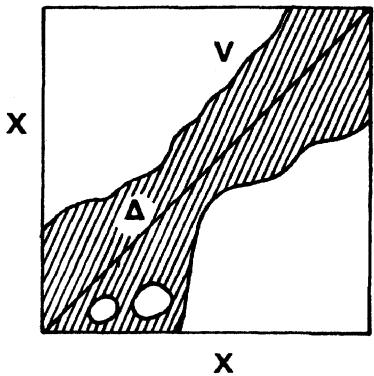
\includegraphics[keepaspectratio]{images/part001_6ce88dc6.jpg}}\\
图 2.

\(\mathfrak{U}\) 中的诸集合称为在 \(\mathbf{X}\) 上由 \(\mathfrak{U}\) 所定义的一致结构的一致邻域。赋有一致结构的集合称为一致空间。

若 V 是集合 X 上某个一致结构的一致邻域，我们可以把关系 \((x, x') \in V\) 表述为“x 与 \(x'\) 是 V-邻近的”。

注。1）为使语言更富表现力，我们可以在某些陈述中使用“x 与 y 足够接近”“x 与 y 要多接近就有多接近”这类说法。例如，我们将说，一个关系

R \(\{x,y\}\) 只要 x 与 y 足够接近便为真，如果存在一致邻域 V，使关系 \((x,y)\in V\) 蕴含 R \(\{x,y\}\)。

\begin{enumerate}
\def\labelenumi{\arabic{enumi})}
\setcounter{enumi}{1}
\tightlist
\item
  公理（U \(_{II}\)）与（U \(_{III}\)）的合取（在一致结构的其余公理之下）等价于下述公理：
\end{enumerate}

\((\mathbf{U}_a)\) 对每个 \(\mathbf{V} \in \mathfrak{U}\)，存在 \(\mathbf{W} \in \mathfrak{U}\) 使 \(\mathbf{W} \circ \overline{\mathbf{W}} \subset \mathbf{V}\) (*)。

显然 \((\mathbf{U}_{\mathrm{II}})\) 与 \((\mathbf{U}_{\mathrm{III}})\) 蕴含 \((\mathbf{U}_a)\)。反之，若 \((\mathbf{U}_a)\) 成立，我们有 \(\overline{\mathbf{W}} = \Delta \circ \overline{\mathbf{W}} \subset \mathbf{V}\)（由 \((\mathbf{U}_I)\)）；于是 \(\mathbf{W} \subset \overline{\mathbf{V}}\)，从而{[}由 \((\mathbf{F}_I)] \overline{\mathbf{V}} \in \mathfrak{U}\)。令 \(\mathbf{W}' = \mathbf{W} \cap \overline{\mathbf{W}}\)；则 \(\mathbf{W}' \in \mathfrak{U}\)（由刚才所证及公理 \((\mathbf{F}_{\mathrm{II}})\)），并且 \(\mathbf{W}' \circ \mathbf{W}' \subset \mathbf{W} \circ \overline{\mathbf{W}} \subset \mathbf{V}\)。

本章中我们始终用 \(\mathbf{V}\) 代替 \(\mathbf{V} \circ \mathbf{V}\)，一般地写 \(\mathbf{V} = \mathbf{V} \circ \mathbf{V} = \mathbf{V} \circ \mathbf{V}\)，其中 \(n > 1\) 为整数，\(\mathbf{V}\) 为 \(\mathbf{X} \times \mathbf{X}\) 的子集。

\begin{enumerate}
\def\labelenumi{\arabic{enumi})}
\setcounter{enumi}{2}
\tightlist
\item
  若 X 非空，则公理 \((U_{I})\) 蕴含 U 中没有一个集合是空集，从而 U 是 \(X \times X\) 上的一个滤子。空集上只有一个一致结构，即 \(U = \{\varnothing\}\)。
\end{enumerate}

定义 2 一致结构的一致邻域基本系是指由一致邻域组成的任一这样的族 B：每个一致邻域都含有属于 B 的一个集合。

公理 \((\mathbf{U}_{\mathbf{III}})\) 表明，若 n 为任一整数 \textgreater0 且 V 取遍某个一致邻域基本系，则诸集合 \(V^{n}\) 仍构成一个一致邻域基本系。

满足 \(V = \overline{V}^{1}\) 的一致邻域 V 称为对称的。若 V 是任一一致邻域，则 \(V \cap \overline{V}^{1}\) 与 \(V \cup \overline{V}^{1}\) 都是对称一致邻域，并且公理 \((F_{\mathrm{II}})\) 与 \((U_{\mathrm{II}})\) 表明诸对称一致邻域构成一个一致邻域基本系。

子集族 \(\mathfrak{B}\)——它由 \(\mathbf{X} \times \mathbf{X}\) 的子集组成——是 \(\mathbf{X}\) 上某个一致结构的一致邻域基本系，当且仅当 \(\mathfrak{B}\) 满足第一章 § 6 第 3 目的公理（ \(B_{\mathbf{I}}\)），并且还满足下列公理：

\((\mathbf{U}_{\mathbf{I}}^{\prime})\) \(\mathfrak{B}\) 中的每个集合都含对角线 \(\Delta\)。

\((\mathbf{U}_{\mathbf{II}}^{\prime})\) 对每个 \(\mathbf{V} \in \mathfrak{B}\)，存在 \(\mathbf{V}' \in \mathfrak{B}\) 使 \(\mathbf{V}' \subset \overline{\mathbf{V}}^1\)。

\((\mathbf{U}_{\mathbf{III}}^{\prime})\) 对每个 \(\mathbf{V} \in \mathfrak{B}\)，存在 \(\mathbf{W} \in \mathfrak{B}\) 使 \(\tilde{\mathbf{W}} \subset \mathbf{V}\)。

若 X 非空，则 X 上一致结构的一致邻域基本系是由该结构的诸一致邻域组成的滤子的一个基（第一章 § 6 第 3 目命题 3）。

(*) 我们回顾（《集合论》，R，§ 3，第 4 与第 10 目）：若 V 与 W 是 \(\mathbf{X} \times \mathbf{X}\) 的两个子集，则由对 \((x, y) \in \mathbf{X} \times \mathbf{X}\)（它们满足：\((x, z) \in \mathbf{W}\) 且 \((z, y) \in \mathbf{V}\) 对某个 \(z \in \mathbf{X}\) 成立）组成的集合记作 V o W 或 VW，而由对 \((x, y) \in \mathbf{X} \times \mathbf{X}\) 中满足 \((y, x) \in \mathbf{V}\) 者组成的集合记作 \(\overline{\mathbf{V}}\)。

一致结构的例子。* 1）在实数集 R 上可以如下定义一个称为加法一致结构的一致结构：对每个 \(\alpha > 0\)，令 \(V_{\alpha}\) 为 \(R \times R\) 中由对 \((x, y)\)（满足 \(|x - y| < \alpha\)）全体组成的子集；当 \(\alpha\) 取遍一切实数 \(> 0\) 时，诸 \(V_{\alpha}\) 构成 R 上加法一致结构的一个一致邻域基本系。类似地，在有理数集 Q 上可以定义一个一致结构（也称加法一致结构）；我们将在第三章与第四章中研究这些结构以及群上类似的一致结构。* 2）设 X 是一个集合，R 是 X 上的一个等价关系；令 C 为

R 在 \(\mathbf{X} \times \mathbf{X}\) 中的图像。于是 \(\Delta \subset \mathbf{C}\) 且 \(\tilde{\mathbf{C}} = \tilde{\mathbf{C}} = \mathbf{C}\)（《集合论》，R，§ 5，第 1 目）；因此由单独一个集合 C 组成的 \(\mathbf{X} \times \mathbf{X}\) 的子集族是 X 上某个一致结构的一致邻域基本系。特别地，若取 R 为相等关系，则 \(\mathbf{C} = \Delta\)，而相应一致结构的诸一致邻域是 \(\mathbf{X} \times \mathbf{X}\) 中含 \(\Delta\) 的一切子集；这个一致结构称为 X 上的离散一致结构，赋有这个一致结构的集合 X 称为离散一致空间。

\begin{enumerate}
\def\labelenumi{\arabic{enumi})}
\setcounter{enumi}{2}
\tightlist
\item
  在有理整数集 \(\mathbf{Z}\) 上可以如下定义一个在数论中重要的一致结构：给定一个素数 \(p\)，令 \(\mathbf{W}_n\) 为由对 \((x,y)\in \mathbf{Z}\times \mathbf{Z}\) 中满足 \(x\equiv y\)（mod \(p^n\)）者全体组成的集，这里 \(n > 0\) 为任意整数。容易验证，诸集合 \(\mathbf{W}_n\)（对固定的 \(p\)）构成 \(\mathbf{Z}\) 上某个一致结构的一致邻域基本系，该一致结构称为 \(p\) 进一致结构（参看第三章 § 6 习题 23 及以后，以及第九章 § 3 第 2 目）。
\end{enumerate}

按照一般的定义（《集合论》，R，§ 8，第 5 目），若 X 与 X' 是两个各赋有一致结构的集合，其一致邻域族分别为 U 与 U'，则 X 到 X' 上的双射 f 是 X 的一致结构到 X' 的一致结构上的同构，如果 g(U) = U'，其中 g = f × f。

例如，若 X 与 \(X'\) 是两个等势的集合，则 X 到 \(X'\) 上的每个双射都是 X 的离散一致结构到 \(X'\) 的离散一致结构上的同构。

\subsection{一致空间的拓扑}

命题 1 设 X 是赋有一致结构 U 的集合，对每个 \(x \in X\)，令 \(\mathfrak{B}(x)\) 为诸子集 \(\mathbf{V}(x)\)（\(\mathbf{X}(*)\) 的子集）组成的集，其中 V 取遍 U 的一致邻域集。则 X 上存在唯一的拓扑，使对每个 \(x \in X\)，\(\mathfrak{B}(x)\) 是 x 在该拓扑中的邻域滤子。

必须证明诸 \(\mathfrak{B}(x)\) 满足第一章 § 1 第 2 目的条件 \((\mathbf{V}_{\mathbf{I}})\)、\((\mathbf{V}_{\mathbf{II}})\)、\((\mathbf{V}_{\mathbf{III}})\) 与 \((\mathbf{V}_{\mathbf{IV}})\)。对前三个条件而言，这可由 \(\mathcal{U}\) 的诸一致邻域满足 \((\mathbf{F}_{\mathbf{I}})\)、\((\mathbf{F}_{\mathbf{II}})\) 与 \((\mathbf{U}_{\mathbf{I}})\) 立即得出。至于 \((\mathbf{V}_{\mathbf{IV}})\)，设 \(\mathbf{V}\) 是 \(\mathcal{U}\) 的一个一致邻域，\(\mathbf{W}\) 是 \(\mathcal{U}\) 的使 \(\hat{\mathbf{W}} \subset \mathbf{V}\) 的一致邻域；则当 \((x, y) \in \mathbf{W}\) 且 \((y, z) \in \mathbf{W}\) 时有 \((x, z) \in \mathbf{V}\)，从而 \(\mathbf{W}(y) \subset \mathbf{V}(x)\) 对一切 \(y \in \mathbf{W}(x)\) 成立，因此 \(\mathbf{V}(x) \in \mathfrak{B}(y)\) 对一切 \(y \in \mathbf{W}(x)\) 成立。证毕。

定义 3 命题 1 中所定义的拓扑称为一致结构 U 诱导的拓扑。

例。* 1）加法一致结构在实数集上诱导的拓扑是实直线的拓扑（第一章 § 1 第 2 目）；类似地，加法一致结构在有理数集上诱导的拓扑是有理直线的拓扑。*

\begin{enumerate}
\def\labelenumi{\arabic{enumi})}
\setcounter{enumi}{1}
\tightlist
\item
  在任何集合 X 上，离散一致结构（第 1 目例 2）诱导的拓扑都是离散拓扑。
\end{enumerate}

今后当我们谈到一致空间 X 的拓扑时，除非另有明确说明，总是指该空间的一致结构所诱导的拓扑。在集合 X 上赋以这个拓扑所得到的拓扑空间，有时称为所说一致空间的底拓扑空间。例如，当我们说一个一致空间是豪斯多夫的、或紧的、或局部紧的等等时，我们是指其底拓扑空间具有该性质。

若 X 与 \(X'\) 是两个一致空间，则 X 的一致结构到 \(X'\) 的一致结构上的任一同构 f 也是 X 到 \(X'\) 上的同胚；我们称 f 是一致空间 X 到一致空间 \(X'\) 上的同构。应当注意，X 到 \(X'\) 上的同胚未必是 X 的一致结构到 \(X'\) 的一致结构上的同构。

\pandocbounded{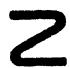
\includegraphics[keepaspectratio]{images/part001_037a61a5.jpg}}

换句话说，同一集合 X 上不同的一致结构可以诱导同一拓扑。* 例如，在 {]}0, +∞{[} 上，加法一致结构与乘法一致结构（它们是不同的：第三章 § 6 习题 17）诱导同一拓扑。*

另一个例子见 § 2 第 2 目注 1。

命题 2 设 X 是一致空间。对 X 的每个对称一致邻域 V 与 X × X 的每个子集 M，VMV 是 M 在积空间 X × X 中的邻域，且 M 在此空间中的闭包由下列公式给出

\[
\overline {{\mathbf {M}}} = \bigcap_ {\mathbf {V} \in \mathfrak {S}} \mathbf {V M V}\tag{I}
\]

其中 \(\mathfrak{S}\) 表示 \(\mathbf{X}\) 的对称一致邻域组成的集。

设 V 是 X 的一个对称一致邻域。关系 \((x, y) \in \text{VMV}\) 表示存在 M 的元素 \((p, q)\) 使 \((x, p) \in V\) 且 \((q, y) \in V\)：换句话说（因 V 对称），\(x \in V(p)\) 且 \(y \in V(q)\)，即 \((x, y) \in V(p) \times V(q)\)。由于 \(V(p) \times X(q)\) 是 \((p, q)\) 在 \(X \times X\) 中的邻域，命题的第一部分得证。关系 \((x, p) \in V\) 与 \((y, q) \in V\) 也可写成 \(p \in V(x)\)、\(q \in V(y)\) 或 \((p, q) \in V(x) \times V(y)\)。当 V 取遍 S 时，诸集合 \(V(x) \times V(y)\) 构成 \((x, y)\) 在 \(X \times X\) 中的基本邻域系；因为若 U 与 \(U'\) 是任意两个一致邻域，总存在对称一致邻域 \(V \subset U \cap U'\)，使 \(V(x) \times V(y) \subset U(x) \times U'(y)\)。因此，\(V(x) \times V(y)\) 对每个 \(V \in S\) 都与 M 相交，当且仅当 \((x, y) \in \overline{\mathbf{M}}\)，由此即得公式 (1)。

推论 1 若 A 是 X 的任一子集，V 是 X 的任一对称一致邻域，则 V(A) 是 A 在 X 中的邻域，且

\[
\overline {{{\mathbf {A}}}} = \bigcap_ {\mathbf {v} \in \mathfrak {S}} \mathbf {V} (\mathbf {A}) = \bigcap_ {\mathbf {v} \in \mathfrak {U}} \mathbf {V} (\mathbf {A})\tag{2}
\]

其中 \(\mathfrak{U}\) 表示 \(\mathbf{X}\) 中所有一致邻域组成的集。

若 \(\mathbf{M} = \mathbf{A} \times \mathbf{A}\)，则 \(\mathrm{VMV} = \mathrm{V}(\mathbf{A}) \times \mathrm{V}(\mathbf{A})\) 对任何 \(\mathbf{V} \in \mathfrak{S}\) 成立；因为关系“存在 \(p \in \mathbf{A}\) 使 \((x, p) \in \mathbf{V}"\)按定义等价于 \(x \in \mathbf{V}(\mathbf{A})\)。推论由第一章 § 4 第 2 目命题 5 与第 3 目命题 7 立即得出。

V(A) 称为 A 的 V-邻域。

若 V 是在 X × X 中开的一致邻域，则对每个 x ∈ X，V(x) 在 X 中开（第一章 § 4 第 2 目命题 4 的推论），因此 V(A)——它是 x 取遍 A 时诸 V(x) 的并——在 X 中开。另一方面，若 V 是 X × X 中的闭一致邻域，则对 X 的每个子集 A，V(A) 未必在 X 中闭（习题 3）。

\pandocbounded{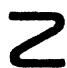
\includegraphics[keepaspectratio]{images/part001_f8cd4ad5.jpg}}

还应指出，当 V 取遍 X 的一致邻域集时，诸集合 V(A) 未必构成 A 在 X 中的基本邻域系（习题 2）。

推论 2 X 的一致邻域在 X × X 中的内部（相应地，闭包）构成 X 的一个一致邻域基本系。

若 V 是 X 的任一一致邻域，则存在对称一致邻域 W 使 \(W \subset V\)；由于 W 是 W 的邻域（命题 2），V 在 \(X \times X\) 中的内部含 W，从而是一个一致邻域。此外，由命题 2 有 \(W \subset W \subset W \subset V\)，因此 V 含某个一致邻域的闭包。

推论 3 每个一致空间都满足公理（O \(_{III}\)）。

若 \(x\) 是 \(X\) 的任一点且 \(V\) 取遍 \(X\) 的在 \(X \times X\) 中闭的一致邻域，则由推论 2，诸集合 \(V(x)\) 构成 \(x\) 在 \(X\) 中的基本邻域系，并且它们在 \(X\) 中闭（第一章 § 4 第 2 目命题 4 的推论）。

命题 3 一致空间 X 是分离的，当且仅当其一致结构的所有一致邻域之交是对角线 \(\Delta\)（即 \(X \times X\) 的对角线）。每个分离的一致空间都是正则的。

后一断言由命题 2 的推论 3 立即得出。我们已看到，闭的一致邻域构成一个一致邻域基本系（命题 2 推论 2）；若其交是 \(\Delta\)，则 \(\Delta\) 在 \(X \times X\) 中闭，从而 \(X\) 是分离的（第一章 § 8 第 1 目命题 1）。反之，若 \(X\) 分离，则对每个点 \((x, y) \notin \Delta\)，存在 \(V\)（\(X\) 的一致邻域）使 \(y \notin V(x)\)，或等价地 \((x, y) \notin V\)；于是 \(\Delta\) 是所有一致邻域之交。

若一致空间 X 分离，我们就说 X 的一致结构是分离的。若 B 是该结构的一个一致邻域基本系，则 X 分离当且仅当 B 中所有集合之交是 \(\Delta\)。

\section{一致连续函数}

\subsection{一致连续函数}

定义 1 设 \(f\) 是一致空间 \(\mathbf{X}\) 到一致空间 \(\mathbf{X}'\) 的映射；如果对每个 \(\mathbf{V}'\)（\(\mathbf{X}'\) 的一致邻域），存在 \(\mathbf{V}\)（\(\mathbf{X}\) 的一致邻域），使关系 \((x,y)\in \mathbf{V}\) 蕴含 \((f(x),f(y))\in \mathbf{V}'\)，则称 f 为一致连续的。

用更形象的说法：\(f\) 一致连续，是指 \(f(x)\) 与 \(f(y)\) 要多接近就有多接近，只要 \(x\) 与 \(y\) 足够接近。

若令 \(g = f \times f\)，则定义 1 的意思是：只要 \(V'\) 是 \(X'\) 的一致邻域，\(\overline{g}^1(V')\) 就是 \(X\) 的一致邻域。

例。1）一致空间到其自身的恒等映射是一致连续的。

\begin{enumerate}
\def\labelenumi{\arabic{enumi})}
\setcounter{enumi}{1}
\item
  一致空间到一致空间的常值映射是一致连续的。
\item
  离散一致空间到一致空间的每个映射都是一致连续的。
\end{enumerate}

命题 1 每个一致连续映射都是连续的。

这是定义的直接推论。

另一方面，一致空间 X 到一致空间 \(X'\) 的连续映射未必一致连续，* 例如 \(x \to x^{3}\)，它是 R 到自身的同胚，但关于加法一致结构不一致连续。*（见 § 4 第 1 目定理 2。）

命题 2 （a）若 \(f: \mathbf{X} \to \mathbf{X}'\) 与 \(g: \mathbf{X}' \to \mathbf{X}''\) 是两个一致连续映射，则 \(g \circ f: \mathbf{X} \to \mathbf{X}''\) 是一致连续的。

\begin{enumerate}
\def\labelenumi{(\alph{enumi})}
\setcounter{enumi}{1}
\tightlist
\item
  设 \(f\) 是一致空间 \(\mathbf{X}\) 到一致空间 \(\mathbf{X}'\) 上的双射；它是同构，当且仅当 \(f\) 与 \(f\) 的逆映射都一致连续。
\end{enumerate}

这由定义 1 借助积映射 \(f \times f\) 的解释立即得出。

\subsection{一致结构的比较}

第 1 目的命题 2 表明，我们可以取一致连续映射作为一致结构的态射（《集合论》，第四章，§ 2，第 1 目）；今后我们总假定态射就是这样选取的。按照一般的定义（《集合论》，第四章，§ 2，第 2 目），这使我们可以对给定集合 X 上的一切一致结构组成的集定义一个序关系：

定义 2 若 \(\mathfrak{U}_1\) 与 \(\mathfrak{U}_2\) 是同一集合 \(\mathbf{X}\) 上的两个一致结构，则称 \(\mathfrak{U}_1\) 比 \(\mathfrak{U}_2\) 细（而 \(\mathfrak{U}_2\) 比 \(\mathfrak{U}_1\) 粗），如果记 \(\mathbf{X}_i\) 为集合 \(\mathbf{X}\) 赋以一致结构 \(\mathfrak{U}_i\) 后所得的空间（ \(i = 1,2\)），恒等映射 \(\mathbf{X}_1 \to \mathbf{X}_2\) 一致连续。

若 \(\mathfrak{U}_1\) 比 \(\mathfrak{U}_2\) 细且异于 \(\mathfrak{U}_2\)，则称 \(\mathfrak{U}_1\) 严格地细于 \(\mathfrak{U}_2\)（而 \(\mathfrak{U}_2\) 严格地粗于 \(\mathfrak{U}_1\)）。

两个一致结构称为可比较的，如果其中一个比另一个细。

例。在集合 X 上一切一致结构组成的有序集中，离散一致结构是最细的，而最粗的一致结构是其一致邻域集由单个元素 \(X \times X\) 组成的那一个。

下述命题是第 1 目定义 1 的直接推论：

命题 3 若 \(\mathfrak{U}_1\) 与 \(\mathfrak{U}_2\) 是集合 \(X\) 上的两个一致结构，则 \(\mathfrak{U}_1\) 比 \(\mathfrak{U}_2\) 细，当且仅当 \(\mathfrak{U}_2\) 的每个一致邻域都是 \(\mathfrak{U}_1\) 的一致邻域。

推论 设 \(\mathfrak{U}_1\) 与 \(\mathfrak{U}_2\) 是集合 \(X\) 上的两个一致结构，且设 \(\mathfrak{U}_1\) 比 \(\mathfrak{U}_2\) 细；则 \(\mathfrak{U}_1\) 诱导的拓扑比 \(\mathfrak{U}_2\) 诱导的拓扑细。

这由拓扑按邻域的比较（第一章 § 2 第 2 目命题 3）立即得出。

注。1）可能发生这样的情形：一致结构 \(\mathcal{U}_1\) 严格地细于一致结构 \(\mathcal{U}_2\)，但二者诱导的拓扑相同。下面的例子表明这一点：

设 \(\mathbf{X}\) 是非空集合。对每个有限分拆 \(\varpi = (\mathrm{A}_i)_{1\leqslant i\leqslant n}\)（\(\mathbf{X}\) 的），令 \(\mathrm{V}_{\overline{\omega}}\) 表示

\[
\bigcup_ {i} \mathrm{A} _ {i} \times \mathrm{A} _ {i}.
\]

于是诸集合 \(V_{\overline{w}}\) 构成某个一致结构 \(\mathcal{U}\)（\(X\) 上的）的一致邻域基本系。因为若 \(\varpi\) 是 \(X\) 的任一有限分拆，我们有 \(\Delta \subset V_{\overline{w}}\) 且 \(V_{\overline{w}} \circ V_{\overline{g}} = \overline{V}_{\overline{w}}^{1} = V_{\overline{w}}\)（§ 1 第 1 目例 2）；又若 \(\varpi' = (B_j)\) 与 \(\varpi'' = (C_k)\) 是 \(X\) 的两个有限分拆，则诸集合 \(B_j \cap C_k\) 中非空者构成一个有限分拆 \(\varpi\)（\(X\) 的），并且 \(V_{\overline{w}} \subset V_{\overline{w}'} \cap V_{\overline{w}''}\)。称 \(\mathcal{U}\) 为 \(X\) 上有限分拆的一致结构。由 \(\mathcal{U}\) 诱导的拓扑是离散拓扑，因为对每个 \(x \in X\)，集合 \(\{x\}\) 与 \(C\{x\}\) 构成 \(X\) 的一个有限分拆。然而，若 \(X\) 无限，则显然 \(\mathcal{U}\) 严格地粗于离散一致结构。2）若 \(f: X \to X'\) 是一致连续映射，则 \(f\) 在把 \(X\) 的一致结构换成较细的一致结构、把 \(X'\) 的一致结构换成较粗的一致结构之后仍一致连续（第 1 目命题 2）。换句话说，\(X\) 的一致结构越细且 \(X'\) 的一致结构越粗，\(X\) 到 \(X'\) 的一致连续映射就越多。

\subsection{初始一致结构}

命题 4 设 X 是一个集合，\((\mathrm{Y}_{t})_{t\in I}\) 是一族一致空间，且对每个 \(t\in I\)，\(f_{t}\) 是 X 到 \(Y_{t}\) 的映射。对每个 \(t\in I\)，令 \(g_{t}\) 表示 \(f_{t}\times f_{t}\)。设 S 为 \(X\times X\) 中形如 \(\overline{g}_{t}(V_{t})\) 的子集组成的集，其中 \(t\in I\) 而 \(V_{t}\) 是 \(Y_{t}\) 的一致邻域；又设 B 为一切有限交

\[
\mathbf {U} \left(\mathrm{V} _ {\iota_ {1}}, \dots , \mathrm{V} _ {\iota_ {n}}\right) = _ {i} ^ {- 1} g _ {i} \left(\mathrm{V} _ {\iota_ {1}}\right) \cap \dots \cap^ {- 1} g _ {\iota_ {n}} \left(\mathrm{V} _ {\iota_ {n}}\right)\tag{1}
\]

组成的集，其中每个成员由 \(\mathfrak{S}\) 中的集合构成。于是 \(\mathfrak{B}\) 是某个一致结构 \(\mathfrak{U}\)（\(\mathbf{X}\) 上的）的一致邻域基本系，该一致结构是 \(\mathbf{X}\) 关于族 \((f_{\mathfrak{i}})\) 的初始一致结构（《集合论》，第四章，§ 2，第 3 目），特别地，\(\mathfrak{U}\) 是 \(\mathbf{X}\) 上使所有映射 \(f_{\mathfrak{i}}\) 都一致连续的最粗一致结构。进而言之，设 \(h\) 是一致空间 \(\mathbf{Z}\) 到 \(\mathbf{X}\) 的映射；则 \(h\) 一致连续（当 \(\mathbf{X}\) 赋有一致结构 \(\mathfrak{U}\) 时），当且仅当每个映射 \(f_{\mathfrak{i}} \circ h\) 都一致连续。

立即可以看出 \(\mathfrak{B}\) 满足公理 \((\mathbf{B}_1)\mathbf{Y}\) 与 \((\mathbf{U}_1')\)。若 \(\mathbf{W}_t = \overline{g}_t^1 (\mathbf{V}_t)\)，则 \(\overline{\mathbf{W}}_t = \overline{g}_t^1 (\overline{\mathbf{V}}_t^1)\) 且 \(\dot{\mathbf{W}}_t = \overline{g}_t^1 (\overline{\mathbf{V}}_t^2)\)；于是 \(\mathfrak{B}\) 也满足公理 \((\mathbf{U}_{\mathrm{II}}^t)\) 与 \((\mathbf{U}_{\mathrm{III}}^t)\)，从而是某个一致结构 \(\mathcal{U}\)（\(\mathbf{X}\) 上的）的一致邻域基本系。此外，由 \(\mathcal{U}\) 的定义以及第 1 目的定义 1 立即可知，\(f_{t}\) 对每个指标 \(i\in I\) 一致连续；因此（第 1 目命题 2）\(f_{t}\circ h\) 对每个 \(i\in I\) 都一致连续，只要 \(h\) 一致连续。反之，设 \(f_{t}\circ h\) 对每个 \(i\in I\) 都一致连续，并考虑一个集合 \(\mathrm{U}(\mathrm{V}_{i_t},\dots,\mathrm{V}_{i_n})\)；由假设，对每个 \(k\)（\(1\leqslant k\leqslant n\)），存在 \(\mathbf{W}_k\)（\(\mathbf{Z}\) 的一致邻域），使关系 \((z,z^{\prime})\in \mathbf{W}_k\) 蕴含 \([f_{i_k}(h(z)),f_{i_k}(h(z')))]\in \mathbf{V}_k\)；若

\[
\mathbf {W} = \bigcap_ {k} \mathbf {W} _ {k},
\]

则这 \(n\) 个关系只要 \(z\) 与 \(z'\) 是 W-邻近的便同时满足，从而有 \((h(z), h(z')) \in \mathrm{U}(\mathrm{V}_{\iota_1}, \ldots, \mathrm{V}_{\iota_n})\)，证明完成。

推论 使诸 \(f_{i}\) 一致连续的最粗一致结构 U 在 X 上诱导的拓扑，也是使诸 \(f_{i}\) 连续的最粗拓扑。

这是后一拓扑中一点的邻域定义（第一章 § 2 第 3 目命题 4）的直接推论。

初始结构的一般性质（《集合论》，第四章，§ 2，第 3 目，判别准则 CST 10）特别蕴含下列传递性质：

命题 5 设 X 是一个集合，\((Z_{\iota})_{\iota \in I}\) 是一族一致空间，\((J_{\lambda})_{\lambda \in L}\) 是 I 的一个分拆，\((Y_{\lambda})_{\lambda \in L}\) 是以 L 为指标集的一族集合。对每个 \(\lambda \in L\)，设 \(h_{\lambda}\) 是 X 到 \(Y_{\lambda}\) 的映射；对每个 \(\lambda \in L\) 与每个 \(\iota \in J_{\lambda}\)，设 \(g_{\iota \lambda}\) 是 \(Y_{\lambda}\) 到 \(Z_{\iota}\) 的映射；并令 \(f_{\iota} = g_{\iota \lambda} \circ h_{\lambda}\)。设每个 \(Y_{\lambda}\) 赋有使诸映射 \(g_{\iota \lambda} (\iota \in J_{\lambda})\) 一致连续的最粗一致结构。则使诸 \(f_{\iota}\) 一致连续的 X 上最粗的一致结构，与使诸 \(h_{\lambda}\) 一致连续的 X 上最粗的一致结构是同一个。

\subsection{一致结构的逆像；一致子空间}

设 X 是一个集合，Y 是一致空间，f 是 X 到 Y 的映射。X 上使 f 一致连续的最粗一致结构 U 称为 Y 的一致结构在 f 下的逆像。由第 3 目的命题 4 以及给出交的逆像的公式可知，Y 的一致邻域在 \(g = f \times f\) 下的诸逆像构成 U 的一致邻域基本系。由 U 诱导的拓扑是 Y 的拓扑在 f 下的逆像（第 3 目命题 4 的推论）。

注 若 \(f: \mathbf{X} \to \mathbf{Y}\) 是满射，则 \(\mathbf{Y}\) 的一致邻域是在 \(g\) 之下 \(\mathbf{X}\) 的一致邻域的直接像。

设 \(f\) 是一致空间 \(\mathbf{X}\) 到一致空间 \(\mathbf{X}'\) 的映射；它一致连续的充要条件是：在 \(f\) 之下 \(\mathbf{X}'\) 的一致结构的逆像粗于 \(\mathbf{X}\) 的一致结构。

设 A 是一致空间 X 的子集。X 的一致结构在 A 上诱导的一致结构是后者在典范单射 \(A \rightarrow X\) 下的逆像。由第 3 目命题 4，这等价于下述定义：

定义 3 设 A 是一致空间 X 的子集。A 上以 X 的一致邻域集在 A × A 上的迹为一致邻域集的那个一致结构，称为 X 的一致结构在 A 上诱导的一致结构。

由 A 上诱导的一致结构所诱导的拓扑，与 X 的拓扑在 A 上诱导的拓扑相同；集合 A 连同由 X 的一致结构与拓扑诱导的一致结构与拓扑，称为 X 的一致子空间。

若 A 是一致空间 X 的子集，且 \(f: X \to X'\) 是一致连续映射，则限制 \(f|A\) 是 A 到 \(X'\) 的一致连续映射。若 \(A' \subset X'\) 使得 \(f(X) \subset A'\)，则 X 到一致子空间 \(A'\)（\(X'\) 的）中的、与 f 有同一图像的那个映射仍一致连续（第 3 目命题 4）。

若 \(B \subset A \subset X\)，则 X 的一致子空间 B 与 X 的一致子空间 A 的一致子空间 B 相同（诱导一致结构的可递性；第 3 目命题 5）。

命题 6 设 A 是一致空间 X 的稠密子集。则一致子空间 A 的诸一致邻域在 X × X 中的闭包构成 X 的一致邻域基本系。

A × A 在 X × X 中稠密（第一章 § 4 第 3 目命题 7）。设 V 是 A 的一个开一致邻域；它是 A × A 与 X 的某个开一致邻域 U 的交。我们有 U ⊂ V̄（第一章 § 1 第 6 目命题 5），而这一关系与 V̄ ⊂ U 合在一起，依据 § 1 第 2 目命题 2 的推论 2，便证明了本命题。

\subsection{一致结构集的上确界}

每个族 \((\mathcal{U}_t)_{i\in I}\)（集合 \(X\) 上的一致结构族）都有上确界 \(\mathcal{U}\)，这里所指的有序集是 \(X\) 上所有一致结构组成的有序集；只需应用第 3 目命题 4，取 \(Y_t\) 为集合 \(X\) 赋以一致结构 \(\mathcal{U}_t\) 后所得的空间，并取 \(f_t\) 为恒等映射 \(X\to Y_t\)。由 \(\mathcal{U}\) 诱导的拓扑恰是由诸 \(\mathcal{U}_t\) 诱导的拓扑的上确界。

由第 3 目命题 4 还可得出：若 X 非空且 \(\mathcal{U}_{t}\) 是 \(\mathcal{U}_{t}\) 的一致邻域滤子，则 \(\mathcal{U}\) 的一致邻域滤子是诸滤子 \(\mathcal{U}_{t}\) 的上确界（第一章 § 6 第 2 目）。

例 若 \(\varpi\) 是任一有限分拆 \((\mathbf{A}_i)_{1 \leqslant i \leqslant n}\)（非空集合 \(\mathbf{X}\) 的），则集合 \(\mathbf{V}_{\overline{\omega}} = \bigcup_{i} (\mathbf{A}_i \times \mathbf{A}_i)\) 本身就构成

X 上某个一致结构 \(\mathfrak{U}_{\varpi}\) 的一致邻域基本系（§ 1 第 1 目例 2）；X 上有限分拆的一致结构（第 2 目注 1）就是诸一致结构 \(\mathfrak{U}_{\varpi}\) 的上确界。

注 X 上的一致结构族 \((\mathcal{U}_{i})\) 在 X 上所有一致结构组成的有序集中也有下确界，即由 X 上粗于每个 \(U_{i}\) 的一切一致结构组成的集的上确界（这样的一致结构存在，因为 X 上所有一致结构组成的集有最小元素）。但是（设 X 非空）这一一致结构的一致邻域滤子未必是诸 \(U_{i}\) 的一致邻域滤子的交，因为后一滤子未必满足公理 \((\mathrm{U}_{\mathrm{III}})\)（习题 4）。

\subsection{一致空间的积}

定义 4 若 \((\mathbf{X}_t)_{i\in I}\) 是一族一致空间，则该族的积一致空间是指积集合

\[
\mathbf {X} = \prod_ {i \in I} \mathbf {X} _ {i}
\]

并赋以使诸投影 \(pr_{t}: X \rightarrow X_{t}\) 都一致连续的最粗一致结构。这一一致结构称为诸 \(X_{t}\) 的一致结构的积，而一致空间 \(X_{t}\) 称为 X 的因子。

积一致结构在 X 上诱导的拓扑与诸 \(X_{i}\) 的拓扑的积相同（第 3 目命题 4 的推论）。

命题 7 设 \(f = (f_{t})\) 是一致空间 \(Y\) 到积一致空间 \(X = \prod_{i \in I} X_{i}\) 的映射。则 \(f\) 一致连续当且仅当每个 \(f_{t}\) 都一致连续。

由于 \(f_{i} = \mathrm{pr}_{i} \circ f\)，这是第 3 目命题 4 的一个特殊情形。

推论 设 \((\mathbf{X}_t)_{i \in I}, (\mathbf{Y}_t)_{i \in I}\) 是以同一集 I 为指标的两族一致空间。对每个 \(i \in I\)，设 \(f_t\) 是 \(\mathbf{X}_t\) 到 \(\mathbf{Y}_t\) 的映射。若每个 \(f_t\) 都一致连续，则积映射

\[
f: (x _ {i}) \rightarrow (f _ {i} (x _ {i})).
\]

反之，若诸 \(X_{i}\) 非空且 f 一致连续，则每个 \(f_{i}\) 都一致连续。

\(f\) 可写成 \(x \to (f_{i}(\mathrm{pr}_{i}x))\)，因此推论的第一部分由命题 7 得出。第二部分的证明：考虑一点 \(a = (a_{i})\)（属于 \(\prod_{i \in I} X_{i}\)），并重复第一章 § 4 第 1 目命题 1 推论 1 的论证，把其中“在 \(a\)（相应地，\(a_{x}\)）连续”一语换成“一致连续”。

初始一致结构的可递性的一般判据（第 3 目命题 5）表明，如同拓扑空间的积的情形一样（第一章 § 4 第 1 目），一致空间的积是可结合的，并且下述结论成立：

命题 8 设 X 是一个集合，\((\mathbf{Y}_t)_{t \in I}\) 是一族一致空间，且对每个 \(t \in I\)，\(f_t\) 是 X 到 \(\mathbf{Y}_t\) 的映射。设 \(f\) 是映射 \(x \to (f_t(x))\)（从 X 到 \(\mathbf{Y} = \prod_{t \in I} \mathbf{Y}_t\)），并设 \(\mathfrak{U}\) 是 X 上使诸 \(f_t\) 一致连续的最粗一致结构。则 \(\mathfrak{U}\) 是在 \(f\) 之下，Y 的积一致结构在 \(f(\mathbf{X})\) 上诱导的一致结构的逆像。

推论 对每个 \(i \in I\)，设 \(A_{i}\) 是 \(Y_{i}\) 的子空间。则在 \(A = \prod_{i \in I} A_{i}\) 上由 \(\prod_{i \in I} Y_{i}\) 的积一致结构所诱导的一致结构，与诸子空间 \(A_{i}\) 的一致结构的积相同。

此外，立即可以看出，若 \(X_{1}, X_{2}\) 是两个一致空间而 \(a_{1}\) 是 \(X_{1}\) 的任意一点，则映射 \(x_{2} \to (a_{1}, x_{2})\) 是 \(X_{2}\) 到子空间 \(\{a_{1}\} \times X_{2}\)（\(X_{1} \times X_{2}\) 的）上的同构；因此：

命题 9 设 \(f\) 是积一致空间 \(\mathbf{X}_1 \times \mathbf{X}_2\) 到一致空间 \(\mathbf{Y}\) 的一致连续映射；则每个偏映射

\[
x _ {2} \rightarrow f (x _ {1}, x _ {2})
\]

（作为 \(X_{2}\) 到 Y 的映射）都是一致连续的。

换言之，两个变元的一致连续函数对每个变元分别是一致连续的。

* 第一章 § 4 第 2 目注 2 中给出的例子表明，本命题的逆命题不成立。 *

\subsection{一致空间的逆极限}

设 I 是一个偏序集，其偏序记作 \(\alpha \leqslant \beta\)。对每个 \(\alpha \in I\)，设 \(X_{\alpha}\) 是一致空间；又对每对指标 \(\alpha, \beta\)（满足 \(\alpha \leqslant \beta\)），设 \(f_{\alpha \beta}\) 是 \(X_{\beta}\) 到 \(X_{\alpha}\) 的映射。

我们称 \((\mathbf{X}_{\alpha}, f_{\alpha\beta})\) 是一致空间的逆系统，如果 (i) \((\mathbf{X}_{\alpha}, f_{\alpha\beta})\) 是集合的逆系统（参见第一章附录第 1 目），且 (ii) 只要 \(\alpha \leqslant \beta\)，\(f_{\alpha\beta}\) 就是一致连续的。在 \(X = \varprojlim X_{\alpha}\) 上，使诸典范映射 \(f_{\alpha}: X \to X_{\alpha}\) 都一致连续的最粗一致结构，称为（关于 \(f_{\alpha\beta}\) 的）诸 \(X_{\alpha}\) 的一致结构的逆极限；赋有这一最粗一致结构的集合 X 称为一致空间的逆系统 \((\mathbf{X}_{\alpha}, f_{\alpha\beta})\) 的逆极限。第一章 § 4 第 4 目中建立的拓扑空间逆极限的所有性质（命题 9 除外）在把“拓扑”换成“一致结构”、“连续映射”换成“一致连续映射”之后仍然成立。此外：

命题 10 设 I 是有向集，\((\mathbf{X}_{\alpha}, f_{\alpha \beta})\) 是以 I 为指标的一致空间逆系统，J 是 I 的共尾子集。对每个 \(\alpha \in I\)，设 \(f_{\alpha}\) 是 \(\mathbf{X} = \varprojlim \mathbf{X}_{\alpha}\) 到 \(\mathbf{X}_{\alpha}\) 的典范映射，并用 \(g_{\alpha}\) 表示 \(f_{\alpha} \times f_{\alpha}\)。则集合族 \(\overline{g}_{\alpha}^{1}(\mathrm{V}_{\alpha})\)（其中 \(\alpha\) 取遍 J，且对每个 \(\alpha \in J\)，\(\mathrm{V}_{\alpha}\) 取遍 \(\mathrm{X}_{\alpha}\) 的一个一致邻域基本系）构成 X 的一致邻域基本系。

证明留给读者；它只需把第一章 § 4 第 4 目命题 9 的证明直接加以改编。

最后，在 \(X = \varprojlim X_{\alpha}\) 上由诸 \(X_{\alpha}\) 的一致结构的逆极限所诱导的拓扑，就是诸 \(X_{\alpha}\) 的拓扑的逆极限。

\section{完备空间}

\subsection{Cauchy 滤子}

一旦集合 X 赋有了一致结构，我们就可以定义（相对于该结构的）X 的“小”子集指的是什么：X 的“小”子集是指其中所有点彼此“非常接近”的那种子集。精确地说：

定义 1 若 X 是一致空间而 V 是 X 的一致邻域，则称 X 的子集 A 是 V-小集，如果 A 的任意两点都 V-邻近（换言之，A × A ⊂ V）。

命题 1 在一致空间 X 中，若两个集合 A 与 B 都是 V-小集且相交，则其并 A ∪ B 是 V-小集。

设 \(x\) 与 \(y\) 是 \(A \cup B\) 的任意两点，并设 \(Z \in A \cap B\)。则 \((x, z) \in V\) 且 \((z, y) \in V\)，从而 \((x, y) \in \mathring{V}\)。

定义 2 滤子 \(\mathfrak{F}\)（一致空间 \(\mathbf{X}\) 上的）称为 Cauchy 滤子，如果对 X 的每个一致邻域 V，存在 X 的一个子集，它是 V-小集且属于 \(\mathfrak{F}\)。

这里我们同样可以借助“足够小的集合”与“要多小有多小的集合”这些说法使语言更形象；于是定义 2 可以改述为：Cauchy 滤子就是包含任意小的集合的滤子。

无穷序列 \((u_n)\)（一致空间 \(X\) 的点列）称为 Cauchy 序列，如果与该序列相伴的初等滤子是 Cauchy 滤子。这等价于说：对每个一致邻域 \(V\)（\(X\) 的），存在整数 \(n_0\)，使得对一切满足 \(m \geqslant n_0\) 与 \(n \geqslant n_0\) 的整数 m 与 n，都有 \((u_m, u_n) \in V\)。

命题 2 在一致空间 X 上，每个收敛滤子都是 Cauchy 滤子。

若 \(x\) 是 \(X\) 的任意一点，且 \(V\) 是 \(X\) 的任意对称一致邻域，则邻域 \(V(x)\)（\(x\) 的）是 \(V\)-小集。若 \(\mathfrak{F}\) 是收敛于 \(x\) 的滤子，则 \(\mathfrak{F}\) 中有一个集合含于 \(V(x)\)，因而是 \(V\)-小集。

显然，每个细于某个 Cauchy 滤子的滤子都是 Cauchy 滤子。

命题 3 设 \(f: \mathbf{X} \to \mathbf{X}'\) 是一致连续映射。则在 \(f\) 之下，\(\mathbf{X}\) 上 Cauchy 滤子基的像是 \(\mathbf{X}'\) 上的 Cauchy 滤子基。

设 \(g = f \times f\)。若 \(V'\) 是 \(X'\) 的一致邻域，则 \(\overline{g}^1(V')\) 是 \(X\) 的一致邻域，且在 \(f\) 之下，\(\overline{g}^1(V')\)-小集的像是 \(V'\)-小集；由此即得结论。

特别由此可得：若把一致空间 X 的一致结构换成较粗的一致结构，则关于原来一致结构的每个 Cauchy 滤子关于新一致结构仍是 Cauchy 滤子。

这一事实很容易按下述形式记住：一致结构越细，Cauchy 滤子就越少。

命题 4 设 X 是一个集合，\((\mathbf{Y}_i)_{i\in I}\) 是一族一致空间，且对每个 \(i\in I\)，\(f_i\) 是 X 到 \(\mathbf{Y}_i\) 的映射。设 X 赋有最粗的一致结构 \(\mathcal{U}\)，使诸 \(f_i\) 都一致连续。则 X 上的滤子基 \(\mathcal{B}\) 是 Cauchy 滤子基的充要条件是：\(f_i(\mathcal{B})\) 是 \(\mathbf{Y}_i\) 上的 Cauchy 滤子基（对每个 \(i\in I\)）。

由命题 3，条件是必要的。反之，设条件满足，并设 \(\mathbf{U}(\mathbf{V}_{\iota_1},\ldots ,\mathbf{V}_{\iota_n})\) 是一致结构 \(\mathfrak{U}\) 的一个一致邻域{[}§ 2 第 3 目公式 (1){]}。由假设，对每个指标 \(k\)，存在集合 \(\mathbf{M}_k\in \mathfrak{B}\)，使 \(f_{\iota_k}(\mathbf{M}_k)\) 是 \(\mathbf{V}_{\iota_k}\)-小集 ( \(\iota \leqslant k\leqslant n\) )。设 \(\mathbf{M}\) 是 \(\mathfrak{B}\) 中含于诸 \(\mathbf{M}_k\)（\(\iota \leqslant k\leqslant n\)）的一个集合；则对每对点 \(x,x^{\prime}\)（\(\mathbf{M}\) 的），有 \([f_{\iota_k}(x),f_{\iota_k}(x')]\in \mathbf{V}_{\iota_k}\)（\(\iota \leqslant k\leqslant n\)），从而

\[
(x, x ^ {\prime}) \in \mathrm{U} (\mathrm{V} _ {t _ {1}}, \dots , \mathrm{V} _ {t _ {n}}).
\]

证明完毕。

推论 1 若一致空间 X 上的 Cauchy 滤子在 X 的子集 A 上诱导出一个滤子，则该滤子是一致子空间 A 上的 Cauchy 滤子。

推论 2 滤子基 \(\mathfrak{B}\)（一致空间的积 \(\prod_{i\in I}X_i\) 上的）是 Cauchy 滤子基的充要条件是：对每个 \(i\in I\)，\(\operatorname{pr}_i(\mathfrak{B})\) 是 \(X_i\) 上的 Cauchy 滤子基。

\subsection{极小 Cauchy 滤子}

一致空间 X 上 Cauchy 滤子组成的集的（关于包含关系的）极小元素，称为 X 上的极小 Cauchy 滤子。

命题 5 设 X 是一致空间。对 X 上每个 Cauchy 滤子 F，存在唯一的粗于 F 的极小 Cauchy 滤子 \(\mathfrak{F}_0\)。若 B 是 F 的基，S 是 X 的对称一致邻域的一个基本系，则诸集合 V(M)（M ∈ B, V ∈ S）构成 \(\mathfrak{F}_0\) 的一个基。

若 M 与 \(M'\) 属于 B，V 与 \(V'\) 属于 S，则存在集合 \(M'' \in B\)（相应地 \(V'' \in S\)），使 \(M'' \subset M \cap M'\)（相应地 \(V'' \subset V \cap V'\)）；于是 \(V''(M'') \subset V(M) \cap V'(M')\)，因而诸集合 \(V(M)\)（ \(M \in B\)，\(V \in S\) ）确实构成 X 上一个滤子 \(F_0\) 的基。进而，若 M 是 V-小集，

则 V(M) 是 V-小集；因此 \(\mathfrak{F}_0\) 是 Cauchy 滤子，且显然粗于 \(\mathfrak{F}\)。为完成证明，只需证明：若 \(\mathfrak{G}\) 是粗于 \(\mathfrak{F}\) 的 Cauchy 滤子，则 \(\mathfrak{G}\) 细于 \(\mathfrak{F}_0\)。对每个 M ∈ \(\mathfrak{B}\) 与每个 V ∈ \(\mathfrak{S}\)，存在一个 V-小集 N ∈ \(\mathfrak{G}\)；由于 N ∈ \(\mathfrak{F}\)，N 与 M 相交；于是 N ⊂ V(M)，从而 V(M) ∈ \(\mathfrak{G}\)。

推论 1 对每个 \(x \in \mathbf{X}\)，邻域滤子 \(\mathfrak{B}(x)\)（\(x\) 在 \(\mathbf{X}\) 中的）是极小 Cauchy 滤子。

在命题 5 中取 \(\mathfrak{F}\) 为 \(\mathbf{X}\) 中含 \(x\) 的一切子集组成的滤子，并取 \(\mathfrak{B}\) 由单个元素 \(\{x\}\) 组成。

推论 2 Cauchy 滤子 F 的每个聚点 x 都是 F 的极限点。

存在一个滤子 \(\mathfrak{G}\)，它既细于 \(\mathfrak{F}\) 又细于 \(\mathfrak{B}(x)\)（第一章 § 7 第 2 目命题 4）；由于 \(\mathfrak{F}\) 是 Cauchy 滤子，\(\mathfrak{G}\) 也是。若 \(\mathfrak{F}_0\) 是粗于 \(\mathfrak{F}\) 的唯一的极小 Cauchy 滤子，则 \(\mathfrak{F}_0\) 与 \(\mathfrak{B}(x)\) 都是粗于 \(\mathfrak{G}\) 的极小 Cauchy 滤子。因此 \(\mathfrak{F}_0 = \mathfrak{B}(x)\)，这表明 \(\mathfrak{F}\) 收敛于 \(x\)。

推论 3 凡粗于某个收敛于点 x 的滤子的 Cauchy 滤子，也收敛于 x。

这是推论 2 的一个推论。

推论 4 若 \(\mathfrak{F}\) 是极小 Cauchy 滤子，则 \(\mathfrak{F}\) 的每个集合都有非空的内部，且该内部也属于 \(\mathfrak{F}\)（换言之，\(\mathfrak{F}\) 具有一个由开集组成的基）。

设 V 是 X 的任一一致邻域；则存在开的一致邻域 \(U \subset V\)（§ 1 第 2 目命题 2 的推论 2）。对 X 的每个子集 M，\(U(M)\) 是开集且含于 \(V(M)\)；于是由命题 5 即得结论。

\subsection{完备空间}

在一致空间 X 中，Cauchy 滤子未必有极限点。

例。1）考虑序列 \((u_{n})\)（在有理直线 \(\mathbf{Q}\) 上），它由下式定义：

\[
\text { by } \quad u _ {n} = \sum_ {p = 0} 2 ^ {- p (p + 1) / 2}. \quad \text { If } \quad m > n \quad \text { we   have }\tag{1}
\]

\[
\left| u _ {m} - u _ {n} \right| \leqslant 2 ^ {- n (n + 3) / 2}
\]

因而 \((u_{n})\) 是 Cauchy 序列。但这一序列在 \(\mathbf{Q}\) 中没有极限；因为若有理数 \(a / b\) 是 \((u_{n})\) 的极限，则由 (1)，对所有 \(n\) 我们应有

\[
\left| a / b - h _ {n} / 2 ^ {n (n + 1) / 2} \right| \leqslant 1 / 2 ^ {n (n + 3) / 2}
\]

其中 \(h_n\) 是（依赖于 \(n\) 的）整数；即

\[
\left| a. 2 ^ {n (n + 1) / 2} - b h _ {n} \right| \leqslant b. 2 ^ {- n}
\]

对所有 n 成立。现在，对一切 n，这一不等式的左端都是整数，因而只要 n 大于某个整数 \(n_{0}\)（满足 \(b < 2^{n_{0}}\)），它就必须为零；于是应有 \(a/b = u_{n}\)（对所有 \(n > n_{0}\)），这是荒谬的。

\begin{enumerate}
\def\labelenumi{\arabic{enumi})}
\setcounter{enumi}{1}
\tightlist
\item
  设 X 是无穷集合，并考虑 X 上有限分拆的一致结构（§ 2 第 2 目注 1）。X 上的每个超滤子 F 都是
\end{enumerate}

关于这一一致结构的 Cauchy 滤子。因为若 \((\mathbf{A}_{i})\) 是 X 的一个有限分拆，且

\[
\mathbf {V} = \bigcup_ {i} (\mathbf {A} _ {i} \times \mathbf {A} _ {i})
\]

是其对应的一致邻域，则至少有一个 \(A_{i}\) 属于 F（第一章 § 6 第 4 目命题 5 的推论），而 \(A_{i}\) 是 V-小集。另一方面，X 是无穷离散空间，因而不是紧的，从而 X 上存在不收敛的超滤子。

定义 3 完备空间是指每个 Cauchy 滤子都收敛的一致空间。

因此，在完备空间中，每个 Cauchy 序列（第 1 目）都收敛。例 在离散一致空间 X 上，Cauchy 滤子是平凡超滤子（第一章 § 6 第 4 目），因而收敛；从而 X 是完备的。

由第 1 目的定义 2 与定义 3 以及第 1 目的命题 2，我们推出下述命题，它称为 Cauchy 判别准则：

命题 6 设 \(\mathfrak{F}\) 是集合 X 上的滤子，\(f\) 是 X 到完备一致空间 \(\mathbf{X}'\) 的映射。则 \(f\) 关于 \(\mathfrak{F}\) 有极限的充要条件是：\(\mathfrak{F}\) 在 \(f\) 下的像是 Cauchy 滤子基。

这一判别准则表明了完备空间在涉及极限概念的一切问题中的重要性：如果一个函数在完备空间中取值，我们就可以在事先不知道极限值的情况下证明极限的存在；倘若极限的定义是我们掌握的仅有的收敛判别准则，这就不可能做到。

细于完备空间的一致结构的一致结构，未必是完备空间的一致结构（习题 2）。然而，我们有下述命题：

命题 7 设 \(\mathcal{U}_1, \mathcal{U}_2\) 是集合 \(X\) 上的两个一致结构，\(\mathfrak{C}_1, \mathfrak{C}_2\) 分别是这些一致结构诱导的拓扑。假设 \(\mathcal{U}_1\) 细于 \(\mathcal{U}_2\)，且存在 \(\mathcal{U}_1\) 的一个一致邻域基本系，其中的元素作为 \(X \times X\) 的子集在拓扑 \(\mathfrak{C}_2 \times \mathfrak{C}_2\) 中是闭的。则滤子 \(\mathfrak{F}\)（\(X\) 上的）在拓扑 \(\mathfrak{C}_1\) 中收敛的充要条件是：它在一致结构 \(\mathcal{U}_1\) 中是 Cauchy 滤子，且在拓扑 \(\mathfrak{C}_2\) 中收敛。

这些条件显然是必要的，因为 \(\mathfrak{G}_2\) 粗于 \(\mathfrak{G}_1\)。反之，设条件满足，并设 \(x\) 是 \(\mathfrak{F}\) 关于 \(\mathfrak{G}_2\) 的极限点；我们将证明 \(x\) 是 \(\mathfrak{F}\) 关于 \(\mathfrak{G}_1\) 的极限。设 \(V\) 是 \(\mathfrak{U}_1\) 的一个对称一致邻域，它在拓扑 \(\mathfrak{G}_2 \times \mathfrak{G}_2\) 中是闭的。由假设，\(\mathfrak{F}\) 含有一个集合 \(M\)，它是 \(V\)-小集；于是若 \(x' \in M\)，我们就有 \(M \subset V(x')\)。但 \(V(x')\) 在拓扑 \(\mathfrak{G}_{2}\) 中是闭的；因此，\(x\) 位于 \(\mathbf{M}\) 关于 \(\mathfrak{G}_{2}\) 的闭包中，故必属于 \(\mathbf{V}(x')\)。由此得出 \(\mathbf{M} \subset \mathbf{V}(x)\)，命题得证。

推论 在命题 7 的条件下，若 \(\mathfrak{U}_2\) 是完备空间的一致结构，则 \(\mathfrak{U}_1\) 也是完备空间的一致结构。

因为此时每个关于 \(U_{1}\) 的 Cauchy 滤子都是关于 \(U_{2}\) 的 Cauchy 滤子，从而在拓扑 \(G_{2}\) 中收敛。

注意，当 \(\mathcal{C}_1 = \mathcal{C}_2\) 时（§ 1 第 2 目命题 2 的推论 2），命题 7 的推论的假设成立。

\subsection{完备空间的子空间}

命题 8 完备空间的每个闭子空间都是完备的。豪斯多夫一致空间（完备与否）的每个完备子空间都是闭的。

设 X 是完备空间，A 是 X 的闭子空间。若 F 是 A 上的 Cauchy 滤子，则它是 X 上的 Cauchy 滤子基（第 1 目命题 3），因而收敛于某点 \(x \in X\)；但由于 A 是闭的，我们有 \(x \in A\)，因此 F 在子空间 A 中收敛。

现在设 A 是豪斯多夫一致空间 X 的非闭子集，且 \(b \in \overline{\mathbf{A}} - \mathbf{A}\)。b 在 X 中的邻域滤子 B 在 A 上的迹 \(\mathfrak{B}_{\mathbf{A}}\) 是 A 上的 Cauchy 滤子；但它不能收敛于某点 \(c \in \mathbf{A}\)，否则 c 将是 B 的极限点（第 2 目命题 5 推论 3），而这是荒谬的，因为 \(b \neq c\) 且 X 是豪斯多夫的。

命题 9 设 X 是一致空间，A 是 X 的稠密子集，且 A 上每个 Cauchy 滤子基都在 X 中收敛。则 X 是完备的。

只需证明 X 上每个极小 Cauchy 滤子 \(\mathfrak{F}\) 都收敛。由于 A 稠密，且 \(\mathfrak{F}\) 的每个集合都有非空内部（第 2 目命题 5 推论 4），迹 \(\mathfrak{F}_{\mathrm{A}}\)（\(\mathfrak{F}\) 在 A 上的）是 A 上的 Cauchy 滤子，因而收敛于某点 \(x_{0} \in \mathrm{X}\)。由于 \(\mathfrak{F}\) 粗于由 \(\mathfrak{F}_{\mathrm{A}}\) 在 X 上生成的滤子，故 \(\mathfrak{F}\) 收敛于 \(x_{0}\)（第 2 目命题 5 推论 3）。

\subsection{完备空间的积与逆极限}

命题 10 完备一致空间的每个积都是完备的。反之，若非空一致空间的一个积是完备的，则每个因子都是完备一致空间。

第一个断言是积空间上 Cauchy 滤子与收敛滤子的刻画（第 1 目命题 4 推论 2，以及第一章 § 7 第 6 目命题 10 推论 1）的推论。反之，设

\[
\mathbf {X} = \prod_ {i \in I} \mathbf {X} _ {i}
\]

是完备的（诸 \(X_{t}\) 非空），并设 \(F_{x}\) 是 \(X_{x}\) 上的一个 Cauchy 滤子。对每个 \(t \neq x\)，设 \(F_{t}\) 是 \(X_{t}\) 上的一个 Cauchy 滤子，并考虑积滤子（第一章 § 6 第 7 目）

\[
\mathfrak {F} = \prod_ {i \in I} \mathfrak {F} _ {i} \text { on } X;
\]

\(\mathfrak{F}\) 是 Cauchy 滤子（第 1 目命题 4 推论 2），因而是收敛的，从而每个 \(\mathrm{pr}_{\mathbf{x}}\mathfrak{F} = \mathfrak{F}_{\mathbf{x}}\) 也收敛（第一章 § 7 第 6 目命题 10 推论 1）。

推论 设 \((\mathbf{X}_{\alpha}, f_{\alpha\beta})\) 是一致空间的逆系统。若诸 \(X_{\alpha}\) 是豪斯多夫的且完备的，则 \(X = \varprojlim X_{\alpha}\) 也是。

因为 X 是豪斯多夫的，并且可以与 \(\prod_{i\in I}X_{\alpha}\) 的一个闭子空间恒同

（第一章 § 8 第 2 目命题 7 推论 2）；于是该推论由命题 10 与命题 8（第 4 目）得出。

完备豪斯多夫一致空间 \(X_{\alpha}\) 的逆极限可以是空的，即使所有 \(X_{\alpha}\) 都非空且所有 \(f_{\alpha\beta}\) 都是满射，离散空间的情形即表明这一点（《集合论》，第三章，§ 1，习题 32）。然而，我们有下述定理：

定理 1（Mittag-Leffler） 设 \((\mathbf{X}_{\alpha}, f_{\alpha\beta})\) 是完备豪斯多夫一致空间的逆系统，其指标集 I 是具有可数共尾子集的有向集；再设对每个 \(\alpha \in I\)，\(X_{\alpha}\) 具有可数的一致邻域基本系 (*)。最后，设对每个 \(\alpha \in I\)，存在满足下述条件的指标 \(\beta \geqslant \alpha\)：

\((\mathbf{ML}_{\alpha \beta})\) 对每个 \(\gamma \geqslant \beta, f_{\alpha \gamma}(\mathbf{X}_{\gamma})\) 在 \(f_{\alpha \beta}(\mathbf{X}_{\beta})\) 中稠密。

设 \(\mathbf{X} = \varprojlim \mathbf{X}_{\alpha}\)，并设 \(f_{\alpha}\) 是典范映射 \(\mathbf{X} \to \mathbf{X}_{\alpha}\)。则对每个 \(\alpha \in \overleftarrow{\mathbf{I}}\) 与每个 \(\beta \geqslant \alpha\)（满足 \((\mathbf{ML}_{\alpha\beta})\)），\(f_{\alpha}(\mathbf{X})\) 在 \(f_{\alpha\beta}(\mathbf{X}_{\beta})\) 中稠密（因而 \(\mathbf{X}\) 非空，只要诸 \(\mathbf{X}_{\alpha}\) 均非空）。

设 \((\lambda_{n})\) 是 I 中共尾的指标序列。从指标 \(\alpha_0 \in \mathbf{I}\) 出发，递归地定义递增序列 \((\alpha_{n})\)，使 \(\alpha_{n} \geqslant \lambda_{n}\) 且 \((\mathrm{ML}_{\alpha_{n}, \alpha_{n+1}})\) 为真。显然序列 \((\alpha_{n})\) 在 I 中共尾。我们将用 \(f_{mn}\) 代替 \(f_{\alpha_m\alpha_n}\)（当 \(m \leqslant n\) 时），并令 \(f_{n,n+1}(\mathbf{X}_{\alpha_{n+1}}) = \mathbf{Y}_n\)。于是，若 \(m \leqslant n\)，则 \(f_{mn}(\mathbf{Y}_n)\) 在 \(\mathbf{Y}_m\) 中稠密；因为按定义，\(f_{m,n+1}(\mathbf{X}_{\alpha_{n+1}})\) 在

\[
f _ {m, m + 1} \left(\mathrm{X} _ {\alpha_ {m + 1}}\right) = \mathrm{Y} _ {m}, \quad \text { and } \quad f _ {m, n + 1} \left(\mathrm{X} _ {\alpha_ {n + 1}}\right) = f _ {m n} \left[ f _ {n, n + 1} \left(\mathrm{X} _ {\alpha_ {n + 1}}\right) \right] = f _ {m n} \left(\mathrm{Y} _ {n}\right).
\]

对 \(n\) 与 \(k\) 用归纳法，可以定义闭对称一致邻域的基本系 \((\mathbf{V}_{kn})_{k\in \mathbb{N}}\)（\(\mathbf{X}_{\alpha_n}\) 的，对每个 \(n\)），使得

\begin{enumerate}
\def\labelenumi{(\arabic{enumi})}
\setcounter{enumi}{1}
\tightlist
\item
\end{enumerate}

\[
\begin{array}{c} \mathbf {V} _ {k + 1, n} ^ {2} \subset \mathbf {V} _ {k n}, \\ (f _ {n, n + 1} \times f _ {n, n + 1}) (\mathbf {V} _ {k, n + 1}) \subset \mathbf {V} _ {k n}. \end{array}\tag{3}
\]

实际上，设 \((\mathbf{U}_{kn})_{k\in\mathbb{N}}\) 是 \(X_{\alpha_{n}}\) 的一个一致邻域基本系。若假设对给定的 n，\(V_{kn}\) 已对所有 \(k\in N\) 定义，则由于 \(f_{n,n+1}\) 一致连续，我们可以对 k 用归纳法定义一致邻域 \(V_{k,n+1}\)，使 (3) 成立且

\[
\mathbf {\dot {V}} _ {k + 1, n + 1} ^ {2} \subset \mathbf {V} _ {k, n + 1} \cap \mathbf {U} _ {k + 1, n + 1}
\]

断言得证。

现在设 \(x_0 \in Y_0\)。我们将证明，对每个整数 \(k > 0\)，存在一点 \(z \in X\)，使 \([x_0, f_{\alpha_0}(z)] \in V_{k-1,0}\)；这就证明了定理。由于 \(f_{n,n+1}(Y_{n+1})\) 在 \(Y_n\) 中稠密，我们可以归纳地定义点列 \(x_n \in Y_n\)，使得

\[
\left[ x _ {n}, f _ {n, n + 1} \left(x _ {n + 1}\right) \right] \in \mathrm{V} _ {k + n, n}.\tag{4}
\]

由 (3) 推出，若 \(m \leqslant n\)，则

\[
\left[ f _ {m n} (x _ {n}), f _ {m, n + 1} (x _ {n + 1}) \right] \in \mathbf {V} _ {k + n, m}.\tag{5}
\]

由此我们断定，对固定的 \(m\)，序列 \((f_{mn}(x_n))_{n\geqslant m}\) 是 \(\mathbf{X}_{\alpha_m}\) 中的 Cauchy 序列，从而收敛于一点 \(z_m\)；因为由 (5) 用归纳法可得，对每对整数 \(p\geqslant m,q > 0\)，我们有

\[
\left[ f _ {m p} (x _ {p}), f _ {m, p + q} (x _ {p + q}) \right] \in \mathrm{V} _ {k + p + q - 1, m} \circ \mathrm{V} _ {k + p + q - 2, m} \circ \dots \circ \mathrm{V} _ {k + p, m}\tag{6}
\]

而由 (2) 显然 (6) 的右端含于 \(V_{k+p-1,m}\)。令 q 无限增大；我们特别推出，当 m=p=0 时有 \((x_{0},z_{0})\in\mathbf{V}_{k-1,0}\)，因为 \(V_{k-1,0}\) 是闭的。另一方面，由关系 \(z_{m}=\lim_{n\to\infty}f_{mn}(x_{n})\) 以及 \(f_{m,m+1}\) 的连续性，我们推出 \(f_{m,m+1}(z_{m+1})=z_{m}\)（对每个 \(m\geqslant0\)）。对每个 \(\gamma\in I\)，至少存在一个整数 n 使 \(\alpha_{n}\geqslant\gamma\)；令 \(z_{\gamma} = f_{\gamma, \alpha_n}(z_n)\)，我们立即验证：\(z_{\gamma}\) 不依赖于 \(n\) 的取值（其中 \(\alpha_n \geqslant \gamma\)），且如此定义的族 \((z_\alpha)_{\alpha \in \mathbf{I}}\) 是 \(z\)（\(\mathbf{X} = \varprojlim \mathbf{X}_\alpha\) 的一个点）。由于 \(f_{\alpha_0}(z) = z_0\)，证明完毕。

推论 1 设 \((\mathbf{X}_{\alpha}, f_{\alpha\beta})\) 是以具有可数共尾子集的有向集 I 为指标集的集合逆系统，并设诸 \(f_{\alpha\beta}\) 都是满射。则若 \(X = \varprojlim X_{\alpha}\)，典范映射 \(f_{\alpha}: X \to X_{\alpha}\) 对每个 \(\alpha \in I\) 都是满射。

给每个 \(X_{\alpha}\) 赋以离散一致结构，并应用定理 1。

推论 2 设 I 是具有可数共尾子集的有向集。设 \((\mathbf{X}_{\alpha}, f_{\alpha \beta})\) 与 \((\mathbf{X}_{\alpha}^{\prime}, f_{\alpha \beta}^{\prime})\) 是以 I 为指标集的两个集合逆系统，且对每个 \(\alpha \in I\)，设 \(u_{\alpha}: \mathbf{X}_{\alpha} \to \mathbf{X}_{\alpha}^{\prime}\) 是一个映射，使得诸 \(u_{\alpha}\) 构成映射的逆系统。令 \(u = \varprojlim u_{\alpha}\)。设 \(x = (x_{\alpha}^{\prime})\) 是

\[
\mathrm{X} ^ {\prime} = \varprojlim \mathrm{X} _ {\alpha} ^ {\prime}
\]

的一个元素，它满足下述条件：对每个 \(\alpha \in I\)，存在指标 \(\beta \geqslant \alpha\)，使得对所有 \(\gamma \geqslant \beta\) 有 \(f_{\alpha \gamma}(\overline{u}_{\gamma}^{1}(x_{\gamma})) = f_{\alpha \beta}(\overline{u}_{\beta}^{1}(x_{\beta}^{\prime}))\)。则存在元素 \(x \in X\)，使 \(u(x) = x'\)。

对集合逆系统 \(\overline{u}_{\alpha}^{1}(x_{\alpha}^{\prime})\)（其中每个集合都赋以离散一致结构）应用定理 1。

* 例 设在 C 中给定：(i) 互异点组成的序列 \((a_{n})\)，使序列 \((|a_{n}|)\) 递增且趋于 \(+\infty\)；(ii) 对每个 \(n\)，一个有理函数 \(z \to \mathbb{R}_{n}(z)\)，它定义在 \(\mathbf{C} - \{a_{n}\}\) 中且在 \(a_{n}\) 处有极点；(iii) 以 0 为中心的递增开圆盘序列 \((\mathbf{B}_{n})\)，其并为 \(\mathbf{C}\)，且没有任何 \(a_{k}\) 位于诸圆盘 \(\mathbf{B}_{n}\) 中任何一个的边界上。对每个 \(n\)，令 \(\mathbf{B}_{n}^{\prime}\) 表示 \(\overline{\mathbf{B}}_{n}\) 与 \(\mathbf{C}\) 中由点 \(a_{n}\) 组成的集合的余集之交；并令 \(\mathbf{X}_{n}\) 表示所有映射

\[
z \rightarrow \mathrm{S} (z) = \mathrm{P} (z) + \sum_ {a _ {k} \in \mathrm{B} _ {n}} \mathrm{R} _ {k} (z)
\]

（自 \(\mathbf{B}_n'\) 到 \(\mathbf{C}\)）的集合，其中 \(\mathbf{P}\) 是一个函数在 \(\mathbf{B}_n'\) 上的限制，该函数在 \(\overline{\mathbf{B}}_n\) 上连续且在 \(\mathbf{B}_n\) 内全纯。我们在 \(\mathbf{X}_n\) 中定义度量：

\[
d _ {n} \left(\mathrm{S} _ {1}, \mathrm{S} _ {2}\right) = \sup _ {z \in \mathrm{B} _ {n} ^ {\prime}} | \mathrm{S} _ {1} (z) - \mathrm{S} _ {2} (z) |.
\]

容易验证 \(\mathbf{X}_n\) 关于这个度量是完备的。最后，对 \(n \leqslant m\)，我们定义映射 \(f_{nm}: \mathbf{X}_m \to \mathbf{X}_n\)，使得若 \(\mathbf{S} \in \mathbf{X}_m\)，则 \(f_{nm}(\mathbf{S})\) 是 \(\mathbf{S}\) 在 \(\mathbf{B}_n'\) 上的限制。显然诸 \(f_{nm}\) 都一致连续，且 \((\mathbf{X}_n, f_{nm})\) 是一致空间的逆系统。于是，逆极限 \(X = \varprojlim X_{n}\) 的元素可以典范地恒同于 C 上的一个亚纯函数 F，其仅有的极点是诸点 \(a_{n}\)，并且对每个 n，\(\mathrm{F}(z) - \mathrm{R}_{n}(z)\) 在 \(a_{n}\) 处全纯。经典的 Mittag-Leffler 定理断言 X 非空；由定理 1，我们只需对所有 n 验证条件 \((\mathrm{ML}_{nn})\)。~设

\[
\mathrm{S} _ {n} = \mathrm{P} _ {n} + \sum_ {a _ {k} \in \mathrm{B} _ {n}} \mathrm{R} _ {k}
\]

是 \(\mathbf{X}_n\) 的一个元素，其中 \(\mathbf{P}_n\) 在 \(\overline{\mathbf{B}}_n\) 上连续且在 \(\mathbf{B}_n\) 内全纯；对任意 \(m \geqslant n\)，令 \(\mathbf{Q}_{mn}\) 为

\[
\sum_ {a _ {h} \in \mathrm{B} _ {m} - \mathrm{B} _ {n}} \mathrm{R} _ {h} \quad \text { to } \quad \mathrm{B} _ {n} ^ {\prime};
\]

后一和式是 \(\bar{\mathbf{B}}_n\) 的某个邻域中的全纯函数，因此（由 Taylor 定理）对每个 \(\varepsilon > 0\)，存在多项式 \(\mathbf{P}_{mn}\)，使 \(|\mathbf{Q}_{mn}(\mathbf{Z}) - \mathbf{P}_{mn}(z)| \leqslant \varepsilon\) 在 \(\mathbf{B}_n\) 中成立；若 \(\mathbf{S}_m\) 是 \(\mathbf{S}_n + \mathbf{Q}_{mn} - \mathbf{P}_{mn}\) 在 \(\mathbf{B}_m'\) 上的限制，则我们有 \(\mathbf{S}_m \in \mathbf{X}_m\)，且 \(|\mathbf{S}_m(z) - \mathbf{S}_n(z)| \leqslant \varepsilon\) 在 \(\mathbf{B}_n'\) 中成立。证明完毕。 *

\subsection{一致连续函数的延拓}

当所讨论的函数取值于完备豪斯多夫一致空间时，连续延拓定理（第一章 § 8 第 5 目定理 1）有重要的补充。

命题 11 设 A 是拓扑空间 X 的稠密子集，并设 f 是 A 到完备豪斯多夫一致空间 X' 中的一个映射。则 f 可由连续性延拓到 X，当且仅当对每个 x ∈ X，x 在 X 中的邻域滤子在 A 上的迹经 f 的像是 X' 中的 Cauchy 滤子基。

这可由连续延拓定理（出处同上）得出，因为 \(X'\) 是正则的（§ 1 第 2 目命题 3），且在 \(X'\) 上收敛滤子等同于 Cauchy 滤子。

当 X 还是一致空间时，有下述定理：

定理 2 设 \(f\) 是定义在稠密子空间 \(A\)（一致空间 \(X\) 的）上、取值于完备豪斯多夫一致空间 \(X'\) 的函数，并设 \(f\) 在 \(A\) 上一致连续。则 \(f\) 可由连续性延拓到整个 \(X\)，且延拓函数 \(\overline{f}\) 一致连续。

\(\overline{f}\) 的存在性是第 1 目命题 3 与命题 11 的直接推论。让我们证明 \(\overline{f}\) 一致连续。设 \(V'\) 是 \(X'\) 的一个闭对称一致邻域，并设 \(V\) 是 \(X\) 的一致邻域，使得当 \(x\) 与 \(y\) 属于 \(A\) 且为 \(V\) -邻近时，则 \(f(x)\) 与 \(f(y)\)

是 V' -邻近的。我们可以假设 V 是 A 的一致邻域 W 在 X × X 中的闭包（§ 2 第 4 目命题 6）。我们有 {[} \(\overline{f}(x)\) , \(\overline{f}(y)\) {]} ∈ V'（当 \((x,y) \in \mathbb{W}\) 时）；由于 \(\overline{f} \times \overline{f}\) 在 X × X 中连续（第一章 § 4 第 1 目命题 1），我们也有 {[} \(\overline{f}(x)\) , \(\overline{f}(y)\) {]} ∈ V'（当 \((x,y) \in \mathbb{V} = \overline{\mathbb{W}}\) 时），因为 V' 是闭的（第一章 § 2 第 1 目定理 1）。

证毕。

推论 设 \(X_{1}\) 与 \(X_{2}\) 是两个完备豪斯多夫一致空间，并设 \(Y_{1}\) 与 \(Y_{2}\) 分别是 \(X_{1}\) 与 \(X_{2}\) 的稠密子空间。则 \(Y_{1}\) 到 \(Y_{2}\) 上的每个同构 f 都可延拓为 \(X_{1}\) 到 \(X_{2}\) 上的一个同构。

\(f\) 在 \(\mathbf{Y}_1\) 上一致连续，因而（由定理 2）可延拓为一致连续映射 \(\overline{f}\colon \mathbf{X}_1\to \mathbf{X}_2\)。同样，\(g\)（\(f\) 的逆映射）可延拓为一致连续映射 \(\overline{f}^1\colon \mathbf{X}_2\to \mathbf{X}_1\)。于是函数 \(\overline{g}\circ \overline{f}\) 是 \(\mathbf{X}_1\) 到其自身的连续映射，它在 \(\mathbf{Y}_1\) 上的限制是恒等映射；由恒等延拓原理（第一章 § 8 第 1 目命题 2 推论 1），\(\overline{g}\circ \overline{f}\) 就是 \(\mathbf{X}_1\) 的恒等映射；类似地，\(\overline{f}\circ \overline{g}\) 是 \(\mathbf{X}_2\) 的恒等映射。因此（《集合论》，R，§ 2，第 12 目），\(\overline{f}^1\) 与 \(\overline{g}\) 是双射且互为逆映射；它们也都是一致连续的，从而是同构（§ 2 第 1 目命题 2）。

\pandocbounded{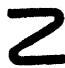
\includegraphics[keepaspectratio]{images/part002_406c0853.jpg}}

应当指出，若 \(f\) 是 \(\mathbf{Y}_1\) 到 \(\mathbf{Y}_2\) 上的双射且一致连续的映射，则它的连续延拓未必是单射，也未必是满射（习题 3）。
% semantic-fragments: legacy-input-seam
\relax{}
\subsection{一致空间的完备化}

定理 3 设 X 是一个一致空间。则存在完备 Hausdorff 一致空间 \(\hat{\mathbf{X}}\) 与一致连续映射 \(i: \mathbf{X} \to \hat{\mathbf{X}}\)，它们具有下列性质：

\begin{enumerate}
\def\labelenumi{(\Alph{enumi})}
\setcounter{enumi}{15}
\tightlist
\item
  给定任意一致连续映射 \(f\)，它把 \(\mathbf{X}\) 映入完备 Hausdorff 一致空间 \(\mathbf{Y}\)，则存在唯一的一致连续映射 \(g: \hat{\mathbf{X}} \to \mathbf{Y}\) 使 \(f = g \circ i\)。
\end{enumerate}

若 \((i_1, X_1)\) 是由完备 Hausdorff 一致空间 \(X_1\) 与具有性质 (P) 的一致连续映射 \(i_1: X \to X_1\) 组成的另一个偶，则存在唯一的同构 \(\varphi: \hat{X} \to X_1\) 使 \(i_1 = \varphi \circ i\)。

定理的第一个断言表明，偶 \((i, \hat{\mathbf{X}})\) 是下列泛映射问题（《集合论》，第四章，§ 3，第 1 目）的解：其中的 \(\Sigma\)-集是完备 Hausdorff 一致空间，\(\sigma\)-态射是一致连续映射，而 \(\alpha\)-映射是 X 到完备 Hausdorff 一致空间中的一致连续映射。于是，偶 \((i, \hat{\mathbf{X}})\) 在相差一个唯一同构的意义下的唯一性由泛映射问题之解的一般性质（同处所引）得出。剩下要证明的是偶 \((i, \hat{\mathbf{X}})\) 的存在性。

\begin{enumerate}
\def\labelenumi{\arabic{enumi})}
\tightlist
\item
  \(\hat{\mathbf{X}}\) 的定义。令 \(\hat{\mathbf{X}}\) 为 \(\mathbf{X}\) 上（第 2 目）极小 Cauchy 滤子全体组成的集。我们要在 \(\hat{\mathbf{X}}\) 上定义一个一致结构。为此，设 \(\mathbf{V}\) 是 \(\mathbf{X}\) 的任一对称一致邻域，令 \(\tilde{\mathbf{V}}\) 表示具有一个公共 V-小集的极小 Cauchy 滤子偶 \((\mathfrak{X}, \mathfrak{Y})\) 全体组成的集。我们将证明，诸集合 \(\tilde{\mathbf{V}}\) 构成 \(\hat{\mathbf{X}}\) 上某个一致结构的一致邻域基本系：
\end{enumerate}

\begin{enumerate}
\def\labelenumi{(\roman{enumi})}
\item
  由于每个 \(\mathcal{X} \in \hat{\mathbf{X}}\) 都是 Cauchy 滤子，按定义我们有 \((\mathcal{X}, \mathcal{X}) \in \tilde{\mathbf{V}}\)，其中 \(\mathbf{V}\) 取遍 \(\mathbf{X}\) 的所有对称一致邻域；因此公理 \((\mathbf{U}_{\mathbf{I}}^{\prime})\) 成立。
\item
  若 V 与 \(V'\) 是 X 的两个对称一致邻域，则 \(W = V \cap V'\) 是对称一致邻域，且每个 W-小的集合也是 V-小的与 \(V'\)-小的；因此 \(\tilde{W} \subset \tilde{V} \cap \tilde{V}'\)，这就证明了 \((B_{I})\)。
\item
  诸集合 \(\tilde{\mathbf{V}}\) 按定义是对称的，因此 \((\mathbf{U}_{\mathbf{II}}^{\prime})\) 成立。（iv）设 \(\mathbf{V}\) 为 \(\mathbf{X}\) 的一个对称一致邻域，\(\mathbf{W}\) 为使 \(\tilde{\mathbf{V}} \subset \mathbf{V}\) 的一个对称一致邻域。考虑三个极小 Cauchy 滤子 \(\mathcal{X}, \mathcal{Y}, \mathfrak{Z}\)，使得 \((\mathcal{X}, \mathcal{Y}) \in \tilde{\mathbf{W}}\) 且 \((\mathcal{Y}, \mathfrak{Z}) \in \tilde{\mathbf{W}}\)；于是存在两个 W-小集 \(\mathbf{M}, \mathbf{N}\)，使 \(\mathbf{M} \in \mathcal{X} \cap \mathcal{Y}\) 且 \(\mathbf{N} \in \mathcal{Y} \cap \mathfrak{Z}\)。由于 \(\mathbf{M}\) 与 \(\mathbf{N}\) 都属于 \(\mathcal{Y}\)，\(\mathbf{M} \cap \mathbf{N}\) 非空，因此（第 1 目命题 1）\(\mathbf{M} \cup \mathbf{N}\) 是 \(\tilde{\mathbf{W}}\)-小的，从而是 V-小的；由于 \(\mathbf{M} \cup \mathbf{N}\) 既属于 \(\mathcal{X}\) 又属于 \(\mathfrak{Z}\)，我们有 \(\tilde{\mathbf{W}} \subset \tilde{\mathbf{V}}\)；因此 \((\mathbf{U}_{\mathbf{III}}^{\prime})\) 成立。
\end{enumerate}

我们接着证明一致空间 \(\hat{\mathbf{X}}\) 是 Hausdorff 的。设 \(\mathcal{X},\mathcal{Y}\) 是 \(\mathbf{X}\) 上两个极小 Cauchy 滤子，使得 \((\mathcal{X},\mathcal{Y})\in \hat{\mathbf{X}}\) 对 \(\mathbf{V}\) 取遍 \(\mathbf{X}\) 的所有对称一致邻域都成立。由此立即得出，诸集合 \(\mathbf{M}\cup \mathbf{N}\)（其中 \(\mathbf{M}\in \mathcal{X}\)、\(\mathbf{N}\in \mathcal{Y}\)）构成一个滤子 \(\mathfrak{Z}\) 的基，该滤子比 \(\mathcal{X}\) 与 \(\mathcal{Y}\) 都粗。现在 \(\mathfrak{Z}\) 是 Cauchy 滤子，因为当 \(\mathbf{V}\) 取遍 \(\mathbf{X}\) 的对称一致邻域时，由假设总存在一个 V-小集 \(\mathbf{P}\)，它同时属于 \(\mathcal{X}\) 与 \(\mathcal{Y}\)，因而属于 \(\mathfrak{Z}\)。由极小 Cauchy 滤子的定义，我们有 \(\mathcal{X} = \mathfrak{Z} = \mathcal{Y}\)，这就表明 \(\hat{\mathbf{X}}\) 是 Hausdorff 的。

\begin{enumerate}
\def\labelenumi{\arabic{enumi})}
\setcounter{enumi}{1}
\item
  \(i\) 的定义；\(\mathbf{X}\) 的一致结构是经由 \(i\) 从 \(\hat{\mathbf{X}}\) 的一致结构取逆像而得的。我们知道，对每个 \(x \in \mathbf{X}\)，邻域滤子 \(\mathfrak{B}(x)\)（\(x\) 在 \(\mathbf{X}\) 中的邻域滤子）是极小 Cauchy 滤子（第 2 目命题 5 推论 1）。于是我们定义 \(i(x) = \mathfrak{B}(x)\)。令 \(f = i \times i\)；我们将证明，对 \(\mathbf{V}\) 取遍 \(\mathbf{X}\) 的每个对称一致邻域，都有 \(\overline{j}(\tilde{\mathbf{V}}) \subset \mathbf{V} \cup \overline{j}[(\mathbf{V})^{\sim}]\)，而这将证明我们的断言（§ 2 第 4 目）。现在，若 \([i(x), i(y)] \in \tilde{\mathbf{V}}\)，则存在一个 V-小集 \(\mathbf{M}\)，它既是 \(x\) 的邻域又是 \(y\) 的邻域，因此 \((x, y) \in \mathbf{V}\)。反之，若 \((x, y) \in \mathbf{V}\)，则立即可见集合 \(\mathbf{V}(x) \cup \mathbf{V}(y)\) 是 \(\overline{\mathbf{V}}\)-小的，且既是 \(x\) 的邻域又是 \(y\) 的邻域。
\item
  \(\hat{\mathbf{X}}\) 是完备的且 \(i(\mathbf{X})\) 在 \(\hat{\mathbf{X}}\) 中稠密。在 \(i(\mathbf{X})\) 上，邻域 \(\tilde{\mathbf{V}}(\mathfrak{X})\)（它是点 \(\mathfrak{X} \in \hat{\mathbf{X}}\) 的邻域）的迹，是使下列关系成立的那些 \(i(x)\) 组成的集：
\end{enumerate}

\[
(\mathcal {X}, i (x)) \in \tilde {\mathbf {V}}.
\]

这个关系意味着，存在 \(x\) 在 X 中的一个 V-小邻域，它属于 \(\mathcal{X}\)，也就是说，\(x\) 是 \(\mathcal{X}\) 的某个 V-小集的内点。令 M 为 \(\mathcal{X}\) 的所有 V-小集的内部之并；则 M 属于 \(\mathcal{X}\)（第 2 目命题 5 推论 4），并且由刚才所说的可得 \(\tilde{\mathrm{V}}(\mathcal{X}) \cap i(\mathrm{X}) = i(\mathrm{M})\)。我们由此断言：

\begin{enumerate}
\def\labelenumi{(\roman{enumi})}
\item
  \(\tilde{\mathbf{V}}(\mathcal{X}) \cap i(\mathbf{X})\) 非空，因此 \(i(\mathbf{X})\) 在 \(\hat{\mathbf{X}}\) 中稠密。
\item
  \(\tilde{\mathbf{V}}(\mathcal{X})\) 在 \(i(\mathbf{X})\) 上的迹属于 X 上的滤子基 \(i(\mathcal{X})\)；因此这个滤子基在 \(\hat{X}\) 中收敛于点 \(\mathfrak{X}\)。
\end{enumerate}

现在设 \(\mathfrak{F}\) 是 \(i(\mathbf{X})\) 上的一个 Cauchy 滤子；则由上面的 2) 及第 1 目命题 4，\(\overline{i}^{1}(\mathfrak{F})\) 是某个 Cauchy 滤子 \(\mathfrak{G}\)（\(\mathbf{X}\) 上的）的基。设 \(\mathfrak{X}\) 是比 \(\mathfrak{G}\) 粗的极小 Cauchy 滤子（第 2 目命题 5）；则 \(i(\mathfrak{X})\) 是 \(i(\mathbf{X})\) 上的一个 Cauchy 滤子基（第 1 目命题 3），且 \(\mathfrak{F}=i[\overline{i}^{1}(\mathfrak{F})]\) 比以 \(i(\mathfrak{X})\) 为基的滤子细。由于后者在 \(\hat{\mathbf{X}}\) 中收敛，\(\mathfrak{F}\) 亦然，于是第 4 目命题 9 表明 \(\hat{\mathbf{X}}\) 是完备的。

\begin{enumerate}
\def\labelenumi{\arabic{enumi})}
\setcounter{enumi}{3}
\tightlist
\item
  性质 (P) 的验证。设 \(f\) 是 \(\mathbf{X}\) 到完备 Hausdorff 一致空间 \(\mathbf{Y}\) 中的一致连续映射。我们先证明，存在唯一的一致连续映射 \(g_{0}: i(\mathbf{X}) \to \mathbf{Y}\) 使 \(f = g_{0} \circ i\)。由于 \(f\) 连续，我们有
\end{enumerate}

\[
f (x) = \lim f (\mathfrak {B} (x)),
\]

因此，若令 \(g_0(i(x)) = \lim f(\mathfrak{V}(x))\)，则我们有 \(f = g_0 \circ i\)；于是剩下要证明 \(g_0\) 在 \(i(\mathbf{X})\) 上一致连续。设 \(\mathbf{U}\) 是 \(\mathbf{Y}\) 的一个一致邻域，\(\mathbf{V}\) 是 \(\mathbf{X}\) 的一个对称一致邻域，使得关系 \((x, x') \in \mathbf{V}\) 蕴含 \((f(x), f(x')) \in \mathbf{U}\)；我们在 2) 中已看到，关系 \((i(x), i(x')) \in \tilde{\mathbf{V}}\) 蕴含 \((x, x') \in \mathbf{V}\)，因而也蕴含

\[
(g _ {0} (i (x)), g _ {0} (i (x ^ {\prime}))) \in \mathbf {U},
\]

这就证明了我们的断言。

设 \(g\) 是 \(g_0\) 由连续性到 \(\hat{\mathbf{X}}\) 上的延拓（第 6 目定理 2）；则 \(f = g \circ i\)，并且显然 \(g\) 是 \(\hat{\mathbf{X}}\) 到 \(Y\) 中满足此关系的唯一连续映射，因为 \(i(\mathbf{X})\) 在 \(\hat{\mathbf{X}}\) 中稠密（第一章 § 8 第 1 目命题 2 推论 1）。

证毕。

定义 4 在定理 3 的证明中所定义的完备 Hausdorff 一致空间 \(\hat{\mathbf{X}}\) 称为 \(\mathbf{X}\) 的 Hausdorff 完备化，而映射 \(i: \mathbf{X} \to \hat{\mathbf{X}}\) 称为 \(\mathbf{X}\) 到其 Hausdorff 完备化中的典范映射。

我们还指出下列事实：

命题 12 （i）子空间 \(i(\mathbf{X})\) 在 \(\hat{\mathbf{X}}\) 中稠密。

\begin{enumerate}
\def\labelenumi{(\roman{enumi})}
\setcounter{enumi}{1}
\item
  等价关系 \(i(x) = i(x')\) 的图像是 \(\mathbf{X}\) 的诸一致邻域之交。
\item
  X 的一致结构是 \(\hat{X}\) 的一致结构在 i 下的逆像{[}或者说是子空间 \(i(\mathbf{X})\) 的一致结构在 i 下的逆像{]}。
\item
  \(i(\mathbf{X})\) 的一致邻域是 X 的一致邻域在 \(i \times i\) 下的像，而在 \(\hat{X} \times \hat{X}\) 中，\(i(\mathbf{X})\) 的一致邻域的闭包构成 \(\hat{X}\) 的一致邻域基本系。
\item
  与 (iii) 已在定理 3 的证明过程中证明；（iv）则由 (i) 与 (iii) 借助于先前证明的一般结果（§ 2 第 4 目的注与命题 6）得出。关系式
\end{enumerate}

\[
i (x) = i \left(x ^ {\prime}\right)
\]

按定义意味着 \(x\) 与 \(x'\) 有相同的邻域滤子。但按定义这就蕴含 \((x, x') \in V\)（其中 \(V\) 是 \(X\) 的任意一致邻域），而其逆是显然的。

推论 若 X 是 Hausdorff 一致空间，则典范映射 \(i: X \to \hat{X}\) 是 X 到 \(\hat{X}\) 的一个稠密子空间上的同构。

当 X 是 Hausdorff 空间时，称 \(\hat{X}\) 为 X 的完备化，并且我们通常借助 i 把 X 与 \(\hat{X}\) 的一个稠密子集等同起来。

注。若作了这一等同，则 X 上的极小 Cauchy 滤子恰好是 \(\hat{X}\) 的点的邻域滤子在 X 上的迹；这由定理 3 的证明得出。

命题 12 的推论刻画了 Hausdorff 一致空间的完备化：

命题 13 若 Y 是完备 Hausdorff 一致空间，且 X 是 Y 的稠密子空间，则典范单射 \(\mathbf{X} \to \mathbf{Y}\) 可延拓为 \(\hat{\mathbf{X}}\) 到 Y 上的一个同构。

因为由第 6 目定理 2，X 到完备 Hausdorff 一致空间 Z 中的每个一致连续映射都唯一地延拓为 Y 到 Z 中的一致连续映射。

命题 14 设 X 是完备 Hausdorff 一致空间，U 是它的一致结构，并设 Z 是 X 的稠密子空间。若 U' 是 X 上的一个比 U 粗、且在 Z 上诱导出与 U 相同的一致结构的一致结构，则 U = U'。

设 \(X'\) 表示集合 \(X\) 赋以一致结构 \(\mathcal{U}'\) 后所得的一致空间。典范映射 \(X' \to \hat{X}'\) 与恒同映射 \(X \to X'\) 的复合是一致连续映射 \(\varphi: X \to \hat{X}'\)。由于 \(Z\) 关于由 \(\mathcal{U}'\) 诱导的一致结构是 Hausdorff 的，\(\varphi\) 在 \(Z\) 上的限制依假设是 \(Z\) 到 \(\varphi(Z)\)（\(\hat{X}'\) 的稠密子空间）上的同构；于是（第 6 目定理 2 的推论）\(\varphi\) 本身是 \(X\) 到 \(\hat{X}'\) 上的同构，因此 \(X' = \hat{X}'\) 且 \(\mathcal{U}' = \mathcal{U}\)。

命题 15 设 X 与 X' 是两个一致空间。对每个一致连续映射 \(f: \mathbf{X} \to \mathbf{X}'\)，存在唯一的一致连续映射 \(\hat{f}: \hat{\mathbf{X}} \to \hat{\mathbf{X}}'\) 使图表

\[
\begin{array}{c}\mathbf {X} \stackrel {{i ^ {\prime}}} {{\to}} \mathbf {X} ^ {\prime}\\i \downarrow \quad \quad \quad \quad \quad \quad \quad \quad \quad \quad \quad \quad \quad \quad \quad \quad \quad \quad \quad \quad \hat {\mathbf {X}} \stackrel {{\rightarrow}} {{\longrightarrow}} \hat {\mathbf {X}} ^ {\prime}\\f\end{array}
\]

可交换 (*)，其中 \(i: \mathbf{X} \to \hat{\mathbf{X}}\) 与 \(i': \mathbf{X}' \to \hat{\mathbf{X}}'\) 是典范映射。

对函数 \(i' \circ f: \mathbf{X} \to \hat{\mathbf{X}}'\) 应用定理 3。

推论 若 \(f: \mathbf{X} \to \mathbf{X}'\) 与 \(g: \mathbf{X}' \to \mathbf{X}''\) 是两个一致连续映射，且 \(h = g \circ f\)，则 \(\hat{h} = \hat{g} \circ \hat{f}\)。

这是命题 15 中唯一性的直接推论。

\subsection{一致空间的伴随 Hausdorff 一致空间}

命题 16 设 X 是一致空间，i 是 X 到其 Hausdorff 完备化 \(\hat{\mathbf{X}}\) 中的典范映射。对 X 到 Hausdorff 一致空间 Y 中的每个一致连续映射 \(f\)，存在唯一的一致连续映射 \(h: i(\mathbf{X}) \to \mathbf{Y}\) 使 \(f = h \circ i\)。

我们可以把 Y 与其完备化 \(\hat{Y}\) 的一个子空间等同起来（第 7 目命题 12 的推论），于是 f 可看作 X 到 \(\hat{Y}\) 中的一致连续映射。由定理 3，f 这时具有形式 \(f = g \circ i\)，其中 g 是 \(\hat{X}\) 到 \(\hat{Y}\) 中的一致连续映射。若 h 是 g 在 \(i(X)\) 上的限制，则显然 \(f = h \circ i\)，且 h 把 \(i(X)\) 映到 Y 中。h 的唯一性是显然的。

因此，偶 \((i, i(X))\) 是某个泛映射问题（《集合论》，第四章，§ 3，第 1 目）的解，这次我们取 \(\Sigma\)-集为 Hausdorff 一致空间，取 \(\sigma\)-态射（相应地 \(\alpha\)-映射）为一致连续映射（相应地，X 到 Hausdorff 一致空间中的一致连续映射）。

定义 5 在定理 3 的证明中所定义的 Hausdorff 一致空间 \(i(\mathbf{X})\) 称为 \(\mathbf{X}\) 的伴随 Hausdorff 一致空间。

于是，X 的 Hausdorff 完备化就是 X 的伴随 Hausdorff 一致空间的完备化。

推论 设 X、Y 是两个一致空间，\(X'\)、\(Y'\) 是它们的伴随 Hausdorff 空间。对每个一致连续映射 \(f: X \to Y\)，存在唯一的一致连续映射 \(f': X' \to Y'\) 使图表

\pandocbounded{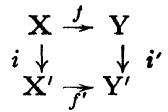
\includegraphics[keepaspectratio]{images/part002_3c8eaa6f.jpg}}

可交换，其中 \(i\) 与 \(i'\) 是典范映射。

对 \(i' \circ f: \mathbf{X} \to \mathbf{Y}'\) 应用命题 16。

一致空间的伴随 Hausdorff 空间也可以用下列性质来刻画：

命题 17 设 X 是一致空间，\(i(X)\) 是它的伴随 Hausdorff 空间，并设 \(f\) 是 X 到 Hausdorff 一致空间 \(X'\) 上的映射，使得 X 的一致结构是经由 \(f\) 从 \(X'\) 的一致结构取逆像而得的。则映射 \(g:i(X)\to X'\)（它使 \(f=g\circ i\)）是一个同构。

由命题 16，g 一致连续；g 显然是满射，并且也是单射，因为关系 \(f(x) = f(y)\) 按定义蕴含 \((x,y)\) 属于 X 的所有一致邻域，从而 \(i(x)=i(y)\)（第 7 目命题 12）。最后，\(X'\) 的一致邻域是 X 的一致邻域在 \(f\times f\) 下的像（§ 2 第 4 目的注），因而它们也是经由 \(g\times g\) 从 \(i(\mathbf{X})\) 的一致邻域得到的像（第 7 目命题 12）；由此即得结论。

注。设 R 是 X 上的等价关系 \(i(x) = i(x')\)。我们已看到（第 7 目命题 12），R 的图像 C 是 X 的所有一致邻域之交。显然，X 中的每个开集（因而每个闭集）关于 R 是饱和的；考虑到拓扑的逆像的定义，我们断言，商空间 X/R 到 \(i(X)\) 上的典范双射（由 \(i\) 所诱导）是一个同胚。因此，作为拓扑空间，X 的伴随 Hausdorff 空间可与 X/R 等同。典范映射 \(i: X \to i(X)\) 是开的和闭的，甚至是逆紧的（第一章 § 10 第 2 目的例）。

设 \(X'\) 是另一个一致空间，\(C'\) 是 \(X'\) 的所有一致邻域之交，\(R'\) 是以 \(C'\) 为图像的等价关系。设 \(f: X \to X'\) 是连续映射。由于在 \(f\) 之下，\(f(x)\) 的任一邻域的逆像是 \(x\) 的邻域，可知在 \(f\) 之下 \(C'(f(x))\) 的逆像包含 \(C(x)\)，因此 \(f\) 与 \(R\) 及 \(R'\) 相容，并诱导出一个连续映射 \(X/R \to X'/R'\)（第一章 § 3 第 4 目命题 6 的推论）。这推广了命题 16 的推论。

\subsection{子空间与积空间的完备化}

命题 18 设 X 是一个集合，\((\mathbf{Y}_{\lambda})_{\lambda \in \mathbf{L}}\) 是一族一致空间，且对每个 \(\lambda \in \mathbf{L}\)，设 \(f_{\lambda}\) 是 X 到 \(\mathbf{Y}_{\lambda}\) 中的映射。设 X 赋有最粗的一致结构 \(\mathcal{U}\)，它使所有 \(f_{\lambda}\) 都一致连续。则 X 的 Hausdorff 完备化 \(\hat{\mathbf{X}}\) 的一致结构是使所有映射 \(\hat{f}_{\lambda} \colon \hat{\mathbf{X}} \to \hat{\mathbf{Y}}_{\lambda} (\lambda \in \mathbf{L})\)（第 7 目命题 15）都一致连续的最粗的一致结构。此外，若 \(j_{\lambda}\) 是 \(\mathbf{Y}_{\lambda}\) 到 \(\hat{\mathbf{Y}}_{\lambda}\) 中的典范映射，且 \(g_{\lambda} = j_{\lambda} \circ f_{\lambda}\)，则 \(\hat{\mathbf{X}}\) 可与 \(\prod_{\lambda \in \mathbf{L}} \hat{\mathbf{Y}}_{\lambda}\) 中 X 在映射 \(x \to (g_{\lambda}(x))\) 下的像的闭包等同起来。

设 \(X'\)（相应地 \(Y_{\lambda}'\)）是 \(X\)（相应地 \(Y_{\lambda}\)）的伴随 Hausdorff 一致空间，并设 \(f_{\lambda}' \colon X' \to Y_{\lambda}'\) 是使图表

\[
\begin{array}{c} \mathbf {X} \xrightarrow {f _ {\lambda}} \mathbf {Y} _ {\lambda} \\ i \downarrow \\ \mathbf {X ^ {\prime}} \xrightarrow [ f _ {j} ^ {I} ]{} \mathbf {Y} _ {\lambda} ^ {\prime} \end{array}
\]

可交换的一致连续映射（i 为典范映射）。

初始一致结构的传递性（§ 2 第 3 目命题 5）一方面表明，\(\mathcal{U}\) 是使映射 \(j_{\lambda} \circ f_{\lambda}: \mathbf{X} \to \mathbf{Y}_{\lambda}'\) 都一致连续的最粗一致结构；另一方面表明，\(\mathcal{U}\) 也是经由 \(i\) 从 \(\mathcal{U}'\)（即集合 \(\mathbf{X}'\) 上使诸 \(f_{\lambda}'\) 一致连续的最粗一致结构）取逆像而得。现在 \(\mathcal{U}'\) 是 Hausdorff 的，因为若 \(x_{1}, x_{2}\) 是 \(\mathbf{X}\) 的两点，使得 \(j_{\lambda}(f_{\lambda}(x_{1})) = j_{\lambda}(f_{\lambda}(x_{2}))\) 对每个 \(\lambda \in L\) 成立，则 \((x_{1}, x_{2})\) 属于 \(\mathcal{U}\) 的所有一致邻域，从而 \(i(x_{1}) = i(x_{2})\)。于是第 8 目命题 17 表明，\(\mathcal{U}'\) 是伴随 Hausdorff 空间 \(\mathbf{X}'\)（\(\mathbf{X}\) 的）的一致结构。

在此情形下，双射 \(x' \to (f_{\lambda}'(x'))\) 把 X 等同于积 \(\prod_{\lambda} Y_{\lambda}'\) 的一个一致子空间（ \(\S\) 2 第 6 目命题 8）。由于诸 \(Y_{\lambda}'\) 是 Hausdorff 的，每个 \(Y_{\lambda}'\) 可与其完备化 \(\hat{Y}_{\lambda}\) 的一个稠密子空间等同，从而 \(\prod_{\lambda} Y_{\lambda}'\) 可与 \(\prod_{\lambda} \hat{Y}_{\lambda}\) 的一个稠密子空间等同（第一章 § 4 第 3 目命题 7）。但 \(\prod_{\lambda} \hat{Y}_{\lambda}\) 是 Hausdorff 的且完备的（第 5 目命题 10）；因此闭包 \(\overline{X}'\)（即 \(X'\) 在 \(\prod_{\lambda} \hat{Y}_{\lambda}\) 中的闭包）是完备 Hausdorff 子空间（第 4 目命题 8），它可与 X 的 Hausdorff 完备化 \(\hat{X}\) 等同；在这一等同之下，诸映射 \(\hat{f}_{\lambda}\) 成为到因子 \(\hat{Y}_{\lambda}\) 上的投影，命题得证。

推论 1 设 X 是一致空间，i 是 X 到其 Hausdorff 完备化 \(\hat{X}\) 中的典范映射；设 A 是 X 的子空间，j: A → X 是典范单射。则 j: \(\hat{A} \rightarrow \hat{X}\) 是 \(\hat{A}\) 到 i(A) 在 \(\hat{X}\) 中的闭包上的一个同构。

推论 2 设 \((\mathbf{Y}_{\lambda})_{\lambda \in \mathbf{L}}\) 是一族一致空间。则积空间 \(\prod_{\lambda \in \mathbf{L}}\mathbf{Y}_{\lambda}\) 的 Hausdorff 完备化典范地同构于积 \(\prod_{\lambda \in \mathbf{L}}\hat{\mathbf{Y}}_{\lambda}\)。

\section{一致空间与紧空间之间的关系}

\subsection{紧空间的一致结构}

定义 1 拓扑空间 X 上的一致结构称为与 X 的拓扑相容，如果后者与该一致结构诱导的拓扑重合。

若拓扑空间上存在与它的拓扑相容的一致结构，则称该拓扑空间为可一致化的，并称其拓扑为可一致化的。

存在不可一致化的拓扑空间，例如任何不满足公理 \((\mathrm{O}_{\mathrm{III}})\) 的空间（§ 1 第 2 目命题 2 的推论 3）；于是就产生了在什么条件下一个拓扑空间可一致化的问题。

我们要到第九章 § 1 才给出这个问题的完整回答。在本节中我们只考察一个重要的特殊情形，即 X 是紧空间的情形。这时我们有下面的定理：

定理 1 在紧空间 X 上，恰有一个与 X 的拓扑相容的一致结构；这个一致结构的一致邻域是对角线 \(\Delta\)（在 \(\mathbf{X} \times \mathbf{X}\) 中的）的所有邻域。此外，赋有这个一致结构的 X 是完备一致空间。

定理的最后一部分是直接的；因为 X 上的每个 Cauchy 滤子都有聚点{[}公理 (C){]}，因而收敛（§ 3 第 2 目命题 5 推论 2）。

我们接着证明，若 X 上存在与 X 的拓扑相容的一致结构，则它的一致邻域组成的集 U 是 \(\Delta\) 的所有邻域组成的集。我们已知每个一致邻域都是 \(\Delta\) 的邻域（§ 1 第 2 目命题 2），因此只需证明反之每个 \(\Delta\) 的邻域都属于 U。假设存在 \(\Delta\) 的一个不属于 U 的邻域 U；则当 V 取遍 U 时，诸集合 \(V \cap CU\) 构成紧空间 \(X \times X\) 上一个滤子 G 的基；于是 G 有一个聚点 \((a, b)\)（不属于 \(\Delta\)）。由于 U 是比 G 粗的滤子，\((a, b)\) 也是 U 的聚点。但按假设由 U 定义的一致结构是 Hausdorff 的；因此 U 的诸集合的闭包之交是 \(\Delta\)（§ 1 第 2 目命题 2 的推论 2 及命题 3）；于是我们得到矛盾。

因此剩下要证明的是，\(\mathfrak{B}\)（即 \(\Delta\) 在 \(\mathbf{X} \times \mathbf{X}\) 中的邻域组成的集）是某个与 \(\mathbf{X}\) 的拓扑相容的一致结构的一致邻域集。为此只需证明 \(\mathfrak{B}\) 是 \(\mathbf{X}\) 上某个 Hausdorff 一致结构的一致邻域集；因为这时该一致结构诱导的拓扑将比 \(\mathbf{X}\) 的拓扑粗（第一章 § 2 第 2 目命题 3），从而必与后者重合（第一章 § 9 第 4 目定理 2 推论 3）。

\(\mathfrak{B}\) 显然满足公理 \((\mathbf{F}_{\mathrm{I}})\) 与 \((\mathbf{F}_{\mathrm{II}})\)。我们来证明公理 \((\mathbf{U}_{\mathrm{II}})\) 与 \((\mathbf{U}_{\mathrm{III}})\) 也得到满足，并且 \(\Delta\) 是 \(\mathfrak{B}\) 中诸集合之交。先证最后一点：每个由单独一点 \((x, y) \in \mathbf{X} \times \mathbf{X}\) 组成的集合都是闭的，因为 \(\mathbf{X}\) 是 Hausdorff 的；因此若 \(x \neq y\)，则 \((x, y)\) 在 \(\mathbf{X} \times \mathbf{X}\) 中的余集是 \(\Delta\) 的邻域。由于对称映射 \((x, y) \to (y, x)\) 是 \(\mathbf{X} \times \mathbf{X}\) 到自身的同胚，可知 \(V \in B\) 蕴含 \(\overline{V} \in B\)，由此得 \((U_{II})\)。最后，假设 \((U_{III})\) 不满足；则存在集合 \(V \in B\)，使得对所有 \(W \in B\)，集合 \(\overline{W} \cap C V\) 非空；于是当 W 取遍 B 时，诸集合 \(\overline{W} \cap C V\) 构成 \(X \times X\) 上的一个滤子基，且该滤子基有一个聚点 \((x, y)\)（不在 \(\Delta\) 中）。现在，由于 X 是正则的（第一章 §9 第 2 目命题 1 的推论），存在不相交的开邻域 \(U_{1}\)（x 的）与 \(U_{2}\)（y 的），并且存在闭邻域 \(V_{1} \subset U_{1}\) 与 \(V_{2} \subset U_{2}\)（分别为 x 与 y 的闭邻域）。令 \(U_{3} = C(V_{1} \cup V_{2})\)，并考虑邻域

\[
\mathbf {W} = \bigcup_ {i = 1, 2, 3} (\mathrm{U} _ {i} \times \mathrm{U} _ {i}) \text {of} \Delta \text {in} \mathbf {X} \times \mathbf {X}.
\]

由这些定义立即得出，若 \((u, v) \in W\) 且 \(u \in V_1\)（相应地 \(u \in U_1\)），则必有 \(v \in U_1\)（相应地 \(v \in U_1 \cup U_3 = \complement V_2\)）；因此邻域 \(V_1 \times V_2\)（\((x, y)\) 在 \(X \times X\) 中的）不与 \(W\) 相交，这就得到矛盾。证明完毕。

注 1 对每个有限开覆盖 \(\Re = (\mathrm{U}_i)_{1\leqslant i\leqslant n}\)（\(\mathbf{X}\) 的），集合

\[
\mathrm{V} _ {\Re} = \bigcup_ {i = 1} ^ {n} \left(\mathrm{U} _ {i} \times \mathrm{U} _ {i}\right)
\]

是 \(\Delta\)（在 \(\mathbf{X} \times \mathbf{X}\) 中的）的邻域，并且这些集合 \(\mathrm{V}_{\Re}\) 构成 \(\Delta\) 的一个基本邻域系（因而构成 \(\mathbf{X}\) 上唯一一致结构的一致邻域基本系）。设 \(\mathbf{W}\) 是 \(\Delta\) 在 \(\mathbf{X} \times \mathbf{X}\) 中的任一邻域；则对每个 \(x \in \mathbf{X}\)，存在开邻域 \(\mathbf{U}_x\)（\(x\) 在 \(\mathbf{X}\) 中的），使 \(\mathbf{U}_x \times \mathbf{U}_x \subset \mathbf{W}\)。由于诸 \(\mathbf{U}_x\)（ \(x \in \mathbf{X}\) ）构成 \(\mathbf{X}\) 的开覆盖，故存在有限多个点 \(x_i\)（ \(1 \leqslant i \leqslant n\) ）使诸 \(\mathbf{U}_{x_i}\)（ \(1 \leqslant i \leqslant n\) ）构成一个覆盖 \(\Re\)（\(\mathbf{X}\) 的）。于是有 \(\mathrm{V}_{\Re} \subset \mathrm{W}\)，这就证明了所述断言。

由于这个原因，X 上唯一的一致结构常称为有限开覆盖的一致结构（参看第九章 § 4 习题 17）。

推论 1 紧空间的每个子空间都是可一致化的。

推论 2 每个局部紧空间都是可一致化的。

因为由 Alexandroff 定理（第一章 § 9 第 8 目定理 4），局部紧空间同胚于紧空间的子空间。

注 2 可能发生这样的情形：与局部紧空间的拓扑相容的一致结构不止一个且互不相同。

例如，我们已经看到，在无限离散空间上，有多于一个相容于离散拓扑的不同一致结构（§ 2 第 2 目的注）。

尽管如此，与可一致化空间的拓扑相容的一致结构的唯一性并不是刻画紧空间的性质；存在不紧但其一致结构唯一的局部紧空间（习题 4）。

定理 2 每个连续映射 \(f\)（从紧空间 \(X\) 到一致空间 \(X'\) 中的）都是一致连续的。

令 \(g = f \times f\)，则 \(g\) 在 \(X \times X\) 上连续（第一章 § 4 第 1 目命题 1 推论 1）；因此对每个开一致邻域 \(V'\)（\(X'\) 的），\(\overline{g}(V')\) 是 \(X \times X\) 的开子集，它显然包含对角线。于是定理由定理 1 得出，因为 \(X'\) 的开一致邻域构成一个一致邻域基本系（§ 1 第 2 目命题 2 推论 2）。

在定理 2 的假设下，\(f\) 在任一子空间 \(A\)（\(X\) 的）上的限制是一致连续的；因此（§ 3 第 6 目定理 2）：

推论 设 A 是紧空间 X 的稠密子空间，f 是 A 到完备 Hausdorff 一致空间 X' 中的映射。则 f 可由连续性延拓到整个 X 上，当且仅当 f 一致连续。

\subsection{一致空间的紧性}

定义 2 一致空间 X 称为准紧的，如果它的 Hausdorff 完备化 \(\hat{\mathbf{X}}\) 是紧的。一致空间 X 的子集 A 称为准紧子集，如果 X 的一致子空间 A 是准紧的。

于是，一致空间 X 的子集 A 是准紧的，当且仅当 \(i(\mathbf{A})\) 在 \(\hat{X}\) 中的闭包是紧的（ \(i: X \rightarrow \hat{X}\) 为典范映射）（ \(\S\) 3 第 9 目命题 18 推论 1）。

例。在任何一致空间 X 中，Cauchy 序列 \((x_{n})\) 的点组成的集是准紧的。由于诸 \(x_{n}\) 在 \(\hat{X}\) 中的像仍构成 Cauchy 序列，我们可以假定 X 是 Hausdorff 的；于是在 \(\hat{X}\) 中，由诸点 \(x_{n}\) 组成的集的闭包由诸点 \(x_{n}\) 与 \(\lim_{n\to\infty}x_{n}\) 组成，因而是紧的（第一章 § 9 第 3 目例 2）。

定理 3 一致空间 X 是准紧的，当且仅当对 X 的每个一致邻域 V，存在 X 的一个由 V-小集组成的有限覆盖。

我们可以更直观地把这个条件表述为：X 可以被有限多个集覆盖，而这些集要多么小就可以多么小。

设 \(i: \mathbf{X} \to \hat{\mathbf{X}}\) 为典范映射，则 \(\mathbf{X}\) 的一致邻域是经由 \(i \times i\) 从 \(\hat{\mathbf{X}}\) 的一致邻域取逆像而得的集合（§ 3 第 7 目命题 12）。设 \(\mathbf{X}\) 准紧，并设 \(\mathbf{U}\) 为任一一致邻域（\(\hat{\mathbf{X}}\) 的）；则存在一个对称一致邻域 \(\mathbf{U}'\)（\(\hat{\mathbf{X}}\) 的），使 \(\hat{\mathbf{U}}' \subset \mathbf{U}\)。由于 \(\hat{\mathbf{X}}\) 是紧的，存在有限多个点 \(x_j \in \hat{\mathbf{X}}\) 使诸 \(\mathbf{U}'(x_j)\)（它们是 U-小集）覆盖 \(\hat{\mathbf{X}}\)。若 \(\mathbf{V}\) 是 \(\mathbf{U}\) 经由 \(i \times i\) 的逆像，则诸集合 \(i^{-1}(\mathbf{U}'(x_j))\) 是 V-小集且覆盖 \(\mathbf{X}\)。反之，假设对每个一致邻域 \(\mathbf{V}\)（\(\mathbf{X}\) 的），存在 \(\mathbf{X}\) 的一个由 V-小集组成的有限覆盖。我们要证明每个超滤子 \(\mathfrak{F}\)（\(\hat{\mathbf{X}}\) 上的）都收敛；由于 \(\hat{\mathbf{X}}\) 是完备的，只需证明 \(\mathfrak{F}\) 是 Cauchy 滤子，即对每个闭一致邻域 \(\mathbf{U}\)（\(\hat{\mathbf{X}}\) 的），在 \(\mathfrak{F}\) 中有一个 U-小集（§ 1 第 2 目命题 2 推论 2）。设 \(\mathbf{V}\) 是 \(\mathbf{U}\) 在 \(i \times i\) 下的逆像，并设 \((\mathbf{B}_j)\) 是 \(\mathbf{X}\) 的一个由 V-小集组成的有限覆盖；则诸集合 \(C_j = i(B_j)\) 是 U-小集且覆盖 \(i(\mathbf{X})\)，于是

\[
\hat {\mathbf {X}} = \bigcup_ {j} \overline {{\mathbf {C}}} _ {j}.
\]

另一方面，由于 \(\mathbf{C}_j \times \mathbf{C}_j \subset \mathbf{U}\)，且 \(\mathbf{U}\) 在 \(\hat{\mathbf{X}} \times \hat{\mathbf{X}}\) 中是闭的，故 \(\overline{\mathbf{C}}_j \times \overline{\mathbf{C}}_j \subset \mathbf{U}\)，从而诸 \(\overline{\mathbf{C}}_j\) 也是 \(\mathbf{U}\)-小集。由于 \(\mathfrak{F}\) 是超滤子，诸 \(\overline{\mathbf{C}}_j\) 之一属于 \(\mathfrak{F}\)（第一章 § 6 第 4 目命题 5 的推论）。

证毕。

推论 一致空间 X 是紧的，当且仅当它是 Hausdorff 的、完备的，并且能被有限多个 V-小集覆盖，其中 V 是 X 的任一一致邻域。

这由定理 3 及第 1 目的定理 1 得出。

注 1 非 Hausdorff 的拟紧空间未必可一致化，因为它未必满足公理 (O \(_{III}\) )（参看第一章 § 9 第 2 目）；例如代数几何中出现的大多数非 Hausdorff 拟紧空间都不满足公理 (O \(_{III}\) )（参看习题 2）。

命题 1 在一致空间中，准紧集的每个子集、准紧集的每个有限并以及每个准紧集的闭包都是准紧的。

前两个断言是定理 3 的直接推论。设 X 是一致空间，A 是 X 的准紧子集，并设 \(i: \mathbf{X} \to \hat{\mathbf{X}}\) 为典范映射。\(i(\overline{\mathbf{A}})\) 包含在 \(i(\mathbf{A})\) 于 \(\hat{\mathbf{X}}\) 中的闭包内（第一章 § 2 第 1 目定理 1），因此 \(i(\overline{\mathbf{A}})\) 在 \(\hat{\mathbf{X}}\) 中的闭包包含在一个紧集中，从而是紧的。

\pandocbounded{
\includegraphics[keepaspectratio]{images/part002_3e3611b3.jpg}}

注 2 在一致空间 X 中，相对紧集 A 是准紧的，因为 A 包含在一个紧集中。另一方面，即使 X 是 Hausdorff 的，准紧集也未必在 X 中相对紧，X 本身准紧但不紧的情形就表明了这一点。

命题 2 设 \(f: \mathbf{X} \to \mathbf{Y}\) 是一致连续映射。若 \(\mathbf{A}\) 是 \(\mathbf{X}\) 的任一准紧子集，则 \(f(\mathbf{A})\) 是 \(\mathbf{Y}\) 的准紧子集。因为若 \(i: \mathbf{X} \to \hat{\mathbf{X}}\) 与 \(j: \mathbf{Y} \to \hat{\mathbf{Y}}\) 为典范映射，我们有 \(j(f(\mathbf{A})) = \hat{f}(i(\mathbf{A}))\)（§ 3 第 7 目命题 15），因而 \(j(f(\mathbf{A}))\) 在 \(\hat{\mathbf{Y}}\) 中相对紧（第一章 § 9 第 4 目定理 2 推论 1）。

命题 3 设 X 是一个集合，\((\mathrm{Y}_{\lambda})_{\lambda \in \mathbf{L}}\) 是一族一致空间，且对每个 \(\lambda \in L\)，设 \(f_{\lambda}\) 是 X 到 \(Y_{\lambda}\) 中的映射。设 X 赋有使诸 \(f_{\lambda}\) 一致连续的最粗一致结构。则 X 的子集 A 是准紧的，当且仅当 \(f_{\lambda}(A)\) 是 \(Y_{\lambda}\) 的准紧子集（对每个 \(\lambda \in L\)）。

这个条件由命题 2 知是必要的。充分性由 § 3 第 9 目命题 18 给出的 X 的 Hausdorff 完备化的刻画以及 Tychonoff 定理（第一章 § 9 定理 3 的推论）得出。

\subsection{一致空间中的紧集}

下面这个关于任意一致空间的命题，是第一章 § 9 第 2 目命题 2 对紧空间的更精确形式。

命题 4 在一致空间 X 中，设 A 是紧集，B 是闭集，且 A∩B=∅。则存在 X 的一致邻域 V，使 V(A) 与 V(B) 不相交。

若命题不真，则当 V 取遍 X 的对称一致邻域时，诸集合 \(A \cap \mathring{V}(B)\) 都不空；于是这些集合将在 A 上构成一个滤子基，它有一个聚点 \(x_0 \in A\)。因此对每个对称一致邻域 \(V\)（\(X\) 的），\(\dot{V}(x_0)\) 将与 \(B\) 相交，从而由于 \(B\) 是闭的，应有 \(x_0 \in B\)，与假设矛盾。

推论 设 A 是一致空间 X 中的紧集；则当 V 取遍 X 的一致邻域时，诸集合 V(A) 构成 A 的一个基本邻域系。

设 U 是 A 的任一开邻域，则 B = CU 是闭的且不与 A 相交；于是由命题 4，存在一致邻域 V 使 \(\mathrm{V}(\mathrm{A}) \cap \mathrm{V}(\mathrm{B}) = \varnothing\)，因此 \(\mathrm{V}(\mathrm{A}) \subset \mathrm{U}\)。

\subsection{紧空间中的连通集}

定义 3 设 V 是一致空间 X 的对称一致邻域。X 的点的有限序列 \((x_{i})_{0\leqslant i\leqslant n}\) 称为一条 V-链，如果 \(x_{i}\) 与 \(x_{i+1}\) 对 \(0\leqslant i<n\) 是 V-邻近的。点 \(x_{0}\) 与 \(x_{n}\) 称为该 V-链的端点，并称它们由这条 V-链连接。

给定对称一致邻域 V，关系“存在一条连接 x 与 y 的 V-链”是 X 中 x 与 y 之间的一个等价关系。设 \(A_{x,v}\) 是 x 关于这个关系的等价类，即可由一条 V-链与 x 连接的所有 \(y \in X\) 组成的集。显然，若 \(y \in A_{x,v}\)，则 \(\mathrm{V}(y) \subset \mathrm{A}_{x,\mathrm{v}}\)；因此 \(A_{x,v}\) 在 X 中是开的；而 \(A_{x,v}\) 的余集作为一些等价类的并，也是开的。于是：

命题 5 在一致空间 X 中，可与给定点 x 由 V-链连接的点组成的集 \(A_{x,v}\) 在 X 中既开又闭。

对每个 \(x \in X\)，设 \(A_{x}\) 表示当 V 取遍 X 的对称一致邻域时诸集合 \(A_{x,v}\) 的交；\(A_{x}\) 是 x 关于等价关系“对一切对称一致邻域 V，存在一条连接 x 与 y 的 V-链”的等价类。

命题 6 在紧空间 X 中，x 的连通分支、集合 \(A_{x}\)、以及 x 的既开又闭的邻域的交，这三者是同一个集合。

只需证明 \(A_{x}\) 是连通的：因为在任意一致空间 X 中，x 的连通分支包含在 x 的既开又闭的邻域的交中，而这个交由命题 5 包含在 \(A_{x}\) 中。

假设 \(A_{x}\) 不连通。由于 \(A_{x}\) 是闭的，存在两个不相交的非空闭集 B 与 C，使 \(B \cup C = A_{x}\)。由 §3 的命题 4，存在 X 的一致邻域 U 使 \(U(B) \cap U(C)\) 为空。

设 W 是开的一致邻域，使 \(\hat{W} \subset U\)，并设 H 是闭集，即 \(W(B) \cup W(C)\) 在 X 中的余集。例如设 \(x \in B\)，并设 y 是 C 的一点。则对每个对称一致邻域 \(V \subset W\)，由 W 的取法，对 i 用归纳法立即看出，在 X 中连接 x 与 y 的每条 V-链 \((x_{i})_{0 \leqslant i \leqslant n}\) 必有一点在 H 中。由于按假设对每个对称一致邻域 V，x 与 y 都可由一条 V-链连接，可见 \(H \cap A_{x,v}\) 当 \(V \subset W\) 时不空。另一方面，若 \(V' \subset V\)，则显然 \(A_{x,v'} \subset A_{x,v}\)；由此可得，当 V 取遍 X 的对称一致邻域时，诸集合 \(H \cap A_{x,v}\) 在紧空间 H 中构成一个由闭集组成的滤子基。因此所有这些集合有一公共点，从而 H 与 \(A_{x}\) 相交；但这与 H 的定义矛盾。

推论 设 X 是局部紧空间，K 是 X 的紧连通分支。则 K 的既开又闭的邻域构成 K 的一个基本邻域系。

设 V 是 K 在 X 中的相对紧开邻域（第一章 § 9 第 7 目命题 10），并设 F 是它的边界。设 U ⊂ V 是一个关于 V 既开又闭的集合。则 U 在 X 中是闭的，且若此外 U 不与 F 相交，则 U 在 X 中是开的（因为这时 U ⊂ V 且 U 在 V 中是开的）。因此只需证明存在 V 的一个子集，它包含 K、不与 F 相交且关于 V 既开又闭。

假设情形不是这样：则 F 与 \(\overline{V}\) 的那些包含 K 且在 \(\overline{V}\) 中既开又闭的子集的交，在 F 中构成一个由闭集组成的滤子基；F 是紧的，故这些集合有一公共点 \(y \in F\)。但这是荒谬的；由于 \(\overline{V}\) 是紧的，K 是 \(\overline{V}\) 的一个连通分支，且由命题 6，\(\overline{V}\) 中那些包含 K 且既开又闭的集合的交恰好是 K。推论至此得证。

命题 7 设 X 是紧空间，R 是 X 上的等价关系，其类是 X 的连通分支。则商空间 X/R 是紧的且全不连通。

由第一章 § II 第 5 目命题 9 我们知道 X/R 是全不连通的；因此要证明 X/R 是 Hausdorff 的（第一章 § 10 第 4 目命题 8）。设 A 与 B 是 X 的两个不同的连通分支。由命题 6，存在 X 的对称一致邻域 U，使 A 的任何点都不能由一条 U-链与 B 的任何点连接。X 中可由一条 U-链与一点 \(x \in A\)（相应地 \(y \in B\)）连接的点组成的集 V（相应地 W）在 X 中既开又闭（命题 5）且包含 A（相应地 B）；因此这两个集合分别是 A 与 B 的开邻域，关于 R 是饱和的，且不相交。证明完毕。

\BourbakiExercises

\BourbakiExerciseGroup

\begin{enumerate}
\def\labelenumi{\arabic{enumi})}
\tightlist
\item
  设 X 是无限集，F 是 X 上的一个超滤子，且 F 中诸集之交为空。对每个 \(A \in F\)，设 \(V_{A}\) 表示子集 \(\Delta \cup (A \times A)\)（\(X \times X\) 的）。证明：当 A 取遍 F 时，诸集合 \(V_{A}\) 构成 X 上某个一致结构 \(\mathcal{U}(\mathfrak{F})\) 的一致邻域基本系，且该一致结构诱导的拓扑是离散拓扑。
\end{enumerate}

*2) 在带有加法一致结构的实直线 R 上，证明当 V 取遍 R 的一致邻域滤子时，诸集合 V(Z) 并不构成有理整数集 Z 的基本邻域系。*（参看 § 4 第 3 目命题 4 的推论）。

*3) 设 V 是 R 上加法一致结构中由所有对 \((x, y)\)（满足 \(|x - y| \leqslant 1\) 或 \(xy \geqslant 1\) 的）组成的一致邻域。证明 V 在 \(R \times R\) 中是闭的，但若 A 表示由所有整数 \(n \geqslant 2\) 组成的 R 的（闭）子集，则 \(V(A)\) 在 \(R\) 中不是闭的。*

\begin{enumerate}
\def\labelenumi{\arabic{enumi})}
\setcounter{enumi}{3}
\tightlist
\item
  证明若一致空间是 Kolmogoroff 空间（第一章 § 1 习题 2），则它是 Hausdorff 的。
\end{enumerate}

¶ 5) a) 设 X 是一致空间，U 是它的一致结构；对 X 的每个一致邻域 V，设 \(\tilde{V}\) 是 \(\mathfrak{P}(X) \times \mathfrak{P}(X)\) 的子集，由 X 的子集的所有满足 \(M \subset V(N)\) 且 \(N \subset V(M)\) 的对 (M, N) 组成。证明诸集合 \(\tilde{V}\) 构成某个一致结构 \(\tilde{U}\)（\(\mathfrak{P}(X)\) 上的）的一致邻域基本系。

\begin{enumerate}
\def\labelenumi{\alph{enumi})}
\setcounter{enumi}{1}
\item
  在集 \(\mathfrak{P}_{0}(\mathbf{X})\)（由 \(\mathbf{X}\) 的非空子集组成）上，证明由拓扑 \(\mathfrak{C}(\tilde{\mathcal{U}})\)（它由 \(\tilde{\mathcal{U}}\) 诱导）所诱导的拓扑比拓扑 \(\mathfrak{C}_{\Phi}\) 细（第一章 § 2 习题 7）。
\item
  若 X 至少有两点且 U 是 Hausdorff 的，证明 \(\mathfrak{G}(\tilde{\mathcal{U}})\) 在 \(\mathfrak{P}_{0}(\mathbf{X})\) 上诱导的拓扑决不比 \(G_{\Omega}\) 粗。\(\mathfrak{G}(\tilde{\mathcal{U}})\) 在由 X 的非空闭子集组成的集 \(\mathfrak{F}(\mathbf{X})\) 上诱导的拓扑比 \(G_{\Omega}\) 在这个集上诱导的拓扑细，当且仅当对 X 的每个闭子集 A，当 V 取遍 X 的一致邻域时诸集合 V(A) 构成 A 的一个基本邻域系。
\end{enumerate}

*d) 证明在第一章 § 11 习题 18 定义的商集 X/R 上，商拓扑以及由 \(\mathfrak{C}_{\Omega}\)、\(\mathfrak{C}_{\Phi}\) 与 \(\mathfrak{C}(\tilde{\mathcal{U}})\)（其中 \(\mathcal{U}\) 是 \(\mathbf{R}^2\) 上的通常一致结构）定义的拓扑，这四个拓扑互不相同。*

\BourbakiExerciseGroup

\(^{*}\) 1) 证明在实直线 R（带加法一致结构）上，函数 \(|x|\) 是一致连续的；函数 \(1/x\) 在每个区间 \([a, +\infty[\)（其中 a \textgreater{} 0）上一致连续；而这个函数在区间 \(]0, +\infty[\cdot*\)

\begin{enumerate}
\def\labelenumi{\arabic{enumi})}
\setcounter{enumi}{1}
\item
  证明由 p 进一致结构在 Z 上诱导的拓扑对不同的素数 p 是不可比较的。
\item
  设 \(\mathfrak{F}_1, \mathfrak{F}_2\) 是无限集 X 上两个不同的超滤子。证明一致结构 \(\mathcal{U}(\mathfrak{F}_1)\) 与 \(\mathcal{U}(\mathfrak{F}_2)\)（ \(\S\) I 习题 I）不可比较，且它们的上确界是离散一致结构。它们的下确界是什么？由此推出 X 上 Hausdorff 一致结构的全体与 \(\mathfrak{P}(\mathfrak{P}(X))\) 等势{[}参看第一章 \(\S\) 8 习题 6 a){]}。
\item
  \begin{enumerate}
  \def\labelenumii{\alph{enumii})}
  \tightlist
  \item
    设 \(\mathfrak{U}\) 与 \(\mathfrak{U}'\) 是同一个非空集 \(\mathbf{X}\) 上两个一致结构的一致邻域滤子。证明滤子 \(\mathfrak{U}\) 与 \(\mathfrak{U}'\) 的交是 \(\mathbf{X}\) 上某个一致结构的一致邻域滤子，当且仅当对每个 \(\mathbf{V} \in \mathfrak{U}\) 与 \(\mathbf{V}' \in \mathfrak{U}'\)，存在 \(\mathbf{W} \in \mathfrak{U}\) 与 \(\mathbf{W}' \in \mathfrak{U}'\) 使 \(\mathbf{WW}' \subset \mathbf{V} \cup \mathbf{V}'\)。
  \end{enumerate}
\end{enumerate}

\begin{enumerate}
\def\labelenumi{\alph{enumi})}
\setcounter{enumi}{1}
\tightlist
\item
  给出两个一致邻域滤子 \(\mathcal{U}_{\overline{\omega}}\)、\(\mathcal{U}_{\overline{\omega}'}\) 的例子，它们各由 X 的一个有限分拆定义（第 5 目的例），且不满足 \(a\) ) 中的条件。
\end{enumerate}

\begin{enumerate}
\def\labelenumi{\arabic{enumi})}
\setcounter{enumi}{4}
\tightlist
\item
  设 \((\mathbf{X}_i)_{i\in I}\) 是一族一致空间，\(c\) 是一个无限基数。对每个族 \((\mathbf{V}_i)_{i\in H}\)（其中 card \((\mathbf{H}) < c\)，且 \(\mathbf{V}_i\) 是 \(\mathbf{X}_i\) 的一致邻域（对每个 \(i\in H\)）），设 \(\mathbf{U}((\mathbf{V}_i))\) 为对 \((x,y)\)（\(\mathbf{X} = \prod_{i \in I}\mathbf{X}_i\) 的点的对）组成的集，满足 \((\mathrm{pr}_i x, \mathrm{pr}_i y) \in \mathbf{V}_i\) 对每个 \(i\in H\) 成立。
\end{enumerate}

证明诸集合 \(\mathbf{U}((\mathbf{V}_{i}))\) 构成 X 上某个一致结构的一致邻域基本系，且该一致结构诱导的拓扑就是第一章 § 4 习题 9 中定义的拓扑。

\begin{enumerate}
\def\labelenumi{\arabic{enumi})}
\setcounter{enumi}{5}
\tightlist
\item
  设 X 是一致空间，U 是它的一致结构，\(\tilde{U}\) 是 \(\mathfrak{P}(X)\) 上相应的一致结构（§ 1 习题 5）。
\end{enumerate}

\begin{enumerate}
\def\labelenumi{\alph{enumi})}
\item
  证明映射 \(x \to \{x\}\) 是一致空间 \(X\) 到一致空间 \(\mathfrak{P}(X)\) 的一个子空间上的同构。
\item
  证明 \(\widetilde{\mathcal{U}}\) 在集 \(\mathfrak{F}(\mathbf{X})\)（由 \(\mathbf{X}\) 的非空闭子集组成）上诱导的一致结构是 Hausdorff 的，并且 \(\widetilde{\mathcal{U}}\) 是经由映射 \(\mathbf{M} \to \overline{\mathbf{M}}\) 从 \(\widetilde{\mathcal{U}}\) 在 \(\mathfrak{F}(\mathbf{X})\) 上诱导的一致结构取逆像而得。c) 证明映射 \((\mathbf{M}, \mathbf{N}) \to \mathbf{M} \cup \mathbf{N}\)（从 \(\mathfrak{P}(\mathbf{X}) \times \mathfrak{P}(\mathbf{X})\) 到 \(\mathfrak{P}(\mathbf{X})\) 中）是一致连续的。
\item
  设 Y 是另一个一致空间。若 \(f: X \to Y\) 是一致连续映射，证明映射 \(M \to f(M)\)（从 \(\mathfrak{P}(X)\) 到 \(\mathfrak{P}(Y)\) 中）是一致连续的。
\item
  设 \(\mathfrak{M}\) 是集 \(\mathfrak{F}(\mathbf{X})\)（由 \(\mathbf{X}\) 的非空闭子集组成）的紧子集，\(\mathfrak{F}(\mathbf{X})\) 赋有由拓扑 \(\mathfrak{C}(\tilde{\mathcal{U}})\)（它由 \(\tilde{\mathcal{U}}\) 诱导）诱导的拓扑。证明集合 \(\bigcup_{\mathbf{M} \in \mathfrak{M}} \mathbf{M}\) 在 \(\mathbf{X}\) 中是闭的。
\end{enumerate}

\BourbakiExerciseGroup

\(^{*1}\) 设 U 表示实直线 R 上的加法一致结构，\(U'\) 表示 U 在 R 到自身的映射 \(x \rightarrow x^{3}\) 下的逆像。证明 \(U'\) 比 U 严格细，但两个一致结构的 Cauchy 滤子相同。\(^{*}\)

\begin{enumerate}
\def\labelenumi{\arabic{enumi})}
\setcounter{enumi}{1}
\tightlist
\item
  \begin{enumerate}
  \def\labelenumii{\alph{enumii})}
  \tightlist
  \item
    设 X 是无限集，F 是 X 上的非平凡超滤子。证明若 X 赋有一致结构 \(\mathcal{U}(\mathfrak{F})\)（§ 1 习题 1），则 X 在其完备化 \(\hat{X}\) 中的余集由单独一点组成，且拓扑空间 \(\hat{X}\) 可与超滤子 F 相伴的空间等同于（第一章 § 6 第 5 目的例）。
  \end{enumerate}
\end{enumerate}

*b) 由 a) 推出 R 上一个一致结构的例子，它比加法一致结构细，且 R 关于它不完备。*

*3) a) 设 \(\mathcal{U}\) 表示实直线 \(\mathbf{R}\) 上的加法一致结构，\(\mathcal{U}_1\) 表示 \(\mathbf{R}\) 上由扩充实直线 \(\overline{\mathbf{R}}\) 的一致结构诱导的一致结构，\(\mathcal{U}_2\) 表示 \(\mathbf{R}\) 上由单点紧化 \(\tilde{\mathbf{R}} = \mathbf{P}_1(\mathbf{R})\)（\(\mathbf{R}\) 的）的一致结构诱导的一致结构。证明 \(\mathcal{U}\) 比 \(\mathcal{U}_1\) 严格细，\(\mathcal{U}_1\) 比 \(\mathcal{U}_2\) 严格细，且这三个一致结构诱导的拓扑相同；又 \(\mathbf{R}\) 关于这三个一致结构的完备化分别是 \(\mathbf{R}\)、\(\overline{\mathbf{R}}\) 与 \(\tilde{R}\)。R 的恒等映射由连续性延拓为一个单而非满的映射 \(R \rightarrow \overline{R}\) 以及一个满而非单的映射 \(\overline{R} \rightarrow \tilde{R}\)。

\begin{enumerate}
\def\labelenumi{\alph{enumi})}
\setcounter{enumi}{1}
\tightlist
\item
  由 a) 推出一个例子：两个 Hausdorff 一致空间 X、Y 以及一个一致连续双射 \(u: X \rightarrow Y\)，其连续延拓 \(\overline{u}: \hat{X} \rightarrow \hat{Y}\) 既非单又非满。*
\end{enumerate}

¶ 4) 用 § 2 习题 5 的记号，假设所有一致空间 \(X_i\) 都完备。证明空间 \(X\) 关于那里定义的一致结构是完备的（用反证法，利用 § 2 命题 5 推论 2）。

\begin{enumerate}
\def\labelenumi{\arabic{enumi})}
\setcounter{enumi}{4}
\item
  设 X 是 Hausdorff 一致空间，且 X 是 \(\hat{X}\) 的可数个开集之交。证明若 Y 是任一以 X 为一致子空间的 Hausdorff 一致空间，则 X 是 Y 的一个闭子集与 Y 的可数个开集之交。
\item
  设 X 是一致空间，\(i: X \to \hat{X}\) 是 X 到其 Hausdorff 完备化中的典范映射。设 \(X_{0}\) 是 X 与 \(\hat{X} - i(X)\) 的和，\(j: X_{0} \to \hat{X}\) 是在 X 上与 i 一致、在 \(\hat{X} - i(X)\) 上与恒等映射一致的映射。证明 \(X_{0}\) 关于经由 j 从 \(\hat{X}\) 的一致结构取逆像而得的一致结构是完备的；又若 Y 是任一以 X 为一致子空间的完备一致空间，则恒等映射 \(X \to X\) 可唯一延拓为连续映射 \(X_{0} \to Y\)。
\end{enumerate}

¶ 7) 设 \(\mathbf{X}\) 是 Hausdorff 一致空间，\(\mathcal{U}\) 是它的一致结构，\(\mathcal{U}_0\) 是 \(\mathfrak{F}(\mathbf{X})\) 上由一致结构 \(\tilde{\mathcal{U}}\) 诱导的一致结构（ \(\S\) 2 习题 6 b)），\(\mathcal{U}_{00}\) 是 \(\mathfrak{F}(\mathfrak{F}(\mathbf{X}))\) 上由一致结构 \(\tilde{\mathcal{U}}_0\) 诱导的一致结构。证明典范映射 \(x \to \{\{x\}\}\)（从 \(\mathbf{X}\) 到 \(\mathfrak{F}(\mathfrak{F}(\mathbf{X}))\) 中的）可延拓为 \(\hat{\mathbf{X}}\) 到 \(\mathfrak{F}(\mathfrak{F}(\mathbf{X}))\) 的一个闭一致子空间（赋有一致结构 \(\mathcal{U}_{00}\)）上的同构（利用第 4 目命题 9）。

\BourbakiExerciseGroup

¶ 1) 设 R 是紧空间 X 的开覆盖。证明存在 X 的一致结构的一致邻域 V，使对每个 \(x \in X\)，\(V(x)\) 包含在属于 R 的某个集中{[}注意：对每个 \(x \in X\) 存在一致邻域 \(W_x\) 使 \(\dot{W}_x(x)\) 包含在 R 的某个集中，并用有限多个集 \(W_x(x)\) 覆盖 X{]}。

\begin{enumerate}
\def\labelenumi{\arabic{enumi})}
\setcounter{enumi}{1}
\item
  证明拟紧空间 X 可一致化，当且仅当它的拓扑是紧空间 Y 的拓扑在一个满射 \(f: X \rightarrow Y\) 下的逆像。
\item
  设 \(f\) 是紧空间 \(\mathbf{X}\) 到紧空间 \(\mathbf{Y}\) 中的连续映射，\(\mathbf{V}\) 是 \(\mathbf{X}\) 的开一致邻域，使得关系 \(f(x) = f(y)\) 蕴含 \((x, y) \in \mathbf{V}\)。证明存在一致邻域 \(W\)（\(\mathbf{Y}\) 的），使关系 \((f(x), f(y)) \in W\) 蕴含 \((x, y) \in V\)。
\item
  设 X 是第一章 § 9 习题 II 中定义的局部紧空间。证明对角线 \(\Delta\) 在 \(X \times X\) 中的每个邻域都包含一个形如 \([x, b[ \times [x, b[\) 的集。由此推出 X 上只有唯一一个与 X 的拓扑相容的一致结构，且 X 关于这个一致结构的完备化可与区间 \(X' = [a, b]\)（赋有拓扑 \(\mathcal{C}v(X)\)）等同。（注意 X 上的每个超滤子关于任何与 X 的拓扑相容的一致结构都必是 Cauchy 滤子）。
\item
  证明一致空间 X 是准紧的，当且仅当 X 上的每个超滤子都是 Cauchy 滤子。（注意：若 X 不准紧，则存在 X 的一致邻域 V，使当 x 取遍 X 时诸集合 \(\mathbb{C}\mathrm{V}(x)\) 在 X 上生成一个滤子）。
\item
  设 X 是这样一个一致空间：其中每个点列都至少有一个聚点。证明 X 是准紧的（用反证法）。
\item
  子集 \(\mathbf{A}\)（一致空间 \(\mathbf{X}\) 的）称为有界的，如果对每个一致邻域 \(\mathbf{V}\)（\(\mathbf{X}\) 的），存在有限集 \(\mathbf{F}\) 和整数 \(n > 0\) 使 \(\mathbf{A} \subset \overset{n}{\mathbf{V}}(\mathbf{F})\)。
\end{enumerate}

\begin{enumerate}
\def\labelenumi{\alph{enumi})}
\item
  两个有界子集的并是有界的。有界子集的闭包是有界的。每个准紧子集都是有界的。
\item
  若 \(f: \mathbf{X} \to \mathbf{Y}\) 一致连续，则在 \(f\) 下，\(\mathbf{X}\) 的每个有界子集的像是 \(\mathbf{Y}\) 的有界子集。
\item
  在非空一致空间的积中，一个集是有界的当且仅当它的每个投影都是有界的。
\item
  对 X 的每个对称一致邻域 V，设 \(R_{V}\) 表示诸集合 \(\stackrel{n}{V}\)（当 n 取遍整数 \textgreater0）的并。证明 \(R_{V}\) 在 \(X \times X\) 中既开又闭，且用第 4 目的记号，
\end{enumerate}

\[
\mathbf {R} _ {\mathbf {v}} (x) = \mathbf {A} _ {x, \mathbf {v}}
\]

对每个 \(x \in \mathbf{X}\) 成立。假设 \(\mathbf{R}_{\mathbf{V}} = \mathbf{X} \times \mathbf{X}\) 对每个对称一致邻域 \(\mathbf{V}\)（\(\mathbf{X}\) 的）都成立（特别当 \(\mathbf{X}\) 连通时就是这种情形）；证明集 \(\mathbf{A} \subset \mathbf{X}\) 有界当且仅当对每个对称一致邻域 \(\mathbf{V}\)（\(\mathbf{X}\) 的）与每个 \(x_0 \in \mathbf{X}\)，存在整数 \(n > 0\) 使 \(\mathbf{A} \subset \mathbf{V}(x_0)\)。

\begin{enumerate}
\def\labelenumi{\arabic{enumi})}
\setcounter{enumi}{7}
\item
  设 X 是一致空间，V 是 X 的闭一致邻域，A 是 X 的紧子集。证明 V(A) 在 X 中是闭的（参看第一章 § 10 第 2 目定理 1 推论 5）。
\item
  设 X 是局部紧空间，它带有一个与其拓扑相容的一致结构，并且存在一致邻域 V 具有如下性质：\(V(x)\) 对所有 \(x \in X\) 都在 X 中相对紧。a) 证明 X 关于这个一致结构是完备的。
\end{enumerate}

\begin{enumerate}
\def\labelenumi{\alph{enumi})}
\setcounter{enumi}{1}
\item
  设 \(\mathbf{U}\) 是 \(\mathbf{X}\) 的对称一致邻域，使 \(\dot{\mathbf{U}}\subset\mathbf{V}\)。证明若 \(\mathbf{A}\) 在 \(\mathbf{X}\) 中相对紧，则 \(\mathbf{U}(\mathbf{A})\) 亦然。
\item
  证明 X 是仿紧的{[}利用 b)、习题 7 及第一章 § 9 第 10 目定理 5{]}。
\item
  设 W 是 X 的闭对称一致邻域，使 \(\dot{W} \subset V\)。证明若 A 在 X 中闭，则 \(\mathbf{W}(\mathbf{A})\) 亦然（利用习题 8）。
\end{enumerate}

\begin{enumerate}
\def\labelenumi{\arabic{enumi})}
\setcounter{enumi}{9}
\tightlist
\item
  设 X 是 Hausdorff 一致空间，它有一个一致邻域 V，使 \(\mathbf{V}(x)\) 对每个 \(x \in X\) 都是准紧的。证明完备化 \(\hat{X}\) 是局部紧的且满足习题 9 的条件。{[}若 W 是 X 的对称开一致邻域，使 \(\hat{W} \subset V\)，证明闭包 \(\overline{W}\)（W 在 \(\hat{X} \times \hat{X}\) 中的）满足：\(\overline{W}(x)\) 对每个 \(x \in \hat{X}\) 是紧的{]}。
\end{enumerate}

¶ 11) 设 X 是 Hausdorff 一致空间，U 是它的一致结构，F(X) 是 X 的所有非空闭子集组成的集。设 F(X) 赋有由 § 1 习题 5 a) 中定义的一致结构 U 诱导的一致结构。

\begin{enumerate}
\def\labelenumi{\alph{enumi})}
\item
  证明若 \(X'\) 准紧，则 \(\mathfrak{F}(\mathbf{X})\) 亦然。{[}若 \((\mathbf{A}_{i})\) 是 X 的由 V-小集（V 对称）组成的有限覆盖，证明诸集合 \(\tilde{\mathbf{V}}(\mathbf{B}_{k})\) 覆盖 \(\mathfrak{F}(\mathbf{X})\)，其中诸 \(B_{k}\) 取遍诸集 \(A_{i}]\) 的所有并。
\item
  点 \(\mathbf{A} \in \mathfrak{F}(\mathbf{X})\) 具有如下性质：\(\mathbf{A}\) 在 \(\mathfrak{G}(\tilde{\mathcal{U}})\) 于 \(\mathfrak{F}(\mathbf{X})\) 上诱导的拓扑中的每个邻域，都包含 \(\mathbf{A}\) 在 \(\mathfrak{G}_{\Theta}\)（第一章 § 8 习题 12）于 \(\mathfrak{F}(\mathbf{X})\) 上诱导的拓扑中的一个邻域，当且仅当 \(\mathbf{A}\) 准紧。
\item
  证明拓扑 \(\mathfrak{G}(\mathfrak{U})\) 与 \(\mathfrak{G}_{\Theta}\) 在集 \(\mathfrak{K}(\mathbf{X})\)（由 \(\mathbf{X}\) 的紧子集组成）上诱导相同的拓扑{[}利用 \(b\) ) 及 §1 习题 5{]}。
\end{enumerate}

\begin{enumerate}
\def\labelenumi{\arabic{enumi})}
\setcounter{enumi}{11}
\tightlist
\item
  \begin{enumerate}
  \def\labelenumii{\alph{enumii})}
  \tightlist
  \item
    设 R 是一个布尔代数，并把 R 与 R 的极大预滤子组成的集 \(\Omega\) 的子集所成的布尔代数等同于（第一章 § 6 习题 20）。对每个有限分拆 \(\overline{\omega} = (\mathbf{A}_i)\)（\(\Omega\) 的，由属于 R 的集组成），设 \(\mathbf{C}_{\overline{\omega}}\) 表示子集 \(\bigcup_{i} (\mathbf{A}_i \times \mathbf{A}_i)\)（\(\Omega \times \Omega\) 的）。
  \end{enumerate}
\end{enumerate}

证明诸集合 \(C_{\overline{\omega}}\) 构成 \(\Omega\) 上某个 Hausdorff 一致结构的一致邻域基本系。完备化 \(\hat{\Omega}\)（\(\Omega\) 关于这个一致结构的）是一个全不连通紧空间。\(\hat{\Omega}\) 的子集在 \(\hat{\Omega}\) 中既开又闭，当且仅当它形如 \(\overline{\mathbf{A}}\)，其中 \(\mathbf{A} \in \mathbf{R}\)。证明 \(\mathbf{A} \to \overline{\mathbf{A}}\) 是 \(\mathbf{R}\) 到 \(\hat{\Omega}\) 的既开又闭子集全体上的双射，并且 \(\overline{\mathbf{C}}\mathbf{A} = \overline{\mathbf{C}}\overline{\mathbf{A}}\)，\(\overline{\mathbf{A} \cup \mathbf{B}} = \overline{\mathbf{A}} \cup \overline{\mathbf{B}}\) 与 \(\overline{\mathbf{A} \cap \mathbf{B}} = \overline{\mathbf{A}} \cap \overline{\mathbf{B}}\)。由此推出典范映射 \(\Omega \to \hat{\Omega}\) 是双射。

\begin{enumerate}
\def\labelenumi{\alph{enumi})}
\setcounter{enumi}{1}
\tightlist
\item
  设 X 是一个 Hausdorff 拓扑空间，其中既开又闭的集构成拓扑的基。取 R 为由 X 的既开又闭子集组成的布尔代数；则 \(\hat{\mathbf{X}}\)（X 关于一致结构 \(\mathcal{U}\)（在 \(a\) ) 中定义的）的完备化）的拓扑在 X 上诱导的拓扑就是 X 上给定的拓扑。此外，X 上以开集组成的集为基的滤子全体的极大元素，以及 X 上以闭集组成的集为基的滤子全体的极大元素，都是关于一致结构 \(\mathcal{U}\) 的 Cauchy 滤子。由此推出存在连续满射 \(\varphi: \hat{\mathbf{X}} \to \hat{\mathbf{X}}, \psi: \mathbf{X}' \to \hat{\mathbf{X}}\)，其中 \(\hat{\mathbf{X}}, \mathbf{X}'\) 是第一章 § 9 习题 25 与 24 中定义的空间。*证明若 X 是有理直线 Q，则 \(\psi\) 不是双射。*若 X 是极不连通的（第一章 § 11 习题 21），则 \(\psi\) 是双射，\(\hat{\mathbf{X}}\) 是极不连通的，并且可与伴随 \(\mathbf{X}'\) 的半正则空间等同于（第一章 § 8 习题 20）；于是极不连通空间可以刻画为极不连通紧空间的稠密子空间。试由此给出一个没有孤立点的极不连通紧空间的例子{[}（参看第一章 § 11 习题 21 f){]}。
\end{enumerate}

特别地，若取 X 为离散空间，则 \(\hat{X}\) 可与 X 的超滤子空间等同于（第一章 § 9 习题 26）。

13) 设 X 是局部紧空间，U 是 X 的开子集。设 B 是 U 与 CU 的相对紧连通分支的并。证明 B 是开的，且是 U 与 CU 的那些在 CU 中既开又紧的子集的并。（把 X 嵌入它的单点紧化 \(X' = X \cup \{\omega\}\)，注意在 \(X' - U\) 中 \(\omega\) 的连通分支是 \(\{\omega\} \cup CB\)，并利用第 4 目命题 6）。

\begin{enumerate}
\def\labelenumi{\arabic{enumi})}
\setcounter{enumi}{13}
\item
  设 X 是紧空间，B 是 X 上由连通闭集组成的滤子基。证明 B 中诸集之（非空）交是闭且连通的（用反证法，利用第 3 目命题 4 及第一章 § 9 第 1 目定理 1）。
\item
  设 X 是紧空间。则 X 的非空闭子集组成的空间 \(\mathfrak{F}(\mathbf{X})\)，赋有由 \(\mathcal{C}(\tilde{\mathcal{U}})\) 诱导的拓扑（习题 11），是紧的（第一章 § 9 习题 13）。考察一个超滤子 \(\Psi\)（\(\mathfrak{F}(\mathbf{X})\) 上的），并假设对 X 的一致结构的每个一致邻域 V 与每个 \(\mathfrak{X} \in \Psi\)，存在 \(\mathbf{M} \in \mathfrak{X}\) 使 \(\mathbf{M}\) 的任何两点都可由一条包含在 \(\mathbf{M}\) 中的 V-链连接。证明 \(\Psi\) 在 \(\mathfrak{F}(\mathbf{X})\) 中的极限点 A 是 \(\mathbf{X}\) 的连通子集（利用第 4 目命题 6）。
\item
  设 X 是连通紧空间，A、B 是 X 的两个不相交的非空闭子集。证明存在 \(\mathbb{C}(\mathrm{A} \cup \mathrm{B})\) 的一个连通分支，其闭包与 A 和 B 都相交。（设 U 是 X 的一致结构的一致邻域，使 \(\overline{\mathbf{U}}(\mathbf{A}) \cap \overline{\mathbf{U}}(\mathbf{B}) = \varnothing\)。首先证明集 \(\mathfrak{M}_{\mathrm{U}}\)（即 \(\overline{\mathbb{C}(\mathrm{U}(\mathbf{A}) \cup \mathrm{U}(\mathbf{B}))}\) 的既与 \(\overline{\mathrm{U}(\mathbf{A})}\) 相交又与 \(\overline{\mathrm{U}(\overline{\mathrm{B}})}\) 相交的连通分支组成的集）非空，办法是证明：对每个对称一致邻域 W ⊂ U，存在 \(x \in \mathrm{U}(\mathbf{A})\) 与 \(y \in \mathrm{U}(\mathbf{B})\) 以及一条连接 x 与 y 的 W-链，其除 x 与 y 外的所有点都属于 \(\mathbb{C}(\mathrm{U}(\mathbf{A}) \cup \mathrm{U}(\mathbf{B}))\)，然后应用习题 15。对每个一致邻域 V ⊂ U，证明每个 K ∈ \(\mathfrak{M}_{\mathrm{V}}\) 包含一个集 H ∈ \(\mathfrak{M}_{\mathrm{U}}\)，并且集 \(\mathfrak{M}_{\mathrm{U},\mathrm{V}}\)（由诸集 H ∈ \(\mathfrak{M}_{\mathrm{U}}\)（包含在某个集 K ∈ \(\mathfrak{M}_{\mathrm{V}}\) 中的）组成）在 \(\mathfrak{F}(\overline{\mathrm{X}})\) 中是闭的；最后推出，当 V 取遍包含在 U 中的一致邻域时，诸集 \(\mathfrak{M}_{\mathrm{U},\mathrm{V}}\) 的交非空）。
\item
  设 X 是连通局部紧空间。设 K 是 X 的任一非空紧子集且 K ≠ X。证明 K 的每个连通分支都与 K 在 X 中的边界相交（利用第 4 目命题 6 的推论）。由此推出，若 A 是 X 的任一非空相对紧开子集且 A ≠ X，则 A 的每个连通分支的闭包与 CA 相交。
\end{enumerate}

¶ 18) a) 证明紧连通空间 X 不能是可数无穷多个互不相交的非空闭集的并{[}用反证法：若 (F \(_{n}\) ) 是 X 的一个由闭集组成的可数无穷分拆，借助习题 17 证明存在紧连通集 K，它不与 F \(_{1}\) 相交但与无穷多个集 F \(_{n}\) 相交；为此考察 F \(_{2}\) 的一点关于 F \(_{2}\) 的一个紧邻域（不与 F \(_{1}\) 相交的）的连通分支。然后使用归纳法{]}。

\begin{enumerate}
\def\labelenumi{\alph{enumi})}
\setcounter{enumi}{1}
\tightlist
\item
  在下列两个附加条件之一成立时，把 a) 的结果推广到局部紧连通空间 X：某个 \(F_{n}\) 是紧且连通的，或者 X 是局部连通的。{[}在第一种情形，借助习题 17 化归为 a){]}。
\end{enumerate}

\(^{*}c)\) 设 \(\mathbf{X}\) 是 \(\mathbb{R}^3\) 的子空间，它是下列子空间的并：\(A_n\) 是半直线 \(x > 0\)，\(y = 1/n\)，\(z = 0\)（ \(n \geqslant 1\)）；\(B_n\) 是区间 \(2n < x < 2n + 2\)，\(y = 0\)，\(z = 0\)（ \(n \geqslant 0\)）；\(C_n\) 是由关系式

\[
x = 2 n + 1, \quad 0 \leqslant y \leqslant \frac {1}{n + 1}, \quad z = y \left(y - \frac {1}{n + 1}\right),
\]

所定义的集，其中 \(n \geqslant 0\)。

证明 X 是连通且局部紧的，并且是可数无穷多个互不相交的连通非空闭集的并。*

¶ 19) 紧连通空间 X 称为在它的两点 x, y 之间不可约的，如果除 X 自身外，X 的紧连通子集中没有同时包含 x 与 y 的。

\begin{enumerate}
\def\labelenumi{\alph{enumi})}
\item
  若 \(x\) 与 \(y\) 是紧连通空间 \(X\) 的两个不同点，证明 \(X\) 有一个紧连通子空间 \(K\)（在 \(x\) 与 \(y\) 之间不可约的）（利用习题 14 与 Zorn 引理）。
\item
  证明至少有两点的紧连通空间不能在其每对点之间都不可约（利用习题 17）。
\item
  设 X 是紧连通空间，并设存在一点 \(a \in X\)，它有一个连通闭邻域 \(V \neq X\)。若 x 与 y 是 CV 的任意两点，证明存在 X 的紧连通子集，它包含 x 以及 a, y 两点之一而不含另一个（利用习题 17）。在同一假设下，证明若 x, y, z 是 X 的任意三个不同点，则 X 不能同时在 x 与 y 之间、y 与 z 之间以及 x 与 z 之间都不可约。
\end{enumerate}

\begin{enumerate}
\def\labelenumi{\arabic{enumi})}
\setcounter{enumi}{19}
\tightlist
\item
  设 X 是紧连通空间，并设 L 是 X 中具有连通邻域基本系的全体点组成的集。S = CL 的点称为 X 的奇异点。L 的内部 \(\dot{L}\) 的点以及 \(\bar{S}\) 的连通分支称为 X 的素成分。
\end{enumerate}

\begin{enumerate}
\def\labelenumi{\alph{enumi})}
\item
  设 \(\mathbf{A} \neq \mathbf{X}\) 是 \(\mathbf{X}\) 的非空开子集，设 \(\mathbf{K}\) 是 \(\overline{\mathbf{A}}\) 的一个连通分支，并设 \(\mathbf{F}\) 是 \(\overline{\mathbf{A}} \cap \mathbb{C}\mathbf{K}\) 的闭包。证明若 \(\mathbf{A} \cap \mathbf{K} \cap \mathbf{F}\) 非空，则其所有点都是奇异点。若 \(x \in \mathbf{A} \cap \mathbf{F} \cap \mathbf{K}\)，则连通分支 \(\mathbf{Q}\)（\(x\) 在 \(\mathbf{F}\) 中的）与 \(\mathbb{C}\mathbf{A}\) 相交{[}考察 \(\mathbb{C}\mathbf{K}\) 的一点（含于 \(V(x)\) 中的）及其在 \(\overline{\mathbf{A}}\) 中的连通分支，并利用习题 17 证明 \(\mathbf{F}\) 中可与 \(x\) 由 \(\mathbf{F}\) 中的一条 V-链连接的诸点所成的集与 \(\mathbb{C}\mathbf{A}]\) 相交。由此推出素成分 \(\mathbf{P}\)（包含 \(x\) 的）与 \(\mathbb{C}\mathbf{A}\) 相交（注意 \(\mathbf{P}\) 包含 \(x\) 在 \(Q \cap A\) 中的连通分支，并对紧连通空间 \(Q\) 及开子集 \(Q \cap A\)（\(Q\) 的）应用习题 17）。
\item
  由 a) 推出，若 P 是 X 的素成分，U 是 P 的邻域，则 P 有一个包含在 U 中的连通邻域（用反证法）。
\item
  设 V 是 X 的对称一致邻域，并用 \(V'\) 表示点对 \((x, y)\)（X 的点的）组成的集，这些点对可由一条 V-链连接，链中除 x 与 y 外的所有点都是奇异点。当 V 取遍 X 的对称一致邻域时，相应的诸集 \(V'\) 构成 X 上某个一致结构（一般不是 Hausdorff 的）的一致邻域基本系。设 \(X'\) 是伴随 Hausdorff 空间，并证明 \(X'\) 的诸点在典范映射 \(X \rightarrow X'\) 下的逆像是 X 的素成分。（紧连通）空间 \(X'\) 称为 X 的素成分空间。证明 \(X'\) 是局部连通的{[}利用 b) 与第一章 § 10 第 4 目命题 8{]}。
\end{enumerate}

\(^{*}d)\) 设 \((r_{n})\) 是含于 \(]0,1[\) 中的全体有理数按某个次序排成的序列。对每个无理数 \(x\in[0,1]\)，令

\[
f (x) = \sum_ {n} 2 ^ {- n} \sin 1 / (x - r _ {n}).
\]

设 X 是 f 的图像在 \(R^{2}\) 中的闭包。~证明 X 是连通的，且在其横坐标为 0 与 1 的两点之间不可约，但 X 只有一个素成分。*

*21) 在第一章 § 10 习题 20 b) 中定义的局部紧空间 X 中，设 S 是以 X 的连通分支为等价类的等价关系。证明商空间 X/S 不是 Hausdorff 的。*

\begin{enumerate}
\def\labelenumi{\arabic{enumi})}
\setcounter{enumi}{21}
\tightlist
\item
  证明每个全不连通紧空间 X 都同胚于有限离散空间的一个逆系统的逆极限。（考察 X 分成开集的有限分拆，并利用第 4 目命题 6 的推论）。
\end{enumerate}

¶ 23) 设 \(f: \mathbf{X} \to \mathbf{Y}\) 是连续开映射，其中 \(\mathbf{X}\) 局部紧，\(\mathbf{Y}\) 是 Hausdorff 的。

\begin{enumerate}
\def\labelenumi{\alph{enumi})}
\item
  若 K 是 Y 的任一紧连通子集，C 是 \(\overline{f}^{1}(K)\) 的任一紧连通分支，证明 \(f(C)=K\)（化归为 K=Y 的情形，并利用第 4 目命题 6 的推论）。*试给出一个非紧连通分支 \(C'\)（\(\overline{f}^{1}(K)\) 的）的例子，使得 \(f(C')\neq K_*\)
\item
  再假设 Y 局部紧且局部连通。证明若 U 是 Y 的任一连通开子集，R 是 \(\overline{f}^{1}(U)\) 在 X 中的任一相对紧连通分支，则 \(f(R)=U\)。{[}注意，在局部紧局部连通空间中，连通开集 U 是包含在 U 中且包含某定点 \(y_{0}\in U\) 的诸紧连通集的并；然后应用 a)。{]}
\item
  再假设 X 局部连通。证明若 K 是 Y 的任一连通子集（它是开集，或是内部非空的紧集），H 是 X 的任一紧子集，则 \(\overline{f}^{1}(K)\) 的包含在 H 中的连通分支只有有限多个。{[}利用 a) 与 b){]}。
\end{enumerate}

\BourbakiBackSection{历史注记}

（方括号中的编号指本注记末尾的参考文献。）

关于一致空间的主要概念与结果是逐渐从实变量理论中产生的，只是到了近年它们才得到系统的研究。Cauchy 在为级数理论奠定严格基础的尝试中（参看第一章与第四章的历史注记），以一条他似乎认为是自明的原则作为出发点，即：序列 \((a_{n})\) 收敛的充分必要条件是，只要 n 充分大，\(|a_{n+p} - a_{n}|\) 就可任意小（例如见 {[}2{]}）。他与 Bolzano {[}1{]} 无疑是最早明确陈述这条原则并认识到其重要性的人；因此，满足所述条件的实数序列被称为“Cauchy 序列”，并按推广的含义，这一名称也用于度量空间（第九章）中满足下列条件的点列 \((x_{n})\)：只要 n 充分大，\(x_{n+p}\) 到 \(x_{n}\) 的距离就可任意小；最终，本章所研究的 Cauchy 序列的推广也获得了“Cauchy 滤子”这一名称。

后来，当实数的直观概念不再被认为足够，人们为了给分析提供坚实的基础而试图用有理数来定义实数时，正是 Cauchy 的原则提供了十九世纪下半叶提出的各种定义中最富成果的一个。这个定义属于 Cantor {[}3{]}（Heine {[}5{]} 沿 Cantor 思想的路线以及 Méray 等人又各自独立地发展了它），其内容是：使每个有理数的 Cauchy 序列（Cantor 术语中的“基本序列”）对应于一个实数；两个有理数的 Cauchy 序列 \((a_{n})\) 与 \((b_{n})\) 对应于同一个实数，当且仅当 \(|a_{n} - b_{n}|\) 趋于零。这里的本质思想是：从某种观点（事实上，即本章 § 1 第 1 目例 1 中定义的“一致结构”的观点）看来，有理数集 Q 是“不完备”的，而实数集是由 Q 经“完备化”得到的“完备”集。

另一方面，Heine 在很大程度上受 Weierstrass 与 Cantor 思想的启发，第一个定义了一个或多个实变量的实值函数的一致连续性 {[}4{]}，并证明了在 R 的有界闭区间上连续的每个实值函数都在该区间上一致连续：这就是“Heine 定理”。由 § 4 定理 2，这一结果与 R 的有界闭区间的紧性（“Borel-Lebesgue 定理”，第四章 § 2 定理 2；参看第一章与第四章的历史注记）相关，而且 Heine 对其定理的证明稍加修改也可用来证明 Borel-Lebesgue 定理（这在某些作者看来已足以成为把后一定理称为“Heine-Borel 定理”的理由）。

当度量空间开始被研究时——先是特殊情形，然后是一般情形（参看第九章）——这些思想便被推广到更一般的空间；在度量空间中给定了距离（即满足某些公理的点对的实值函数），它同时定义了一个拓扑和一个一致结构。Fréchet 第一个给出了这些空间的一般定义，他认识到了 Cauchy 原则的重要性 {[}6{]}，并对度量空间证明了与 § 4 定理 3 等价的一个定理（{[}6{]} 与 {[}7{]}）。Hausdorff 在他的《Mengenlehre》（{[}8{]}；并参看 {[}8 a{]}）中相当可观地发展了度量空间的理论，并且特别地认识到，可以把前面描述的 Cantor 构造应用于这些空间，从而从一个“非完备”度量空间（即 Cauchy 原则在其中不成立的空间）得到一个“完备”度量空间。

度量空间是“一致空间”的一种特殊类型；后者是在相当晚近的时候才由 A. Weil 在完全一般的形式下定义的 {[}9{]}。在此之前，关于“一致结构”的概念和结果只能结合度量空间来使用，这一事实说明了度量空间与可度量化空间（特别是紧可度量化空间）在许多现代拓扑著作中所起的重要作用，尽管在这些问题中距离并没有真正的用处。一旦有了一致空间的定义，把这些空间上几乎整个（例如 Hausdorff 所给出的）度量空间理论加以推广就没有什么困难了（特别当手头还具有滤子概念时更是如此；类似地，例如可以把 Alexandroff-Hopf 的《Topologie》 {[}10{]} 中关于紧度量空间的结果推广到任意紧空间）。我们在本章所做的正是这件事；特别地，关于一致空间完备化的定理（§ 3 定理 3）不过是 Cantor 实数构造的不带任何本质修改的移植。

\BourbakiBackSection{参考文献}

{[}1{]} B. BOLZANO, Rein analytischer Beweis des Lehrsatzes, dass zwischen je zwei Werthen, die ein entgegengesetztes Resultat gewähren, wenigstens eine reelle Wurzel liegt, Ostwald's Klassiker, no. 153, Leipzig, 1905.

{[}2{]} A.-L. CAUCHY, Sur la convergence des séries {[}Exercices d'Analyse, 2 \(^{e}\) Année, Paris, 1827, p.~221 = Oeuvres (II), vol.~7, Paris (Gauthier-Villars) 1889, p.~267{]}.

{[}3{]} G. CANTOR, Gesammelte Abhandlungen, Berlin (Springer), 1932.

{[}4{]} E. HEINE, Über trigonometrische Reihen, Crelle's Journal, 71 (1870), pp.~353-365.

{[}5{]} E. HEINE, Die Elemente der Functionenlehre, Crelle's Journal, 74 (1872), pp.~172-188.

{[}6{]} M. FRÉCHET, Sur quelques points du calcul fonctionnel, Rend. Palermo, 22 (1906), pp.~1-74.

{[}7{]} M. FRÉCHET, Les ensembles abstraits et le calcul fonctionnel, Rend. Palermo, 30 (1910), pp.~1-26.

{[}8{]} F. HAUSDORFF, Grundzüge der Mengenlehre, Leipzig (Veit), 1914.

{[}8 a{]} F. HAUSDORFF, Mengenlehre, Berlin (de Gruyter), 1927.

{[}9{]} A. WEIL, Sur les espaces à structure uniforme et sur la topologie générale, Act. Scient. et Ind., no. 551, Paris (Hermann), 1937.

{[}10{]} P. ALEXANDROFF and H. HOPF, Topologie I, Berlin (Springer), 1935.

\chapter{拓扑群（初等理论）}

\section{群上的拓扑}

\subsection{拓扑群}

在本章前四节中，群的合成法则一般写成乘法形式，并用 e 表示单位元；把结果改写成加法记号（我们提醒读者，加法记号专用于交换群）通常留给读者完成。

定义 1. 拓扑群是带有一个群结构和一个拓扑并且满足下列两条公理的集合 G：

\((\mathrm{GT}_{\mathbf{I}})\)。映射 \((x, y) \to xy\)（\(\mathbf{G} \times \mathbf{G}\) 到 \(\mathbf{G}\) 中的）是连续的。

\((\mathbf{G}\mathbf{T}_{\mathbf{II}})\)。映射 \(x \to x^{-1}\)（\(\mathbf{G}\) 到 \(\mathbf{G}\) 中的，即群 \(\mathbf{G}\) 的对称映射）是连续的。

集合 G 上的一个群结构与一个拓扑称为相容的，如果它们满足 \((\mathrm{GT}_{\mathbf{I}})\) 与 \((\mathrm{GT}_{\mathbf{II}})\)。

例。1) 群 G 上的离散拓扑与该群结构相容。拓扑为离散的拓扑群称为离散群。

又如，G 上的最粗拓扑（第一章 § 2 第 2 目）与 G 的群结构相容。

* 2) 在第四章我们将看到，有理直线 Q（相应地，实直线 R）的拓扑与 Q（相应地，R）的加法群结构相容。*

\begin{enumerate}
\def\labelenumi{\arabic{enumi})}
\setcounter{enumi}{2}
\tightlist
\item
  若 G 是拓扑群，则它的拓扑与 G 的反群 \(G^{0}\) 的结构相容；赋有这个拓扑的 \(G^{0}\) 称为 G 的反拓扑群。
\end{enumerate}

公理 \((\mathrm{GT}_{\mathrm{I}})\) 与 \((\mathrm{GT}_{\mathrm{II}})\) 等价于下列公理：

\((\mathbf{GT}^{\prime})\)。映射 \((x,y)\to xy^{-1}\)（\(\mathbf{G}\times \mathbf{G}\) 到 \(\mathbf{G}\) 中的）是连续的。

显然 \((\mathrm{GT}_{\mathbf{I}})\) 与 \((\mathrm{GT}_{\mathbf{II}})\) 合起来蕴涵 \((\mathrm{GT}^{\prime})\)。反之，\((\mathrm{GT}^{\prime})\) 蕴涵 \((\mathrm{GT}_{\mathbf{II}})\)，因为这时 \(x \to ex^{-1} = x^{-1}\) 是连续的；而 \((\mathrm{GT}^{\prime})\) 与 \((\mathrm{GT}_{\mathbf{II}})\) 合起来蕴涵 \((\mathrm{GT}_{\mathbf{I}})\)，因为这时 \((x, y) \to x(y^{-1})^{-1} = xy\) 是连续的。

若 \(a\) 是 \(G\) 的任意元素，则左平移 \(x \to ax\)（相应地，右平移 \(x \to xa\)）由 \((GT_{I})\) 是连续的，因而是 \(G\) 到 \(G\) 上的一个同胚。诸映射 \(x \to axb\)（当 \(a\) 与 \(b\) 取遍 \(G\) 时）组成 \(G\) 的一个同胚群；诸映射 \(x \to axa^{-1}\)（相应地 \(x \to ax\)、\(x \to xa\)），其中 \(a\) 取遍 \(G\)，组成这个同胚群的一个子群。又，由于对称映射 \(x \to x^{-1}\) 是 \(G\) 的一个对合置换，公理 \((GT_{II})\) 表明这个映射是 \(G\) 到 \(G\) 上的一个同胚。

若 A 是 G 的开（相应地，闭）子集，x 是 G 的任意一点，则集 x.A、A.x 与 \(A^{-1}\) (*) 都是开（相应地，闭）的，因为它们都是 A 在上述某个同胚下的像。若 A 是开集而 B 是 G 的任意子集，则 AB 与 BA 都是开集，因为它们都是开集的并{[}公理 \((\mathrm{O}_{\mathrm{I}})\){]}。若 V 是 G 中 e 的邻域，则 VA 与 AV 都是 A 的邻域；因为若 W 是包含在 V 中的 e 的开邻域，则 WA 与 AW 都是开集并且包含 A。

\pandocbounded{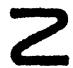
\includegraphics[keepaspectratio]{images/part002_a77d6c20.jpg}}

另一方面，当 A 是闭集时，即使 B 也是闭集，AB 也未必是闭集（参看 § 4 第 1 目命题 1 的推论 1）。

* 例如，在实直线 \(\mathbf{R}\) 的加法群中，有理整数组成的子群 \(\mathbf{Z}\) 是闭的，子群 \(\theta\mathbf{Z}\)（由全体整数倍 \(n\theta\)（\(\theta\) 为一无理数）组成）也是闭的；但子群 \(\mathbf{Z} + \theta\mathbf{Z}\)（\(\mathbf{R}\) 的），即实数 \(m + n\theta\)（其中 \(m\) 与 \(n\) 取遍一切整数值）组成的集，在 \(\mathbf{R}\) 中不是闭的，这一点我们将在第五章 § 1 中看到。

又，设 A 是 \(\mathbf{R} \times \mathbf{R}\) 的加法群中由全体点对 \((x, y)\)（满足 \(x \geqslant 0\) 与 \(0 \leqslant y \leqslant 1 - \frac{1}{x + 1}\) 的）组成的子集；并设 B 是当 x 取遍 R 时全体点对 \((x,0)\) 组成的集。A 与 B 都是闭的，但 \(A + B\) 是由全体点对 \((x,y)\)（满足 \(0 \leqslant y < 1\) 的）组成的集，它在 \(R \times R\) 中不是闭的。

设 X 是拓扑空间，f 与 g 是 X 到拓扑群 G 中的两个映射。若 f 与 g 在 X 的一点 \(x_{0}\) 处连续，则由第一章 § 2 第 1 目定理 2，\(\overline{f}^{1}\) 与 \(fg\) (*) 也连续。特别地，X 到 G 中的连续映射组成 X 到 G 的一切映射所成的群 \(\mathbf{G}^{\mathbf{x}}\) 的一个子群。

又，设 \(f\) 与 \(g\) 是集合 \(\mathbf{X}\)（由滤子 \(\mathfrak{F}\) 装备的）到 Hausdorff 拓扑群 \(\mathbf{G}\) 中的两个映射。若 \(\lim_{\mathfrak{F}} f\) 与 \(\lim_{\mathfrak{F}} g\) 存在，则 \(\lim_{\mathfrak{F}} \overline{f}^1\) 与 \(\lim_{\mathfrak{F}} fg\) 也存在，并且我们有（第一章 § 7 第 4 目命题 9 的推论 1）

\[
\lim _ {\mathfrak {F}} \overline {{f}} ^ {- 1} = (\lim _ {\mathfrak {F}} f) ^ {- 1},\tag{1}
\]

\[
\lim _ {\mathfrak {F}} f g = (\lim _ {\mathfrak {F}} f) (\lim _ {\mathfrak {F}} g).\tag{2}
\]

当 G 是写成加法形式的交换群时，公理 (GT') 表明 \((x, y) \to x - y\) 是连续映射。若 f 与 g 是拓扑空间 X 到 G 中的映射，并且在一点 \(x_{0}\) 处连续，则 f - g 在该点连续。公式 (1) 与 (2) 可以类似地改写。
% semantic-fragments: legacy-input-seam
\relax{}
\subsection{拓扑群中点的邻域}

设 \(\mathfrak{B}\) 为拓扑群 G 中单位元 \(e\) 的邻域滤子，并设 \(a\) 为 G 的任意一点。由于 \(x \to ax\) 与 \(x \to xa\) 都是同胚，因此 \(a\) 的邻域滤子是族 \(a\) . \(\mathfrak{B}\)，即由诸集合 \(a\) . V（其中 V 取遍 \(\mathfrak{B}\)）组成，它同时也是族 \(\mathfrak{B}\) . \(a\)，即由诸集合 V. \(a\) 组成。由此可见，只要知道了群的单位元 \(e\) 的邻域滤子，我们便知道了拓扑群中任意一点的邻域滤子。

如果我们说 \(xy\) 与 \(x^{-1}\) 在 \(x = y = e\) 处连续，就得到（第一章 § 2 第 1 目）：

\((\mathbf{GV}_{\mathbf{I}})\). 对任意 \(\mathbf{U} \in \mathfrak{B}\)，存在 \(\mathbf{V} \in \mathfrak{B}\) 使 \(\mathbf{V} \cdot \mathbf{V} \subset \mathbf{U}\)。

\((\mathbf{GV}_{\mathbf{II}})\). 对任意 \(\mathbf{U}\in \mathfrak{B},\) 有 \(\mathbf{U}^{-1}\in \mathfrak{B}\)

任何滤子 \(\mathfrak{B}\)，只要它在 \(G\) 上并且满足 \((\mathrm{GV}_{\mathbb{I}})\) 与 \((\mathrm{GV}_{\mathbb{II}})\)，便也满足 \((\mathrm{GV}_{\alpha})\)：对任意 \(U \in \mathfrak{B}\)，存在 \(V \in \mathfrak{B}\) 使 \(V \cdot V^{-1} \subset U\)。因为由 \((\mathrm{GV}_{\mathbb{I}})\)，存在 \(W \in \mathfrak{B}\) 使 \(W \cdot W \subset U\)；又由 \((\mathrm{GV}_{\mathbb{II}})\)，存在 \(V \in \mathfrak{B}\) 使 \(V \subset W \cap W^{-1}\)；于是 \(V^{-1} \subset W\)，从而 \(V \cdot V^{-1} \subset W \cdot W \subset U\)。

反之，设 \(\mathfrak{B}\) 为 \(\mathbf{G}\) 上满足 \((\mathrm{GV}_{\alpha})\) 的一个滤子，则首先可知 \(e\) 属于每个集合 \(\mathbf{U} \in \mathfrak{B}\)；因为若 \(\mathbf{V} \in \mathfrak{B}\) 使 \(\mathbf{V} \cdot \mathbf{V}^{-1} \subset \mathbf{U}\)，则由于 V 非空，我们有 \(x.x^{-1}=e\in U\)，它对每个 \(x\in V\) 成立。于是条件 \((\mathrm{GV}_{\alpha})\) 蕴含 \(V^{-1}\subset V.V^{-1}\subset U\)，因而 \(U^{-1}\in\mathfrak{B}\)（只要 \(U\in\mathfrak{B}\)）。最后，若 \(V\in\mathfrak{B}\) 使 \(V.V^{-1}\subset U\)，且 \(W\in\mathfrak{B}\) 使 \(W\subset V\cap V^{-1}\)，则 \(W.W\subset U\)。由此可见，\((\mathrm{GV}_{\alpha})\) 等价于 \((\mathrm{GV}_{I})\) 与 \((\mathrm{GV}_{II})\) 的合取。

最后，由于 \(x \rightarrow axa^{-1}\) 是使 e 固定不动的同胚，B 具有下列性质：

\((\mathrm{GV}_{\mathrm{III}})\). 对所有 \(a \in \mathbf{G}\) 与所有 \(\mathbf{V} \in \mathfrak{B}\)，有 \(a. \mathbf{V}.a^{-1} \in \mathfrak{B}\)。

滤子 \(\mathfrak{B}\) 的这三个性质是特征性质：

命题 1 设 G 是一个群，B 是 G 上满足公理 \((\mathrm{GV}_{\mathrm{I}})\)、\((\mathrm{GV}_{\mathrm{II}})\) 与 \((\mathrm{GV}_{\mathrm{III}})\) 的一个滤子。则在 G 上存在唯一的与 G 的群结构相容的拓扑，使 B 是单位元 e 的邻域滤子。对这个拓扑，任一点 \(a \in G\) 的邻域滤子与两个滤子 a.B 和 B.a 中的每一个都相同。

如果存在具有所需性质的拓扑，那么由上文所述，\(a\) 的邻域滤子与两个滤子 \(a\) . \(\mathfrak{B}\) 和 \(\mathfrak{B}.a\) 中的每一个都重合；因此，如果这样的拓扑存在，它便是唯一的。只要证明 1) 诸滤子 \(a\) . \(\mathfrak{B}\) 是 \(\mathbf{G}\) 上某个拓扑的邻域滤子，以及 2) 这个拓扑与 \(\mathbf{G}\) 的群结构相容，存在性便得证。

\begin{enumerate}
\def\labelenumi{\arabic{enumi})}
\item
  滤子 \(a. \mathfrak{B}\) 满足公理 \((\mathrm{V}_{\mathrm{III}})\)（见第一章 § 1 第 2 目），这由 \((\mathrm{GV}_{\mathrm{I}})\) 与 \((\mathrm{GV}_{\mathrm{II}})\) 推出，我们前面已经看到；因此，要证明 \(a. \mathfrak{B}\) 是 \(a\) 在 \(G\) 上一个拓扑中的邻域滤子，只需验证公理 \((\mathrm{V}_{\mathrm{IV}})\)。设 \(V\) 是 \(\mathfrak{B}\) 中任一集合，\(W\) 是 \(\mathfrak{B}\) 中使 \(W.W \subset V\) 的一个集合；则对任意 \(x \in a.W\)，有 \(x.W \subset a.W.W \subset a.V\)，于是 \(a.V\) 属于滤子 \(x. \mathfrak{B}\)；因而 \((\mathrm{V}_{\mathrm{IV}})\) 得到满足。
\item
  我们现在证明由邻域滤子 \(a\) . \(\mathfrak{B}\) 所定义的拓扑满足 (GT')。设 \(a, b\) 是 G 的任意两点；若令 \(x = au\)、\(y = bv\)，则我们要证明：\(xy^{-1}\) 可以随意地接近 \(ab^{-1}\)，只要 \(u\) 与 \(v\) 充分接近 \(e\)。现在 \((ab^{-1})^{-1}(xy^{-1}) = buv^{-1}b^{-1}\)；设 U 是 \(e\) 的任一邻域，则我们将有 \(buv^{-1}b^{-1} \in U\)，只要 \(uv^{-1} \in b^{-1}Ub = V\)，并且 \(V \in \mathfrak{B}\)（由 \((\mathrm{GV}_{\mathrm{III}})\)）。但由 \((\mathrm{GV}_{\mathrm{I}})\) 与 \((\mathrm{GV}_{\mathrm{II}})\)，存在 \(W \in \mathfrak{B}\) 使 \(W.W^{-1} \subset V\)；因此只需取 \(u \in W\) 与 \(v \in W\)，便有 \(xy^{-1} \in (ab^{-1})U\)。证毕。
\end{enumerate}

在 G 上定义一个与群结构相容的拓扑，一个常用方法是给出一个满足公理 \((\mathrm{GV}_{\mathrm{I}})\)、\((\mathrm{GV}_{\mathrm{II}})\) 与 \((\mathrm{GV}_{\mathrm{III}})\) 的滤子。对于滤子基 B，相应的条件如下：

\((\mathbf{GV}_{\mathbf{I}}^{\prime})\). 对任意 \(\mathbf{U}\in \mathfrak{B}\)，存在 \(\mathbf{V}\in \mathfrak{B}\) 使 \(\mathbf{V}.\mathbf{V}\subset \mathbf{U}\)。\((\mathrm{GV}_{\mathrm{II}}^{\prime})\). 对任意 \(\mathbf{U} \in \mathfrak{B}\)，存在 \(\mathbf{V} \in \mathfrak{B}\) 使 \(\mathbf{V}^{-1} \subset \mathbf{U}\)。\((\mathrm{GV}_{\mathrm{III}}^{\prime})\). 对任意 \(a \in \mathbf{G}\) 与任意 \(\mathbf{U} \in \mathfrak{B}\)，存在 \(\mathbf{V} \in \mathfrak{B}\) 使 \(\mathbf{V} \subset a. \mathbf{U}. a^{-1}\)。

e 的一个邻域若与它在对称映射 \(x \rightarrow x^{-1}\) 下的像重合，就称为对称邻域。若 V 是 e 的任一邻域，则 \(V \cup V^{-1}\)、\(V \cap V^{-1}\) 与 \(V \cdot V^{-1}\) 都是对称邻域。由 \((\mathrm{GV}_{\mathrm{II}})\)，诸对称邻域构成 e 的一个基本邻域系。又由 \((\mathrm{GV}_{\mathrm{I}})\)，当 V 取遍 e 的一个基本邻域系时，诸集合 \(V^{n}\)（其中 n 是一个固定的整数 \(\neq 0\)）构成 e 的一个基本邻域系。

注。若 G 是交换群，则有 \(x \cdot A \cdot x^{-1} = A\)（对 G 的每个子集 A 及每个 \(x \in G\)），因而 \((GV_{III})\){[}相应地 \((GV_{III}')\){]}对 G 上每个滤子（相应地，滤子基）自动满足。另一方面，若 G 不是交换群，则 \((GV_{III})\) 不是 \((GV_I)\) 与 \((GV_{II})\) 的推论{[}参看习题 5{]}。

若 G 是以加法记写的交换群，则刻画与 G 的群结构相容的拓扑的原点邻域滤子 B 的公理就是下列两条：\((\mathrm{GA}_{\mathrm{I}})\). 对任意 \(U \in B\)，存在 \(V \in B\) 使 \(V + V \subset U\)。\((\mathrm{GA}_{\mathrm{II}})\). 对任意 \(U \in B\)，有 \(-U \in B\)。

命题 2 拓扑群 G 是 Hausdorff 群，当且仅当集合 \(\{e\}\) 是闭集。

显然，若 G 是 Hausdorff 群，则 \(\{e\}\) 是闭集。反之，若 \(\{e\}\) 是闭集，则对角线 \(\Delta\)（\(G \times G\) 的）是闭集，因为它是 \(\{e\}\) 在连续映射 \((x, y) \to xy^{-1}\) 下的逆像；于是（第一章 § 8 第 1 目命题 1）G 是 Hausdorff 群。

推论 拓扑群 G 是 Hausdorff 群，当且仅当 e 的诸邻域之交仅由点 e 组成。

该条件显然必要。反之，若 \(e\) 的所有邻域之交恰为 \(\{e\}\)，则对任意 \(x \neq e\)，存在一个邻域 \(V\)（\(e\) 的），使 \(x^{-1} \notin V\)，因而 \(e \notin xV\)。这表明 \(x\) 不属于 \(\{e\}\) 的闭包，从而 \(\{e\}\) 是闭集，于是 \(G\) 是 Hausdorff 群。

例。借助一组子群来定义群上的拓扑。设 \(\mathfrak{B}\) 是群 \(\mathbf{G}\) 上由 \(\mathbf{G}\) 的子群组成的一个滤子基，则直接可以看出 \(\mathfrak{B}\) 满足公理 \((\mathrm{GV}_{\mathrm{I}}^{\prime})\) 与 \((\mathrm{GV}_{\mathrm{II}}^{\prime})\)，因为 \(\mathbf{H}.\mathbf{H}^{-1} = \mathbf{H}\)，其中 \(\mathbf{H}\) 是 \(\mathbf{G}\) 的任一子群。因此，集合 \(\mathfrak{B}\) 将是 \(e\) 在某个与 \(\mathbf{G}\) 的群结构相容的拓扑中的基本邻域系，只要 \(\mathfrak{B}\) 满足 \((\mathrm{GV}_{\mathrm{III}})\)；特别地，当 \(\mathfrak{B}\) 中所有子群都是正规子群时即属此情形，因而在 \(G\) 是交换群时永远如此。这样定义的拓扑，按命题 2，是 Hausdorff 的当且仅当 \(\mathfrak{B}\) 中所有子群之交仅由 \(e\) 组成。最有意义的情形是子群 \(\{e\}\) 不属于 \(\mathfrak{B}\) 的情形（否则由 \(\mathfrak{B}\) 定义的拓扑是离散拓扑）：若 \(\{e\} \notin \mathfrak{B}\)，则由 \(\mathfrak{B}\) 定义的拓扑只有在 \(\mathfrak{B}\) 是无限集时才可能是 Hausdorff 的。

由于两个子群之交是子群，我们可以从 G 的任意一组子群 \(\mathfrak{F}\) 出发，在 G 上定义一个与其群结构相容的拓扑：设 \(\mathfrak{G}\) 是所有形如 \(a.H.a^{-1}\) 的子群组成的集，其中 \(H\in\mathfrak{F}\) 且 \(a\in G\)；再设 \(\mathfrak{B}\) 是属于 \(\mathfrak{G}\) 的子群的所有有限交组成的集。则 \(\mathfrak{B}\) 是一个滤子基且满足 \((\mathrm{GV}_{\mathrm{III}}^{\prime})\)。

特别地，考虑环 A 的加法群。A 的理想的任意一个集合 \(\mathfrak{F}\) 都定义一个与这个加法群结构相容的拓扑。若 \(\mathfrak{F}\) 中所有理想之交是零理想，则这个拓扑是 Hausdorff 的；若 \(\mathfrak{F}\) 中诸理想的任何有限交都不是零理想，则它不是离散的。用这种方式定义的拓扑在数论中起很大作用（见本章 § 6 与 § 7 的习题）。

\subsection{同构与局部同构}

按照一般定义（《集合论》，第四章，§ 1，第 5 目），同构 \(f\)（拓扑群 \(G\) 到拓扑群 \(G'\) 上的）指的是 \(G\) 到 \(G'\) 上的一个双射，它既是 \(G\) 的群结构到 \(G'\) 的群结构上的一个同构，又是 \(G\) 到 \(G'\) 上的一个同胚。换言之，\(f\) 是 \(G\) 到 \(G'\) 上的同构，当且仅当：1) \(f\) 是双射；2) \(f(xy) = f(x)f(y)\) 对所有 \(x, y \in G\) 成立；3) \(f\) 是双连续的。

例如，若 \(a\) 是 \(G\) 的任一点，则映射 \(x \to axa^{-1}\) 是 \(G\) 到 \(G\) 上的一个同构，即（同处所引）拓扑群 \(G\) 的一个自同构。它称为内自同构。

若拓扑 \(\mathfrak{C}\) 与群 \(\mathbf{G}\) 的群结构相容，则 \(\mathfrak{C}\) 也与 \(\mathbf{G}\) 的反群结构相容。若以 \(\mathbf{G}^0\) 表示把 \(\mathbf{G}\) 的反群赋予拓扑 \(\mathfrak{C}\) 所得的拓扑群，则对称映射 \(x \to x^{-1}\) 是拓扑群 \(\mathbf{G}\) 到拓扑群 \(\mathbf{G}^0\) 上的一个同构。

定义 2 若 G 与 G' 是两个拓扑群，则 G 与 G' 的局部同构指的是 G 的单位元的邻域 V 到 G' 的单位元的邻域 V' 上的一个同胚 f，它满足下列条件：

\begin{enumerate}
\def\labelenumi{\arabic{enumi})}
\tightlist
\item
  对每对点 \(x, y\)（属于 \(V\) 且使 \(xy \in V\)），
\end{enumerate}

\[
f (x y) = f (x) f (y).
\]

\begin{enumerate}
\def\labelenumi{\arabic{enumi})}
\setcounter{enumi}{1}
\tightlist
\item
  若 \(g\) 是 \(f\) 的逆映射，则对每对点 \(x', y'\)（属于 \(V'\) 且使 \(x'y' \in V'\)），有 \(g(x'y') = g(x')g(y')\)。
\end{enumerate}

这时映射 g 是 \(G'\) 与 G 的一个局部同构。

两个拓扑群 G、G' 称为局部同构的，如果存在 G 与 G' 的一个局部同构。

同构的拓扑群显然是局部同构的。反之不成立。

* 例如，我们将在第五章 § 1 中看到，拓扑群 R 与 T 局部同构但不同构。*

若 \(f\) 是 \(G\) 与 \(G'\) 的一个局部同构，则 \(f\) 到 \(G\) 的单位元的一个邻域上的每个限制仍是 \(G\) 与 \(G'\) 的局部同构。

G 与 G 的局部同构称为 G 的局部自同构。

一般地，若 \(f\) 是邻域 \(V\)（\(G\) 的单位元的）到邻域 \(V'\)（\(G'\) 的单位元的）上的一个同胚，且满足定义 2 的条件 1)，则 \(f\) 未必满足条件 2)（见习题 7）。尽管如此，\(G\) 与 \(G'\) 实际上是局部同构的。

命题 3 设 G 与 G' 是两个拓扑群，f 是 G 的单位元的邻域 V 到 G' 的单位元的邻域 V' 上的一个同胚，且满足定义 2 的条件 1)。则 f 是 G 与 G' 的一个局部同构的延拓。

因为不难看出，若 W 是 G 的单位元的一个使 \(W.W \subset V\) 的邻域，则 f 到 W 上的限制是 G 与 \(G'\) 的一个局部同构。

\section{子群、商群、同态、齐性空间、积群}

\subsection{拓扑群的子群}

设 G 是一个拓扑群，H 是 G 的一个子群。由 (GT')，G 的拓扑在 H 上诱导的拓扑与 H 的群结构相容。这样在 H 上定义的拓扑群结构称为由 G 的结构诱导的结构。每当我们把 G 的子群 H 当作拓扑群考虑时，除另有明确说明外，所指的总是这个诱导结构。

命题 1 拓扑群 G 的子群 H 的闭包 \(\overline{H}\) 是 G 的一个子群。若 H 是 G 的正规子群，则 \(\overline{H}\) 也是。

若 \(a, b \in \overline{\mathbf{H}}\)，则 \(ab^{-1} \in \overline{\mathbf{H}}\)，因为映射 \((x, y) \to xy^{-1}\) 在 \(\mathbf{G} \times \mathbf{G}\) 上连续且把 \(\mathbf{H} \times \mathbf{H}\) 变换为 \(\mathbf{H}\)（第一章 § 2 第 1 目定理 1）。同样，映射 \(x \to axa^{-1}\) 的连续性表明：若 \(\mathbf{H}\) 是正规子群，则 \(\overline{\mathbf{H}}\) 是正规子群。

特别地，仅由 G 的单位元组成的集合 \(\{e\}\) 的闭包 N 是 G 的一个正规子群；且 \(N=\{e\}\) 当且仅当 G 是 Hausdorff 群（§ 1 第 2 目命题 2）。

命题 2 若 G 是 Hausdorff 拓扑群，则 G 的交换子群的闭包是 G 的交换子群。

由于命题 1，我们可以局限于 H 在 G 中稠密的情形。连续函数 xy 与 yx 在 H × H 上相等，因而由恒等延拓原理（第一章 § 8 第 1 目命题 2 推论 1），它们在 G × G 上相等。

命题 3 设 G 是 Hausdorff 拓扑群，M 是 G 的任一子集。则 G 中与 M 的每个元素交换的元素组成的集 M' 是 G 的一个闭子群。特别地，G 的中心在 G 中是闭的。

因为 \(\mathbf{M}'\) 是诸集合 \(\mathbf{F}_m(m \in \mathbf{M})\) 之交，其中 \(\mathbf{F}_m\) 是所有这样的 \(x \in \mathbf{G}\) 组成的集，它们使 \(xm = mx\)；而 \(\mathbf{F}_m\) 是闭的（第一章 § 8 第 1 目命题 2）。

命题 4 设 G 是一个拓扑群，H 是 G 的一个子群，它在 H 的某一点处是局部闭的（第一章 § 3 第 3 目定义 2）。则 H 在 G 中是闭的。

由平移，H 在其每一点处都是局部闭的，即 H 在 G 中是局部闭的。设 V 是 e 在 G 中的一个对称开邻域，使 \(V \cap H\) 在 V 中是闭的。若 \(x \in \overline{H}\)，则 xV 与 H 相交；若 \(y \in xV \cap H\)，则有 \(x \in yV\)，且 \(y(V \cap H) = (yV) \cap H\) 在 yV 中是闭的。但 x 属于 \((yV) \cap H\) 的闭包，故 \(x \in H\)。

推论 拓扑群的子群是开的，当且仅当它有一个内点。每个开子群都是闭的。

若子群 H 有一个内点，则由平移，H 的所有点都是内点，因而 H 是开的。推论的第二个断言是命题 4 的一个特殊情形。

命题 5 拓扑群 G 的子群 H 是离散的，当且仅当 H 有一个孤立点。Hausdorff 群的每个离散子群都是闭的。

若 H 是离散的，则 H 的每一点都是孤立点。反之，若 H 有一个孤立点，则由平移，H 的每一点都是孤立点，因此 H 是离散的。若 H 离散且 G 是 Hausdorff 群，则存在 e 的一个邻域 V 使 \(V \cap H = \{e\}\)；\(\{e\}\) 在 G 中是闭的，因而在 V 中更加是闭的，于是 H 在 e 处是局部闭的。故由命题 4，H 在 G 中是闭的。

注。设 H 是拓扑群 G 的任一子群。对每个 \(x \in \overline{H}\)，有 \(\overline{xH} = x\) . \(\overline{H} = \overline{H}\)，因为 x 平移是 G 到 G 上的同胚。换言之，对每个 \(x \in \overline{H}\)，xH 在 \(\overline{H}\) 中稠密。由此可得，若 H 不是闭的，则 \(\overline{H} \cap \mathrm{C}H\) 在 \(\overline{H}\) 中稠密。

\subsection{拓扑群的连通分支}

设 V 是 e 在 G 中的一个对称邻域。由 V 生成的子群记作 \(V^{\infty}\)，它由 V 中元素的有限序列的所有乘积 \(\prod_{i=1}^{n} x_{i}\) 组成。\(V^{\infty}\) 是开的，因为它以 e 为一个内点，因而由第 1 目命题 4 是闭的。由此可得：

命题 6 连通拓扑群由单位元的每个邻域生成。

正如我们将在第四章（§ 2 第 5 目）看到的，这个命题的逆命题一般不成立。若拓扑群 G 由单位元的每个邻域生成，我们至多能说 G 除 G 外不含任何开子群。

* 作为具有异于 G 的开子群的非连通群 G 的例子，可以举出非零实数的乘法群 \(\mathbf{R}^{*}\)，其中子群 \(\mathbf{R}_{+}^{*}\)（由实数 \textgreater0 组成的）既开又闭（见第四章 § 3 第 2 目）。*

命题 7 在拓扑群 G 中，单位元 e 的连通分支 K 是一个闭正规子群。任一点 \(x \in G\) 的连通分支是陪集 \(x.K = K.x\)。

若 \(a \in \mathbf{K}\)，则 \(a^{-1}\mathbf{K}\) 连通且包含 \(e\)；于是 \(\mathbf{K}^{-1}\mathbf{K} \subset \mathbf{K}\)，这表明 \(\mathbf{K}\) 是 \(\mathbf{G}\) 的一个子群。这个子群在 \(\mathbf{G}\) 的所有自同构下不变，特别在所有内自同构下不变，因此 \(\mathbf{K}\) 在 \(\mathbf{G}\) 中是正规的；又 \(\mathbf{K}\) 是闭的（第一章 § 11 第 5 目命题 9）。最后，左平移 \(y \to xy\) 是 \(\mathbf{G}\) 的一个把 \(e\) 映为 \(x\) 的同胚，因而 \(x\) 的连通分支是 \(x\cdot \mathbf{K}\)。

G 的单位元 e 的连通分支称为 G 的单位元连通分支。

\subsection{稠密子群}

下面的命题推广了第 1 目的命题 1：

命题 8 设 H 是拓扑群 G 的一个稠密子群，K 是 H 的一个正规子群。则 K 在 G 中的闭包 \(\overline{K}\) 是 G 的一个正规子群。

因为映射 \((z, x) \to zxz^{-1}\) 在 \(\mathbf{G} \times \mathbf{G}\) 上连续，且把 \(\mathbf{H} \times \overline{\mathbf{K}}\) 映入 \(\overline{\mathbf{K}}\)；所以（第一章 § 2 第 1 目定理 1）它把 \(\mathbf{G} \times \overline{\mathbf{K}} = \overline{\mathbf{H}} \times \overline{\mathbf{K}}\) 映入 \(\overline{\mathbf{K}}\)。

命题 9 设 H 是拓扑群 G 的一个稠密子群。若 H 由 H 中单位元的每个邻域生成，则 G 由 G 中单位元的每个邻域生成。

设 V 是 e 在 G 中的任一对称邻域。则 \(V \cap H\) 是 e 在 H 中的一个邻域，因而生成 H。由此可知 V 生成一个包含 H 的子群 \(H'\)；而 \(H'\) 是既开又闭的（第 1 目命题 4 的推论），因此包含 \(\overline{H} = G\)。

\subsection{带算子空间}

设 X 是一个拓扑空间，G 是一个拓扑群。如果下列条件得到满足，就称 G 连续作用在 X 上：

\begin{enumerate}
\def\labelenumi{\arabic{enumi})}
\item
  X 以 G 为算子群；换言之，X 赋有一个外合成法则 \((s, x) \to s.x\)，G 是它的算子集，并且 \(s.(t.x) = (st).x\) 与 e.x = x 对所有 \(s, t \in G\) 与所有 \(x \in X\) 成立。
\item
  映射 \((s, x) \to s.x\)（从 \(\mathbf{G} \times \mathbf{X}\) 到 \(\mathbf{X}\) 中的）是连续的。
\end{enumerate}

引理 1 若拓扑群 G 连续作用在拓扑空间 X 上，则对每个 \(s \in \mathbf{G}\)，映射 \(x \to s.x\) 是 X 到 X 上的一个同胚。

因为这个映射是一个连续双射，其逆 \(x \rightarrow s^{-1}.x\) 也是连续的。

我们回顾，对每个 \(x \in X\)，x 在 G 的元素 s 下的变换 s.x 组成的集 G.x 称为 x 的轨道（关于算子群 G 的），而使 s.x = x 的所有 \(s \in G\) 组成的集是 G 的一个子群，称为 x 的稳定子群。关系 \(\mathrm{R}(x, y) : ``y \text{ 属于轨道 } x''\) 是 X 上的一个等价关系，称为由 G 定义的等价关系；关于这个关系的诸等价类就是 X 的诸点的轨道。拓扑空间 X/R 称为 X 的轨道空间（关于 G 的），或 X 关于群 G 的商空间，记作 X/G；并称 X/G 的拓扑为 X 的拓扑经 G 的商。

引理 2 若拓扑群 G 连续作用在拓扑空间 X 上，则由 G 定义的等价关系 R 是开的。

因为关于 \(\mathbf{R}\) 取的 \(\mathbf{U}\)（\(\mathbf{X}\) 的一个开子集）的饱和集是集合 \(\bigcup_{s\in G}s.\mathbf{U},\)，而由引理 1，每个 \(s.\mathbf{U}\) 都是开的。

例。1) 设 H 是拓扑群 G 的一个子群。H 通过外法则 \((s, x) \rightarrow sx\) 连续作用在 G 上。H 也通过外法则 \((x, s) \rightarrow sxs^{-1}\) 连续作用在 G 上。

\begin{enumerate}
\def\labelenumi{\arabic{enumi})}
\setcounter{enumi}{1}
\item
  *若 K 是一个拓扑除环（§ 6 第 7 目），则乘法群 K* 通过外法则 \((s, x) \to sx\) 连续作用在 K 上。*
\item
  设 G 是一个拓扑群，X 是一个拓扑空间。则映射 \((s, x) \to x\)（从 \(G \times X\) 到 X 中的）是 X 上的一个外合成法则，且 G 关于这个法则连续作用在 X 上；这时称 G 平凡地作用在 X 上。
\end{enumerate}

注。与其说拓扑群 G 连续作用在拓扑空间 X 上，人们常说 G 在 X 的左边连续作用。当 G 的反群 \(G^{0}\)（拓扑群）连续作用在 X 上时，我们说 G 在 X 的右边连续作用。这等同于说：X 有一个连续的外合成法则 \((s, x) \to s.x\)，以 G 为算子集，满足 \(s.(t.x) = (ts).x\) 与 e.x = x。这样的法则常写在右边：\((s, x) \to x.s\)（术语即由此而来），这时有 \((x.t).s = x.(ts)\)。若 G 通过法则 \((s, x) \to x.s\) 在 X 上右边连续作用，则 G 也依照外法则 \((s, x) \to x.s^{-1}\) 在 X 上左边连续作用，这是由公理 \((\mathrm{GT}_{\mathrm{II}})\) 得出的。

设 X（相应地，X'）是带算子群 G（相应地，G'）的集合，\(f: \mathbf{G} \to \mathbf{G}'\) 是一个同态，\(g: \mathbf{X} \to \mathbf{X}'\) 是一个映射。则称 \(f\) 与 \(g\) 是相容的，如果 \(g(s.x) = f(s).g(x)\) 对所有 \(s \in \mathbf{G}\) 与所有 \(x \in \mathbf{X}\) 成立。若 \(\mathbf{X}''\) 是第三个带算子群 G'' 的集合，\(f': \mathbf{G}' \to \mathbf{G}''\) 是一个同态，\(g': \mathbf{X}' \to \mathbf{X}''\) 是一个映射，且 \(f'\) 与 \(g'\) 相容，则 \(f' \circ f\) 与 \(g' \circ g\) 相容。当 X、X' 是拓扑空间且 G、G' 是分别连续作用在 X、X' 上的拓扑群时，就称 \((f, g)\) 为带算子空间 X 到带算子空间 X' 中的态射，只要 \(f\) 与 \(g\) 是连续且相容的。过渡到商，\(g\) 便诱导出连续映射 \(\mathbf{X}/\mathbf{G} \to \mathbf{X}'/\mathbf{G}'\)（第一章 § 3 第 4 目命题 6 的推论）。

设 G 是连续作用在拓扑空间 X 上的一个拓扑群，\(\varphi\) 是 X 到轨道空间 X/G 上的典范映射。设 A 是 X 的任一子集，\(A'\) 是 X 中作为 A 关于由 G 定义的等价关系 R 的饱和集的子空间（于是 \(A'\) 是 A 的诸点的轨道之并，称为 A 关于 G 的饱和集）。G 连续作用在 \(A'\) 上，其作用法则是 \((s, x) \to s.x\) 到 \(G \times A'\) 上的限制。此外，由于 R 是开的（引理 2）且 \(A'\) 是饱和的，由第一章 § 5 第 2 目命题 4 以及关系式 \(\varphi(A) = \varphi(A')\) 可得：

命题 10 子空间 \(\varphi(A)\)（\(X/G\) 的）到轨道空间 \(A'/G\) 上的典范双射是一个同胚。

现设 S 是 X 上的一个等价关系，使得对每个 \(s \in G\)，映射 \(x \to s.x\) 与 S 相容{[}换言之，使得关系 \(x \equiv y \pmod{S}\) 蕴含 \(s.x \equiv s.y \pmod{S}\){]}；为简便起见，我们将说关系 S 与群 G 相容。若 \(\psi\) 是 X 到 X/S 上的典范映射，且以 \(s.\psi(x)\) 表示 s.x 的模 S 类，则 X/S 关于外法则 \((s, \psi(x)) \to s.\psi(x) = \psi(s.x)\) 以 G 为算子群。此外：

命题 11 若 X 上的等价关系 S 是开的且与 G 相容，则 G 连续作用在 X/S 上。

由于 G 上的相等关系与 X 上的关系 S 都是开的，只需证明映射 \((s,x)\to s.\psi(x)=\psi(s.x)\)（从 \(G\times X\) 到 X/S 中的）是连续的（第一章 § 5 第 3 目命题 8 的推论）；而这由 \(\psi\) 的连续性以及映射

\[
(s, x) \rightarrow s. x.
\]

注。设 \(G'\) 是另一个连续作用在 X 上的拓扑群，并设 \(s.(s'x) = s'(s.x)\) 对所有 \(s \in G\)、\(s' \in G'\) 与 \(x \in X\) 成立。则等价关系 \(S\)（由 \(G'\) 定义的）与 \(G\) 相容，且由于 \(S\) 是开的（引理 2），可知 \(G\) 连续作用在 \(X/G'\) 上。类似地，\(G'\) 连续作用在 \(X/G\) 上。在这些情形下，我们说两个群 \(G\) 与 \(G'\) 在 \(X\) 上的两个作用可交换。

\subsection{齐性空间}

设 G 是一个拓扑群，H 是 G 的一个子群。H 依照外法则 \((t, x) \to xt\) 在 G 的右边连续作用，且点 \(x \in G\) 的轨道是左陪集 xH。因此诸轨道组成的集就是我们在代数中所谓的齐性空间 G/H。每当我们把 G/H 作为拓扑空间谈论时，除相反的情况有明确说明外，所指的总是 G 的轨道空间（关于 H 的）；即 G 关于等价关系 \(x^{-1}y \in H\) 的商空间。按照一般定义，我们说这个空间的拓扑是 G 的拓扑经 H 的商。

命题 12 群 G 在每个齐性空间 G/H 上连续作用。

由于等价关系 \(x^{-1}y \in H\) 是开的（第 4 目引理 2），这是第 4 目命题 11 的一个特殊情形。

命题 13 设 G 是一个拓扑群，H 是 G 的一个子群。则齐性空间 G/H 是 Hausdorff 的，当且仅当 H 在 G 中是闭的。

H 是关系 \(x^{-1}y \in H\) 的一个等价类，因此若 G/H 是 Hausdorff 的，则 H 在 G 中是闭的。反之，若 H 是闭的，则这个关系的图在 \(G \times G\) 中是闭的，因为它是 H 在连续映射 \((x, y) \to x^{-1}y\) 下的原像。由于关系 \(x^{-1}y \in H\) 是开的，由第一章 § 8 第 3 目命题 8 可知 G/H 是 Hausdorff 的。

命题 14 设 G 是一个拓扑群，H 是 G 的一个子群。则齐性空间 G/H 是离散的，当且仅当 H 在 G 中是开的。

因为在典范映射下 G/H 的诸点在 G 中的原像是诸陪集 xH（x ∈ G）；而这些集合在 G 中是开的，当且仅当 H 在 G 中是开的。

设 X 是一个拓扑空间，拓扑群 G 连续且可迁地作用在它上面；这时 X（在代数意义上）是 G 的一个齐性空间。设 \(x\) 是 \(X\) 的一点，\(H_x\) 是它的稳定子群。连续满射 \(s \to s.x\)（\(G\) 到 \(X\) 上的）典范地分解为

\[
\mathbf {G} \xrightarrow {f _ {x}} \mathbf {G} / \mathbf {H} _ {x} \xrightarrow {g _ {x}} \mathbf {X}
\]

\pandocbounded{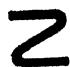
\includegraphics[keepaspectratio]{images/part002_c9cfa224.jpg}}

其中 \(f_x\) 是 \(G\) 到齐性空间 \(G/H_x\) 上的典范映射，\(g_x\) 是双射 \(s.H_x \to s.x\)（\(G/H_x\) 到 \(X\) 上的）；此外（第一章 § 3 第 4 目命题 6），\(g_x\) 是连续映射。但 \(g_x\) 未必是 \(G/H_x\) 到 \(X\) 上的一个同胚（习题 29）。若 \(g_x\) 对每个 \(x \in X\) 都是同胚，则称 \(X\)（拓扑群 \(G\) 的）为拓扑齐性空间；为此的充要条件是：对每个 \(x \in E\)，映射 \(s \to s.x\)（\(G\) 到 \(X\) 中的）是开的。

命题 15 设 X 是一个拓扑空间，拓扑群 G 连续且可迁地作用在它上面。为使 X 是（关于 G 的）拓扑齐性空间，只需对某一点 \(x_{0} \in X\)，映射 \(s \to s \cdot x_{0}\) 把 e 在 G 中的每个邻域变换为 \(x_{0}\) 在 X 中的一个邻域。

每个 \(x \in X\) 都可写作 \(x = t.x_0\)（对某个 \(t \in G\)）。若 \(V\) 是 \(e\) 的一个邻域，则 \(V.x = (Vt).x_0\) 是 \(x\) 的一个邻域，因为可以写 \((Vt).x_0 = t((t^{-1}Vt).x_0)\)，而断言由下列事实得出：\(t^{-1}Vt\) 是 \(e\) 在 \(G\) 中的一个邻域，且 \(y \to t.y\) 是 \(X\) 到其自身的一个同胚（第 4 目引理 1）。由此可得，若 \(U\) 是 \(G\) 的任一开子集且 \(x\) 是 \(X\) 的任一点，则 \(U.x\) 在 \(X\) 中是开的；因为若 \(t \in U\)，则 \(t^{-1}U\) 是 \(e\) 的一个邻域，因而 \((t^{-1}U).x\) 是 \(x\) 的一个邻域，且 \(t.((t^{-1}U).x) = U.x\) 是 \(t.x\) 的一个邻域。于是 \(U.x\) 在 \(X\) 中是开的，从而映射 \(s \to s.x\)（\(G\) 到 \(X\) 中的）是开的。证毕。

\subsection{商群}

命题 16 设 G 是一个拓扑群，H 是 G 的一个正规子群。则 G 的拓扑经 H 的商与 G/H 的群结构相容。

若 \(x \to \dot{x}\) 是 G 到 G/H 上的典范映射，则我们要证明的是：\((\dot{x}, \dot{y}) \to \dot{x}\dot{y}^{-1}\) 是 (G/H) \(\times\) (G/H) 到 G/H 中的一个连续映射。由于等价关系 \(x^{-1}y \in H\) 是开的（第 4 目引理 2），只需证明 \((x,y) \to \dot{x}\dot{y}^{-1}\) 是 G \(\times\) G 到 G/H 中的一个连续映射（第一章 § 5 第 3 目命题 8 的推论，以及 § 3 第 4 目命题 6）。但 \((x,y) \to \dot{x}\dot{y}^{-1}\) 是连续映射 \(x \to \dot{x}\) 与 \((x,y) \to xy^{-1}\) 的复合，因而是连续的。

在后续内容中，每当我们把拓扑群 G 的商群 G/H 作为拓扑群考虑时，除相反的情况有明确说明外，总应理解为 G/H 的拓扑是 G 的拓扑经 H 的商。

命题 17 设 \(\varphi\) 是拓扑群 \(\mathbf{G}\) 到商群 \(\mathrm{G / H}\) 上的典范映射。若 \(\mathfrak{B}\) 是 \(e\) 在 \(\mathbf{G}\) 中的一个基本邻域系，则 \(\varphi(\mathfrak{B})\) 是单位元 \(\varphi(e)\)（\(\mathrm{G / H}\) 的）的一个基本邻域系。

这是第一章 § 5 第 3 目命题 5 的一个特殊情形。

命题 13 与 14 对商群特别地给出：

命题 18 设 G 是一个拓扑群，H 是 G 的一个正规子群。

\begin{enumerate}
\def\labelenumi{\alph{enumi})}
\item
  商群 G/H 是 Hausdorff 的，当且仅当 H 在 G 中是闭的。
\item
  商群 G/H 是离散的，当且仅当 H 在 G 中是开的。
\end{enumerate}

若 G 是一个拓扑群，N 是 \(\{e\}\) 在 G 中的闭包，则 N 是 G 的一个闭正规子群（第 1 目命题 1），因而 G/N 是 Hausdorff 的；G/N 称为 G 的伴随 Hausdorff 群。

命题 19 若 H 是拓扑群 G 的一个离散正规子群，则 G/H 与 G 局部同构。

设 \(\mathbf{V}\) 是 \(e\) 在 \(\mathbf{G}\) 中的一个邻域，它不含 \(\mathbf{H}\) 中除 \(e\) 外的任何点，又设 \(\mathbf{W}\) 是 \(e\) 在 \(\mathbf{G}\) 中的一个对称开邻域，使得 \(\mathbf{W}^2 \subset \mathbf{V}\)。则 \(\mathbf{W}\) 上典范映射 \(\varphi\)（\(\mathbf{G}\) 到 \(\mathbf{G} / \mathbf{H}\) 上的）的限制是单射；因为若 \(x, y \in \mathbf{W}\) 且 \(\varphi(x) = \varphi(y)\)，则 \(x^{-1}y \in \mathbf{W}^2 \subset \mathbf{V}\) 且 \(x^{-1}y \in \mathbf{H}\)，于是 \(x = y\)。由命题 17 可知 \(\varphi\) 在 \(\mathbf{W}\) 上的限制是 \(\mathbf{W}\) 到 \(\varphi(\mathbf{W})\) 上的一个同胚；又因 \(\varphi(xy) = \varphi(x)\varphi(y)\) 对所有 \(x, y \in \mathbf{W}\) 成立，我们断定 \(\mathbf{G}\) 与 \(\mathbf{G} / \mathbf{H}\) 局部同构（§ 1 第 3 目命题 3）。

\subsection{商群的子群与商群}

设 G 是一个拓扑群，H 是 G 的一个正规子群，\(\varphi: G \to G/H\) 是典范映射。我们知道，若 \(A'\) 是 G/H 的一个子群，则 \(\varphi^{-1}(A')\) 是 G 的一个包含 H 的子群。反之，若 A 是 G 的一个子群，则 \(\varphi(A)\) 是 G/H 的一个子群；此外，存在商群 \(A/(A \cap H)\) 到 G/H 的子群 \(\varphi(A)\) 上的一个典范双射，以及 \(\varphi(A)\) 到商群 AH/H 上的一个典范双射，且这两个双射对群结构而言都是同构。

命题 20 设 A 是拓扑群 G 的一个子群，H 是 G 的一个正规子群，\(\varphi\) 表示 G 到 G/H 上的典范映射。则 \(\varphi(A)\) 到 AH/H 上的典范双射是拓扑群的一个同构。

这由前面的注记以及第 4 目命题 10 得出。

\pandocbounded{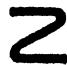
\includegraphics[keepaspectratio]{images/part002_0097f9c2.jpg}}

\(\mathbf{A}/(\mathbf{A} \cap \mathbf{H})\) 到 \(\varphi(\mathbf{A})\) 上的典范双射是连续同态，因为它是由 \(\varphi\) 在 \(\mathbf{A}\) 上的限制过渡到商而产生的；但一般地说，拓扑群 \(\mathbf{A}/(\mathbf{A} \cap \mathbf{H})\) 与 \(\mathbf{AH}/\mathbf{H}\) 不同构（参看 § 4 第 1 目命题 1 推论 3）。

* 例如，取 G 为实数的加法群 R，取 H 为整数群 Z，取 A 为一个无理数 θ 的整数倍组成的群 θZ。则 A∩H = \{0\}，因而 A/(A∩H) 是一个离散群，同构于 Z；另一方面，A + H 在 R 中稠密（我们将在第五章 § 1 第 1 目命题 1 中看到），于是 (A + H)/H——它与 A + H 局部同构（第 6 目命题 19）——不是离散群，从而不同构于 A/(A∩H)。*

尽管如此，我们有下面的命题：

命题 21 设 G 是一个拓扑群，\(G_{0}\) 是 G 的一个稠密子群，\(H_{0}\) 是 \(G_{0}\) 的一个正规子群，H 是 \(H_{0}\) 在 G 中的闭包，\(\varphi\) 是典范映射 \(G \rightarrow G/H\)。则典范双射 \(G_{0}/H_{0} \rightarrow \varphi(G_{0})\) 是拓扑群 \(G_{0}/H_{0}\) 到 G/H 的一个稠密子群上的一个同构。

由于 \(\mathbf{H}_0 = \mathbf{H} \cap \mathbf{G}_0\)，只需证明：若 \(\mathbf{U}_0\) 是 \(\mathbf{G}_0\) 的任一开子集，它关于关系 \(x^{-1}y \in \mathbf{H}_0\) 是饱和的，则 \(\mathbf{U}_0\) 是 \(\mathbf{G}_0\) 与 \(\mathbf{G}\) 的一个关于关系 \(x^{-1}y \in \mathbf{H}\) 饱和的开子集的交（第一章 § 3 第 6 目命题 10）。设 \(\mathbf{U}\) 是 \(\mathbf{G}\) 的一个使 \(\mathbf{U}_0 = \mathbf{U} \cap \mathbf{G}_0\) 的开子集。由于 \(\mathbf{U}_0 = \mathbf{U}_0\mathbf{H}_0\)，容易看出 \(\mathbf{U}_0 = \mathrm{UH}_0 \cap \mathbf{G}_0\)；但 \(\mathrm{UH}_0\) 在 \(\mathbf{G}\) 中是开的，故可设 \(\mathbf{U} = \mathrm{UH}_0\)。集合 \(\mathrm{UH}\) 在 \(\mathbf{G}\) 中是开的且关于关系 \(x^{-1}y \in \mathbf{H}\) 是饱和的；因此只要证明 \(\mathrm{UH} \cap \mathbf{G}_0 = \mathbf{U}_0\)，命题就证明了。现在，若 \(u \in \mathbf{U}\) 与 \(h \in \mathbf{H}\) 使 \(uh \in \mathbf{G}_0\)，则存在一个对称邻域 \(\mathbf{V}\)（\(e\) 在 \(\mathbf{G}\) 中的），使得 \(uv \subset U\)；由于 \(Vh\) 是 \(h\) 在 \(\mathbf{G}\) 中的一个邻域，存在 \(z \in V\) 使 \(zh \in \mathbf{H}_0\)。于是有 \(uz^{-1} \in U\)，且 \(uh = (uz^{-1})(zh)\)；因此 \(\mathrm{UH} \cap \mathbf{G}_0 \subset \mathrm{UH}_0\)。但 \(\mathrm{UH}_0 = U\)，于是 \(\mathrm{UH} \cap \mathbf{G}_0 \subset U \cap \mathbf{G}_0 = U_0\)。证毕。

设 G 是连续作用在拓扑空间 X 上的一个拓扑群，K 是 G 的一个正规子群，它含于 X 的每一点的稳定子群中。对每个 \(x \in X\)，关系 \(s \equiv t \pmod{K}\) 因而蕴含 s.x = t.x，并且过渡到商，我们定义一个 G/K 到 X 中的映射 \(\dot{s} \to \dot{s}.x\)。立即可验证，关于外法则 \((\dot{s}, x) \to \dot{s}.x\)，X 以 G/K 为算子群。此外，G/K 关于这个法则连续作用在 X 上；因为 X 上的相等关系与 G 上的关系 \(s \equiv t \pmod{K}\) 都是开的等价关系，于是结论由映射

\[
(s, x) \rightarrow \dot {s}. x = s. x
\]

（\(\mathbf{G} \times \mathbf{X}\) 到 \(\mathbf{X}\) 中的）的连续性得出（第一章 § 5 第 3 目命题 8 的推论，以及 § 3 第 4 目命题 6）。

现设 G 是连续作用在拓扑空间 X 上的一个拓扑群，H 是 G 的任一正规子群；则 H 连续作用在 X 上。设 S 是 H 在 X 上定义的等价关系；则 S 是开的（第 4 目引理 2）。关系 S 与群 G 相容（第 4 目）；因为若 \(y \equiv x \pmod{S}\)，则存在 \(t \in H\) 使 y = t.x；于是对所有 \(s \in G\) 有 \(s.y = (sts^{-1}) \cdot s.x\)，且由于 H 在 G 中正规，有 \(sts^{-1} \in H\)；从而 \(s.y \equiv s.x \pmod{S}\)。若 \(\psi\) 是 X 到 X/S 上的典范映射，则群 G 关于外法则

\[
(s, \psi (x)) \rightarrow \psi (s. x)
\]

（第 4 目命题 11）。此外，群 H 含于 X/S 的每一点的稳定子群中；如我们上面所见，G/H 关于外法则 \((s, \psi(x)) \to \psi(s.x)\) 连续作用在 X/S = X/H 上。若 R 表示 G 在 X 上定义的等价关系，则关系 S 蕴含 R，且 X/S 上的等价关系 R/S 是由群 G/H 定义的。因此（第一章 § 3 第 4 目命题 7）：

命题 22 设 G 是连续作用在拓扑空间 X 上的一个拓扑群，H 是 G 的一个正规子群。则 X/G 到 (X/H)/(G/H) 上的典范双射是一个同胚。

推论 设 G 是一个拓扑群，H 是 G 的一个正规子群，K 是 G 的一个包含 H 的正规子群。则 G/K 到 (G/H)/(K/H) 上的典范双射是拓扑群的一个同构。

我们已知道这个双射是群的一个同构，而命题 22（应用于在 G 的右边作用的群 K）表明它是一个同胚。

\subsection{连续同态与严格态射}

命题 23 同态 \(f\)（拓扑群 \(\mathbf{G}\) 到拓扑群 \(\mathbf{G}'\) 中的）在 \(\mathbf{G}\) 上连续，当且仅当它在 \(\mathbf{G}\) 的一点处连续。

设 \(f\) 在一点 \(a \in \mathbf{G}\) 处连续；则若 \(\mathbf{V}'\) 是 \(f(a)\) 的任一邻域，\(\mathbf{V} = f^{-1}(\mathbf{V}')\) 是 \(a\) 的一个邻域。因而若 \(x\) 是 \(\mathbf{G}\) 的任一点，我们有

\[
f (x a ^ {- 1} \mathrm{V}) = f (x) [ f (a) ] ^ {- 1} f (\mathrm{V}) \subset f (x) [ f (a) ] ^ {- 1} \mathrm{V} ^ {\prime},
\]

因而 \(f\) 在 \(x\) 处连续。

拓扑群 G 到拓扑群 \(G'\) 中的连续同态也称为 G 到 \(G'\) 中的（对拓扑群结构而言的）态射。

设 \(f\) 是拓扑群 \(G\) 到拓扑群 \(G'\) 中的一个连续同态；原像 \(H = f^{-1}(e')\)——这里 \(e'\) 是 \(G'\) 的单位元——是 \(G\) 的一个正规子群，且 \(f(G)\) 是 \(G'\) 的一个子群。考虑典范分解 \(f = \psi \circ \overline{f} \circ \varphi\)，其中 \(\varphi\) 是典范映射 \(G \to G/H\)，\(\psi\) 是典范单射 \(f(G) \to G'\)，最后 \(\overline{f}\) 是商群 \(G/H\) 到子群 \(f(G)\) 上的一个连续双射同态（第一章 § 3 第 5 目）；称 \(\overline{f}\) 为伴随于 \(f\) 的双射同态。一般地说，\(f\) 不是拓扑群的一个同构。

例如，设 \(G'\) 是一个非离散拓扑群，G 是把离散拓扑赋予 \(G'\) 所得的拓扑群；则 G 到 \(G'\) 中的恒等映射是连续双射同态，但不是双连续的。

定义 1 拓扑群 G 到拓扑群 \(\mathbf{G}'\) 中的连续同态称为 G 到 \(\mathbf{G}'\) 中的严格态射，如果双射同态 \(\overline{f}\)（从 \(\mathbf{G}/f^{-1}(e')\) 到 \(f(\mathbf{G})\) 上的，伴随于 \(f\)）是拓扑群的一个同构（换言之，如果 \(\overline{f}\) 是双连续的）。

因此拓扑群 G 到拓扑群 \(G'\) 上的一个同构是 G 到 \(G'\) 上的一个双射严格态射。

命题 24 设 \(f\) 是拓扑群 \(G\) 到拓扑群 \(G'\) 中的一个连续同态。则下列三个命题等价：a) \(f\) 是严格态射。

\begin{enumerate}
\def\labelenumi{\alph{enumi})}
\setcounter{enumi}{1}
\item
  在 \(f\) 下，\(\mathbf{G}\) 中每个开集的像是 \(f(\mathbf{G})\) 中的一个开集。
\item
  在 \(f\) 下，\(G\) 的单位元的每个邻域的像是 \(G'\) 的单位元的一个邻域。
\end{enumerate}

鉴于第 4 目引理 2，a) 与 b) 的等价性由定义立即得出（第一章 § 5 第 3 目命题 5）。b) 与 c) 的等价性是第 5 目命题 15 的一个特殊情形，只要注意到 G 连续作用在 \(f(\mathbf{G})\) 上，其外法则是 \((s, f(t)) \to f(st)\)。

注。1) 由命题 24 的条件 b) 可得，拓扑群到离散群中的每个连续同态都是严格态射。

若 G 是紧的且 \(f(\mathbf{G})\) 是 Hausdorff 的，则伴随于 f 的双射同态 \(\overline{f}\) 是双连续的（第一章 § 10 第 2 目定理 1 推论 2，以及第 1 目命题 5 推论 4）。因此紧群到 Hausdorff 群中的每个连续同态都是严格态射。

\pandocbounded{
\includegraphics[keepaspectratio]{images/part002_802da4a7.jpg}}

\begin{enumerate}
\def\labelenumi{\arabic{enumi})}
\setcounter{enumi}{1}
\item
  设 \(f\) 是 \(G\) 到 \(G'\) 中的一个严格态射，\(g\) 是 \(G'\) 到 \(G''\) 中的一个严格态射。若 \(f\) 是满射或 \(g\) 是单射，则由命题 24 立即得出 \(g \circ f\) 是 \(G\) 到 \(G''\) 中的一个严格态射。但如果前面两个条件没有一个满足，这个结论就未必成立，即使 \(f\) 是单射且 \(g\) 是满射（习题 19）。
\item
  设 \(f\) 是拓扑群 \(G\) 到拓扑群 \(G'\) 中的一个连续同态，\(H\) 是 \(G\) 的一个正规子群。\(f\) 诱导一个同态 \(g\)（群 \(G / H\) 到商群 \(f(G) / f(H)\) 上的）。这个同态 \(g\) 是连续的。此外，若 \(f\) 是 \(G\) 到 \(G'\) 中的一个严格态射，则 \(g\) 是 \(G / H\) 到 \(f(G) / f(H)\) 上的一个严格态射；因为若 \(U\) 在 \(G / H\) 中是开的，且以 \(\varphi\)（相应地 \(\varphi'\)）表示 \(G\) 到 \(G / H\) 上{[}相应地 \(f(G)\) 到 \(f(G) / f(H)\) 上{]}的典范映射，则有 \(g(u) = \varphi'(f(\varphi^{-1}(u)))\)，而由于 \(\varphi^{-1}(u)\) 在 \(G\) 中是开的，可知 \(g(u)\) 在 \(f(G) / f(H)\) 中是开的，这就证明了我们的断言。
\end{enumerate}

\subsection{拓扑群的积}

设 \((\mathbf{G}_i)_{i\in I}\) 是一个拓扑群族。则我们可以在积集上定义一个群结构

\[
\mathbf {G} = \prod_ {i \in I} \mathbf {G} _ {i}
\]

（诸 \(\mathbf{G}_i\) 的群结构的积），办法是定义 \((x_i) \cdot (y_i) = (x_i y_i)\)。若 \(e_i\) 是 \(\mathbf{G}_i\) 的单位元，则 \(e = (e_i)\) 是 \(\mathbf{G}\) 的单位元，且有 \((x_i)^{-1} = (x_i^{-1})\)。诸 \(\mathbf{G}_i\) 的拓扑的积拓扑（第一章 § 2 第 3 目）与这个群结构相容。因为映射 \(((x_i), (y_i)) \to (x_i y_i^{-1})\)（\(\mathbf{G} \times \mathbf{G}\) 到 \(\mathbf{G}\) 中的）是下列映射的复合：映射 \(((x_i, y_i)) \to (x_i y_i^{-1})\)（从

\[
\prod_ {i \in I} G _ {i} \times G _ {i} \text {   into   } G,
\]

）以及典范映射 \(((x_{i}), (y_{i})) \to ((x_{i}, y_{i}))\)（从

\[
\mathbf {G} \times \mathbf {G} \quad \text { onto } \quad \prod_ {i \in \mathbf {I}} (\mathbf {G} _ {i} \times \mathbf {G} _ {i});
\]

）；而这两个映射都是连续的（第一章 § 4 第 1 目命题 1 的推论 1，以及命题 2）。

定义 2 把积集

\[
\mathbf {G} = \prod_ {i \in \mathbf {I}} \mathbf {G} _ {i}
\]

赋予诸 \(G_{i}\) 的群结构的积这个群结构与诸 \(G_{i}\) 的拓扑的积这个拓扑所得的拓扑群，称为诸拓扑群 \(G_{i}\) 的积。

若 \((\mathbf{J}_{\kappa})_{\kappa \in \mathbb{K}}\) 是 I 的一个划分，则 G 同构于诸拓扑群 \(\prod_{i \in J_{\kappa}} G_{i}\) 的积（积的结合性）。

若 \(\mathbf{H}_{i}\) 是 \(\mathbf{G}_{i}\) 的一个子群，则诸拓扑群 \(\mathbf{H}_{i}\) 的积同构于子群 \(\prod_{i} \mathbf{H}_{i}\)（\(\prod_{i} \mathbf{G}_{i}\) 的）。特别地，若 \(J\) 是 \(I\) 的任一子集，且 \(J' = C_{J}\)，则拓扑群 \(\prod_{i \in J} \mathbf{G}_{i}\) 同构于正规子群 \(\mathbf{G}_{J}' = (\prod_{i \in J} \mathbf{G}_{i}) \times (\prod_{i' \notin J} \{e_{i'}\})\)（\(\mathbf{G}\) 的）。由于每个开集的投影是开集，投影 \(\mathbf{pr}_{J}\)（\(\mathbf{G}\) 到 \(\prod_{i \in J} \mathbf{G}_{i}\) 上的）是严格态射，因而商群 \(\mathbf{G} / \mathbf{G}_{J}'\) 同构于 \(\mathbf{G}_{J'}'\)；\(\mathbf{G}\) 同构于积 \(\mathbf{G}_{J}' \times (\mathbf{G} / \mathbf{G}_{J}')\)。

命题 25 设 \((\mathbf{G}_{i})_{i\in I}\) 是一个拓扑群族，H 是 \(\mathbf{G} = \prod_{i\in I}\mathbf{G}_i\) 的由所有这样的 \(x = (x_{i})\) 组成的正规子群：诸 \(x_{i}\) 除有限个指标外都等于单位元 \(e_i\)（\(\mathbf{G}_i\) 的）。则子群 H 在 G 中稠密。

这是第一章 § 4 第 3 目命题 8 的一个特殊情形。

设 \((\mathbf{X}_i)_{i \in I}\) 是一个拓扑空间族，且对每个 \(i \in I\)，设 \(\mathbf{G}_i\) 是连续作用在 \(\mathbf{X}_i\) 上的一个拓扑群。显然，积群 \(\mathbf{G} = \prod_{i \in I} \mathbf{G}_i\) 这时依照法则连续作用在积空间 \(\mathbf{X} = \prod_{i \in I} \mathbf{X}_i\) 上

\[
\left(\left(s _ {i}\right), \left(x _ {i}\right)\right)\rightarrow \left(s _ {i}. x _ {i}\right)
\]

（第一章 § 4 第 1 目命题 1 推论 1，以及命题 2）。此外，X 的点 \(x = (x_{i})\) 在 G 下的轨道是诸 \(x_{i}\) 的轨道（关于诸群 \(G_{i}\) 的）的积。设 \(\varphi_{i}\) 是 \(X_{i}\) 到 \(X_{i}/G_{i}\) 上的典范映射，\(\varphi = (\varphi_{i})\) 是 X 到 \(\prod_{i\in I}(X_{i}/G_{i})\) 上的积映射；则前面的注记表明，典范地伴随于 \(\varphi\) 的双射把轨道空间 X/G 映为 \(\prod_{i\in I}(X_{i}/G_{i})\)。此外：

命题 26 X/G 到 \(\prod_{i\in I}(\mathbf{X}_i / \mathbf{G}_i)\) 上的双射（典范地伴随于 \((\varphi_i)\) 的）是一个同胚。

因为诸 \(\varphi_{i}\) 是满射且开的，可知 \(\varphi = (\varphi_{i})\) 是一个开映射（第一章 § 5 第 3 目命题 8 的推论）。

推论 设 \((\mathbf{G}_{i})_{i\in I}\) 是一个拓扑群族，且对每个 \(i\in I\)，设 \(\mathbf{H}_i\) 是 \(\mathbf{G}_i\) 的一个正规子群；以 \(\varphi_i\) 表示 \(\mathbf{G}_i\) 到 \(\mathbf{G}_i / \mathbf{H}_i\) 上的典范映射。设 \(\mathbf{G} = \prod_{i\in I}\mathbf{G}_i\)，\(\mathbf{H} = \prod_{i\in I}\mathbf{H}_i\)。则 \(\mathbf{G} / \mathbf{H}\) 到 \(\prod_{i\in I}(\mathbf{G}_i / \mathbf{H}_i)\) 上的、伴随于连续同态 \((x_i)\to (\varphi_i(x_i))\) 的双射同态是拓扑群的一个同构。

因为这个同态是群结构的一个同构。

注。若 G 是一个交换拓扑群，以加法记，则映射 \((x,y)\to x+y\)（\(G\times G\) 到 G 上的）是一个严格态射。因为由于 \((x+x')+(y+y')=(x+y)+(x'+y')\)，它是 \(G\times G\) 到 G 上的一个同态；它也是连续的，且邻域 \(V\times V\)（\(G\times G\) 中原点的）在这个映射下的像是 G 中原点的邻域 \(V+V\)。

\subsection{半直积}

设 L、N 是群 G 的两个子群，使得 LN = NL；则 LN 是 G 的一个子群，因为

\[
(\mathrm{LN}) (\mathrm{LN}) ^ {- 1} = \mathrm{LNN} ^ {- 1} \mathrm{L} ^ {- 1} = \mathrm{LNL} = \mathrm{LLN} = \mathrm{LN}
\]

此外，映射 \(\varphi: (x, y) \to xy\)（\(N \times L\) 到 \(G\) 中的）是单射，当且仅当 \(N \cap L = \{e\}\)。因为显然若 \(\varphi\) 是单射，则 \(N \cap L = \{e\}\)；反之，关系 \(x' y' = xy\)（其中 \(x, x' \in N\)，\(y, y' \in L\)）蕴含 \(x^{-1}x' = yy'^{-1} \in N \cap L\)；因此若 \(N \cap L = \{e\}\)，则 \(\varphi\) 是单射。于是 \(\varphi\) 是双射，当且仅当 \(LN = G\) 且 \(N \cap L = \{e\}\)。

若 N 是 G 的一个正规子群（或更一般地，在 G 的某个包含 \(N \cup L\) 的子群中是正规的），则条件 LN = NL 自动满足。此外，对每个 \(y \in L\)，映射 \(\sigma_{y}: x \to yxy^{-1}\) 是群 N 的一个自同构，且对 L 的任意两个元素 u、v，我们有

\[
\sigma_ {u v} = \sigma_ {u} \circ \sigma_ {v};\tag{1}
\]

而且对任意 \(x, x'\)（\(\mathbf{N}\) 中的）与任意 \(y, y'\)（\(\mathbf{L}\) 中的），我们还有

\[
(x y) (x ^ {\prime} y ^ {\prime}) = (x \sigma_ {y} (x ^ {\prime})) (y y ^ {\prime}).\tag{2}
\]

反过来：

命题 27 设 N 与 L 是两个群，\(e'\) 与 \(e''\) 是它们各自的单位元。设给定了同态 \(y \to \sigma_y\)（L 到 N 的自同构群 \(\Gamma\) 中的）。则：

\begin{enumerate}
\def\labelenumi{\arabic{enumi})}
\tightlist
\item
  在积集 \(\mathbf{S} = \mathbf{N} \times \mathbf{L}\) 上，内合成法则
\end{enumerate}

\[
(x, y) (x ^ {\prime}, y ^ {\prime}) = (x \sigma_ {y} (x ^ {\prime}), y y ^ {\prime})\tag{3}
\]

定义了一个群结构，对这个结构，\(j_1: x \to (x, e'')\) 是 \(N\) 到 \(S\) 的一个正规子群上的同构，\(j_2: y \to (e', y)\) 是 \(L\) 到 \(S\) 的一个子群上的同构，而 \(\mathrm{pr}_2: S \to L\) 是一个满射同态，其核是 \(j_1(N)\)，并且使得 \(\mathrm{pr}_2 \circ j_2\) 是 \(L\) 的恒等自同构。

\begin{enumerate}
\def\labelenumi{\arabic{enumi})}
\setcounter{enumi}{1}
\tightlist
\item
  设 \(f: \mathbf{N} \to \mathbf{G}\)，\(g: \mathbf{L} \to \mathbf{G}\) 是到一个群 \(\mathbf{G}\) 中的两个同态，使得
\end{enumerate}

\[
f (\sigma_ {y} (x)) = g (y) f (x) g (y ^ {- 1})\tag{4}
\]

对所有 \(x \in \mathbb{N}\) 与所有 \(y \in \mathbb{L}\) 成立。则存在唯一的同态 \(h: \mathbb{S} \to \mathbb{G}\)，使得 \(f = h \circ j_1\) 且 \(g = h \circ j_2\)。

若 \(x, x', x''\) 是 N 的元素，\(y, y', y''\) 是 L 的元素，则

并且

\[
\begin{array}{r l} ((x, y) (x ^ {\prime}, y ^ {\prime})) (x ^ {\prime \prime}, y ^ {\prime \prime}) & = (x \sigma_ {y} (x ^ {\prime}), y y ^ {\prime}) (x ^ {\prime \prime}, y ^ {\prime \prime}) \\ & = (x \sigma_ {y} (x ^ {\prime}) \sigma_ {y y ^ {\prime}} (x ^ {\prime \prime}), y y ^ {\prime} y ^ {\prime \prime}) \\ (x, y) ((x ^ {\prime}, y ^ {\prime}) (x ^ {\prime \prime}, y ^ {\prime \prime})) & = (x, y) (x ^ {\prime} \sigma_ {y ^ {\prime}} (x ^ {\prime \prime}), y ^ {\prime} y ^ {\prime \prime}) \\ & = (x \sigma_ {y} (x ^ {\prime} \sigma_ {y ^ {\prime}} (x ^ {\prime \prime})), y y ^ {\prime} y ^ {\prime \prime}) \end{array}
\]

因而法则 (3) 的结合律由下列事实得出：\(y \to \sigma_{y}\) 是 L 到 \(\Gamma\) 中的一个同态，且 \(\sigma_{y}\) 是 N 的一个自同构。显然 \((e', e'')\) 是 (3) 的单位元，最后

\[
(x, y) \left(\sigma_ {y ^ {- 1}} (x ^ {- 1}), y ^ {- 1}\right) = \left(\sigma_ {y ^ {- 1}} (x ^ {- 1}), y ^ {- 1}\right) (x, y) = \left(e ^ {\prime}, e ^ {\prime \prime}\right)
\]

于是 \((x, y)\) 在 S 中有一个逆元。1) 的其余断言是清楚的。另一方面，由于 \((x, y) = (x, e'') (e', y)\)，满足 2) 的条件的同态 \(h\) 必然满足

\[
h (x, y) = f (x) g (y),
\]

因而若它存在则是唯一的；此外，由 (4) 立即得出

\[
f \left(x \sigma_ {y} (x ^ {\prime})\right) g (y y ^ {\prime}) = f (x) g (y) f (x ^ {\prime}) g (y ^ {- 1}) g (y) g (y ^ {\prime}) = f (x) g (y) f (x ^ {\prime}) g (y ^ {\prime})
\]

这表明 \((x, y) \to f(x)g(y)\) 确是 S 到 G 中的、满足 2) 的条件的一个同态。

推论 命题 27 的 2) 中定义的同态 \(h\) 是单射，当且仅当 \(f\) 与 \(g\) 都是单射且 \(f(\mathbf{N}) \cap g(\mathbf{L}) = \{e\}\)；而 \(h\) 是满射，当且仅当 \(f(\mathbf{N})g(\mathbf{L}) = \mathbf{G}\)。

由于 \(h(x, y) = f(x)g(y)\)，第二个断言是显然的；此外由 (4) 可得 \(f(\mathbf{N})g(\mathbf{L}) = g(\mathbf{L})f(\mathbf{N})\)，而第一个断言由本小节开头的注记得出。

命题 27 中定义的群 S 称为 N 与 L 的外半直积（关于 \(\sigma\) 的）；我们通常把 N（相应地 L）等同于 S 的正规子群 \(j_{1}(N)\){[}相应地子群 \(j_{2}(L)\){]}。若 \(\sigma_{y}\) 是 \(\Gamma\) 的单位元（对所有 \(y \in L\)），我们就重新得到两个群的积的通常概念。

现设 G 是一个群，L 与 N 是 G 的两个子群，使得 LN = NL 且 N 在 NL 中正规，于是对每个 \(y \in L\)，\(\sigma_{y} : x \to yxy^{-1}\) 是 N 的一个自同构，且 \(y \to \sigma_{y}\) 是 L 到 N 的自同构群 \(\Gamma\) 中的一个同态。于是由命题 27 可得：若 S 是 N 与 L 的外半直积（关于 \(\sigma\) 的），则 \(h : (x, y) \to xy\) 是 S 到 G 中的一个同态。h 是双射，当且仅当我们有 \(N \cap L = \{e\}\) 且 NL = G（命题 27 的推论）；这时称 G 为其正规子群 N 与其子群 L 的半直积，且我们常借助于 h 把 G 等同于 S。

命题 28 设 L、N 是两个拓扑群，\(y \to \sigma_y\) 是 L 到 N 的（非拓扑的）群结构的自同构群 \(\Gamma\) 中的一个同态；并设映射 \((x, y) \to \sigma_y(x)\)（\(N \times L\) 到 N 中的）是连续的。则：

\begin{enumerate}
\def\labelenumi{\arabic{enumi})}
\item
  在 N 与 L 的外半直积 S（关于 \(\sigma\) 的）上，N 与 L 的拓扑的积与群结构相容；典范单射 \(j_{1}: \mathrm{N} \to \mathrm{S}\) 与 \(j_{2}: \mathrm{L} \to \mathrm{S}\) 分别是拓扑群 N 与 L 到 S 的子群 \(j_{1}(\mathrm{N})\) 与 \(j_{2}(\mathrm{L})\) 上的同构，而 \(pr_{2}\) 是 S 到 L 上的一个严格态射。
\item
  设 \(f: \mathbf{N} \to \mathbf{G}\) 与 \(g: \mathbf{L} \to \mathbf{G}\) 是到一个拓扑群 \(\mathbf{G}\) 中的两个连续同态，满足 (4)；则同态
\end{enumerate}

\[
(x, y) \rightarrow f (x) g (y)
\]

（S 到 G 中的）是连续的。

这是定义以及积拓扑的性质的一个直接推论。

这样定义的拓扑群 S 称为 N 与 L 的拓扑外半直积（关于 \(\sigma\) 的）；注意，加于 \(\sigma\) 的条件蕴含 L 依照外法则 \((x, y) \to \sigma_{y}(x)\) 在 N 的左边连续作用{[}第 4 目{]}。

现设 G 是一个拓扑群，N 与 L 是 G 的两个子群，使得 G 作为非拓扑群是 N 与 L 的半直积；则显然映射 \((x, y) \to \sigma_{y}(x)\) 在 \(N \times L\) 上连续，且典范双射同态

\[
h: (x, y) \rightarrow x y
\]

（S 到 G 上的）是连续的。但这个同态未必是双连续的；当它双连续时，称 G 为 N 与 L 的拓扑半直积。为此的充要条件是：若 \(p: G \to N\) 与 \(q: G \to L\) 是使 \(z \in G\) 对应于唯一的元素 \(p(z) \in N\) 与 \(q(z) \in L\)（满足 \(z = p(z)q(z)\)）的映射，则映射 p、q 之一是连续的（这时两者都是连续的）。这等同于说，典范映射 \(G \to G/N\) 在 L 上的限制是拓扑群 L 到拓扑群 G/N 上的一个同构。

\section{群上的一致结构}

\subsection{拓扑群的右一致结构与左一致结构}

在拓扑群 G 中，我们可以察觉到按下述方式定义“充分近的点”这个概念、从而定义一个一致结构的可能性：若 x 与 y 是 G 的任意两点，我们对这两点施加把其中之一（比如说 x）送到单位元 e 的平移；x 与 y 的“接近程度”这时在某种意义上由 y 被送入的 e 的邻域 V 来衡量。这个平移——它在于把 x 与 y 都乘以 \(x^{-1}\)——可以在右边或在左边进行，而我们将看到，在这两种情形我们都确实得到 G 上的一个与 G 的拓扑相容的一致结构。取平移在右边进行的情形；于是对 e 的每个邻域 V 对应有集 \(V_{d}\)，即偶 \((x, y) \in \mathbf{G} \times \mathbf{G}\)（满足 \(yx^{-1} \in V\) 的）组成的集。设 \(G_{d}\) 是诸集 \(V_{d}\) 的族，其中 V 跑遍 e 的邻域滤子 B。则 \(G_{d}\) 是一个基本一致邻域系（第二章 § 1 第 1 目）。因为由于 \(e \in V\)，对角线 \(\Delta\)（\(G \times G\) 的）含于 \(V_{d}\)（对每个 \(V \in B\)），于是 \(G_{d}\) 是一个滤子基且满足公理 \((\mathrm{U}_{\mathrm{I}}^{\prime})\)；由于关系 \(yx^{-1} \in V\) 与 \(xy^{-1} \in V^{-1}\) 等价，我们有 \(\mathbf{V}_{d}^{-1} = (\mathbf{V}^{-1})_{d}\)。

于是 \(\mathbf{V}_{d}^{-1}\in \mathfrak{G}_d\)（由 \((\mathrm{GV}_{\mathrm{II}})\)），从而 \((\mathrm{U}_{\mathrm{II}}^{\prime})\) 满足；最后，关系 \(zx^{-1}\in \mathrm{V}\) 与 \(yz^{-1}\in \mathrm{V}\) 蕴含 \(yx^{-1}\in \mathrm{V.V}\)；于是 \(\mathbf{V}_d\circ \mathbf{V}_d\) 含于 \((\mathrm{V.V})_d\)，而 \((\mathrm{GV}_{\mathrm{I}})\) 表明 \(\mathfrak{G}_d\) 满足 \((\mathrm{U}_{\mathrm{III}}^{\prime})\)。

由 \(\mathfrak{G}_d\) 定义的一致结构与 \(\mathbf{G}\) 的拓扑相容，因为关系 \(y \in \mathrm{V}_d(x)\) 与 \(y \in \mathrm{V}.x\) 依定义等价；换言之，\(\mathrm{V}_d(x) = \mathrm{V}.x\)。

当平移在左边进行时，论证是类似的，因此我们可以给出下面的定义：

定义 1 拓扑群 G 的右（相应地，左）一致结构是指这样的一致结构：使单位元 e 的每个邻域 V 对应于集 \(V_{d}\)（相应地 \(V_{s}\)），它由这样的偶 \((x, y)\) 组成：使得 \(y x^{-1} \in V\)（相应地 \(x^{-1} y \in V\)），就得到它的一个基本一致邻域系。

若 V 跑遍 e 的一个基本邻域系，则诸集 \(V_{d}\)（相应地 \(V_{s}\)）构成右（相应地，左）一致结构的一个基本一致邻域系。

一致空间拓扑的每个命题对应着群拓扑的一个命题；翻译依照定义 1 及公式 \(\mathrm{V}_{d}(x)=\mathrm{V}.x,\quad\mathrm{V}_{d}(\mathrm{A})=\mathrm{V}.\mathrm{A},\quad\mathrm{V}_{s}(x)=x.\mathrm{V},\quad\mathrm{V}_{s}(\mathrm{A})=\mathrm{A}.\mathrm{V}\) 进行，这些公式是定义的直接推论。例如，若 A 是 G 的任一非空子集，则我们有（第二章 § 1 第 2 目命题 2 推论 1）

\[
\overline {{{\mathrm{A}}}} = \bigcap_ {\mathbf {V} \in \mathfrak {B}} \mathrm{V}. \mathrm{A} = \bigcap_ {\mathbf {V} \in \mathfrak {B}} \mathrm{A}. \mathrm{V}.\tag{1}
\]

又如（第二章 § 1 第 2 目命题 2 推论 3），每个 Hausdorff 群都是正则的。

拓扑群的右一致结构与左一致结构一般是不同的（见习题 4）。显然，若群是交换的，它们一致，因为这时 \(\mathbf{V}_d = \mathbf{V}_s\)；若群是紧的，它们也一致（第二章 § 4 第 1 目定理 1）。

一般地，我们以 \(G_{s}\)（相应地 \(G_{d}\)）表示把左（相应地，右）一致结构赋予集 G 所得的一致空间。

命题 1 左平移与右平移是右一致结构到其自身的同构。

至于右平移，结果是清楚的，因为关系 \(yx^{-1} \in V\) 等价于 \((ya)(xa)^{-1} \in V\){[}换言之，映射 \((x, y) \to (xa, ya)\) 使 \(V_d\) 不变{]}。至于左平移，结果由 \((\mathrm{GV}_{\mathrm{III}})\) 得出；因为 \(yx^{-1} \in V\) 当且仅当 \((ay)(ax)^{-1} \in aVa^{-1}\)；于是 \(x \to ax\) 在 \(G_{d}\) 上一致连续。

类似地，右平移与左平移是左一致结构到其自身的同构。

因而 G 的每个内自同构 \(x \rightarrow axa^{-1}\) 对 G 的群结构、对 G 的拓扑以及对 G 的两个一致结构都是自同构。

命题 2 对称映射 \(x \to x^{-1}\) 是右一致结构到左一致结构上的一个同构。

这是定义 1 的一个直接推论。

\pandocbounded{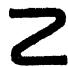
\includegraphics[keepaspectratio]{images/part002_77aeac5d.jpg}}

读者应当警惕，不要以为映射 \((x, y) \to xy\)（一致空间 \(G_{d} \times G_{d}\) 到一致空间 \(G_{d}\) 中的）一般是一致连续的。类似地，对称映射 \(x \to x^{-1}\)（视为 \(G_{d}\) 到 \(G_{d}\) 上的映射时）一般不是一致连续的（见习题 3 与 4）。

命题 3 每个连续同态 \(f\)（拓扑群 \(G\) 到拓扑群 \(G'\) 中的），视为 \(G_d\) 到 \(G_d'\) 中（或 \(G_s\) 到 \(G_s'\) 中）的映射时，是一致连续的。

因为若 \(V'\) 是 \(G'\) 中单位元的一个邻域，且 \(\mathbf{V} = f^{-1}(\mathbf{V}')\)，则关系 \(yx^{-1} \in V\) 蕴含

\[
f (y) (f (x)) ^ {- 1} = f (y x ^ {- 1}) \in V ^ {\prime}.
\]

\subsection{子群、商群与积群上的一致结构}

若 H 是拓扑群 G 的一个子群，则 G 的右一致结构在 H 上诱导的一致结构正是拓扑群 H 的右一致结构。

若 H 是 G 的一个正规子群，且 \(\varphi\) 是 G 到 G/H 上的典范映射，则使 G 中单位元的每个邻域 V 对应于 G/H 的所有偶 \((\dot{x},\dot{y})\)（满足 \(\dot{x}\dot{y}^{-1}\in \varphi (\mathrm{V})\) 的）组成的集，就得到商群 G/H 的右一致结构的一个基本一致邻域系（§ 2 第 6 目命题 17）。这个条件意味着至少有一点 \(x\in \dot{x}\) 且至少有一点 \(y\in \dot{y}\) 使 \(yx^{-1}\in V\){[}即使 \((x,y)\in V_d]\)。特别地，若 N 是 G 的子集 \(\{e\}\) 的闭包，则 G/N 上的右一致结构同构于伴随于 G 上右一致结构的 Hausdorff 一致结构（参看第二章 § 3 第 8 目）。

最后，在拓扑群族 \((\mathbf{G}_{i})\) 的积上，右一致结构是诸 \(G_{i}\) 的右一致结构的积（参看第二章 § 2 第 6 目）。

对左一致结构有类似的结果。

积群 \(\prod_{i\in I}G_i\) 上的左一致结构与右一致结构相同，当且仅当每个因子 \(G_{i}\) 上的左一致结构与右一致结构一致。如果某些 \(G_{i}\) 是交换的而其余的是紧的，情形总如此。

\subsection{完备群}

定义 2 拓扑群称为完备的，如果它的左一致结构与右一致结构都是完备空间的结构。

由第 1 目命题 2，为使一个群是完备的，只需它的两个一致结构之一是完备空间的结构。G 完备当且仅当它的伴随 Hausdorff 群（§ 2 第 6 目）完备。

完备群的每个闭子群是完备的（第二章 § 3 第 4 目命题 8）。完备群的每个积是完备的（第二章 § 3 第 5 目命题 10）。

\pandocbounded{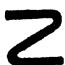
\includegraphics[keepaspectratio]{images/part002_8d186292.jpg}}

另一方面，若 G 是一个完备群且 H 是 G 的一个闭正规子群，则商群 G/H 未必完备（但参看第九章 § 3 第 1 目命题 4）。

命题 4 若在拓扑群 G 中存在 e 的一个邻域 V，它关于右一致结构或左一致结构之一是完备的，则 G 是完备的。

例如设 V 关于右一致结构是完备的，并设 F 是 \(G_{d}\) 上的一个 Cauchy 滤子；则 F 含有一个 \(V_{d}\)-小集 M，且若 \(x_{1} \in M\)，我们因而有 \(M \subset Vx_{1}\)。于是 F 在完备子空间 \(Vx_{1}\)（\(G_{d}\) 的）上的迹是一个 Cauchy 滤子，它收敛于一点 \(x_{0}\)；由于 \(x_{0}\) 是 F 的聚点，它是 F 的极限（第二章 § 3 第 2 目命题 5 推论 2）。

推论 1 局部紧群是完备的。

因为每个紧空间关于它的唯一的一致结构是完备的（第二章 § 4 第 1 目定理 1）。

推论 2 Hausdorff 拓扑群 G 的每个局部紧子群在 G 中是闭的。

因为 Hausdorff 一致空间的每个完备子空间是闭的（第二章 § 3 第 4 目命题 8）。

命题 5 设 \(G_{1}\) 是一个拓扑群，\(G_{2}\) 是一个完备的 Hausdorff 拓扑群，\(H_{1}\)（相应地 \(H_{2}\)）是 \(G_{1}\)（相应地 \(G_{2}\)）的一个稠密子群。则 \(H_{1}\) 到 \(H_{2}\) 中的每个连续同态 u 可以唯一地延拓为一个连续同态 \(\overline{u}\)（\(G_{1}\) 到 \(G_{2}\) 中的）。此外，若 \(G_{1}\) 是 Hausdorff 的且完备的，且 u 是 \(H_{1}\) 到 \(H_{2}\) 上的一个同构，则 \(\overline{u}\) 是 \(G_{1}\) 到 \(G_{2}\) 上的一个同构。

\(\overline{u}\) 关于 \(\mathbf{H}_1\) 与 \(\mathbf{H}_2\) 的右一致结构是一致连续的（第 1 目命题 3），因而容许唯一的延拓：映射 \(\overline{u}\)（\(\mathbf{G}_1\) 到 \(\mathbf{G}_2\) 中的），它关于这些群的右一致结构是一致连续的（第二章 § 3 第 6 目定理 2）。此外，依据恒等延拓原理（第一章 § 8 第 1 目命题 2 推论 1），\(\overline{u}\) 是 \(\mathbf{G}_1\) 到 \(\mathbf{G}_2\) 中的一个同态，由此得到命题的第一个断言。为证明第二个断言，只需考虑同构 \(v\)（\(\mathbf{H}_2\) 到 \(\mathbf{H}_1\) 上的，它是 \(u\) 的逆），以及它的延拓 \(\overline{v}\)（到 \(\mathbf{G}_2\) 到 \(\mathbf{G}_1\) 中的一个连续同态上的）；由于延拓的唯一性，\(\overline{v} \circ \overline{u}\) 与 \(\overline{u} \circ \overline{v}\) 分别是 \(\mathbf{G}_1\) 与 \(\mathbf{G}_2\) 的恒等映射，因而（《集合论》，R，§ 2，第 12 目）\(\overline{u}\) 是双射。

\pandocbounded{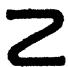
\includegraphics[keepaspectratio]{images/part002_2e6b534c.jpg}}

注。若连续同态 \(u\) 是双射，一般不能推出 \(\overline{u}\) 是单射或满射（参看习题 12）；但参看第 5 目命题 9。

\subsection{拓扑群的完备化}

一致空间 \(G_{d}\) 可以视为它的完备化 \(\hat{G}_{d}\) 的一个稠密子空间。我们将研究 G 能否被视为一个完备 Hausdorff 群 \(G'\) 的一个稠密子群。若能，则一致空间 \(G_{d}'\) 必同构于 \(\hat{G}_{d}\)（第二章 § 3 第 6 目定理 2 的推论），因而我们必须能在 \(\hat{G}_{d}\) 上定义一个拓扑群结构，它在 G 上诱导给定的拓扑群结构。因此我们必须考察：1) 能否把函数 xy 与 \(x^{-1}\) 分别连续延拓到 \(\hat{G}_{d} \times \hat{G}_{d}\) 与 \(\hat{G}_{d}\) 上；2) 这样延拓后的函数是否确实在 \(\hat{G}_{d}\) 上定义一个群结构（这时它们必然在 \(\hat{G}_{d}\) 上定义一个在 G 上诱导给定结构的拓扑群结构）。接着我们要确立：3) 当前面的运算可行时，它们所定义的拓扑群是完备的。最后，我们将看到：4) 若存在一个满足给定条件的完备群，则它在同构意义下是唯一的。

\begin{enumerate}
\def\labelenumi{\arabic{enumi})}
\tightlist
\item
  把 \(xy\) 与 \(x^{-1}\) 连续延拓。由于函数 \(xy\) 与 \(x^{-1}\) 一般不是一致连续的，我们不能应用一致连续函数的延拓定理（第二章 § 3 第 6 目定理 2）。尽管如此，凭第二章 § 3 第 6 目命题 11 以及下面的命题，我们可以延拓 \(xy\)：
\end{enumerate}

命题 6 设 \(\mathfrak{F}\) 与 \(\mathfrak{G}\) 是 \(\mathbf{G}_d\) 上的两个 Cauchy 滤子。则滤子 \(\mathfrak{F} \times \mathfrak{G}\) 在映射 \((x, y) \to xy\) 下的像是 \(\mathbf{G}_d\) 上的一个 Cauchy 滤子基。让我们估计 \(xy\) 与 \(x'y'\) 在 \(\mathbf{G}_d\) 中的“接近程度”；换言之，让我们作乘积 \((x'y')(xy)^{-1} = x'y'y^{-1}x^{-1}\)。对每个 \(a \in \mathbf{G}\)，我们还可以写 \((x'y')(xy)^{-1} = (x'a^{-1})(ay'y^{-1}a^{-1})(ax^{-1})\)。我们将看到，通过适当选取 \(a\)，只要偶 \((x, y)\) 与 \((x', y')\) 属于 \(\mathfrak{F} \times \mathfrak{G}\) 的一个充分小的集，这个乘积的三个因子中的每一个都很小。设 V 是 \(e\) 在 G 中的任一邻域；则存在一个 \(\mathbf{V}_d\)-小集 A ∈ \(\mathfrak{F}\)。在 A 中选取 \(a\)，则若 \(x\) 与 \(x'\) 是 A 的任意两点，我们有 \(x'a^{-1} \in V\) 与 \(ax^{-1} \in V\)。另一方面，关系 \(ay'y^{-1}a^{-1} \in V\) 等价于

\[
y ^ {\prime} y ^ {- 1} \in a ^ {- 1} \mathrm{V}a = \mathrm{W},
\]

而由于 W 是 e 的一个邻域，存在一个 \(W_{d}\)-小集 \(B \in \mathfrak{G}\)。于是对 A × B 中所有 \((x, y)\) 与 \((x', y')\)，我们有 \((x'y')(xy)^{-1} \in V^{3}\)，证毕。

为使 \(x^{-1}\) 可以连续延拓到 \(\hat{G}_d\) 上，充要条件是：在对称映射 \(x \to x^{-1}\) 下，一个 Cauchy 滤子（\(G_d\) 上的）的像是 \(G_d\) 上的一个 Cauchy 滤子（第二章 § 3 第 6 目命题 11）。存在一些拓扑群，这个条件在其中不满足（参看第十章 § 3 习题 16）；在本证明的余下部分我们将假设它满足。

\begin{enumerate}
\def\labelenumi{\arabic{enumi})}
\setcounter{enumi}{1}
\item
  延拓后的函数 \(xy\) 与 \(x^{-1}\) 在 \(\hat{G}_d\) 上定义一个群结构。因为若把恒等延拓原理（第一章 § 8 第 1 目命题 2 推论 1）应用于函数 \(x(yz)\) 与 \((xy)z\)（它们定义在 \(\hat{G}_d \times \hat{G}_d \times \hat{G}_d\) 上且在稠密子空间 \(G_d \times G_d \times G_d\) 上相等），我们就看出合成法则 \((x, y) \to xy\) 在 \(\hat{G}_d\) 上是结合的。出于同样的理由，函数 \(x, ex, xe\) 在 \(\hat{G}_d\) 上相同，且函数 \(e, xx^{-1}, x^{-1}x\) 在 \(\hat{G}_d\) 上相同。
\item
  拓扑群 \(\hat{\mathbf{G}}_d\) 是完备的。设 \(\mathfrak{U}_d\) 是它的右一致结构，\(\mathfrak{U}\) 是 \(\hat{\mathbf{G}}_d\) 上的由 \(\mathbf{G}\) 的右一致结构的完备化所得的一致结构。则 \(\mathfrak{U}\) 与 \(\mathfrak{U}_d\) 在 \(\mathbf{G}\) 上诱导相同的一致结构，因而每个 Cauchy 滤子基 \(\mathfrak{B}\)（\(\mathbf{G}\) 上的，关于 \(\mathfrak{U}_d\) 的）也是关于 \(\mathfrak{U}\) 的一个 Cauchy 滤子基。现在 \(\mathfrak{B}\) 在 \(\hat{\mathbf{G}}_d\) 中收敛，因为 \(\mathcal{U}\) 是一个完备一致结构；且由于 \(\mathcal{U}\) 与 \(\mathcal{U}_d\) 在 \(\hat{\mathbf{G}}_d\) 上诱导相同的拓扑，可知（第二章 § 3 第 4 目命题 9）\(\mathcal{U}_d\) 是一个完备一致结构。这个结论还表明 \(\mathcal{U}\) 与 \(\mathcal{U}_d\) 相同（第二章 § 3 第 6 目定理 2 的推论）。
\item
  唯一性。这由第 3 目命题 5 得出。
\end{enumerate}

概括起来，我们证明了下面的定理：

定理 1 Hausdorff 拓扑群 G 同构于一个完备群 \(\hat{G}\) 的一个稠密子群，当且仅当关于 G 的右一致结构的一个 Cauchy 滤子在对称映射 \(x \to x^{-1}\) 下的像是关于这个一致结构的一个 Cauchy 滤子。完备群 \(\hat{G}\)（它称为 G 的完备化）这时是唯一的（在同构意义下）。

命题 7 设 G 是一个具有完备化 \(\hat{G}\) 的 Hausdorff 拓扑群。则 G 中单位元的诸邻域在 \(\hat{G}\) 中的闭包构成 \(\hat{G}\) 中单位元的一个基本邻域系。

由于 \(\hat{G}\) 是正则的，\(\hat{G}\) 中单位元的每个邻域含有 e 在 \(\hat{G}\) 中的一个开邻域 U 的闭包 V，而 V 也是 U 在 G 上的迹的闭包。

设 G 是一个未必 Hausdorff 的群；设 \(N = \overline{e}\)，\(G' = G/N\) 是伴随于 G 的 Hausdorff 群（§ 2 第 6 目）。若 \(G'\) 有一个完备化 \(\hat{G}'\)，这个完备化称为 G 的 Hausdorff 完备化，记作 \(\hat{G}\)；这时 \(\hat{G}_{d}'\)（相应地 \(\hat{G}_{s}'\)）是一致空间 \(G_{d}\)（相应地 \(G_{s}\)）的 Hausdorff 完备化（第二章 § 3 第 7 目）。

命题 8 设 G 是一个具有 Hausdorff 完备化 \(\hat{G}'\) 的拓扑群。则 G 到一个完备 Hausdorff 群 H 中的每个连续同态 \(u\) 可以唯一地分解为 \(u = v \circ \varphi\)，其中 \(v\) 是 \(\hat{G}'\) 到 H 中的一个连续同态，而 \(\varphi\) 是 G 到 \(\hat{G}'\) 中的典范映射（G' 到 \(\hat{G}'\) 中的典范单射与 G 到 G/N = G' 上的典范同态 \(\psi\) 的复合）。

由于 \(u\) 的核是闭的且含有 \(e\)，它含有 \(N\)，因而 \(u\) 可以写作 \(u = w \circ \psi\)，其中 \(w\) 是 \(G'\) 到 \(H\) 中的一个连续同态；现在对 \(w\) 应用第 3 目命题 5。

\subsection{交换拓扑群的一致结构与完备化}

我们已经指出，在交换拓扑群 G 上左一致结构与右一致结构相同；每当我们谈到 G 的一致结构时，所指的就是这个唯一的一致结构。

定理 2 设 G 是一个交换拓扑群。则函数 \(x^{-1}\) 与 xy 分别在 G 与 G × G 上一致连续。此外 G 容许一个 Hausdorff 完备化 \(\hat{G}\)，且 \(\hat{G}\) 是交换的。

\(x^{-1}\) 的一致连续性由第 1 目命题 2 得出，而 xy 的一致连续性由第 1 目命题 3 得出，因为 \((x, y) \to xy\) 是 \(G \times G\) 到 G 中的一个连续同态。若 G 是 Hausdorff 的，它满足第 4 目定理 1 的条件（如同每个左一致结构与右一致结构相同的 Hausdorff 群一样）；此外由恒等延拓原理，函数 xy 与 yx 在 \(\hat{G} \times \hat{G}\) 上相等；由此得到定理的第二部分，办法是在一般情形考虑伴随于 G 的 Hausdorff 群。

特别地，由这个定理可得：若 \(f\) 与 \(g\) 是一致空间 \(\mathbf{X}\) 到一个交换群 \(G\)（以加法记的）中的两个一致连续映射，则函数 \(-f\) 与 \(f + g\) 是一致连续的。

命题 9 设 G 是一个交换群，\(\mathfrak{T}_1\)、\(\mathfrak{T}_2\) 是与 G 的群结构相容的两个 Hausdorff 拓扑。设 \(\mathfrak{T}_1\) 比 \(\mathfrak{T}_2\) 细，且存在关于 \(\mathfrak{T}_1\) 的 o 的一个基本邻域系，它的成员对 \(\mathfrak{T}_2\) 是闭的。设 \(\mathrm{G}_1, \mathrm{G}_2\) 分别是 G 关于拓扑 \(\mathfrak{T}_1, \mathfrak{T}_2\) 的完备化，\(f: \mathrm{G}_1 \to \mathrm{G}_2\) 是延拓 G 的恒等映射的连续同态（第 3 目命题 5）。则 \(f\) 是单射。

设 G 以加法记。设 \(\mathfrak{U}_{1}\) 是 G 上（依第 1 目）对应于拓扑 \(\mathfrak{T}_{1}\) 的一致结构：只需证明若 F 与 \(F'\) 是关于 \(\mathfrak{U}_{1}\) 的两个极小 Cauchy 滤子（第二章 § 3 第 2 目），它们在 \(G_{2}\) 中收敛于同一点 a，则 \(F = F'\)（第二章 § 3 第 7 目）。为此，只需证明 \(F \cap F'\) 是关于 \(\mathfrak{U}_{1}\) 的一个 Cauchy 滤子。设 V 是 G 中关于 \(\mathfrak{T}_{1}\) 的 o 的一个邻域，使得 V 在 \(\mathfrak{T}_{2}\) 中是闭的，又设 W 是 G 中关于 \(\mathfrak{T}_{1}\) 的 o 的一个对称邻域，使得 \(W + W \subset V\)。由假设，存在一个 \(W_{d}\)-小集 M（相应地 \(M'\)），它属于 F（相应地 \(F'\)）；若 \(x \in M\) 且 \(y \in M\)，我们有 \(y - x \in W\)，即 \(y \in x + W\)。若 \(\overline{W}\) 与 \(\overline{V}\) 是 W 与 V 在 \(G_{2}\) 中的闭包，则由此可得 \(y \in x + \overline{W}\)，因而由于 a 在 M 的闭包中，\(a \in x + \overline{W}\) 对每个 \(x \in M\) 成立。类似地，\(a \in x' + \overline{W}\) 对每个 \(x' \in M'\) 成立，于是 \(x - x' \in \overline{W} + \overline{W}\)；但由 \((x, y) \to x + y\) 是 \(G_{2} \times G_{2}\) 到 \(G_{2}\) 中的一个连续映射，我们有 \(\overline{W} + \overline{W} \subset \overline{W + W} \subset \overline{V}\)。由此可得，若 \(x \in M\) 且 \(x' \in M'\)，则 \(x - x' \in \overline{V} \cap G = V\)，因为 V 在 \(\mathfrak{T}_{2}\) 中是闭的；证毕。

推论 1 在命题 9 的假设下，若 A 是 G 的一个子集，它关于一致结构 \(\mathfrak{U}_{2}\)（对应于 \(\mathfrak{T}_{2}\) 的）是一个完备子空间，则 A 关于一致结构 \(\mathfrak{U}_{1}\)（对应于 \(\mathfrak{T}_{1}\) 的）也是一个完备子空间。

若 \(A_{1}\) 是 A 在 \(G_{1}\) 中的闭包，则 \(f(A_{1})\) 含于 A 在 \(G_{2}\) 中的闭包，而由假设这个闭包等于 A。由于依定义 \(f(A)=A\) 且 f 是单射，我们有 \(A_{1}=A\)。

推论 2 设 G 是一个交换群，\(\mathfrak{T}_1, \mathfrak{T}_2\) 是与 G 的群结构相容的两个拓扑。设 \(\mathfrak{T}_1\) 比 \(\mathfrak{T}_2\) 细，且存在 o 的一个基本邻域系 \(\mathfrak{B}\)（关于 \(\mathfrak{T}_1\) 的），它的成员关于一致结构 \(\mathfrak{U}_2\)（对应于 \(\mathfrak{T}_2\) 的）是完备的。则 G 关于一致结构 \(\mathfrak{U}_1\)（对应于 \(\mathfrak{T}_1\) 的）是完备的。

\(\mathfrak{B}\) 中的诸集在拓扑 \(\mathfrak{T}_{2}\) 中是闭的，因而由推论 1 关于一致结构 \(\mathfrak{U}_{1}\) 是完备的；于是结论由第 3 目命题 4 得出。

\section{逆紧作用于拓扑空间的群；拓扑群与带算子空间中的紧性}

\subsection{逆紧作用于拓扑空间的群}

定义 1 设 G 是连续作用在拓扑空间 X 上的一个拓扑群。如果映射

\[
\theta : (s, x) \rightarrow (x, s. x) \text{ 从 } \mathbf{G} \times \mathbf{X} \text{ 到 } \mathbf{X} \times \mathbf{X}
\]

是逆紧的（第一章 § 10 第 1 目定义 1），就称 G 逆紧作用在 X 上。

设 \(\Gamma \subset \mathbf{G} \times \mathbf{X} \times \mathbf{X}\) 是映射 \(\rho: (s, x) \to s.x\) 的图。由于 \(\rho\) 连续，映射 \(\sigma: (s, x) \to (s, x, s.x)\) 是 \(\mathbf{G} \times \mathbf{X}\) 到 \(\Gamma\) 上的一个同胚，且复合映射

\[
\mathbf {G} \times \mathbf {X} \xrightarrow {\sigma} \Gamma \xrightarrow {\mathrm{pr} _ {2 3}} \mathbf {X} \times \mathbf {X}
\]

就是 \(\theta\)。因此定义 1 等价于说 \(\operatorname{pr}_{23}\) 在 \(\Gamma\) 上的限制是 \(\Gamma\) 到 \(\mathbf{X} \times \mathbf{X}\) 中的一个逆紧映射。

第一章 § 10 第 2 目定理 1 表明，G 逆紧作用在 X 上，当且仅当下列条件满足：

对每个由超滤子 F 过滤的集 A，以及每个映射

\[
\alpha \rightarrow (s _ {\alpha}, x _ {\alpha})
\]

（A 到 \(\mathbf{G} \times \mathbf{X}\) 中的），如果映射 \(\alpha \to (s_{\alpha}.x_{\alpha}, x_{\alpha})\) 有一个极限 \((b, a)\)（关于 \(\mathfrak{F}\) 的），则 \(\alpha \to s_{\alpha}\) 有一个极限 \(t \in \mathbf{G}\)（关于 \(\mathfrak{F}\) 的），使得 \(t.a = b\)。

例。1) 设 H 是拓扑群 G 的一个闭子群。若 G 逆紧作用在 X 上，则 H 也逆紧作用在 X 上，因为 H × X 在 G × X 中是闭的（第一章 § 10 第 1 目命题 5 推论 1）。例如若取 X = G，G 通过左平移作用在自身上，则映射 G × X → X × X 是一个同胚，因而是逆紧的；于是 H 通过左平移逆紧作用在 G 上。

\begin{enumerate}
\def\labelenumi{\arabic{enumi})}
\setcounter{enumi}{1}
\tightlist
\item
  若 G 逆紧作用在 X 上，则它逆紧作用在 X 的每个子空间 \(X'\)（它是 X 的点的轨道的并）上（换言之，\(X'\) 关于由 G 定义的等价关系是饱和的）。因为 \(X' \times X'\) 在 \(G \times X\) 中的原像是 \(G \times X'\)，且我们可以应用第一章 § 10 第 1 目命题 3。
\end{enumerate}

命题 1 设 G 是连续作用在拓扑空间 X 上的一个拓扑群，K 是 G 的一个拟紧子集。则映射 \(\rho: (s, x) \to s.x\)（\(K \times X\) 到 \(X\) 中的）是逆紧的。

\(\rho\) 分解为 \(\mathbf{K} \times \mathbf{X} \to \mathbf{K} \times \mathbf{X} \xrightarrow{\mathrm{pr}_2} \mathbf{X}\)，其中 \(\alpha(s, x) = (s, s.x)\)。\(\alpha\) 是一个同胚，因为 \(\alpha^{-1}: (s, y) \to (s, s^{-1}.y)\) 连续。由于 \(\mathbf{K}\) 是拟紧的，\(\mathrm{pr}_2\) 是逆紧的（第一章 § 10 第 2 目定理 1 推论 5）；因而 \(\rho\) 是逆紧的（第一章 § 10 第 1 目命题 5）。

推论 1 若 A 是 X 的一个闭（相应地紧）子集，则 K.A 在 X 中是闭的（相应地，若 X 是 Hausdorff 的，则是紧的）。

关于闭集的断言由命题 1 以及逆紧映射是闭映射这一事实（第一章 § 10 第 1 目命题 1）得出。关于紧集的断言是显然的。

\pandocbounded{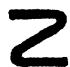
\includegraphics[keepaspectratio]{images/part002_62417fce.jpg}}

应当注意，若 L 是 X 的一个紧子集，F 是 G 的一个闭子集，则 F. L 在 X 中未必是闭的（§ 2 习题 29；参看第 5 目命题 12 的推论）。

推论 2 若 K 是拓扑群 G 的一个拟紧子群，则等价关系 \(x^{-1}y \in K\) 是闭的，且典范映射 \(\varphi: G \to G/K\) 是逆紧的。

第一个断言由推论 1 应用于通过右平移作用在自身上的 G 得出，第二个断言则由第一章 § 10 第 2 目定理 1 得出。

推论 3 设 K 是拓扑群 G 的一个拟紧正规子群，\(\varphi\) 是典范映射 G → G/K。则对 G 的每个闭子群 A，A/A∩K 到 \(\varphi(A)\) 上的典范双射是拓扑群的一个同构。

由于 \(x^{-1}y \in K\) 是一个闭等价关系（推论 2），本推论由第一章 § 5 第 2 目命题 4 得出。

命题 2 设 K 是连续作用在 Hausdorff 空间 X 上的一个紧群。则：

\begin{enumerate}
\def\labelenumi{\alph{enumi})}
\item
  K 逆紧作用在 X 上。
\item
  映射 \((s, x) \to s.x\)（\(\mathbf{K} \times \mathbf{X}\) 到 \(\mathbf{X}\) 中的）是逆紧的。
\item
  X 到 X/K 上的典范映射是逆紧的。
\item
  是命题 1 的推论。至于 a)，由于 K 是紧的，\(\operatorname{pr}_{2}:(s,x)\to x\) 是逆紧的（第一章 § 10 第 2 目定理 1 推论 5）；因而，由于 X 是 Hausdorff 的，\((s,x)\to(x,s.x)\) 是逆紧的（第一章 § 10 第 1 目命题 5 推论 3）。剩下证明 c)。依命题 1 的推论 1，典范映射 \(\varphi:X\to X/K\) 是闭的。若 Z 是任一拓扑空间且让 K 平凡作用在 Z 上，则 K 连续作用在 \(X\times Z\) 上，因而典范映射 \(X\times Z\to(X\times Z)/K\) 是闭的。但 \((X\times Z)/K\) 可以典范地等同于 \((X/K)\times Z\)（§ 2 第 4 目引理 2 及第一章 § 5 第 3 目命题 8 的推论）；因而典范映射 \(X\times Z\to(X\times Z)/K\) 可以等同于 \(\varphi\times1\)，且由于它对所有 Z 是闭的，可知 \(\varphi\) 是逆紧的。
\end{enumerate}

推论 1 在命题 2 的假设下，X 是紧的（相应地局部紧的），当且仅当 X/K 是紧的（相应地局部紧的）。

这由典范映射 \(X \rightarrow X/K\) 是逆紧的这一事实得出，依据第一章 § 10 第 4 目命题 9。

推论 2 设 G 是一个 Hausdorff 拓扑群，K 是 G 的一个紧子群。则 G 是紧的（相应地局部紧的），当且仅当 G/K 是紧的（相应地局部紧的）。

对通过右平移作用在 G 上的 K 应用推论 1。
% semantic-fragments: legacy-input-seam
\relax{}
\subsection{群作逆紧作用的性质}

命题 3. 若拓扑群 G 逆紧作用于拓扑空间 X，则轨道空间 X/G 是豪斯多夫的。若 G 还是豪斯多夫的，则 X 也是豪斯多夫的。

设 \(C \subset X \times X\) 是等价关系 \(R\)（由 \(G\) 定义在 \(X\) 上的）的图；则 \(C\) 是 \(G \times X\) 在映射 \(\theta : (s, x) \to (x, s.x)\) 下的像。由于 \(\theta\) 是逆紧的，\(C\) 在 \(X \times X\) 中闭（第一章，§ 10，第 1 节，命题 1）。由于关系 \(R\) 是开的（§ 2，第 4 节，引理 2），由此推出 \(X/G\) 是豪斯多夫的（第一章，§ 8，第 3 节，命题 8）。

现在设 G 是豪斯多夫的。则映射 \(x \to (e, x)\)（X 到 \(G \times X\) 中的映射）是 X 到 \(G \times X\) 的一个闭子空间上的同胚，因而是逆紧的（第一章，§ 10，第 1 节，命题 2）。把这个映射与映射 \((s, x) \to (x, s.x)\)（\(G \times X\) 到 \(X \times X\) 中的映射，由假设它是逆紧的）复合，就得到 X 到 \(X \times X\) 中的一个逆紧映射，即对角映射 \(x \to (x, x)\)。于是对角线 \(\Delta\)（\(X \times X\) 的对角线）在 X 中是闭的，因此 X 是豪斯多夫的。

命题 4. 设 G 是逆紧作用于拓扑空间 X 的一个拓扑群，并设 x 是 X 的一点。用 G.x 表示 x 的轨道，用 \(K_{x}\) 表示 x 的稳定子群。那么：

\begin{enumerate}
\def\labelenumi{\alph{enumi})}
\item
  映射 \(s \to s.x\) 是 \(G\) 到 \(X\) 中的逆紧映射。
\item
  \(\mathbf{K}_x\) 是拟紧的。
\item
  \(\mathbf{G} / \mathbf{K}_x\) 到 \(\mathbf{G}.x\) 上的典范映射是同胚。
\item
  轨道 G.x 在 X 中是闭的。
\end{enumerate}

\(\{x\} \times X\) 在 \(\theta : (s, x) \to (x, s.x)\) 下的逆像是 \(G \times \{x\}\)；因此，由第一章 § 10 第 1 节命题 3，\(\theta\) 在 \(G \times \{x\}\) 上的限制是 \(G \times \{x\}\) 到 \(\{x\} \times X\) 中的逆紧映射，由此得 a)。由于 \(K_x\) 是 \(x\) 在 \(s \to s.x\) 下的逆像，故 b) 由第一章 § 10 第 2 节定理 1 得出。c) 与 d) 是 a) 的推论，这依据第一章 § 10 第 1 节命题 2 与命题 5 b)。

注. 命题 4 表明，若拓扑群 G 逆紧作用于齐性空间 G/H，则子群 H 是拟紧的（从而当 G 是豪斯多夫的时它是紧的）。可以证明，这也是 G 逆紧作用于 G/H 的一个充分条件（习题 3）。

命题 5. 设 G（相应地，G'）是连续作用于拓扑空间 X（相应地，X'）的拓扑群。设 φ 是 G 到 \(\mathbf{G}'\) 中的一个连续同态，并设 \(\psi\) 是 X 到 \(\mathbf{X}'\) 中与 \(\varphi\) 相容的连续映射（ \(\S 2\) ，第 4 节）。那么：

\begin{enumerate}
\def\labelenumi{(\roman{enumi})}
\item
  若 \(\varphi\) 是满射，\(\psi\) 是满射且逆紧的，并且 \(\mathbf{G}\) 逆紧作用于 \(\mathbf{X}\)，则 \(\mathbf{G}'\) 逆紧作用于 \(\mathbf{X}'\)。
\item
  若 \(\varphi\) 是逆紧的，\(\mathbf{G}'\) 逆紧作用于 \(\mathbf{X}'\)，且 \(\mathbf{X}\) 是豪斯多夫的，则 \(\mathbf{G}\) 逆紧作用于 \(\mathbf{X}\)。
\end{enumerate}

为证 (i)，考虑交换图

\[
\begin{array}{c c c c} \mathbf {G} & \times \mathbf {X} \xrightarrow {\theta} \mathbf {X} & \times \mathbf {X} \\ \alpha & \downarrow & & \downarrow \beta \\ \mathbf {G} ^ {\prime} & \times \mathbf {X} ^ {\prime} \xrightarrow {\theta^ {\prime}} \mathbf {X} ^ {\prime} & \times \mathbf {X} ^ {\prime} \end{array}
\]

其中 \(\alpha = \varphi \times \psi\)，\(\beta = \psi \times \psi\)。由假设，\(\theta\) 是逆紧的；\(\beta\) 也是逆紧的{[}第一章，§ 10，第 1 节，命题 4a){]}；于是 \(\beta \circ \theta = \theta' \circ \alpha\) 是逆紧的{[}第一章，§ 10，第 1 节，命题 5a){]}。由于 \(\alpha\) 是满射，由此推出 \(\theta'\) 是逆紧的{[}第一章，§ 10，第 1 节，命题 5b){]}。

为证 (ii)，考虑超滤子 \(\mathfrak{U}\)，它定义在 \(\mathbf{G} \times \mathbf{X}\) 上，使得映射

\[
(s, x) \rightarrow s. x \quad \text { and } \quad (s, x) \rightarrow x
\]

关于 \(\mathfrak{U}\) 分别收敛于 \(y_0\) 与 \(x_0\)。由此推出 \((s, x) \to \varphi(s). \psi(x)\) 与 \((s, x) \to \psi(x)\) 关于 \(\mathfrak{U}\) 收敛。由于 \(\mathbf{G}'\) 逆紧作用于 \(\mathbf{X}'\)，这就意味着（第 1 节）\((s, x) \to \varphi(s)\) 关于 \(\mathfrak{U}\) 收敛于一点 \(s_0' \in \mathbf{G}'\)。由于 \(\varphi\) 是逆紧的，我们推出（第一章，§ 10，第 2 节，定理 1）\((s, x) \to s\) 关于 \(\mathfrak{U}\) 收敛于一点 \(s_0 \in \mathbf{G}\)。于是在 \(\mathbf{X}\) 中极限的唯一性表明 \(y_0 = s_0 x_0\)，从而 \(\mathbf{G}\) 逆紧作用于 \(\mathbf{X}\)（第 1 节）。

\subsection{在拓扑空间上自由作用的群}

定义 2. 设 G 是作用于一个集合 X 上的群。如果 X 的每个元素的稳定子群都是 \(\{e\}\)，换句话说，如果关系 \(s.x = x, s \in G, x \in X\) 蕴含 s = e，则称 G 自由作用于 X。

例. 设 G 是群，H 是 G 的子群。则 H 通过（左或右）平移自由作用于 G。

设 G 是自由作用于集合 X 的群，R 是 G 在 X 上定义的等价关系，\(C \subset X \times X\) 是 R 的图。若 \((x, y) \in C\)，则存在 \(s \in G\) 使得 s.x = y；且 s 是唯一的，因为 \(s.x = s'.x\) 蕴含 \(s'^{-1}s.x = x\)，从而 \(s'^{-1}s = e\)（由于 G 自由作用）。让 \((x, y) \in C\) 对应于使 s.x = y 的唯一的 \(s \in G\)，我们就定义了一个映射 \(\varphi: C \to G\)，我们称它为 C 到 G 中的典范映射。采用此记号：

命题 6. 设 G 是连续作用于拓扑空间 X 的拓扑群，且设 G 自由作用于 X。则 G 逆紧作用于 X 当且仅当下述条件成立：

(FP) 由 G 所定义的等价关系的图 C 在 \(X \times X\) 中闭，且典范映射 \(\varphi: C \rightarrow G\) 连续。

集合 C 是映射 \(\theta: (s, x) \to (x, s.x)\)（\(\mathbf{G} \times \mathbf{X}\) 到 \(\mathbf{X} \times \mathbf{X}\) 中的映射）的像。我们知道（第一章，§ 10，第 1 节，命题 2），\(\theta\) 是逆紧的当且仅当 C 在 \(\mathbf{X} \times \mathbf{X}\) 中闭，并且（若用 \(\theta'\) 表示把 \(\theta\) 看作 \(\mathbf{G} \times \mathbf{X}\) 到 C 中的映射）\(\theta'\) 是同胚。现在，假设蕴含 \(\theta'\) 是双射且其逆是映射 \((x, y) \to (\varphi(x, y), x)\)。于是 \(\theta'\) 是同胚当且仅当 \(\varphi\) 连续。

\subsection{作逆紧作用的局部紧群}

命题 7. 设 G 是连续作用于豪斯多夫空间 X 的局部紧群。则 G 逆紧作用于 X 当且仅当：对 X 的每一对点 x, y，存在 x 的邻域 \(V_{x}\) 与 y 的邻域 \(V_{y}\)，使得集合 K——由 \(s \in G\) 中满足 \(s \cdot V_{x} \cap V_{y} \neq \emptyset\) 的所有 s 组成——在 G 中相对紧。

设 F 是把无穷远点 \(\omega\) 添加到 G 上所得的紧空间，并设 \(\Gamma\) 是 \(\rho: (s, x) \to s.x\) 的图，把它看作 \(F \times X \times X\) 的一个子集。我们来证明，如果 \(pr_{23}\) 在 \(\Gamma\) 上的限制是逆紧的，那么 \(\Gamma\) 在 \(F \times X \times X\) 中是闭的。事实上，这一假设蕴含映射 \(u: (t, s, x, y) \to (t, x, y)\)（\(F \times \Gamma\) 到 \(F \times X \times X\) 中的映射）是闭映射。若 \(\Gamma'\) 是由点 \((s, s)\) 组成的集合，这些点位于 \(F \times G\) 中且 \(s \in G\)，则 \(\Gamma'\) 在 \(F \times G\) 中闭，因为它是典范单射 \(G \to F\) 的图（第一章，§8，第 1 节，命题 2 的推论 2）；于是交 \((\Gamma' \times X \times X) \cap (F \times \Gamma)\) 在 \(F \times \Gamma\) 中闭，并且立即可以看出它在 u 下的像正是把 \(\Gamma\) 看作 \(F \times X \times X\) 的子集时的那个集合；从而 \(\Gamma\) 在 \(F \times X \times X\) 中闭。另一方面，我们有 \((\{\omega\} \times X \times X) \cap \Gamma = \emptyset\)。于是由 F 的定义，对每一点 \((x, y) \in X \times X\)，存在 \((x, y)\) 在 \(X \times X\) 中的一个邻域 W 和 G 的一个紧子集 K，使得

\[
((\mathbf {G} - \mathbf {K}) \times \mathbf {W}) \cap \Gamma ;
\]

为空；由于可取 W 为形如 \(V_{x} \times V_{y}\) 的邻域，其中 \(V_{x}\) 与 \(V_{y}\) 分别是 X 中 x 与 y 的邻域，断言“((G - K) × W) ∩ Γ = ∅”就成为“若 s∉K，则 s.Vx∩Vy=∅”。这样我们就证明了命题所述条件的必要性。反之，设此条件成立；设 A 是由超滤子 \(\mathfrak{F}\) 滤化的集合，并设 \(\alpha \to (s_{\alpha}, x_{\alpha})\) 是 A 到 \(G \times X\) 中的映射，使得 \(\lim_{\mathfrak{F}} x_{\alpha} = x\) 且 \(\lim_{\mathfrak{F}} s_{\alpha}\cdot x_{\alpha} = y\)。设 K、Vx 与 Vy 满足命题的条件。由假设，存在集合 \(M \in \mathfrak{F}\)，使得若 \(\alpha \in M\)，则 \(x_{\alpha} \in V_{x}\) 且 \(s_{\alpha}\cdot x_{\alpha} \in V_{y}\)，从而 \(s_{\alpha} \in K\)。这表明 \(\alpha \to s_{\alpha}\) 关于 \(\mathfrak{F}\) 收敛，证毕。

若 G 是紧的，命题 7 的条件平凡地成立；这样我们重新得到命题 2a)。

命题 7 特别表明，连续作用于豪斯多夫空间 X 的离散群 G 逆紧作用于 X 当且仅当：对 X 的每一对点 \((x, y)\)，存在 x 的邻域 \(V_{x}\) 与 y 的邻域 \(V_{y}\)，使得由 \(s \in G\) 中满足 \(s \cdot V_{x} \cap V_{y} \neq \emptyset\) 的点组成的集合是有限的。

命题 8. 设 G 是逆紧作用于豪斯多夫空间 X 的离散群。设 x 是 X 的一点，\(K_{x}\) 是 x 的稳定子群。那么：

\begin{enumerate}
\def\labelenumi{\alph{enumi})}
\item
  子群 \(K_{x}\) 是有限的，并且存在 \(U \subset X\) 的开集，它包含 x，在 \(K_{x}\) 下稳定，并且在它上面由 G 所定义的关系诱导的等价关系就是由 \(K_{x}\) 定义的等价关系。
\item
  典范映射 \(\mathbf{U} / \mathbf{K}_x\to \mathbf{X} / \mathbf{G}\) 是 \(\mathbf{U} / \mathbf{K}_x\) 到 \(x\) 的类在 \(\mathbf{X} / \mathbf{G}\) 中的一个开邻域上的同胚。
\end{enumerate}

由命题 7，\(\mathbf{K}_x\) 是有限的。为构造满足所需条件的开集 \(\mathbf{U}\)，首先注意，由命题 7 存在开集 \(\mathrm{U}_0\)（包含 \(x\)），使得集合 \(\mathbf{K}\)——由 \(s \in \mathbf{G}\) 中满足 \(s. \mathrm{U}_0 \cap \mathrm{U}_0 \neq \emptyset\) 的那些 s 组成——是有限的。显然 \(\mathbf{K}_x \subset \mathbf{K}\)；设 \(s_1, \ldots, s_n\) 是 \(\mathbf{K} - \mathbf{K}_x\) 的元素。若令 \(x_i = s_i.x\)（ \(1 \leqslant i \leqslant n\)），则 \(x_i \neq x\) 对每个 \(i\) 成立；由于 \(\mathbf{X}\) 是豪斯多夫的，对每个指标 \(i\) 存在开邻域 \(\mathrm{V}_i\)（包含 \(x\)）与开邻域 \(\mathrm{V}_i'\)（包含 \(s_i.x\)），使得 \(\mathrm{V}_i \cap \mathrm{V}_i' = \emptyset\)。令 \(\mathrm{U}_i = \mathrm{V}_i \cap s_i^{-1}. \mathrm{V}_i'\)；则 \(\mathrm{U}_i\) 显然是开的且包含 \(x\)，并且我们有 \(\mathrm{U}_i \cap s_i. \mathrm{U}_i \subset \mathrm{V}_i \cap \mathrm{V}_i' = \emptyset\)。令 \(\mathrm{U}' = \mathrm{U}_0 \cap \mathrm{U}_1 \cap \ldots \cap \mathrm{U}_n\)；\(\mathrm{U}'\) 是开的，包含 \(x\)，并且 \(\mathrm{U}' \cap s. \mathrm{U}' = \emptyset\) 对 \(s \notin \mathbf{K}_x\) 成立。令 \(\mathrm{U} = \bigcap_{t \in \mathbf{K}_x} t. \mathrm{U}'\)，我们最终得到一个开集，它在 \(\mathbf{K}_x\) 下稳定，包含 \(x\)，并且 \(\mathrm{U} \cap s. \mathrm{U} = \emptyset\) 对 \(s \notin \mathbf{K}_x\) 成立：\(\mathrm{U}\) 就是所要求的开集。

典范映射 \(\mathbf{U} / \mathbf{K}_x\to \mathbf{X} / \mathbf{G}\) 是 \(\mathbf{U} / \mathbf{K}_x\) 到 \(\mathbf{X} / \mathbf{G}\) 中一个开集上的同胚这一事实，由第一章 § 5 第 2 节命题 4 得出，因为 \(\mathbf{U}\) 是开的且由 \(\mathbf{G}\) 定义的等价关系是开的（§ 2，第 4 节，引理 2）。

推论. 若再假设 \(K_{x}=\{e\}\)，则点 x 有一个开邻域 U，使得典范映射 \(X\to X/G\) 在 U 上的限制是 U 到 X/G 的一个开子集上的同胚。

\subsection{连续作用于局部紧空间的群}

命题 9. 设 G 是连续作用于局部紧空间 X 的拓扑群。那么，若 X/G 是豪斯多夫的，则它是局部紧的。

由于 G 在 X 上定义的等价关系是开的（§ 2，第 4 节，引理 2），本命题由第一章 § 10 第 4 节命题 10 得出。

命题 10. 设 G 是连续作用于局部紧空间 X 的拓扑群，且设 X/G 是豪斯多夫的。设 \(\varphi\) 是 X 到 X/G 上的典范映射。那么，若 K' 是 X/G 的任意紧子集，则存在 X 的紧子集 K 使得 \(\varphi(K) = K'\)。

由于由 G 定义的等价关系是开的（§ 2，第 4 节，引理 2），本命题是第一章 § 10 第 4 节命题 10 的特殊情形。

命题 11. 设 G 是逆紧作用于非空空间 X 的豪斯多夫拓扑群。若 X 是紧的（相应地，局部紧的），则 G 与 X/G 也是紧的（相应地，局部紧的）。

由假设，映射 \(\theta : (s, x) \to (x, s.x)\)（\(G \times X\) 到 \(X \times X\) 中的映射）是逆紧的；若 \(X \times X\) 是紧的（相应地，局部紧的），则第一章 § 10 第 4 节命题 9 的推论表明 \(G \times X\) 也是紧的（相应地，局部紧的），从而 \(G\) 也是紧的（相应地，局部紧的），因为 \(X \neq \emptyset\)。由于 \(X/G\) 是豪斯多夫的（第 2 节，命题 3），\(X\) 的紧性（相应地，局部紧性）蕴含 \(X/G\) 的紧性（相应地，局部紧性）{[}第一章，§ 10，第 4 节，命题 8（相应地，命题 9）{]}（见 § 2，习题 29）。

我们现在给出一些判别法，使我们能够断言豪斯多夫拓扑群 G 逆紧作用于局部紧空间 X。对 X 的每一对子集 K, L，我们用 P(K, L) 表示由所有这样的 \(s \in G\) 组成的集合：它们满足 \(s \cdot K \cap L \neq \emptyset\)。

定理 1. 设 G 是连续作用于拓扑空间 X 的豪斯多夫拓扑群。设 K 是 X 的紧子集，L 是 X 的闭子集。那么：

\begin{enumerate}
\def\labelenumi{\alph{enumi})}
\item
  集合 \(\mathbf{P}(\mathbf{K},\mathbf{L})\) 在 \(\mathbf{G}\) 中是闭的。
\item
  若 G 逆紧作用于 X 且 L 是紧的，则 P(K, L) 是紧的。
\item
  反之，若 X 是局部紧的，并且对 X 的每一对紧子集 K, L，P(K, L) 都在 G 中相对紧{[}从而由 a) 是紧的{]}；则 G 逆紧作用于 X（且若 X 非空，则由命题 11，G 是局部紧的）。
\end{enumerate}

映射 \((s, x) \to s.x\)（\(G \times K\) 到 X 中的映射）是连续的，因此 L 在此映射下的逆像 \(L'\) 是闭的。由于 K 是紧的，投影 \(pr_{1}: G \times K \to G\) 是逆紧的（第一章，§ 10，第 2 节，定理 1 的推论 5），因此 \(L'\) 在 \(pr_{1}\) 下的像是闭的。这个像就是 \(P(K, L)\)，于是 a) 得证。

为证 b)：X 是豪斯多夫的（第 2 节，命题 3）。由假设，映射 \(\theta: (s, x) \to (x, s.x)\)（\(G \times X\) 到 \(X \times X\) 中的映射）是逆紧的；由于 \(K \times L\) 是紧的，\(\theta^{-1}(K \times L)\) 也是紧的，因为 \(X\) 是豪斯多夫的（第一章，§ 10，第 2 节，命题 6）。于是 \(P(K, L)\)（\(\theta^{-1}(K \times L)\) 在 \(G\) 中的投影）是紧集。

为证 c)：由于 \(K \times L\) 在 \(X \times X\) 中闭，由此推出 \(\theta^{-1}(K \times L)\) 在 \(P(K, L) \times K\) 中闭，从而在 c) 的假设下是紧的。由于 \(X \times X\) 的每个紧子集都含于形如 \(K \times L\) 的紧子集中，由此推出 \(X \times X\) 的任意紧子集在 \(\theta\) 下的逆像是紧的；又由于 \(X \times X\) 是局部紧的，这就表明 \(\theta\) 是逆紧的（第一章，§ 10，第 3 节，命题 7）{[}见第四章，§ 1，习题 4c){]}。

注. 显然我们有 \(\mathrm{P}(\mathrm{K},\mathrm{L})\subset\mathrm{P}(\mathrm{K}\cup\mathrm{L},\mathrm{K}\cup\mathrm{L})\)；因此，为使 G 逆紧作用于局部紧空间 X，只需对 X 的每个紧子集 K，集合 \(\mathrm{P}(\mathrm{K},\mathrm{K})\) 在 G 中相对紧即可。特别地，离散群 G 逆紧作用于局部紧空间 X 当且仅当：对 X 的每个紧子集 K，由所有这样的 \(s\in G\) 组成的集合是有限的：它们满足 \(s.K\cap K\neq\emptyset\)。

例. * 设 X 是一个复解析流形，解析同构于 \(\mathbf{C}^n\) 的一个有界开子集，并设 G 是 X 的解析自同构群。紧收敛拓扑与 G 的群结构相容，并且可以证明 G 逆紧作用于 X。特别地，G 的每个离散子群都逆紧作用于 X。

例如取 X 为上半平面 \(\mathfrak{J}(z)>0\)，它解析同构于 C 中的一个开圆盘。此时 G 是由所有形如 \(z\to (az+b)/(cz+d)\) 的变换组成的群，其中 \(a,b,c,d\) 是实数且 \(ad-bc\neq0\)。G 中由所有满足 \(a,b,c,d\) 为整数且 \(ad-bc=1\) 的此类变换组成的子群 H 是 G 的离散子群，称为模群。根据上文所述，它逆紧作用于上半平面 \(\mathfrak{J}(z)>0\)。 *

命题 12. 设 G 是连续作用于拓扑空间 X 的豪斯多夫拓扑群。设 K 是 X 的紧子集，并设 \(\rho_{K}\) 是映射 \((s, x) \to s.x\)（\(G \times K\) 到 X 中的映射）。那么：

\begin{enumerate}
\def\labelenumi{\alph{enumi})}
\item
  若 G 逆紧作用于 X，则 \(\rho_{\mathbf{K}}\) 是逆紧的。
\item
  若 X 是局部紧的并且对 X 的每个紧子集 K，\(\rho_{K}\) 都是逆紧的，则 G 逆紧作用于 X。
\end{enumerate}

映射 \(\rho_{\mathbf{K}}\) 可分解为 \(\mathbf{G} \times \mathbf{K} \xrightarrow{\theta_{\mathbf{K}}} \mathbf{K} \times \mathbf{X} \xrightarrow{\mathrm{pr}_2} \mathbf{X}\)，其中 \(\theta_{\mathbf{K}}\) 是 \(\mathbf{G} \times \mathbf{K}\) 上的这样一个限制：被限制的映射是 \(\theta: (s, x) \to (x, s.x)\)（\(\mathbf{G} \times \mathbf{X}\) 到 \(\mathbf{X} \times \mathbf{X}\) 中的映射）。由于 \(\theta^{-1}(\mathbf{K} \times \mathbf{X}) = \mathbf{G} \times \mathbf{K}\)，\(\theta_{\mathbf{K}}\) 在 \(\theta\) 逆紧时是逆紧的（第一章，§ 10，第 1 节，命题 3）。另一方面，由于 \(\mathbf{K}\) 是紧的，投影 \(\mathrm{pr}_2: \mathbf{K} \times \mathbf{X} \to \mathbf{X}\) 是逆紧的（第一章，§ 10，第 2 节，定理 1，推论 5），于是 \(\rho_{\mathbf{K}}\) 是逆紧的（同处，第 1 节，命题 5）。

反之，设 \(\rho_{\mathbf{K}}\) 对每个紧子集 \(\mathbf{K} \subset \mathbf{X}\) 都是逆紧的。若 \(\mathbf{L}\) 是 \(\mathbf{X}\) 的紧子集，则 \(\rho_{\mathbf{K}}^{-1}(\mathbf{L})\) 是 \(\mathbf{G} \times \mathbf{K}\) 的紧子集，它在 \(\mathbf{G}\) 中的投影是 \(\mathrm{P}(\mathbf{K}, \mathbf{L})\)；因此 \(\mathrm{P}(\mathbf{K}, \mathbf{L})\) 是紧的。于是若 \(\mathbf{X}\) 是局部紧的，则由定理 1 推出 \(\mathbf{G}\) 逆紧作用于 \(\mathbf{X}\)。

推论. 设 G 是逆紧作用于拓扑空间 X 的豪斯多夫拓扑群。若 K 是 X 的任意紧子集且 F 是 G 的任意闭子集，则 F.K 在 X 中闭。

这由命题 12 以及第一章 § 10 第 1 节命题 1 得出。

\subsection{局部紧齐性空间}

命题 13. 设 G 是局部紧群，H 是 G 的闭子群。则齐性空间 G/H 是局部紧的且是仿紧的。

由于 G/H 是豪斯多夫的（§ 2，第 5 节，命题 13），把第 5 节命题 9 应用于右作用于 G 的 H，可知它是局部紧的。于是只需再证 G/H 是仿紧的。设 V 是 G 中 e 的对称紧邻域，并设 \(G_{0}=V^{\infty}\) 是由 V 生成的 G 的子群。\(G_{0}\) 是开的（§ 2，第 1 节，命题 4 的推论）且连续作用于 G/H（§ 2，第 5 节，命题 12）。如果我们能证明每个轨道 \(G_{0}.z\)（ \(z\in G/H\)）都是 G/H 的开子集且是紧集的可数并，那么就可推出 G/H 是诸不同轨道 \(G_{0}.z\) 的拓扑和，从而是仿紧的（第一章，§ 9，第 10 节，定理 5）。\(\mathbf{G}_0.z\) 在 G/H 中是开的，这由 \(\mathbf{G}_0\) 在 G 中是开的以及等价关系 \(x^{-1}y\in H\) 是开的（§ 2，第 4 节，引理 2）这两个事实得出。另一方面，\(\mathbf{G}_0.z\) 是诸集合 \(\mathbf{V}^n.z\)（ \(n\geqslant 1\)）的并，且由于 \(\mathbf{V}^n\) 在 G 中紧而 G/H 是豪斯多夫的，\(\mathbf{V}^n.z\) 是紧的。证毕。

命题 14. 在局部紧群 G 中，单位元连通分支 C 是 G 的诸开子群的交。

C 是 G 的闭正规子群（§ 2，第 2 节，命题 7），从而 G/C 是局部紧的（命题 13）且全不连通的（第一章，§ 11，第 5 节，命题 9）。由于 G 到 G/C 上的典范映射下 G/C 的开子群的逆像是包含 C 的 G 的开子群，可见只需对群 G/C 证明本命题。换句话说，我们可以假设 G 是全不连通的。此时我们知道（第二章，§ 4，第 4 节，命题 6 的推论），e 的每个紧邻域都包含 e 的一个既开又闭的邻域 U。由于 U 是紧的且 \(B = \complement U\) 是闭的，存在 e 的对称开邻域 W 使得 W ⊂ U 且 UW ∩ BW = ∅（§ 3，第 1 节以及第二章，§ 4，第 3 节，命题 4），更有 UW ⊂ U。对 n 用归纳法推出，\(W^n \subset U\) 对每个整数 \(n > 0\) 成立。于是由 W 生成的子群 \(W^\infty = \bigcup_{n > 0} W^n\) 包含在 U 中；但 \(W^\infty\) 在 G 中是开的（§ 2，第 1 节，命题 4 的推论）。证毕。

我们同时也证明了：

推论 1. 若 G 是全不连通的局部紧群，则 G 中 e 的每个邻域都包含 G 的一个开子群。

推论 2. 局部紧群若由单位元的每个邻域生成，则它是连通的。

推论 3. 设 G 是局部紧群，H 是 G 的闭子群，\(\varphi\) 是 G 到 G/H 上的典范映射。则 G/H 的连通分支是 G 的连通分支在 \(\varphi\) 下的像的闭包。

设 C 是 G 的单位元连通分支。G 的连通分支是诸集合 sC，其中 \(s \in G\)（§ 2，第 2 节，命题 7）；\(\varphi(sC)\) 显然是连通的，从而 \(\overline{\varphi(sC)}\) 也是连通的（第一章，§ 11，第 1 节，命题 1）。但是 \(\varphi(sC) = \varphi(sCH)\)，且由于 sCH 关于由 H 定义的等价关系是饱和的，又由于这个等价关系是开的

（§ 2，第 4 节，引理 2），我们有 \(\overline{\varphi(s\mathbf{CH})} = \varphi(\overline{s\mathbf{CH}}) = \varphi(s.\overline{\mathbf{CH}})\)（第一章，§ 5，第 3 节，命题 7）。

令 L = CH。L 是 G 的闭子群且包含 C 与 H；因此为证诸集合 \(\varphi(s.L) = s.\varphi(L)\) 是 G/H 的连通分支，只需证明 G/H 按以诸集合 \(s.\varphi(L)\) 为类的等价关系所得的商空间是全不连通的。而这个商空间同胚于齐性空间 G/L（第一章，§ 3，第 4 节，命题 7）；于是问题归结为证明当 \(C \subset H\) 时 G/H 是全不连通的。由于 G/H 可与 \((\mathrm{G/C})/(\mathrm{H/C})\) 等同（§ 2，第 7 节，命题 22），我们甚至可以假设 G 本身是全不连通的。G/H 中 \(\varphi(e)\) 的每个邻域都包含形如 \(\varphi(V)\) 的邻域，其中 V 是 G 中 e 的邻域，从而（由推论 1）包含形如 \(\varphi(K)\) 的邻域，其中 K 是 G 的紧开子群。于是 \(\varphi(K)\) 在 G/H 中既开又闭，这表明 G/H 中 \(\varphi(e)\) 的连通分支仅由 \(\varphi(e)\) 一点组成。通过平移，对 G/H 的每一点的连通分支同样成立，推论得证。

\section{交换群中的无穷和}

\subsection{交换群中的可和族}

在本节中我们只讨论其合成法则写作加法的豪斯多夫交换拓扑群。只有最重要的结果才改写成乘法记号。

设 \(\mathbf{G}\) 是豪斯多夫交换群，\(\mathbf{I}\) 是任意指标集，\((x_{i})_{i\in \mathbf{I}}\) 是 \(\mathbf{G}\) 的点族，以 \(\mathbf{I}\) 为指标。对每个有限子集 \(\mathbf{J}\)（\(\mathbf{I}\) 的），我们让元素 \(s_{\mathbf{J}} = \sum_{i\in \mathbf{J}}x_i\)（\(\mathbf{G}\) 中的元素）与之对应，

并称它为族 \((x_{i})_{i\in I}\) 的对应于集合 \(J\) 的有限部分和。若用 \(\mathfrak{F}(I)\) 表示 \(I\) 的有限子集全体，我们就得到映射 \(J\to s_J\)（\(\mathfrak{F}(I)\) 到 \(G\) 中的映射）。现在，\(\mathfrak{F}(I)\) 关于关系 \(\subset\) 是一个有向集；因为若 \(J\) 与 \(J'\) 是 \(\mathfrak{F}(I)\) 的两个元素，则 \(J\subset J\cup J'\) 且 \(J'\subset J\cup J'\)，而 \(J\cup J'\) 是 \(I\) 的有限子集。设 \(\Phi\) 是有向集 \(\mathfrak{F}(I)\) 的截面滤子（第一章，§ 6，第 3 节）。

定义 1. 设 \((x_{i})_{i\in I}\) 是豪斯多夫交换群 G 的点族；设 \(\mathfrak{F}(I)\) 是指标集 \(I\) 的有限子集全体，并且对每个有限子集 \(J\)（\(I\) 的子集），设 \(s_J\) 是那些 \(x_{i}\)（满足 \(i\in J\) 者）的和。族 \((x_{i})_{i\in I}\) 称为可和的，如果映射 \(J\to s_J\) 关于截面滤子 \(\Phi\)（集合 \(\mathfrak{F}(I)\) 关于关系 \(\subset\) 定向后的截面滤子）有极限；这个极限称为族 \((x_{i})_{i\in I}\) 的和，记作 \(\sum_{i\in I}x_{i}\)（当不致引起歧义时，简记为 \(\sum x_{i}\)，甚至 \(\sum x_{i}\)）。

定义 1 等价于下述说法：族 \((x_{i})\) 可和且其和为 \(s\)，是指对每个邻域 \(\mathbf{V}\)（\(\mathbf{G}\) 中原点的邻域），存在有限子集 \(\mathbf{J}_0\)（\(\mathbf{I}\) 的），使得对每个有限子集 \(\mathbf{J} \supset \mathbf{J}_0\)（\(\mathbf{I}\) 中的），都有 \(s_{\mathbf{J}} \in s + \mathbf{V}\)。

若 G 写作乘法，并且对 I 的每个有限子集 J 令 \(p_{J} = \prod_{i \in J} x_i\)，则称族 \((x_i)\) 是可乘的，当映射 \(J \to p_J\) 关于滤子 \(\Phi\) 有极限时；这个极限称为族 \((x_i)\) 的积，记作 \(\prod_{i \in I} x_i\)。

注. 1) 当 I 是有限集时，定义 1 就化作有限族的和的通常定义。更一般地，若 I 是任意的且都有 \(x_{i} = 0\)，但指标 \(i\) 属于 I 的某个有限子集 J 者除外，则和 \(\sum_{i \in I} x_{i}\) 等于 \(\sum_{i \in J} x_{i}\)。

\begin{enumerate}
\def\labelenumi{\arabic{enumi})}
\setcounter{enumi}{1}
\item
  可和族的定义不涉及指标集 I 的任何次序，因此我们可以说这样定义的和的概念是交换的。更精确地说，我们有如下性质：设 \((x_{t})_{t\in \mathbf{I}}\) 是可和族，\(\varphi\) 是某指标集 K 到集合 I 上的双射；那么若令 \(y_{x} = x_{\varphi (x)}\)，则族 \((y_{x})_{x\in \mathbb{K}}\) 是可和的且与 \((x_{t})\) 有相同的和。因为若 \(s = \sum_{i\in I}x_i\)，且 \(\sum_{i\in J}x_i\in s + V\) 对包含 \(J_0\) 的每个有限子集 J 成立，那么 \(\sum_{x\in L}y_x\in s + V\) 对 K 的包含 \(\varphi^{-1}(J_0)\) 的每个有限子集 L 成立。
\item
  定义 1 还更一般地适用于豪斯多夫拓扑空间 X 中的点族，只要在 X 上已定义了一个写作加法的结合且交换的合成法则；因为定义 1 并不使用拓扑群的公理。
\end{enumerate}

\subsection{Cauchy 判别准则}

设 \((x_{t})_{t\in I}\) 是 \(G\) 中的可和族。那么对每个邻域 \(V\)（\(G\) 中原点的邻域），存在有限子集 \(J_{0}\)（\(I\) 的），使得

对 I 的不与 \(J_{0}\) 相交的每个有限子集 K，都有 \(s_{K} \in V\)。因为 \(J = J_{0} \cup K\) 是包含 \(J_{0}\) 的任意有限子集；设 \(s = \sum x_{i}\)，并设 W 是 o 的对称邻域使得 \(W + W \subset V\)；于是由定义 1，可选取 \(J_{0}\) 使得 \(s_{J} \in s + W\) 且 \(s_{J_{0}} \in s + W\)，这就意味着 \(s_{K} = s_{J} - s_{J_{0}} \in W + W \subset V\)。

反之，设族 \((x_{i})\) 具有这一性质。那么滤子 \(\Phi\) 在映射 \(J \to s_{J}\) 下的像是 G 中的 Cauchy 滤子基。因为若 J 是包含 \(J_{0}\) 的有限子集，且用 K 表示 \(J \cap \complement J_{0}\)，则 \(K \cap J_{0} = \emptyset\) 且 \(s_{K} = s_{J} - s_{J_{0}}\)，于是 \(s_{J} \in s_{J_{0}} + V\)。若 \(J'\) 是包含 \(J_{0}\) 的另一个有限子集，则 \(s_{J} - s_{J'} \in V + V\)，结论由此得出。从而：

定理 1（Cauchy 判别准则）. 在豪斯多夫交换群 G 中，为使族 \((x_{t})_{t\in I}\) 可和，必须对 G 中原点的每个邻域 V，存在 I 的有限子集 \(J_0\)，使得 \(\sum_{i\in K}x_i\in V\) 对 I 的所有不与 \(J_0\) 相交的有限子集 K 成立。若 G 是完备的，这个必要条件也是充分的。

于是，从族 \((x_{i})\) 中去掉（足够多的）有限项后，剩余子族的每个有限部分和都可以任意接近 o。

定理 1 第一部分的一个直接推论是下面的命题：

命题 1. 若族 \((x_{t})\) 可和，则 o 的每个邻域都包含除一个有限子族外的所有 \(x_{t}\)（换句话说，若 I 是无限集，则关于 I 的有限子集的余集所成的滤子，我们有 \(\lim x_{t} = 0\)）。

\pandocbounded{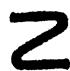
\includegraphics[keepaspectratio]{images/part002_cfff7d82.jpg}}

族 \((x_{i})\) 可和的这一必要条件一般绝不是充分的，即使 \(G\) 是完备的也是如此；后面我们会看到许多例子（见第四章，§ 7）。

推论. 设 \((x_{t})_{t\in I}\) 是交换群中的可和族，且该群的单位元有可数基本邻域系。那么指标 \(\iota\) 中使 \(x_{\iota}\neq 0\) 的那些组成的集合是可数的。

设 \((\mathbf{V}_{n})\) 是 0 的可数基本邻域系。若 \(\mathbf{H}_{n}\) 是使 \(x_{i} \notin \mathbf{V}_{n}\) 的所有指标 i 组成的集合，则使 \(x_{i} \neq 0\) 的指标 i 组成的集合 H 是诸集合 \(\mathbf{H}_{n}\) 的并，而由命题 1，每个 \(\mathbf{H}_{n}\) 都是有限的。

如果我们不假设原点有可数基本邻域系，这个推论就未必再成立。* 例如考虑积群 \(\mathbf{R}^{\mathbb{R}}\){[}实变量的所有有限实值函数作成的加法群，赋以逐点收敛拓扑（参看第十章，§ 1，第 3 节）{]}，并设 \(f_{a}\) 是 \(\mathbf{R}\) 中满足 \(f_{a}(a)=1\) 且 \(f_{a}(x)=0\)（当 \(x\neq a\) 时）的元素；那么族 \((f_{a})_{a\in\mathbb{R}}\) 是可和的，其和是在 \(\mathbf{R}\) 的每点取值都为 1 的函数。 *

注. 当 G 写作乘法时，Cauchy 判别准则取如下形式：为使族 \((x_{i})_{i\in I}\) 可乘，必须对单位元的每个邻域 V，存在 I 的有限子集 \(J_{0}\)，使得对 I 的每个不与 \(J_{0}\) 相交的有限子集 K，都有 \(\prod_{i\in K}x_{i}\in V\)；而且只要 G 是完备的，这个条件也是充分的。由此推出，若 I 是无限集且 \((x_{i})\) 可乘，则关于 I 的有限子集的余集所成的滤子，有 \(\lim x_{i}=1\)；若此外单位元还有可数基本邻域系，则使 \(x_{i}\neq1\) 的指标 i 组成的集合是可数的。

\subsection{部分和；结合性}

命题 2. 在完备群 G 中，可和族的每个子族都是可和的。

因为若族 \((x_{i})_{i\in I}\) 满足 Cauchy 判别准则，那么它的每个子族都平凡地满足该准则。

因此，若 \((x_{i})_{i\in I}\) 可和，则和 \(\sum_{i\in J}x_{i}\) 对每个子集 \(J\)（\(I\) 的，无论有限与否）都有定义：我们仍称它为族 \((x_{i})\) 的对应于指标集的子集 \(J\) 的部分和。可和族的部分和全体显然包含在有限部分和全体的闭包中。

定理 2（和的结合性）. 设 \((x_{i})_{i\in I}\) 是完备群 \(\mathbf{G}\) 中的可和族，并设 \((I_{\lambda})_{\lambda \in L}\) 是 \(\mathbf{I}\) 的任意一个分拆。若用 \(s_{\lambda}\) 表示 \(\sum_{i\in I_{\lambda}}x_{i}\)，则族 \((s_{\lambda})_{\lambda \in L}\) 可和且与族 \((x_{i})_{i\in I}\) 有相同的和。

设 \(s = \sum_{i \in I} x_i\)，并设 \(V\) 是 \(G\) 中 0 的任意闭邻域。那么存在有限子集 \(J_0\)（含于 \(I\)），使得对每个有限子集 \(J\)（含于 \(I\) 且包含 \(J_0\)），都有 \(\sum_{i \in J} x_i \in s + V\)。设 \(K_0\) 是 \(L\) 的由这样的指标 \(\lambda\) 组成的子集：它们使 \(J_\lambda = I_\lambda \cap J_0\) 非空；\(K_0\) 显然是有限的。设 \(K\) 是 \(L\) 的包含 \(K_0\) 的任意有限子集；我们将证明 \(\sum_{\lambda \in K} s_\lambda \in s + V\)，由此即证得定理。现在，\(s_\lambda\) 与 \((x_i)\) 的某个指标全属于 \(I_\lambda\) 的有限部分和非常接近；更精确地说，给定 0 的任意对称邻域 \(W\)，对每个 \(\lambda \in K\) 存在有限子集 \(H_\lambda\)（含于 \(I_\lambda\)，包含 \(J_\lambda\)），使得 \(s_\lambda - \sum_{i \in H_\lambda} x_i \in W\)。令 \(J = \bigcup_{\lambda \in K} H_\lambda\)；则 \(J\) 是 \(I\) 的包含 \(J_0\) 的有限子集，并且我们有

\[
\sum_ {i \in J} x _ {i} = \sum_ {\substack {i \in \bigcup_ {\lambda \in K} H _ {\lambda}}} x _ {i} = \sum_ {\lambda \in K} (\sum_ {i \in H _ {\lambda}} x _ {i})
\]

这是由有限和的结合性得到的。于是，由于 \(J_{0}\) 与诸 \(H_{\lambda}\) 的取法，我们有

\[
\sum_ {\lambda \in \mathbf {K}} s _ {\lambda} \in s + \mathbf {V} + n \mathbf {W}
\]

其中 \(n\) 是 \(\mathbf{K}\) 中元素的个数；这个关系式对每个 \(\mathbf{W}\) 都成立，从而也有 \(\sum_{\lambda \in \mathbb{K}} s_{\lambda} \in s + \mathbf{V}\)，因为 \(\mathbf{V}\)（是闭的）是诸邻域 \(\mathbf{V} + n\mathbf{W}\) 的交{[}§ 3，第 1 节，公式 (1){]}。

于是我们可以写出和的结合公式：

\[
\sum_ {\lambda \in L} (\sum_ {i \in I _ {\lambda}} x _ {i}) = \sum_ {i \in \bigcup_ {\lambda \in L} I _ {\lambda}} x _ {i},\tag{1}
\]

只要族 \((I_{\lambda})\) 是其并集的一个分拆且右端有定义，这个公式就成立。特别地，若指标集是积 \(I = L \times M\)，且“双重”族 \((x_{\lambda\mu})_{(\lambda,\mu) \in L \times M}\) 可和，我们就有求和次序交换的公式

\[
\sum_ {(\lambda , \mu) \in \mathbf {L} \times \mathbf {M}} x _ {\lambda \mu} = \sum_ {\lambda \in \mathbf {L}} (\sum_ {\mu \in \mathbf {M}} x _ {\lambda \mu}) = \sum_ {\mu \in \mathbf {M}} (\sum_ {\lambda \in \mathbf {L}} x _ {\lambda \mu}).\tag{2}
\]

应当指出，(1) 的左端可以有意义，而右端却没有定义。例如考虑 \(I = L \times \{1, 2\}\) 且 L 是无限集、\(I_{\lambda}\) 由 \((\lambda, 1)\) 与 \((\lambda, 2)\) 两个元素组成的情形；若取 \(x_{\lambda,1} = a\)，\(x_{\lambda,2} = -a\)，其中 \(a\) 是 \(\mathbf{G}\) 的任意非零元素，则对应于诸 \(I_{\lambda}\) 的所有部分和都为零，因此 (1) 的左端有定义且等于 0，而由命题 1，(1) 的右端没有意义。

同样可能发生这样的情形：(2) 的左端没有定义，但 (2) 中的两个“双重和”却都有意义；并且它们所表示的 G 的元素未必相等（见第四章，§ 7，习题 17）。

因此，虽然总是可以把一个和的项“结合”起来，但反过来却不可能把和式中本身表现为和的那些项“分解”为它们的元素。不过，只要这些“可分解”项的数目是有限的，这个运算就是合法的。

命题 3. 设 \((x_{\iota})_{\iota \in \mathbf{I}}\) 是群 \(\mathbf{G}\) 的点族，\((I_{\lambda})_{\lambda \in \mathbf{L}}\) 是 \(\mathbf{I}\) 的有限分拆。若每个子族 \((x_{\iota})_{\iota \in \mathbf{I}_{\lambda}}\) 都可和，则族 \((x_{\iota})_{\iota \in \mathbf{I}}\) 可和且公式 (1) 成立。

只需对 \(L = (1,2)\) 的情形证明本命题；在此基础上，再对 L 的元素个数用归纳法进行。设 \(s_{1} = \sum_{i \in I_{1}} x_{i}\)，\(s_{2} = \sum_{i \in I_{2}} x_{i}\)。对原点的每个邻域 V，存在有限子集 \(J_{1}\)（相应地，\(J_{2}\)），它含于 \(I_{1}\)（相应地，\(I_{2}\)），使得对每个有限子集 \(H_{1}\)（相应地，\(H_{2}\)）——含于 \(I_{1}\)（相应地，\(I_{2}\)）且包含 \(J_{1}\)（相应地，\(J_{2}\)）——有 \(\sum_{i \in H_{1}} x_{i} \in s_{1} + V\)（相应地，\(\sum_{i \in H_{2}} x_{i} \in s_{2} + V\)）。若令 \(J_{0} = J_{1} \cup J_{2}\)，则由此推出，对 I 的包含 \(J_{0}\) 的每个有限子集 H，有 \(\sum_{i \in H} x_{i} \in s_{1} + s_{2} + V + V\)，结论得证。

\subsection{群的积中的可和族}

命题 4. 设 \(G = \prod_{\lambda \in L} G_{\lambda}\) 是一族豪斯多夫交换群的积。那么诸点 \((x_{i})_{i \in I}\)（\(G\) 的点）构成的族可和当且仅当对每个 \(\lambda \in L\)，族 \((\mathbf{pr}_{\lambda} x_{i})_{i \in I}\) 可和；且若 \(s_{\lambda}\) 是这个族的和，则 \(s = (s_{\lambda})\) 是族 \((x_{i})\) 的和。

这由取值于积空间的函数关于滤子收敛的条件（第一章，§ 1，第 6 节，命题 10 的推论 1）立即得出；实际上，对 I 的每个有限子集 J，我们有

\[
\mathrm{pr} _ {\lambda} \left(\sum_ {i \in J} x _ {i}\right) = \sum_ {i \in J} \mathrm{pr} _ {\lambda} x _ {i}.
\]

\subsection{可和族在连续同态下的像}

命题 5. 设 \(f\) 是交换群 \(G\) 到交换群 \(G'\) 中的连续同态。若 \((x_t)\) 是 \(G\) 中的可和族，则 \((f(x_t))\) 是 \(G'\) 中的可和族，并且我们有

\[
\Sigma f (x _ {i}) = f (\Sigma x _ {i}).\tag{3}
\]

若 J 是指标集的任意有限子集，则 \(f\left(\sum_{i \in \mathbb{J}} x_i\right) = \sum_{i \in \mathbb{J}} f(x_i)\)，且收敛滤子基在 f 下的像是收敛滤子基（第一章，§ 7，第 4 节，命题 9 的推论 1）。

命题 6. 设 \((x_{i}), (y_{i})\) 是群 G 中有同一指标集的两个可和族。那么族 \((-x_{i}), (nx_{i})\)（ \(n \in \mathbf{Z}\)），\((x_{i} + y_{i})\) 都可和，并且我们有

\begin{enumerate}
\def\labelenumi{(\arabic{enumi})}
\setcounter{enumi}{3}
\tightlist
\item
\end{enumerate}

\[
\Sigma (- x _ {i}) = - \Sigma x _ {i},\tag{5}
\]

\[
\Sigma (n x _ {i}) = n \Sigma x _ {i},\tag{6}
\]

\[
\Sigma (x _ {i} + y _ {i}) = \Sigma x _ {i} + \Sigma y _ {i}.
\]

因为 \(x \rightarrow -x\) 与 \(x \rightarrow nx\) 都是 G 到 G 中的连续同态；另一方面，若 \((x_{t})\) 与 \((y_{t})\) 可和，则族 \((x_{t}, y_{t})\) 在 \(G \times G\) 中可和，且由于 \((x, y) \rightarrow x + y\) 是 \(G \times G\) 到 G 中的连续同态，我们即得 (6)。

注. 命题 4 与命题 5 也适用于前面提到过的情形，即具有一个结合且交换的合成法则的拓扑空间 X 中的可和族；若再假设 \(x + y\) 在 \(X \times X\) 上连续，则命题 3 与公式 (6) 也同样适用。

\subsection{级数}

考虑豪斯多夫交换群中的点列 \((x_{n})_{n\in \mathbb{N}}\)，并作部分和序列 \(s_n = \sum_{p=0}^{n} x_p (n \in \mathbb{N})\)。映射 \((x_{n}) \to (s_{n})\) 是集合 \(\mathbf{G}^{\mathbf{N}}\)（即点列 \((x_{n})\)（\(\mathbf{G}\) 中的）的全体）到其自身上的双射；因为若给定了序列 \((s_{n})\)，则序列 \((x_{n})\) 由关系 \(x_{0} = s_{0}, x_{n} = s_{n}-s_{n-1} (n \geqslant 1)\) 确定。

由序列 \((x_{n})\) 所定义的级数，或通项为 \(x_{n}\) 的级数{[}在不致混淆时，按用语之便，径称级数 \((x_{n})\){]}，定义为如上相关联的序列偶 \((x_{n})\) 与 \((s_{n})\)。由序列 \((x_{n})\) 所定义的级数称为收敛的，如果序列 \((s_n)\) 收敛；这个序列的极限称为级数的和，记作 \(\sum_{n=0}^{\infty} x_n\)（按记号之便，或记 \(\sum_{n=0}^{\infty} x_n\)）。

若通项为 \(x_{n}\) 的级数收敛，我们有时会按用语之便，称它为“级数 \(\sum_{n=0}^{\infty} x_{n}\)”或“级数 \(x_{0} + x_{1} + \cdots + x_{n} + \cdots\)”。

通项为 \(x_{n}\) 的级数收敛的一个必要条件是序列 \((s_{n})\) 为 Cauchy 序列，也就是说，对 G 中原点的每个邻域 V，存在整数 \(n_{0}\)，使得对每对整数 \(n \geqslant n_{0}, p > 0\)，有

\[
s _ {n + p} - s _ {n} = \sum_ {i = n + 1} ^ {n + p} x _ {i} \in V.
\]

若 \(\mathbf{G}\) 是完备的，这个条件也是充分的（级数的 Cauchy 判别准则）。

若通项为 \(x_{n}\) 的级数收敛，特别地我们有 \(\lim_{n\to \infty}(s_n - s_{n-1}) = \lim_{n\to \infty}x_n = 0\)；但这个收敛的必要条件一般绝不是充分的，即使 \(G\) 是完备的也是如此（见第四章，§ 7）。

命题 7. 若由序列 \((x_{n})\) 与 \((y_{n})\) 所定义的级数都收敛，则由序列 \((-x_{n})\) 与 \((x_{n} + y_{n})\) 所定义的级数也收敛，并且我们有

\[
\sum_ {n = 0} ^ {\infty} (- x _ {n}) = - \sum_ {n = 0} ^ {\infty} x _ {n},\tag{7}
\]

\[
\sum_ {n = 0} ^ {\infty} \left(x _ {n} + y _ {n}\right) = \sum_ {n = 0} ^ {\infty} x _ {n} + \sum_ {n = 0} ^ {\infty} y _ {n}.\tag{8}
\]

这是 \(-x\) 在 \(\mathbf{G}\) 上连续以及 \(x + y\) 在 \(\mathbf{G} \times \mathbf{G}\) 上连续的一个明显推论。

推论. 若 \((x_{n})\)、\((y_{n})\) 是 G 的两个点序列，使得除有限个指标外都有 \(x_{n}=y_{n}\)，且通项为 \(x_{n}\) 的级数收敛，则通项为 \(y_{n}\) 的级数也收敛。

因为通项为 \(x_{n} - y_{n}\) 的级数从某个指标起各项皆为零。

这个推论可以表述为：我们可以任意改动收敛级数的有限个项而不使它失去收敛性。特别地，若 \(y_{n} = 0\)（对 \(n < m\)），且 \(y_{n} = x_{n}\)（对 \(n \geqslant m\)），

则我们看到通项为 \(y_{n}\) 的级数收敛当且仅当通项为 \(x_{n}\) 的级数收敛；其和记作 \(\sum_{n=m}^{\infty} x_{n}\)，称为指标为 \(m\) 的余项（级数 \((x_{n})\) 的余项）。由于

\[
\sum_ {n = m} ^ {\infty} x _ {n} = \sum_ {n = 0} ^ {\infty} x _ {n} - s _ {m - 1},
\]

收敛级数的第 \(m\) 余项当 \(m\) 趋于 \(+\infty\) 时趋于 o。

若序列 \((x_{n})_{n\in I}\) 的指标集是 \(I\)——\(N\) 的无限子集——，且 \(\varphi\) 表示 \(N\) 到 \(I\) 上的保持严格序的双射，则按用语之便，称由序列 \((x_{\varphi(n)})_{n\in N}\) 所定义的级数为由序列 \((x_{n})_{n\in I}\) 所定义的级数；若这个级数收敛，其和记作 \(\sum_{n\in I}x_n\)。立即可以验证，这个级数收敛当且仅当通项为 \((z_n)\) 的级数收敛，其中 \(z_{n}=x_{n}\)（若 \(n\in I\)），而 \(z_{n}=0\)（若 \(n\in G I\)）。

\pandocbounded{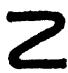
\includegraphics[keepaspectratio]{images/part002_ebf593f8.jpg}}

值得注意的是，若由序列 \((x_{n})_{n\in \mathbb{N}}\) 所定义的级数收敛，仍可能存在 \(\mathbf{N}\) 的无限子集 I，使得由子列 \((x_{n})_{n\in \mathbb{I}}\) 所定义的级数不收敛（见习题 5 及第四章，§ 7）。

命题 4 与命题 5 立即推广到级数，我们把它们在这一情形的表述留给读者。

命题 8（级数的受限结合性）. 设 \((k_n)\) 是一个严格递增的整数序列（\(\geqslant 0\)）。若通项为 \(x_n\) 的级数收敛，且令 \(u_n = \sum_{p=k_{n-1}}^{k_n-1} x_p\)，则通项为 \(u_n\) 的级数收敛，且我们有 \(\sum_{n=0}^{\infty} u_n = \sum_{n=0}^{\infty} x_n\)。

因为级数 \((u_{n})\) 的部分和序列是一个子列 \((s_{k_{n}-1})\)，它取自部分和序列 \((s_{n})\)（级数 \((x_{n})\) 的部分和序列）。

\subsection{交换收敛级数}

设 \((x_{n})\) 是 \(G\) 中的可和序列，并设 \(s = \sum_{n\in \mathbb{N}}x_n\) 是它的和。那么对每个邻域 \(V\)（\(0\) 的邻域），存在 \(J_0\in \mathfrak{F}(N)\)，使得 \(s_J\in s + V\) 只要 \(J\in \mathfrak{F}(N)\) 且 \(J_0\subset J\)。设 \(m\) 是 \(J_0\) 中最大的整数；则当 \(n\geqslant m\) 时有 \(s_n\in s + V\)，因而级数 \((x_{n})\) 收敛且其和为 \(s\)。但反之不成立：

收敛级数的项所成的序列完全可能不是可和的（见第四章，§ 7）。

此外，收敛级数的定义本质上涉及 N 的序结构。若级数 \((x_{n})\) 收敛，且 \(\sigma\) 是 N 的一个置换，则级数 \((x_{\sigma(n)})\) 未必收敛（参见第四章，§ 7，习题 15）。

定义 2. 由序列 \((x_{n})\) 所定义的级数称为交换收敛的，如果对每个置换 \(\sigma\)（\(\mathbf{N}\) 的置换），由序列 \((x_{\sigma(n)})\) 所定义的级数都收敛。

命题 9. 由序列 \((x_{n})\) 所定义的级数交换收敛当且仅当序列 \((x_{n})\) 可和；且此时对每个置换 \(\sigma\)（\(\mathbf{N}\) 的置换），我们有

\[
\sum_ {n = 0} ^ {\infty} x _ {\sigma} = \sum_ {n \in \mathbb {N}} x _ {n}.
\]

若序列可和，则级数显然交换收敛。为证反向的蕴含关系，我们用反证法，设级数 \((x_{n})\) 交换收敛而序列 \((x_{n})\) 不可和。于是滤子 \(\Phi\) 在映射 \(\mathbf{H} \to s_{\mathbf{H}}\) 下的像不能是 \(\mathbf{G}\) 中的 Cauchy 滤子基，否则这个滤子基将收敛，因为按假设它有一个聚点（第二章，§ 3，第 2 节，命题 5，推论 2）。因此存在一个邻域 \(\mathbf{V}\)（\(o\) 在 \(\mathbf{G}\) 中的一个邻域），使得对每个有限子集 \(\mathbf{J}\)（\(\mathbf{N}\) 的有限子集），存在有限子集 \(\mathbf{H}\)（\(\mathbf{N}\) 的有限子集），它不与 \(\mathbf{J}\) 相交，且使得 \(\sum_{n \in \mathbf{H}} x_{n} \notin V\)。于是，用归纳法，我们可以定义

把 N 分拆为有限子集 \(H_{k}\)（ \(k \in N\)），使得对无穷多个指标 k 有 \(\sum_{n \in H_{k}} x_{n} \notin V\)。显然存在 N 的一个置换 \(\sigma\)，使得对每个 k，使 \(\sigma(n) \in H_{k}\) 的那些 n 的值是相继的。若 \(\sigma\) 是这样一个置换，则通项为 \(x_{\sigma(n)}\) 的级数不可能收敛，于是得到矛盾。

若群 G 写作乘法，由 G 的点的序列 \((x_{n})\) 所定义的无穷乘积（或通项为 \(x_{n}\) 的无穷乘积，甚或在无混淆之虞时径称乘积 \(x_{n}\)）定义为序列 \((x_{n})\) 与部分积序列 \(p_{n}=\prod_{k=0}^{n}x_{k}\) 所构成的偶。若序列 \((p_{n})\) 收敛，则称该无穷乘积收敛，这个序列的极限记作 \(\prod_{n=0}^{\infty}x_{n}\)（按记号之便，或记 \(\prod_{n=0}^{\infty}x_{n}\)）。我们把将已建立的级数性质改写为乘法记号的任务留给读者。

\section{带算子拓扑群；拓扑环、除环与域}

\subsection{带算子拓扑群}

在集合 G 上，带算子的群结构与一个拓扑称为相容的，如果 G 的拓扑与群结构相容（§ 1，第 1 节），并且此外由算子所产生的 G 的自同态都是连续的。这时，集合 G 连同所给的拓扑与带算子的群结构，称为一个带算子拓扑群。

若 H 是带算子拓扑群 G 的稳定子群，则由 G 的拓扑在 H 上诱导的拓扑与 H 上的带算子群结构相容。此外：

命题 1. 若 H 是带算子拓扑群 G 的稳定子群，则 H 在 G 中的闭包 \(\overline{H}\) 是 G 的稳定子群。

我们已知（§ 2，第 1 节，命题 1）\(\overline{\mathbf{H}}\) 是 G 的子群。又若 \(\alpha\) 是 G 上的任一算子，则 H 在连续映射 \(x \to x^{\alpha}\) 下的像含于 H，因而 \(\overline{\mathbf{H}}\) 的像含于 \(\overline{\mathbf{H}}\)（第一章，§ 2，第 1 节，定理 1）。

设 H 是带算子拓扑群 G 的稳定正规子群。那么对 G 上的每个算子 \(\alpha\)，由 \(x \rightarrow x^{\alpha}\) 诱导的 G/H 到其自身的映射是连续的（§ 2，第 8 节，注 3），因此 G/H 上的带算子群结构与 G/H 上的商拓扑相容。

设 \((\mathbf{G}_i)_{i\in I}\) 是带算子拓扑群的一个族，其中假定每个 \(\mathbf{G}_i\) 有同一个算子集 \(\Omega\)。对每个 \(\alpha \in \Omega\)，映射 \(x\to ((\mathrm{pr}_i x)^{\alpha})\)（\(\mathbf{G} = \prod_{i\in I}\mathbf{G}_i\) 到其自身的映射）是连续的（第一章，§ 4，第 1 节，命题 1），因此 \(\mathbf{G}\) 上的带算子群结构与 \(\mathbf{G}\) 上的积拓扑相容。

若 G 是带算子的豪斯多夫拓扑群且 G 有完备化 \(\hat{G}\)（§ 3，第 4 节），则 G 上由算子定义的每个自同态 \(x \to x^{\alpha}\) 都可由连续性延拓为 \(\hat{\mathbf{G}}\) 的自同态（§ 3，第 3 节，命题 5）。于是 \(\hat{\mathbf{G}}\) 具有带算子拓扑群的结构，且 \(\hat{\mathbf{G}}\) 与 \(\mathbf{G}\) 有同一个算子集。

\subsection{稳定子群的拓扑直和}

由于带算子交换群的研究等同于模的研究，我们有时会容许自己对任意的带算子交换群使用专属于模的术语；这样，我们可以用线性映射一词来代替带算子交换群的同态，并可用投影算子一词来指带算子交换群的幂等自同态。

若带算子的交换拓扑群 \(\mathbf{E}\)（写作加法）是稳定子群的一个有限族 \((\mathbf{M}_i)_{1 \leqslant i \leqslant n}\) 的直和，则典范双射 \((x_i) \to \sum_{i=1}^{n} x_i\)（积群 \(\prod_{i=1}^{n} \mathbf{M}_i\) 到 \(\mathbf{E}\) 上的双射）是连续的，但未必是同胚。

定义 1. 设 E 是带算子的交换拓扑群，并设 \((\mathbf{M}_i)_{1 \leqslant i \leqslant n}\) 是 E 的稳定子群的一个有限族，使 E 是诸 \(\mathbf{M}_i\) 的直和。当下述条件成立时称 E 是诸 \(\mathbf{M}_i\) 的拓扑直和：典范映射 \((x_i) \to \sum_{i=1}^{n} x_i\)（积群 \(\prod_{i=1}^{n} \mathbf{M}_i\) 到 E 上的映射）是一个同胚（从而是带算子拓扑群的一个同构）。

命题 2. 设 E 是带算子的交换拓扑群，它是稳定子群 \(\mathbf{M}_i\)（ \(1 \leqslant i \leqslant n\)）的直和。设 \((p_i)_{1 \leqslant i \leqslant n}\) 是与分解 \(\mathbf{E} = \sum_{i=1}^{n} \mathbf{M}_i\) 相伴随的投影算子族。则 E 是诸 \(\mathbf{M}_i\) 的拓扑直和当且仅当诸 \(p_i\) 连续。

因为映射 \(x \to (p_i(x))\) 是映射 \((x_i) \to \sum_{i=1}^{n} x_i\) 的逆。

由于 \(\mathbf{I} = \sum_{i=1}^{n} p_i\)（其中 \(\mathbf{I}\) 表示 \(\mathbf{E}\) 的恒等映射），只需 \(n - \mathbf{I}\) 个投影算子 \(p_i\) 连续，便足以保证第 \(n\) 个也连续。

若 E 是两个稳定子群 M、N 的拓扑直和，则称 N 是 M 在 E 中的拓扑补；此事成立当且仅当 E/M 到 N 上的典范映射是带算子拓扑群的一个同构。

推论. 设 E 是带算子的交换拓扑群，并设 M 是 E 的稳定子群。那么下列条件等价：

\begin{enumerate}
\def\labelenumi{\alph{enumi})}
\item
  M 在 E 中有一个拓扑补。
\item
  存在连续投影算子 \(p\)（\(\mathbf{E}\) 到 \(\mathbf{E}\) 中的投影算子），使得 \(p(\mathbf{E}) = \mathbf{M}\)。
\item
  M 的恒等映射可以延拓为 E 到 M 上的一个连续线性映射。
\end{enumerate}

由命题 2 推出 a) 蕴含 b)，而 b) 蕴含 c) 是显然的。最后，若 p 是 E 到 M 上的一个连续线性映射，它延拓 M 的恒等映射，则 p 是一个连续投影算子，且投影算子 p 与 1-p 相伴于直和分解 \(E = M + N\)，其中 \(N = p^{-1}(\mathbf{o})\)。

注. 1) 为避免混淆，我们有时把 E 的作为 M 的补（就带算子群结构而言，不涉及拓扑）的稳定子群称为 M 的代数补。

\begin{enumerate}
\def\labelenumi{\arabic{enumi})}
\setcounter{enumi}{1}
\tightlist
\item
  若带算子的豪斯多夫交换拓扑群是稳定子群的一个族 \((\mathbf{M}_i)_{1\leqslant i\leqslant n}\) 的拓扑直和，则每个子群 \(\mathbf{M}_i\) 在 E 中闭，因为 \(\mathbf{M}_i\) 是由所有这样的 \(x\in E\) 组成的集合：它们满足 \(p_i(x) = x\)（第一章，§ 8，第 1 节，命题 2）。
\end{enumerate}

命题 3. 设 E、F 是两个带算子的交换拓扑群，并设 u 是 E 到 F 中的一个连续线性映射。为使存在 F 到 E 中的一个连续线性映射 v，使得 \(u \circ v\) 是 F 的恒等映射（这时称 u 为右可逆，称 v 为 u 的一个右逆），必须且只需 u 是 E 到 F 上的一个严格态射（§ 2，第 8 节），且 \(u^{-1}(\mathbf{o})\) 在 E 中有一个拓扑补。

这些条件是必要的。因为这时有 \(u(v(\mathbf{F})) = \mathbf{F}\)，并且 \(a\) fortiori（更有）\(u(\mathbf{E}) = \mathbf{F}\)；此外，若 \(p = v \circ u\)，则 \(p\) 是 \(\mathbf{E}\) 到其自身中的一个连续线性映射，满足 \(p^2 = p\)；因此（命题 2 的推论）\(p(\mathbf{E}) = v(u(\mathbf{E})) = v(\mathbf{F})\) 有一个拓扑补 \(p^{-1}(\mathbf{o})\)（在 \(\mathbf{E}\) 中的）；但按假设 \(u(p(x)) = u(x)\)，我们有 \(u^{-1}(\mathbf{o}) = p^{-1}(\mathbf{o})\)。最后，\(\mathrm{E}/p^{-1}(\mathbf{o})\) 到 \(\mathbf{F}\) 上的双射（与 \(u\) 相伴的双射），是如下两个映射的复合：\(\mathrm{E}/u^{-1}(\mathbf{o})\) 到 \(v(\mathbf{F})\) 上的双射（与 \(p\) 相伴的双射），以及 \(u\) 在 \(v(\mathbf{F})\) 上的限制；由于 \(v\) 连续，这两个映射都是同构，因此 \(u\) 是 \(\mathbf{E}\) 到 \(\mathbf{F}\) 上的一个严格态射。

这些条件是充分的。因为若 \(\varphi\) 是 E 到 \(\mathrm{E}/u^{-1}(\mathbf{o})\) 上的典范同态，则说 \(u^{-1}(\mathbf{o})\) 在 E 中有一个拓扑补 M，就等于说 \(\varphi\) 在 M 上的限制是 M 到 \(\mathrm{E}/u^{-1}(\mathbf{o})\) 上的一个同构。另一方面，由于 \(u=w\circ\varphi\)，其中 w 是 \(\mathrm{E}/u^{-1}(\mathbf{o})\) 到 F 上的一个同构，可见 u 在 M 上的限制是 M 到 F 上的一个同构，因而逆同构 v 使得 \(u\circ v\) 是 F 到其自身的恒等映射。

命题 4. 设 E、F 是两个带算子的交换拓扑群，并设 u 是 E 到 F 中的一个连续线性映射。为使存在 F 到 E 中的一个连续线性映射 v，使得 \(v \circ u\) 是 E 到其自身的恒等映射（这时称 u 为左可逆，称 v 为 u 的一个左逆），必须且只需 u 是 E 到 u(E) 上的一个（拓扑）同构，且 u(E) 在 F 中有一个拓扑补。

这些条件是充分的，因为若它们满足，就得到一个左逆 \(v\)（\(u\) 的左逆），其做法是把 \(u(\mathbf{E})\) 到 \(\mathbf{E}\) 上的同构（即 \(u\) 的逆）与 \(\mathbf{F}\) 到 \(u(\mathbf{E})\) 上的一个连续投影算子复合。

这些条件是必要的。因为关系 \(v(u(x)) = x\) 表明 \(u^{-1}(\mathbf{o}) = \{0\}\)；于是 \(u\) 是 \(E\) 到 \(u(E)\) 上的一个双射，且由于 \(v\) 在 \(u(E)\) 上的限制连续，由此得出 \(u\) 是 \(E\) 到 \(u(E)\) 上的一个同构。另一方面，若令 \(q = u \circ v\)，则 \(q\) 是 \(F\) 到 \(u(E)\) 上的一个连续线性映射，满足 \(q^2 = q\)，这就证明（命题 2 的推论）\(u(E)\) 在 \(F\) 中有一个拓扑补。

\subsection{拓扑环}

定义 2. 拓扑环是一个集合 A，其上带有环结构与一个拓扑，满足下列公理：

\((\mathrm{AT}_{\mathbf{I}})\). 映射 \((x,y) \to x + y\)（\(\mathbf{A} \times \mathbf{A}\) 到 \(\mathbf{A}\) 中的映射）是连续的。

\((\mathrm{AT}_{\mathbf{II}})\). 映射 \(x \to -x\)（A 到 A 中的映射）是连续的。

\((\mathrm{AT}_{\mathrm{III}})\). 映射 \((x,y)\to xy\)（\(\mathbf{A}\times \mathbf{A}\) 到 \(\mathbf{A}\) 中的映射）是连续的。

前两条公理表明 \(\mathbf{A}\) 的拓扑与其加法群结构相容（§ 1，第 1 节）。

若在集合 A 上给定了环结构与一个拓扑，则当它们满足公理 \((\mathrm{AT}_{\mathbf{I}})\)、\((\mathrm{AT}_{\mathbf{II}})\) 与 \((\mathrm{AT}_{\mathbf{III}})\) 时，称它们是相容的。

例. 1) 在任一环 A 上，离散拓扑与环结构相容。拓扑为离散的拓扑环称为离散环。

* 2) 我们将在第四章看到，有理直线 Q（相应地，实直线 R）的拓扑与 Q（相应地，R）的环结构相容。 *

在拓扑环中，每个左位似 \(x \rightarrow ax\)（相应地，每个右位似 \(x \rightarrow xa\)）都是连续的（且当 a 是 A 的单位时是同胚）。

由于我们可以恒等地写出

\[
x y - x _ {0} y _ {0} = (x - x _ {0}) (y - y _ {0}) + (x - x _ {0}) y _ {0} + x _ {0} (y - y _ {0})
\]

公理 \((\mathrm{AT}_{\mathrm{III}})\){[}结合 \((\mathrm{AT}_{\mathrm{I}})\) 与 \((\mathrm{AT}_{\mathrm{II}})\){]}就等价于下列两条公理的合取：

\((\mathrm{AT}_{\mathrm{III}a})\). 对任意 \(x_0\in \mathbf{A}\)，映射 \(x\to x_0x\) 与 \(x\rightarrow xx_0\) 在点 \(x = 0\) 连续

\((\mathrm{AT}_{\mathbf{III}\ b})\). 映射 \((x,y)\rightarrow xy\)（\(\mathbf{A}\times \mathbf{A}\) 到 A 中的映射）在点 (o, o) 连续。

由此我们可以导出一组充要条件，使滤子 \(\mathfrak{B}\)（\(o\) 在一个环 \(A\) 中的邻域滤子）必须满足它们，才能在 \(A\) 上定义一个与其环结构相容的拓扑：\(\mathfrak{B}\) 必须满足 § 1 的公理 \((\mathrm{GA}_{\mathrm{I}})\) 与 \((\mathrm{GA}_{\mathrm{II}})\)，并且还满足下列两条公理：

\((\mathrm{AV}_{1})\). 对所有 \(x_0\in \mathbf{A}\) 与所有 \(\mathbf{V}\in \mathfrak{B}\)，存在 \(\mathbf{W}\in \mathfrak{B}\)，使得 \(x_0\mathbf{W}\subset \mathbf{V}\) 且 \(\mathbf{W}x_0\subset \mathbf{V}\)

\((\mathrm{AV}_{\mathrm{II}})\). 对所有 \(\mathbf{V} \in \mathfrak{B}\)，存在 \(\mathbf{W} \in \mathfrak{B}\)，使得 \(\mathbf{WW} \subset \mathbf{V}\)。

注. 在分析中我们相当经常遇到满足公理 \((\mathrm{AT}_{\mathrm{I}})\)、\((\mathrm{AT}_{\mathrm{II}})\) 与 \((\mathrm{AT}_{\mathrm{III}a})\)，但不满足 \((\mathrm{AT}_{\mathrm{III}b})\) 的环。* 紧群上的测度环就是一个例子，其中乘法是卷积，拓扑是淡拓扑。 *

例 3). 设 \(\mathfrak{B}\) 是环 A 上的一个滤子基，由双边理想组成。\(\mathfrak{B}\) 是某个拓扑（与 A 的加法群结构相容的拓扑）的 o 的基本邻域系，且由 \((\mathrm{AV}_{\mathrm{I}})\) 与 \((\mathrm{AV}_{\mathrm{II}})\) 立即得出，这个拓扑与 A 的环结构相容。

设 X 是拓扑空间，f 与 g 是 X 到拓扑环 A 中的两个映射。若 f 与 g 在一点 \(x_{0} \in X\) 连续，则 \(f + g\)、-f 与 fg 在该点连续。由此得出，X 到 A 中的连续映射组成 X 到 A 的一切映射所成之环 \(A^{X}\) 的一个子环。我们还看到，若 A 交换，则每个 n 个变元、系数在 A 中且定义在 \(A^{n}\) 上的多项式都在 \(A^{n}\) 上连续。再者，设 f 与 g 是一个集合 X（由滤子 F 所滤化）到豪斯多夫拓扑环 A 中的两个映射；若 \(\lim_{\mathfrak{F}} f\) 与 \(\lim_{\mathfrak{F}} g\) 存在，则 \(\lim_{\mathfrak{F}} (f + g)\)、\(\lim_{\mathfrak{F}} (-f)\) 与 \(\lim_{\mathfrak{F}} (fg)\) 也存在，并且我们有（第一章，§7，第 4 节，命题 9，推论 1，及 §8，第 1 节，命题 1）

\[
\lim _ {\mathfrak {F}} (f + g) = \lim _ {\mathfrak {F}} f + \lim _ {\mathfrak {F}} g,\tag{1}
\]

\[
\lim _ {\mathfrak {F}} (- f) = - \lim _ {\mathfrak {F}} f,\tag{2}
\]

\[
\lim _ {\mathfrak {F}} (f g) = (\lim _ {\mathfrak {F}} f) (\lim _ {\mathfrak {F}} g).\tag{3}
\]

\subsection{子环；理想；商环；环的积}

若 H 是拓扑环 A 的子环，则由 A 的拓扑在 H 上诱导的拓扑与 H 的环结构相容。这样在 H 上定义的拓扑环结构称为由 A 的拓扑环结构所诱导。

命题 5. 设 H 是拓扑环 A 的稠密子环，并设 K 是 H 的子环（相应地，左理想、右理想、双边理想）。则 K 在 A 中的闭包 K 是 A 的子环（相应地，左理想、右理想、双边理想）。

证明与 § 2 第 3 节命题 8 的证明相同：例如若 K 是 H 中的左理想，则映射 \((z, x) \to zx\) 在 \(A \times A\) 上连续，且把 \(H \times K\) 映入 K；因而它把 \(A \times K = \overline{H} \times K\) 映入 \(\overline{H}\)。

设 H 是拓扑环 A 中的双边理想。用与商群情形同样的论证，我们看到 A 的拓扑由关系 \(x - y \in H\) 作出的商与 A/H 的环结构相容。特别地，若 A 不是豪斯多夫的，则 \(\{o\}\) 在 A 中的闭包 N 由命题 5 是一个闭双边理想；商环是豪斯多夫的（§ 2，第 5 节，命题 13），称为与 A 相伴的 Hausdorff 环。

设 \((\mathbf{A}_t)_{t\in \mathbf{I}}\) 是拓扑环的一个族。在集合 \(\mathbf{A} = \prod_{t\in \mathbf{I}}\mathbf{A}_t\) 上，诸 \(\mathbf{A}_t\) 的拓扑之积与诸 \(\mathbf{A}_t\) 的环结构之积相容（与积群情形的证明相同）；这样定义的拓扑环 \(\mathbf{A}\) 称为诸拓扑环 \(\mathbf{A}_t\) 的积。

\subsection{拓扑环的完备化}

当我们说到拓扑环的一致结构时，除非另有明确说明，我们总是指其加法群的一致结构；特别地，若 A 的加法群完备，则称 A 为完备环。

设 A 是豪斯多夫拓扑环；作为加法群，A 可以看作完备豪斯多夫交换群 \(\hat{\mathbf{A}}\) 的一个稠密子群，后者在相差一个同构的意义下被确定（§ 3，第 5 节，定理 2）。为使我们可以把 A 看作完备环的子环，必须能够把函数 \(xy\) 由连续性延拓到空间 \(\hat{\mathbf{A}} \times \hat{\mathbf{A}}\) 上。这种延拓的可能性将由下面更一般的定理得出：

定理 1. 设 E、F、G 是三个完备豪斯多夫交换群；设 A 是 E 的稠密子群，B 是 F 的稠密子群。若 f 是 A × B 到 G 中的一个连续 Z-双线性（*）映射，则 f 可由连续性延拓为 E × F 到 G 中的一个连续 Z-双线性映射。

设 \((x_{0}, y_{0})\) 是 \(E \times F\) 的任意一点，并设 \(\mathfrak{U}\)、\(\mathfrak{B}\) 分别是 \(x_{0}, y_{0}\) 的邻域滤子在 A、B 上的迹（按假设 \(\mathfrak{U}\)、\(\mathfrak{B}\) 是滤子）。为证 f 可由连续性延拓，只需证明 \(f(\mathfrak{U} \times \mathfrak{V})\) 是 G 上的一个 Cauchy 滤子基（第二章，§ 3，第 6 节，命题 11）。考虑恒等式

\[
f \left(x ^ {\prime}, y ^ {\prime}\right) - f (x, y) = f \left(x ^ {\prime} - x, y _ {1}\right) + f \left(x _ {1}, y ^ {\prime} - y\right) + f \left(x ^ {\prime} - x, y ^ {\prime} - y _ {1}\right).
\]

我们将证明，取 \((x, y)\) 与 \((x', y')\) 属于 \(\mathfrak{U} \times \mathfrak{B}\) 的一个充分小的集合，并适当选取 \(x_{1}\) 与 \(y_{1}\)，就可以使右端各项都很小。设 W 是 G 中 o 的任一邻域；由于 f 在 \((o, o) \in A \times B\) 连续，存在集合 \(U \in \mathfrak{U}\) 与集合 \(V \in \mathfrak{B}\)，使得 \(f(x' - x, y' - y) \in W\) 对 \(x \in U\)、\(x' \in U\)、\(y \in V\)、\(y' \in V\) 均成立。取一点 \(x_{1} \in U\) 与一点 \(y_{1} \in V\)；则对 U 中所有 \(x, x'\) 与 V 中所有 \(y, y'\)，我们将有

\[
f \left(x ^ {\prime} - x, y ^ {\prime} - y _ {1}\right) + f \left(x - x _ {1}, y ^ {\prime} - y\right) \in \mathrm{W} + \mathrm{W}.
\]

另一方面，偏映射 \(x \to f(x, y_1)\) 在 A 上连续；因而存在集合 \(U' \subset U\)（属于 \(\mathfrak{U}\)），使得只要 \(x\) 与 \(x'\) 属于 \(U'\)，就有 \(f(x' - x, y_1) \in W\)。同样，存在 \(V' \subset V\)（属于 \(\mathfrak{B}\)），使得只要 \(y\) 与 \(y'\) 属于 \(V'\)，就有 \(f(x_1, y' - y) \in W\)。于是，若 \((x, y)\) 与 \((x', y')\) 是 \(U' \times V'\) 的任意两点，则

\[
f \left(x ^ {\prime}, y ^ {\prime}\right) - f (x, y) \in W + W + W + W;
\]

这就证明了延拓 \(\overline{f}\)（\(f\) 的延拓）的存在性。\(\overline{f}\) 是 \(\mathbf{Z}\)-双线性的这一事实，是恒等延拓原理（第一章，§ 8，第 1 节，命题 2 的推论 1）的直接推论。

证毕。

在把这一定理应用于豪斯多夫拓扑环 A 时，我们取 E、F 与 G 为 \(\hat{A}\)，取 A 与 B 为环 A，并取 f 为 Z-双线性映射 \((x, y) \to xy\)，按假设它是连续的。我们仍用 xy 表示延拓后的函数在 \(\hat{A} \times \hat{A}\) 上的值；这个函数是 \(\hat{A}\) 上的一个合成法则，说它是 Z-双线性的，就是说它关于加法双侧分配；又由恒等延拓原理，它也是结合的。于是：

命题 6. 豪斯多夫拓扑环 A 同构于完备豪斯多夫环 \(\hat{\mathbf{A}}\) 的一个稠密子环，后者在相差一个同构的意义下被确定（并称为 A 的完备化）。

若 A 交换（相应地，有单位元），则 \(\hat{A}\) 亦然（恒等延拓原理）。

设 A 是拓扑环，不必是豪斯多夫的；设 N 是 \(\{o\}\) 在 A 中的闭包，并设 \(A' = A/N\) 是与 A 相伴的 Hausdorff 环。则 \(\hat{A}'\)——\(A'\) 的完备化——称为 A 的 Hausdorff 完备化，也记作 \(\hat{A}\)。与 §3 第 4 节命题 8 一样可以证明，A 到完备豪斯多夫拓扑环 C 中的每个连续环同态 u 都可以唯一分解为 \(u = v \circ \varphi\)，其中 v 是 \(\hat{A}\) 到 C 中的连续同态，而 \(\varphi\) 是 A 到 \(\hat{A}\) 中的典范映射。若 A、B 是两个拓扑环，且 \(u : A \to B\) 是连续同态，则存在唯一的连续同态 \(\hat{u} : \hat{A} \to \hat{B}\)，使得图表

\[
\begin{array}{c c c} \mathbf {A} & \stackrel {{u}} {{\longrightarrow}} & \mathbf {B} \\ \varphi \Big \downarrow & & \Big \downarrow \psi \\ \hat {\mathbf {A}} & \stackrel {{\hat {u}}} {{\longrightarrow}} & \hat {\mathbf {B}} \end{array}
\]

是交换的（ \(\varphi\) 与 \(\psi\) 是典范映射）；只需对 \(\psi \circ u\) 应用前面的结果。

\subsection{拓扑模}

定义 3. 给定一个有单位元的拓扑环 A，拓扑左 A-模是一个集合 E，连同：

\begin{enumerate}
\def\labelenumi{\arabic{enumi})}
\item
  一个左 A-模结构；
\item
  一个与 E 的加法群结构相容的拓扑，且满足下列公理：
\end{enumerate}

(MT) 映射 \((\lambda, x) \to \lambda x\)（\(\mathbf{A} \times \mathbf{E}\) 到 \(\mathbf{E}\) 中的映射）是连续的。

我们类似地定义拓扑右 A-模的概念；由于每个右 A-模都可以看作左 A°-模（其中 A° 是 A 的反环），且 A 的拓扑与 A° 的环结构相容，因此无须区分拓扑右 A-模与拓扑左 A°-模。

例. *1) R（相应地，C）上的拓扑向量空间是拓扑 R（相应地，C）模。

\begin{enumerate}
\def\labelenumi{\arabic{enumi})}
\setcounter{enumi}{1}
\tightlist
\item
  设 A 是环，B 是 A 上由 A 的双边理想组成的一个滤子基；设 E 是左 A-模。若给 A 赋以 B 为 o 的基本邻域系的拓扑（与其环结构相容的拓扑）（第 3 节，例 3），并给 E 赋以诸集合 aE（当 a 取遍 B 时）构成 o 的基本邻域系的拓扑（与其加法群结构相容）（§ 1，第 2 节，例），则立即可以验证 E 是拓扑 A-模。
\end{enumerate}

注. 给定拓扑环 A，在左 A-模 E 上考虑一个与 E 的加法群结构相容的拓扑。凭恒等式

\[
\lambda x - \lambda_ {0} x _ {0} = (\lambda - \lambda_ {0}) x _ {0} + \lambda_ {0} (x - x _ {0}) + (\lambda - \lambda_ {0}) (x - x _ {0})
\]

公理 (MT) 等价于下列三条公理的合取：

\((\mathbf{MT}_{\mathbf{I}}^{\prime})\). 对每个 \(x_0\in \mathbf{E}\)，映射 \(\lambda \to \lambda x_0\) 在点 \(\lambda = 0\) 连续

\((\mathbf{MT}_{\mathrm{II}}^{\prime})\). 对每个 \(\lambda_0\in \mathbf{A}\)，映射 \(x\to \lambda_0x\) 在点 \(x = 0\) 连续

\((\mathbf{MT}_{\mathrm{III}}^{\prime})\). 映射 \((\lambda ,x)\to \lambda x\) 在点 (o, o) 连续。

由此我们导出一组充要条件，A-模 E 中 o 的邻域滤子 \(\mathfrak{B}\) 必须满足它们，才能在 E 上定义一个与其模结构相容的拓扑；\(\mathfrak{B}\) 必须满足 § 1 第 2 节的公理 (GA \(_{\mathrm{I}}\) ) 与 (GA \(_{\mathrm{II}}\) )，此外还必须满足下列三条公理：

\((\mathbf{MV}_{\mathrm{I}})\). 对每个 \(x_0 \in E\) 与 V \(\in \mathfrak{B}\)，存在 A 中 o 的一个邻域 S，使得 S. \(x_0 \subset V\)。

\((\mathbf{MV}_{\mathrm{II}})\). 对每个 \(\lambda_0 \in \mathbf{A}\) 与 \(V \in \mathfrak{B}\)，存在 \(W \in \mathfrak{B}\)，使得 \(\lambda_0 W \subset V\)。\((\mathbf{MV}_{\mathrm{III}})\). 对每个 \(V \in \mathfrak{B}\)，存在 \(U \in \mathfrak{B}\) 与一个邻域 \(T\)（\(o\) 在 \(A\) 中的一个邻域），使得 \(T. U \subset V\)。

当环 \(\mathbf{Z}\) 赋以离散拓扑时，每个交换拓扑群都是拓扑 \(\mathbf{Z}\)-模。

若 M 是拓扑 A-模 E 的子模，则显然由 E 的拓扑在 M 上诱导的拓扑与 M 的模结构相容。此外，在商 A-模 E/M 上，E 的拓扑对 M 作出的商拓扑与 A-模结构相容。为看清这一点，只需证明映射 \((\lambda, \dot{x}) \to \lambda \dot{x}\)（\(\mathbf{A} \times (\mathbf{E} / \mathbf{M})\) 到 \(\mathbf{E} / \mathbf{M}\) 上的映射）连续（其中 \(x \to \dot{x}\) 表示 \(\mathbf{E}\) 到 \(\mathbf{E} / \mathbf{M}\) 上的典范映射）。现在，由于我们可以把加法拓扑群 \(\mathbf{A} \times (\mathbf{E} / \mathbf{M})\) 与 \((\mathbf{A} \times \mathbf{E}) / (\{\mathbf{o}\} \times \mathbf{M})\) 等同起来（§ 2，第 9 节，命题 26 的推论），只需证明映射 \((\lambda, x) \to \lambda \dot{x}\)（\(\mathbf{A} \times \mathbf{E}\) 到 \(\mathbf{E} / \mathbf{M}\) 中的映射）连续；而这是直接的，因为所论映射是 \(x \to \dot{x}\) 与 \((\lambda, x) \to \lambda x\) 的复合。

设 \((\mathbf{E}_i)_{i\in \mathbf{I}}\) 是拓扑 A-模的任意一个族，并设 \(\mathbf{E} = \prod_{i\in \mathbf{I}}\mathbf{E}_i\) 是诸 \(\mathbf{E}_i\) 之积这个 A-模。则 E 上的

积拓扑与 E 的 A-模结构相容。为证明这一点，只需证明 A × E 到 E 中的映射 \((\lambda, x) \to (\lambda \cdot \text{pr}_i x)_{i \in I}\) 连续，或者（由第一章 § 4 第 1 节命题 1）对每个指标 \(i \in I\)，映射 \((\lambda, x) \to \lambda \cdot \text{pr}_i x\) 是 A × E 到 \(E_i\) 中的连续映射；但这个映射是 \((\lambda, x_i) \to \lambda x_i\) 与 \((\lambda, x) \to (\lambda, \text{pr}_i x)\) 的复合，而这两个映射都是连续的。

设 A 是豪斯多夫拓扑环，E 是豪斯多夫拓扑 A-模。设 \(\hat{\mathbf{E}}\) 是作为交换拓扑群 E 的完备化的那个加法群（§ 3，第 5 节，定理 2）。Z-双线性映射 \((\lambda, x) \to \lambda x\)（加法群 A、E 之积 \(\mathbf{A} \times \mathbf{E}\) 到加法群 E 中的映射）可由连续性延拓为 \(\hat{\mathbf{A}} \times \hat{\mathbf{E}}\) 到 \(\hat{\mathbf{E}}\) 中的 Z-双线性映射（第 5 节，定理 1），我们仍把这个映射记作 \((\lambda, x) \to \lambda x\)。由恒等延拓原理，我们有 \(\lambda(\mu x) = (\lambda \mu)x\)（对 \(\lambda \in \hat{\mathbf{A}}\)、\(\mu \in \hat{\mathbf{A}}\) 与 \(x \in \hat{\mathbf{E}}\)），且 \(1.x = x\) 对所有 \(x \in \hat{\mathbf{E}}\)；因此外合成法则 \((\lambda, x) \to \lambda x\) 所定义的 \(\hat{\mathbf{A}}\)-模结构在 \(\hat{\mathbf{E}}\) 上与它的拓扑相容。这样定义的拓扑 \(\hat{\mathbf{A}}\)-模 \(\hat{\mathbf{E}}\) 称为拓扑 A-模 E 的完备化。

设 E 是拓扑环 A 上的拓扑模，其中 A 与 E 都不必是豪斯多夫的。设 N（相应地，F）是 \(\{o\}\) 在 A（相应地，E）中的闭包。N 是 A 的双边理想（第 4 节，命题 5），F 是 E 的子 A-模（第 1 节，命题 1）；此外，由连续性我们有 \(\lambda x \in F\)，只要 \(\lambda \in N\) 或 \(x \in F\)。因此我们可以通过过渡到商来定义映射 \((\dot{\lambda}, \dot{x}) \to \dot{\lambda} \dot{x}\)（\((A/N) \times (E/F)\) 到 E/F 中的映射）；容易验证（利用 § 2 第 9 节命题 26 的推论）这个映射连续，从而在 E/F 上定义了一个拓扑 \((A/N)\)-模结构。若令 B = A/N 与 L = E/F，则 B-模 L 称为与 E 相伴的 Hausdorff 模；它的完备化 \(\hat{L}\) 是 \(\hat{A}\)——A 的 Hausdorff 完备化，按定义等于 \(\hat{B}\)——上的一个拓扑模（第 5 节），而这个模 \(\hat{L}\) 称为 E 的 Hausdorff 完备化，记作

\(\hat{\mathbf{E}}\)。与 § 3 第 4 节命题 8 一样可以看到，每个连续同态 \(u: \mathbf{E} \to \mathbf{G}\)（\(\mathbf{E}\) 到完备豪斯多夫 \(\hat{\mathbf{A}}\)-模 \(\mathbf{G}\) 中的连续同态）都唯一分解为 \(u = v \circ \varphi\)，其中 \(v\) 是 \(\hat{\mathbf{E}}\) 到 \(\mathbf{G}\) 中的连续同态，而 \(\varphi\) 是 \(\mathbf{E}\) 到 \(\hat{\mathbf{E}}\) 中的典范映射。我们断言，若 \(\mathbf{E}, \mathbf{E}'\) 是两个拓扑 A-模，且 \(u: \mathbf{E} \to \mathbf{E}'\) 是连续同态，则存在唯一的连续同态 \(\hat{u}: \hat{\mathbf{E}} \to \hat{\mathbf{E}}'\)，使得图表

\[
\begin{array}{c c c} \mathbf {E} & \stackrel {{u}} {{\longrightarrow}} & \mathbf {E} ^ {\prime} \\ \varphi \Big \downarrow & & \Big \downarrow \varphi^ {\prime} \\ \hat {\mathbf {E}} & \stackrel {{\hat {u}}} {{\longrightarrow}} & \hat {\mathbf {E}} ^ {\prime} \end{array}
\]

是交换的，其中 \(\varphi\) 与 \(\varphi'\) 是典范映射。

本节的定义与结果同样适用于任意拓扑环上的伪模，只需删去所有关于环的单位元的提述。

\subsection{拓扑除环与域}

在下文以及第四、第五章中，若 K 是一个除环，我们用 \(K^{*}\) 表示 K 的非零元素所成的乘法群。

定义 4. 拓扑除环是一个集合 K，其上带有除环结构与一个和 K 的环结构相容的拓扑，且此外还满足下列公理：

(KT) 映射 \(x \to x^{-1}\)（\(\mathbf{K}^*\) 到 \(\mathbf{K}^*\) 中的映射）是连续的。

交换的拓扑除环称为拓扑域。

集合 K 上的除环结构与一个拓扑称为相容的，如果相应的环结构与该拓扑相容，且此外公理 (KT) 成立。

例. 1) 在任一除环 K 上，离散拓扑与除环结构相容。拓扑为离散的拓扑除环称为离散除环。

* 2) 有理直线 Q（相应地，实直线 R）的拓扑与 R（相应地，R）的域结构相容（见第四章，§ 3）。*

定义 4 表明，若 K 是拓扑除环，则由 K 的拓扑在乘法群 \(K^{*}\) 上诱导的拓扑与 \(K^{*}\) 的群结构相容。

若 \(a \neq 0\)，则位似 \(x \rightarrow ax\) 与 \(x \rightarrow xa\) 都是 K 到其自身上的同胚；且映射 \(x \rightarrow ax + b\) 对所有 \(b \in K\) 亦然。注意，位似 \(x \rightarrow ax\) 与 \(x \rightarrow xa\) 在 \(a \neq 0\) 时是 K 的（拓扑）加法群的自同构。由此，若 V 是 K 中 o 的任一邻域，则对所有 \(a \neq 0\)，aV 与 Va 都是 o 的邻域。

设 X 是拓扑空间，f 是 X 到拓扑除环 K 中的一个映射。若 f 在一点 \(x_{0} \in X\) 连续且 \(f(x_{0}) \neq 0\)，则 \(f^{-1}\) 在 \(x_{0}\) 连续。特别地，若 K 是拓扑域，则每个 n 个变元、系数在 K 中的有理函数，都在 \(K^{n}\) 上其分母不为零的每一点连续。

同样，若 \(f\) 是一个集合 \(\mathbf{X}\)（由滤子 \(\mathfrak{F}\) 所滤化）到豪斯多夫拓扑除环 \(\mathbf{K}\) 中的映射，且 \(\lim_{\mathfrak{F}} f\) 存在且不为 \(o\)，则 \(\lim_{\mathfrak{F}} f^{-1}\) 存在，并且我们有

\[
\lim _ {\mathfrak {F}} f ^ {- 1} = (\lim _ {\mathfrak {F}} f) ^ {- 1}.\tag{4}
\]

若 H 是拓扑除环 K 的除子环，则由 K 的拓扑在 H 上诱导的拓扑与 H 的除环结构相容。这样在 H 上定义的拓扑除环结构称为由 K 的拓扑除环结构所诱导。此外，\(\overline{H}\) 也是 K 的除子环（证明与命题 5 的证明类似）。

在拓扑除环 K 中，集合 \(\{0\}\) 的闭包由命题 5 是一个双边理想，因而必须是 \(\{0\}\) 或 K。换句话说，若 K 的拓扑不是最粗拓扑（第一章，§ 2，第 2 节），则它是豪斯多夫的（§ 1，第 2 节，命题 2）。

\subsection{拓扑除环上的一致结构}

若 K 是拓扑除环，就必须区分：1) K 的加法群的一致结构，它定义在 K 上，称为 K 的加法一致结构；与 2) 乘法群 \(\mathbf{K}^*\) 的左一致结构与右一致结构，它们定义在 \(\mathbf{K}^*\) 上，并（按用语之便）称为 K 的乘法一致结构。

由 K 的加法一致结构在 \(K^{*}\) 上诱导的一致结构一般不同于 K 的乘法一致结构（见习题 17）。

由命题 6，豪斯多夫拓扑除环 K 可以看作完备豪斯多夫环 \(\hat{K}\) 的一个稠密子环。为使 \(\hat{K}\) 是拓扑除环，必须映射 \(x \to x^{-1}\) 可由连续性延拓到 \((\hat{\mathbf{K}})^{*}\) 上；而这个必要条件也是充分的，因为这时函数 \(xx^{-1}, x^{-1}x\) 与 \(1\) 由恒等延拓原理在 \((\hat{\mathbf{K}})^{*}\) 上相等，因此延拓后的函数的值是 \(x\) 的逆，这里 \(x \neq 0\) 取遍 \(\hat{\mathbf{K}}\)。换句话说（参见第二章，§ 3，第 6 节，命题 11）：

命题 7. 完备化 \(\hat{\mathbf{K}}\)——豪斯多夫拓扑除环 \(\mathbf{K}\) 的完备化——是拓扑除环，当且仅当在映射 \(x \to x^{-1}\) 下，每个不以 0 为聚点的（关于加法结构的）Cauchy 滤子的像，都是（关于加法结构的）Cauchy 滤子。

\pandocbounded{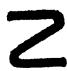
\includegraphics[keepaspectratio]{images/part002_56877e98.jpg}}

存在这样的拓扑除环，其中这一条件不满足，且其中环 \(\hat{\mathbf{K}}\) 有零因子（见习题 26）。此外，即使完备化 \(\hat{\mathbf{K}}\) 是拓扑除环，也没有先验的理由认为 \(\hat{\mathbf{K}}\) 的乘法一致结构是完备空间的结构。然而，对于除环 \(\mathbf{K}\)——只要 \(\hat{\mathbf{K}}\) 局部紧（见第一章，§ 9，第 7 节，命题 13，及第三章，§ 3，第 3 节，命题 4）——以及对于拓扑域，情形就是如此；对后者，我们有下列命题：

命题 8. 若拓扑域 K 的加法一致结构是完备豪斯多夫空间的结构，则 \(K^{*}\) 上的乘法一致结构是完备空间的结构。

我们将证明，若 \(\mathfrak{F}\) 是 \(\mathbf{K}^*\) 上关于乘法一致结构的 Cauchy 滤子，则 \(\mathfrak{F}\) 是 \(\mathbf{K}\) 上关于加法一致结构的 Cauchy 滤子，且不收敛于 \(o\)；这样就证得了结果。设 \(\mathbf{U}\) 是 \(o\) 在 \(\mathbf{K}\) 中的一个任意邻域，设 \(\mathbf{V}\) 是 \(o\) 的闭邻域，使得 \(\mathbf{V} \subset \mathbf{U}\)、\(\mathbf{VV} \subset \mathbf{U}\){[}公理 \((\mathrm{AV}_{\mathrm{II}})]\) 且 \(-1 \notin V\)；则按假设存在集合 \(\mathbf{A} \in \mathfrak{F}\)，使得对所有 \(x \in \mathbf{A}\) 与 \(y \in \mathbf{A}\)，有 \(x^{-1}y \in 1 + V\)。取 \(a \in \mathbf{A}\)，则 \(\mathbf{A} \subset a + aV\)，而 \(a + aV\) 是不含 \(o\) 的闭集；因此 \(o\) 不在 \(\mathbf{A}\) 的闭包中，从而不是 \(\mathfrak{F}\) 的聚点。设 \(\mathbf{W}\) 是 \(o\) 的邻域，使得 \(aW \subset V\){[}公理 \((\mathrm{AV}_{\mathrm{I}})]\)；则按假设存在集合 \(\mathbf{B} \in \mathfrak{F}\)，使得 \(\mathbf{B} \subset \mathbf{A}\)，且对所有 \(x \in B\) 与 \(y \in B\)，有 \(x^{-1}y \in 1 + W\)；于是 \(y - x \in xW \subset AW \subset aW + aVW\)；但 \(\mathbf{K}\) 交换，因此 \(aVW = aWV \subset VV \subset U\)；从而 \(y - x \in U + U\)，命题得证。

同样的证明表明，命题 8 可以推广到如下的情形：关于 K 的两个乘法一致结构之一的每个 Cauchy 滤子，也是关于另一个乘法一致结构的 Cauchy 滤子。

\section{拓扑群与拓扑环的逆极限}

在本节中，I 表示一个非空有向集（*），而 \(\alpha \leqslant \beta\) 表示 I 中的偏序关系。除非另有明确说明，所考虑的一切逆系统都以 I 为指标。
% semantic-fragments: legacy-input-seam
\relax{}
\subsection{代数结构的逆极限}

设 \((\mathbf{X}_{\alpha}, f_{\alpha\beta})\) 是集合的一个逆系统，并设每个 \(X_{\alpha}\) 赋有一个内合成法则，它处处有定义，且写成乘法形式。再设诸 \(f_{\alpha\beta}\) 是关于这些内合成法则的同态。由于

\[
f _ {\alpha \beta} (x _ {\beta}. y _ {\beta}) = f _ {\alpha \beta} (x _ {\beta}). f _ {\alpha \beta} (y _ {\beta})
\]

只要 \(\alpha \leqslant \beta\) 且 \(x_{\beta}\) 与 \(y_{\beta}\) 属于 \(\mathbf{X}_{\beta}\) ，显然 \(\mathbf{X} = \varprojlim \mathbf{X}_{\alpha}\) 是乘积 \(\prod_{\alpha} \mathbf{X}_{\alpha}\) 关于内合成法则 \((x_{\alpha}) \cdot (y_{\alpha}) = (x_{\alpha} \cdot y_{\alpha})\) 的一个稳定子集。设 \((\Lambda_{\alpha}, \varphi_{\alpha\beta})\) 是另一个以 I 为指标集的集合逆系统，并设每个 \(\mathbf{X}_{\alpha}\) 载有一个外合成法则，它处处有定义、写成乘法形式且以 \(\Lambda_{\alpha}\) 为算子集，使得只要 \(\alpha \leqslant \beta\) 就有

\[
f _ {\alpha \beta} (\lambda_ {\beta}. x _ {\beta}) = \varphi_ {\alpha \beta} (\lambda_ {\beta}). f _ {\alpha \beta} (x _ {\beta})
\]

对 \(\lambda_{\beta} \in \Lambda_{\beta}\) 与 \(x_{\beta} \in X_{\beta}\) 成立。于是我们可以在 \(\prod_{\alpha} X_{\alpha}\) 上定义一个外法则，它以 \(\prod_{\alpha} \Lambda_{\alpha}\) 为算子集，定义方式为 \((\lambda_{\alpha}) \cdot (x_{\alpha}) = (\lambda_{\alpha} \cdot x_{\alpha})\) ；把算子集限制为 \(\Lambda = \varprojlim \Lambda_{\alpha}\) ，便得到 \(\prod_{\alpha} X_{\alpha}\) 上的一个外法则，\(X\) 关于它仍是一个稳定子集。这样定义在 X 上的内

（相应地，外）法则称为诸 \(X_{\alpha}\) 的内（相应地，外）法则的逆极限。就外法则而言，可能出现所有 \(\Lambda_{\alpha}\) 都与同一集合 \(\Lambda_{0}\) 等同，且所有 \(\varphi_{\alpha \beta}\) 都是恒等映射的情形；此时，由于 I 是有向集，\(\Lambda\) 可与 \(\Lambda_0\) 等同。

立即可以验证，一些通常的性质，如结合性、交换性、内法则的单位元存在性（只要诸 \(f_{\alpha\beta}\) 把单位元映为单位元）、外法则关于内法则的分配性等，在过渡到逆极限时都保持不变。

设 \(\Sigma\) 是代数结构的一个种，\(\Sigma_0\) 是与 \(\Sigma\) 对应的贫化结构。每当我们谈到集合逆系统 \((\mathbf{X}_{\alpha}, f_{\alpha\beta})\) （它赋有 \(\Sigma\) 种的结构）时，我们总假定诸 \(f_{\alpha\beta}\) 是关于这些结构的同态。如果我们给 \(\mathbf{X} = \varprojlim \mathbf{X}_{\alpha}\) 赋以内、外法则，它们分别是诸 \(\mathbf{X}_{\alpha}\) 的内法则与外法则的逆极限，那么 \(\mathbf{X}\) 具有 \(\Sigma_0\) 种的一个代数结构。自然，在每个具体情形还须考察这个结构是否是 \(\Sigma\) 种的。

例如，若 \((\mathbf{G}_{\alpha}, f_{\alpha\beta})\) 是群（相应地，环）的逆系统，则 \(\varprojlim G_{\alpha}\) 是 \(\prod_{\alpha} G_{\alpha}\) 的一个子群（相应地，子环），称为群（相应地，环）的系统 \((\mathbf{G}_{\alpha}, f_{\alpha\beta})\) 的逆极限。

设 \((\mathbf{X}_{\alpha}, g_{\alpha \beta})\) 是集合的逆系统，\((\mathbf{G}_{\alpha}, f_{\alpha \beta})\) 是群的逆系统；设每个 \(\mathbf{X}_{\alpha}\) 以 \(\mathbf{G}_{\alpha}\) 为算子群，且只要 \(\alpha \leqslant \beta\) 就有

\[
g _ {\alpha \beta} (s _ {\beta}. x _ {\beta}) = f _ {\alpha \beta} (s _ {\beta}). g _ {\alpha \beta} (x _ {\beta})\tag{1}
\]

对 \(x_{\beta} \in X_{\beta}\) 与 \(s_{\beta} \in G_{\beta}\) 成立。于是 \(X = \varprojlim X_{\alpha}\) 以 \(G = \varprojlim G_{\alpha}\) 为算子群。由 (1) 推出，若 \(\alpha \leqslant \beta\) ，映射 \(f_{\alpha \beta}\) 与 \(g_{\alpha \beta}\) 是相容的（§ 2，第 4 节），因而定义了商集之间的一个映射 \(\varphi_{\alpha \beta}: X_{\beta}/G_{\beta} \to X_{\alpha}/G_{\alpha}\) ，使得 \((X_{\alpha}/G_{\alpha}, \varphi_{\alpha \beta})\) 是一个逆系统。此外，若 \(f_{\alpha}: G \to G_{\alpha}\) 与 \(g_{\alpha}: X \to X_{\alpha}\) 是典范映射，则 \(f_{\alpha}\) 与 \(g_{\alpha}\) 相容，从而定义了商集之间的一个映射 \(h_{\alpha}: X/G \to X_{\alpha}/G_{\alpha}\) ；显然诸 \(h_{\alpha}\) 构成一个映射的逆系统，其逆极限因而是一个映射 \(h: X/G \to \varprojlim X_{\alpha}/G_{\alpha}\) ，它未必是单射的也未必是满射的（习题 1）。

再设 \((\mathbf{A}_{\alpha}, \varphi_{\alpha\beta})\) 是环的逆系统，\((\mathbf{M}_{\alpha}, f_{\alpha\beta})\) 是交换群的逆系统；并设每个 \(M_{\alpha}\) 载有左 \(A_{\alpha}\) -模结构，使得只要 \(\alpha \leqslant \beta\) 就有

\[
f _ {\alpha \beta} (\lambda_ {\beta}. x _ {\beta}) = \varphi_ {\alpha \beta} (\lambda_ {\beta}). f _ {\alpha \beta} (x _ {\beta})\tag{2}
\]

对 \(x_{\beta} \in M_{\beta}\) 与 \(\lambda_{\beta} \in A_{\beta}\) 成立；于是 \(\varprojlim M_{\alpha}\) 具有 \(\varprojlim A_{\alpha}\) 上的一个左模结构。如果再设对每个 \(\alpha\) ，\(A_{\alpha}\) 是交换的，每个 \(M_{\alpha}\) 具有 \(A_{\alpha}\) -代数结构，最后设 \((\mathbf{M}_{\alpha}, f_{\alpha\beta})\) 是环的逆系统，则 \(\varprojlim M_{\alpha}\) 具有 \(\varprojlim A_{\alpha}\) 上的一个代数结构。

设 \((\mathbf{G}_{\alpha}, f_{\alpha \beta})\) 是群的逆系统，且对每个 \(\alpha\) ，设 \(\mathbf{H}_{\alpha}\) 是 \(\mathbf{G}_{\alpha}\) 的一个子群。若 \(f_{\alpha \beta}(\mathbf{H}_{\beta}) \subset \mathbf{H}_{\alpha}\) 对一切 \(\alpha \leqslant \beta\) 成立，则 \(\mathbf{H}_{\alpha}\) （\(\mathbf{G}_{\alpha}\) 的子集）所成的逆系统关于诸 \(f_{\alpha \beta}\) 的限制是一个群的逆系统，且 \(\mathbf{H} = \varprojlim \mathbf{H}_{\alpha}\) 是 \(\mathbf{G} = \varprojlim \mathbf{G}_{\alpha}\) 的一个子群。若每个 \(\mathbf{H}_{\alpha}\) 是 \(\mathbf{G}_{\alpha}\) 的正规子群，则 \(\mathbf{H}\) 是 \(\mathbf{G}\) 的正规子群。若 \((\mathbf{G}_{\alpha}', f_{\alpha \beta}')\) 是另一个群的逆系统，且对每个 \(\alpha, u_{\alpha}: \mathbf{G}_{\alpha} \to \mathbf{G}_{\alpha}'\) 是一个同态，使得诸 \(u_{\alpha}\) 构成映射的逆系统，那么当 \(\mathbf{H}_{\alpha}\) 是 \(u_{\alpha}\) 的核时，\(f_{\alpha \beta}(\mathbf{H}_{\beta}) \subset \mathbf{H}_{\alpha}\) 对一切 \(\alpha \leqslant \beta\) 成立；\(u = \varprojlim u_{\alpha}\) 是 \(\mathbf{G}\) 到 \(\mathbf{G}' = \varprojlim \mathbf{G}_{\alpha}'\) 中的一个同态，而 \(\mathbf{H} = \varprojlim \mathbf{H}_{\alpha}\) 是 \(u\) 的核。若令 \(\mathbf{K}_{\alpha} = u_{\alpha}(\mathbf{G}_{\alpha})\) ，则 \(f_{\alpha\beta}'(\mathbf{K}_{\beta}) \subset \mathbf{K}_{\alpha}\) 对一切 \(\alpha \leqslant \beta\) 成立，故诸 \(\mathbf{K}_{\alpha}\) 构成诸 \(\mathbf{G}_{\alpha}'\) 的子群的一个逆系统；但 \(\mathbf{K} = \varprojlim \mathbf{K}_{\alpha}\) 未必是 \(\mathbf{G}\) 在 \(u\) 下的像{[}习题 1 c){]}。

\pandocbounded{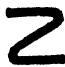
\includegraphics[keepaspectratio]{images/part002_764ec905.jpg}}

把“群”换成“环”、“子群”换成“理想”（左理想或右理想），就得到类似的结果；关于模与代数的类似结果，我们留给读者去陈述。

\subsection{拓扑群与带算子空间的逆极限}

我们将说，逆系统 \((\mathbf{G}_{\alpha}, f_{\alpha\beta})\) 是一个拓扑群的逆系统，如果诸 \(G_{\alpha}\) 是拓扑群且诸 \(f_{\alpha\beta}\) 是连续同态。此时 \(G = \varprojlim G_{\alpha}\) 是积群 \(\prod_{\alpha} G_{\alpha}\) 的一个子群；若给 G 赋以由 \(\prod_{\alpha} G_{\alpha}\) 诱导的拓扑群结构，则如此得到的拓扑群称为拓扑群的逆系统 \((\mathbf{G}_{\alpha}, f_{\alpha\beta})\) 的逆极限。若诸 \(G_{\alpha}\) 是豪斯多夫的（相应地，豪斯多夫且完备的），则 G 是豪斯多夫的且在 \(\prod_{\alpha} G_{\alpha}\) 中闭（相应地，豪斯多夫且完备的）（第一章，§ 8，第 2 节，命题 7 的推论 2 以及第二章，§ 3，第 5 节，命题 10 的推论）。

若 \((\mathbf{G}_{\alpha}^{\prime}, f_{\alpha\beta}^{\prime})\) 是另一个拓扑群的逆系统，且对每个 \(\alpha\) ，\(u_{\alpha}: G_{\alpha} \to G_{\alpha}^{\prime}\) 是一个连续同态，使得诸 \(u_{\alpha}\) 构成映射的逆系统，则 \(u = \varprojlim u_{\alpha}\) 是 G 到 \(G^{\prime} = \varprojlim G_{\alpha}^{\prime}\) 中的一个连续同态（第一章，§ 4，第 4 节）。当把“拓扑群”换成“拓扑环”时，同样的结果成立；关于拓扑模的类似结果，我们留给读者去陈述（§ 6，第 6 节）。

设 \((\mathbf{X}_{\alpha}, g_{\alpha \beta})\) 是拓扑空间的逆系统，\((\mathbf{G}_{\alpha}, f_{\alpha \beta})\) 是拓扑群的逆系统。设每个 \(\mathbf{G}_{\alpha}\) 连续地作用于 \(\mathbf{X}_{\alpha}\) （§ 2，第 4 节），且关系 (1) 对所有 \(x_{\beta} \in \mathbf{X}_{\beta}\) 、\(s_{\beta} \in \mathbf{G}_{\beta}\) 与 \(\alpha \leqslant \beta\) 成立。我们已经看到（第 1 节），\(\mathbf{X} = \varprojlim \mathbf{X}_{\alpha}\) 以 \(\mathbf{G} = \varprojlim \mathbf{G}_{\alpha}\) 为算子群；而且 \(\mathbf{G}\) 连续地作用于 \(\mathbf{X}\) 。因为，若 \(g_{\alpha}\) （相应地，\(f_{\alpha}\) ）是典范映射 \(\mathbf{X} \to \mathbf{X}_{\alpha}\) （相应地，\(\mathbf{G} \to \mathbf{G}_{\alpha}\) ），则按定义

\[
g _ {\alpha} (s, x) = f _ {\alpha} (s). g _ {\alpha} (x)
\]

因而诸映射 \((s.x) \to g_{\alpha}(s.x)\) 在 \(\mathbf{X} \times \mathbf{G}\) 上连续，这表明 \((s, x) \to (s.x)\) 的连续性（第一章，§ 4，第 4 节）。

映射 \(h_{\alpha}: \mathbf{X} / \mathbf{G} \to \mathbf{X}_{\alpha} / \mathbf{G}_{\alpha}\) （它由 \(f_{\alpha}\) 与 \(g_{\alpha}\) 诱导）因此是连续的（§ 2，第 4 节），而映射 \(h: \mathbf{X} / \mathbf{G} \to \varprojlim \mathbf{X}_{\alpha} / \mathbf{G}_{\alpha}\) （它由诸 \(h_{\alpha}\) 定义）也是连续的（第一章，§ 2，第 3 节，命题 4）。

命题 1. 设诸 \(\mathbf{X}_{\alpha}\) 与诸 \(\mathbf{G}_{\alpha}\) 满足上述假设。a) 若 \(\mathbf{X}_{\alpha}\) 的每一点的稳定子群都是 \(\mathbf{G}_{\alpha}\) 的一个紧子群（对每个 \(\alpha \in \mathbf{I}\) ），则每一点 \(x = (x_{\alpha})\) （属于 \(\mathbf{X}\) ）的稳定子群是 \(\mathbf{G}\) 的一个紧子群；\(x\) 的轨道（关于 \(\mathbf{G}\) 的）典范地同胚于诸 \(x_{\alpha}\) 的轨道（关于 \(\mathbf{G}_{\alpha}\) 的）的逆极限；且典范映射 \(h: \mathbf{X} / \mathbf{G} \to \varprojlim \mathbf{X}_{\alpha} / \mathbf{G}_{\alpha}\) 是单射的。

\begin{enumerate}
\def\labelenumi{\alph{enumi})}
\setcounter{enumi}{1}
\tightlist
\item
  若对每个 \(\alpha \in \mathbf{I}\) ，\(\mathbf{X}_{\alpha}\) 的点的每个轨道（关于 \(\mathbf{G}_{\alpha}\) 的）都是紧的，则 \(\mathbf{X}\) 的点的每个轨道（关于 \(\mathbf{G}\) 的）都是相对紧的，且 \(h\) 是满射的。若此外 \(h\) 还是双射的，则 \(\mathbf{X}\) 的点的每个轨道都是紧的。
\end{enumerate}

设 \(x = (x_{\alpha}) \in \mathbf{X}\) ，且对每个 \(\alpha \in \mathbf{I}\) ，设 \(\mathbf{X}_{\alpha}' = \mathbf{G}_{\alpha}.x_{\alpha}\) 为 \(x_{\alpha}\) 的轨道。若 \(\alpha \leqslant \beta\) ，则由 (1) 及关系 \(g_{\alpha\beta}(x_{\beta}) = x_{\alpha}\) 推出 \(g_{\alpha\beta}(\mathbf{X}_{\beta}') \subset \mathbf{X}_{\alpha}',\) 因而 \((\mathbf{X}_{\alpha}')\) 是诸 \(\mathbf{X}_{\alpha}\) 的子集的一个逆系统。对每个 \(\alpha \in \mathbf{I}\) ，设 \(u_{\alpha}: \mathbf{G}_{\alpha} \to \mathbf{X}_{\alpha}'\) 是连续映射 \(s_{\alpha} \to s_{\alpha}.x_{\alpha}\) ；诸 \(u_{\alpha}\) 构成映射的逆系统，而 \(u = \varprojlim u_{\alpha}\) 是连续映射 \(s \to s.x\) ，它把 \(G\) 映入子空间 \(X' = \varprojlim X_{\alpha}'\) （含于 \(X\) ）。a) 的假设蕴含 \(\overline{u}_{\alpha}^{-1}(y_{\alpha})\) 对每个 \(y_{\alpha} \in X_{\alpha}'\) 是紧的。由于 \(u_{\alpha}\) 还是满射的，第一章 § 9 第 6 节命题 8 推论 2 的条件得到满足，因而 a) 的前两个断言成立。于是，若 \(x = (x_{\alpha})\) 与 \(y = (y_{\alpha})\) 使得 \(x_{\alpha}\) 与 \(y_{\alpha}\) 属于关于 \(G_{\alpha}\) 的同一轨道（对每个 \(\alpha \in I\) ），则 \(x\) 与 \(y\) 属于关于 \(G\) 的同一轨道，因此 \(h\) 是单射的。

同样，b) 的假设蕴含：典范映射 \(v_{\alpha}: \mathbf{X}_{\alpha} \to \mathbf{X}_{\alpha}/\mathbf{G}_{\alpha}\) 的逆系统满足第一章 § 9 第 6 节命题 8 推论 2 的条件，因而其逆极限 \(v = \varprojlim v_{\alpha}: \mathbf{X} \to \varprojlim \mathbf{X}_{\alpha}/\mathbf{G}_{\alpha}\) 是满射的，且每一点在 \(v\) 下的逆像都是紧的，这里点取遍 \(\varprojlim X_{\alpha}/G_{\alpha}\) 。由于 \(v\) 分解为

\[
\mathrm{X} \xrightarrow {\psi} \mathrm{X} / \mathrm{G} \xrightarrow {h} \varprojlim \mathrm{X} _ {\alpha} / \mathrm{G} _ {\alpha},
\]

其中 \(\psi\) 是典范映射，b) 的各断言由此得出。

推论 1. 若诸 \(\mathbf{G}_{\alpha}\) 是紧的而诸 \(\mathbf{X}_{\alpha}\) 是豪斯多夫的，则 a) 与 b) 的结论成立。

因为 a) 与 b) 的假设都满足：\(G_{\alpha}\) 的每个闭子群都是紧的，且 \(u_{\alpha}: s_{\alpha} \to s_{\alpha}.x_{\alpha}\) 是紧空间到豪斯多夫空间中的连续映射。

推论 2. 若对每个 \(\alpha \in I\) ，群 \(G_{\alpha}\) 传递地作用于空间 \(X_{\alpha}\) ，且 \(X_{\alpha}\) 的每一点的稳定子群都是 \(G_{\alpha}\) 的紧子群，则 \(G\) 传递地作用于 \(X\)，且 \(X\) 的每一点的稳定子群都是 \(G\) 的紧子群。

因为假设 \(a)\) 满足，且 \(\mathbf{X}_{\alpha}^{\prime} = \mathbf{X}_{\alpha}\) （对每个 \(\alpha\) ）。

推论 3. 设诸 \(\mathbf{G}_{\alpha}\) 是豪斯多夫的。对每个 \(\alpha \in \mathbf{I}\) ，设 \(\mathbf{K}_{\alpha}\) 是 \(\mathbf{G}_{\alpha}\) 的一个紧子群，使得 \(f_{\alpha \beta}(\mathbf{K}_{\beta}) \subset \mathbf{K}_{\alpha}\) 对一切 \(\alpha \leqslant \beta\) 成立。那么，若 \(\mathbf{K} = \varprojlim \mathbf{K}_{\alpha}\) ，则典范映射 \(h\) （它把齐性空间 \(\mathbf{G} / \mathbf{K}\) 映到 \(\varprojlim \mathbf{G}_{\alpha} / \mathbf{K}_{\alpha}\) 中）是一个同胚。

\(h\) 是双射这一事实由推论 1 得出，只需把 \(\mathbf{X}_{\alpha}\) 换成 \(\mathbf{G}_{\alpha}\) ，并把 \(\mathbf{G}_{\alpha}\) 换成以右平移作用的 \(\mathbf{K}_{\alpha}\) （§ 2，第 5 节）。设 \(\varphi\) 是典范映射 \(\mathbf{G} \to \mathbf{G} / \mathbf{K}\) ，且对每个 \(\alpha\) ，设 \(f_{\alpha}\) 是典范映射 \(\mathbf{G} \to \mathbf{G}_{\alpha}\) 。若对每个 \(\alpha, \mathbf{V}_{\alpha}\) 取遍 \(e_{\alpha}\) （\(\mathbf{G}_{\alpha}\) 的单位元）的邻域组成的一个基本系，则诸集合 \(\mathbf{V} = \overline{f}_{\alpha}^{-1}(\mathbf{V}_{\alpha}) (\alpha \text{与} \mathbf{V}_{\alpha} \text{变动})\) 构成 \(e\) （\(\mathbf{G}\) 的单位元）的邻域基本系（第一章，§ 4，第 4 节，命题 9），而诸集合 \(\varphi(\mathbf{V}.K)\) 构成 \(\varphi(e)\) 在 \(G/K\) 中的邻域基本系。我们要证明 \(\varphi(V.K)\) 在 \(h\) 下的像包含 \(h(\varphi(e))\) 的一个邻域，亦即存在 \(\beta \geqslant \alpha\) 和一个邻域 \(W_{\beta}\) （\(e_{\beta}\) 在 \(G_{\beta}\) 中），使得 \(\overline{f}_{\beta}^{-1}(W_{\beta}.K_{\beta}) \subset V.K\) 。现在，关系 \(x \in V.K\) 等价于存在 \(y\) （属于 \(K\) ），使 \(f_{\alpha}(xy^{-1}) \in V_{\alpha}\) ，即 \(f_{\alpha}(x) \in V_{\alpha}.f_{\alpha}(K)\) ；从而 \(V.K = \overline{f}_{\alpha}^{-1}(V_{\alpha}.f_{\alpha}(K))\) 。令 \(U_{\alpha} = V_{\alpha}.f_{\alpha}(K)\) ；我们将看到，存在 \(\beta \geqslant \alpha\) ，使得当令 \(U_{\beta} = \overline{f}_{\alpha\beta}^{-1}(U_{\alpha})\) 时有 \(K_{\beta} \subset U_{\beta}\) ；于是将可推出存在一个邻域 \(W_{\beta}\) （\(e_{\beta}\) 在 \(G_{\beta}\) 中），使 \(W_{\beta}.K_{\beta} \subset U_{\beta}\) （第二章，§ 4，第 3 节，命题 4 的推论），而这便建立了所要的关系

\[
\overline {{f}} _ {\beta} ^ {-1} (\mathrm{W} _ {\beta}. \mathrm{K} _ {\beta}) \subset \overline {{f}} _ {\beta} ^ {-1} (\mathrm{U} _ {\beta}) = \mathrm{V}. \mathrm{K}.
\]

我们用反证法来进行：对每个 \(\beta \geqslant \alpha\) ，用 \(\mathbf{M}_{\beta}\) 表示 \(\mathbf{K}_{\beta} \cap \mathbb{C}\mathbf{U}_{\beta}\) ；由于 \(\overline{f}_{\beta \gamma}^{-1}(\mathrm{U}_{\beta}) = \mathrm{U}_{\gamma}\) （当 \(\alpha \leqslant \beta \leqslant \gamma\) 时），诸 \(\mathbf{M}_{\beta}\) 构成诸 \(\mathbf{G}_{\beta}\) 的紧子集的一个逆系统（对 \(\beta \geqslant \alpha\) ）。如果它们都非空，则它们的逆极限 \(\mathbf{M}\) 也非空（第一章，§ 9，第 6 节，命题 8）。显然 \(\mathbf{M} \subset \mathbf{K}\) 且 \(f_{\alpha}(\mathbf{M}) \subset \mathbf{M}_{\alpha}\) ；但这是荒谬的，因为 \(f_{\alpha}(\mathbf{K}) \subset \mathbf{U}_{\alpha}\) ，于是证明完毕。

\subsection{拓扑群的逼近}

设 G 是一个群，并设 \((\mathrm{H}_{\alpha})_{\alpha\in\mathbf{I}}\) 是 G 的正规子群的一个族，使得 \(H_{\alpha}\supset H_{\beta}\) 对一切 \(\alpha\leqslant\beta\) 成立。对每个 \(\alpha\in I\) ，令 \(G_{\alpha}=G/H_{\alpha}\) ；而对 \(\alpha\leqslant\beta\) ，令 \(f_{\alpha\beta}\) 为典范同态 \(G/H_{\beta}\to G/H_{\alpha}\) ，它因而把 \(H_{\beta}\) 在 G 中的一个陪集 T 映为陪集 \(TH_{\alpha}\) （\(H_{\alpha}\) 在 G 中的）。显然 \((G_{\alpha},f_{\alpha\beta})\) 是群的一个逆系统；\(\tilde{G}=\varprojlim G_{\alpha}\) 的元素是诸族 \((T_{\alpha})_{\alpha\in\mathbf{I}}\) ，其中 \(T_{\alpha}\) 是 \(H_{\alpha}\) 在 G 中的一个陪集（对每个 \(\alpha\) ），且 \(T_{\alpha}\supset T_{\beta}\) 对一切 \(\alpha\leqslant\beta\) 成立。映射 \(i:s\to(sH_{\alpha})\) （它把 G 映入 \(\tilde{G}\) ）是诸典范同态 \(G\to G/H_{\alpha}\) 的逆极限，因而是 G 到 \(\tilde{G}\) 中的一个同态，且元素 \((T_{\alpha})\in\tilde{G}\) 在 i 下的逆像等于 \(\bigcap_{\alpha\in I}T_{\alpha}\) 。于是 i 的核是 \(\bigcap_{\alpha\in I}H_{\alpha}\) ，而 i 的像由交非空的诸族 \((T_{\alpha})\in\tilde{G}\) 组成。

现在设 G 是一个拓扑群；若给每个 \(G_{\alpha} = G/H_{\alpha}\) 赋以商拓扑，则显然 \((\mathbf{G}_{\alpha}, f_{\alpha\beta})\) 是拓扑群的一个逆系统，且 \(i : G \to \tilde{G}\) 是一个连续同态。

命题 2. 设 G 是一个拓扑群，并设 \((\mathrm{H}_{\alpha})_{\alpha\in I}\) 是 G 的正规子群的一个族，使得 \(H_{\alpha}\supset H_{\beta}\) 对一切 \(\alpha\leqslant\beta\) 成立，且满足下面的条件：

(AP) 对每个 \(\alpha \in I\) ，\(H_{\alpha}\) 在 G 中闭，且 G 中单位元 \(e\) 的每个邻域都包含诸 \(H_{\alpha}\) 之一（换言之，诸 \(H_{\alpha}\) 组成的滤基收敛于 \(e\) ）。

那么，映射 \(i: \mathbf{G} \to \tilde{\mathbf{G}} = \varprojlim \mathbf{G} / \mathbf{H}_{\alpha}\) 是 \(\mathbf{G}\) 到 \(i(\mathbf{G})\) 上的一个严格态射；\(\tilde{\mathbf{G}}\) 是豪斯多夫的，且 \(i(\mathbf{G})\) 在 \(\tilde{\mathbf{G}}\) 中稠密；最后，\(i\) 的核是 \(\{e\}\) 在 \(\mathbf{G}\) 中的闭包。此外，若诸 \(\mathbf{H}_{\alpha}\) 中有一个是完备的，则 \(i\) 是满射的。

显然诸 \(G_{\alpha} = G/H_{\alpha}\) 是豪斯多夫的（§ 2，第 5 节，命题 13），因而 \(\tilde{G}\) 也是（因为它是 \(\prod_{\alpha \in I} G_{\alpha}\) 的一个子空间）。i 的核 H 是诸 \(H_{\alpha}\) 的交，因而是 G 的一个闭子群。由于 \(e\) 的每个邻域都包含某个 \(H_{\alpha}\) ，它包含 \(H\) ，因此{[}§ 3，第 1 节，公式 (1){]}\(H\) 是 \(\{e\}\) 的闭包。接下来我们证明 \(i(G)\) 在 \(\tilde{G}\) 中稠密。设 \(f_{\alpha}\) 是典范映射 \(\tilde{G} \to G_{\alpha}\) ，它是 \(\tilde{G}\) 上射影 \(pr_{\alpha}\) 的限制；\(\varphi_{\alpha} = f_{\alpha} \circ i\) 是典范映射 \(G \to G / H_{\alpha}\) 。若 \(U\) 是 \(\tilde{G}\) 的任一非空开集，则存在指标 \(\alpha \in I\) 与非空开集 \(U_{\alpha}\) （在 \(G_{\alpha}\) 中），使得 \(\overline{f}_{\alpha}^{-1}(U_{\alpha}) \subset U\) （第一章，§ 4，第 4 节，命题 9）；因而

\[
\overline {{i}} ^ {-1} (\mathbf {U}) \supset \overline {{\varphi}} _ {\alpha} ^ {-1} (\mathbf {U} _ {\alpha});
\]

但由于 \(\varphi_{\alpha}\) 是满射的，\(\overline{i}^{-1}(\mathbf{U})\) 非空，因而 \(i(\mathbf{G}) \cap \mathbf{U} \neq \emptyset\) 。为看出 \(i\) 是 \(\mathbf{G}\) 到 \(i(\mathbf{G})\) 上的一个严格态射，考虑一个邻域 \(\mathbf{V}\) （\(e\) 在 \(\mathbf{G}\) 中的）。存在一个邻域 \(\mathbf{W}\) （\(e\) 在 \(\mathbf{G}\) 中的），使得 \(\mathbf{W}^2 \subset \mathbf{V}\) ，又存在指标 \(\alpha \in \mathbf{I}\) ，使得 \(\mathbf{H}_{\alpha} \subset \mathbf{W}\) ；由此推出 \(\mathbf{V}\) 包含 \(\mathrm{WH}_{\alpha} = \overline{\varphi}_{\alpha}^{-1}(\varphi_{\alpha}(\mathbf{W})) = \overline{i}^{-1}(\overline{f}_{\alpha}^{-1}(\varphi_{\alpha}(\mathbf{W})))\) 。由于 \(\overline{f}_{\alpha}^{-1}(\varphi_{\alpha}(\mathbf{W}))\) 是 \(\tilde{\mathbf{G}}\) 中单位元的一个邻域，结论得证。

最后，假设存在指标 \(\gamma \in I\) ，使得 \(H_{\gamma}\) 是完备的。为证明 \(i\) 是满射的，只需证明每个族 \((T_{\alpha})_{\alpha \in I} \in \tilde{G}\) 有非空的交。由于 \(T_{\gamma}\) 是由 \(H_{\gamma}\) 经平移得到的，它是 \(G\) 的一个完备子空间（关于右一致结构与左一致结构两者）。此外，由于每个邻域 \(U\) （\(e\) 在 \(G\) 中的）都包含诸 \(H_{\alpha}\) 之一，相应的集合 \(T_{\alpha}\) 是 \(U_{d-}\) （或 \(U_{s-}\) ）小的，因而诸 \(T_{\alpha}\) （含于 \(T_{\gamma}\) 者）所成之集是一个柯西滤基；故它在 \(T_{\gamma}\) 中收敛，又由于诸 \(T_{\alpha}\) 在 \(G\) 中闭（因为它们是诸 \(H_{\alpha}\) 的平移），它们的交非空。

证毕。

推论 1. 若条件 (AP) 满足，且此外诸（豪斯多夫）群 \(\mathbf{G} / \mathbf{H}_{\alpha}\) 都是完备的，则群 \(\mathbf{G}\) 有一个可等同于 \(\tilde{\mathbf{G}}\) 的豪斯多夫完备化；且映射 \(i: \mathbf{G} \to \tilde{\mathbf{G}}\) 那时可等同于典范映射（§ 3，第 3 节，命题 5）。

因为此时 \(\tilde{\mathbf{G}}\) 是完备的（第 2 节），且命题 2 表明 \(i(\mathbf{G})\) 同构于由 \(\mathbf{G}\) 得到的豪斯多夫群；由于它在 \(\tilde{\mathbf{G}}\) 中稠密，推论得证（\(\S 3\) ，第 3 节，命题 5）。特别地：

推论 2. 设 G 是一个群，并设 \((\mathrm{H}_{\alpha})\) 是 G 的正规子群的一个族，它关于关系 \(\mathrm{H}_{\alpha} \supset \mathrm{H}_{\beta}\) 有向。若给 G 赋以使诸 \(\mathrm{H}_{\alpha}\) 构成单位元 \(e\) 的邻域基本系的群拓扑，则 G 的相伴豪斯多夫群同构于 \(\mathrm{G}_{1} = \mathrm{G} / \left( \bigcap_{\alpha} \mathrm{H}_{\alpha} \right)\) ；\(\mathrm{G}_{1}\) 有一个完备化 \(\hat{\mathrm{G}}_{1} = \tilde{\mathrm{G}}\) ；且典范映射 \(\mathrm{G}_{1} \to \hat{\mathrm{G}} = \varprojlim \mathrm{G} / \mathrm{H}_{\alpha}\) 可延拓为 \(\hat{\mathrm{G}} = \hat{\mathrm{G}}_{1}\) 到 \(\tilde{\mathrm{G}}\) 上的一个同构。

G 的子群 \(H_{\alpha}\) 是开的，因而也是闭的（\(\S\) 2，第 1 节，命题 4 的推论），且 \(G/H_{\alpha}\) 是离散的（\(\S\) 2，第 6 节，命题 18）；于是推论 1 的条件得到满足。

在本小节的其余部分，我们将假设 G 是豪斯多夫的，且 \((\mathbf{H}_{\alpha})\) 是 G 的紧正规子群的一个族，它关于关系 \(H_{\alpha} \supset H_{\beta}\) 有向并满足条件 (AP)；根据命题 2，映射

\[
i: \mathrm{G} \rightarrow \tilde {\mathrm{G}} = \varprojlim \mathrm{G} / \mathrm{H} _ {\alpha}
\]

于是是一个拓扑群的同构，它使我们可以把 G 与 \(\tilde{G}\) 等同起来。我们用 \(f_{\alpha}\) 表示典范映射 \(G \rightarrow G/H_{\alpha}\) 。

引理 1. 在命题 2 的假设下，若 E 是 G 的任一闭子集，我们有 \(\mathbf{E} = \bigcap_{\alpha} \mathrm{EH}_{\alpha}\) 。

因为 E 是诸集合 EV 的交，这里 V 取遍 e 的邻域滤子{[}§ 3，第 1 节，公式 (1){]}，且 e 的每个邻域都包含某个 \(H_{\alpha}\) ；又因 \(E \subset EH_{\alpha}\) ，结论得证。

命题 3. 假设 G 是豪斯多夫的，且诸 \(H_{\alpha}\) 是紧的并满足 (AP)。

\begin{enumerate}
\def\labelenumi{\alph{enumi})}
\item
  设 L 是 G 的一个闭子群；则对每个 \(\alpha\in I\) ，子群 \(L_{\alpha}=f_{\alpha}(L)\) （\(G_{\alpha}=G/H_{\alpha}\) 中的）是闭的，且 G 到 \(\varprojlim G_{\alpha}\) 上的同构 i 经限制给出 L 到 \(\varprojlim L_{\alpha}\) 上的一个同构。若还有 L 在 G 中正规，则 \(L_{\alpha}\) 在 \(G_{\alpha}\) 中正规（对每个 \(\alpha\in I\) ），且过渡到商，i 诱导出 G/L 到 \(\varprojlim G_{\alpha}/L_{\alpha}\) 上的一个同构。
\item
  反之，对每个 \(\alpha \in I\) ，设 \(L_{\alpha}\) 是 \(G_{\alpha}\) 的一个闭子群，使得 \(L_{\alpha} = f_{\alpha \beta}(L_{\beta})\) 对一切 \(\alpha \leqslant \beta\) 成立。则存在唯一的闭子群 \(L\) （\(G\) 中的），使得 \(L_{\alpha} = f_{\alpha}(L)\) 对每个 \(\alpha \in I\) 成立；而若此外 \(L_{\alpha}\) 在 \(G_{\alpha}\) 中正规（对每个 \(\alpha \in I\) ），则 \(L\) 在 \(G\) 中正规。
\item
  由于 \(\mathbf{H}_{\alpha}\) 是紧的，\(\mathrm{LH}_{\alpha}\) 在 \(\mathbf{G}\) 中闭（\(\S 4\) ，第 1 节，命题 1 的推论 1），因而 \(\mathbf{L}_{\alpha}\) 在 \(\mathbf{G}_{\alpha}\) 中闭。由于 \(i\) 把拓扑群 \(\mathbf{G}\) 与 \(\varprojlim \mathbf{G}_{\alpha}\) 等同起来，且 \(\varprojlim \mathbf{L}_{\alpha}\) 可与 \(\varprojlim \mathbf{G}_{\alpha}\) 的一个（拓扑）子群等同，\(i\) 把子群 \(\bigcap_{\alpha} \mathrm{LH}_{\alpha}\) （\(\mathbf{G}\) 的）与 \(\varprojlim \mathbf{L}_{\alpha}\) 等同起来，而为证明第一个断言，只需注意由引理 1 有 \(\mathbf{L} = \bigcap_{\alpha} \mathrm{LH}_{\alpha}\) 。另一方面，若 \(\mathbf{L}\) 正规，则对每个 \(\alpha \in \mathbf{I}\) ，映射 \(f_{\alpha}': \mathbf{G} / \mathbf{L} \to \mathbf{G}_{\alpha} / \mathbf{L}_{\alpha}\) （它由 \(f_{\alpha}\) 诱导）是一个满射的严格态射（\(\S 2\) ，第 8 节，注 3），其核是紧正规子群 \(\mathrm{H}_{\alpha} \mathrm{L} / \mathrm{L}\) （\(\mathrm{G} / \mathrm{L}\) 的），即紧子群 \(\mathrm{H}_{\alpha}\) （\(\mathbf{G}\) 的）的典范像。由于诸子群 \(\mathrm{H}_{\alpha} \mathrm{L} / \mathrm{L}\) （\(\mathrm{G} / \mathrm{L}\) 的）满足条件 (AP)（§ 2，第 8 节，命题 24），且 G/L 是豪斯多夫的，a) 的最后一个断言是命题 2 的推论。
\item
  设 \(f_{\alpha \beta}'\) 是 \(f_{\alpha \beta}\) 到 \(\mathbf{L}_{\beta} (\alpha \leqslant \beta)\) 上的限制。则 \((\mathbf{L}_{\alpha}, f_{\alpha \beta}')\) 是拓扑群的一个逆系统，其逆极限 \(\mathbf{L}\) 可与子群 \(\mathbf{G} \cap \prod_{\alpha} \mathbf{L}_{\alpha}\) （\(\mathbf{G}\) 的）等同。据假设，\(f_{\alpha \beta}'\) 是满射的，且其核是紧子群 \(f_{\beta}(\mathrm{H}_{\alpha}) \cap \mathrm{L}_{\beta}\) （\(\mathbf{L}_{\beta}\) 的）；因而（第一章，§ 9，第 6 节，命题 8 的推论 1）我们有 \(\mathbf{L}_{\alpha} = f_{\alpha}(\mathbf{L})\) ，对一切 \(\alpha \in \mathbf{I}\) 成立。若 \(\mathbf{L}'\) 是 \(\mathbf{G}\) 的另一个闭子群，使得 \(f_{\alpha}(\mathbf{L}') = \mathbf{L}_{\alpha}\) 对一切 \(\alpha \in \mathbf{I}\) 成立，则 \(\mathbf{L}'\mathbf{H}_{\alpha} = \overline{f}_{\alpha}^{-1}(\mathbf{L}_{\alpha})\) ，从而（引理 1）\(\mathbf{L}' = \bigcap_{\alpha} \mathbf{L}'\mathbf{H}_{\alpha} = \bigcap_{\alpha} \overline{f}_{\alpha}^{-1}(\mathbf{L}_{\alpha}) = \mathbf{L}\) 。最后，b) 的最后一个断言由公式 \(\mathbf{L} = \bigcap_{\alpha} \overline{f}_{\alpha}^{-1}(\mathbf{L}_{\alpha})\) 得出，因为诸 \(\overline{f}_{\alpha}^{-1}(\mathbf{L}_{\alpha})\) 现在是 \(\mathbf{G}\) 的正规子群。
\end{enumerate}

命题 4. 假设 G 是豪斯多夫的，诸 \(H_{\alpha}\) 是紧的，且 (AP) 满足。若 \(C_{\alpha}\) 是 \(G_{\alpha} = G/H_{\alpha}\) 的单位分量，则 G 的单位分量 C 可与 \(\varprojlim C_{\alpha}\) 等同，且我们有 \(f_{\alpha}(C) = C_{\alpha}\) 。本命题是下述引理的推论：

引理 2. 设 G 是一个豪斯多夫拓扑群，H 是 G 的一个紧正规子群，\(\varphi\) 是典范映射 \(\mathbf{G} \to \mathbf{G} / \mathbf{H}\) 。若 C 是 G 的单位分量，则 \(\varphi(\mathbf{C})\) 是 \(\mathbf{G}' = \mathbf{G} / \mathbf{H}\) 的单位分量。

一旦建立了这个引理，我们就将有 \(f_{\alpha}(\mathbf{C}) = \mathbf{C}_{\alpha}\) （对每个 \(\alpha \in \mathbf{I}\) ），且由于 \(\mathbf{C}\) 是 \(\mathbf{G}\) 的一个闭子群（§ 2，第 2 节，命题 7），只需应用命题 3a)。

为证明引理，首先注意，若 \(C'\) 是 \(e'\) 在 \(G'\) 中的连通分量，则 \(\varphi(C) \subset C'\) ，因为 \(\varphi(C)\) 是连通的。假设 \(\varphi(C) \neq C'\) 。由于 C 是 G 的一个闭正规子群（§2，第 2 节，命题 7），\(\varphi(C)\) 是 \(G'\) 的一个正规子群；若 \(\psi\) 是典范映射 \(G' \to G'/\varphi(C)\) ，则 \(\psi(C')\) 是连通的且不只由单位元组成；因而 \(G'/\varphi(C)\) 的单位分量不只由单位元组成。但 \(G'/\varphi(C)\) 同构于 \((G/H)/(HC/H)\) ，从而同构于 G/HC，于是也同构于 \((G/C)/(HC/C)\) （§2，第 7 节，命题 22 的推论以及命题 20）。现在，G/C 是豪斯多夫的且全不连通的（第一章，§11，第 5 节，命题 9），而 HC/C 作为 G 的紧正规子群 H 的典范像，是 G/C 的一个紧子群。因此只需在附加假设 G 全不连通、即 \(C = \{e\}\) 之下证明引理 2。

于是设 \(C' \neq \{e'\}\) ；把 G 换成它的子群 \(\varphi^{-1}(C')\) （它全不连通且包含 H），我们就可以假设 \(G'\) 是连通的且不止由一点组成。

设 \(\mathfrak{M}\) 是由闭子群 \(L\) （\(G\) 中的）组成的集合，这些子群满足 \(LH = G\) 。我们将证明 \(\mathfrak{M}\) 按关系 \(\supset\) 排序是归纳的。事实上，若 \(\mathfrak{X}\) 是 \(\mathfrak{M}\) 的一个线性有序子集，则对每个 \(x \in G\) ，诸集合 \(xH \cap L\) （\(L \in \mathfrak{X}\)）组成的集是一个由紧空间 \(xH\) 中的闭集组成的滤基；因而这些集合的交非空，这表明诸子群 \(L \in \mathfrak{X}\) 的交属于 \(\mathfrak{M}\) 。应用佐恩引理，我们因此看出 \(\mathfrak{M}\) 有一个极小元 \(L_0\) 。由于 \(H\) 是紧的，\(G/H = L_0H/H\) 同构于 \(L_0/(L_0 \cap H)\) （\(\S 4\) ，第 1 节，命题 1 的推论 3）；由于 \(L_0\) 全不连通且 \(L_0 \cap H\) 是紧的，我们看出可以把 \(G\) 换成 \(L_0\) ；换言之，我们可以附加假设不存在闭子群 \(L \neq G\) 满足 \(LH = G\) 。

现在设 F 是 G 中既开又闭的单位元的诸邻域的交，我们来证明 F 是 G 的一个闭子群。显然 F 在 G 中闭；因而只需证明 \(F^{-1}.F \subset F\) 。但若 \(x \in F\) 且 V 是 e 在 G 中的一个既开又闭的邻域，则 xV 也是；否则 e 将属于 xV 在 G 中的余集 W，而 W 又是既开又闭的，且我们将有 \(x \notin W\) ；从而 \(x \notin F\) ，与假设矛盾。由此推出 xF（诸集合 xV 的交，V 取遍 e 在 G 中的既开又闭的邻域）包含 F；换言之，\(x^{-1}F \subset F\) ，这就证明了我们的断言。由于 G 全不连通且 \(G \neq \{e\}\) ，我们有 \(F \neq G\) 。但若 V 是 e 在 G 中的一个既开又闭的邻域，则 VH 在 G 中也是既开又闭的（§ 4，第 1 节，命题 1 的推论 1），因而 \(\varphi(V)\) 在 G/H 中既开又闭，而这在假设之下蕴含 \(\varphi(V) = G/H\) 。我们将由此推出 FH = G，它将给出所要的矛盾并完成引理的证明。事实上，对每个 \(x \in G\) ，xH 与 e 的每个既开又闭的邻域 V 相交，因而也与这些邻域的交 F 相交，因为诸集合 \(Vx \cap H\) 组成一个由紧空间 xH 中的闭集组成的滤基。

证毕。

注. 若子群 \(H_{\alpha}\) 对某个 \(\alpha \in I\) 是紧的，则 \(H_{\beta}\) 对一切 \(\beta \geqslant \alpha\) 是紧的，因为它是 \(H_{\alpha}\) 的一个闭子群。由于所有 \(\beta \in I\) （满足 \(\beta \geqslant \alpha\) 的）组成的集合在 I 中共尾，在群 G 的研究中，假设诸 \(H_{\alpha}\) 之一是紧的与假设所有 \(H_{\alpha}\) 都是紧的，本质上有同样的结果。

\subsection{在逆极限上的应用}

命题 5. 设 \((\mathbf{G}_{\alpha}, f_{\alpha \beta})\) 是豪斯多夫拓扑群的一个逆系统，使得诸 \(f_{\alpha \beta}\) 是核紧的满射严格态射。则对每个 \(\alpha \in I\) ，典范映射 \(f_{\alpha}\) （它把 \(\mathbf{G} = \varprojlim \mathbf{G}_{\alpha}\) 映入 \(\mathbf{G}_{\alpha}\) ）是一个核紧的满射严格态射。

\(f_{\alpha}\) 是满射的且其核是紧的这两件事是第一章 § 9 第 6 节命题 8 推论 1 的推论。剩下的只是证明 \(f_{\alpha}\) 是一个严格态射。用 \(e\) （相应地，\(e_{\alpha}\) ）表示 G （相应地，\(G_{\alpha}\) ）的单位元。G 中 \(e\) 的每个邻域 V 包含形如 \(\overline{f}_{\beta}^{-1}(V_{\beta})\) 的集合，这里 \(V_{\beta}\) 是 \(e_{\beta}\) 在 \(G_{\beta}\) 中的一个邻域，且我们可以假设 \(\beta \geqslant \alpha\) ；由于 \(f_{\alpha \beta}\) 是满射的严格态射，\(f_{\alpha \beta}(V_{\beta})\) 是 \(e_{\alpha}\) 在 \(G_{\alpha}\) 中的一个邻域，又由于 \(f_{\beta}\) 是满射的，我们有 \(V_{\beta} \subset f_{\beta}(V)\) ，由此

\[
f _ {\alpha} (\mathbf {V}) = f _ {\alpha \beta} (f _ {\beta} (\mathbf {V})) \supset f _ {\alpha \beta} (\mathbf {V} _ {\beta});
\]

这表明 \(f_{\alpha}(\mathbf{V})\) 是 \(e_{\alpha}\) 在 \(\mathbf{G}_{\alpha}\) 中的一个邻域。

若 \(\mathrm{H}_{\alpha}=\overline{f}_{\alpha}^{-1}(e_{\alpha})\) ，则每个 \(H_{\alpha}\) 是 G 的一个紧正规子群；诸 \(H_{\alpha}\) 显然满足第 3 节的条件 (AP)；且 \(G_{\alpha}\) 可与 \(G/H_{\alpha}\) 等同。特别地，第 3 节的命题 3 与命题 4 可应用于 G 与诸 \(H_{\alpha}\) 。

推论 1. 设 \((\mathbf{G}_{\alpha}, f_{\alpha \beta})\) 是满足命题 5 的假设的拓扑群逆系统；设 \((\mathbf{G}_{\alpha}', f_{\alpha \beta}')\) 是拓扑群的一个逆系统，且对每个 \(\alpha\) ，设 \(u_{\alpha}: \mathbf{G}_{\alpha} \to \mathbf{G}_{\alpha}'\) 是核紧的满射严格态射，使得诸 \(u_{\alpha}\) 构成映射的一个逆系统。则 \(u = \varprojlim u_{\alpha}\) 是 \(\mathbf{G} = \varprojlim \mathbf{G}_{\alpha}\) 到 \(\mathbf{G}' = \varprojlim \mathbf{G}_{\alpha}'\) 上的一个严格态射，且其核是紧的。

设 \(N_{\alpha}\) 是 \(u_{\alpha}\) 的核。\(L_{\alpha} = \overline{f}_{\alpha}^{-1}(N_{\alpha})\) 因而是满射严格态射 \(v_{\alpha} = u_{\alpha} \circ f_{\alpha}: G \to G'_{\alpha}\) 的核；由于 \(L_{\alpha}/H_{\alpha}\) 同构于 \(N_{\alpha}\) （§ 2，第 7 节，命题 20），\(L_{\alpha}\) 是 G 的一个紧正规子群（§ 4，第 1 节，命题 2 的推论 2）。u 的核 L 是诸 \(L_{\alpha}\) 的交。用 \(\varphi\) 表示典范映射 \(G \to G/L\) ；则我们可以写 \(v_{\alpha} = w_{\alpha} \circ \varphi\) ，其中 \(w_{\alpha}\) 是 G/L 到 \(G'_{\alpha}\) 上的一个严格态射，其核是 \(L_{\alpha}/L\) 。由于诸 \(L_{\alpha}/L\) 的交是 G/L 的单位元，且诸 \(L_{\alpha}/L\) 组成一个滤基并且是紧的，这个滤基收敛于 G/L 的单位元（第一章，§ 9，第 1 节，定理 1 的推论）。于是第 3 节的命题 2 表明 \(w = \varprojlim w_{\alpha}\) 是 G/L 到 \(G'\) 上的一个同构；由此推出 \(w \circ \varphi\) 是 G 到 \(G'\) 上的一个严格态射，其核为 L。但显然 \(u = w \circ \varphi\) ，这样推论就证明了。

推论 2. 设 \((\mathbf{G}_{\alpha}, f_{\alpha \beta})\) 是满足命题 5 的条件的拓扑群逆系统，并设 \(\mathbf{G}'\) 是一个拓扑群，其中存在一个邻域 \(\mathbf{V}'\) （单位元 \(e'\) 的），它不含 \(\mathbf{G}'\) 的除 \(\{e'\}\) 外的任何子群。那么，若 \(v: \mathbf{G} \to \mathbf{G}'\) 是任一连续同态，则存在指标 \(\alpha \in \mathbf{I}\) 与连续同态 \(v_{\alpha}: \mathbf{G}_{\alpha} \to \mathbf{G}'\) ，使得 \(v = v_{\alpha} \circ f_{\alpha}\) 。

因为由于 \(\overline{v}^{-1}(\mathbf{V}^{\prime})\) 是 \(e\) 在 \(\mathbf{G}\) 中的一个邻域，存在指标 \(\alpha\) 与一个邻域 \(\mathbf{V}_{\alpha}\) （\(e_{\alpha}\) 在 \(\mathbf{G}_{\alpha}\) 中的），使得 \(\overline{f}_{\alpha}^{-1}(\mathbf{V}_{\alpha}) \subset \overline{v}^{-1}(\mathbf{V}^{\prime})\) 。因而 \(v(\mathbf{H}_{\alpha}) \subset \mathbf{V}^{\prime}\) ，且由于 \(v(\mathbf{H}_{\alpha})\) 是 \(\mathbf{G}^{\prime}\) 的一个子群，由此推出 \(v(\mathbf{H}_{\alpha}) = \{e^{\prime}\}\) 。由于 \(f_{\alpha}\) 可与典范映射 \(\mathbf{G} \to \mathbf{G}/\mathbf{H}_{\alpha}\) 等同，本推论是连续同态的典范分解（§ 2，第 8 节）的推论。

\BourbakiExercises
\BourbakiExerciseGroup

\begin{enumerate}
\def\labelenumi{\arabic{enumi})}
\item
  有限群 G 的与群结构相容的每个拓扑，可以这样得到：取包含 G 的一个正规子群 H 的那些集合作为单位元的邻域。
\item
半拓扑群是指一个群 \(\mathbf{G}\) ，带有一个拓扑，使得对每个 \(a \in \mathbf{G}\) ，平移 \(x \to ax\) 与 \(x \to xa\) 都在 \(\mathbf{G}\) 上连续，且对称 \(x \to x^{-1}\) 在 \(\mathbf{G}(*)\) 上连续。
\end{enumerate}

\begin{enumerate}
\def\labelenumi{\alph{enumi})}
\tightlist
\item
  一个滤子 \(\mathfrak{B}\) （在群 \(\mathbf{G}\) 上）是 \(e\) 的邻域滤子（在使 \(\mathbf{G}\) 成为半拓扑群的一个拓扑中），当且仅当 \(\mathfrak{B}\) 满足公理 \((\mathrm{GV}_{\mathrm{I}})\) 与 \((\mathrm{GV}_{\mathrm{III}})\) ，且滤子族
\end{enumerate}

\[
\mathfrak {B} (x) = x. \mathfrak {B} = \mathfrak {B}. x \quad (x \in G)
\]

满足第一章 § 1 第 2 节的公理 \((\mathbf{V}_{\mathbf{IV}})\) 。

\begin{enumerate}
\def\labelenumi{\alph{enumi})}
\setcounter{enumi}{1}
\tightlist
\item
  若 G 是无限群，试证：以 \(\varnothing\) 与 G 的有限子集的余集为开集的那个拓扑，使 G 成为一个非豪斯多夫的半拓扑群，其中 \(\{e\}\) 是闭的，但与 G 的群结构不相容。
\end{enumerate}

\(^{*}c)\) 在 R 上定义一个比通常拓扑更细的拓扑，使 R 成为一个半拓扑群但不是拓扑群{[}考虑一个递减数列 \((r_{n})\) （诸数 \textgreater0 ，趋于 0），并取诸对称区间 {]}-a, a{[} 与点集 \(\pm r_{n}\) 的余集的交）。 *

(*) 若 G 是局部紧的，这些条件蕴含 G 的拓扑与其群结构相容（第十章，§ 3，习题 25）。

\begin{enumerate}
\def\labelenumi{\arabic{enumi})}
\setcounter{enumi}{2}
\item
  设 A 是半拓扑（相应地，拓扑）群 G 的一个子集。若 V 取遍 G 中 e 的邻域滤子，则诸集合 AV 的交、或诸集合 VA （或诸集合 VAV）的交是 A 的闭包 \(\overline{A}\) 。
\item
  仿拓扑群是指一个群 G ，带有一个满足公理 \((\mathrm{GT}_{\mathbf{I}})(*)\) 的拓扑。
\end{enumerate}

\begin{enumerate}
\def\labelenumi{\alph{enumi})}
\item
  一个滤子 \(\mathfrak{B}\) （群 \(G\) 上的）是 \(e\) 的邻域滤子（对应于使 \(G\) 成为仿拓扑群的一个拓扑），当且仅当 \(\mathfrak{B}\) 满足公理 \((\mathrm{GV}_{\mathbf{I}})\) 与 \((\mathrm{GV}_{\mathbf{III}})\) ，且 \(e \in V\) 对一切 \(V \in \mathfrak{B}\) 成立。相应的拓扑则是唯一的；它是豪斯多夫的，当且仅当诸集合 \(V.V^{-1}\) （\(V\) 取遍 \(\mathfrak{B}\) ）的交仅由点 \(e\) 组成。
\item
  在整数群 \(\mathbf{Z}\) 上，设 \(\mathbf{V}_n\) 是由 \(0\) 与所有整数 \(m \geqslant n\) 组成的集合（对每个 \(n > 0\) ）。试证诸 \(\mathbf{V}_n\) 构成 \(0\) 的邻域基本系（对应 \(\mathbf{Z}\) 上一个非豪斯多夫拓扑），且带此拓扑的 \(\mathbf{Z}\) 是一个仿拓扑群，其中 \(\{0\}\) 是闭的。
\item
  仿拓扑群 G 是拓扑群，当且仅当对 G 的每个子集 A ，诸集合 AV （或诸集合 VA）的交是 A 的闭包 \(\overline{A}\) （当 V 取遍 e 的邻域滤子时）。（为看出条件是充分的，取 A 为 e 的一个开邻域的余集。）
\end{enumerate}

\begin{enumerate}
\def\labelenumi{\arabic{enumi})}
\setcounter{enumi}{4}
\tightlist
\item
  设 \(\mathfrak{B}\) 是群 \(\mathbf{G}\) 上的一个滤子，满足公理 \((\mathrm{GV}_{\mathbf{I}})\) 与 \((\mathrm{GV}_{\mathbf{II}})\) 。
\end{enumerate}

\begin{enumerate}
\def\labelenumi{\alph{enumi})}
\tightlist
\item
  存在唯一的拓扑 \(\mathfrak{C}_s\) （相应地，\(\mathfrak{C}_d\) ），它定义在 \(\mathbf{G}\) 上，使得对每个 \(a \in \mathbf{G}\) ，\(a\) 关于 \(\mathfrak{C}_s\) （相应地，\(\mathfrak{C}_d\) ）的邻域滤子是 \(a\) . \(\mathfrak{B}\) （相应地，\(\mathfrak{B}\) . \(a\) ）。
\end{enumerate}

设 \(\mathbf{G}_s\) （相应地，\(\mathbf{G}_d\) ）是通过给 \(\mathbf{G}\) 赋以拓扑 \(\mathcal{C}_s\) （相应地，\(\mathcal{C}_d\) ）所得到的拓扑空间。对每个 \(a \in \mathbf{G}\) ，左平移 \(x \to ax\) （相应地，右平移 \(x \to xa\) ）是 \(\mathbf{G}_s\) 到 \(\mathbf{G}_s\) 中（相应地，\(\mathbf{G}_d\) 到 \(\mathbf{G}_d\) 中）的连续映射。对称 \(x \to x^{-1}\) 是 \(\mathbf{G}_s\) 到 \(\mathbf{G}_d\) 中以及 \(\mathbf{G}_d\) 到 \(\mathbf{G}_s\) 中的连续映射。

\begin{enumerate}
\def\labelenumi{\alph{enumi})}
\setcounter{enumi}{1}
\tightlist
\item
  下面的条件等价：1) V 满足 \((\mathrm{GV}_{\mathrm{III}})\) ；
\end{enumerate}

\begin{enumerate}
\def\labelenumi{\arabic{enumi})}
\setcounter{enumi}{1}
\tightlist
\item
  对每个 \(a \in G, x \to xa\) 是 \(G_{s}\) 到 \(G_{s}\) 中的连续映射；
\item
  \(x \to x^{-1}\) 是 \(G_{s}\) 到 \(G_{s}\) 中的连续映射。
\end{enumerate}

\(^{*}c)\) 设 \(G\) 是群 \(\mathbf{GL}(2, \mathbf{Q}_p)\) （即 \(2 \times 2\) 方阵在 \(p\) 进域 \(\mathbf{Q}_p\) 上所成的群）。对每个整数 \(n > 0\) ，设 \(H_n\) 是形如 \(I + p^n U\) 的矩阵组成的集合，其中 \(U\) 是一个 \(2 \times 2\) 矩阵，其元素是 \(p\) 进整数。试证诸 \(H_n\) 是 \(G\) 的子群，且它们的交仅由单位元组成。推断：若 \(\mathfrak{B}\) 是以诸 \(H_n\) 为基的滤子，则相应的拓扑 \(T_s\) 与 \(T_d\) （在 \(G\) 上）是豪斯多夫的。试证这些拓扑是不同的。*

\begin{enumerate}
\def\labelenumi{\arabic{enumi})}
\setcounter{enumi}{5}
\tightlist
\item
  设 G 是拓扑群，V 是 e 在 G 中的一个开邻域。试证：\(x \in G\) （满足 \(x^{2} \in V\) 者）组成的集合，是使得 \(W^{2} \subset V\) 的 e 的邻域 W 的并。
\end{enumerate}

*7) 设 \(\varphi\) 是 \(\mathbf{R}\) 到 \(\mathbf{T} = \mathbf{R} / \mathbf{Z}\) 上的典范映射，并设 \(f\) 是映射 \(x \to \varphi(3x)\) 限制于邻域 \(\mathbf{V} = [-1/8, +1/8]\) （\(0\) 在 \(\mathbf{R}\) 中的）上所得的映射。试证 \(f\) 是 \(\mathbf{V}\) 到 \(f(\mathbf{V})\) 上的一个同胚，且满足第 3 节定义 2 的条件 1)，但不是 \(\mathbf{R}\) 到 \(\mathbf{T}\) 的局部同构。*

\begin{enumerate}
\def\labelenumi{\arabic{enumi})}
\setcounter{enumi}{7}
\item
设 G 是一个豪斯多夫拓扑群，并设 \(s \neq e\) 是 G 的一点。试证：存在 \(e\) 的一个对称邻域 V ，使得 \(s \notin V^2\) ，且 G 可以被至多 17 个形如 \(a_k V b_k (1 \leqslant k \leqslant 17)\) 的集合所覆盖。（在 \(e\) 的使得 \(s \notin V^2\) 的对称邻域 V 组成的集合中考虑一个极大元。这样我们就被引导去考虑 \(x \in G\) （满足 \(x^2 = s\) 者）组成的集合 S ；注意，若 \(x, y\) 是 S 的两个元素且 \(xy^{-1} \in S\) ，则必有 \(x^2 = e\) ，又若 \(z\) 是 S 的第三个元素，使得 \(xz^{-1} \in S\) 且 \(yz^{-1} \in S\) ，则 \(z\) 必与 \(xy^{-1}\) 交换，且 \(xy^{-1}z^{-1} \notin S\) 。）若 G 是交换的，数 17 可换成 5。
\item
  试证：在群 G 上，与 G 的群结构相容的一族拓扑的上确界与 G 的群结构相容。
\end{enumerate}

\BourbakiExerciseGroup

\begin{enumerate}
\def\labelenumi{\arabic{enumi})}
\item
  把命题 3、6、7、9 以及命题 4 的推论推广到半拓扑群（§ 1，习题 2）与仿拓扑群（§ 1，习题 4）。
\item
  \begin{enumerate}
  \def\labelenumii{\alph{enumii})}
  \tightlist
  \item
    把命题 1、2、4 推广到半拓扑群（§ 1，习题 2）。（为证明闭包 \(\overline{\mathbf{H}}\) （子群 \(\mathbf{H}\) 的）是子群，先注意 \(\overline{s\overline{\mathbf{H}}} \subset \overline{\mathbf{H}}\) 对一切 \(s \in \mathbf{H}\) 成立。）
  \end{enumerate}
\end{enumerate}

\begin{enumerate}
\def\labelenumi{\alph{enumi})}
\setcounter{enumi}{1}
\tightlist
\item
  设 \(\mathbf{G}\) 是群 \(\mathbf{Z}^{(\mathbb{N})}\) ，并设 \(e_i\) （ \(i \in \mathbb{N}\) ）是 \(\mathbf{G}\) 的这样的元素：除第 \(i\) 个坐标外所有坐标均为零，而第 \(i\) 个坐标为 1。对每个 \(n \in \mathbb{N}\) ，设 \(\mathbf{V}_n\) 是所有 \(z = (z_k) \in \mathbf{G}\) （满足 \(z_k = 0\) 对 \(k \leqslant n\) ，且 \(z_k \geqslant 0\) 对 \(k > n\) ）组成的集合。诸 \(\mathbf{V}_n\) 构成 \(0\) 的邻域基本系（对应于使 \(\mathbf{G}\) 成为豪斯多夫仿拓扑群的一个拓扑）。设 H 是 G 的由元素 \(e_{0} + e_{n} (n \geqslant 1)\) 生成的子群。试证 H 是离散的但在 G 中不闭，且 \(\overline{H}\) 不是 G 的子群。
\end{enumerate}

\begin{enumerate}
\def\labelenumi{\arabic{enumi})}
\setcounter{enumi}{2}
\tightlist
\item
  给出一个非豪斯多夫拓扑群的例子，其中中心不闭且中心的闭包是一个非交换子群（参看 § 1，习题 1）。给出一个具有同样性质的半拓扑群的例子，其中每个由单点组成的集合都是闭的{[}参看 § 1，习题 2 b){]}。
\end{enumerate}

¶ 4) a) 在半拓扑群 G 中，既开又闭的 e 的诸邻域的交是一个闭子群 H ，它在 G 的所有自同构下不变（注意不可能把 G 分划成两个既开又闭且都与 H 相交的子集）。

\begin{enumerate}
\def\labelenumi{\alph{enumi})}
\setcounter{enumi}{1}
\tightlist
\item
  在 G 的所有子群组成的集合 \(\mathfrak{G}\) 上，如下定义映射 \(\varphi: \mathfrak{G} \to \mathfrak{G}\) ：若 H 是 G 的任一子群，则 \(\varphi(H)\) 是 H 的子群，它是 H 中 \(e\) 的所有既开又闭的邻域的交。在集合 \(\mathfrak{G}\) （按关系 \(\supset\) 排序）中，考虑 G 的链 \(\Gamma\) （关于映射 \(\varphi\) ） （《集合论》，第三章，§ 2，习题 6）；试证 \(\Gamma\) 的最小子群是 \(e\) 在 G 中的连通分量（注意这个最小子群必定是连通的）。
\end{enumerate}

\begin{enumerate}
\def\labelenumi{\arabic{enumi})}
\setcounter{enumi}{4}
\tightlist
\item
  半拓扑群 G 是拟拓扑的，如果对每个 \(a \in G\) ，G 到 G 中的映射 \(x \to xax^{-1}\) 是连续的。每个交换半拓扑群都是拟拓扑的。
\end{enumerate}

\begin{enumerate}
\def\labelenumi{\alph{enumi})}
\item
  试证：拟拓扑群中闭子群的正规化子是闭的。
\item
  设 G 是一个拟拓扑群，它由 e 的每个邻域生成（相应地，它是连通的）。试证 G 的每个离散（相应地，全不连通）正规子群 D 都含于 G 的中心（若 \(a \in D\) ，试证存在 e 的一个邻域 V ，使得 \(xax^{-1} = a\) 对每个 \(x \in V\) 成立）。
\end{enumerate}

\(^{*}c)\) 设 \(G\) 是形如 \(\begin{pmatrix} 1 & 0 \\ y & x \end{pmatrix}\) 的矩阵所成的群，其中 \(x\) 与 \(y\) 是实数且 \(x > 0\) 。若把 \(G\) 与 \(R^2\) 的一个子集借助映射 \((x, y) \to \begin{pmatrix} 1 & 0 \\ y & x \end{pmatrix}\) 等同起来，则拓扑 \(\mathfrak{G}_0\) （在 \(G\) 上由 \(R^2\) 的拓扑诱导的）与 \(G\) 的群结构相容。设 \(H\) 是 \(G\) 的正规子群，由所有矩阵 \(\begin{pmatrix} 1 & 0 \\ y & 1 \end{pmatrix}\) 组成，并设 \(H^*\) 是 \(H\) 中单位元的余集。如下定义拓扑 \(\mathfrak{G}\) （比 \(\mathfrak{G}_0\) 更细）：取 \(e\) 在 \(G\) 中的邻域基本系为 \(e\) 的诸邻域（拓扑 \(\mathfrak{G}_{0}\) 中的）与 H* 在 G 中的余集之交。关于这个拓扑 \(\mathfrak{G}\) ，试证 G 是一个连通的半拓扑群，它不是拟拓扑的，且以 H 为一个不含于中心的离散子群。 *

* 6) 设 G 是正交群 \(\mathbf{O}_{2}(\mathbf{Q})\) ，把它与空间 \(\mathbf{Q}^{4}\) （即所有 \(2 \times 2\) 矩阵（系数在 \(\mathbf{Q}\) 中）组成的空间）的一个子空间等同起来。试证 \(\mathbf{Q}^{4}\) 的拓扑在 G 上诱导的拓扑与 G 的群结构相容。试证 G 的换位子群不闭，且它在 G 中的闭包是群 \(\mathbf{SO}_{2}(\mathbf{Q})\) 。 *

\begin{enumerate}
\def\labelenumi{\arabic{enumi})}
\setcounter{enumi}{6}
\tightlist
\item
  \begin{enumerate}
  \def\labelenumii{\alph{enumii})}
  \tightlist
  \item
    试证：若 G 是连通的拟拓扑群（习题 5），则 G 的换位子群是连通的。（设 \(P_k\) 是 k 个换位子 \(x^{-1}y^{-1}xy\) 的全部乘积组成的集合；试证 \(P_k\) 是一些连通集的并，其中每个都与 \(P_{k-1}\) 相交。）
  \end{enumerate}
\end{enumerate}

\begin{enumerate}
\def\labelenumi{\alph{enumi})}
\setcounter{enumi}{1}
\tightlist
\item
  设 G 是一个非交换无限群，其换位子群是有限的（例如，一个非交换有限群与一个无限交换群的积）。若 G 赋有 § 1 习题 2 b) 中定义的拓扑，试证 G 是一个连通的半拓扑群，其换位子群不连通。
\end{enumerate}

¶ 8) 设 G 是一个拟拓扑群（习题 5）。

\begin{enumerate}
\def\labelenumi{\alph{enumi})}
\item
  把命题 8 推广到 G （先证明 \(x\overline{\mathbf{K}}x^{-1} \subset \overline{\mathbf{K}}\) 对 \(x \in \mathbf{H}\) 成立）。给出一个半拓扑群的例子，它不是拟拓扑的且命题 8 对它不成立{[}参看 § 1，习题 2 b){]}。
\item
  设 H、K 是 G 的两个子群，使得 H⊃K 且 K 包含 H 的换位子群。试证 \(\overline{K}\) 包含 \(\overline{H}\) 的换位子群（类似的方法）。
\item
  由 b) 推断：若 G 的每个由单点组成的子集都是闭的，则 G 中每个可解（相应地，交换）子群的闭包是可解的（相应地，交换的）（就所考虑子群的导出列的长度进行论证）。
\end{enumerate}

\begin{enumerate}
\def\labelenumi{\arabic{enumi})}
\setcounter{enumi}{8}
\item
  设 G 是一个拟拓扑群，并设 H 是 G 的一个闭正规子群，它包含 G 的换位子群。试证：若 e 在 H 中的分量 K 是可解的，则 e 在 G 中的分量 L 也是可解的{[}利用习题 7 a) 证明 K 包含 L 的换位子群{]}。
\item
  设 G 是一个拟拓扑群，其中每个由单点组成的子集都是闭的，且其单位分量 C 使得 G/C 是有限的。试证：若 G/C 有 k 个元素，则共轭元 \(xax^{-1}\) （元素 \(a \in G\) 的）组成的集合或者是无限的，或者至多有 k 个元素（考虑 G 到这个集合上的映射 \(x \rightarrow xax^{-1}\) ）。特别地，若 G 是连通的，则不在 G 的中心的每个元素的共轭元集合是无限的。
\item
  设 G 是一个群（拓扑化与否均可），它作用于一个拓扑空间 X ，使得每个映射 \(x \rightarrow s.x\) （ \(s \in G\) ）（X 到 X 中的）都是连续的。把第 4 节的结果推广到这种情形。
\item
  设 G 是一个半拓扑（相应地，仿拓扑、拟拓扑）群，并设 H 是 G 的一个正规子群。
\end{enumerate}

\begin{enumerate}
\def\labelenumi{\alph{enumi})}
\item
  试证：若 G/H 赋以 G 关于 H 的商拓扑，则 G/H 是一个半拓扑（相应地，仿拓扑、拟拓扑）群。
\item
  把第 7 节的结果推广到半拓扑（相应地，仿拓扑、拟拓扑）群。
\end{enumerate}

\begin{enumerate}
\def\labelenumi{\arabic{enumi})}
\setcounter{enumi}{12}
\item
  设 G 是一个半拓扑（相应地，仿拓扑）群，并设 H 是 G 的一个稠密子群。齐性空间 G/H 的拓扑是什么？
\item
  设 G 是一个半拓扑群，并设 H 是 G 的一个正规子群。试证半拓扑群 \(G/\overline{H}\) 同构于与 G/H 相伴的豪斯多夫群。
\end{enumerate}

¶ 15) 设 G 是一个拟拓扑群，其中每个由单点组成的集合都是闭的。试证：若 G 是可解的，则存在 G 的一个由闭子群组成的合成列，使得该列的逐次商群都是交换的{[}利用习题 8 c)，就 G 的导出列的长度用归纳法论证{]}。

¶ 16) 设 H 是半拓扑群 G 的一个子群，含于 e 的分量 K 中。试证：空间 G/H 的诸分量是 G 的诸分量在 G 到 G/H 上的典范映射 f 下的像{[}若 L 是 G/H 的一个分量，试证 \(\overline{f}^{-1}(L)\) 是连通的（用反证法）{]}。试证 K 是 G 的闭子群 H （使 G/H 全不连通者）中最小的一个。

* 17) 设 G 是 N 到 Q 中的映射 \(n \to f(n)\) （使得 \(\lim_{n \to \infty} f(n)\) 在 R 中存在）组成的加法群。对每个 \(\alpha > 0\) ，设 \(V_{\alpha}\) 是 \(f \in G\) （满足 \(|f(n)| < \alpha\) ，对一切 \(n \in \mathbb{N}\) ）组成的集合。试证诸 \(V_{\alpha}\) 满足公理 \((GV_{I})\) 与 \((GV_{II})\) ，且带由诸 \(V_{\alpha}\) 所定义的拓扑，群 G 是豪斯多夫的且全不连通。设 H 是所有 \(f \in G\) （满足 \(\lim_{n \to \infty} f(n) = 0\) ）组成的子群。试证 H 是闭的，且 G/H 同构于 R ，因而是连通的。 *

\begin{enumerate}
\def\labelenumi{\arabic{enumi})}
\setcounter{enumi}{17}
\item
  一个连续同态 \(f\) （拓扑群 \(G\) 到拓扑群 \(G'\) 中的）是严格态射，当且仅当每个开集在 \(f\) 下的像（开集取自 \(G\) ）相对于 \(f(G)\) 至少有一个内点。
\item
  设 \(G, G', G''\) 是三个拓扑群；设 \(f\) 是 \(G\) 到 \(G'\) 中的一个严格态射，并设 \(g\) 是 \(F'\) 到 \(G''\) 中的一个严格态射。试证：若 \(f(G)\) 包含核 \(\overline{g}^{-1}(e'')\) （\(g\) 的，\(e''\) 是 \(G''\) 的单位元），则 \(g \circ f\) 是 \(G\) 到 \(G''\) 中的一个严格态射（参看第 7 节，命题 21 的推论）。给出一个例子，其中 \(f\) 是单射的且前一条件不满足，而 \(g \circ f\) 不是 \(G\) 到 \(G''\) 中的严格态射（参看第 7 节，命题 20 后面的注）。
\item
  设 H、H' 是半拓扑群 G 的两个子群，使得 \(H' \subset H\) 。试证：若 \(f, f'\) 分别是 G 到 G/H 与 \(G/H'\) 上的典范映射，则存在唯一的映射 \(\varphi\) （\(G/H'\) 到 G/H 上的），使得 \(f = \varphi \circ f'\) ；\(\varphi\) 是连续的且是开的。此外若 \(H'\) 在 H 中是开的，则 \(G/H'\) 的每一点 x 有一个邻域 V ，使得 \(\varphi\) 在 V 上的限制是 V 到 G/H 中 \(\varphi(x)\) 的一个邻域上的同胚。
\item
  设 G 是一个拓扑群，并设 H、K 是 G 的两个子群，使得 G = HK 且 \(H \cap K = \{e\}\) 。每个 \(x \in G\) 都可以唯一地写成 \(x = f(x)g(x)\) 的形式，其中 \(f(x) \in H\) 且 \(g(x) \in K\) 。映射 \((y, z) \to yz\) （\(H \times K\) 到 G 上的）是同胚，当且仅当映射 f、g 之一是连续的。试证：若子群 H、K 之一是紧的且闭的，而另一个是闭的，则这个条件总满足（注意若 H 与 K 都是闭的，则当 x 在 G 中趋于 e 时，f 与 g 除 e 外不能有任何聚点）。
\item
  设 G 是拓扑群的一个族 \((\mathbf{G}_{i})_{i\in I}\) 的积，并设 \(G'\) 是一个拓扑群，使得存在一个邻域 \(V'\) （单位元 \(e'\) 在 \(G'\) 中的），它不含 \(G'\) 的除 \(\{e'\}\) 外的任何正规子群。若 f 是 G 到 \(G'\) 中的一个连续同态，试证存在 I 的一个子集 J ，其余集 \(J'\) 是有限的，使得 f 等于 \(e'\) （在 G 的子群 \(\prod_{i\in I}G_{i}\times\prod_{i\in J'}\{e_{i}\}\) 上）。
\end{enumerate}

\[
\left(\mathbf {G} _ {i}\right) _ {i \in \mathbf {I}}
\]

\[
\mathbf {G} _ {i}
\]

\[
\prod_ {i \in I} A _ {i},
\]

其中 \(\mathbf{A}_i\) 在 \(\mathbf{G}_i\) 中开（对每个 \(i \in I\)），且 \(i \in I\) （使 \(\mathbf{A}_i \neq \mathbf{G}_i\) 者）组成的集合具有基数 \(< c\) ，这里 \(c\) 是一个给定的无限基数（第一章，§ 4，习题 9）。试证这个拓扑与 G 的群结构相容。由此构造一个非离散豪斯多夫拓扑群的例子，其中每个紧子集都是有限的（参看第一章，§ 9，习题 4）。

\begin{enumerate}
\def\labelenumi{\arabic{enumi})}
\setcounter{enumi}{23}
\tightlist
\item
  设 G 与 G' 是两个局部同构的连通群。
\end{enumerate}

\begin{enumerate}
\def\labelenumi{\alph{enumi})}
\item
  设 \(f\) 是 \(\mathbf{G}\) 与 \(\mathbf{G}'\) 之间的一个局部同构，定义在 \(\mathbf{V}\) （\(\mathbf{G}\) 的单位元的一个邻域）上。设 \(\mathbf{H}\) 是积 \(\mathbf{G} \times \mathbf{G}'\) 的由点 \((x, f(x))\) （\(x \in \mathbf{V}\)）所成的集生成的子群。考虑 \(\mathbf{H}\) 上的滤基，它由 \(e\) 的邻域（含于 \(\mathbf{V}\) 者）在映射 \(x \to (x, f(x))\) 下的像组成。试证这个滤基是单位元（\(\mathbf{H}\) 的）的邻域基本系（对应于一个拓扑 \(\mathcal{C}\) ，它与 \(\mathbf{H}\) 的群结构相容）。
\item
  试证存在两个离散正规子群 K、K' 含于 H 的中心，使得 G 同构于 H/K ，且 G' 同构于 H/K' {[}利用习题 5 b){]}。
\end{enumerate}

* c) 取 G 与 G' 都为群 T ；设 φ 是 R 到 T = R/Z 上的典范同态，并设 f 是这样一个局部同构：它把每个点 φ(x) （其中 \(-1/4 \leqslant x \leqslant 1/4\) ）映为 φ(θx) ，θ 是一个无理数且 0 \textless{} θ \textless{} 1。试证对这个局部同构，在 H 上定义的拓扑 C 不同于由 G × G' 上积拓扑在 H 上诱导的拓扑*。

\begin{enumerate}
\def\labelenumi{\arabic{enumi})}
\setcounter{enumi}{24}
\item
  设 G 是一个拓扑群，K 是 G 的一个正规子群，\(\varphi\) 是典范映射 \(G \rightarrow G/K\) 。设 f 是拓扑群 H 到 G 中的一个连续同态，使得 \(f(H)\) 的每个元素与 K 的每个元素交换。则 \((y, z) \rightarrow f(y)z\) 是 \(H \times K\) 到 G 中的一个连续同态 g 。g 是 \(H \times K\) 到 G 中的一个严格态射，当且仅当 \(\varphi \circ f\) 是 H 到 G/K 中的一个严格态射。
\item
  设 \((\mathbf{G}_i)_{i\in I}\) 是拓扑群的一个族，且对每个 \(i\in I\) ，设 \(\mathbf{K}_i\) 是 \(\mathbf{G}_i\) 的一个开正规子群。用 \(\mathfrak{B}\) 表示积拓扑群 \(\mathbf{K} = \prod_{i\in I}\mathbf{K}_i\) 中单位元的邻域滤子。试证：在积群 \(\mathbf{G} = \prod_{i\in I}\mathbf{G}_i\) 中，\(\mathfrak{B}\) 是 \(e\) 的邻域滤子的一个基（对应于一个与 \(\mathbf{G}\) 的群结构相容的拓扑）。群 \(\mathbf{G}\) （带此拓扑）称为诸 \(\mathbf{G}_i\) 的局部积（相对于诸 \(\mathbf{K}_i\) ）；此时 \(\mathbf{K}\) 是 \(\mathbf{G}\) 的一个开正规子群，且 \(\mathbf{G} / \mathbf{K}\) 同构于诸群 \(\mathbf{G}_i / \mathbf{K}_i\) 的（离散）积。若对每个 \(i\in I\) ，\(\mathbf{K}_i'\) 是 \(\mathbf{G}_i\) 的另一个开正规子群，则 \(\mathbf{G}\) 上由族 \((\mathbf{K}_i)\) 与 \((\mathbf{K}_i')\) 定义的局部积拓扑彼此一致，当且仅当 \(\mathbf{K}_i' = \mathbf{K}_i\) 对除有限多个指标外的所有指标成立。
\end{enumerate}

对每个 \(i \in I\) ，设 \(G_i'\) 是 \(G\) 的正规子群，由所有 \(x = (x_i)\) （满足 \(x_i = e_i\) ，只要 \(i \neq x\) ）组成。则 \(G_i'\) （带由 \(G\) 上一个局部积拓扑诱导的拓扑）典范地同构于 \(G_i\) 。在 \(G\) 中，由诸 \(G_i'\) 生成的子群的闭包是正规子群 \(G_0\) （\(G\) 的），它由所有 \(x = (x_i)\) （满足 \(x_i \in K_i\) ，对除有限多个指标外的所有指标）组成。\(G_0\) 称为诸 \(G_i\) 的局部直积（相对于诸 \(K_i\) ）；此时 \(G_0 / K\) 是一个离散群，同构于诸 \(G_i / K_i\) 的直积。

¶ 27) 称群 G 具有性质 P(n) （n 是一个整数 \textgreater0），如果对 G 的 n 个元素的每个组 \((s_{1}, \ldots, s_{n})\) ，存在一个置换 \(\sigma \in S_{n}\) ，它异于恒等置换（但依赖于 \(s_{1}, \ldots, s_{n}\) ），使得 \(s_{\sigma(1)} \ldots s_{\sigma(n)} = s_{1} \ldots s_{n}\) 。

\begin{enumerate}
\def\labelenumi{\alph{enumi})}
\item
  试证非交换群 \(\mathfrak{S}_3\) 满足 \(\mathbf{P}(4)\) 。
\item
  设 G 是一个连通豪斯多夫拓扑群。试证：若 G 满足 \(\mathrm{P}(n)\) （对某个整数 n \textgreater{} 1），则 G 是交换的。{[}试证 G 满足 \(\mathrm{P}(n - 1)\) ：给定 G 的 n - 1 个元素 \(s_{1}, \ldots, s_{n-1}\) ，归结到存在 e 的一个邻域 U 的情形，使得对每个 \(x \in U\) ，有 \(s_{1} \ldots s_{n-1}x = s_{1} \ldots s_{i}xs_{i+1} \ldots s_{n-1}\) （对某个指标 \(i = i(x)\) ）；推出元素 \(s_{j+1} \ldots s_{n-1} (0 \leqslant j \leqslant n - 2)\) 之一的中心化子在 G 中既开又闭，从而等于 G。于是当 \(j \geqslant 1\) 时结论得证；若 j = 0，试证
\end{enumerate}

\[
\left. s _ {1} s _ {2} \dots s _ {n - 1} = s _ {2} \dots s _ {n - 1} s _ {1} \right].
\]

¶ 28) a) 设 S 是拓扑群 G 的一个稳定子集。试证 \(\mathring{S}\) 与 \(\overline{S}\) 都是稳定的，且 \(SS\subset\mathring{S}\) 与 \(\mathring{SS}\subset\mathring{S}\) 。若此外 S 是开的且 \(e\in\overline{S}\) ，则 \(S=\mathring{\overline{S}}\) （若 \(x\in\overline{S}-S\) ，试证 \(x\) 是 S 的一个边缘点）。

\begin{enumerate}
\def\labelenumi{\alph{enumi})}
\setcounter{enumi}{1}
\item
  在本题的其余部分，G 是一个交换拓扑群，写成加法。对 G 的每个非空子集 A ，用 \(s(A)\) 表示所有 \(x \in G\) （满足 \(x + A \subset A\) 者）组成的集合，即诸集合 A - y （y 取遍 A）的交；设 \(b(A) = s(A) \cap s(-A)\) 。集合 \(s(A)\) 是 G 的一个稳定子集，而 \(b(A)\) 是 G 的一个子群，由所有 \(x \in G\) （满足 \(x + A = A\) 者）组成。试证：若 F 是 G 的任一非空闭子集，则 \(s(F)\) 是闭的。对 G 的每个非空子集 A ，我们有 \(s(A) \subset s(\overline{A})\) 与 \(s(A) \subset s(\mathring{A})\) ；而若 \(A = \mathring{\overline{A}}\) ，则 \(s(\mathring{\overline{A}}) = s(\overline{\overline{A}})\) 。
\item
  设 \(\mathfrak{S}\) 是所有稳定开子集 \(S\) （\(G\) 的，满足 \(0 \notin S\) 者）组成的集合，并设 \(\mathfrak{S} \neq \emptyset\) 。则集合 \(\mathfrak{S}\) （按包含关系排序）是归纳的；设 \(\mathfrak{M} \neq \emptyset\) 是其极大元组成的集合。试证：若 \(\mathbf{M} \in \mathfrak{M}\) ，则 \(\mathbf{M} = \overline{\mathbf{M}}\) {[}利用 \(a\) {]}，且对每个整数 \(n > 0\) ，\(\mathbf{M}\) 等于所有 \(x \in \mathbf{G}\) （满足 \(nx \in \mathbf{M}\) 者）组成的集合。此外，子群 \(b(\mathbf{M})\) 等于 \(\mathbf{M} \cup (-\mathbf{M})\) 在 \(\mathbf{G}\) 中的余集（若 \(x \notin \mathbf{M}\) 且 \(-x \notin \mathbf{M}\) ，考虑诸集合 \(kx + \mathbf{M}\) （整数 \(k \geqslant 0\) ）的并）；推出 \(\mathbf{G} = \mathbf{M} - \mathbf{M}\) 。
\end{enumerate}

一个闭子群 \(\mathbf{B}\) （\(\mathbf{G}\) 的）称为剩余的，如果存在 \(\mathbf{M} \in \mathfrak{M}\) 使得 \(\mathbf{B} = b(\mathbf{M})\) 。

\begin{enumerate}
\def\labelenumi{\alph{enumi})}
\setcounter{enumi}{3}
\item
  G 的所有剩余子群的交称为 G 的根，记作 \(T_{G}\) 。若 \(T_{G}=G\) （相应地，\(T_{G}=\{0\}\) ），则称 G 是一个根群（相应地，无根群）。x 属于 \(T_{G}\) ，当且仅当 G 的每个包含 x 的稳定开子集也包含 0。由此推出：若 G 是离散的，则 \(T_{G}\) 是 G 的挠子群。若 f 是 G 到交换拓扑群 \(G'\) 中的任一连续同态，则 \(f(T_{G})\subset T_{G'}\) 。若 H 是 G 的一个含于 \(T_{G}\) 的子群，则 \(T_{G/H}=T_{G}/H\) 。子群 \(T_{G}\) 是 G 的子群 H （使 G/H 无根者）中最小的一个。
\item
  试证：在 G 的满足 \(T_{H} = H\) 的诸子群 H 中，有一个最大的 \(H_{0} \subset T_{G}\) ，它是闭的。
\end{enumerate}

\(f)\) 若 \(\mathbf{T}_{\mathbf{G}} \neq \mathbf{G}\) ，则 \(\mathbf{T}_{\mathbf{G}}\) 是开的，当且仅当 \(\mathbf{G}\) 中存在一个剩余的开子群{[}试证：若 \(b(\mathbf{M})\) 对某个 \(\mathbf{M} \in \mathfrak{M}\) 是开的，则 \(\mathbf{T}_{\mathbf{G}} \supset b(\mathbf{M})\) （利用 \(e)\) ）{]}。

* 29) 设 G 是拓扑群 R ，\(\varphi\) 是 R 到其商群 \(\mathbf{T} = \mathbf{R} / \mathbf{Z}\) 上的典范映射，\(\theta\) 是一个无理数。群 G 连续地作用于 \(\mathbf{E} = \mathbf{T}^2\) ，按规则 \((s, (x, y)) \to (x + \varphi(s), y + \varphi(\theta s))\) 。试证每个 \(z \in \mathbf{E}\) 的稳定子群仅由 0 组成，\(z\) 的轨道在 E 中稠密，且它不是相对于 G 的一个拓扑齐性空间*。

\begin{enumerate}
\def\labelenumi{\arabic{enumi})}
\setcounter{enumi}{29}
\tightlist
\item
  称拓扑群 G 没有任意小的子群，如果存在 e 在 G 中的一个邻域 V ，使得 \(\{e\}\) 是 G 的含于 V 的唯一子群。
\end{enumerate}

\begin{enumerate}
\def\labelenumi{\alph{enumi})}
\item
  设 G 是一个拓扑群，H 是 G 的一个正规子群。试证：若 H 与 G/H 都没有任意小的子群，则 G 也没有。
\item
  由 a) 推断：若 \(H_{1}\) 、\(H_{2}\) 是拓扑群 G 的两个正规子群，使得 \(G/H_{1}\) 与 \(G/H_{2}\) 都没有任意小的子群，则 \(\mathrm{G}/(\mathrm{H}_{1} \cap \mathrm{H}_{2})\) 也没有。
\end{enumerate}

¶ 31) 设 G 是一个连通拓扑群，H 是 G 的一个子群，U 是 G 的一个开子集，使得 H = UH。设 \(V = H \cap (U^{-1}U)\) ；试证 \(H = V^{\infty}\) {[}试证：若 \(A = H \cap C(V^{\infty})\)，则集合 \(U.V^{\infty}\) 与 \(U.A\) 不相交{]}。

\BourbakiExerciseGroup

\begin{enumerate}
\def\labelenumi{\arabic{enumi})}
\tightlist
\item
  在拓扑群 G 上，右一致结构是唯一的与 G 的拓扑相容且具有一个一致邻域基本系（其中每个一致邻域都在所有平移下不变）的一致结构
\end{enumerate}

\[
(x, y) \rightarrow (x a, y a).
\]

\begin{enumerate}
\def\labelenumi{\arabic{enumi})}
\setcounter{enumi}{1}
\item
  拓扑群 G 上左一致结构与右一致结构的定义，只用到 G 中 e 的邻域滤子 B 的性质 \((\mathbf{GV}_{\mathbf{I}})\) 与 \((\mathbf{GV}_{\mathbf{II}})\) 。设 B 是满足这两条公理但不一定满足公理 \((\mathbf{GV}_{\mathbf{III}})\) 的一个滤子，试证左一致结构与右一致结构分别相容于 §1 习题 5 a) 中定义的拓扑 \(C_{s}\) 与 \(C_{d}\) 。
\item
  试证拓扑群 G 的下列条件等价：
\end{enumerate}

α) G 上的左一致结构与右一致结构相同。

\(\beta)\) 若 \(\mathbf{V}\) 是 \(e\) 在 \(\mathbf{G}\) 中的任一邻域，则存在一个邻域 \(\mathbf{W}\) （\(e\) 的），使得 \(x\mathbf{W}x^{-1} \subset \mathbf{V}\) 对一切 \(x \in \mathbf{G}\) 成立。

\(\gamma)\) 对称 \(x \to x^{-1}\) 是 \(\mathbf{G}_d\) 到 \(\mathbf{G}_d\) 上（或 \(\mathbf{G}_s\) 到 \(\mathbf{G}_s\) 上）的一致连续映射。

\(\delta)\) 映射 \((x,y)\to xy\) 是四个空间 \(\mathbf{G}_d\times \mathbf{G}_d,\mathbf{G}_s\times \mathbf{G}_s,\mathbf{G}_d\times \mathbf{G}_s,\mathbf{G}_s\times \mathbf{G}_d\) 之一到两个空间 \(\mathbf{G}_d,\mathbf{G}_s.\) 之一中的一致连续映射。

* 4) 设 \(\mathbf{G} = \mathbf{GL}(2, \mathbf{R})\) 是实元素的 \(2 \times 2\) 可逆方阵所成的乘法群。对每个整数 \(n > 0\) ，设 \(\mathbf{V}_n\) 是矩阵 \(X = \begin{pmatrix} x & y \\ z & t \end{pmatrix} \in \mathbf{G}\) （满足 \(|x - 1| \leqslant 1/n\) ，\(|y| \leqslant 1/n\) ，\(|z| \leqslant 1/n\) ，\(|t - 1| \leqslant 1/n\) ）组成的集合。试证诸 \(V_n\) 的族是单位元的一个邻域基本系（对应于一个与 \(G\) 的群结构相容的拓扑）。关于这个拓扑，\(G\) 是局部紧的，且 \(G\) 上的左一致结构与右一致结构是不同的。 *

\begin{enumerate}
\def\labelenumi{\arabic{enumi})}
\setcounter{enumi}{4}
\item
  设 G 是一个拓扑群，K 是 G 的一个正规子群。把 G/K 看作 \(\mathfrak{P}(G)\) 的一个子集，试证拓扑群 G/K 上的右一致结构是由 \(\mathfrak{P}(G)\) 上的一致结构诱导的，后者由 G 上的右一致结构按第二章 §1 习题 5 的程序构造。
\item
  试证拓扑群 G 上右一致结构与左一致结构的上确界（第二章，§ 2，第 5 节）是一个与 G 的拓扑相容的一致结构：称之为 G 上的双侧一致结构。试证每个豪斯多夫拓扑群同构于一个拓扑群的稠密子群，该拓扑群对于其双侧一致结构是完备的。
\end{enumerate}

¶ 7) a) 设 \(\mathbf{G}\) 是一个豪斯多夫拓扑群。若存在 \(\mathbf{V}_0\) （\(e\) 在 \(\mathbf{G}\) 中的一个邻域），使得对称 \(x \to x^{-1}\) （视为 \(\mathbf{G}_d\) 到 \(\mathbf{G}_d\) 中的映射）在 \(\mathbf{V}_0\) 上一致连续，试证 \(\mathbf{G}\) 有一个完备化（试证 § 4 定理 1 的条件满足）。

* b) 试证：若 G 是群的无限积，其中每个群都与习题 4 中定义的拓扑群相同，则 G 是完备的，但不存在 e 的邻域，使 \(x \rightarrow x^{-1}\) （视为 \(G_{d}\) 到 \(G_{d}\) 中的映射）在其上一致连续 *。

\begin{enumerate}
\def\labelenumi{\arabic{enumi})}
\setcounter{enumi}{7}
\item
  称豪斯多夫拓扑群 G 是局部准紧的，如果存在 e 的一个邻域 \(V_{0}\) ，它相对于 G 上的右（或左）一致结构是准紧的。试证每个局部准紧群都有一个局部紧的完备化（利用习题 7）。
\item
  设 G 是一个豪斯多夫拓扑群，K 是 G 的一个闭正规子群。试证：若拓扑群 K 与 G/K 都完备，则 G 也完备{[}考虑 G 上关于左（或右）一致结构的一个极小 Cauchy 滤子，以及它在 G/K 中的像{]}。
\item
  设 \((\mathbf{G}_i)_{i\in I}\) 是拓扑群的一个族，并设 \(\mathbf{G} = \prod_{i\in I}\mathbf{G}_i\) 是赋以 §2 习题 23 中定义的拓扑的积群。试证：若诸 \(\mathbf{G}_i\) 都完备，则 \(\mathbf{G}\) 也完备。
\item
  在 § 2 习题 26 的假设与记号下，设每个群 \(\mathbf{G}_{i}\) 都是豪斯多夫的且有完备化。试证局部积 \(\mathbf{G}\) （诸 \(\mathbf{G}_{i}\) 的，相对于开正规子群的一个族 \((\mathbf{K}_{i})\) ）有一个完备化 \(\hat{\mathbf{G}}\) ，它同构于诸 \(\hat{\mathbf{G}}_{i}\) 的局部积（相对于诸 \(\mathbf{K}_{i}\) 的闭包 \(\mathbf{K}_{i}\) ）。
\item
  \begin{enumerate}
  \def\labelenumii{\alph{enumii})}
  \tightlist
  \item
    设 \(G'\) 是一个完备豪斯多夫群；设 \(G_{0}\) 是 \(G'\) 的一个稠密子群，异于 \(G'\) ；并设 G 是给 \(G_{0}\) 赋以离散拓扑所得到的拓扑群。则恒等映射 \(G \rightarrow G_{0}\) 是一个双射连续同态，但它的连续扩张 \(\hat{G} \rightarrow \hat{G}_{0}\) 不是满射的。
  \end{enumerate}
\end{enumerate}

* b) 设 G 是群 \(\mathbf{Q}^2\) ，\(\theta\) 是一个无理数，\(u\) 是 G 到 R 中的连续同态 \((x,y)\to x + \theta y\) ，并设 \(\mathrm{G}' = u(\mathrm{G})\) 。则 \(u: \mathrm{G}\to \mathrm{G}'\) 是双射的，但它的连续扩张 \(\hat{\mathrm{G}}\to \hat{\mathrm{G}}'\) 不是单射的。

\begin{enumerate}
\def\labelenumi{\alph{enumi})}
\setcounter{enumi}{2}
\tightlist
\item
  由 a) 与 b) 构造一个双射连续同态 \(\mathbf{G} \to \mathbf{G}'\) （豪斯多夫交换群之间的）的例子，其连续扩张 \(\hat{\mathbf{G}} \to \hat{\mathbf{G}}'\) 既非单射也非满射*。
\end{enumerate}

\BourbakiExerciseGroup

\begin{enumerate}
\def\labelenumi{\arabic{enumi})}
\tightlist
\item
  \begin{enumerate}
  \def\labelenumii{\alph{enumii})}
  \tightlist
  \item
    拓扑群 G 的一个子群 H 按外律 \((s, x) \rightarrow sxs^{-1}\) 逆紧地作用于 G，当且仅当 G 是豪斯多夫的且 H 是紧的（利用命题 2 与命题 4）。
  \end{enumerate}
\end{enumerate}

\begin{enumerate}
\def\labelenumi{\alph{enumi})}
\setcounter{enumi}{1}
\tightlist
\item
  设 G 是一个拓扑群，H 是 G 的一个子群。则映射 \((x,y)\to xy\) （\(H\times G\) 到 G 中的）是逆紧的，当且仅当 H 是拟紧的（考虑 e 在这个映射下的逆像）。
\end{enumerate}

\begin{enumerate}
\def\labelenumi{\arabic{enumi})}
\setcounter{enumi}{1}
\tightlist
\item
  给出一个紧群连续地（因而非逆紧地，参看命题 3）作用于一个非豪斯多夫空间（参看 § 2，习题 13）的例子。
\end{enumerate}

¶ 3) 拓扑群 G 逆紧地作用于齐性空间 G/K，当且仅当 K 是拟紧的。（为证明条件是充分的，试证 G 到 G/K 上的典范映射是逆紧的，并用第一章，§ 10，第 1 节，命题 5。）

\begin{enumerate}
\def\labelenumi{\arabic{enumi})}
\setcounter{enumi}{3}
\item
  给出一个豪斯多夫拓扑群 G 逆紧地作用于一个豪斯多夫拓扑空间 X 的例子，使得映射 \((s, x) \rightarrow s.x\) 不是闭的，且典范映射 \(X \rightarrow X/G\) 不是闭的{[}参看习题 1 b){]}。
\item
  拓扑群 G 的一个子群 H 经左平移逆紧地作用于 G，当且仅当 H 在 G 中是闭的。
\end{enumerate}

* 6) 对每个实数 \(a \geqslant 1\) ，令

\[
\begin{array}{l l} f _ {a} (t) = \left(t + \frac {a (a + 2)}{a + 1}, - \frac {a}{a + 1}\right) & \text {if} \quad t <   - \frac {a}{a + 1}, \\ f _ {a} (t) = (a, t) & \text {if} \quad - \frac {a}{a + 1} \leqslant t \leqslant \frac {a}{a + 1}, \\ f _ {a} (t) = \left(- t + \frac {a (a + 2)}{a + 1}, \frac {a}{a + 1}\right) & \text {if} \quad t > \frac {a}{a + 1}. \end{array}
\]

用 \(C_{a}\) 表示当 t 取遍 R 时所有点 \(f_{a}(t)\) 组成的集合，并设 \(X \subset R^{2}\) 是诸集合 \(C_{a}\) （对 \(a \geqslant 1\) ）与直线 \(D'\) 和 \(D''\) 的并，其中 \(D'\) （相应地，\(D''\) ）是所有点 \((t, -1)\) （相应地，\((t, 1)\) ）（\(t \in R\) ）组成的集合。

\begin{enumerate}
\def\labelenumi{\alph{enumi})}
\tightlist
\item
  群 \(\mathbf{R}\) 作用于 \(\mathbf{X}\) ，按律 \((s, z) \to s.z\) 使得：
\end{enumerate}

\begin{enumerate}
\def\labelenumi{(\roman{enumi})}
\item
  \(s.(t, -1) = (s + t, -1);\)
\item
  \(s.(t,1) = (t - s,1);\)
\item
  \(s.f_{a}(t) = f_{a}(s + t)\) （对 \(a\geqslant 1\) ）
\end{enumerate}

试证 R 连续地作用于 X，命题 4 的四个条件都满足，但 X/R 不是豪斯多夫的。

\begin{enumerate}
\def\labelenumi{\alph{enumi})}
\setcounter{enumi}{1}
\tightlist
\item
  设 S 是 X 上的等价关系，其类由单点 z 组成（若 \(z \notin D' \cup D''\) ），且形如 \((z, -z)\) （若 \(z \in D'\) 或 \(z \in D''\) ）。设 \(X'\) 是商空间 X/S。关系 S 与作用于 X 上的群 R 相容（§ 2，第 4 节）；试证 R 连续地作用于 \(X'\) ，命题 4 的四个条件都满足，且 \(X'/R\) 是豪斯多夫的，但 R 不逆紧地作用于 \(X'\) 。
\end{enumerate}

\begin{enumerate}
\def\labelenumi{\arabic{enumi})}
\setcounter{enumi}{6}
\item
  设 G 是一个豪斯多夫群，连续地作用于一个局部紧空间 X，并设：(i) 对 X 的每个紧子集 K，限制于 \(G \times K\) 的映射 \((s, x) \to s.x\) 是 \(G \times K\) 到 X 中的一个闭映射；(ii) 对每个 \(x \in X\) ，\(s \to s.x\) 是 G 到 X 中的一个逆紧映射。试证 G 逆紧地作用于 X（利用命题 12）。
\item
  设 \(G_{0}\) 是一个非离散的豪斯多夫拓扑群，其中每个紧子集都是有限的（§ 2，习题 23）。设 G 是赋以离散拓扑的群 \(G_{0}\) 。试证 G 经左平移连续但非逆紧地作用于 \(G_{0}\) ，且使得 P(K, L) 对 \(G_{0}\) 的所有紧子集 K、L 都是紧的（定理 1）。
\item
  设 G 是一个拓扑群，连续地作用于两个空间 X 与 X' ，并设 \(f: \mathbf{X} \to \mathbf{X}'\) 是一个连续映射，它与 G 的恒等映射相容（§ 2，第 4 节）。设 \(\vec{f}: \mathbf{X}/\mathbf{G} \to \mathbf{X}'/\mathbf{G}\) 是 \(f\) 在商空间上诱导的连续映射。
\end{enumerate}

\begin{enumerate}
\def\labelenumi{\alph{enumi})}
\item
  试证：若 \(f\) 是开的（相应地，闭的、逆紧的、单射的、满射的），则 \(\overline{f}\) 也是。（为证明若 \(f\) 是逆紧的则 \(\overline{f}\) 是逆紧的，试证 \(\mathbf{X}' / \mathbf{G}\) 的一点在 \(\overline{f}\) 下的逆像是拟紧的。）
\item
  设 G 在 X 与 X' 上都逆紧且自由地作用。试证：若 \(\overline{f}\) 是逆紧的，则 f 也是{[}注意 f 在轨道 G.x 上的限制是 G. \(f(x)\) 上的一个同胚{]}。
\end{enumerate}

¶ 10) 设 G 是一个拓扑群，X、Y 是 G 连续地作用于其上的两个拓扑空间。则 G 按律 (s, (x, y)) → (s.x, s.y) 连续地作用于 X × Y。用 \(X \times {}^{G}Y\) 表示 (X × Y)/G。

\begin{enumerate}
\def\labelenumi{\alph{enumi})}
\item
  试证 \(X \times {}^{G}G\) （G 经左平移作用于自身）典范地同胚于 X。（注意若 U 在 X 中开，则 \(U \times \{e\}\) 的诸点的轨道之并在 \(X \times G\) 中是开的。）
\item
  设 \(Y'\) 是第三个拓扑空间，G 连续地作用于其上，并设 \(f: Y \to Y'\) 是一个连续映射，它与 G 的恒等映射相容。映射 \(\mathrm{I}_{X} \times f\) 诱导出连续映射 \(\bar{f}: X \times {}^{G}Y \to X \times {}^{G}Y'\) 。若 \(f\) 是开的（相应地，逆紧的、单射的、满射的），则 \(\bar{f}\) 也是（习题 9）。给出一个例子，其中 \(f\) 是闭的，\(G\) 逆紧地作用于 \(X\) ，但 \(\bar{f}\) 不是闭的{[}取 \(X = G\) ，\(X' = P\) （由单点组成的空间），并用习题 4{]}。
\item
  试证：若 G 逆紧地作用于 X，则 G 逆紧地作用于 \(X \times Y\) 。
\end{enumerate}

\(d)\) 试证：若 \(\mathbf{Y}\) 是紧的，则典范映射 \(\mathbf{X} \times^{\mathbf{G}}\mathbf{Y} \to \mathbf{X}/\mathbf{G}\) 是逆紧的{[}利用 \(b)\) {]}。

\begin{enumerate}
\def\labelenumi{\alph{enumi})}
\setcounter{enumi}{4}
\tightlist
\item
  设 G 是局部紧的，并设 \(G'\) 是 G 的单点紧化。若 \(\omega\) 是 \(G'\) 中的无穷远点，则 G 按外律连续地作用于 \(G'\) ，该外律由 s.t = st （若 \(t \in G\) ）与 \(s.\omega = \omega\) 给出；于是 X 同胚于 \(X \times {}^{G}G'\) 的一个开子空间（利用 b)）。推断：若 G 逆紧地作用于 X，且此外 X/G 是局部紧的，则 X 是局部紧的{[}利用 c) 证明 \(X \times {}^{G}G'\) 是豪斯多夫的{]}。
\end{enumerate}

\(^{*}f)\) 给出一个局部紧群 G 连续地作用于一个非局部紧空间 X 的例子，使得 X/G 由单点组成（参看 § 2，习题 29）。 *

¶ 11) 设 G 是一个拓扑群，H、K 是 G 的两个闭子群。

\begin{enumerate}
\def\labelenumi{\alph{enumi})}
\item
  试证下列三个条件等价：(i) H × K 按外律 \(((h, k), s) \rightarrow hsk^{-1}\) 逆紧地作用于 G ；(ii) H 逆紧地作用于齐性空间 G/K ；(iii) K 逆紧地作用于齐性空间 G/H。
\item
  若 G 是局部紧的，则 a) 的（等价的）条件也等价于下列条件：对 G 的每对紧子集 A、B，交 HA ∩ BK 是紧的。特别地，若子群 H、K 之一是紧的，则这些条件满足。
\item
  设 G 是局部紧的，试证下列条件等价：(i) 对每个 \(x \in G\) ，映射 \(h \to h.xK\) （H 到 G/K 中的）是逆紧的；(ii) 对每个 \(x \in G\) ，映射 \(k \to k.xH\) （K 到 G/H 中的）是逆紧的；(iii) 对每个 \(x \in G\) 与 G 的每个紧子集 A，\(Hx \cap AK\) 是紧的；(iv) 对每个 \(x \in G\) 与 G 的每个紧子集 A，\(Kx \cap AH\) 是紧的。若子群 H、K 之一是正规的，或者 G 上的左一致结构与右一致结构相同（§3，习题 3），试证这些条件蕴含 a) 的条件。
\end{enumerate}

\begin{enumerate}
\def\labelenumi{\arabic{enumi})}
\setcounter{enumi}{11}
\tightlist
\item
  \begin{enumerate}
  \def\labelenumii{\alph{enumii})}
  \tightlist
  \item
    设 X 是一个紧空间，G 是连续地作用于 X 的一个拓扑群。设每个轨道 A （关于 G 的）相对于其闭包 \(\overline{A}\) 有非空内部。试证至少有一个紧轨道（考虑 X 的在 G 下稳定的紧子集组成的集合中的一个极小元）。
  \end{enumerate}
\end{enumerate}

* b) 给出一个局部紧群连续地作用于一个紧空间的例子，使得任何轨道都不是紧的（§ 2，习题 29）。 *

¶ 13) 设 \(G\) 是一个局部紧群，\(D\) 是 \(G\) 的一个离散子群，使得齐性空间 \(G / D\) 是紧的。试证：对每个 \(d \in D\) ，所有 \(sds^{-1}\) （当 \(s\) 取遍 \(G\) ）组成的集合在 \(G\) 中是闭的。（先借助命题 10 证明：存在一个紧子集 \(K\) （\(G\) 的），使得 \(G = K.D\) ；然后用命题 1 的推论 1。）

\begin{enumerate}
\def\labelenumi{\arabic{enumi})}
\setcounter{enumi}{13}
\tightlist
\item
  \begin{enumerate}
  \def\labelenumii{\alph{enumii})}
  \tightlist
  \item
    设 G 是一个拓扑群，连续地作用于一个拓扑空间 X，并设 \(x_0\) 是 X 的一点，使得 \(s.x_0 = x_0\) 对一切 \(s \in G\) 成立。试证：对 \(x_0\) 的每个邻域 V 与 G 的每个拟紧子集 K，集合 \(\bigcap_{s \in \mathbf{K}} s.V\) 是 \(x_0\) 的一个邻域。
  \end{enumerate}
\end{enumerate}

\begin{enumerate}
\def\labelenumi{\alph{enumi})}
\setcounter{enumi}{1}
\tightlist
\item
  由 a) 推断：若 G 是一个局部紧群，V 是 e 的一个邻域，K 是 G 的一个紧子集，则集合 \(\bigcap_{s\in K}sVs^{-1}\) 是 e 的一个邻域。
\end{enumerate}

¶ 15) 设 G 是一个局部紧群，\(G_{0}\) 是 G 中的单位分量；设商群 \(G/G_{0}\) 是紧的。

\begin{enumerate}
\def\labelenumi{\alph{enumi})}
\item
  试证 G 是 \(\sigma\) -紧的（注意 \(G_{0}\) 是 \(\sigma\) -紧的，并用命题 10）。
\item
  设 \((\mathbf{U}_{n})\) 是 G 中 e 的邻域的一个递减序列。试证存在 G 的一个紧正规子群 K，含于诸 \(U_{n}\) 的交，且使得 G/K 的单位元有一个可数的邻域基本系。{[}存在 e 在 G 中的一个紧对称邻域 \(V_{0}\) ，使得 \(G = V_{0}G_{0}\) 。递归地定义 e 的紧对称邻域的一个序列 \(V_{n}\) ，使得 \(V_{n}^{2} \subset V_{n-1} \cap U_{n}\) 且 \(xV_{n}x^{-1} \subset V_{n-1}\) 对每个 \(x \in V_{0}\) 成立（习题 14 b)；试证诸 \(V_{n}\) 的交 K 回答了问题{]}。
\item
  设 X 是一个局部紧空间，具有一个可数基；设 G 连续地作用于 X，使得 G 中没有 \(s \neq e\) 使 s.x = x 对一切 \(x \in X\) 成立。试证 G 的单位元有一个可数的邻域基本系。{[}设 \((W_n)\) 是 X 的拓扑的一个可数基，由相对紧的集组成；对每对整数 \((m, n)\) （满足 \(\overline{W_m} \subset W_n\) ），设 \(U_{mn}\) 是所有 \(s \in G\) （满足 \(s \cdot \overline{W_m} \subset W_n\) ）组成的集合；试证诸 \(U_{mn}\) 在 G 中开，并应用 b) 的结果。{]}
\end{enumerate}

\begin{enumerate}
\def\labelenumi{\arabic{enumi})}
\setcounter{enumi}{15}
\tightlist
\item
  设 G 是一个局部紧连通群，K 是 G 的一个紧正规子群，N 是 K 的一个闭正规子群，使得 K/N 没有任意小的子群（§ 2，习题 30）。试证在此情形 N 是 G 的一个正规子群。（关于 K/N 的假设蕴含存在 e 在 G 中的一个紧邻域 U ，使得 \(xNx^{-1} \subset N\) 对每个 \(x \in U\) 成立。）
\end{enumerate}

¶ 17) 设 G 是一个没有任意小的子群的局部紧群{[}§ 2，习题 30{]}。

\begin{enumerate}
\def\labelenumi{\alph{enumi})}
\item
  试证 G 的每个点都有一个可数的邻域基本系（习题 15 b)）。
\item
  存在 e 的一个紧邻域 V ，使得对 V 的任意两点 x、y，关系 \(x^{2}=y^{2}\) 蕴含 x=y。（可以设 G 不是交换的。若结论不真，则存在 G 的点的两个序列 \((x_{n})\) 、\((y_{n})\) ，趋于 e，使得 \(x_{n}^{2}=y_{n}^{2}\) 且 \(x_{n}y_{n}^{-1}=a_{n}\neq e\) 。设 U 是 e 的一个紧邻域，它不含 G 的除 \(\{e\}\) 外的任何子群，并设 \(p_{n}\) 是最小的整数 p\textgreater0 使得 \(a_{n}^{p+1}\notin U\) ：试证（必要时过渡到子序列）可以设 \(a=\lim_{n\to\infty}a_{n}^{p_{n}}\) 存在、不等于 e 且属于 U。试证 \(a^{-1}=a\) ，由此得出矛盾）。
\item
  设 U 是 e 的一个紧对称邻域，它不含 G 的除 \(\{e\}\) 外的任何子群，并设 V 是 e 的一个邻域。试证存在一个数 \(c(V) > 0\) ，使得对每对整数 p \textgreater{} 0、q \textgreater{} 0 （满足 \(p \leqslant c(V)q\) ），以及每个元素 \(x \in G\) （满足 \(x, x^{2}, \ldots, x^{q}\) 属于 U），有 \(x^{p} \in V\) 。{[}用反证法，设存在整数的两个序列 \((p_{n}), (q_{n})\) ，使得 \(\lim_{n \to \infty} (p_{n}/q_{n}) = 0\) ，且对每个 n 有一个元素 \(a_{n} \in G\) ，使得 \(a_{n}^{h} \in U\) （对 \(1 \leqslant h \leqslant q_{n}\) ），但 \(a_{n}^{p_{n}} \notin V\) ；还可以设序列 \((a_{n}^{p_{n}})\) 有一个极限 \(a \neq e\) ，它属于 U。试证这时将有 \(a^{m} \in U\) 对每个整数 m \textgreater{} 0 成立，从而得出矛盾{]}。
\end{enumerate}

\begin{enumerate}
\def\labelenumi{\arabic{enumi})}
\setcounter{enumi}{17}
\tightlist
\item
  设 G 是一个局部紧的全不连通拓扑群，其左一致结构与右一致结构相同。试证 e 在 G 中的每个邻域都包含 G 的一个紧的开正规子群（利用第 6 节命题 14 的推论 1，以及 § 3 的习题 3）。
\end{enumerate}

¶ 19) 设 G 是一个局部紧群，\(G_{0}\) 是 G 的单位分量，H 是 G 的一个闭子群。试证：若齐性空间 G/H 是局部连通的，则 \(G_{0}H\) 在 G 中开。设 \(H_{0}\) 是 H 的单位分量；则存在 H 的一个开子群 L ，使得 \(L/H_{0}\) 是紧的（第 6 节，命题 14 的推论 1）；试证一方面 \(LG_{0}\) 在 G 中是闭的（利用命题 1 的推论 1），另一方面 \(LG_{0}\) 在 G 中是开的（考虑 \(G_{0}\) 在 G/L 中的典范像，并用命题 14 的推论 3 以及局部连通空间的商空间是局部连通的这一事实）{[}第一章，§ 11，第 6 节，命题 12){]}。

* 20) 设 \(\varphi\) 是典范同态 \(\mathbf{R} \to \mathbf{T}\) ，\(\theta\) 是一个无理数。用下列律在拓扑空间 \(\mathbf{R}^2 \times \mathbf{T}^2\) 上定义一个群结构

\[
\begin{array}{l} \left(x _ {1}, x _ {2}, t _ {1}, t _ {2}\right) \left(x _ {1} ^ {\prime}, x _ {2} ^ {\prime}, t _ {1} ^ {\prime}, t _ {2} ^ {\prime}\right) \\ = \left(x _ {1} + x _ {1} ^ {\prime}, x _ {2} + x _ {2} ^ {\prime}, t _ {1} + t _ {1} ^ {\prime} + \varphi \left(x _ {2} x _ {1} ^ {\prime}\right), t _ {2} + t _ {2} ^ {\prime} + \varphi \left(\theta x _ {2} x _ {1} ^ {\prime}\right)\right). \end{array}
\]

于是 G 成为一个局部紧拓扑群（甚至是李群）。试证 G 的换位子群不是闭的。 *

\begin{enumerate}
\def\labelenumi{\arabic{enumi})}
\setcounter{enumi}{20}
\tightlist
\item
  设 M 是赋以半群结构的一个紧空间，使得 (i) 映射 \((x,y)\to xy\) （\(M\times M\) 到 M 中的）是连续的；(ii) 对每个 \(a\in M\) ，关系 ax=ay 蕴含 x=y。
\end{enumerate}

\begin{enumerate}
\def\labelenumi{\alph{enumi})}
\item
  试证：若 \(\mathbf{F}\) 是 \(\mathbf{M}\) 的一个闭子集，且 \(x \in \mathbf{M}\) 满足 \(xF \subset F\) ，则 \(xF = F\) 。{[}设 \(y\) 是序列 \((x^n)_{n \geqslant 1}\) 在 \(\mathbf{M}\) 中的一个聚点；试证 \(yF = \bigcap_{n \geqslant 1} x^n F\) ，并推出 \(yxF = yF\) {]}。
\item
  由 a) 推断：若此外对每个 \(a \in M\) ，关系 xa = ya 蕴含 x = y，则 M 是一个紧拓扑群。（先证明存在一个单位元 e；为证 \(x \to x^{-1}\) 是连续的，用反证法，考虑 M 上一个收敛于 e 的超滤子）。
\end{enumerate}

¶ 22) a) 设 G 是一个豪斯多夫拓扑群。试证 G 的每个稳定子集 S （它是紧的，或者是开的且相对紧的）是 G 的一个子群{[}利用上面的习题 21，以及 § 2 的习题 28 a){]}。推断一个紧交换群是一个根群{[}§ 2，习题 28 d){]}。

\begin{enumerate}
\def\labelenumi{\alph{enumi})}
\setcounter{enumi}{1}
\item
  由 a) 推断：紧群 K 的每个局部紧的稳定子集是 K 的一个子群。
\item
  设 G 是一个豪斯多夫拓扑群，S 是 G 的一个稳定的闭子集，具有下列性质：存在 G 的一个子集 K ，它相对于 G 的右一致结构是准紧的，且使得 SK = G。试证 S 是 G 的一个子群。（给定 \(s \in S\) ，递归地定义元素的一个序列 \(x_{i} \in K\) 与元素的一个序列 \(s_{i} \in S\) ，使得 \(s^{-1}x_{i} = s_{i+1}x_{i+1}\) ；注意若 i \textless{} j 则 \(s^{-1}x_{i}x^{-1}_{j} \in S\) ，且对 e 在 G 中的每个邻域 V ，存在一对元素 \(x_{i}, x_{j}\) ，使得 i \textless{} j 且 \(x_{i}x^{-1}_{j} \in V\) ）。
\end{enumerate}

\begin{enumerate}
\def\labelenumi{\arabic{enumi})}
\setcounter{enumi}{22}
\tightlist
\item
  设 \(p\) 是一个素数，\((\mathbf{G}_n)\) 是拓扑群的一个无限序列，每个都等同于离散群 \(\mathbf{Z}/(p^2)\) ，并设 \(\mathbf{H}_n\) 是子群 \((p) / (p^2)\) （\(\mathbf{G}_n\) 的）。设 \(\mathbf{G}\) 是诸 \(\mathbf{G}_n\) 相对于诸 \(\mathbf{H}_n\) 的局部直积（ \(\S 2\) ，习题 26）；则 \(\mathbf{G}\) 是一个局部紧群但不是紧的。试证连续同态 \(u: x \to px\) （\(\mathbf{G}\) 到其自身的）不是 \(\mathbf{G}\) 到 \(u(\mathbf{G})\) 上的严格态射，且 \(u(\mathbf{G})\) 在 \(\mathbf{G}\) 中不闭。
\end{enumerate}
% semantic-fragments: legacy-input-seam
\relax{}
\BourbakiExerciseGroup

\begin{enumerate}
\def\labelenumi{\arabic{enumi})}
\item
  设 \((x_{i})_{i\in I}\) 是完备豪斯多夫交换群 \(G\) 中的一个可和族，并设 \(\mathfrak{S}\) 是 \(I\) 的子集所成的一个集，它关于关系 \(\subset\) 有向，且构成 \(I\) 的一个覆盖。试证 \(\sum_{i\in I}x_{i} = \lim_{J}\sum_{i\in J}x_{i}\) ，其中极限是关于 \(\mathfrak{S}\) 的截面滤子取的。
\item
  设 G 是一个完备豪斯多夫交换群，使得 o 在 G 中的每个邻域都包含 G 的一个开子群（若 G 局部紧且全不连通，特别地即属此情形；参看 § 4 习题 18）。G 的点所成的族 \((x_{t})_{t\in I}\) 可和的充分必要条件是：关于 I 的有限子集的余集所成的滤子，\(\lim x_t = 0\) 。由此试证：G 中每个收敛级数都是交换收敛的。
\item
  设 \((x_{i})_{i\in I}\) 是豪斯多夫交换群 G 中点的一个族。对 I 的每个有限子集 H，令 \(s_{H}\) 表示 \(\sum_{i\in H}x_{i}\) ，而
\end{enumerate}

设 A 是映射 \(H \rightarrow s_{H}\) 关于有向集 \(\mathfrak{F}(I)\) 的诸聚点所成之集。对 I 的每个有限子集 J，令 \(\Phi(J)\) 表示诸点 \(s_{H}\) 所成之集的闭包，其中 H 取遍 I 中使 \(H \cap J = \varnothing\) 的有限子集。试证：若 \(A \neq \varnothing\) ，则集 A - A（即由所有 \(x - x'\) 组成的集，其中 \(x \in A\) 且 \(x' \in A\) ）与集 \(B = \bigcap_{J \in \mathfrak{F}(I)} \Phi(J)\) 相同；并且无论如何都有 \(B + B \subset B\) 。由此推出：若 A 非空，则 B 是 G 的一个闭子群，且 A 是 G 中 B 的一个陪集。

\begin{enumerate}
\def\labelenumi{\arabic{enumi})}
\setcounter{enumi}{3}
\item
  沿用习题 3 的记号，取 G 为有理整数组成的离散加法群 Z，取 I 为集合 N。试给出一个不可和序列 \((x_{n})\) 的例子，对于它集合 A 仅由单点 o 组成（选取诸 \(x_{n}\) ，使得每个其各项的指标都 \(\geqslant m\) 的有限部分和都是 m 的整数倍）。
\item
  设 \((x_{n})\) 是豪斯多夫交换群中点的一个序列。若对 N 的每个无限子集 I，由序列 \((x_{n})_{n\in I}\) 所定义的级数都收敛，则序列 \((x_{n})\) 是可和的（仿照命题 9 的证明，用反证法论证）。
\end{enumerate}

¶ 6) a) 设 \(\sigma\) 是 \(\mathbf{N}\) 的一个置换，并设 \(\varphi(n)\) 是 \(\mathbf{N}\) 中其并为 \(\sigma([0, n])\) 的区间的最小个数。假设 \(\varphi(n)\) 当 \(n\) 取遍 \(\mathbf{N}\) 时有界。那么，若 \((u_n)\) 是任一项都属于豪斯多夫交换群 \(\mathbf{G}\) 的收敛级数，则级数 \((u_{\sigma(n)})\) 收敛，且与 \((u_n)\) 有相同的和。

* b) 假设 \(\varphi(n)\) 在 N 中不有界。试构造一个级数 \((u_n)\) ，它的项都属于加法群 R，并且它在 R 中收敛，但级数 \((u_{\sigma(n)})\) 不收敛。{[}考虑一个严格递增的整数序列 \((m_k)\) ，它对 \(k\) 用归纳法定义，且满足下列条件：(i) 若 \([0, n_k]\) 是 N 的以 o 为左端点且包含于 \(\sigma([0, m_k])\) 的最大区间，则

\[
\sigma ([ 0, m _ {k} ]) \subset [ 0, n _ {k + 1} ];
\]

\begin{enumerate}
\def\labelenumi{(\roman{enumi})}
\setcounter{enumi}{1}
\tightlist
\item
  \(\varphi(m_k) \geqslant k + 1\) 。然后对 \(u_n\) 适当加以定义，其中 n 满足 \(n_k < n < n_{k+1}]\) 。试把上述结果推广到由 o 的每个邻域生成的完备豪斯多夫交换群 G 的情形。*
\end{enumerate}

\begin{enumerate}
\def\labelenumi{\arabic{enumi})}
\setcounter{enumi}{6}
\tightlist
\item
  设 \((x_{mn})\) 是豪斯多夫交换群 \(\mathbf{G}\) 中点的双重序列，满足下列条件：
\end{enumerate}

\begin{enumerate}
\def\labelenumi{(\alph{enumi})}
\item
  由序列 \((x_{mn})_{n\in \mathbb{N}}\) 所定义的级数对每个 \(m\geqslant 0\) 收敛；令 \(y_{m}\) 为其和。
\item
  若令 \(r_{mn} = \sum_{p=n}^{\infty} x_{mp}\) ，则由序列 \((r_{mn})_{m \in \mathbb{N}}\) 所定义的级数对每个 \(n \geqslant 0\) 收敛；令 \(t_n\) 为其和。
\end{enumerate}

试证：对每个 \(n \geqslant 0\) ，由序列 \((x_{mn})_{m \in \mathbb{N}}\) 所定义的级数收敛，并令 \(z_{n}\) 为其和。通项为 \(y_{m}\) 的级数与通项为 \(z_{n}\) 的级数有相同的和，当且仅当 \(t_{n}\) 当 n 趋于无穷时趋于 0。

\BourbakiExerciseGroup

\begin{enumerate}
\def\labelenumi{\arabic{enumi})}
\item
  在豪斯多夫拓扑环 A 中，A 的每个子集的中心化子（特别地，A 的中心）是闭的，并且 A 的每个子集的左（相应地，右）零化子也是闭的。
\item
  \begin{enumerate}
  \def\labelenumii{\alph{enumii})}
  \tightlist
  \item
    设 \(\mathfrak{a}\) 是拓扑环 A 中的离散左理想。试证：对每个 \(x \in \mathfrak{a}\) ，\(x\) 在 A 中的左零化子是开的。由此试证：若 A 是无非零因子的非离散环，则它不含 \(\{\mathbf{o}\}\) 以外的离散（左或右）理想。
  \end{enumerate}
\end{enumerate}

\begin{enumerate}
\def\labelenumi{\alph{enumi})}
\setcounter{enumi}{1}
\tightlist
\item
  设 A 是局部连通拓扑环，\(\mathfrak{a}\) 是 A 的全不连通左理想。试证：对每个 \(x \in \mathfrak{a}\) ，\(x\) 在 A 中的左零化子是开的。由此试证：若 A 无零因子，则它不含 \(\{0\}\) 以外的全不连通（左或右）理想。
\end{enumerate}

\begin{enumerate}
\def\labelenumi{\arabic{enumi})}
\setcounter{enumi}{2}
\item
  拓扑环 A 中 o 的连通分支是双边理想。由此推出：若 A 是拟单的且不连通（特别地，若 A 是不连通的拓扑除环），则 A 全不连通。
\item
  设 \((x_{i})\) 是豪斯多夫拓扑环 A 中的可和族，\(s\) 为其和。则对每个 \(a \in A\) ，族 \((ax_{i})\){[}相应地 \((x_{i}a)]\)可和，且其和为 as（相应地，sa）。若 \((x_{\lambda})\) 与 \((y_{\mu})\) 是 A 中两个可和族，且族 \((x_{\lambda}y_{\mu})\) 可和，则 \(\sum_{\lambda,\mu} x_{\lambda} y_{\mu} = \left( \sum_{\lambda} x_{\lambda} \right) \left( \sum_{\mu} y_{\mu} \right)\) 。此外，若 A 完备且诸 \(x_{\lambda}\) 之一是可逆元，则族 \((x_{\lambda}y_{\mu})\) 的可和性蕴含 \((y_{\mu})\) 的可和性。
\item
  矩形是 \(N \times N\) 的一个子集，它是 N 的两个区间的乘积。给定 \(N \times N\) 的有限子集 E，令 \(\varphi(E)\) 为其并为 E 的两两不相交矩形的最小个数。设 \((E_n)\) 是 \(N \times N\) 的有限子集的一个递增序列，它覆盖 \(N \times N\) ，且使序列 \((\varphi(E_n))\) 有界。若 \((x_n), (y_n)\) 是两个收敛级数，其项都属于豪斯多夫拓扑环 A，则我们有
\end{enumerate}

\[
\lim _ {n \rightarrow \infty} \sum_ {(h, k) \in \mathrm{E} _ {n}} x _ {h} y _ {k} = \left(\underset {n = 0} {\overset {\infty} {\sum}} x _ {n}\right)\left(\underset {n = 0} {\overset {\infty} {\sum}} y _ {n}\right).
\]

试构造一个满足上述条件的序列 \((\mathbf{E}_{n})\) 的例子，使得对每个 n，\(E_{n+1} - E_{n}\) 只含一个元素。

\begin{enumerate}
\def\labelenumi{\arabic{enumi})}
\setcounter{enumi}{5}
\item
  设 A 是有单位元的拓扑环，\(a, b\) 是 A 的两个双边理想，满足 \(a + b = A\) 且 \(a \cap b = \{0\}\) 。试证拓扑环 A 同构于拓扑环 a 与 b 的乘积。
\item
  设 A 是无单位元的拓扑环，B 是由 A 添加一个单位元而得到的环。试证：B 上由 A 的拓扑与 Z 上离散拓扑的乘积所成的拓扑与 B 的环结构相容，并且在 A（B 的一个双边理想）上诱导出所给的拓扑。
\item
  设 \(\mathbf{A}\) 是有单位元的拓扑环。
\end{enumerate}

\begin{enumerate}
\def\labelenumi{\alph{enumi})}
\item
  A 的可逆元所成的集 A* 在 A 中是开的，当且仅当存在 1 的一个邻域 V，它的所有元素都是 A 的可逆元。
\item
  若 A* 在 A 中是开的，则 A 的每个极大（左或右）理想都是闭的，并且 A 的根基是闭的。若 A 除 \(\{o\}\) 与 A 外没有其他闭左理想，则 A 是一个除环。
\item
  设 A 是拓扑域 Q 中由所有有理数 \(k/2^{n}\) （ \(k \in Z, n \in N\) ）组成的子环。试证 A 不含 \(\{0\}\) 与 A 以外的闭理想，但 A 不是域。
\end{enumerate}

\begin{enumerate}
\def\labelenumi{\arabic{enumi})}
\setcounter{enumi}{8}
\tightlist
\item
  \begin{enumerate}
  \def\labelenumii{\alph{enumii})}
  \tightlist
  \item
    元素 \(x\) （相应地，理想 \(\mathfrak{a}\) ）称为拓扑环 \(\mathbf{A}\) 中的拓扑幂零元，如果序列 \((x^n)_{n\geqslant 1}\) 收敛于 o {[}相应地，如果由诸 \(\mathfrak{a}^n\) （ \(n\geqslant 1\) ）组成的滤子基收敛于 o）。拓扑幂零理想的每个元素都是拓扑幂零的。
  \end{enumerate}
\end{enumerate}

\begin{enumerate}
\def\labelenumi{\alph{enumi})}
\setcounter{enumi}{1}
\item
  假设 A 有单位元，且 \(A^{*}\) 在 A 中是开的。试证：若 x 是 A 的任一拓扑幂零元素，则 1 - x 是可逆元（注意，当 n 充分大时 \(1 - x^{n}\) 是可逆元）。由此试证：若（左或右）理想 a 的所有元素都是拓扑幂零的，则 a 包含在 A 的根基中。
\item
  假设 A 完备且有单位元，并且存在由 A 的加法群的子群组成的 o 的基本邻域系。试证：若 x 拓扑幂零，则 1 - x 是 A 中的可逆元。
\end{enumerate}

\(d)\) 在 \(c\) ) 的假设下，试证：若 \(y \in A\) 拓扑幂零，则方程 \(x^{2} + x = y\) 有一个根 \(x \in A\) ，并且 \(x\) 拓扑幂零。

¶ 10) a) 设 B 是有单位元的环，E 是自由 B-模 \(\mathbf{B}_{d}^{(I)}\) ，A 是 E 的自同态环 \(\mathcal{L}(\mathbf{E})\) 。对 E 的每个有限子集 F，令 \(V_{F}\) 为所有这样的 \(u \in A\) 组成的集：\(u(x) = 0\) 对所有 \(x \in F\) 成立。试证诸 \(V_{F}\) 构成 A 上某个豪斯多夫拓扑的 o 的基本邻域系，该拓扑与 A 的环结构相容，且对此拓扑 A 全不连通。

\begin{enumerate}
\def\labelenumi{\alph{enumi})}
\setcounter{enumi}{1}
\tightlist
\item
  取 I = N，并取 B 为一个没有零因子但其根基 R 不是 \(\{0\}\) 的交换环。试证 A 的根基不是闭的。{[}设 \((e_{n})\) 是 E 的典范基。一方面注意：每个 \(u \in A\) ，只要它除有限多个指标外都有 \(u(e_{n}) = 0\) ，且 \(u(E) \subset \Re \cdot E\) ，就属于 A 的根基；另一方面考察 A 的如下元素 \(u_{0}\) ：\(u_{0}(e_{n}) = e_{n} + te_{n+1}\) （其中 \(t \neq 0\) 属于 R，对每个 n）{]}。
\end{enumerate}

¶ 11) a) 有单位元的拓扑环称为 Gelfand 环，如果 A* 在 A 中是开的，并且 A 的拓扑在 A* 上诱导的拓扑与 A* 的乘法群结构相容。每个豪斯多夫拓扑除环都是 Gelfand 环{[}参看习题 20 e){]}。

\begin{enumerate}
\def\labelenumi{\alph{enumi})}
\setcounter{enumi}{1}
\tightlist
\item
  试证：若 A 是 Gelfand 环，则每个赋有乘积拓扑的矩阵环 \(\mathbf{M}_{n}(\mathbf{A})\) （乘积拓扑取在 \(A^{n^{2}}\) 上）也是 Gelfand 环。（对 n 用归纳法证明。）
\end{enumerate}

\begin{enumerate}
\def\labelenumi{\arabic{enumi})}
\setcounter{enumi}{11}
\tightlist
\item
  拓扑环的子集 M 称为右有界的（相应地，左有界的），如果对 A 中 o 的每个邻域 U，存在 o 的邻域 V 使 VM⊂U（相应地，MV⊂U）；若 M 既左有界又右有界，则称 M 为有界的。若 A 中存在 o 的有界邻域，则称 A 的拓扑是局部有界的（且称 A 为局部有界拓扑环）。
\end{enumerate}

\begin{enumerate}
\def\labelenumi{\alph{enumi})}
\item
  每个具有由右理想组成的 o 的基本邻域系的拓扑环都是右有界的。试证：在习题 10 a) 中，若 I 无限且 B 是除环，则环 A 是左有界的，但 A 中不存在 o 的右有界邻域。
\item
  若拓扑环 A 是右有界的（相应地，有界的），且具有由 A 的加法群的子群组成的 o 的基本邻域系，则它具有由右（相应地，双边）理想组成的 o 的基本邻域系。
\item
  有界集的每个有限并是有界的；有界集的闭包是有界的；若 M 与 N 有界，则 \(M + N\) 与 MN 也有界。
\item
  拓扑环 \(\mathbf{A}\) 中的每个准紧集是有界的。
\item
  若 M 与 N 是 A 的两个有界子集，试证映射 \((x, y) \to xy\) （把 \(M \times N\) 的元素映入 A）是一致连续的。
\item
  设 A 是有单位元的豪斯多夫拓扑环。试证：若 \((x_{n})\) 是 A 中趋于 o 的可逆元序列，则诸元素 \(x_{n}^{-1}\) 所成之集既非左有界也非右有界。
\item
  若 A 是有单位元的有界环，试证映射 \(x \rightarrow x^{-1}\) 在 A 的可逆元集 A* 上是一致连续的。h) 试证：若 A 是有单位元的完备豪斯多夫有界环，则可逆元集 A* 与 A 的根基都是闭的{[}利用 g){]}。
\item
  拓扑环的乘积 \(\prod_{t} A_{t}\) 的子集是有界的，当且仅当它的所有投影都是有界的。
\item
  局部有界环的每个子环以及局部有界环的每个乘积都是局部有界环。
\item
  局部有界豪斯多夫环的完备化是局部有界的。
\end{enumerate}

\begin{enumerate}
\def\labelenumi{\arabic{enumi})}
\setcounter{enumi}{12}
\tightlist
\item
  设 A 是有界拓扑环（习题 12），它有单位元，并且 A 的可逆元集 A* 在 A 中是开的。试证 A 的根基是开的。因此，若 A 无根基，则它是离散的；特别地，有界豪斯多夫拓扑除环是离散的。无根基、有单位元且 A* 为开的紧环 A 是有限的；特别地，紧拓扑除环是有限的。
\end{enumerate}

¶ 14) 设 A 是全不连通（*）、无根基且有单位元的紧环。则 A 同构于一个有限单环族的乘积。{[}首先利用 § 6 习题 12 b) 与 § 4 命题 14 证明：A 具有由双边理想组成的 o 的基本邻域系。然后证明存在 A 的双边理想的一个极大集 \(\Phi\) ，使得：(i) 每个双边理想 \(\mathfrak{M} \in \Phi\) 都是 A 的极大开双边理想；(ii) 没有理想 \(\mathfrak{M} \in \Phi\) 包含 \(\Phi\) 中异于 \(\mathfrak{M}\) 的理想的有限交。再证明 A 同构于诸环 \(A/\mathfrak{M}\) （ \(\mathfrak{M}\) 取遍 \(\Phi\) ）的乘积；先利用习题 9 b) 证明所有 \(\mathfrak{M} \in \Phi\) 的交仅由 A 的零元素组成{]}。
(*) 可以证明，有单位元的紧环必然全不连通。

\begin{enumerate}
\def\labelenumi{\arabic{enumi})}
\setcounter{enumi}{14}
\item
  设 A 是全不连通且有单位元的紧环。试证 A 的根基 \(\Re\) 是拓扑幂零的{[}习题 9 a)；利用 § 6 习题 12 b) 与 § 4 命题 14{]}。由此试证 \(\Re\) 是由所有这样的 \(x \in A\) 组成的集：\(ax\) 对每个 \(a \in A\) 都拓扑幂零{[}参看习题 9 c){]}。
\item
  试证：在环 A（相应地，除环 K）上，\(\mathcal{C}\) （与 A 的环结构（相应地，K 的除环结构）相容的一族拓扑 \((\mathcal{T}_i)\) 的上确界）与该结构相容。对拓扑 \(\mathcal{T}_i\) 中的每一个都左（相应地，右）有界的集 M，对 \(\mathcal{C}\) 也左（相应地，右）有界。
\item
  若 K 是非离散的豪斯多夫拓扑除环，则 K 上的两个乘法一致结构没有一个能与 K 的加法一致结构在 \(K^{*}\) 上诱导的一致结构相比较（参看习题 13）。
\item
  设 K 是豪斯多夫拓扑除环，A 是 K 的闭子集，B 是 K 的紧子集且 \(o \notin B\) 。试证 AB 与 BA 在 K 中是闭的（参看 § 4 第 1 目命题 1 推论 1）。* 在实数域 R 中，给出一个例子，其中 A 是闭的，B 是紧的，\(o \in B\) ，而 AB 不是闭的。*
\item
  \begin{enumerate}
  \def\labelenumii{\alph{enumii})}
  \tightlist
  \item
    设 K 是赋有与 K 的环结构相容的豪斯多夫拓扑 \(\mathcal{G}\) 的除环。试证：K 中存在 o 的邻域 V，使 \((\mathbb{CV}) \cup (\mathbb{CV})^{-1} = \mathbf{K}^*\) {[}这等价于 \(\mathbf{V} \cap (\mathbf{V} \cap \mathbf{K}^*)^{-1} = \emptyset\) {]}。
  \end{enumerate}
\end{enumerate}

\begin{enumerate}
\def\labelenumi{\alph{enumi})}
\setcounter{enumi}{1}
\tightlist
\item
  再假设 \(\mathfrak{C}\) 不是离散的。试证：若 \(\mathbf{U}\) 是 \(o\) 在 \(\mathbf{K}\) 中的任一邻域，且 \(\mathbf{U}^*\) 表示 \(\mathbf{U} \cap \mathbf{K}^*\) ，则
\end{enumerate}

\[
\mathbf {U} ^ {*} (\mathbf {U} ^ {*}) ^ {- 1} = \mathbf {K} ^ {*}.
\]

¶ 20) a) 设 K 是赋有与 K 的环结构相容的非离散豪斯多夫拓扑 \(\mathfrak{C}\) 的除环。K 的子集 M 是右（相应地，左）有界的，当且仅当对 o 的每个邻域 U，存在 \(a \in \mathbf{K}^*\) 使 \(a\mathbf{M} \subset \mathbf{U}\) （相应地，Ma \(\subset\) U）；此时，M 对每个豪斯多夫拓扑 \(\mathfrak{C}'\) （它比 \(\mathfrak{C}\) 粗且与 K 的环结构相容）都是右（相应地，左）有界的。

\begin{enumerate}
\def\labelenumi{\alph{enumi})}
\setcounter{enumi}{1}
\item
  若 \(\mathfrak{G}\) 是局部有界的（习题 12），且 U 是关于 \(\mathfrak{G}\) 的 o 的有界邻域，则诸集 \(x\mathrm{U}\) （相应地，\(\mathrm{U}x\) ）构成 o 的（关于 \(\mathfrak{G}\) 的）基本邻域系，这里 x 取遍 \(\mathbf{K}^*\) 。K 的每点具有关于 \(\mathfrak{G}\) 的可数基本邻域系，当且仅当存在以 o 为聚点的 K 中的点列 \((a_n)\) 。
\item
  K 上局部有界拓扑（与 K 的环结构相容的）的任一有限族的上确界是局部有界的。反之，设 \(\mathcal{G}\) 是 K 上局部有界拓扑的某个族 \((\mathfrak{T}_i)\) 的上确界；若它局部有界，则 \(\mathcal{G}\) 是 \((\mathfrak{T}_i)\) 的某个有限子族的上确界。（注意：若 U 是关于 \(\mathcal{G}\) 有界的 o 的邻域，则存在有限的指标组 \((\iota_k)\) ，并且对每个 \(k\) 存在 o 的邻域 \(\mathrm{V}_k\) （它关于 \(\mathcal{G}_{\iota_k}\) 有界），使 \(\bigcap \mathrm{V}_k \subset \mathrm{U}\) ；另一方面，存在 \(a_k \in \mathrm{K}^*\) 使 \(\mathrm{U} \subset a_k \mathrm{V}_{k'}\) 。）
\item
  除环 K 的子集 F 称为拟环，如果：(i) \(F \neq K\) ，\(o \in F\) ，\(1 \in F\) ，\(-F = F\) ，\(FF \subset F\) ；(ii) 存在元素 \(c \in F^{*} = F \cap K^{*}\) 使 \(c(F + F) \subset F\) ；并且 (iii) 对每个 \(x \in F\) ，存在 \(y \in F\) 使 \(yF \subset Fx\) 且 \(Fy \subset xF\) 。试证：若 G 是局部有界且与 K 的环结构相容的非离散豪斯多夫拓扑，则 o 的每个满足 \(UU \subset U\) 且 \(1 \in U\) 的（关于 G 的）对称有界邻域 U 都是拟环，并且 \(U^{*}(U^{*})^{-1} = K^{*}\) {[}习题 19 b){]}。若 V 是关于 G 的 o 的任一对称有界邻域，则由诸元素 \(x \in K\) （它们满足 \(xV \subset V\) ，或 \(Vx \subset V\) ）组成的集 U 是关于 G 的 o 的对称有界邻域，它满足 \(UU \subset U\) 且 \(1 \in U\) ，因而是拟环。
\item
  反之，设 F 是 K 中满足 \(\mathrm{F}^{*}(\mathrm{F}^{*})^{-1} = \mathrm{K}^{*}\) 的拟环。试证：存在非离散且与 K 的环结构相容的豪斯多夫拓扑 G，使 F 是关于 G 的 o 的有界邻域。特别地，可取 F 为 K 的任一子环 A，使 K 是 A 的右分式除环。特别地，若 K = Q 且 F = Z，则 K 上相应的拓扑 G 与 K 的域结构不相容。
\end{enumerate}

¶ 21) a) 设 \(\mathfrak{C}\) 是除环 K 上的局部有界豪斯多夫拓扑，对此拓扑 K 是连通的。试证 K 中存在非零的拓扑幂零元素{[}习题 9 a){]}。（若 U 是 o 的对称有界邻域，t 是 K 中使 \(\mathrm{U}t + t\mathrm{U} \subset \mathrm{U}\) 的非零元素，试利用 § 2 第 2 目命题 6 证明 K 是诸集 \(\mathrm{U}t^{-n}\) 的并。）

\begin{enumerate}
\def\labelenumi{\alph{enumi})}
\setcounter{enumi}{1}
\tightlist
\item
  设 \(\mathfrak{G}\) 是 K 上的局部有界豪斯多夫拓扑，对此拓扑 K 有非零的拓扑幂零元素。试证：存在 o 的邻域 U，使得对 o 的每个邻域 V，存在整数 \(n_0\) ，使得 \(\mathrm{U}^n\subset \mathrm{V}\) 对所有 \(n\geqslant n_0\) 成立；这蕴含 U 的所有元素都拓扑幂零，并且 K 的每点具有关于 \(\mathfrak{G}\) 的可数基本邻域系。（设 \(t\neq 0\) 拓扑幂零，W 是 o 的有界邻域；取 U 为满足 \(\mathrm{UW}\subset \mathrm{Wt}\) 的 o 的有界邻域。）因此，K 的拓扑幂零元素所成之集 T 是关于 \(\mathfrak{G}\) 的 o 的邻域。
\end{enumerate}

¶ 22) 在赋有与 K 的环结构相容的豪斯多夫拓扑 \(\mathfrak{G}\) 的除环 K 中，包含 o 的集 R 称为逆有界的，如果 \((\mathbb{C}R)^{-1}\) 是有界的。若 K 中存在关于 \(\mathfrak{G}\) 的由 o 的逆有界邻域组成的基本系，则称 \(\mathfrak{G}\) 是局部逆有界的。

\begin{enumerate}
\def\labelenumi{\alph{enumi})}
\item
  局部逆有界的拓扑 T 是局部有界的，并且是所有与 K 的环结构相容的豪斯多夫拓扑所成之集中的一个极小元素；此外，C 与 K 的除环结构相容{[}利用习题 19 a){]}。
\item
  在本习题中从此假设 \(\mathcal{G}\) 是 K 上的局部逆有界拓扑。试证：对 K 中 o 的每个邻域 V，\(x \to x^{-1}\) 在 \(\mathbb{C}\mathrm{V}\) 上是一致连续的。由此试证 K 的完备化 \(\hat{\mathbf{K}}\) 是一个拓扑除环，其拓扑是局部逆有界的。
\item
  K 中 o 的每个邻域（关于 \(\mathfrak{G}\) 的）都包含 o 的一个邻域 V，使 \(\mathbf{E}(\mathbf{V}) = (\mathbb{C}\mathbf{V}) \cap (\mathbb{C}\mathbf{V})^{-1}\) 非空。试证：由 K 的加法一致结构与两个乘法一致结构在 \(\mathbf{E}(\mathbf{V})\) 上诱导的三个一致结构重合。由此推出：若 K 完备，则 \(\mathbf{K}^*\) 关于每个乘法一致结构都是完备的。
\item
  试证：若 \(x\) 是 \(\mathbf{K}^*\) 的元素，则下列三个命题中恰有一个为真：(i) \(x\) 拓扑幂零；(ii) \(x^{-1}\) 拓扑幂零；(iii) 序列 \((x^n)_{n\in \mathbb{Z}}\) 有界。{[}通过考察某个有界邻域 \(U\) ，它包含 \(o\) 且满足 \(UU\subset U\) （习题 20 d)），证明：若 o 是序列 \((x^n)_{n\geqslant 0}\) 的聚点，则 \(x\) 拓扑幂零。{]}若 K 含非零的拓扑幂零元素，试证：由 o 与所有这样的 \(x\in \mathbf{K}^*\) （ \(x^{-1}\) 不拓扑幂零）组成的集 B，是 K 中 o 的有界邻域，并且在所有内自同构下不变{[}利用习题 21 b){]}；于是 B 包含所有满足 \(\mathrm{UU}\subset \mathrm{U}\) 的 o 的有界邻域 U；这类在所有内自同构下不变的邻域所成之集有一个最大元素，当 \(\mathbf{K}^*\) 的换位子群有界时，特别地当 K 是域时，它与 B 重合。
\item
  若 U 是 K 中 o 的有界对称邻域且 \(UU \subset U\) ，则存在 \(b \in U^{*}\) 使 \(\mathbf{K}^{*} = \mathbf{U}^{*} \cup ((\mathbf{U}^{*})^{-1} b)\) 。设 \(a \in U^{*}\) 满足 \(Ua \subset bU\) ，并假设序列 \((a^{-n})_{n \geqslant 0}\) 有界。试证：由所有这样的 \(x \in K\) 组成的集 V：xU 包含于诸集 \(Ua^{-n}\) 的并之中，是 o 的有界邻域，满足 \(VV \subset V\) 且 \(\mathbf{K}^{*} = \mathbf{V}^{*} \cup (\mathbf{V}^{*})^{-1}\) 。
\item
  假设 K 不含非零的拓扑幂零元素。试证：K 中存在 o 的有界邻域，它是 K 的子环 A，且使 \(\mathbf{K}^{*} = \mathbf{A}^{*} \cup (\mathbf{A}^{*})^{-1}\) 。{[}从满足 \(\mathbf{K}^{*} = \mathbf{V}^{*} \cup (\mathbf{V}^{*})^{-1}\) 的 o 的有界邻域 V 出发（见 e){]}；若 \(c \in V^{*}\) 满足 \(c(V + V) \subset V\) ，则注意由 V 生成的环 A 包含于诸集 \(Vc^{-n}\) （ \(n \geqslant 0\) ）的并之中。
\end{enumerate}

¶ 23) 若 p 是任一素数，x 是任一非零有理数，令 \(v_{p}(x)\) 表示 p 在 x 的素因子分解中的指数。\(v_{p}\) 从 \(Q^{*}\) 到 Z 中的映射称为 Q 上的 p 进赋值。由所有这样的 \(x \in Q\) 组成的集：x = 0 或 \(v_{p}(x) \geqslant m\) （对某个 \(m \in Z\) ），是 Q 的分式理想 ( \(p^{m}\) )。

\begin{enumerate}
\def\labelenumi{\alph{enumi})}
\tightlist
\item
  试证：诸理想 \((p^{m})\) （ \(m \in Z\) ）构成 Q 中 o 关于某个局部逆有界拓扑（习题 22）\(C_{p}\) 的基本邻域系，该拓扑称为 p 进拓扑。Q 在此拓扑下的完备化 \(Q_{p}\) 是一个域，称为 p 进数域，其元素称为 p 进数。Z 的闭包 \(Z_{p}\) （在 \(Q_{p}\) 中）是 \(Q_{p}\) 中的一个紧开主理想整环，其中 \(p = pZ_{p}\) 是唯一的非零素理想；\(Z_{p}/p\) 同构于素域 \(F_{p} = Z/(p)\) ，并且更一般地，加法商群 \(p^{m}/p^{n}\) 同构于
\end{enumerate}

\[
\mathbf {Z} / (p ^ {n - m}) \text {   if   } m <   n.
\]

\(\mathbf{Z}_p\) 的元素称为 \(p\) 进整数。

\begin{enumerate}
\def\labelenumi{\alph{enumi})}
\setcounter{enumi}{1}
\item
  试证：加法群 \(Q_{p}\) 到其自身的每个连续同态都具有 \(x \to ax\) 的形式，其中 \(a \in Q_{p}\) {[}若 f 是这样一个同态，试证 \(f(rx) = rf(x)\) 对所有 \(r \in Q\) 成立，然后在 \(Q_{p}\) 中取极限{]}。
\item
  试证：每个紧子群 \(G \neq \{o\}\) （ \(Q_{p}\) 的加法群的子群）都与某个 \(p^{n} (n \in Z)\) 相同，并且加法群 \(Q_{p}\) 除 \(Q_{p}\) 自身外没有非紧的闭子群。{[}设 m 是使 \(G \subset p^{m}\) 的最大整数；通过考察商群 \((G + p^{n})/p^{n}\) （当 n \textgreater{} m 时），证明 \(G + p^{n} = p^{m}\) ，然后利用 § 3 第 1 目的公式 (1){]}。
\end{enumerate}

¶ 24) a) 试证：乘法群 \(\mathbf{Q}_p^*\) （ \(p\) 进数域 \(\mathbf{Q}_p\) 的乘法群）的每个子群都同构于乘法群 \(\mathbf{U}\) （ \(\mathbf{Z}_p\) 的可逆元的乘法群）的一个子群与一个同构于 \(\mathbf{Z}\) 或 \(\{o\}\) 的离散加法子群的乘积。

\begin{enumerate}
\def\labelenumi{\alph{enumi})}
\setcounter{enumi}{1}
\item
  试证：U 的子群 \(V = 1 + p\) 的紧子群就是诸群 \(1 + p^{n}\) {[}推理与习题 23 c) 的相同{]}。
\item
  试证：对每个 \(a \in \mathbf{U}\) ，序列 \((a^{p^n})_{n \in \mathbb{N}}\) 趋于一个极限 \(\alpha \equiv a \pmod{\mathfrak{p}}\) ，并且 \(\alpha^p = \alpha\) {[}证明 \(a^{p^n} \equiv a^{p^{n-1}} \pmod{\mathfrak{p}^n}\) （对 \(n\) 用归纳法）{]}。试证：多项式 \(\mathbf{X}^{p-1} - 1\) （在 \(\mathbf{Q}_p\) 的一个代数闭扩张中）的所有根都属于 \(\mathbf{Q}_p\) ，并且模 \(\mathfrak{p}\) 两两不同余{[}把前面所述应用于同余式 \(x^{p-1} - 1 \equiv 0 \pmod{p}\) 的根{]}。若 \(p > 2\) 且 \(d\) 是 \(n\) 与 \(p - 1\) 的最大公因子，则多项式 \(\mathbf{X}^n - 1\) 恰有 \(d\) 个根（在 \(\mathbf{Q}_p\) 中），它们都是 \(\mathbf{X}^d - 1\) 的根（同样的方法：取 \(a\) 为 \(\mathbf{X}^n - 1\) 的一个根）。
\end{enumerate}

由此试证：若 \(p > 2\) ，则乘法群 \(\mathbf{Q}_p^*\) 的每个紧子群都是 \(\mathbf{U}\) 的一个有限子群{[}由 \((p - 1)\) 次单位根组成{]}与一个形如 \(1 + \mathfrak{p}^n\) 的子群的直积{[}利用 \(b\){]}。当 \(p = 2\) 时这些结果应如何修改？（让群 \(1 + \mathfrak{p}^2\) 起先前由 \(1 + \mathfrak{p}\) 所起的作用。）

\begin{enumerate}
\def\labelenumi{(\arabic{enumi})}
\setcounter{enumi}{24}
\tightlist
\item
  \begin{enumerate}
  \def\labelenumii{\alph{enumii})}
  \tightlist
  \item
    设 \(a \neq o\) 是一个 \(p\) 进数。则映射 \(n \to a^n\) 在 \(\mathbf{Z}\) 上（作为 \(\mathbf{Q}_p\) 的子空间）连续，当且仅当 \(a \in 1 + \mathfrak{p}\) 。若此条件满足，试证 \(n \to a^n\) 在 \(\mathbf{Z}\) 上一致连续，并且可延拓为 \(\mathbf{Z}_p\) 到 U 中的连续同态，记作 \(x \to a^x\) ，当 \(a \neq 1\) 时它是单射。若 \(p > 2\) 且 \(m\) 是使 \(a \in 1 + \mathfrak{p}^m\) 的最大整数，则 \(x \to a^x\) 是 \(\mathbf{Z}_p\) 到 \(1 + \mathfrak{p}^m\) 上的一个同构。当 \(p = 2\) 时这个命题应如何修改？b) 试证：\(\mathbf{Z}_p\) 到 U 中的每个连续同态都具有 \(x \to a^x\) 的形式，其中 \(a \in 1 + \mathfrak{p}\) {[}若 \(f\) 是这样一个同态且 \(f(1) = a\) ，则 \(f(n) = a^n\) 对 \(n \in \mathbf{Z}]\) 成立。
  \end{enumerate}
\end{enumerate}

\begin{enumerate}
\def\labelenumi{\alph{enumi})}
\setcounter{enumi}{2}
\item
  试证：映射 \((x, y) \to x^y\) 在 \((1 + \mathfrak{p}) \times \mathbf{Z}_p\) 上连续。若 \(p > 2\) 、\(b \in \mathbf{Z}_p\) ，且 \(m\) 是使 \(b \in \mathfrak{p}^m\) 的最大整数，则映射 \(x \to x^b\) 是乘法群 \(1 + \mathfrak{p}\) 到乘法子群 \(1 + \mathfrak{p}^{m+1}\) 上的一个同构{[}利用习题 24 b){]}。当 \(p = 2\) 时这个命题应如何修改？
\item
  若 \(n\) 是与 \(p - 1\) 和 \(p\) 都互素的整数，试证映射 \(x \to x^n\) 是乘法群 U 的一个自同构{[}利用习题 24 c){]}。
\end{enumerate}

\begin{enumerate}
\def\labelenumi{\arabic{enumi})}
\setcounter{enumi}{25}
\tightlist
\item
  \begin{enumerate}
  \def\labelenumii{\alph{enumii})}
  \tightlist
  \item
    设 \(p, q\) 是两个不同的素数，\(\mathfrak{C}\) 是 \(\mathbf{Q}\) 上作为拓扑 \(\mathfrak{C}_p\) 与 \(\mathfrak{C}_q\) 的上确界的拓扑。则 \(\mathfrak{C}\) 是局部有界的{[}习题 20 c){]}，并且与 \(\mathbf{Q}\) 的域结构相容。关于此拓扑，两个序列 \(((p/q)^n)_{n\geqslant 0}, ((q/p)^n)_{n\geqslant 0}\) 中没有一个是有界的；序列 \((1/p^n)_{n\geqslant 0}\) 不是有界的，但有界的序列 \((p^n)_{n\geqslant 0}\) 并不趋于 o{[}参看习题 22 d){]}。试证 \(\mathbf{Q}\) 关于拓扑 \(\mathfrak{C}\) 的完备化同构于拓扑域 \(\mathbf{Q}_p\) 与 \(\mathbf{Q}_q\) 的乘积。
  \end{enumerate}
\end{enumerate}

\begin{enumerate}
\def\labelenumi{\alph{enumi})}
\setcounter{enumi}{1}
\tightlist
\item
  若 P 是所有素数组成的集，则拓扑 \(G_{0}\) （它是诸拓扑 \(G_{p}\) （ \(p \in P\) ）的上确界）与 Q 的域结构相容，但不是局部有界的{[}习题 20 c){]}。Q 关于拓扑 \(G_{0}\) 的完备化是什么？
\end{enumerate}

\BourbakiExerciseGroup

\begin{enumerate}
\def\labelenumi{\arabic{enumi})}
\tightlist
\item
  \begin{enumerate}
  \def\labelenumii{\alph{enumii})}
  \tightlist
  \item
    试证：环 \(\mathbf{Z}_p\) （ \(p\) 进整数组成的环{[}§ 6 习题 23 a){]}）同构于离散环序列 \(\mathbf{Z}/(p^n)\) 的逆极限，其中 \(f_{nm}: \mathbf{Z}/(p^m) \to \mathbf{Z}/(p^n)\) （ \(n \leqslant m\) ）是把 \(\mathbf{Z}/(p^n)\) 看作 \(\mathbf{Z}/(p^m)\) 的商环时的典范同态。
  \end{enumerate}
\end{enumerate}

\begin{enumerate}
\def\labelenumi{\alph{enumi})}
\setcounter{enumi}{1}
\item
  对每个整数 \(n > 0\) ，令 \(G_n\) 为有理整数群 \(Z\) ，令 \(X_n\) 为其商群 \(Z/(p^n)\) （ \(p\) 素数），\(G_n\) 与 \(X_n\) 都赋有离散拓扑；把 \((G_n)\) 看作逆系统，\(G_m \to G_n\) 为恒等映射；并把 \((X_n)\) 看作逆系统，\(f_{nm}: X_m \to X_n\) 为典范同态（对 \(n \leqslant m\) ，见 a)）。则 \(X_n\) 的每点关于 \(G_n\) 的轨道是紧的，但点 \(x = (x_n)\) （ \(X = \varprojlim X_n\) 的）关于 \(G = \varprojlim G_n\) 的轨道不是紧的，并且不同构于诸 \(x_n\) 的轨道的逆极限；此外，典范映射 \(X/G \to \varprojlim X_n/G_n\) 不是单射的。c) 对每个 \(n > 0\) ，令 \(G_n\) 为子群 \(p^n Z\) （ \(Z\) 的，\(p\) 素数），令 \(X_n\) 为群 \(Z\) ，其中 \(G_n\) 与 \(X_n\) 赋有离散拓扑，且 \(G_n\) 以平移作用在 \(X_n\) 上。把 \((G_n)\) 与 \((X_n)\) 看作逆系统，\(X_m \to X_n\) 为恒等映射，\(G_m \to G_n\) 为典范单射（ \(n \leqslant m\) ）。则 \(X_n\) 的每点的稳定子群（关于 \(G_n\) 的）是紧的，\(X = \varprojlim X_n\) 的每点关于 \(G = \varprojlim G_n\) 的轨道是紧的，但典范映射 \(X/G = \varprojlim X_n/G_n\) 不是满射的。
\item
  利用 b) 与 c)，构造一个例子：带算子空间 \((\mathbf{X}_{\alpha})\) 关于群 \((\mathbf{G}_{\alpha})\) 的逆系统，使得若 \(X = \varprojlim X_{\alpha}\) 且 \(G = \varprojlim G_{\alpha}\) ，则典范映射 \(X/G \to \varprojlim X_{\alpha}/G_{\alpha}\) 既不是单射也不是满射。
\end{enumerate}

\begin{enumerate}
\def\labelenumi{\arabic{enumi})}
\setcounter{enumi}{1}
\tightlist
\item
  设 \((\mathbf{X}_{\alpha}, f_{\alpha \beta})\) 是非空集的一个逆系统，且 \(\varprojlim \mathbf{X}_{\alpha} = \emptyset\) 。令 \(\mathbf{G}_{\alpha}\) 表示以 \(\mathbf{Z}\) 为系数的 \(\mathbf{X}_{\alpha}\) 的元素的形式线性组合所成的自由 \(\mathbf{Z}\) -模，并令 \(g_{\alpha \beta}\) 表示同态 \(\mathbf{G}_{\beta} \to \mathbf{G}_{\alpha}\) （它与 \(f_{\alpha \beta}\) 在 \(\mathbf{X}_{\beta}\) 上一致）。试证：群 \(\mathbf{G} = \varprojlim \mathbf{G}_{\alpha}\) 仅由单位元素组成。{[}用反证法论证：若 \(z = (z_{\alpha})\) 是 \(\varprojlim \mathbf{G}_{\alpha}\) 的一个元素，则对每个 \(\alpha\) ，考察有限集 \(\mathbf{F}_{\alpha}\) （由 \(\mathbf{X}_{\alpha}\) 中在 \(z_{\alpha}\) 里的系数不为零的元素组成），并注意 \(f_{\alpha \beta}(\mathbf{F}_{\beta}) = \mathbf{F}_{\alpha}\) 。{]}由此构造群的一个逆系统 \((\mathbf{G}_{\alpha}, g_{\alpha \beta})\) 的例子，使得诸 \(g_{\alpha \beta}\) 是满射的，诸 \(\mathbf{G}_{\alpha}\) 是无限的，而 \(\varprojlim \mathbf{G}_{\alpha}\) 仅由单位元素组成。
\end{enumerate}

¶ 3) a) 试证每个全不连通紧群都是有限离散群族的一个逆极限（利用 § 4 习题 18）。b) 设 G 是一个全不连通紧群，L 是 G 的一个闭子群。试证存在与典范映射 G → G/L 相伴的连续截面 G/L → G。{[}利用 a) 与 § 3 命题 3；对每个 α 考察由截面 Gα/Lα → Gα 组成的有限集 Fα，并注意这些集关于典范满射 hαβ : Fβ → Fα 构成一个逆系统{]}。

\begin{enumerate}
\def\labelenumi{\arabic{enumi})}
\setcounter{enumi}{3}
\item
  设 \(G\) 是一个豪斯多夫拓扑群，\((H_{\alpha})\) 是 \(G\) 的紧正规子群的一个族，它关于关系 \(\supset\) 有向，且满足第 3 目的条件 (AP)。设 \((L_{\alpha})\) 是 \(G\) 的闭子群的一个族，使得 \(H_{\alpha} \subset L_{\alpha}\) 对每个 \(\alpha \in I\) 成立，且 \(L_{\alpha} = H_{\alpha}L_{\beta}\) 对 \(\alpha \leqslant \beta\) 成立，并令 \(L = \bigcap_{\alpha} L_{\alpha}\) 。试证 \(L_{\alpha} = H_{\alpha}L\) 对每个 \(\alpha\) 成立（利用命题 3）。
\item
  设 G 是一个豪斯多夫拓扑群，X 是 G 连续地作用其上的一个豪斯多夫拓扑空间；设 \((\mathrm{H}_{\alpha})\) 是 G 的紧正规子群的一个族，它关于关系 \(\supset\) 有向，且满足第 3 目的条件 (AP)。令 \(X_{\alpha}\) 表示 \(X/H_{\alpha}\) 。试证典范映射 \(X \to \varprojlim X_{\alpha}\) 是一个同胚。
\end{enumerate}

¶ * 6) 设 \((\mathbf{G}_n, f_{nm})_{n \in \mathbb{N}}\) 是紧群的一个逆系统，使得 \(\mathbf{G}_n = \mathbf{T} = \mathbf{R} / \mathbf{Z}\) 对每个 \(n\) 成立，且 \(f_{nm}\) 是连续同态 \(x \to p^{m-n}x\) ，它把 \(\mathbf{T}\) 映到其自身上（对 \(n \leqslant m\) ；\(p\) 为给定的素数）。拓扑群 \(\mathbf{T}_p = \varprojlim \mathbf{G}_n\) 称为 \(p\) 进螺线管；它是一个紧连通交换拓扑群。

\begin{enumerate}
\def\labelenumi{\alph{enumi})}
\item
  对每个 n，连续同态 \(f_{n}: T_{p} \to G_{n}\) 是满射的，其核同构于 p 进整数群 \(Z_{p}\) {[}参看习题 1 a){]}。
\item
  设 \(\varphi\) 是典范同态 \(\mathbf{R} \to \mathbf{R} / \mathbf{Z} = \mathbf{T}\) 。对每个 \(x \in \mathbf{R}\) ，令 \(\theta(x) = (\varphi(x / p^n))_{n \in \mathbb{N}}\) ；试证 \(\theta\) 是 \(\mathbf{R}\) 到 \(\mathbf{T}_p\) 中的单射连续同态，且 \(\theta(\mathbf{R})\) 是 \(\mathbf{T}_p\) 的一个稠密子群。
\item
  设 \(\mathbf{I}\) 是 \(\mathbf{R}\) 中的一个开区间，以 \(0\) 为中心且长度 \(< 1\) 。试证子空间 \(\overline{f}_{0}^{1}(\varphi(\mathbf{I}))\) （ \(\mathbf{T}_p\) 的）同胚于积 \(\mathbf{I} \times \mathbf{Z}_p\) 。特别地，群 \(\mathbf{T}_p\) 不是局部连通的。
\item
  试证每个闭子群 \(\mathbf{H}\) （ \(\mathbf{T}_p\) 的，异于 \(\mathbf{T}_p\) 与 \(\{0\}\) ）都全不连通，且同构于形如 \(\mathbf{Z}/n\mathbf{Z}\) 或 \((\mathbf{Z}/n\mathbf{Z}) \times \mathbf{Z}_p\) 的群，其中 \(n\) 是与 \(p\) 互素的整数（利用第 3 目命题 3）。
\item
  试证 \(\mathbf{T}_p\) 是一个不可分解的紧连通空间，即 \(\mathbf{T}_p\) 不能被两个紧连通集 \(\mathbf{P}\) 、\(\mathbf{Q}\) （都不等于 \(\mathbf{T}_p\) ）所覆盖。（注意存在整数 \(n\) ，使得 \(f_n(\mathbf{P}) \neq \mathbf{G}_n\) 且 \(f_n(\mathbf{Q}) \neq \mathbf{G}_n\) ，并考察集 \(f_{n+1}(\mathbf{P})\) 与 \(f_{n+1}(\mathbf{Q})\) 以得出矛盾）。*
\end{enumerate}

\BourbakiBackSection{历史注记}

（括号中的数字指本注记末尾的参考文献。）

拓扑群的一般理论是分析学中最年轻的分支之一。然而，具体的拓扑群人们很早就已熟知；十九世纪下半叶，Sophus Lie 建立了他称之为“连续群”、而今称为“李群”的那类拓扑群的宏大理论。关于这一理论的起源与发展的更详尽资料，读者可在本丛书中李群一卷所附的历史注记里找到。

对一般拓扑群的研究由 O. Schreier 于 1926 年开创 {[}1{]}。此后它一直是大量工作的主题，这些工作除其他成果外，还在很大程度上阐明了局部紧群的结构。本书此处只打算给出该理论最初步的定义与结果；希望更深入研究这一课题的读者，可参看 L. Pontrjagin {[}2{]}、A. Weil {[}3{]} 以及 D. Montgomery 与 L. Zippin {[}4{]} 的专著。

\BourbakiBackSection{参考文献}

{[}1{]} O. SCHREIER, Abstrakte kontinuierliche Gruppen, Hamb. Abh. 4 (1926), p.~15.

{[}2{]} L. PONTRJAGIN, Topologische Gruppen, 2 volumes, Leipzig (Teubner), 1957.

{[}3{]} A. WEIL, L'intégration dans les groupes topologiques et ses applications, Act. Sci. et Ind. no. 869, Paris (Hermann) 1940 {[}2nd edition, no. 869-1145, Paris (Hermann), 1953{]}.

{[}4{]} D. MONTGOMERY and L. ZIPPIN, Topological Transformation Groups, New York (Interscience), 1955.

\chapter{实数}

\section{实数的定义}

\subsection{有理数有序群}

我们在有理数集 Q 上定义过序关系 \(x \leqslant y\) ；我们已经看到，这个序使 Q 成为一个全序集，并且它与 Q 的加法群结构相容，即对每个 \(z \in Q\) ，关系 \(x \leqslant y\) 等价于 \(x + z \leqslant y + z\) （也就是说，该序在平移下不变）。我们回忆一下记号（它在任何全序群中都使用）

\[
\begin{array}{l} x ^ {+} = \sup (x, 0), \\ x ^ {-} = \sup (- x, 0) = (- x) ^ {+}, \\ | x | = \sup (x, - x); \end{array}
\]

\(|x|\) 称为 \(x\) 的绝对值，我们有

\[
x = x ^ {+} - x ^ {-}, \quad | x | = x ^ {+} + x ^ {-}
\]

以及三角不等式

\[
| x + y | \leqslant | x | + | y |,\tag{1}
\]

以及不等式

\[
\mid | x \mid - \mid y \mid \mid \leqslant \mid x - y \mid\tag{2}
\]

它是 (1) 的直接推论；此外还有

\[
\left| x ^ {+} - y ^ {+} \right| \leqslant | x - y |.\tag{3}
\]

关系 \(x \geqslant 0\) 、\(x = x^{+}\) 、\(x^{-} = 0\) 、\(|x| = x\) （相应地 \(x \leqslant 0\) 、\(x = -x^{-}\) 、\(x^{+} = 0\) 、\(|x| = -x\) ）彼此等价。关系 \(|x| = 0\) 等价于 \(x = 0\) ；若 \(a \geqslant 0\) ，则关系 \(|x| \leqslant a\) 等价于 \(-a \leqslant x \leqslant a\) ，而关系 \(|x| \geqslant a\) 等价于“ \(x \geqslant a\) 或 \(x \leqslant -a\) ”。对所有 \(x, y\) ，在 \(\mathbf{Q}\) 中我们有

\begin{enumerate}
\def\labelenumi{(\arabic{enumi})}
\setcounter{enumi}{3}
\tightlist
\item
\end{enumerate}

\[
\sup (x, y) + z = \sup (x + z, y + z),\tag{4}
\]

\[
\inf (x, y) = - \sup (- x, - y),\tag{5}
\]

而作为特殊情形，

\begin{enumerate}
\def\labelenumi{(\arabic{enumi})}
\setcounter{enumi}{5}
\tightlist
\item
\end{enumerate}

\[
\sup (x, y) = x + (y - x) ^ {+} = x + (x - y) ^ {-},\tag{6}
\]

\[
\inf (x, y) = x - (y - x) ^ {-} = x - (x - y) ^ {+},\tag{7}
\]

最后，令 \(Q_{+}\) 表示 \(\geqslant0\) 的有理数组成的集；于是我们有

\begin{enumerate}
\def\labelenumi{(\arabic{enumi})}
\setcounter{enumi}{7}
\tightlist
\item
\end{enumerate}

\[
\mathbf {Q} _ {+} + \mathbf {Q} _ {+} \subset \mathbf {Q} _ {+},\tag{8}
\]

\[
\mathbf {Q} _ {+} \cap (- \mathbf {Q} _ {+}) = \{\mathrm{o} \},\tag{9}
\]

\[
\mathbf {Q} _ {+} \cup (- \mathbf {Q} _ {+}) = \mathbf {Q},\tag{10}
\]

关系 \(x \leqslant y\) 等价于 \(y - x \in \mathbf{Q}_{+}\) 。

我们将利用这个序来定义 Q 上一个与其加法群结构相容的拓扑。

\subsection{有理直线}

考察集 \(\mathfrak{F}\) ：它由对称开区间 \(]-a, +a[\) （其中 \(a\) 取遍 \(>0\) 的有理数组成的集）组成；我们将证明 \(\mathfrak{F}\) 是 \(o\) 在一个与 \(\mathbf{Q}\) 的加法群结构相容的拓扑中的基本邻域系。

群 Q 是交换的，且公理 \((\mathbf{GV}_{\mathrm{II}}^{\prime})\) 显然满足；因此只需证明公理 \((\mathbf{GV}_{\mathrm{I}}^{\prime})\) 也满足，换句话说，对每个 a \textgreater{} 0 ，存在 b \textgreater{} 0 ，使得条件 \(|x| < b\) 与 \(|y| < b\) 合起来蕴含 \(|x + y| < a\) 。三角不等式表明可取 b = a/2。

定义 1. 有理直线是指由集合 Q 连同如下加法群拓扑所构成的拓扑空间：对称开区间 \(]-a, +a[\) （a \textgreater{} o）组成 o 的一个基本邻域系。

如此定义的拓扑群 Q 称为有理直线的加法群。

若 \(a\) 是任一 \(> 0\) 的有理数，则存在整数 \(n > 0\) 使得 \(1 / n < a\) ；因而开区间 \(] - \frac{1}{n}, + \frac{1}{n} [ (n = 1, 2, \ldots) \text{ 共同}\)

组成有理直线上 o 的一个基本邻域系。

对任一点 \(x \in Q\) ，取开区间 \(]x - a, x + a[\) （其中 a 取遍 \textgreater0 的有理数组成的集，或数 \(1/n\) 组成的集），就得到该点的一个基本邻域系。

因此定义 1 与第一章 § 1 第 2 目中给出的定义等价。

对每对有理数 \((a, b)\) （满足 a \textless{} b），存在 \(c \in Q\) 使得 a \textless{} c \textless{} b {[}例如 \(c = (a + b)/2\) {]}；由此可知有理直线是一个非离散的豪斯多夫空间。

对每个 \(a > 0\) ，令 \(\mathbf{U}_a\) 为由所有对 \((x, y)\) （属于 \(\mathbf{Q} \times \mathbf{Q}\) ，满足 \(|x - y| < a\) ）组成的集。当 \(a\) 取遍 \(> 0\) 的有理数组成的集（或只取数 \(1/n\) 组成的集）时，诸集 \(\mathbf{U}_a\) 组成有理直线加法群 \(\mathbf{Q}\) 的一致结构的一致邻域基本系。关系 (2) 与 (3) 表明 \(|x|, x^+\) 与 \(x^-\) 在 \(\mathbf{Q}\) 上一致连续。由此推出函数 \(\sup (x, y)\) 与 \(\inf (x, y)\) 在 \(\mathbf{Q} \times \mathbf{Q}\) 上一致连续。

\subsection{实直线与实数}

定义 2. 令 R 表示作为有理直线加法群 Q 的完备化的那个拓扑群。R 的元素称为实数；作为拓扑空间，R 称为实直线；作为拓扑群，R 称为实直线的加法群。

我们恒把 Q 与 R 中那个典范同构于它的稠密子群视为同一。在这一约定下，每个有理数都是实数。每个非有理数的实数称为无理数；我们已在第二章 § 3 第 3 目中见过这样的数存在（本章 § 3 第 3 目将用另一种方式证明这一点；另参看 § 2 的习题 2）；因此（第三章 § 2 第 1 目）无理数集 CQ 在 R 中稠密。

我们将证明 Q 的序结构可以延拓到 R 上，使延拓后的序仍与 R 的加法群结构相容：

命题 1. 关系 \(y - x \in \overline{\mathbf{Q}}_+\) 是 \(\mathbf{R}\) 上的一个序，它使 \(\mathbf{R}\) 成为全序集；它与 \(\mathbf{R}\) 的加法群结构相容，并且把序 \(x \leqslant y\) 诱导在 \(\mathbf{Q}\) 上。

我们先证明关系 \(y - x \in \overline{\mathbf{Q}}_+\) 与 \(z - y \in \overline{\mathbf{Q}}_+\) 蕴含 \(z - x \in \overline{\mathbf{Q}}_+\) 。事实上，函数 \(x + y\) 在 \(\mathbf{R} \times \mathbf{R}\) 上连续，因此由 (8) 我们有 \(\overline{\mathbf{Q}}_+ + \overline{\mathbf{Q}}_+ \subset \overline{\mathbf{Q}}_+\) （第一章 § 2 第 1 目，定理 1）。其次，我们要证明关系 \(y - x \in \overline{\mathbf{Q}}_+\) 与 \(x - y \in \overline{\mathbf{Q}}_+\) 蕴含 \(x = y\) ；这就确立了 \(y - x \in \overline{\mathbf{Q}}_+\) 是 \(\mathbf{R}\) 上的一个序。只需证明 \(\overline{\mathbf{Q}}_+ \cap (-\overline{\mathbf{Q}}_+) = \{0\}\) 。而函数 \(x \to x^+\) 与 \(x \to x^-\) 在 \(\mathbf{Q}\) 上一致连续，因此可以连续延拓到 \(\mathbf{R}\) （第二章 § 3 第 6 目，定理 2）；令 \(f\) 与 \(g\) 分别为它们的延拓。由延拓，\(x = f(x) - g(x)\) 对所有 \(x \in \mathbf{R}\) 成立；若 \(x \in \overline{\mathbf{Q}}_+\) 则 \(g(x) = 0\) ，又由于 \(-\overline{\mathbf{Q}}_+\) 是 \(-\mathbf{Q}_+\) 的闭包（这由 \(-x\) 的连续性得出），于是若 \(x \in -\overline{\mathbf{Q}}_+\) 则 \(f(x) = 0\) 。因此若 \(x \in \overline{\mathbf{Q}}_+ \cap (-\overline{\mathbf{Q}}_+)\) ，就有 \(f(x) = g(x) = 0\) ，从而 \(x = 0\) 。

由 (10)，我们有 \(\overline{\mathbf{Q}}_{+} \cup (-\overline{\mathbf{Q}}_{+}) = \mathbf{R}\) ，因而 \(\mathbf{R}\) 被序 \(y - x \in \overline{\mathbf{Q}}_{+}\) 全序化。

此外，由于关系 \(y - x \in \overline{\mathbf{Q}}_+\) 与 \((y + z) - (x + z) \in \overline{\mathbf{Q}}_+\) 等价，序 \(y - x \in \overline{\mathbf{Q}}_+\) 与 \(\mathbb{R}\) 的加法群结构相容。

最后，若 \(x\) 与 \(y\) 属于 \(\mathbf{Q}\) ，则关系 \(y - x \in \overline{\mathbf{Q}}_+\) 与 \(y - x \in \mathbf{Q}_+\) 等价，因此关系 \(y - x \in \overline{\mathbf{Q}}_+\) 把关系 \(x \leqslant y\) 诱导在 \(\mathbf{Q}\) 上。证毕。

关系 \(y - x \in \overline{\mathbf{Q}}_+\) 仍记作 \(x \leqslant y\) 。集合 \(\overline{\mathbf{Q}}_+\) 是所有 \(x \geqslant 0\) （ \(\mathbf{R}\) 中的）组成的集，记作 \(\mathbf{R}_+\) ；它是一个闭集。所有 \(x > 0\) 组成的集记作 \(\mathbf{R}_+^*\) ；它是 \(-\mathbf{R}_+\) 的余集，因而在 \(\mathbf{R}\) 中是开集。

\subsection{R 中区间的性质}

命题 2. R 中每个闭（相应地开）区间是 R 中的闭（相应地开）集。

集合 \([a, \rightarrow[ = a + \mathbf{R}_+ \text{ 与 } ]\leftarrow, a] = a - \mathbf{R}_+\) 分别由 \(\mathbf{R}_+\) 与 \(-\mathbf{R}_+\) 经平移得到，因而是闭集（第三章 § 1 第 1 目）；集合 \(]\leftarrow, a[\) 与 \(]a, \rightarrow[\) 是它们的余集，因而是开集；最后，闭区间 \([a, b]\) （相应地开区间 \(]a, b[\) ）是 \([a, \rightarrow[\) 与 \(]\leftarrow, b]\) （相应地 \(]a, \rightarrow[\) 与 \(]\leftarrow, b[\) ）的交，因而是闭（相应地开）集。

因此 R 中的闭区间 \([-a, +a]\) （a \textgreater{} 0）都是 o 的邻域。我们来证明：当 a 取遍 \(R_{+}^{*}\) 时，它们组成 o 的一个基本邻域系。为此只需确立下述命题：

命题 3. 当 r 取遍 \textgreater0 的有理数组成的集时，R 中的区间 \(s_{r} = [-r, +r]\) 组成 0 的一个基本邻域系。

由第三章 § 3 第 4 目的命题 7，把诸区间

\(S_{r} \cap Q = [-r, +r]\) （ \(Q\) 中的区间）在 R 中取闭包，就得到 o 在 R 中的一个基本邻域系。只要证明了 \(S_{r}\) 是 \(S_{r} \cap Q\) 的闭包，证明即告完成。而 \(S_{r}\) 在 \(R\) 中是闭的，因此只需证明：若 \(x\) 是满足 \(-r < x < r\) 的实数，则 \(x\) 属于 \(S_{r} \cap Q\) 的闭包。区间 \(]-r, +r[\) 是 \(R\) 中的开集，因而对所有充分小的邻域 \(V\) （ \(o\) 在 \(R\) 中的），我们有 \(x + V \subset ]-r, +r[\) ；但 \(Q\) 在 \(R\) 中稠密，故存在有理数 \(r' \in x + V\) ，于是 \(-r < r' < r\) ，从而 \(r' \in S_{r} \cap Q\) 。

推论. 实直线的每一点都有可数的基本邻域系。

命题 4. 若 \((x, y)\) 是任一满足 \(x < y\) 的实数对，则存在有理数 \(r\) 使得 \(x < r < y\) 。

由于 \(\mathbf{Q}\) 在 \(\mathbf{R}\) 中稠密，只需证明 \(]x, y[\) 非空；由平移，可设 \(x = 0\) 且 \(y > 0\) 。而 \(\mathbf{R}\) 是豪斯多夫空间，因此由命题 3，存在有理数 \(r > 0\) 使得 \(y \notin [-r, +r]\) ，这就蕴含 \(0 < r < y\) 。

命题 5. 设 I 是 R 中任一区间。则 R 的拓扑在 I 上诱导的拓扑由 I 的开区间生成（其中 I 被视为由关系 \(x \leqslant y\) 全序化）。

I 的每个开区间是 R 的某个开区间在 I 上的迹。这对有界区间是显然的，而 I 的无界区间 \(]a, \rightarrow[\) 是 R 的无界区间 \(]a, \rightarrow[\) 的迹。因此我们可以限于 I = R 的情形；但在此情形结论由命题 3 得出，因为点 \(x \in R\) 的每个邻域都包含一个开区间 \(]x - a, x + a[\) 。

注. 若 A 是 R 的稠密子集，则 R 的拓扑由端点属于 A 的开区间生成。因为若

\[
] x - a, \quad x + a [
\]

是一个包含 \(x\) 的开区间，则存在两点 \(y, z\) （ \(A\) 的）使得 \(x - a < y < x\) 且 \(x < z < x + a\) ；于是 \(]y, z[\) 包含 \(x\) 且含于 \(]x - a, x + a[\) 。这一证明还表明，所考虑的诸区间组成 \(R\) 的拓扑的一个基（第一章 § 1 第 3 目）。特别地，若取 \(A = Q\) ，则我们看到 \(R\) 的拓扑具有可数基。

\subsection{区间的长度}

定义 3. 以 \(a\) 与 \(b\) （ \(a \leqslant b\) ）为端点的有界区间，其长度定义为 \(b - a\) 。

因此每个包含多于一个点的有界区间长度 \(> 0\) 。若 \(a \leqslant b\) ，则四个区间 \([a, b]\) 、\(]a, b[\) 、\([a, b[\) 与 \(]a, b[\) 都有相同的长度。以 \(a + c\) 与 \(b + c\) 为端点的区间与以 \(a\) 与 \(b\) 为端点的区间有相同的长度；换句话说，区间的长度在平移下不变。

若 \(a \leqslant c \leqslant d \leqslant b\) ，我们有 \(d - c \leqslant b - a\) 。因此若有界区间 \(I\) 含于有界区间 \(I'\) ，则 \(I\) 的长度小于或等于 \(I'\) 的长度。

若 \(n\) 个两两不相交的开区间 \(I_1, I_2, \ldots, I_n\) 含于区间 \([a, b] (a < b)\) ，则对 \(n\) 用归纳法容易看出：若 \(I_k = ]c_k, d_k[\) ，则存在指标的一个置换 \(\sigma\) （ \(k (1 \leqslant k \leqslant n)\) ），使得 \(d_{\sigma(k)} \leqslant c_{\sigma(k+1)}\) 对 \(1 \leqslant k \leqslant n - 1\) 成立。由此立即推出，诸区间 \(I_k\) 的长度之和至多等于 \([a, b]\) 的长度，且等号成立当且仅当 \(c_{\sigma(1)} = a, d_{\sigma(n)} = b\) 且 \(d_{\sigma(k)} = c_{\sigma(k+1)}\) 对 \(1 \leqslant k \leqslant n - 1\) 成立。

\subsection{R 的加法一致结构}

由于群 \(\mathbf{R}\) 是全序的，函数 \(x^{+}, x^{-}\) 与 \(|x|\) 在 \(\mathbf{R}\) 上的定义方式与在 \(\mathbf{Q}\) 上相同，并且满足上面就 \(\mathbf{Q}\) 列出的所有关系，特别是关系 (1) 至 (7)。设 \(a\) 是一个 \(>0\) 的实数，令 \(\mathrm{U}_{a}\) 为由所有对 \((x, y) \in \mathbf{R} \times \mathbf{R}\) （它们满足 \(|x - y| < a\) ）组成的集；当 \(a\) 取遍 \(>0\) 的实数组成的集（或数 \(1/n\) 组成的集）时，诸集 \(\mathrm{U}_{a}\) 组成实直线加法群 \(\mathbf{R}\) 的一致结构（称为实直线的加法一致结构）的一致邻域基本系。

函数 \(|x|\) 、\(x^{+}\) 与 \(x^{-}\) 在 R 上一致连续，而函数 sup \((x, y)\) 与 inf \((x, y)\) 在 \(R \times R\) 上一致连续；因此这些函数分别与把定义在 Q 与 \(Q \times Q\) 上的相应函数连续延拓所得的函数一致。

\section{实直线的基本拓扑性质}

\subsection{Archimedes 公理}

本节所讨论的实直线的拓扑性质都是下述定理的推论：

定理 1. 若 \(x\) 与 \(y\) 是任意两个 \(>0\) 的实数，则存在整数 \(n > 0\) 使得 \(y < nx\) 。

存在两个有理数 \(p / q\) 与 \(r / s\) 使得 \(0 < p / q < x\) 且 \(y < r / s\) ，因为开区间 \(]0, x[\) 与 \(]y, \rightarrow[\) 非空（§ 1 第 4 目，命题 4）；取 \(n\) 使得 \(nps > qr\) ，就有 \(y < nx\) 。

注. 实数理论的公理化构造将在第五章 § 2 中给出，在那里定理 1 作为一个公理出现；关于这个公理的更多细节，可参看第四章的历史注记。

\subsection{R 的紧子集}

定理 2（Borel-Lebesgue）. 实直线 R 的子集是紧的，其必要充分条件是它闭且有界。

\begin{enumerate}
\def\labelenumi{\arabic{enumi})}
\item
  条件是必要的。设 A 是 R 的紧子集，\(a\) 是一个 \(>0\) 的实数。集 A 是闭的（第一章 § 9 第 3 目，命题 4），且存在 R 的有限多个点 \(x_{i}\) （ \(1 \leqslant i \leqslant n\) ）使得 A 含于诸邻域 \([x_{i} - a, x_{i} + a]\) 的并（第一章 § 9 第 3 目）。令 \(b\) 为诸数 \(|x_{i}|\) 的最大者；则我们有 \(A \subset [-b - a, b + a]\) 。
\item
  条件是充分的。只需证明每个区间 \([-a, +a]\) （a \textgreater{} 0）是紧的；又由于这个区间是完备一致空间的一个闭子集，只需证明：对每个 b \textgreater{} 0 ，\([-a, +a]\) 都能用有限多个形如 \([x - b, x + b]\) 的区间覆盖（第二章 § 4 第 2 目，定理 3 的推论）。现在，设 n 是一个 \textgreater{} 0 的整数，使得 a \textless{} nb ；若 \(x \in [-a, +a]\) 且 m 是使 \(mb \leqslant x\) 的最大整数（正的或负的），则我们有 \(-n \leqslant m \leqslant n\) 且 \(mb \leqslant x \leqslant (m + 1)b\) 。于是 \(2n + 1\) 个区间 \([(k - 1)b, (k + 1)b]\) （ \(-n \leqslant k \leqslant n\) ）组成所要求类型的覆盖。
\end{enumerate}

推论 1. 实直线 R 的子集是相对紧的，当且仅当它有界。

推论 2. 实直线是局部紧空间且不是紧的。

注. 定理 2 常称为“Heine-Borel 定理”；参看第二章与第四章的历史注记。

\subsection{R 的子集的上确界}

定理 3. 实直线的每个非空的上有界（相应地下有界）子集都有上确界（相应地下确界）。

设 A 是 R 的非空上有界子集，b 是 A 的一个上界，于是 \(A \subset ] \leftarrow, b]\) 。对每个 \(x \in A\) ，考察集 \(A_x\) ：它由属于 A 且 \(\geqslant x\) 的数组成；诸集 \(A_x\) 在 R 上组成一个滤子基 B，因为 \(A_y \subset A_x\) （若 \(y \geqslant x\)）。设 a 是 A 的一点。对每个属于 A 的 \(x \geqslant a\) ，\(A_x\) 含于紧区间 {[}a, b{]} ，从而滤子基 B 有一个聚点 c。由于诸区间 \([x, \rightarrow[\) 是闭的，c 属于它们的交，因此 c 是 A 的一个上界。但另一方面，A 的每个上界 z 都 \(\geqslant c\) ，否则 c 的邻域 \(]z, \rightarrow[\) 将不含 A 的任何点。于是 c 是 A 的上确界。

对非空的下有界集 B 可类似论证，或者只需注意 -B 非空且上有界，且若 c 是 -B 的上确界，则 -c 是 B 的下确界。

上确界 \(c\) （ \(A\) 的）可由下面两条性质刻画：

\begin{enumerate}
\def\labelenumi{(\roman{enumi})}
\item
  对每个 \(x \in A, x \leqslant c_*\) 。
\item
  对每个 \(a < c\) ，存在 \(x \in \mathbf{A}\) 使得 \(a < x \leqslant c\) 。
\end{enumerate}

闭集（非空且上有界）的上确界属于该集并且是它的最大元素；而 R 的任何非空上有界子集 A 的上确界可以定义为 A 的闭包中的最大实数。

\subsection{区间的刻画}

命题 1. R 的非空子集 A 是区间，当且仅当只要 a 与 b 是 A 中满足 a \textless{} b 的任意两点，闭区间 {[}a, b{]} 就含于 A。

条件显然是必要的。反之，设条件满足。若 A 既不上有界也不下有界，它必是整个 R，因为若 x 是 R 的任一点，则存在 A 的两点 a, b 使得 a \textless{} x \textless{} b。若 A 上有界但不下有界，令 k 为其上确界；则对任何 x \textless{} k ，存在 A 中的 a 与 b 使得 a \textless{} x \textless{} b ≤ k，于是 \(x \in A\) ，因此 A 只能是两个区间 \(] \leftarrow, k],] \leftarrow, k[\) 之一。其他情形论证类似。

\subsection{R 的连通子集}

定理 4. R 的子集 A 连通当且仅当 A 是区间。 1) 条件是必要的。设 A 连通：若 A 由单独一点组成，它是一个区间。若 A 多于

一点，设 \(a\) 与 \(b\) 是 A 中满足 \(a < b\) 的两点；由第 4 目的命题 1，只需证明每个这样的 \(x\) （ \(a < x < b\) ）都属于 A。现在，若 \(x \notin A\) ，我们将有 \(A \subset \mathbb{C}\{x\}\) ；但 \(\mathbb{C}\{x\}\) 是两个不相交开集 \([] \leftarrow, x[\) 与 \(]x, \rightarrow[\) 的并，其中每个都与 A 相交，因而 A 将不连通，与假设矛盾。 2) 条件是充分的。先证每个紧区间 \([a, b]\) 连通。对每个整数 \(n > 0\) ，令 \(V_{1/n}\) 为由所有对 \((x, y)\) （满足 \(|x - y| \leqslant 1/n\) ）组成的一致邻域；由第二章 § 4 第 4 目的命题 6，只需证明每一对点 \(x, y\) （ \([a, b]\) 的）都能用一条 \(V_{1/n}\) -链连接。设 \(p\) 是使 \(p/n \leqslant x\) 的最大整数，\(q\) 是使 \(q/n \leqslant y\) 的最大整数（由第 1 目的定理 1，\(p\) 与 \(q\) 存在）；则 \(p \leqslant q\) 。若 \(p = q\) ，则 \(y - x < 1/n\) ，点 \(x\) 与 \(y\) 组成一条 \(V_{1/n}\) -链。若 \(q > p\) ，令 \(x_i = (p + i)/n\) （ \(i = 1, 2, \ldots, q - p\) ）；我们有 \(x_1 - x \leqslant 1/n\) ，\(y - x_{q-p} \leqslant 1/n\) 且 \(x_{i+1} - x_i = 1/n\) ，于是点 \(x, x_1, x_2, \ldots, x_{q-p}, y\) 组成一条 \(V_{1/n}\) -链，连接 \(x\) 与 \(y\) 。

现在若 I 是不由单独一点组成的任一区间，且 \(a\) 与 \(b\) 是 I 中满足 \(a < b\) 的任意两点，则区间 \([a, b]\) 含于 I 且连通，因而 I 连通。

推论 1. 实直线是连通且局部连通的空间。

推论 2. R 的紧连通子集只有有界闭区间。

由定理 4，不含任何由多于一点组成的区间的 R 的子集是全不连通的；例如有理数集 Q 就是如此，因为无理数集 \(\mathbb{Q}\) 在 R 中稠密。

命题 2. R 中每个非空开集是可数个两两不相交的开区间所成的族之并。

设 A 是 R 中的非空开集。由于 R 局部连通，A 的每个分支都是连通开集（第一章 § 11 第 6 目，命题 11），因而由定理 4 是开区间。这些开区间中任何两个都不相交；另一方面，每个都含有理数；因此这些区间组成的集的势小于或等于 Q 的势，即是可数的。

由此推出 R 中每个闭集是两两不相交的开区间（有限或无限）序列 \((I_{n})\) 的并的余集。这些区间称为与所考虑的闭集邻接。反之，给定这样一个区间序列，它们的并的余集是一个闭集，而这些区间与它邻接。

例. 我们用归纳法定义可数个两两不相交的开区间所成的族 \((I_{n,p})\) 如下：

整数 \(n\) 取遍所有 \(\geqslant 0\) 的值，而对每个值 \(n, p\) 取值 \(1, 2, 3, \ldots, 2^n\) 。所有区间 \(I_{n,p}\) 都含于

\[
\mathbf {A} = [ \mathbf {0}, \mathbf {1} ],
\]

而我们取 \(\mathbf{I}_{0,1} = ]1/3, 2/3[\) （ {]}0, 1{[} 的“中间三分之一”）。现在设 \(2^{m+1} - 1\) 个区间 \(\mathbf{I}_{n,p}\) （对 \(0 \leqslant n \leqslant m\) ）已经定义，使得：若 \(\mathbf{J}_m\) 是它们的并，则集 \(\mathbf{A} \cap \complement_{\mathbf{J}_m}\) 是 \(2^{m+1}\) 个两两不相交的闭区间 \(\mathbf{K}_{m,p}\) （ \(1 \leqslant p \leqslant 2^{m+1}\) ）的并，每个长为 \(\frac{1}{3^{m+1}}\) 。若 \(\mathbf{K}_{m,p} = [a, b]\) ，则取 \(\mathbf{I}_{m+1,p}\) 为开区间 \(\left]a + \frac{b - a}{3}, b - \frac{b - a}{3}\right[\) （区间 {]}a, b{[} 的“中间三分之一”），并且立即可以验证归纳能如此继续下去（图 3）。

\pandocbounded{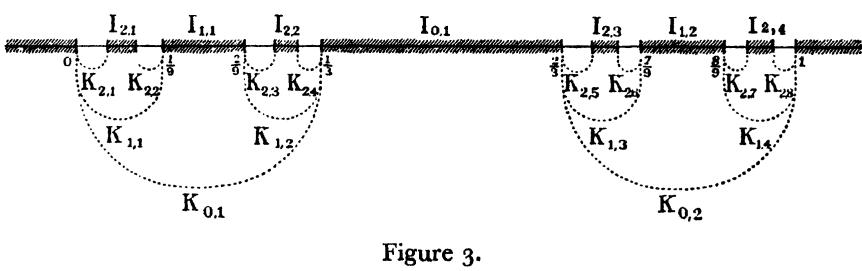
\includegraphics[keepaspectratio]{images/part002_c6c4994f.jpg}}\\
图 3。
若 \(\mathbf{K}'\) 是诸 \(\mathbf{I}_{n,p}\) 的并的余集，则闭集 \(\mathbf{K} = \mathbf{A} \cap \mathbf{K}'\) 称为 Cantor 三分集。显然 \(\mathbf{K}\) 是紧的（第 2 目，定理 2）；而且 \(\mathbf{K}\) 是全不连通的。因为若 \(\mathbf{K}\) 包含一个长度 \(>0\) 的区间 I，则 I 将含于某个区间 \(\mathbf{K}_{m,p}\) ；于是它的长度将 \(\leqslant 1/3^{m+1}\) 对每个 \(m\) 成立，这是荒谬的。

\subsection{区间到区间上的同胚}

定理 5. 设 I 是 R 中的一个区间。则 I 到 R 中的映射 f 是 I 到 \(f(I)\) 上的一个同胚，当且仅当 f 在 I 上严格单调且连续；此时 \(f(I)\) 是 R 中的一个区间。

\begin{enumerate}
\def\labelenumi{\arabic{enumi})}
\tightlist
\item
  条件是必要的。设 \(a\) 与 \(b\) 是 \(I\) 中满足 \(a < b\) 的两点，且例如设 \(f(a) < f(b)\) 。我们来证明 \(f\) 在 \(I\) 上严格递增。首先，若 \(a < c < b\) ，则必有 \(f(a) < f(c) < f(b)\) ；因为若例如有 \(f(a) < f(b) < f(c)\)
\end{enumerate}

则区间 \([a, c]\) 在 \(f\) 下的像将是一个连通集（第一章 § 11 第 2 目，命题 4），从而将包含区间 \([f(a), f(c)]\) ；于是将存在 \(x \in [a, c]\) 使得 \(f(x) = f(b)\) ，与 \(f\) 是单射的假设相矛盾。

由此推出，若 \(x\) 与 \(y\) 是 \(I\) 中满足 \(x < y\) 的任意两点，则 \(f(x) < f(y)\) ；因为 \(f(a) < f(x) < f(b)\) （当 \(a < x < b\) ），\(f(a) < f(b) < f|(x)\) （当 \(b < x\) ），且 \(f(x) < f(a) < f(b)\) （当 \(x < a\) ）；以 \(a, x, y\) 分别代替 \(a, b, x\) 重复上述论证，即见 \(f(x) < f(y)\) 。

\begin{enumerate}
\def\labelenumi{\arabic{enumi})}
\setcounter{enumi}{1}
\tightlist
\item
  条件是充分的。设 \(f\) 在 \(I\) 上连续且严格单调（比如说严格递增）：\(f(I)\) 连通，因而是区间；又因 \(f\) 严格递增，\(f\) 是 \(I\) 到 \(f(I)\) 上的一个双射。此外，\(f\) 把 \(I\) 中的每个开区间映到 \(f(I)\) 中的一个开区间，因此（§ 1 第 4 目，命题 5）\(f\) 是 \(I\) 到 \(f(I)\) 上的一个同胚。
\end{enumerate}

注. 上面证明的第一部分实际上表明，I 到 R 中的连续单射是严格单调的；因此由证明的第二部分推出，区间 I 到 R 中的每个连续单射 f 都是 I 到 \(f(\mathbf{I})\) 上的同胚。

\section{实数域}

\subsection{R 中的乘法}

有理直线 \(\mathbf{Q}\) 的拓扑不仅与加法群结构相容，而且与 \(\mathbf{Q}\) 的域结构相容。因为函数 \(xy\) 在 \((0, 0) \in \mathbf{Q} \times \mathbf{Q}\) 处连续，这是由于对每个整数 \(n > 0\) ，关系 \(|x| \leqslant 1/n\) 与 \(|y| \leqslant 1/n\) 合起来蕴含 \(|xy| \leqslant 1/n^2 \leqslant 1/n\) ；另一方面，若 \(a\) 是任一非零有理数，则函数 \(ax\) 在 \(x = 0\) 处连续，这是由于对每个整数 \(n > 0\) ，关系 \(|x| \leqslant 1/n |a|\) 蕴含 \(|ax| \leqslant 1/n\) 。这表明 \(xy\) 在 \(\mathbf{Q} \times \mathbf{Q}\) 的每一点连续（第三章 § 6 第 3 目）。

为了证明 \(1 / x\) 在 \(\mathbf{Q}^*\) 上连续，我们更精确地证明：\(1 / x\) 在 0 的任一邻域 \(\mathbf{V}\) 的余集中（关于加法结构）一致连续。即我们有 \(\left|\frac{1}{x} - \frac{1}{y}\right| = \frac{|x - y|}{xy}\) ；存在整数 \(m > 0\) ，使得 \(|x| \geqslant 1 / m\) 对每个 \(x \in \mathbb{C}\mathbf{V}\) 成立；若 \(x\) 与 \(y\) 是 \(\mathbb{C}\mathbf{V}\) 中满足 \(|x - y| \leqslant 1 / m^2 n\) 的任意两点，则将有 \(\left|\frac{1}{x} - \frac{1}{y}\right| \leqslant \frac{1}{n}\) 。

在函数 \(1 / x\) 下，\(\mathbf{Q}^*\) 上（关于加法一致结构）的任一不以 \(0\) 为聚点的 Cauchy 滤子的像是（关于加法一致结构的）一个 Cauchy 滤子。因此（第三章 § 6 第 8 目，命题 7）：

命题 1. 分别定义在 Q × Q 与 Q* 上的函数 xy 与 1/x 可以分别连续延拓到 R × R 与 R* 上，并在 R 上定义一个域结构。赋有这个结构的 R 称为实数域。

第三章 § 6 中建立的拓扑域的所有性质当然都适用；特别地，每个以实数为系数的 n 个实变量的有理函数，在其分母不为零的 \(R^{n}\) 的每一点处连续。

\subsection{乘法群 R*}

由第三章 § 6 第 7 目可知，实直线的拓扑在 \(\mathbf{R}^*\) 上诱导的拓扑与 \(\mathbf{R}^*\) 的乘法群结构相容；由于 \(\mathbf{R}^*\) 是局部紧空间 \(\mathbf{R}\) 的开子集，由此推出 \(\mathbf{R}^*\) 是局部紧拓扑群（第一章 § 9 第 7 目，命题 13），因而是完备的（第三章 § 3 第 3 目，命题 4 的推论 1；这也可由第三章 § 6 第 8 目的命题 8 得出）；当然，这后一性质涉及的是 \(\mathbf{R}^*\) 上的乘法一致结构，而不是 \(\mathbf{R}^*\) 上由 \(\mathbf{R}\) 的加法一致结构诱导的一致结构。

函数 \(xy\) 把集 \(\mathbf{Q}_{+} \times \mathbf{Q}_{+}\) 映入 \(\mathbf{Q}_{+}\) ，因此它把 \(\mathbf{R}_{+} \times \mathbf{R}_{+}\) 映入 \(\mathbf{R}_{+}\) （第一章 § 2 第 1 目，定理 1）；换句话说，两个 \(\geqslant 0\) 的实数之积 \(\geqslant 0\) 。于是公式 \((-x)y = -xy\) 与 \((-x)(-y) = xy\) 表明，一个 \(\geqslant 0\) 的数与一个 \(\leqslant 0\) 的数之积 \(\leqslant 0\) ，而两个 \(\leqslant 0\) 的数之积 \(\geqslant 0\) ；由此推出

\[
| x y | = | x |. | y |\tag{1}
\]

（它也可以由 \(\mathbf{Q} \times \mathbf{Q}\) 上相应关系的延拓得到）。

若 \(x > 0\) 且 \(y > 0\) ，我们有 \(xy \neq 0\) ，因而 \(xy > 0\) ；同样，若 \(x < 0\) 且 \(y > 0\) ，则 \(xy < 0\) ；若 \(x < 0\) 且 \(y < 0\) ，则 \(xy > 0\) 。特别地，若 \(x \neq 0\) ，我们有 \(x^2 > 0\) ，因此实数的平方和除非每个数都为零，否则不可能为零。

若 \(x > 0\) 且 \(y \leqslant z\) （相应地 \(y < z\) ），我们有 \(xy \leqslant xz\) （相应地 \(xy < xz\) ）；换句话说，比率 \(> 0\) 的位似保持 \(\mathbf{R}\) 上的次序。由于 \((-x)y = -xy\) ，比率 \(< 0\) 的位似把 \(\mathbf{R}\) 上的序变为反序。

若 \(x > 0\) ，我们有 \(\mathbf{1} / x > 0\) ，因为 \(x.(\mathbf{1} / x) = \mathbf{1} > 0\) 。若 \(0 < x < y\) ，我们有 \(xy > 0\) ，于是 \(x.(\mathbf{1} / xy) < y.(\mathbf{1} / xy)\) ，即 \(\mathbf{1} / y < \mathbf{1} / x\) 。因此，映射 \(x \to \mathbf{1} / x\) 把集 \(\mathbb{R}_+^*\) （即 \(> 0\) 的实数组成的集）映到其自身上，它是严格递减的。

我们同样看出，函数 \(\mathbf{1} / x\) 在 \(] \leftarrow, o[, \text{ 且因此函数 } \frac{\mathbf{1}}{x - a}\) 在区间 \(] \leftarrow, a[ \text{ 与 } ]a, \rightarrow [.\) 的每一个内严格递减。

由上文推出，\(R_{+}^{*}\) 是乘法群 \(R^{*}\) 的一个子群；而且，序关系 \(x \leqslant y\) 与 \(R_{+}^{*}\) 的乘法群结构相容；换句话说，\(R_{+}^{*}\) 是一个全序群。

两个 \(\geqslant0\) 的实数之积 \(\geqslant0\) 这一事实可以表述为：R 是一个有序域；上述所有性质对一切有序域都成立。

命题 2. 乘法群 \(\mathbf{R}^{*}\) （ \(\neq 0\) 的实数组成的）是一个拓扑群，同构于它的子群 \(\mathbf{R}_{+}^{*}\) 与 \(\mathbf{U}_{0}\) 的积，其中

\[
\mathrm{U} _ {0} = \{- 1, + 1 \}.
\]

对每个 \(x \neq 0\) ，令 \(\operatorname{sgn} x\) 表示 \(\frac{x}{|x|}\) （ \(x\) 的符号）。函数 \(\operatorname{sgn}\) 是 \(\mathbf{R}^*\) 到 \(U_0\) 上的一个同态。我们有 \(x = |x| \operatorname{sgn} x\) ，且 \(x\) 的这个表成 \(\mathbf{R}_+^*\) 的一个元素与 \(U_0\) 的一个元素之积的分解是唯一的；因而 \(\mathbf{R}^*\) 的群结构是 \(\mathbf{R}_+^*\) 与 \(U_0\) 的群结构之积。另一方面，映射 \(x \to |x|\) 连续，且 \(x \to \operatorname{sgn} x = \frac{x}{|x|}\) 也连续，因为 \(x \neq 0\) 。由此即得结论。

我们通过令 sgn o = o 把函数 sgn 延拓到整个 R。

我们将在第五章（§ 4 第 1 目，定理 1）看到，拓扑群 \(\mathbf{R}_{+}^{*}\) 同构于加法群 \(\mathbf{R}\) ；这将完成对拓扑群 \(\mathbf{R}^{*}\) 的结构的确定。

\subsection{n 次根}

设 \(n\) 是任一整数 \(> 0\) 。由关系 \(0 < x < y\) ，对 \(n\) 用归纳法推出 \(0 < x^n < y^n\) 。换句话说，函数 \(x \to x^n\) 对 \(x \geqslant 0\) 严格递增；它显然在每一点连续，因此（§ 2 第 6 目，定理 5）是 \(\mathbf{R}_{+}\) 到一个区间 \(\mathbf{I}\) 上的同胚。另一方面，由于 \(x \geqslant 1\) 蕴含 \(x^{n-1} \geqslant 1\) ，从而 \(x^n \geqslant x\) ，可见 \(\mathbf{I}\) 不是有界的，因而 \(\mathbf{I} = \mathbf{R}_{+}\) 。对于 \(x \geqslant 0\) ，映射 \(x \to x^n\) 的逆的值记作 \(x^{1/n}\) 或 \(\sqrt[n]{x}\) ，称为 \(x\) 的 \(1\) 次幂或 \(x\) 的 n 次根（当 \(n = 2\) , 3 时，我们说平方根、立方根；当 \(n = 2\) 时，我们用 \(\sqrt{x}\) 代替 \(\sqrt[2]{x}\) 书写）。正数 \(x^{1/n}\) 于是定义为方程的唯一正解

\[
y ^ {n} = x \quad (x \geqslant 0).\tag{2}
\]

特别地，我们看到存在实数 x 使得 \(x^{2}=2\) ，而没有有理数具有这一性质；这样我们重新得到有理直线 Q 不是完备空间这一事实。

映射 \(x \to x^{1/n}\) （ \(\mathbf{R}_+\) 到其自身的）严格递增且连续。由 (2) 我们有 \(0^{1/n}=0, 1^{1/n}=1\) ，还有

\[
(x y) ^ {1 / n} = x ^ {1 / n} y ^ {1 / n};\tag{3}
\]

因而 \(x \to x^{1/n}\) 是拓扑群 \(\mathbf{R}_{+}^{*}\) 的一个自同构。

在第五章 § 4 第 1 目中，我们将通过求出乘法群 \(\mathbf{R}_{+}^{*}\) 的所有自同构来推广这一结果。

\section{扩充实直线}

\subsection{R 的开区间之间的同胚}

命题 1. \(\mathbf{R}\) 的所有非空开区间都同胚于 \(\mathbf{R}\) 。先考察有界开区间 \(\mathbf{I} = ]a\) , \(b[(a < b)\) 。对每个 \(x \in \mathbf{I}\) ，令 \(f(x) = -\left(\frac{1}{x - a} + \frac{1}{x - b}\right)\) 。这个函数在 \(\mathbf{I}\) 上连续且严格递增，因为我们已看到 \(\frac{1}{x - b}\) 在 \(]\leftarrow, b[\) 中严格递减，而 \(\frac{1}{x - a}\) 在 \(]a, \rightarrow[\) 中严格递减。由此推出 \(f\) 是 \(\mathbf{I}\) 到一个区间 \(f(\mathbf{I})\) （ \(\mathbf{R}\) 中的）上的同胚（ \(\S 2\) 第 6 目，定理 5）。\(f(\mathbf{I})\) 既不上有界也不下有界；因为若例如 \(f(x) \leqslant c\) 对所有 \(x \in \mathbf{I}\) 成立，则将得出 \(1 - \frac{b - x}{x - a} \leqslant c(b - x)\) （因为 \(b - x > 0\) ）；而当 \(x\) 充分接近 \(b\) 时这就导致矛盾（利用不等式两边这两个有理函数在点 \(b\) 处的连续性）。因而 \(f(\mathbf{I}) = \mathbf{R}\) ，从而每个有界开区间都同胚于 \(\mathbf{R}\) 。设 \(g\) 为 \(f\) 的逆：它把 \(\mathbf{R}\) 的每个无界开区间映到一个区间 \(J\) （含于 \(I\) 且在 \(I\) 中开的）上。由于 \(I\) 在 \(\mathbf{R}\) 中开，\(J\) 在 \(\mathbf{R}\) 中也开；由于它有界，它同胚于 \(\mathbf{R}\) ；这样我们就证明了每个无界开区间都同胚于 \(\mathbf{R}\) 。

注. 为了证明所有有界开区间彼此同胚，只需注意：若 \(a \neq b\) 且 \(a' \neq b'\) ，则存在 R 到其自身的一个形如 \(x \to \alpha x + \beta\) 的同胚（且只有一个），它把 a 映到 \(a'\) ，把 b 映到 \(b'\) ，从而把以 a, b 为端点的开（相应地半开、闭）区间映到以 \(a', b'\) 为端点的开（相应地半开、闭）区间；读者通过计算 \(\alpha\) 与 \(\beta\) 容易验证这一点。

\subsection{扩张直线}

我们现在要通过给 R 添加两个新元素来定义一个拓扑空间 \(\overline{R}\) ，使得 R 到 R 的有界开区间 I 上的每个同胚都能延拓为 \(\overline{R}\) 到与 I 有相同端点的闭区间上的同胚。

设 \(\overline{\mathbf{R}}\) 是由（集合论， R, § 4 第 5 目）向 \(\mathbf{R}\) 添加两个新元素得到的集，这两个新元素记作 \(-\infty\) 与 \(+\infty\) 。我们通过把 \(\mathbf{R}\) 上的序延拓到 \(\overline{\mathbf{R}}\) ，方式是令 \(-\infty < a\) 与 \(a < +\infty\) （对所有 \(a \in \mathbf{R}\) ）以及 \(-\infty < +\infty\) ；显然我们如此得到一个全序集，其序在 \(\mathbf{R}\) 上诱导出实直线的序。其次，考察 \(\overline{\mathbf{R}}\) 上由 \(\overline{\mathbf{R}}\) 的开区间全体所生成的拓扑。由于在 \(\mathbf{R}\) 上 \(\overline{\mathbf{R}}\) 的开区间的迹是 \(\mathbf{R}\) 的开区间，这个拓扑在 \(\mathbf{R}\) 上诱导出实直线的拓扑。

定义 1. 赋有上述序结构与拓扑的集合 \(\overline{\mathbf{R}}\) 称为扩充实直线。

在使用扩张直线 \(\overline{\mathbf{R}}\) 时，出于用语习惯，把它的点称为实数往往是方便的；这时 \(\mathbf{R}\) 的点称为有限实数。我们在本节及本章随后三节中采用这一约定；今后凡采用这一约定时，我们都会明确指出它适用于正文的哪一部分。

若 \(a\) 是有限实数，则区间 \([a, +\infty[ \text{ 与 } ] - \infty, a]\) （相应地 \(]a, +\infty[ \text{ 与 } ] - \infty, a[\) ）（ \(\overline{\mathbf{R}}\) 中的）含于 \(\mathbf{R}\) ，且与 \(\mathbf{R}\) 中迄今记作 \([a, \rightarrow[ \text{ 与 } ] \leftarrow, a]\) （相应地 \(]a, \rightarrow[ \text{ 与 } ] \leftarrow, a[\) ）的区间一致；这个新记号用得远为频繁。再者，\(\mathbf{R}\) 与区间 \(] - \infty, +\infty[ \text{ 位于 } \overline{\mathbf{R}}, \text{ 且有时也如此记之。}\)

命题 2. 每个同胚 \(f\) （ \(\mathbf{R}\) 到区间 \(]a, b[\) 上的）都可以延拓为同胚 \(\overline{f}\) （ \(\overline{\mathbf{R}}\) 到 \([a, b]\) 上的）。若 \(f\) 是递增函数，则 \(\overline{f}\) 是 \(\overline{\mathbf{R}}\) 到 \([a, b]\) 上的一个序同构。

设 \(f\) 是递增同胚。若把 \(f\) 延拓到 \(\mathbf{R}\) ，方式是令 \(\overline{f}(-\infty) = a\) 与 \(\overline{f}(+\infty) = b\) ，则显然 \(\overline{f}\) 是 \(\overline{\mathbf{R}}\) 到 \([a, b]\) 上的严格递增映射（因而是双射）。于是 \(\overline{f}\) 把 \(\overline{\mathbf{R}}\) 的每个开区间映到关于 \([a, b]\) 为开的一个区间，因而由 § 1 第 4 目的定义 1 与命题 5，它是 \(\overline{\mathbf{R}}\) 到 \([a, b]\) 上的同胚。

若 \(f\) 递减，则对递增同胚 \(x \to -f(x)\) （ \(\mathbf{R}\) 到 \(] - b, - a[\) 上的）应用已证的结果。

因此，§ 2 中得到的区间 \([a, b]\) 的所有只涉及区间的序结构与拓扑的性质都可以搬到 \(\overline{R}\) 上；于是有下列命题：

命题 3. 扩充实直线是紧的。

因此（第二章 § 4 第 1 目，定理 1）在 \(\overline{\mathbf{R}}\) 上存在唯一一个与其拓扑相容的一致结构；这个一致结构同构于在 \([a, b]\) 上由 \(\mathbf{R}\) 的加法一致结构诱导的一致结构。但应当注意，在 \(\mathbf{R}\) 上由 \(\overline{\mathbf{R}}\) 的一致结构诱导的一致结构不是 \(\mathbf{R}\) 的加法一致结构（尽管它与实直线的拓扑相容）；因为 \(\mathbf{R}\) 关于其加法一致结构是完备空间，却不是 \(\overline{\mathbf{R}}\) 的完备子空间，因为它在 \(\overline{\mathbf{R}}\) 中不闭。

命题 4. \(\overline{\mathbf{R}}\) 的每个非空子集都有上确界与下确界。

R 的非空子集 A 的上确界（相应地下确界）记作 sup A（相应地 inf A）。显然

\[
\inf A \leqslant \sup A.\tag{1}
\]

若 \(\mathbf{A} \subset \mathbf{B}\) ，则 \(\sup \mathbf{A} \leqslant \sup \mathbf{B}\) 且 \(\inf \mathbf{A} \geqslant \inf \mathbf{B}\) （集合论，第三章 § 1 第 9 目，命题 4）。

命题 5. \(\overline{R}\) 的子集 A 连通当且仅当 A 是区间。

推论. 扩充实直线是连通的、局部连通的空间。

命题 6. 映射 \(f\) （区间 \(I\) （ \(\overline{R}\) 的）到 \(\overline{R}\) 中的）是 \(I\) 到 \(f(I)\) 上的同胚，当且仅当 \(f\) 在 \(I\) 上严格单调且连续；此时 \(f(I)\) 是 \(\overline{R}\) 的一个区间。

最后，函数 \(\sup (x,y)\) 与 \(\inf (x,y)\) 在 \(\overline{\mathbf{R}}\times \overline{\mathbf{R}}\) 上连续

\subsection{\texorpdfstring{\(\bar{R}\) 中的加法与乘法}{\textbackslash bar\{R\} 中的加法与乘法}}

首先注意，函数 \(-x\) 可以连续延拓到 \(\overline{\mathbf{R}}\) ，依照公式 \(-(-\infty)=+\infty\) 与 \(-(+\infty)=-\infty\) ；如此延拓后的函数是 \(\overline{\mathbf{R}}\) 到其自身的一个同胚。

其次，考察函数 \(x + y\) 与 xy，它们定义在 \(R \times R\) 上、取值于 R 中；通过认为它们取值于拓扑空间 \(\overline{R}\) ，我们将看到它们也能在 \(\overline{R} \times \overline{R}\) 的某些点连续延拓。

就 \(x + y\) 而言，令 \(A' = ] - \infty, + \infty]\) 与 \(A'' = [-\infty, + \infty[\) 。于是有下述命题：

命题 7. 函数 \(x + y\) 可以依照公式连续延拓到集 \(\mathbf{A}' \times \mathbf{A}'\) 与 \(\mathbf{A}'' \times \mathbf{A}''\) 的每一个上，公式为

\[
\left\{ \begin{array}{l l} x + (+ \infty) = (+ \infty) + x = + \infty & (x \neq - \infty), \\ x + (- \infty) = (- \infty) + x = - \infty & (x \neq + \infty). \end{array} \right.\tag{2}
\]

例如我们证明：当 \((x,y)\) 趋于点 \((a,+\infty)\) \((a\neq-\infty)\) 而保持属于 \(R\times R\) 时，\(x+y\) 趋于 \(+\infty\) 。存在有限数 b\textless a ，而区间 {]}b, \(+\infty\) {[} 是 a 在 R 中的邻域；对任意有限 c ，关系 x\textgreater b 与 y\textgreater c-b 蕴含 \(x+y>c\) ，这表明 \(x+y\) 可以任意接近 \(+\infty\) ，只要 \((x,y)\) 充分接近 \((a,+\infty)\) 。其他情形论证类似。

相反，\(x + y\) 在点 \((-\infty, +\infty)\) 与 \((+\infty, -\infty)\) （ \(\overline{\mathbf{R}} \times \overline{\mathbf{R}}\) 的）处没有极限。因为若 \(x + y\) 有极限 \(k\) （有限或无限），当 \((x, y)\) 趋于 \((+\infty, -\infty)\) 而保持属于 \(\mathbf{R} \times \mathbf{R}\) 时，则将推出：对每个有限 \(a\) ，函数 \((x + a) - x\) 将趋于 \(k\) ，当 \(x\) 趋于 \(+\infty\) 而保持属于 \(\mathbf{R}\) 时；而这是荒谬的，因为 \((x + a) - x = a\) 且 \(a\) 是任意的。

函数 \(x + y\) 把 \(A' \times A'\) （相应地 \(A'' \times A''\) ）映入 \(A'\) （相应地 \(A''\) ）。因此它是 \(A'\) （相应地 \(A''\) ）上的一个合成法则，它延拓了 \(R\) 上的加法法则。由恒等延拓原理（第一章 § 8 第 1 目，命题 2 的推论 1），这个法则交换且结合； o 是这个法则的单位元素；而由公式 (2)，\(A'\) 的唯一非正则元素（代数，第一章 § 2 第 2 目）是 \(+\infty\) 。

若 \(x, y, z, t\) 是 \(\overline{\mathbf{R}}\) 中满足 \(x \leqslant y\) 与 \(z \leqslant t\) 的点，则只要不等式两边都有定义，就有 \(x + z \leqslant y + t\) 。

注意在 \(\overline{\mathbf{R}}\) 中，由公式 (2)，关系 \(x < y\) 蕴含 \(x + z < y + z\) 仅当 \(z\) 有限时；容易验证，只要不等式两边都有定义，关系 \(x < y\) 与 \(z < t\) 就蕴含 \(x + z < y + t\) 。

在 \(\overline{\mathbf{R}}\) 中我们令 \(x^{+} = \sup (x,0)\) ，\(x^{-} = \sup (-x,0)\) ，\(|x| = \sup (x, - x)\) ；于是 \((+\infty)^{+} = (-\infty)^{-} = +\infty\) 且 \((+\infty)^{-} = (-\infty)^{+} = 0\) ，而 \(|+\infty| = |- \infty| = +\infty\) 。和 \(x^{+} - x^{-}\) 与 \(x^{+} + x^{-}\) 对所有 \(x \in \overline{\mathbf{R}}\) 有定义，因而由恒等延拓原理分别等于 \(x\) 与 \(|x|\) 。同样，只要和 \(x + y\) 有定义，我们就有 \(|x + y| \leqslant |x| + |y|\) 。

相反要注意，§ 1 第 1 目的公式 (6) 与 (7) 对某些值 \(x\) 与 \(y\) （ \(\overline{\mathbf{R}}\) 中的）可能不再有意义；例如，若 \(x = -\infty\) 且 \(y = 0\) ，我们有 \(\sup (x, y) = 0\) ，但和 \(x + (y - x)^+\) 没有定义，因为 \((y - x)^+ = +\infty\) 。

令 \(\overline{\mathbf{R}}^{*}\) 表示 \(o\) 在 \(\overline{\mathbf{R}}\) 中的余集。于是乘法情形的命题 7 的类似命题如下：

命题 8. 函数 \(xy\) 可以依照公式连续延拓到集 \(\overline{\mathbf{R}}^* \times \overline{\mathbf{R}}^*\) 上，公式为

\[
\left\{ \begin{array}{l} x. (+ \infty) = (+ \infty). x = \left\{ \begin{array}{l l} + \infty & \text {if} \quad x > 0 \\ - \infty & \text {if} \quad x <   0 \end{array} \right. \\ x. (- \infty) = (- \infty). x = \left\{ \begin{array}{l l} - \infty & \text {if} \quad x > 0 \\ + \infty & \text {if} \quad x <   0. \end{array} \right. \end{array} \right.\tag{3}
\]

我们把证明留给读者；它与命题 7 的证明类似。

同样，我们看到 \(xy\) 在点 \((0, +\infty), (+\infty, 0), (0, -\infty), (-\infty, 0)\) （ \(\overline{\mathbf{R}} \times \overline{\mathbf{R}}\) 的）处没有极限。

函数 \(xy\) 是 \(\overline{\mathbf{R}}^*\) 上的一个合成法则，它延拓了 \(\mathbf{R}\) 上的乘法法则；这个法则结合且交换（恒等延拓原理）；它以 1 为单位元素；而 \(\overline{\mathbf{R}}^*\) 中的非正则元素是 \(+\infty\) 与 \(-\infty\) 。

若 \(x \leqslant y\) 且 \(z > 0\) ，则只要不等式两边都有定义，就有 \(xz \leqslant yz\) 。若积 \(xy\) 有定义，则 \(|x| \cdot |y|\) 也有定义，且我们有 \(|xy| = |x| \cdot |y|\) 。

最后，分配律公式

\[
x (y + z) = x y + x z\tag{4}
\]

只要出现在两边的所有运算都有定义，它由恒等延拓原理仍然有效。

\pandocbounded{
\includegraphics[keepaspectratio]{images/part002_cca5eabe.jpg}}

注意可能发生 (4) 的左边有定义而右边没有定义的情形：例如考察 \(x = +\infty\) ， y = 2 与 z = -1 的情形。因此在 R 中使用分配律公式应当谨慎。

\section{实值函数}

\subsection{实值函数}

定义 1. 一个集 X 到实直线中的映射称为定义在 X 上的实值函数（或实函数）。

通过与 § 4 第 2 目所述类似的用语习惯，X 到 \(\overline{\mathbf{R}}\) 中的映射在本节及下一节中也称为定义在 X 上的实值函数。X 到 \(\mathbf{R}\) 中的映射将称为有限实值函数。

若 \(f\) 与 \(g\) 是定义在 \(\mathbf{X}\) 上的两个实值函数，则关系 \(f \leqslant g\) 依定义等价于“\(f(x) \leqslant g(x)\) 对所有 \(x \in \mathbf{X}\) 成立；”这个关系是集 \(\overline{\mathbf{R}}^{\mathbf{X}}\) （ \(\mathbf{X}\) 上所有实值函数的）上的一个序。由这个关系排序的集 \(\overline{\mathbf{R}}^{\mathbf{X}}\) 是一个格；因为若 \(f\) 与 \(g\) 是任意两个实值函数，则函数 \(h\) 由 \(h(x) = \sup (f(x), g(x))\) （对所有 \(x \in \mathbf{X}\) ）所定义，它是 \(\mathbf{X}\) 上既 \(\geqslant f\) 又 \(\geqslant g\) 的实值函数中的最小者；按照一般记号，我们把这个函数（即 \(f\) 与 \(g\) 在 \(\overline{\mathbf{R}}^{\mathbf{X}}\) 中的上确界）记作 \(\sup (f, g)\) 。类似地，在每个 \(x \in \mathbf{X}\) 处取值 \(\inf (f(x), g(x))\) 的函数记作 \(\inf (f, g)\) 。

注意 sup \((f, g)\) 是映射

\[
(u, v) \mapsto \sup (u, v)
\]

\(\overline{\mathbf{R}}\times \overline{\mathbf{R}}\) 到 \(\overline{\mathbf{R}}\) 中的映射与映射 \(x\to (f(x),g(x))\) （ \(\mathbf{X}\) 到 \(\overline{\mathbf{R}}\times \overline{\mathbf{R}}\) 中的）的复合。inf \((f,g)\) 亦然。

实值函数 \(f\) （定义在集 \(\mathbf{X}\) 上的）称为在 \(\mathbf{X}\) 中上有界（相应地下有界）的，如果 \(f(\mathbf{X})\) 是 \(\mathbf{A}'' = [-\infty, +\infty[\) 的子集且上有界（相应地，如果 \(f(\mathbf{X})\) 是 \(\mathbf{A}' = ] - \infty, +\infty]\) 的子集且下有界）。\(f\) 称为在 \(\mathbf{X}\) 中有界的，如果它既上有界又下有界，也就是说 \(f(\mathbf{X})\) 是 \(\mathbf{R}\) 的有界子集。

因此每个有界函数都是有限的。其逆不真，例如函数 \(\mathbf{1} / x\) （在 \(\mathbb{R}_+^* = ]0, +\infty[\) 上）所示。
% semantic-fragments: legacy-input-seam
\relax{}
\subsection{滤子化集合上定义的实值函数}

命题 1. 设 \(f\) 与 \(g\) 是定义在集合 \(\mathbf{X}\) （它由滤子 \(\mathfrak{F}\) 滤子化）上的两个实值函数。若 \(\lim_{\mathfrak{F}} f\) 与 \(\lim_{\mathfrak{F}} g\) 存在，且对每个子集 \(\mathbf{A} \in \mathfrak{F}\) 存在 \(x \in \mathbf{A}\) 使得 \(f(x) \leqslant g(x)\) ，则我们有 \(\lim_{\mathfrak{F}} f \leqslant \lim_{\mathfrak{F}} g\) 。

为证明这一结果，我们将证明下述等价的命题：

命题 2. 设 \(f\) 与 \(g\) 是定义在集合 \(X\) （它由滤子 \(\mathfrak{F}\) 滤子化）上的两个实值函数。若 \(\lim_{\mathfrak{F}} f\) 与 \(\lim_{\mathfrak{F}} g\) 存在，且 \(\lim_{\mathfrak{F}} f > \lim_{\mathfrak{F}} g\) ，则存在一个集 \(A \in \mathfrak{F}\) ，使得 \(f(x) > g(x)\) 对一切 \(x \in A\) 成立。

设 \(a = \lim_{\mathfrak{F}} f\) ，设 \(b = \lim_{\mathfrak{F}} g\) ，并设 \(c\) 满足 \(b < c < a\) 。区间 \(]c, +\infty]\) （属于 \(\overline{\mathbf{R}}\) ）（相应地，\([-\infty, c[)\) ）是 \(a\) （相应地，\(b\) ）的邻域；因此存在一个集 \(M \in \mathfrak{F}\) （相应地，一个集 \(N \in \mathfrak{F}\) ），使得 \(f(x) > c\) 对一切 \(x \in M\) 成立{[}相应地，\(g(x) < c\) 对一切 \(x \in N\) 成立{]}。集 \(A = M \cap N\) 属于 \(\mathfrak{F}\) ，且 \(f(x) > c > g(x)\) 对一切 \(x \in A\) 成立。

作为命题 1 的一个特例，我们有下述定理：

定理 1（不等式延拓原理）. 设 \(f\) 与 \(g\) 是定义在集合 \(\mathbf{X}\) （它由滤子 \(\mathfrak{F}\) 滤子化）上的两个实值函数。若 \(\lim_{\mathfrak{F}} f\) 与 \(\lim_{\mathfrak{F}} g\) 存在，且 \(f \leqslant g\) ，则 \(\lim_{\mathfrak{F}} f \leqslant \lim_{\mathfrak{F}} g\) 。

\pandocbounded{
\includegraphics[keepaspectratio]{images/part002_67e89114.jpg}}

注. 特别地，若 \(f(x) < g(x)\) 对一切 \(x \in X\) 成立（或者只对滤子 \(\overline{\mathbf{R}}\) 的某一个集中的各点成立），则由定理 1 可以推出 \(\lim_{\mathfrak{F}} f \leqslant \lim_{\mathfrak{F}} g\) ；但我们不能推出严格不等式 \(\lim_{\mathfrak{F}} f < \lim_{\mathfrak{F}} g\) 。例如，取 \(X\) 为自然数集 \(N\) ，赋以 Fréchet 滤子，且设 \(f(n) = 0\) ，\(g(n) = 1/n\) ，则 \(f(n) < g(n)\) 对一切 \(n\) 成立，但 \(\lim_{n \to \infty} f(n) = \lim_{n \to \infty} f(n) = 0\) 。因此，在严格不等式中过渡到极限时，严格性会丢失。

定理 2（单调极限定理）. 设 X 是一个有序集，A 是 X 的一个有向子集 (*)。每个定义在 A 上的单调实值函数 f 关于 A 都有极限（第一章，§ 7，第 3 节）；若 f 递增（相应地，递减），则此极限等于集 \(f(A) \subset \overline{\mathbf{R}}\) 的上确界（相应地，下确界）。

例如设 \(f\) 递增，并令 \(a = \sup f(A)\) 。若 \(a = -\infty\) ，定理是平凡的。若 \(a > -\infty\) ，则对每个 \(b < a\) 存在 \(x \in A\) 使得 \(b < f(x) \leqslant a\) ；于是，若 \(S_x\) 是 \(A\) 的相对于 \(x\) 的截面（即所有 \(y \geqslant x\) 所成之集，参看第一章，§ 6，第 3 节），则 \(f(S_x)\) 含于 \(]b, +\infty]\) （它是 \(a\) 的一个邻域）之中，定理得证。若 \(f\) 递减，证明类似。

推论. 定义在有序集 X 的有向子集 A 上的递增（相应地，递减）实值函数，关于 A 有有限极限的充分必要条件是它在 A 中上有界（相应地，下有界）。

若把定理 2 应用于 \(\mathbf{A} = \mathbf{X} = \mathbf{N}\) （按关系 \(\leqslant\) 定序）的情形，就得到下述命题：

命题 3. 每个实数单调序列在 R 中有极限。特别地，由有限数组成的递增（相应地，递减）序列，当其上有界（相应地，下有界）时收敛于一个有限实数，否则收敛于 +∞（相应地，-∞）。例如，正整数序列收敛于 +∞。

这一事实正是用记号 \(\lim_{n\to \infty}u_n\) 表示序列极限的由来（第一章，§ 7，第 3 节）。

同样，每个严格递增的整数序列 \((p_n)\) 收敛于 \(+\infty\) ；因为由归纳法可见，\(p_n \geqslant p_0 + n\) 对一切 \(n\) 成立。

\subsection{实变量函数的右极限与左极限}

设 A 是 \(\overline{R}\) 的一个非空子集，且设 \(a \neq -\infty\) 是 \(\overline{R}\) 中位于集 \(B = A \cap [-\infty, a[\) 的闭包中的一点。集 B 关于关系 \(\leqslant\) 有向，它的截面滤子 F 与 a 在 \(\overline{R}\) 中的邻域滤子在 B 上的迹相同。

定义 2. 设 \(f\) 是定义在一个非空子集 \(A\) （属于 \(\overline{\mathbf{R}}\) ）上、取值于一个拓扑空间 \(X\) 中的函数。\(f\) 关于滤子 \(\mathfrak{F}\) 的极限（若存在）称为 \(f\) 在点 \(a\) 处关于 \(A\) 的左极限，记作

\(\lim_{x \to a, x < a, x \in \mathbf{A}} f(x), \text{ 或 } f(a - ), \text{ 若 } \mathbf{X} \text{ 是 Hausdorff 的。}\)

同样，若 \(a\) 位于集 \(A \cap ]a, +\infty]\) 的闭包中，我们定义 \(f\) 在点 \(a\) 处的右极限（若存在），并把它记作 \(\lim_{x \to a, x > a, x \in A} f(x)\) ，或 \(f(a+)\) ，如果 \(X\) 是豪斯多夫的。

下述命题是定理 2 的一个直接推论：

命题 4. 设 A 是 \(\overline{\mathbf{R}}\) 的一个子集，且设 \(a \neq -\infty\) 是交集 \(\mathbf{A} \cap [-\infty, a[\) 的闭包中的一点。若 \(f\) 是定义在 A 上的单调实值函数，则 \(f\) 有左极限 \(f(a - )\) （在 \(a\) 处且关于 A ）。

\subsection{实值函数的界}

定义 3. 设 \(f\) 是定义在集合 \(\mathbf{X}\) 上的实值函数，\(\mathbf{A}\) 是 \(\mathbf{X}\) 的一个非空子集。此时集 \(f(\mathbf{A})\) 在 \(\overline{\mathbf{R}}\) 中的上确界（相应地，下确界）称为 \(f\) 在 \(\mathbf{A}\) 中的上确界（相应地，下确界），记作 \(\sup_{x\in \mathbf{A}}f(x)\left[\text{resp. } \inf_{x\in \mathbf{A}} f(x)\right]\) 。

特别地，若 A 是 \(\overline{R}\) 的一个非空子集，则

\[
\sup \mathrm{A} = \sup _ {x \in \mathrm{A}} x.\tag{1}
\]

用右端的记号来表示 A 的上确界，往往更为方便。

数 \(a = \sup_{x \in \mathbf{A}} f(x)\) 由下列两条性质刻画：

\begin{enumerate}
\def\labelenumi{(\roman{enumi})}
\item
  对一切 \(x \in \mathbf{A}, f(x) \leqslant a\) 。
\item
  对每个 \(b < a\) ，存在 \(x \in \mathbf{A}\) 使得 \(b < f(x) \leqslant a\) 。
\end{enumerate}

数 \(\sup_{x\in\mathbf{A}}f(x)\) 与 \(\inf_{x\in\mathbf{A}}f(x)\) 属于 \(f(\mathbf{A})\) 在 \(\overline{\mathbf{R}}\) 中的闭包。我们有 \(\inf_{x\in\mathbf{A}}f(x)\leqslant\sup_{x\in\mathbf{A}}f(x)\) ；且这两个数相等当且仅当 \(f\) 在 \(\mathbf{A}\) 上取常值。

定义在集合 X 上的实值函数在 X 的一个非空子集 A 中上有界（相应地，下有界）当且仅当 \(\sup_{x\in\mathbf{A}}f(x)<+\infty\) {[}相应地，\(\inf_{x\in\mathbf{A}}f(x)>-\infty\) {]}。f 在 A 中有界当且仅当 \(|f|\) 在 A 中上有界，亦即当且仅当 \(\sup_{x\in\mathbf{A}}|f(x)|<+\infty\) 。

我们有

\[
\inf _ {x \in \mathbf {A}} f (x) = - \sup _ {x \in \mathbf {A}} (- f (x)).\tag{2}
\]

这一关系式把下确界的所有性质都化归为上确界的性质；因此在一般情况下我们只谈论后者。

命题 5. 设 \(f\) 是定义在集合 \(\mathbf{X}\) 上的一个实值函数。在集 \(\mathfrak{F}(\mathbf{X})\) （由 \(\mathbf{X}\) 的所有有限子集组成，按关系 \(\subset\) 有向）上，实值函数 \(\mathbf{H} \to \sup_{x \in \mathbf{H}} f(x)\) 是递增的，实值函数 \(\mathbf{H} \to \inf_{x \in \mathbf{H}} f(x)\) 是递减的，并且我们有

\[
\left\{ \begin{array}{l} \sup _ {x \in \mathbf {A}} f (x) = \lim _ {\mathbf {H} \in \mathfrak {F} (\mathbf {X})} (\sup _ {x \in \mathbf {H}} f (x)), \\ \inf _ {x \in \mathbf {A}} f (x) = \lim _ {\mathbf {H} \in \mathfrak {F} (\mathbf {X})} (\inf _ {x \in \mathbf {H}} f (x)). \end{array} \right.\tag{3}
\]

设 \(\varphi(\mathbf{H}) = \sup_{x \in \mathbf{H}} f(x)\) 。显然 \(\varphi\) 递增，因而有极限 \(a\) （第 2 节，定理 2）；又因对一切 H 有 \(\varphi(\mathbf{H}) \leqslant \sup_{x \in \mathbf{A}} f(x)\) ，故有 \(a \leqslant \sup_{x \in \mathbf{A}} f(x)\) （第 2 节，定理 1）。倘若 \(a < \sup_{x \in \mathbf{A}} f(x)\) ，就会存在 \(x_0 \in \mathbf{X}\) 使得 \(a < f(x_0)\) ；但这是矛盾的，因为 \(\varphi(\mathbf{H}) \geqslant f(x_0)\) （只要 \(x_0 \in \mathbf{H}\) ）。

特别地，由 (1)，若 A 是 \(\overline{R}\) 的任意一个非空子集，则我们有

\[
\sup \mathrm{A} = \lim _ {\mathrm{H} \in \mathfrak {F} (\mathrm{A})} (\sup _ {x \in \mathrm{H}} x).\tag{4}
\]

命题 6. 设 \(f\) 与 \(g\) 是定义在 \(\mathbf{X}\) 上的两个实值函数。若 \(f(x) \leqslant g(x)\) 对每一点 \(x\) （属于某个非空子集 \(A\) ，而该子集含于 \(\mathbf{X}\) ）成立，则我们有

\[
\left\{ \begin{array}{l} \sup _ {x \in \mathbf {A}} f (x) \leqslant \sup _ {x \in \mathbf {A}} g (x), \\ \inf _ {x \in \mathbf {A}} f (x) \leqslant \inf _ {x \in \mathbf {A}} g (x). \end{array} \right.\tag{5}
\]

命题 7. 设 \(f\) 是定义在 \(\mathbf{X}\) 上的一个实值函数。若 \(\mathbf{A}\) 与 \(\mathbf{B}\) 是 \(\mathbf{X}\) 的两个非空子集，且 \(\mathbf{A} \subset \mathbf{B}\) ，则

\[
\sup _ {x \in \mathbf {A}} f (x) \leqslant \sup _ {x \in \mathbf {B}} f (x).\tag{6}
\]

命题 8. 设 \(f\) 是定义在 \(\mathbf{X}\) 上的一个实值函数，且设 \((\mathbf{A}_t)_{t \in I}\) 是由 \(\mathbf{X}\) 的非空子集组成的一个非空族；则

\[
\sup_{x\in \bigcup_{t\in \mathbf{I}}\mathbf{A}_{t}}f(x) = \sup_{t\in \mathbf{I}}(\sup_{x\in \mathbf{A}_{t}}f(x)).\tag{7}
\]

设 \(f\) 是定义在乘积集合 \(\mathbf{X}_1 \times \mathbf{X}_2\) 上的一个实值函数。若 \(\mathbf{A}_2\) 是 \(\mathbf{X}_2\) 的一个非空子集，我们用 \(\sup_{x_2 \in \mathbf{A}_2} f(x_1, x_2)\) 表示在 \(\mathbf{A}_2\) 中取的上确界，即实值函数 \(x_2 \to f(x_1, x_2)\) （定义在 \(\mathbf{X}_2\) 上）的上确界。由命题 8 我们特别推出：

命题 9. 设 \(f\) 是定义在乘积集合 \(\mathbf{X}_1 \times \mathbf{X}_2\) 上的一个实值函数。若 \(\mathbf{A}_1, \mathbf{A}_2\) 分别是 \(\mathbf{X}_1, \mathbf{X}_2\) 的任意非空子集，则

\[
\sup _ {(x _ {1}, x _ {2}) \in \mathbf {A} _ {1} \times \mathbf {A} _ {2}} f (x _ {1}, x _ {2}) = \sup _ {x _ {1} \in \mathbf {A} _ {1}} (\sup _ {x _ {2} \in \mathbf {A} _ {2}} f (x _ {1}, x _ {2})) = \sup _ {x _ {2} \in \mathbf {A} _ {2}} (\sup _ {x _ {1} \in \mathbf {A} _ {1}} f (x _ {1}, x _ {2})).\tag{8}
\]

\subsection{实值函数族的包络}

定义 4. 设 \((f_{t})_{t\in I}\) 是定义在集合 X 上的一个实值函数族。在每一点 \(x\in X\) 处取值为 \(\sup_{t\in I}(f_t(x))\) {[}相应地，inf \((f_t(x))]\) 的 X 上的实值函数称为族 \((f_t)\) 的上包络（相应地，下包络），记作 \(\sup_{t\in I}f_{t}\) 或 \(\sup_{t}f_{t}\) （相应地，inf \(f_{t}\) 或 inf \(f_{t}\) ）。

族 \((f_{t})\) 的上包络就是这个族在定义于 X 上的实值函数的格 \(\overline{R}\) 中的上确界，这也就说明了记号 \(\sup f_{t}\) 的合理性。

此外，若给 \(\overline{\mathbf{R}}^{\mathbf{X}}\) 赋以其诸因子的拓扑（都与 \(\overline{R}\) 的拓扑相同）的乘积所成的拓扑，则我们有下述命题：

命题 10. 在积空间 \(\overline{\mathbf{R}}^{\mathbf{X}}\) 中，上包络 \(\sup f_{t}\) （实值函数族 \((f_{t})_{t\in I}\) 的上包络）是关于有向集 \(\mathfrak{F}(\mathbf{I})\) （由 \(\mathbf{I}\) 的有限子集组成）对映射 \(\mathrm{H}\to \sup_{t\in \mathbf{H}}f_t\) 取的极限{[}该映射把每个有限子集 \(\mathrm{H}\) （属于 \(\mathbf{I}\) ）映到有限子族 \((f_{t})_{t\in H}]\) 的上包络。

这由第 4 节的命题 5 以及第一章，§ 7，第 6 节，命题 10 的推论 1 立即得出。

因此我们可以写

\[
\sup _ {t \in I} f _ {t} = \lim _ {H \in \mathfrak {F} (I)} \left(\sup _ {t \in H} f _ {t}\right).\tag{9}
\]

定义 5. 实值函数族 \((f_t)_{i\in I}\) （定义在集合 \(\mathbf{X}\) 上）称为在 \(\mathbf{X}\) 中一致上有界（相应地，一致下有界）的，如果存在一个有限数 \(a\) ，使得 \(f_{t}(x) \leqslant a\) {[}相应地，\(f_{t}(x) \geqslant a\) {]} 对一切 \(x \in X\) 和一切 \(t \in I\) 成立。族 \((f_{t})\) 称为在 \(X\) 中一致有界的，如果它在 \(X\) 中既一致上有界又一致下有界。

于是，\((f_{t})\) 在 \(\mathbf{X}\) 中一致上有界当且仅当该族的上包络在 \(\mathbf{X}\) 中上有界。\((f_{t})\) 在 \(\mathbf{X}\) 中一致有界当且仅当族 \((|f_{t}|)\) 的上包络在 \(\mathbf{X}\) 中上有界{[}亦即当且仅当存在一个有限实数 \(a \geqslant 0\) ，使得 \(|f_{t}(x)| \leqslant a\) 对一切 \(x \in \mathbf{X}\) 和一切 \(t \in I\) 都成立 {]}。

\subsection{实值函数关于滤子的上极限与下极限}

设 \(f\) 是定义在集合 \(\mathbf{X}\) （它由滤子 \(\mathfrak{G}\) 滤子化）上的实值函数。\(\mathfrak{G}\) 关于关系 \(\supset\) 是一个有向集（第一章，§ 6）。对每个 \(\mathbf{M} \in \mathfrak{G}\) 考虑实数 \(\sup_{x \in \mathbf{M}} f(x)\) ：这样便得到函数 \(\mathbf{M} \to \sup_{x \in \mathbf{M}} f(x)\) （它定义在 \(\mathfrak{G}\) 上而取值于 \(\overline{\mathbf{R}}\) ），根据第 4 节命题 7，它是 \(\mathfrak{G}\) 上的递减函数。于是由第 2 节定理 2，它关于有向集 \(\mathfrak{G}\) 有极限。

定义 6. 实值函数 \(\mathbf{M} \to \sup_{x \in \mathbf{M}} f(x)\) 关于有向集 \(\mathfrak{G}\) 的极限称为 \(f\) 关于滤子 \(\mathfrak{G}\) 的上极限，记作 \(\lim \sup_{\mathfrak{G}} f\) ，或 \(\lim \sup_{x, \mathfrak{G}} f(x)\) 。

\(f\) 关于滤子 \(\mathfrak{G}\) 的下极限类似地定义，并记作 \(\liminf_{\mathfrak{G}} f\) 或 \(\liminf_{x, \mathfrak{G}} f(x)\) 。于是我们有

\[
\left\{ \begin{array}{l} \lim \sup_{\mathfrak{G}} f = \lim_{\mathbf {M} \in \mathfrak {G}}(\sup_{x \in \mathbf {M}}f(x)), \\ \lim \inf_{\mathfrak{G}} f = \lim_{\mathbf {M} \in \mathfrak {G}}(\inf_{x \in \mathbf {M}}f(x)). \end{array} \right.\tag{10}
\]

通常在记号中略去滤子 \(\mathfrak{G}\) ，而简单地写 \(\lim \sup f\) 或 \(\lim \sup_x f(x)\) ，或在不会引起混淆时写 \(\lim \sup f(x)\) 。

由公式 (10) 与定理 1，我们得到

\[
\inf _ {x \in \mathbf {X}} f (x) \leqslant \lim \inf _ {\mathfrak {G}} f \leqslant \lim \sup _ {\mathfrak {G}} f \leqslant \sup _ {x \in \mathbf {X}} f (x).\tag{11}
\]

由第 2 节定理 2，我们也可以写

\[
\left\{\lim \sup _ {\mathfrak {G}} f = \inf _ {\mathbf {M} \in \mathfrak {G}} (\sup _ {x \in \mathbf {M}} f (x)), \right.\tag{12}
\]

\[
\left\{\lim \inf _ {\mathfrak {G}} f = \sup _ {\mathbf {M} \in \mathfrak {G}} (\inf _ {x \in \mathbf {M}} f (x)). \right.
\]

又，在公式 (10) 与 (12) 的右端，可以把滤子 \(\mathfrak{G}\) 换成任意一个基 \(\mathfrak{B}\) （\(\mathfrak{G}\) 的基）。

由 (2) 与 (10)，

\[
\lim \inf _ {\mathfrak {G}} f = - \lim \sup _ {\mathfrak {G}} (- f)\tag{13}
\]

因此我们只需考虑上极限。

定理 3. 实值函数 \(f\) 关于滤子 \(\mathfrak{G}\) 的上极限等于 \(f\) 关于 \(\mathfrak{G}\) 的最大聚值。

设 \(b\) 是 \(f\) 关于 \(\mathfrak{G}\) 的一个聚点。对每个 \(\mathbf{M} \in \mathfrak{G}\) ，\(b\) 属于 \(f(\mathbf{M})\) 的闭包，因此 \(b \leqslant \sup_{x \in \mathbf{M}} f(x)\) ，从而由 (12) 得 \(b \leqslant \limsup_{\mathfrak{G}} f = a\) 。

另一方面，设 V 是 a 在 \(\overline{R}\) 中的任意一个开邻域。那么存在 G 中的一个集合 \(M_{0}\) ，使得对每个 \(M \in G\) （它含于 \(M_{0}\) ），都有 \(\sup_{x \in M} f(x) \in V\) ；由于 V 是开集，\(f(M)\) 与 V 相交，因此 a 是 f 关于 G 的一个聚点，证毕。

推论 1. 为使 \(\limsup_{\mathfrak{G}}f = \liminf_{\mathfrak{G}}f\) ，必须且只需 \(f\) 关于滤子 \(\mathfrak{G}\) 有极限，且此时

\[
\lim _ {\mathfrak {G}} f = \lim \sup _ {\mathfrak {G}} f = \lim \inf _ {\mathfrak {G}} f.
\]

因为 \(\overline{\mathbf{R}}\) 是紧的，滤子基 \(f(\mathfrak{G})\) 有极限点当且仅当它只有一个聚点（第一章，§ 9，第 1 节，定理 1 的推论）。

推论 2. 若 \(\mathfrak{H}\) 是比 \(\mathfrak{G}\) 更细的滤子，则我们有

\[
\lim \inf _ {\mathfrak {G}} f \leqslant \lim \inf _ {\mathfrak {H}} f \leqslant \lim \sup _ {\mathfrak {H}} f \leqslant \lim \sup _ {\mathfrak {G}} f.
\]

因为 \(f\) 关于 \(\mathfrak{H}\) 的每个聚点也是 \(f\) 关于 \(\mathfrak{G}\) 的聚点（第一章，§ 7，第 3 节）。

特别地，若 \(\lim_{\mathfrak{H}}f\) 存在，则

\[
\lim \inf _ {\mathfrak {G}} f \leqslant \lim _ {\mathfrak {H}} f \leqslant \lim \sup _ {\mathfrak {G}} f.
\]

推论 3. 设 A 是滤子 G 中的一个集合，\(\mathfrak{G}_{\mathbf{A}}\) 是 G 在 A 上诱导的滤子，\(f_{\mathbf{A}}\) 是 \(f\) 在 A 上的限制，则

\[
\lim \sup _ {\mathfrak {G} _ {\mathbf {A}}} f _ {\mathbf {A}} = \lim \sup _ {\mathfrak {G}} f.
\]

因为滤子基 \(f(\mathfrak{G})\) 的每个聚点也是滤子基 \(f_{\mathrm{A}}(\mathfrak{G}_{\mathrm{A}})\) 的聚点，反之亦然。

由于这个原因，若 \(f\) 只定义在一个子集 \(A\) （含于 \(X\) 且属于 \(\mathfrak{G}\) ）上，则常滥用记号写 \(\limsup_{\mathfrak{G}} f\) 以代替 \(\limsup_{\mathfrak{G}_{\mathbf{A}}} f_{\mathbf{A}}\) 。

命题 11. 设 \(f\) 与 \(g\) 是定义在滤子化集合 \(X\) 上的两个实值函数。则关系 \(f \leqslant g\) 蕴含

\[
\left\{ \begin{array}{l} \lim \sup f \leqslant \lim \sup g, \\ \lim \inf f \leqslant \lim \inf g. \end{array} \right.\tag{14}
\]

这是关系式 (12) 的直接推论。

当 X 是拓扑空间且 \(\mathfrak{G}\) 是 X 的一点 \(a\) 的邻域滤子时，我们写 \(\limsup_{x\to a}f(x)\) {[}相应地，\(\liminf_{x\to a}f(x)]\) 以代替 \(\limsup_{\mathfrak{G}}f\) {[}相应地，\(\liminf_{\mathfrak{G}}f]\) ；显然我们有

\[
\liminf _ {x \to a} f (x) \leqslant f (a) \leqslant \limsup _ {x \to a} f (x).\tag{15}
\]

更一般地，若 X 是拓扑空间 Y 的子空间，且 G 是一点 \(a \in \overline{X}\) 的邻域滤子在 X 上的迹，我们写 \(\limsup_{x \to a, x \in X} f(x)\) {[}相应地，\(\liminf_{x \to a, x \in X} f(x)\) {]}以代替 \(\limsup_{\mathfrak{G}} f\) {[}相应地，\(\liminf_{\mathfrak{G}} f\) {]}；\(\limsup_{x \to a, x \in X} f(x)\) 称为当 x 趋于 a 且保持在 X 中时 \(f(x)\) 的上极限。若 X 是 \(\{a\}\) 的余集，则在这些记号中我们用`` \(x \neq a\) ''代替`` \(x \in X\) ''。

若 \(\mathbf{A}\) 是 \(\mathbf{X}\) 的一个子集且 \(a \in \overline{\mathbf{A}}\) ，则（定理 3 的推论 2）

\[
\liminf _ {x \to a, x \in \mathbf {X}} f (x) \leqslant \liminf _ {x \to a, x \in \mathbf {A}} f (x) \leqslant \limsup _ {x \to a, x \in \mathbf {A}} f (x) \leqslant \limsup _ {x \to a, x \in \mathbf {X}} f (x).
\]

若 V 是 \(a\) 在 Y 中的一个邻域，则有（定理 3 的推论 3）

\[
\lim \sup _ {x \to a, x \in \mathbf {V} \cap \mathbf {X}} f (x) = \lim \sup _ {x \to a, x \in \mathbf {X}} f (x).
\]

因此，拓扑空间中一点处的上极限与下极限概念，和极限概念一样，具有局部特征。

最后，若 \(\mathfrak{G}\) 是 \(\mathbf{N}\) 上的 Fréchet 滤子，则关于 \(\mathfrak{G}\) ，映射 \(n \to u_n\) （它把 \(\mathbf{N}\) 映入 \(\overline{\mathbf{R}}\) ）的上极限（相应地，下极限）记作 \(\limsup_{n \to \infty} u_n\) （相应地，\(\liminf_{n \to \infty} u_n\) ），并称为实数序列 \(u_n\) 的上极限（相应地，下极限）。

于是，关系式 \(\limsup_{n\to \infty}u_n = a\in \mathbb{R}\) 等价于下述论断：对任意给定的 \(\varepsilon >0\) ，存在整数 \(n_0\) ，使得对每个 \(n\geqslant n_0\) 有 \(u_{n}\leqslant a + \varepsilon\) ，且对无穷多个 \(n\) 的值有 \(u_{n}\geqslant a - \varepsilon\) 。当序列上极限的值为 \(+\infty\) 或 \(-\infty\) 时，其定义可以类似地翻译过来。

给定实值函数的序列 \((f_n)\) （定义在集合 \(\mathbf{X}\) 上），我们用 \(\limsup_{n\to \infty}f_n\) （相应地，\(\liminf_{n\to \infty} f_n\) ）表示在任一点 \(x\in \mathbf{X}\) 处取值为 \(\limsup_{n\to \infty}f_n(x)\) {[}相应地，\(\liminf_{n\to \infty} f_n(x)\) {]}的实值函数。由 (10) 与 (12) 我们推出

\[
\left\{\begin{array}{l}\lim \sup _ {n \rightarrow \infty} f _ {n} = \inf _ {n \in \mathbb {N}} (\sup _ {m \geqslant n} f _ {m}) = \lim _ {n \rightarrow \infty} (\sup _ {m \geqslant n} f _ {m}),\\\lim \inf _ {n \rightarrow \infty} f _ {n} = \sup _ {n \in \mathbb {N}} (\inf _ {m \geqslant n} f _ {m}) = \lim _ {n \rightarrow \infty} (\inf _ {m \geqslant n} f _ {m}),\end{array}\right.\tag{16}
\]

其中的极限是在积空间 \(\overline{\mathbf{R}}^{\mathbf{X}}\) 中取的。序列 \((f_n)\) 在 \(\overline{\mathbf{R}}^{\mathbf{X}}\) 中有极限当且仅当 \(\limsup_{n\to\infty}f_n=\liminf_{n\to\infty}f_n\) （定理 3 的推论 1，以及第一章，§ 7，第 6 节，命题 10 的推论 1）。

\subsection{实值函数的代数运算}

设 \(f\) 与 \(g\) 是定义在集合 \(\mathbf{X}\) 上的两个实值函数；如果和 \(f(x) + g(x)\) {[}相应地，积 \(f(x)g(x)\) {]}对一切 \(x \in \mathbf{X}\) 有定义，则我们用 \(f + g\) （相应地，\(fg\) ）表示实值函数

\[
x \rightarrow f (x) + g (x) \quad [ \text { resp. } x \rightarrow f (x) g (x) ].
\]

同样，若 \(1 / f(x)\) 对一切 \(x\in \mathbf{X}\) 有定义，则 \(1 / f\) 表示函数 \(x\to 1 / f(x)\) 。

因此只要 \(f\) 不取值 \(0\) ，这最后一个函数便有定义；当 \(f\) 在区间 \([0, +\infty]\) （相应地，\([-\infty, 0]\) ）中取值时，\(1/f(x)\) 在约定 \(1/0 = +\infty\) （相应地，\(1/0 = -\infty\) ）之下便处处有定义；在这种情形函数 \(1/f\) 有定义。

设 X 由滤子 \(\mathfrak{F}\) 滤子化，且 \(\lim_{\mathfrak{F}} f\) 与 \(\lim_{\mathfrak{F}} g\) 存在。若一方面函数 \(f + g\) （相应地，\(fg\) ，\(1/g\) ）有定义，另一方面表达式 \(\lim_{\mathfrak{F}} f + \lim_{\mathfrak{F}} g\) （相应地，\(\lim_{\mathfrak{F}} f\) . \(\lim_{\mathfrak{F}} g\) ，\(1/\lim_{\mathfrak{F}} f\) ）有意义，则 \(\lim_{\mathfrak{F}} (f + g)\) {[}相应地，\(\lim_{\mathfrak{F}} fg\) ，\(\lim_{\mathfrak{F}} (1/f)\) {]}存在且等于该表达式，这是由于函数 \(x + y\) （相应地，\(xy\) ，\(1/x\) ）在其有定义的点处连续。

命题 12. 设 \(f\) 与 \(g\) 是定义在集合 \(\mathbf{X}\) 上的两个实值函数，并设 \(\mathbf{A}\) 是 \(\mathbf{X}\) 的一个非空子集。

\textit{(i) 我们有}

\begin{enumerate}
\def\labelenumi{(\arabic{enumi})}
\setcounter{enumi}{16}
\tightlist
\item
\end{enumerate}

\[
\sup _ {x \in \mathbf {A}} (f (x) + g (x)) \leqslant \sup _ {x \in \mathbf {A}} f (x) + \sup _ {x \in \mathbf {A}} g (x),\tag{17}
\]

\[
\sup _ {x \in \mathbf {A}} f (x) + \inf _ {x \in \mathbf {A}} g (x) \leqslant \sup _ {x \in \mathbf {A}} (f (x) + g (x)),\tag{18}
\]

只要这些不等式两边都有定义。

\begin{enumerate}
\def\labelenumi{(\roman{enumi})}
\setcounter{enumi}{1}
\tightlist
\item
  若 \(f(x)\) 与 \(g(x)\) 都 \(\geqslant 0\) （对每个 \(x \in \mathbf{A}\) ），则
\end{enumerate}

\begin{enumerate}
\def\labelenumi{(\arabic{enumi})}
\setcounter{enumi}{18}
\tightlist
\item
\end{enumerate}

\[
\sup _ {x \in \mathbf {A}} (f (x) g (x)) \leqslant \sup _ {x \in \mathbf {A}} f (x) \sup _ {x \in \mathbf {A}} g (x),\tag{19}
\]

\[
\sup _ {x \in \mathbf {A}} f (x) \inf _ {x \in \mathbf {A}} g (x) \leqslant \sup _ {x \in \mathbf {A}} (f (x) g (x))\tag{20}
\]

只要这些不等式两边都有定义。

\begin{enumerate}
\def\labelenumi{(\roman{enumi})}
\setcounter{enumi}{2}
\tightlist
\item
  若 \(f(x) \geqslant 0\) （对一切 \(x \in \mathbf{A}\) ），则
\end{enumerate}

\[
\sup _ {x \in \mathbf {A}} (1 / f (x)) = \inf _ {x \in \mathbf {A}} f (x)\tag{21}
\]

（约定 \(1 / 0 = +\infty\) ）。

设 \(\mathbf{H}\) 是 \(\mathbf{A}\) 的任意一个有限子集。若 \(x_0\) 是 \(\mathbf{H}\) 中使 \(f + g\) 取其最大值的点之一，则我们有

\[
f (x _ {0}) + g (x _ {0}) \leqslant \sup _ {x \in \mathbf {H}} f (x) + \sup _ {x \in \mathbf {H}} g (x);
\]

另一方面，若 \(x_{1}\) 是 \(H\) 中使 \(f\) 取其最大值的点之一，则

\[
f (x _ {1}) + g (x _ {1}) \geqslant \sup _ {x \in \mathbf {H}} f (x) + \inf _ {x \in \mathbf {H}} g (x);
\]

因此

\[
\sup _ {x \in \mathbf {H}} f (x) + \inf _ {x \in \mathbf {H}} g (x) \leqslant \sup _ {x \in \mathbf {H}} (f (x) + g (x)) \leqslant \sup _ {x \in \mathbf {H}} f (x) + \sup _ {x \in \mathbf {H}} g (x).
\]

把第 4 节命题 5 与第 2 节定理 1 应用于此，即得不等式 (17) 与 (18)。其余不等式的证明是类似的。

推论 1. 设 \(f\) 是定义在 \(\mathbf{X}\) 上的实值函数，\(k\) 是实数。则

\[
\sup _ {x \in \mathbf {A}} (f (x) + k) = k + \sup _ {x \in \mathbf {A}} f (x)\tag{22}
\]

只要两边都有定义；又若 \(k \geqslant 0\) ，则

\[
\sup _ {x \in \mathbf {A}} (k f (x)) = k. \sup _ {x \in \mathbf {A}} f (x)\tag{23}
\]

只要两边都有定义。

推论 2. 设 \(f_{1}\) 与 \(f_{2}\) 是分别定义在集合 \(X_{1}, X_{2}\) 上的两个实值函数；则若 \(A_{1}, A_{2}\) 分别是 \(X_{1}, X_{2}\) 的任意非空子集，我们有

\[
\sup _ {(x _ {1}, x _ {2}) \in \mathbf {A} _ {1} \times \mathbf {A} _ {2}} (f _ {1} (x _ {1}) + f _ {2} (x _ {2})) = \sup _ {x _ {1} \in \mathbf {A} _ {1}} f _ {1} (x _ {1}) + \sup _ {x _ {2} \in \mathbf {A} _ {2}} f _ {2} (x _ {2})\tag{24}
\]

只要两边都有定义；又若 \(f_1, f_2\) 都 \(\geqslant 0\) （分别在 \(A_1, A_2\) 中），则我们有

\[
\sup _ {(x _ {1}, x _ {2}) \in \mathbf {A} _ {1} \times \mathbf {A} _ {2}} (f _ {1} (x _ {1}) f _ {2} (x _ {2})) = \sup _ {x _ {1} \in \mathbf {A} _ {1}} f _ {1} (x _ {1}) \sup _ {x _ {2} \in \mathbf {A} _ {2}} f _ {2} (x _ {2}),\tag{25}
\]

只要两边都有定义。

这是前一推论与第 4 节命题 9 的直接推论。

特别地，若 \(\mathbf{A}\) 与 \(\mathbf{B}\) 是 \(\overline{\mathbf{R}}\) 的两个子集，且和的集合 \(\mathbf{A} + \mathbf{B}\) （由和 \(x + y\) ( \(x \in \mathbf{A}, y \in \mathbf{B}\) )组成）有定义，则我们有

\[
\sup (\mathbf {A} + \mathbf {B}) = \sup \mathbf {A} + \sup \mathbf {B}\tag{26}
\]

这里须右端有定义。同样，若 A 与 B 是 \([0, +\infty]\) 的两个子集，则我们有

\[
\sup \mathbf {A B} = \sup \mathbf {A}. \sup \mathbf {B}\tag{27}
\]

只要两边都有定义。

命题 13. 设 \(f\) 与 \(g\) 是定义在滤子化集合 \(X\) 上的两个实值函数。

\begin{enumerate}
\def\labelenumi{(\roman{enumi})}
\tightlist
\item
  我们有
\end{enumerate}

\[
\lim \sup (f + g) \leqslant \lim \sup f + \lim \sup g, \tag {28}
\]

\begin{enumerate}
\def\labelenumi{(\arabic{enumi})}
\setcounter{enumi}{28}
\tightlist
\item
  \(\lim \sup f + \lim \inf g \leqslant \lim \sup (f + g)\)
\end{enumerate}

只要这些不等式两边都有定义。

\begin{enumerate}
\def\labelenumi{(\roman{enumi})}
\setcounter{enumi}{1}
\tightlist
\item
  若 \(f\) 与 \(g\) 都 \(\geqslant 0\) （在 \(\mathbf{X}\) 上），则我们有
\end{enumerate}

\[
\lim \sup f g \leqslant (\lim \sup f) (\lim \sup g), \tag {30}
\]

\[
(\lim \sup f) (\lim \inf g) \leqslant \lim \sup f g \tag {31}
\]

只要这些不等式两边都有定义。

\begin{enumerate}
\def\labelenumi{(\roman{enumi})}
\setcounter{enumi}{2}
\tightlist
\item
  若 \(f \geqslant 0\) （在 \(\mathbf{X}\) 上），则
\end{enumerate}

\[
\lim \sup (1 / f) = 1 / (\lim \inf f)\tag{32}
\]

（约定 \(1 / 0 = +\infty\) ）。

这些关系式是命题 12 与关系式 (10) 的推论。

推论 1. 设 \(f\) 与 \(g\) 是定义在滤子化集合 \(X\) 上的两个实值函数。若 \(\lim g\) 存在，则

\[
\lim \sup (f + g) = \lim \sup f + \lim g \tag {33}
\]

只要两边都有定义，且

\[
\lim \sup f g = (\lim \sup f) (\lim g) \tag {34}
\]

只要两边都有定义且 \(f\) 与 \(g\) 都 \(\geqslant 0\) 。

推论 2. 设 \(f\) 与 \(g\) 是定义在滤子化集合 X 上的两个实值函数。若 \(\lim f = +\infty\) 、\(\lim \inf g > -\infty\) 且 \(f + g\) 有定义，则 \(\lim (f + g) = +\infty\) 。若 \(\lim f = +\infty\) 、\(\lim \inf g > 0\) 且 \(fg\) 有定义，则 \(\lim fg = +\infty\) 。

\section{连续与半连续的实值函数}

\subsection{连续的实值函数}

除了取值于任意拓扑空间的连续函数的一般性质（第一章，§ 2）之外，连续实值函数还具有下面两个基本性质：

定理 1（Weierstrass）. 设 \(f\) 是定义在非空拟紧空间 \(\mathbf{X}\) 上的连续实值函数。则至少存在一点 \(a \in \mathbf{X}\) 使得 \(f(a) = \sup_{x \in \mathbf{X}} (f(x))\) ，且至少存在一点 \(b \in \mathbf{X}\) 使得 \(f(b) = \inf_{x \in \mathbf{X}} f(x)\) 。因为 \(f(\mathbf{X})\) 是紧的（第一章，§ 9，第 4 节，定理 2），从而在 \(\overline{\mathbf{R}}\) 中是闭的；于是 \(f(\mathbf{X})\) 包含它的界。

这个定理常叙述成如下形式：非空拟紧空间上的连续实值函数达到它的界。

推论. 若定义在非空拟紧空间 X 上的实值函数在 X 上连续且有限，则它在 X 中有界。

定理 2（Bolzano）. 设 \(f\) 是定义在连通空间 \(\mathbf{X}\) 上的连续实值函数。若 \(a\) 与 \(b\) 是 \(\mathbf{X}\) 的任意两点，且 \(\alpha\) 是属于以 \(f(a)\) 与 \(f(b)\) 为端点的闭区间的实数，则至少存在一点 \(x \in \mathbf{X}\) 使得 \(f(x) = \alpha\) 。

因为 \(f(\mathbf{X})\) 是连通的（第一章，§ 11，第 2 节，命题 4），从而是 \(\overline{\mathbf{R}}\) 中的一个区间（ \(\S 4\) ，第 2 节，命题 5）；于是它包含以 \(f(a)\) 与 \(f(b)\) 为端点的闭区间。

这个定理常表述成如下形式：连通空间上的连续实值函数从一个值变到另一个值时不可能不经过一切中间值。

这个性质决不是连续函数的特征；存在定义在连通空间上且在每一点都不连续的函数具有此性质（习题 2）。

\subsection{半连续函数}

设 \(f\) 是定义在拓扑空间 \(\mathbf{X}\) 上的实值函数。为使 \(f\) 在一点 \(a \in \mathbf{X}\) 处连续，必须且只需：(i) 对任意实数 \(h < f(a)\) ，存在一个邻域 \(\mathbf{V}\) （在 \(a\) 处），使得在每一点 \(x \in \mathbf{V}\) 处有 \(h < f(x)\) ；(ii) 对任意实数 \(k > f(a)\) ，存在一个邻域 \(\mathbf{W}\) （在 \(a\) 处），使得在每一点 \(x \in \mathbf{W}\) 处有 \(k > f(x)\) 。

只满足这两个条件之一的函数在分析中起重要作用。确切地说，我们给出下述定义：

定义 1. 实值函数 \(f\) （定义在拓扑空间 \(\mathbf{X}\) 上）称为在一点 \(a \in \mathbf{X}\) 处下半连续（相应地，上半连续）的，如果对每个 \(h < f(a)\) {[}相应地，每个 \(k > f(a)\) {]}，存在一个邻域 \(\mathbf{V}\) （在 a 处），使得 \(h < f(x)\) {[}相应地，\(k > f(x)\) {]}对每个 \(x \in \mathbf{V}\) 成立。

若实值函数在 X 的每一点都下半连续（相应地，上半连续），则称它在 X 上下半连续（相应地，上半连续）。

因此，实值函数 \(f\) 在一点 \(a\) 处连续当且仅当它在 \(a\) 处既上半连续又下半连续。

若 \(f\) 在一点下半连续，则 \(-f\) 在该点上半连续，反之亦然；因此下面我们只需考虑下半连续函数的性质。

显然，在 X 上下半连续的函数在 X 的每个子空间上也下半连续。

例. 1) 若 \(f\) 在一点 \(a\) 处有相对极小，也就是说，若存在一个邻域 \(V\) （在 \(a\) 处），使得对每个 \(x \in V\) 有 \(f(a) \leqslant f(x)\) ，则 \(f\) 在 \(a\) 处下半连续。特别地，若 \(f(a) = -\infty\) ，则 \(f\) 在 \(a\) 处下半连续。

\begin{enumerate}
\def\labelenumi{\arabic{enumi})}
\setcounter{enumi}{1}
\tightlist
\item
  如下定义实值函数 \(f\) （在 \(\mathbf{R}\) 上）：令 \(f(x) = 0\) 当 \(x\) 为无理数，令 \(f(x) = 1 / q\) 当 \(x\) 为有理数且等于既约分数 \(p / q\) ( \(q > 0\) )。对每个整数 \(n > 0\) ，有理数 \(p / q\) （满足 \(q < n\) ）组成的集合是闭的，且其点都是孤立的；于是对每个无理数 \(x\) ，存在一个邻域 \(V\) （在 \(x\) 处），使得 \(f(y) \leqslant 1 / n\) 对一切 \(y \in V\) 成立，这表明 \(f\) 在 \(x\) 处连续；另一方面，\(f\) 在每个有理点 \(x\) 处有相对极大。因此 \(f\) 在 \(\mathbf{R}\) 上上半连续。
\end{enumerate}

\(f\) 在 \(a\) 处下半连续的条件可以表述为：对每个 \(h < f(a)\) ，集合 \(f^{-1}(]h, +\infty])\) 必须是 \(a\) 的一个邻域。

只需对一个实数递增序列 \((h_{n})\) （各项 \(<f(a)\) ，且趋于 \(f(a)\) ）验证此条件成立即可。

给 \(\overline{\mathbf{R}}\) 赋予这样的拓扑：其开集为 \(\varnothing\) 以及 \(\overline{\mathbf{R}}\) 中所有右无界的开区间（即所有区间 \(]a, +\infty[\) ，其中 \(a\) 有限，以及区间 \([- \infty, +\infty] = ] \leftarrow, \rightarrow[\) 。于是实值函数 \(f\) 在 \(a\) 处下半连续当且仅当它在 \(a\) 处连续——当把它看作映入赋予此拓扑的 \(\overline{\mathbf{R}}\) 的映射时。

命题 1. 实值函数 \(f\) （在拓扑空间 \(\mathbf{X}\) 上）是下半连续的，当且仅当对每个有限实数 \(k\) ，\(f^{-1}([k, +\infty])\) {[}即所有 \(x \in \mathbf{X}\) （满足 \(f(x) > k]\) ）组成的集合是 \(\mathbf{X}\) 中的开集{[}或等价地，\(f^{-1}([- \infty, k])\) 是 \(\mathbf{X}]\) 中的闭集 。

因为这一条件表明 \(f^{-1}([k, +\infty])\) 是它的每个点的邻域。

为使 \(f\) 在 \(\mathbf{X}\) 上下半连续，只需 \(f^{-1}([k, +\infty])\) 在 \(\mathbf{X}\) 中对一切实数 \(k\) （属于 \(\mathbf{R}\) 的一个稠密子集）都是开的。

推论. 拓扑空间 X 的子集 A 在 X 中是开（相应地，闭）的，当且仅当它的特征函数 (*) \(\varphi_{A}\) 在 X 上下半连续（相应地，上半连续）。

因为 \(f_{\mathbf{A}}^{-1}([k, +\infty])\) 当 \(k \geqslant 1\) 时为空集，等于 \(\mathbf{A}\) 当 \(0 \leqslant k < 1\) ，且等于 \(\mathbf{X}\) 当 \(k < 0\) 。

定理 3. 设 \(f\) 是非空拟紧空间 \(\mathbf{X}\) 上的下半连续函数。则至少存在一点 \(a \in \mathbf{E}\) 使得 \(f(a) = \inf_{x \in \mathbf{X}} f(x)\) （换句话说，\(f\) 在 \(\mathbf{X}\) 中达到它的下确界）。

对每个 \(k \in f(\mathbf{X})\) ，考虑集合 \(\mathbf{A}_k = f^{-1}([-\infty, k])\) 。这些集合非空且构成 \(\mathbf{X}\) 上的一个滤子基；由命题 1 它们是闭的，故它们至少有一个公共点 \(a\) {[}拟紧空间的公理 (C''){]}。于是对每个 \(x \in \mathbf{X}\) 有 \(f(a) \leqslant f(x)\) ，定理得证。

推论. 设 \(f\) 是非空拟紧空间 \(X\) 上的下半连续函数。若 \(f(x) > -\infty\) （对一切 \(x \in X\) ），则 \(f\) 在 \(X\) 中下有界。

注意，这个定理以及上半连续函数的相应定理把 Weierstrass 定理作为特例包含在内（第 1 节，定理 1）。

命题 2. 设 \(f\) 与 \(g\) 是在一点 \(a \in \mathbf{X}\) 处下半连续的两个实值函数。则函数 \(\inf(f, g)\) 与 \(\sup(f, g)\) 在 \(a\) 处下半连续；\(f + g\) 只要有定义也如此，而 \(fg\) 当 \(f\) 与 \(g\) 都 \(\geqslant 0\) 且积 \(fg\) 有定义时也如此。

我们给出 \(f + g\) 的证明；其他情形的论证是类似的。若 \(f(a)\) 或 \(g(a)\) 等于 \(-\infty\) ，结果是显然的；否则 \(f(a) + g(a) > -\infty\) 。每个有限数 \(h < f(a) + g(a)\) 都可以写成 \(h = r + s\) ，其中 \(r < f(a)\) 与 \(s < g(a)\) 都是有限的{[}只需取 \(s\) 使得 \(h - f(a) < s < g(a)\) {]}；根据假设，存在一个邻域 \(V\) （在 \(a\) 处），使得对每个 \(x \in V\) 有 \(r < f(x)\) ，又存在一个邻域 \(W\) ，使得对每个 \(x \in W\) 有 \(s < g(x)\) ；因此 \(h = r + s < f(x) + g(x)\) 对邻域的一切点 \(x\) （该邻域为 \(V \cap W\) ）成立。

同样可以看出，若 \(f\) 在一点 \(a\) 处下半连续，且 \(f \geqslant 0\) ，则 \(1 / f\) 在 \(a\) 处上半连续。

定理 4. 函数族 \((f_{t})\) （其在一点 \(a \in \mathbf{X}\) 处下半连续）的上包络在 \(a\) 处下半连续。

  设 \(g\) 为上包络。对每个 \(h < g(a)\) ，存在指标 \(t\) 使得 \(h < f_{t}(a) \leqslant g(a)\) ，又存在一个邻域 \(V\) （在 \(a\) 处），使得 \(h < f_{t}(x)\) 对一切 \(x \in V\) 成立；从而更有 \(h < g(x)\) 对一切 \(x \in V\) 成立。

\pandocbounded{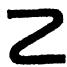
\includegraphics[keepaspectratio]{images/part003_0bad14cb.jpg}}

由命题 2 推出，有限个下半连续函数的下包络仍是下半连续的；但对无穷族下半连续函数的下包络，这一般不成立。例如，设 r 为任一有理数，\(f_{r}\) 表示在 r 处等于 0 而对一切实数 \(x \neq r\) 等于 1 的函数；诸 \(f_{r}\) 的下包络是函数 g，它对每个有理数等于 0，对每个无理数等于 1（``Dirichlet 函数''），而这个函数在无理点处不下半连续。

推论. 空间 X 上一族连续实值函数的上包络在 X 上下半连续。

在第九章，§ 1，第 6 节，命题 5 中我们将证明，若 X 是可一致化的（且仅在这种情形），这个命题的逆命题为真：可一致化空间上的每个下半连续函数是一族连续函数的上包络。

命题 3. 实值函数 \(f\) （定义在拓扑空间 \(\mathbf{X}\) 上）在一点 \(a \in \mathbf{X}\) 处下半连续，当且仅当 \(\liminf_{x \to a} f(x) = f(a)\) {[}或等价地，当且仅当 \(\liminf_{x \to a} f(x) \geqslant f(a)\) {]}。

该条件是必要的。因为对任意给定的 \(h < f(a)\) ，存在一个邻域 \(V\) （在 \(a\) 处），使得 \(h < f(x)\) 对一切 \(x \in V\) 成立；因此

\[
h \leqslant \inf _ {x \in \mathbf {V}} f (x) \leqslant \liminf _ {x \rightarrow a} f (x)
\]

（§ 5，第 6 节，公式 (12)），于是 \(f(a) \leqslant \liminf_{x \to a} f(x)\) 。该条件是充分的；因为若它成立，则对每个 \(h < f(a)\) 存在一个邻域 \(V\) （在 \(a\) 处），使得 \(h \leqslant \inf_{x \in V} f(x)\) ，从而 \(f\) 在 \(a\) 处下半连续。

命题 4. 设 \(f\) 是定义在子集 \(A\) （在拓扑空间 \(X\) 中稠密）上的任意实值函数。若对每个 \(x \in X\) 令 \(g(x) = \liminf_{y \to x, y \in A} f(y)\) ，则 \(g\) 在 \(X\) 上下半连续。

因为对任意给定的 \(h < g(x)\) ，存在一个开邻域 \(\mathbf{V}\) （在 \(x\) 处），使得对一切 \(z \in \mathbf{V} \cap \mathbf{A}\) 有 \(h < f(z)\) ；而 \(\mathbf{V}\) 是它的每个点 \(y\) 的邻域；于是 \(\liminf_{z \to y, z \in \mathbf{A}} f(z) = g(y) \geqslant h\) 对一切 \(y \in \mathbf{V}\) 成立，由此即得结果。

函数 g 称为 f 的下半连续正则化。~我们类似地定义 f 的上半连续正则化。

我们也可以把 \(g\) 定义为诸下半连续函数 \(\varphi\) （定义在 \(\mathbf{X}\) 上，且满足 \(\varphi(x) \leqslant f(x)\) 对一切 \(x \in \mathbf{A}\) 成立）中最大的一个。若 \(f\) 在 \(\mathbf{A}\) 上下半连续，则由命题 3，\(g\) 是 \(f\) 到 \(\mathbf{X}\) 的一个延拓。

\section{实数的无穷和与无穷乘积}

由于 \(\mathbf{R}\) 的每一点都有可数的基本邻域系（§ 1，第 4 节，命题 3 的推论），由此推出，有限实数的族 \((x_{t})\) 在 \(\mathbf{R}\) 中可和只当指标 \(t\) （满足 \(x_{t} \neq 0\) ）组成的集合是可数的（第三章，§ 5，第 2 节，命题 1 的推论）。于是 \(\mathbf{R}\) 中可和族的研究本质上归结为可和序列的研究。然而，以后我们不得不考虑不可数的有限实数族 \((x_{t})\) ，其各项是参数 \(t\) 的函数；可能发生这样的情形：对一切 t 该族可和，但由指标 \(\iota\) （满足 \(x_{t} \neq 0\) ）组成的（可数）集合依赖于 t。由于这个原因，下面我们对指标集的势不作任何假设。

\subsection{R 中可和的正有限数族}

定理 1. 族 \((x_{t})\) （由有限实数 \(\geqslant 0\) 组成）在 \(\mathbf{R}\) 中可和当且仅当该族的有限部分和组成的集合在 \(\mathbf{R}\) 中上有界。此时，该集合的上确界就是族 \((x_{t})\) 的和。

对指标集 I 的每个有限子集 H，令 \(s_{H} = \sum_{i \in H} x_{i}\) ；由于诸 \(x_{i}\) \(\geqslant 0\) ，关系 \(H \subset H'\) 蕴含 \(s_{H} \leqslant s_{H'}\) 。换句话说，映射 \(H \to s_{H}\) 是 I 的有限子集组成的有向集 \(\mathfrak{F}(I)\) 上的递增函数；因此（§ 5，第 2 节，定理 2 的推论）它有有限极限当且仅当它上有界。

注. 设 \((\mathrm{H}_{\lambda})\) 是 I 的有限子集的一个族，使得对 I 的每个有限子集 H，存在指标 \(\lambda\) 满足 \(H \subset H_{\lambda}\) ；则 \((x_{t})\) 可和当且仅当诸 \(s_{H_{1}}\) 组成的族在 R 中上有界。特别地，设 \((x_{n})\) 是有限实数 \(\geqslant 0\) 的序列，且对每个整数 n 令 \(s_{n} = \sum_{p=0}^{n} x_{p}\) ；则序列 \((x_{n})\) 在 R 中可和当且仅当对一个严格递增整数序列 \((n_{k})\) ，部分序列 \((s_{n_{k}})\) 在 R 中上有界。

例. 1) 对每个数 \(q\) （满足 \(0 \leqslant q < 1\) ），序列 \((q^n)\) （'公比为 \(q''\) 的等比数列'）在 \(\mathbf{R}\) 中可和，因为 \(s_n = \frac{1 - q^{n+1}}{1 - q} \leqslant \frac{1}{1 - q}\) ；该序列的和为 \(\lim_{n \to \infty} s_n = \frac{1}{1 - q}\) 。

\begin{enumerate}
\def\labelenumi{\arabic{enumi})}
\setcounter{enumi}{1}
\tightlist
\item
  设 \(a\) 与 \(b\) 是两个数，满足 \(0 \leqslant a < 1\) 与 \(0 \leqslant b < 1\) ；则族 \((a^{m}b^{n})_{(m,n) \in \mathbb{N} \times \mathbb{N}}\) 在 \(\mathbb{R}\) 中可和。因为 \(\mathbf{N} \times \mathbf{N}\) 的每个有限子集都含于形如 \([0, p] \times [0, p]\) 的子集，且我们有
\end{enumerate}

\[
\sum_ {m = 0} ^ {p} \sum_ {n = 0} ^ {p} a ^ {m} b ^ {n} = \left(\sum_ {m = 0} ^ {p} a ^ {m}\right) \left(\sum_ {n = 0} ^ {p} b ^ {n}\right) = \frac {1 - a ^ {p + 1}}{1 - a}. \frac {1 - b ^ {p + 1}}{1 - b} \leqslant \frac {1}{(1 - a) (1 - b)}.
\]

\begin{enumerate}
\def\labelenumi{\arabic{enumi})}
\setcounter{enumi}{2}
\tightlist
\item
  对每个整数 \(p > 1\) ，序列 \((n^{-p})\) ( \(n > 0\) )可和，因为
\end{enumerate}

\[
s _ {2 ^ {n + 1}} - s _ {2 ^ {n}} = \sum_ {k = 1} ^ {2 ^ {n}} (2 ^ {n} + k) ^ {- p} <   2 ^ {n}. (2 ^ {n}) ^ {- p}
\]

从而把这些不等式相加，得

\[
s _ {2 ^ {n}} <   \frac {1}{1 - 2 ^ {1 - p}}.
\]

\begin{enumerate}
\def\labelenumi{\arabic{enumi})}
\setcounter{enumi}{3}
\tightlist
\item
序列 \((1 / n)\) \((n > 0)\) 在 \(\mathbf{R}\) 中不可和，因为
\end{enumerate}

\[
s _ {2 ^ {n + 1}} - s _ {2 ^ {n}} = \sum_ {k = 1} ^ {2 ^ {n}} \frac {1}{2 ^ {n} + k} > \frac {2 ^ {n}}{2 ^ {n + 1}} = \frac {1}{2}
\]

从而把这些不等式相加，得

\[
s _ {2 ^ {n}} > n / 2
\]

故定理 1 的判别准则不满足。

\begin{enumerate}
\def\labelenumi{\arabic{enumi})}
\setcounter{enumi}{4}
\tightlist
\item
  设 \((\mathbf{I}_n)\) 是两两不相交的非空开区间的一个序列，它们都含于一个长度为有限数 \(l\) 的区间中。该族中有限个区间的长度之和 \(\leqslant l\) （§ 1，第 5 节），因此诸 \(\mathbf{I}_n\) 的长度组成的族在 \(\mathbf{R}\) 中可和，且其和 \(\leqslant l\) 。
\end{enumerate}

定理 2（比较原理）. 设 \((x_{\iota})_{\iota\in I}\) 与 \((y_{\iota})_{\iota\in I}\) 是有限实数 \(\geqslant 0\) 的两个族，满足 \(x_{\iota}\leqslant y_{\iota}\) 对一切 \(\iota\) 成立。若 \((y_{\iota})\) 在 \(\mathbb{R}\) 中可和，则 \((x_{\iota})\) 也可和，且我们有 \(\sum_{\iota}x_{\iota}\leqslant\sum_{\iota}y_{\iota}\) ；此外若存在指标 \(\chi\) 使 \(x_{\chi}<y_{\chi}\) ，则 \(\sum_{\iota}x_{\iota}<\sum_{\iota}y_{\iota}\) 。

假设蕴含

\[
\sum_ {\iota \in \mathbf {H}} x _ {\iota} \leqslant \sum_ {\iota \in \mathbf {H}} y _ {\iota},
\]

对 I 的每个有限子集 H 成立，定理的第一部分由此得证；关于和的不等式则由不等式延拓原理（§ 5，第 2 节，定理 1）得出。若 \(x_{\chi} < y_{\chi}\) ，则

\[
\sum_ {\iota} x _ {\iota} = x _ {\chi} + \sum_ {\iota \neq \chi} x _ {\iota} <   y _ {\chi} + \sum_ {i \neq x} y _ {\iota} = \sum_ {\iota} y _ {\iota}.
\]

这个定理提供了判断序列 \((x_{n})\) （由实数 \(\geqslant0\) 组成）在 R 中是否可和的最常用判别准则：我们设法把给定的序列与一个较简单的序列 \((y_{n})\) 相比较，后者的可和性我们已经知道。如果存在有限数 a \textgreater{} 0 ，使得从某个点起对一切 n 有 \(x_{n} \leqslant ay_{n}\) ，且 \((y_{n})\) 可和，则 \((x_{n})\) 可和；反之，如果存在有限数 b \textgreater{} 0 ，使得从某个点起对一切 n 有 \(x_{n} \geqslant by_{n}\) ，且 \((y_{n})\) 在 R 中不可和，则 \((x_{n})\) 在 R 中不可和。我们将在后续分册中看到，在最常出现的情形如何得到这样的比较序列。

例. 1) 设 \(a\) 是有限实数 \(>0\) ，考虑序列 \(\left(\frac{a^n}{n!}\right)\) ；设 \(n_0\) 是使 \(a < n_0\) 的最小整数。则

对每个 \(n \geqslant n_0\) 我们有

\[
\frac {a ^ {n}}{n !} \leqslant \frac {a ^ {n _ {0}}}{n _ {0} !} \cdot \left(\frac {a}{n _ {0}}\right) ^ {n - n _ {0}};
\]

由于 \(q = \frac{a}{n_0} < 1\) ，序列 \((q^{n - n_0})\) 可和，因此序列 \(\left(\frac{a^n}{n!}\right)\) 也可和。

\begin{enumerate}
\def\labelenumi{\arabic{enumi})}
\setcounter{enumi}{1}
\tightlist
\item
  设 \((a_{n})\) 是正数的一个可和序列。由于
\end{enumerate}

\[
\lim _ {n \rightarrow \infty} a _ {n} = 0,
\]

存在整数 \(n_0\) ，使得 \(a_n \leqslant 1\) 只要 \(n \geqslant n_0\) 。于是对每个 \(n \geqslant n_0\) 有 \(a_n^2 \leqslant a_n\) ，因此序列 \((a_n^2)\) 在 \(\mathbb{R}\) 中可和。序列 \((a_n^p)\) 对每个整数 \(p > 1\) 也可和。

\begin{enumerate}
\def\labelenumi{\arabic{enumi})}
\setcounter{enumi}{2}
\tightlist
\item
  设 \(a\) 与 \(b\) 是两个数 \(< 1\) ；则
\end{enumerate}

\[
\frac {1}{a ^ {m} + b ^ {n}} \leqslant \frac {1}{2 (\sqrt {a}) ^ {m} (\sqrt {b}) ^ {n}}
\]

因而族 \(\left(\frac{1}{a^m + b^n}\right)\) 在 \(\mathbf{R}\) 中可和。

推论. 设 \((x_{i})_{i\in I}\) 是 R 中有限数 \(\geqslant 0\) 的可和族。若 H 是 I 的任一子集，我们有

\[
\sum_ {i \in \mathbf {H}} x _ {i} \leqslant \sum_ {i \in \mathbf {I}} x _ {i},
\]

且等号仅当 \(x_{i} = 0\) 对一切 \(i \in \mathbb{C}\mathbb{H}\) 成立时才成立。

\subsection{R 中任意符号有限数的可和族}

定理 3. 设 \((x_{t})_{t\in I}\) 是有限实数的一个族；则下述命题等价：

\begin{enumerate}
\def\labelenumi{\alph{enumi})}
\item
  族 \((x_{i})\) 在 \(\mathbf{R}\) 中可和。
\item
  族 \((|x_{i}|)\) 在 \(\mathbf{R}\) 中可和。
\item
  族 \((x_{t})\) 的有限部分和组成的集合在 R 中有界。
\end{enumerate}

设 \(I_1\) 是所有 \(i \in I\) （满足 \(x_i \geq 0\) ）组成的集合，\(I_2\) 是所有 \(i \in I\) （满足 \(x_i < 0\) ）组成的集合。族 \((x_i)_{i \in I}\) {[}相应地，\((|x_i|)_{i \in I}\) {]}可和当且仅当族 \((x_i)_{i \in I_1}\) 与 \((x_i)_{i \in I_2}\) {[}相应地，\((|x_i|)_{i \in I_3}\) 与 \((|x_i|)_{i \in I_4}\) {]}中的每一个都可和（第三章，§ 5，第 3 节，命题 2 与命题 3）。而说 \((x_i)_{i \in I_1}\) 可和、或说 \((|x_i|)_{i \in I_2}\) 可和、或说族 \((x_{i})_{i\in I_1}\) 的有限部分和组成的集合有界（第 1 节，定理 1），这是一回事；把 \(I_1\) 换成 \(I_2\) ，同样的结论也成立。定理随即得出。

定理 3 表明，有限实数族在 R 中的可和性只依赖于其绝对值族的可和性。

我们回忆（第三章，§ 5，第 5 节，命题 6）：若 \((x_{t})\) 与 \((y_{t})\) 是有限实数的两个可和族，则族 \((x_{t} + y_{t})\) 可和，且 \(\sum_{i}(x_{t} + y_{t}) = \sum_{i}x_{t} + \sum_{i}y_{t}\) 。此外，若 \((x_{t})\) 是有限实数的可和族而 \(a\) 是任意有限实数，则族 \((ax_{t})\) 在 \(\mathbf{R}\) 中可和，且我们有 \(\sum_{i}ax_{t} = a\) . \(\sum_{i}x_{t}\) 。

\subsection{两个无穷和的乘积}

命题 1. 若有限实数的族 \((x_{\lambda})_{\lambda \in L}\) 与 \((y_{\mu})_{\mu \in M}\) 在 \(\mathbf{R}\) 中可和，则族 \((x_{\lambda}y_{\mu})_{(\lambda ,\mu)\in L\times M}\) 也可和，且我们有

\[
\sum_ {(\lambda , \mu) \in \mathbf {L} \times \mathbf {M}} x _ {\lambda} y _ {\mu} = (\sum_ {\lambda \in \mathbf {L}} x _ {\lambda}) (\sum_ {\mu \in \mathbf {M}} y _ {\mu}).\tag{1}
\]

\(\mathbf{L} \times \mathbf{M}\) 的每个有限子集都含于形如 \(\mathbf{H} \times \mathbf{K}\) 的有限子集，其中 \(\mathbf{H}\) 是 \(\mathbf{L}\) 的有限子集，\(\mathbf{K}\) 是 \(\mathbf{M}\) 的有限子集。根据假设，存在数 \(a > 0\) ，使得 \(\sum_{\lambda \in \mathbf{H}} |x_{\lambda}| \leqslant a\) 与 \(\sum_{\mu \in \mathbf{K}} |y_{\mu}| \leqslant a\) 对 \(\mathbf{H}\) 与 \(\mathbf{K}\) （\(\mathbf{L}\) 与 \(\mathbf{M}\) 的所有有限子集）分别成立；因此

\[
\sum_ {(\lambda , \mu) \in \mathbf {H} \times \mathbf {K}} | x _ {\lambda} y _ {\mu} | = (\sum_ {\lambda \in \mathbf {H}} | x _ {\lambda} |) (\sum_ {\mu \in \mathbf {K}} | y _ {\mu} |) \leqslant a ^ {2},
\]

而由定理 1 与定理 3，这表明族 \((x_{\lambda}y_{\mu})\) 在 \(\mathbf{R}\) 中可和。由结合律我们可以写{[}第三章，§ 5，第 3 节，公式 (2){]}

\[
\sum_ {(\lambda , \mu) \in \mathbf {L} \times \mathbf {M}} x _ {\lambda} y _ {\mu} = \sum_ {\lambda \in \mathbf {L}} (\sum_ {\mu \in \mathbf {M}} x _ {\lambda} y _ {\mu}) = \sum_ {\lambda \in \mathbf {L}} x _ {\lambda} (\sum_ {\mu \in \mathbf {M}} y _ {\mu}) = (\sum_ {\lambda \in \mathbf {L}} x _ {\lambda}) (\sum_ {\mu \in \mathbf {M}} y _ {\mu});
\]

由此即得结论。

\subsection{R* 中可乘的族}

在有限非零实数的乘法群 \(\mathbb{R}^*\) 中，族 \((x_{t})_{i\in I}\) 只当 \(\lim x_{t} = 1\) （关于 I 的有限子集的余集组成的滤子）时才可能可乘（第三章，§ 5，第 2 节，命题 1）。特别地，指标 \(i\) （使 \(x_{t} < 0\) ）只能有有限多个。因此我们可以限于只考虑各项都严格为正的族 \(x_{t}\) ；这时令 \(x_{i} = i + u_{i}\) 是方便的，其中诸 \(u_{i}\) 满足不等式 \(-i < u_{i} < +\infty\) （对一切 \(i\) ）。由于 \(\mathbf{R}^*\) 的每一点都有可数的基本邻域系，指标 \(i\) （使 \(u_{i} \neq 0\) ）组成的集合是可数的，只要族 \((i + u_{i})\) 在 \(\mathbf{R}^*\) 中可乘。

定理 4. 族 \((1 + u_{t})\) 在 \(\mathbb{R}^*\) 中可乘当且仅当族 \((u_{t})\) 在 \(\mathbb{R}\) 中可和。

引理. (i) 若 \((a_{i})_{1\leqslant i\leqslant p}\) 是数 \(>0\) 的一个有限序列，则

\[
\prod_ {i = 1} ^ {p} \left(1 + a _ {i}\right) \geqslant 1 + \sum_ {i = 1} ^ {p} a _ {i}.\tag{2}
\]

\begin{enumerate}
\def\labelenumi{(\roman{enumi})}
\setcounter{enumi}{1}
\tightlist
\item
  若又有 \(a_i < 1\) 对每个 \(i\) 成立，则
\end{enumerate}

\[
\prod_ {i = 1} ^ {p} \left(\mathrm{I} - a _ {i}\right) \geqslant \mathrm{I} - \sum_ {i = 1} ^ {p} a _ {i}.\tag{3}
\]

这些不等式当 \(p = 1\) 时是显然的，并可对 \(p\) 用归纳法证明。若

\[
\prod_ {i = 1} ^ {p - 1} \left(\mathrm{I} + a _ {i}\right) \geqslant \mathrm{I} + \sum_ {i = 1} ^ {p - 1} a _ {i},
\]

则我们有

\[
\prod_ {i = 1} ^ {p} \left(\mathrm{I} + a _ {i}\right) \geqslant \left(\mathrm{I} + a _ {p}\right) \left(\mathrm{I} + \sum_ {i = 1} ^ {p - 1} a _ {i}\right) = \mathrm{I} + \sum_ {i = 1} ^ {p} a _ {i} + a _ {p}. \sum_ {i = 1} ^ {p - 1} a _ {i} \geqslant \mathrm{I} + \sum_ {i = 1} ^ {p} a _ {i}.
\]

同样，若

\[
\prod_ {i = 1} ^ {p - 1} \left(\mathrm{I} - a _ {i}\right) \geqslant \mathrm{I} - \sum_ {i = 1} ^ {p - 1} a _ {i},
\]

则我们有

\[
\prod_ {i = 1} ^ {p} \left(\mathrm{I} - a _ {i}\right) \geqslant \left(\mathrm{I} - a _ {p}\right) \left(\mathrm{I} - \sum_ {i = 1} ^ {p - 1} a _ {i}\right) = \mathrm{I} - \sum_ {i = 1} ^ {p} a _ {i} + a _ {p}. \sum_ {i = 1} ^ {p - 1} a _ {i} \geqslant \mathrm{I} - \sum_ {i = 1} ^ {p} a _ {i}.
\]

证明了引理之后，我们注意，若族 \((\mathbf{I} + u_{t})\) 可乘，则族 \((\mathbf{I} + u_{t}^{+})\) 与 \((\mathbf{I} - u_{t}^{-})\) 也可乘，因为 \(\mathbf{R}^*\) 是完备群（第三章，§ 5，第 3 节，命题 2）；反之，若族 \((\mathbf{I} + u_{t}^{+})\) 与 \((\mathbf{I} - u_{t}^{-})\) 可乘，则 \((\mathbf{I} + u_{t})\) 也可乘（第三章，§ 5，第 3 节，命题 3）。因此我们只需考虑两种情形：一切 \(u_{t}\) 都 \(\geqslant 0\) ，或它们都 \(\leqslant 0\) 。

首先设 \(u_{t} \geqslant 0\) 对一切 \(t\) 成立。若族 \((1 + u_{t})\) 可乘，则对每个 \(\varepsilon > 0\) ，存在一个有限子集 \(J\) （属于指标集 \(I\) ），使得对每个有限子集 \(H\) （含于 \(I\) 且与 \(J\) 不相交），有 \(\mathbf{I} \leqslant \prod_{i \in \mathbf{H}} (\mathbf{I} + u_i) \leqslant \mathbf{I} + \varepsilon\) ；由 (2) 推出 \(\sum_{i \in \mathbf{H}} u_i \leqslant \varepsilon\) ，这表明由 Cauchy 判别准则（第三章，§ 5，第 2 节，定理 I），\((u_i)\) 在 \(\mathbf{R}\) 中可和。

反之，设 \((u_{t})\) 在 \(\mathbf{R}\) 中可和。对每个 \(\varepsilon\) （满足 \(0 < \varepsilon < 1\) ），存在一个有限子集 \(J\) （\(I\) 的），使得对每个有限子集 \(H\) （含于 \(I\) 且与 \(J\) 不相交），有 \(0 \leqslant \sum_{t \in H} u_{t} \leqslant \varepsilon\) 。由 (3)，我们因此有 \(\prod_{t \in H} (I - u_{t}) \geqslant I - \varepsilon\) ；但由于 \(I + u \leqslant \frac{I}{I - u}\) 对每个数 \(u\) （满足 \(0 \leqslant u < 1\) ）成立，由此推出

\[
\mathrm{I} \leqslant \prod_ {i \in \mathrm{H}} (\mathrm{I} + u _ {i}) \leqslant \frac {\mathrm{I}}{\mathrm{I} - \varepsilon},
\]

而这表明 \((\mathbf{I} + u_{t})\) 可乘（Cauchy 判别准则）。

当一切 \(u_{i}\) 都 \(\leqslant 0\) 时证明类似。为证明 \((u_{i})\) 可和当 \((1 + u_{i})\) 可乘，用公式 (2) 及不等式 \(1 - u \leqslant \frac{1}{1 + u}\) ( \(0 \leqslant u < 1\) )；为证明 \((1 + u_{i})\) 可乘当 \((u_{i})\) 可和，用公式 (3)。

在第五章（§ 4）中，群 \(\mathbf{R}^*\) 的拓扑研究将使我们能借助对数函数给出族在 \(\mathbf{R}^*\) 中可乘的另一个判别准则；在后续分册中我们将利用对数的微分性质证明这个判别准则与上面那个等价。

\subsection{\texorpdfstring{\(\overline{\mathbf{R}}\) 中的可和族与可乘族}{SUMMABLE FAMILIES AND MULTIPLIABLE FAMILIES IN \textbackslash overline\{\textbackslash mathbf\{R\}\}}}

在区间 \([0, +\infty]\) （\(\overline{\mathbf{R}}\) 中的）上，加法是一个结合的、交换的合成法则（§ 4，第 3 节）；因此在该区间中数的可和族的概念已有定义（第三章，§ 5，第 1 节，注 3）。

命题 2. 族 \((x_{\mathfrak{t}})\) （由实数 \(\geqslant 0\) 组成）的每一个在 \(\overline{\mathbf{R}}\) 中可和。因为映射 \(\mathbf{H} \to s_{\mathbf{H}}\) （由有向集 \(\mathfrak{F}(\mathbf{I})\) 到 \(\overline{\mathbf{R}}\) 中）是递增的；故（§ 5，第 2 节，定理 2）有极限。

同样的推理表明，实数 \(\leqslant 0\) 的每个族在 \(\overline{\mathbf{R}}\) 中可和。

类似地，乘法在区间 \([0, 1]\) 与 \([1, +\infty]\) （\(\overline{R}\) 中的）的每一个上都是一个结合的、交换的合成法则，因此可乘族的概念在每个这样的区间上都有定义。

命题 3. 每个族 \((1 + u_{t})\) {[}相应地，\((1 - u_{t})]\) ——由数 \(\geqslant 1\) （相应地，\(\geqslant 0\) 且 \(\leqslant 1\) ）组成——在 \(\overline{\mathbf{R}}\) 中可乘。

与命题 2 的证明相同。

推论. 积 \(\prod_{i} (1 + u_i) [\text{resp. } \prod_{i} (1 - u_i))\) （由数 \(\geqslant 1\) （相应地，\(>0\) 且 \(\leqslant 1\) ）组成）等于 \(+\infty\) （相应地，0）当且仅当 \(\sum_{i} u_i = +\infty\) 。因为若 \(\sum_{i} u_i\) 有限，则 \(\prod_{i} (1 + u_i)\) 与 \(\prod_{i} (1 - u_i)\) 属于 \(\mathbf{R}^*\) ，反之亦然（第 4 节，定理 4）。

注. 结合性定理（第三章，§ 5，第 3 节，定理 2）当把 G 换成 \(\overline{\mathbf{R}}\) 并假设诸 \(x_{i}\) \(\geqslant 0\) 时仍然成立。若 \(\sum_{i \in I} x_{i}\) 有限，这是显然的。反之设 \(\sum_{i \in I} x_{i} = +\infty\) 。则对每个有限的 \(a > 0\) ，存在 I 的有限子集 H 使得 \(\sum_{i \in H} x_{i} \geqslant a\) 。设 K 是 L 的有限子集且 \(H \subset \bigcup_{\lambda \in K} I_{\lambda}\) ；那么由于 \(s_{\lambda} \geqslant \sum_{i \in I_{\lambda} \cap H} x_{i}\) 对一切 \(\lambda \in K\) ，我们有

\[
\sum_ {\lambda \in \mathbf {K}} s _ {\lambda} \geqslant \sum_ {i \in \mathbf {H}} x _ {i} \geqslant a,
\]

这表明 \(\sum_{\lambda \in L} s_{\lambda} = +\infty\) 。我们把对 \([0, 1]\) 或 \([1, +\infty]\) 中的数的可乘族表述类似命题的任务留给读者。

\subsection{实数的无穷级数与无穷乘积}

有限实数的级数，若它在 R 中收敛，就简称为收敛的。

定义 1. 有限实数的级数称为绝对收敛的，如果其各项的绝对值组成的级数收敛。

命题 4. 有限实数的级数交换收敛当且仅当它绝对收敛。

这由第三章，§ 5，第 7 节，命题 9 以及第 2 节的定理 3 得出。

换句话说，若 \((u_{n})\) 是有限实数的序列，则说通项为 \(u_{n}\) 的级数交换收敛、或说它绝对收敛、或说序列 \((u_{n})\)

在 \(\mathbf{R}\) 中可和，这是一回事。于是第三章 § 5 中证明的可和族的一切性质都可应用于绝对收敛级数。特别地，若通项为 \(u_{n}\) 的级数绝对收敛，则和 \(\sum_{n\in\mathbf{H}} u_{n}\) 对子集 \(\mathbf{H}\) （\(\mathbf{N}\) 的所有子集）存在；又若 \((\mathbf{H}_{p})\) 是 \(\mathbf{N}\) 的一个分拆，我们有

\[
\sum_ {n = 0} ^ {\infty} u _ {n} = \sum_ {p} \left(\sum_ {n \in \mathrm{H} _ {p}} u _ {n}\right)
\]

（绝对收敛级数的结合性）。

正如我们已在第三章 § 5 中指出的，实数级数可以收敛而不交换收敛，即不绝对收敛。

例. 交错级数. 由有限实数的序列 \((u_n)\) 定义的级数称为交错的，如果 \(u_n = (-1)^n v_n\) ，其中 \(v_n \geqslant 0\) 对一切 \(n\) 成立。我们来证明，这类级数收敛的一个充分条件是序列 \((v_n)\) 递减且以 \(0\) 为其极限。因为若 \(s_n\) 表示

\[
\sum_ {p = 0} ^ {n} u _ {p},
\]

\((v_{n})\) 递减这一假设蕴含

\[
s _ {2 n + 1} \leqslant s _ {2 n + 3} \leqslant s _ {2 n + 2} \leqslant s _ {2 n}
\]

对一切 \(n \geqslant 0\) 。序列 \((s_{2n})\) {[}相应地，\((s_{2n+1})\) {]}递减且下有界（相应地，递增且上有界），因此有有限极限 a（相应地，b），且 \(b \leqslant a\) ；由于

\[
a - b = \lim _ {n \rightarrow \infty} (s _ {2 n} - s _ {2 n + 1}) = \lim _ {n \rightarrow \infty} v _ {2 n + 1} = 0,
\]

断言得证。

例如若取 \(v_{n}=1/n\) ，上述条件满足，因此通项为 \((-1)^{n}/n\) 的级数（``交错调和级数''）收敛。我们在第 1 节已看到，通项为 1/n 的级数（``调和级数''）不收敛，从而交错调和级数不绝对收敛。

我们回忆（第三章，§ 5，第 6 节，命题 7）：若 \((u_n)\) 与 \((v_n)\) 是有限实数的两个收敛级数，则级数 \((u_n + v_n)\) 收敛，且

\[
\sum_ {n = 0} ^ {\infty} \left(u _ {n} + v _ {n}\right) = \sum_ {n = 0} ^ {\infty} u _ {n} + \sum_ {n = 0} ^ {\infty} v _ {n};
\]

又，若级数 \((u_{n})\) 收敛，则级数 \((au_{n})\) 对一切有限实数 \(a\) 收敛，且 \(\sum_{n=0}^{\infty} au_{n} = a\) . \(\sum_{n=0}^{\infty} u_{n}\) 。

最后，若级数 \((u_n)\) 与 \((v_n)\) 收敛，且 \(u_n \leqslant v_n\) 对一切 \(n\) ，则由不等式延拓原理（§ 5，第 2 节，定理 1），\(\sum_{n=0}^{\infty} u_n \leqslant \sum_{n=0}^{\infty} v_n\) 。

应当注意，若设级数 \((v_{n})\) 收敛但不绝对收敛，且对每个 n 有 \(|u_{n}| \leqslant |v_{n}|\) ，我们决不能推断级数 \((u_{n})\) 收敛，取 \(u_{n} = |v_{n}|\) 即见。

有限非零实数的无穷乘积，若它在 \(\mathbf{R}^*\) 中收敛，就简称为收敛的；此时它的值是有限的非零实数。

定义 2. 通项因子为 \(1 + u_{n}\) 的无穷乘积称为绝对收敛的，如果通项因子为 \(1 + |u_{n}|\) 的乘积收敛。

命题 5. 有限实数的无穷乘积交换收敛当且仅当它绝对收敛。

这由第三章，§ 5，第 7 节，命题 9 以及上面的定理 4 得出。

此外，通项因子为 \(1 + u_{n}\) 的乘积绝对收敛当且仅当通项为 \(u_{n}\) 的级数绝对收敛。

非零实数的乘积可以收敛而不交换收敛，即不绝对收敛。

例. 若取 \(u_{2n-1} = -\frac{1}{n}\) 与 \(u_{2n} = \frac{1}{n}\) （对 \(n \geqslant 2\) ），则乘积 \((1 + u_n)\) 不绝对收敛，因为级数 \((u_n)\) 不绝对收敛；但由于

\[
\begin{array}{l} \prod_ {p = 3} ^ {n} (1 + u _ {p}) = \prod_ {p = 2} ^ {n} \left(1 - \frac {1}{p ^ {2}}\right), \\ \text { and } \quad \prod_ {p = 3} ^ {2 n + 1} (1 + u _ {p}) = \left(1 - \frac {1}{n + 1}\right) \prod_ {p = 2} ^ {n} \left(1 - \frac {1}{p ^ {2}}\right), \end{array}
\]

由定理 4 推出该乘积收敛，且其值为

\[
\prod_ {n = 2} ^ {\infty} \left(1 - \frac {1}{n ^ {2}}\right).
\]

\pandocbounded{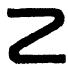
\includegraphics[keepaspectratio]{images/part003_4cdcc444.jpg}}

此外应当指出，通项为 \(u_{n}\) 的级数的收敛性对于通项因子为 \(1 + u_{n}\) 的乘积的收敛性既不必要也不充分（见习题 21 与 22）。

\section{实数的通常展开；R 的势}

\subsection{实数的近似}

定义 1. 给定一个数 \(\varepsilon > 0\) ，实数 \(r\) 称为精确到 \(\varepsilon\) 的实数 \(x\) 的近似，如果 \(|x - r| \leqslant \varepsilon\) ；\(r\) 称为不足近似，如果 \(r \leqslant x\) ；称为过剩近似，如果 \(r \geqslant x\) 。

设 A 是 R 的一个稠密子集。对每个 \(x \in R\) 与每个 \(\varepsilon > 0\) ，存在 x 的属于 A 的精确到 \(\varepsilon\) 的不足（相应地，过剩）近似，因为区间 \(]x - \varepsilon, x[\) （相应地，\(]x, x + \varepsilon[\) ）至少含有 A 的一个点。现在若考虑一个给定的严格递减序列 ( \(\varepsilon_{n}\) ) （由数 \textgreater{} 0 组成，趋于 0），而 \(r_{n}\) 是 x 的精确到 \(\varepsilon_{n}\) 的近似，则序列 ( \(r_{n}\) ) 当 n 趋于无穷时以 x 为极限。

在 A 是加法群 R 的子群且限制 \(\varepsilon_{n}\) 属于 A 的情形，我们对每个 \(x \in R\) 都能按典型方式定义一个由 x 的属于 A 的不足近似组成的序列 \((r_{n})\) 。

因为由 Archimedes 公理（§ 2，第 1 节，定理 1），整数 \(p\) （满足 \(p\varepsilon_n \leqslant x\) ）组成的集合有一个最大元 \(p_n\) ；换言之，存在唯一的整数 \(p_n\) 使得

\[
p _ {n} \varepsilon_ {n} \leqslant x <   (p _ {n} + 1) \varepsilon_ {n}.\tag{1}
\]

由于 \(|x - p_n\varepsilon_n| \leqslant \varepsilon_n\) ，由此推出 \(p_n\varepsilon_n\) 是 \(x\) 的精确到 \(\varepsilon_n\) 的不足近似，且由假设属于 A；类似地，\((p_n + 1)\varepsilon_n\) 是 \(x\) 的属于 A 的精确到 \(\varepsilon_n\) 的过剩近似，而两个序列 \((p_n\varepsilon_n)\) 与 \(((p_n + 1)\varepsilon_n)\) 都以 \(x\) 为极限。

\subsection{实数关于基序列的展开}

我们将限于研究 \(\varepsilon_{n} = 1 / d_{n}\) 的情形，其中 \((d_n)\) 是整数的一个严格递增序列，满足 \(d_0 = 1\) ，且 \(d_n\) 是 \(d_{n-1}\) 的倍数（对 \(n \geqslant 1\) ）。令 \(a_n = d_n / d_{n-1}\) ( \(n \geqslant 1\) )：\(a_n\) 是一个整数 \(>1\) 。在这种情形，不足近似 \(r_n = p_n / d_n\) 组成的序列是递增的，因为 \(p_n\) 是使 \(p_n / d_n \leqslant x\) 成立的最大整数；

但我们有

\[
\frac {p _ {n - 1}}{d _ {n - 1}} = \frac {p _ {n - 1} a _ {n}}{d _ {n}} \leqslant x <   \frac {p _ {n - 1} + 1}{d _ {n - 1}} = \frac {p _ {n - 1} a _ {n} + a _ {n}}{d _ {n}}
\]

于是 \(a_{n}p_{n - 1}\leqslant p_{n} <   a_{n}p_{n - 1} + a_{n},\) ，因此 \(r_{n - 1}\leqslant r_n\leqslant x.\) 令

\[
p _ {n} = a _ {n} p _ {n - 1} + u _ {n};\tag{2}
\]

则 \(0 \leqslant u_n < a_n\) ，它等价于 \(0 \leqslant u_n \leqslant a_n - 1\) ，因为 \(u_n\) 是整数。由此

\[
r _ {n} = r _ {n - 1} + \frac {u _ {n}}{d _ {n}} = p _ {0} + \sum_ {k = 1} ^ {n} \frac {u _ {k}}{d _ {k}},\tag{3}
\]

并且，由于 \(x = \lim_{n\to \infty}r_n,\)

\[
x = p _ {0} + \sum_ {n = 1} ^ {\infty} \frac {u _ {n}}{d _ {n}}.\tag{4}
\]

(4) 右端的级数，其和为 \(x\) ，称为 \(x\) 关于基序列 \((d_n)\) 的展开。所有系数 \(u_n\) 都 \(\geqslant 0\) ；\(p_0\) 依定义是最大整数 \(p\) （满足 \(p \leqslant x\) ）；它称为 \(x\) 的整数部分，常记作 {[}x{]}。

\subsection{用展开式定义实数}

反之，设给定了一个整数 \(q_0\) 与整数的序列 \((v_n)\) ( \(n \geqslant 1\) )（满足 \(0 \leqslant v_n \leqslant a_n - 1\) ）；我们问是否存在一个数 \(x\) ，其展开 (4) 满足 \(p_0 = q_0\) 且 \(u_n = v_n\) 对一切 \(n\) 。如果这样的数存在，它就是唯一的，因为它等于 \(q_0 + \sum_{n=1}^{\infty} \frac{v_n}{d_n}\) 。

对每个整数 \(m > 0\) 我们有（由比较原理）

\[
\sum_ {n = m + 1} ^ {\infty} \frac {v _ {n}}{d _ {n}} \leqslant \sum_ {n = m + 1} ^ {\infty} \frac {a _ {n} - 1}{d _ {n}} = \sum_ {n = m + 1} ^ {\infty} \left(\frac {1}{d _ {n - 1}} - \frac {1}{d _ {n}}\right) = \frac {1}{d _ {m}}
\]

而且最左端与最右端的项仅当 \(v_{n} = a_{n} - 1\) （对每个 \(n > m\) ）时才相等（§ 7，第 1 节，定理 2）。因此通项为 \(\frac{v_n}{d_n}\) 的级数收敛；此外，若 \(x = q_0 + \sum_{n=1}^{\infty} \frac{v_n}{d_n}\) ，我们有

\[
s _ {m} = q _ {0} + \sum_ {n = 1} ^ {m} \frac {v _ {n}}{d _ {n}} \leqslant x \leqslant s _ {m} + \frac {1}{d _ {m}}
\]

且 \(x = s_m + \frac{1}{d_m}\) 仅当 \(v_n = a_n - 1\) （对每个 \(n > m\) ）时成立。由于 \(s_m\) 是分母为 \(d_m\) 的分数，不足近似 \(r_m\) （它对 \(x\) 精确到 \(1/d_m\) ）等于 \(s_m\) 或 \(s_m + \frac{1}{d_m}\) ；且后一情形仅当 \(v_{n} = a_{n} - 1\) （对一切 \(n > m\) ）时才能发生。于是：

\begin{enumerate}
\def\labelenumi{(\roman{enumi})}
\item
  存在无穷多个 \(n\) 的值（满足 \(v_{n} < a_{n} - 1\) ）：这时级数 \(q_{0} + \sum_{n=1}^{\infty} \frac{v_{n}}{d_{n}}\) 与其和 \(x\) 的展开完全相同。
\item
  存在一个整数 \(m \geqslant 0\) 使得 \(v_{n} = a_{n} - 1\) （只要 \(n > m\) ），且 \(v_{m} < a_{m} - 1\) （若 \(m > 0\) ）；这时 \(x\) （级数 \(q_{0} + \sum_{n=1}^{\infty} \frac{v_{n}}{d_{n}}\) 的和）等于有理数
\end{enumerate}

\[
q _ {0} + \sum_ {n = 1} ^ {m} \frac {v _ {n}}{d _ {n}} + \frac {1}{d _ {m}}\tag{5}
\]

它是 \(k/d_{m}\) 型的（k 为整数）；x 的展开与级数 (5) 完全相同，其中所有指标 \textgreater{} m 的项都是零；这样的展开称为是有限的，或说是终止的。级数

\[
q _ {0} + \sum_ {n = 1} ^ {\infty} \frac {v _ {n}}{d _ {n}} = q _ {0} + \sum_ {n = 1} ^ {m} \frac {v _ {n}}{d _ {n}} + \sum_ {n = m + 1} ^ {\infty} \frac {a _ {n} - 1}{d _ {n}}\tag{6}
\]

称为数 x 的非正常展开。

反之，设 x 是一个有理数，它对 n 的某个值可以写成分母为 \(d_{n}\) 的分数。~设 m 是使 x 为 \(k/d_{m}\) 型（k 为整数）的最小整数；我们有 \(r_{n}<x\) （对 n\textless m），且 \(r_{m}=x\) ，因此 x 的展开具有形式 (5)，且 x 有一个由 (6) 给出的非正常展开；此外这个非正常展开是唯一的。

一个有理数，写成既约形式 \(p / q\) ，等于分母为 \(d_n\) 的分数当且仅当 \(q\) 整除 \(d_n\) （数 \(m\) 因而是这样的最小整数 \(n\) ：\(q\) 整除 \(d_n\) ）。可能发生这样的情形：每个有理数都具有这一性质（对适当选取的 \(n\) ）；当且仅当每个整数 \(> 0\) 整除某个 \(d_n\) （例如 \(d_n = n!\) ）时才是这种情形。如果诸 \(d_n\) 具有这一性质，那么一个数是有理数当且仅当它关于序列 \((d_n)\) 的展开终止。

概括起来：对每个序列 \(s\) ，其首项 \(q_{0}\) 是任意整数，且其项 \(v_{n}(n \geqslant 1)\) 满足 \(0 \leqslant v_{n} \leqslant a_{n} - 1\) ，对应着一个等于 \(q_{0} + \sum_{n=1}^{\infty} \frac{v_{n}}{d_{n}}\) 的实数；若 \(I_{n}\) 表示区间 \([0, a_{n} - 1]\) （\(N\) 中的），我们就这样定义了一个映射 \(\varphi\) （从 \(X = Z \times \prod_{n=1}^{\infty} I_{n}\) 到直线 \(R\) 上）；此外，方程 \(\varphi(s) = x\) ——其中 \(x \in R\) 已给定——当 \(x\) 不是分母为 \(d_{n}\) （对某个 \(n\) ）的分数时有一个解，否则有两个解。

\subsection{展开式的比较}

如果我们知道两个不同实数 \(x\) 与 \(y\) 的展开，就能判定是 \(x < y\) 还是 \(x > y\) 。

设 \(x = p_0 + \sum_{n=1}^{\infty} u_n / d_n\) ，\(y = q_0 + \sum_{n=1}^{\infty} v_n / d_n\) 是 \(x\) 与 \(y\) 的展开。若 \(p_0 < q_0\) 则 \(x < y\) ，因为

\[
p _ {0} \leqslant x <   p _ {0} + 1 \leqslant q _ {0} \leqslant y.
\]

更一般地，设 \(p_0 = q_0\) 且 \(u_n = v_n\) （对 \(1 \leqslant n \leqslant m\) ），但 \(u_m < v_m\) ；如果

\[
r _ {n} = p _ {0} + \sum_ {k = 1} ^ {n} u _ {k} / d _ {k}, \quad s _ {n} = q _ {0} + \sum_ {k = 1} ^ {n} v _ {k} / d _ {k},
\]

则 \(r_n = s_n\) （对 \(n < m\) ），且由于 \(u_m + 1 \leqslant v_m\) ，有 \(r_m + \frac{1}{d_m} \leqslant s_m\) ；但 \(r_m \leqslant x < r_m + \frac{1}{d_m} \leqslant s_m \leqslant y\) ，因此再次有 \(x < y\) 。换言之，\(x\) 与 \(y\) 的次序同于它们各自的展开中头两个不同项的次序。

由此推出，若 \(p_{0}=q_{0}\) 且 \(u_{n}=v_{n}\) （对 n\textless m），则每个属于以 x 与 y 为端点的闭区间的数 z 的展开的前 m 项与 x 与 y 的展开的前 m 项相同。

我们还注意，在这种情形有 \(|y - x| \leqslant \frac{1}{d_{m-1}}\) 。如果我们赋予

Z 与诸区间 \(I_{n}\) 以离散拓扑，则由此推出上面定义的映射 \(\varphi\) 在乘积空间 X 上连续。

\subsection{以 a 为底的展开}

最重要的基序列是那些 \(d_{n}=a^{n}\) 的序列，其中 a 是整数 \textgreater1；这时 a 称为相应展开的底数（或简称底）。对于数值计算，使用以 10 为底的展开，称为十进展开；以 2 为底（二进展开）与以 3 为底（三进展开）的展开也常被使用。

为了表示不足近似 \(r_n\) （对数 \(x \geqslant 0\) ，在其以 \(a\) 为底的展开中），采用下述记号：每个整数 \(u\) （满足 \(0 \leqslant u \leqslant a - 1\) ）用一个特定的记号表示；如果

\[
r _ {n} = p _ {0} + \sum_ {k = 1} ^ {n} \frac {u _ {k}}{d _ {k}},
\]

我们首先借助这些记号写出以 \(a\) 为底的整数 \(p_{0}=[x]\geqslant0\) 的表示（集合论，第三章，§ 5，第 7 节），然后放一个点（``小数点''），并写出

相继地表示数 \(u_1, u_2, \ldots, u_n\) 的记号。如果 \(S\) 是这样得到的符号，习惯上（滥用语言）写 \(x = S \ldots\) 。应当一劳永逸地理解：这样的关系式只是指示右端是 \(x\) 的精确到 \(1/a^n\) 的不足近似的一种缩写方法。

对于负数，通行习惯不同：我们用上述记号写出 \(x' = -x > 0\) 的一个近似，并在其前放置符号``-''；因此这样记的是 \(x\) 的精确到 \(1/a^n\) 的过剩近似。

这个用法对数值计算有其不便之处。在负对数的记号中，采用与正数相同的记号，而在整数部分上放一横杠，以指示它等于所写数的相反数。

\subsection{R 的势}

我们有 \(\mathbf{R} = \bigcup_{n\in \mathbf{Z}}[n,n + 1[,\) 且所有区间 \([n,n + 1[\) 都与 \([0,1[\) 等势。由于 \([0,1[\) 是无限集，由此推出 \(\mathbf{R}\) 与区间 \([0,1[\) 等势。通过考虑区间 \([0,1[\) 中数的二进展开，我们将证明这个区间与由每一项都等于 0 或 1 的序列 \((u_n)\) 组成的集合 S 等势。

首先，它与子集 \(S'\) （\(S\) 的，由序列 \((u_n)\) （满足 \(u_n = 0\) ，对无穷多个 \(n\) 的值）组成）等势。另一方面，余集 \(S''\) （\(S'\) 在 \(S\) 中的）与等于分母为 \(2^n\) 的分数的有理数的所有非正常展开组成的集合等势；这些数构成 \(Q\) 的一个子集，因此它们组成的集合是可数的，从而 \(S''\) 也是可数的。由于 \(S'\) 是无限的，它与 \(S\) 等势，由此即得结果。

现在 S 与 \(\mathfrak{P}(\mathbf{N})\) 等势；因为我们可以定义 \(\mathfrak{P}(\mathbf{N})\) 到 S 上的一个双射，把 N 的每个子集 A 映为序列 \((u_n)\) ，其中 \(u_n = 0\) 若 \(n \in A\) ，而 \(u_n = 1\) 若 \(n \in \mathbb{C}A\) 。我们这样就证明了：

定理 1（Cantor）. 实数组成的集合与一个可数无限集的一切子集组成的集合等势。

推论. 实数组成的集合的势严格大于可数集的势。

与 R 等势的集合称为具有连续统的势。由 § 4 第 1 节命题 1，每个含有多于一个点的区间都具有连续统的势。同样，R 的可数子集的余集具有连续统的势；特别地，所有无理数组成的集合具有连续统的势。

\BourbakiExercises
\BourbakiExerciseGroup

\begin{enumerate}
\def\labelenumi{\arabic{enumi})}
\tightlist
\item
  一个拓扑 \(\mathfrak{G}\) （在有序交换群 \(\mathbf{G}\) 上）称为与 \(\mathbf{G}\) 的序群结构相容，如果它与 \(\mathbf{G}\) 的群结构相容，此外集合 \(\mathbf{G}_{+}\) （由元素 \(x \geqslant 0\) （属于 \(\mathbf{G}\) ）组成）关于 \(\mathfrak{G}\) 是闭的。
\end{enumerate}

\begin{enumerate}
\def\labelenumi{\alph{enumi})}
\item
  设 \(\mathfrak{G}\) 是与 \(\mathbf{G}\) 的序群结构相容的一个 Hausdorff 拓扑，又设 \(\hat{\mathbf{G}}\) 是 \(\mathbf{G}\) 的完备化（关于 \(\mathfrak{G}\) ）。在群 \(\hat{\mathbf{G}}\) 中，闭包 \(\mathbf{P}\) （\(\mathbf{G}_{+}\) 的）是这样的：\(y - x \in \mathbf{P}\) 是一个与 \(\hat{\mathbf{G}}\) 的群结构相容的预序。
\item
  设 \(\theta\) 是一个无理数，考虑 \(\mathbf{Q}^2\) 上的这样一个序：其正元素组成的集合由 (0, 0) 与所有偶 \((x, y)\) （满足 \(y - \theta x \geqslant 0\) ）组成。关于这个序，\(\mathbf{Q}^2\) 是一个全序群，而 \(\mathbf{Q}^2\) 上由有理直线的拓扑与自身的乘积给出的拓扑与这个序群结构相容。但在 \(\hat{\mathbf{G}} = \mathbb{R}^2\) 上，关系 \(y - x \in \mathbf{P} = \overline{\mathbf{G}}_+\) 不是序。
\item
  在全序群 G 上，拓扑 \(\mathfrak{C}_{0}(\mathbf{G})\) （第一章，§ 2，习题 5）是与序群结构相容的所有拓扑中最粗的（区分两种情形，视所有 \(x > 0\) 组成的集合有还是没有最小元素而定）。G 上与 G 的群结构相容且细于 \(\mathfrak{C}_{0}(\mathbf{G})\) 的每个拓扑都与 G 的序群结构相容，且映射 \(x \to x^{+}\) 关于这样的拓扑连续。这个映射关于 \(\mathfrak{C}_{0}(\mathbf{G})\) 一致连续，但不一定关于一个群拓扑 \(\mathfrak{C}\) （严格细于 \(\mathfrak{C}_{0}(\mathbf{G})\) ）一致连续{[}见 b){]}。
\end{enumerate}

\begin{enumerate}
\def\labelenumi{\arabic{enumi})}
\setcounter{enumi}{1}
\tightlist
\item
  \begin{enumerate}
  \def\labelenumii{\alph{enumii})}
  \tightlist
  \item
    设 G 是一个格序交换群。对 G 中每个 \(x \geqslant 0\) ，令 \(\mathbf{I}(x)\) 表示 G 中的区间 \([-x, x]\) 。G 的一个非空族 \((c_{\alpha})\) （由元素 \(\geqslant 0\) 组成）使得诸区间 \(\mathbf{I}(c_{\alpha})\)
  \end{enumerate}
\end{enumerate}

构成 G 上与 G 的群结构相容的拓扑 \(\mathfrak{G}\) 在点 0 处的基本邻域系，当且仅当 \(c_{\alpha}\) 组成的集合是有向的（关于关系 \(\geqslant\) ），且对每个 \(\alpha\) 存在 \(\beta\) 使 \(2c_{\beta} \leqslant c_{\alpha}\) 。如果这些条件满足，G 到 G 中的映射 \(x \to x^{+}\) 一致连续。\(\mathfrak{G}\) 是 Hausdorff 的当且仅当 \(\inf c_{\alpha} = 0\) ；且在这种情形 \(\mathfrak{G}\) 与 G 的序群结构相容。

\begin{enumerate}
\def\labelenumi{\alph{enumi})}
\setcounter{enumi}{1}
\item
  在群 \(G = Z^{N}\) （可数无穷多个全序群 Z 的乘积）上，没有用 a) 的程序定义的非离散拓扑，但诸因子 Z 上的离散拓扑的乘积是 G 上的一个拓扑，它与 G 的序群结构相容，它是 Hausdorff 的且非离散的。
\item
  在全序群 G 上，用 a) 的程序定义的唯一 Hausdorff 拓扑是拓扑 \(\mathcal{G}_{0}(G)\) （第一章，§ 2，习题 5）。
\end{enumerate}

\begin{enumerate}
\def\labelenumi{\arabic{enumi})}
\setcounter{enumi}{2}
\tightlist
\item
  设 G 是一个格序交换群，又设 M 是 G 的上界子集组成的半群。M 的每个上有界（相应地，下有界）子集都有上确界（相应地，下确界），且 G 可以按典型方式与 M 的一个子集等同。设 G' 表示 M 的最大子群（M 的所有可对称化元素组成的集合）。
\end{enumerate}

\begin{enumerate}
\def\labelenumi{\alph{enumi})}
\tightlist
\item
  考虑一个拓扑 \(\mathcal{G}\) （在 \(\mathbf{G}\) 上，由习题 2 \(a\) ) 的程序定义）；设 \(\mathbf{V}_{\alpha}\) 是所有偶 \((z, z')\) （属于 \(\mathbf{M} \times \mathbf{M}\) ）组成的集合，使得
\end{enumerate}

\[
z - c _ {\alpha} \leqslant z ^ {\prime} \leqslant z + c _ {\alpha};
\]

证明诸 \(V_{\alpha}\) 构成 M 上一个一致结构 U 的一致邻域基本系，且 U 诱导的拓扑 \(C'\) 在 G 上诱导出 C。若 C 是 Hausdorff 的，则 U 是一个 Hausdorff 一致结构（注意 M 的元素——看作 G 的子集——这时是闭的），且这样定义的一致空间 M 是完备的。证明 M × M 到 M 中的映射 \((z, z') \to z + z'\) 一致连续。假设 C 是 Hausdorff 的，证明在 M 中 M 的任意子集的上（相应地，下）界组成的集合关于 \(C'\) 是闭的（先对 M 的一个元素的上界或下界组成的集合证明此点，把 M 的元素看作 D 的子集），且映射

\[
(z, z ^ {\prime}) \rightarrow \inf (z, z ^ {\prime})
\]

\(\mathbf{M} \times \mathbf{M}\) 到 \(\mathbf{M}\) 中的这一映射是一致连续的（同样的方法）。

\begin{enumerate}
\def\labelenumi{\alph{enumi})}
\setcounter{enumi}{1}
\item
  在本习题中从现在起设 \(\mathfrak{G}\) 是 Hausdorff 的。这时闭包 \(\overline{\mathbf{G}}\) （\(\mathbf{G}\) 在 \(\mathbf{M}\) 中的）是一个格序群，它在 \(\mathfrak{G}'\) 诱导的拓扑中是完备的。群 \(\mathbf{G}'\) 在 \(\mathbf{M}\) 中是闭的（注意它的闭包是 M 的一个子群），且 \(\mathcal{G}'\) 在 \(\mathbf{G}'\) 上诱导的拓扑与 \(\mathbf{G}'\) 的序群结构相容。为使 \(\mathbf{G}'\) 等于 \(\overline{\mathbf{G}}\) ，只需每个非空开区间 \(]a, b[\) （\(\mathbf{G}'\) 中的）含有 \(\mathbf{G}\) 的一个元素，且若 \(\mathbf{G}\) 是全序的这总是成立的。在这种情形，\(\mathbf{G}'\) 上由 \(\mathcal{G}'\) 诱导的拓扑是 \(\mathcal{C}_0(\mathbf{G}')\) 。
\item
  取 G 为有序群 \(Q^{2}\) ，即全序群 Q 与自身的乘积；这时带乘积序有 \(G' = M = R^{2}\) 。证明 G 上由习题 2 a) 的程序定义的非离散 Hausdorff 拓扑只有三个，且它们是这样得到的：取元素 \(c_{\alpha}\) 组成的集合为下列三者之一：偶 \((x, y)\) （满足 x \textgreater{} 0 与 y \textgreater{} 0 ）组成的集合，偶 \((x, 0)\) （满足 x \textgreater{} 0 ）组成的集合，或偶 \((0, y)\) （满足 y \textgreater{} 0 ）组成的集合。对这三个拓扑中的第一个有 \(\overline{G} = G'\) ，尽管 \(G'\) 有不含 G 的任何元素的非空开区间；对另两个拓扑有 \(\overline{G} \neq G'\) 。对这三个拓扑的每一个，G 中元素 z \textgreater{} 0 组成的集合不是开的。
\item
  取 G 为赋以字典序的群 \(Q^{2}\) （集合论，第三章，§ 2，第 6 节）；G 是一个非阿基米德全序群。这时 \(\overline{G}=G'\neq M\) ；M 是全序的，但 M 上的拓扑 \(C'\) 不同于拓扑 \(\mathcal{C}_{0}(M)\) ；\(G'\) 同构于赋以字典序的群 \(R\times Q\) ；在 \(G'\) 中子群 \(H=R\times\{0\}\) 是开的且孤立的，但在商群 \(G'/H\) 上商拓扑不同于 \(\mathcal{C}_{0}(G'/H)\) 。
\end{enumerate}

4) a) 设 E 是一个全序集。设 F 是 E 的元素以 Z 为系数的形式有限线性组合组成的 Z 模，并在 F 上定义一个全序群结构，取集合 \(F_{+}\) （由元素 \(\geqslant 0\) 组成）为由 0 与所有线性组合 \(\sum_{\xi \in E} n(\xi) \xi \neq 0\) （它们满足 \(n(\xi) > 0\) ，对最大元素 \(\xi \in E\) （使 \(n(\xi) \neq 0\) ）而言）组成的集合。证明 E 可以与 \(F_{+}\) 的一个共尾子集等同。

\begin{enumerate}
\def\labelenumi{\alph{enumi})}
\setcounter{enumi}{1}
\item
  设 E 是良序的，考虑 E 到 F 中的有界映射组成的群 G。在 G 上定义一个全序群结构，取集合 \(G_{+}\) （由元素 \(\geqslant0\) 组成）为由 0 与所有 E 到 F 中的有界映射 x（它们满足 \(x(\xi)>0\) ，对最小 \(\xi\in E\) （使 \(x(\xi)\neq0\) ）而言）组成的集合（字典序）。证明 G 关于拓扑 \(\mathcal{C}_{0}(G)\) 是完备的；此外若 E 不可数且每个截段 \(\leftarrow,\xi]\) ( \(\xi\in E\) ) 是可数的，则 G 中开集的每个可数交是开的，且 G 的每个紧子集是有限的（cf.~第一章，§ 9，习题 4）。
\item
  此后设 E 是良序的且不可数，但每个截段 \(\leftarrow,\xi]\) 是可数的。对每个 \(\xi\in E\) ，令 \(c_{\xi}\) 是 E 到 E 中的常值映射，它在每点的值为 \(\xi\) 。诸 \(c_{\xi}\) 在 \(G_{+}\) 中构成一个共尾子集。设 \(E_{0}\) 是由 E 添加一个元素 \(\omega\) 而得到的集合，考虑集合 \(X=G\times E_{0}\) 上由下列集合生成的拓扑 G：(i) \(V_{a,b,\xi} = ]a\) , \(b[\times\{\xi\}\) ，其中 G 中 a \textless{} b 且 \(\xi\in E\) ；(ii) \(W_{a,b,\xi} -\) ，对 G 中 a \textless{} b 且 \(\xi\in E\) 使 \(c_{\xi} > \sup(|a|, |b|) -\) ——由偶 \((x, \omega)\) （满足 a \textless{} x \textless{} b ），以及偶 \((x, \zeta)\) （满足 \(\zeta\in E\) 、\(\zeta \geqslant \xi\) 且或 a \textless{} x \textless{} b 或 \(4c_{\zeta} + a < x < 4c_{\zeta} + b\) ）组成。证明 G 是 Hausdorff 的，且 X 的每个紧子集（关于 G）是有限的。此外 G 依法则 \((x, (y, \zeta)) \to (x + y, \zeta)\) 连续地作用在 X 上；但 G 不逆紧地作用于 X，尽管第三章 § 4 第 2 节命题 4 的条件 a)、b)、c)、d) 满足，且对 X 的每对紧子集 K, L，集合 P(K, L)（第三章，§ 4，第 5 节，定理 1）是紧的。
\end{enumerate}
% semantic-fragments: legacy-input-seam
\relax{}
\BourbakiExerciseGroup

\begin{enumerate}
\def\labelenumi{\arabic{enumi})}
\tightlist
\item
称点 \(a \in \mathbb{R}\) 为子集 \(\mathbf{A}\) （ \(\mathbb{R}\) 的）的左附着点，如果它属于 \(\mathbf{A}\) 的闭包，并且存在一个区间 \(]a, b[ (a < b)\) ，它不含 \(\mathbf{A}\) 的任何点。试证：子集 \(\mathbf{A}\) （ \(\mathbb{R}\) 的）的左附着点所成的集是可数的（在左附着点所成的集与一个由两两不相交的开区间组成的集之间建立一一对应）。由此试证 \(\mathbb{R}\) 的每个良序子集都是可数的。
\end{enumerate}

¶ 2) 设 \(\mathbf{A}\) 为 \(\mathbb{R}\) 中一个可数稠密子集，则它不是闭集。{[}若 \((a_{n})\) 是把 \(\mathbf{A}\) 的点按某个次序排列所得的序列，试定义一个区间序列 \([b_{n}, c_{n}]\) ，使得 \(b_{n-1} < b_{n} < c_{n} < c_{n-1}\) 对一切 \(n\) 成立，并且使得 \([b_{n}, c_{n}]\) 不含任何点 \(a_{k}\) ，其指标满足 \(k \leqslant n\) ；然后利用定理 2.{]}由此推出 \(\mathbb{R}\) 是不可数的（参看 § 8，第 6 节）。

\begin{enumerate}
\def\labelenumi{\arabic{enumi})}
\setcounter{enumi}{2}
\item
设 \((\mathbf{I}_n)\) 是 \(\mathbf{R}\) 中非空开区间的一个无穷序列，满足 \(\overline{\mathbf{I}}_n \cap \overline{\mathbf{I}}_m = \emptyset\) （ \(m \neq n\) ）。试证：诸 \(\mathbf{I}_n\) 的并的余集是一个完备集（第一章，§ 2，第 6 节）；特别地，Cantor 三分集是完备集。
\item
与 Cantor 三分集邻接的各区间的长度之和等于 1。试定义 {[}0, 1{]} 的一个全不连通完备子集，使得与 A 邻接且含于 {[}0, 1{]} 内的各区间的长度之和等于给定的数 m，它满足 \(0 < m \leqslant 1\) 。
\item
设 \(l\) 是一个数 \(> 0\) ，并假设对每个点 \(x \in \mathbf{R}\) 对应着一个开区间 \(\mathbf{I}(x)\) ，它以 \(x\) 为中心，长度 \(\leqslant l\) 。试证：每个紧区间 \([a, b]\) 都可被有限多个区间 \(\mathbf{I}(x_i)\) 覆盖，这些区间的长度之和 \(\leqslant l + 2(b - a)\) 。（试证：若命题对每个区间 \([a, x]\) （满足 \(a \leqslant x < c\) ）为真，则存在 \(d > c\) ，使它对每个区间 \([a, y]\) （满足 \(a \leqslant y < d\) ）为真。）若 \(l = (b - a)/n\) ，其中 \(n\) 是一个整数 \(\geqslant 1\) ，试证该结果不能再改进。
\end{enumerate}

¶ 6) a) 设 X 是一个非空全序集，赋予拓扑 \(\mathcal{C}_{0}(X)\) （第一章，§ 2，习题 5）。试证：X 是紧的当且仅当 X 的每个子集都有上确界，换言之，当且仅当 X 是一个完备格（集合论，第三章，§ 1，习题 11）。（为证条件必要，可按定理 3 的方式论证；为证充分性，考虑 X 上的一个滤子 \(\mathfrak{F}\) ，并证明：若 A 是 \(\mathfrak{F}\) 中诸集的下确界所成的集，则 A 的上确界是 \(\mathfrak{F}\) 的一个聚点。）

\begin{enumerate}
\def\labelenumi{\alph{enumi})}
\setcounter{enumi}{1}
\tightlist
\item
试给出一个完备格 X 的例子，它在拓扑 \(\mathcal{C}_{0}(\mathbf{X})\) 下不是紧的。
\end{enumerate}

¶ 7) 设 X 是一个非空全序集，赋予拓扑 \(\mathfrak{G}_{\mathfrak{0}}(\mathbf{X})\) 。

\begin{enumerate}
\def\labelenumi{\alph{enumi})}
\tightlist
\item
若 X 是连通的，试证它具有下列两个性质：
\end{enumerate}

α) X 的每个非空且上有界的子集都有上确界（若 A 非空且上有界，B 是 A 的上界所成的集，C 是 B 的下界所成的集，试证 \(B \cup C = X\) ，并且 B 与 C 都是闭集）。

β) 集 X 没有间隙，换言之（集合论，第三章，§ 1，习题 18），X 的每个开区间 {]}a, b{[} （a \textless{} b）都非空（利用定理 4 的论证）。

\begin{enumerate}
\def\labelenumi{\alph{enumi})}
\setcounter{enumi}{1}
\item
反之，试证若 X 具有性质 \(\alpha\) 与 \(\beta\) ），则 X 是连通的。（先证明每个闭区间 \([a, b]\) 都是连通的：设该区间是两个非空闭集 A 与 B 的不交并，且 \(a \in A\) ，考察 B 的下确界，由此得出矛盾。）
\item
试证：若 X 连通，则它是局部紧且局部连通的，并且 X 的仅有的连通子集就是区间（有界或无界）。
\end{enumerate}

\begin{enumerate}
\def\labelenumi{\arabic{enumi})}
\setcounter{enumi}{7}
\tightlist
\item
设 X 与 Y 是两个全序集，分别赋予拓扑 \(\mathcal{G}_{0}(X)\) 与 \(\mathcal{G}_{0}(Y)\) 。
\end{enumerate}

\begin{enumerate}
\def\labelenumi{\alph{enumi})}
\tightlist
\item
设 \(\mathbf{X}\) 连通，且设 \(f: \mathbf{X} \to \mathbf{Y}\) 是一个连续映射。试证：设 \(x, y\) 为 \(\mathbf{X}\) 中满足 \(x < y\) 的任意两点，则每个 \(z \in \mathbf{Y}\) ，只要它属于以 \(f(x)\) 与 \(f(y)\) 为端点的闭区间，就属于 \(f(\mathbf{X})\)
\end{enumerate}

（利用习题 7）。由此试证：\(f\) 是 \(\mathbf{X}\) 到 \(f(\mathbf{X})\) 上的同胚，当且仅当 \(f\) 连续且严格单调。

\begin{enumerate}
\def\labelenumi{\alph{enumi})}
\setcounter{enumi}{1}
\tightlist
\item
试给出有理直线 Q 到其自身的一个同胚的例子，它不是严格单调的。
\end{enumerate}

\begin{enumerate}
\def\labelenumi{\arabic{enumi})}
\setcounter{enumi}{8}
\tightlist
\item
  \begin{enumerate}
  \def\labelenumii{\alph{enumii})}
  \tightlist
  \item
设 X 是一个无间隙的可数全序集（习题 7）。试证：存在一个严格递增的双射映射 \(\varphi\) ，它把 X 映到以 o 与 i 为端点的 Q 的四个区间之一上。{[}把 X 的元素与 Q 的适当区间的点排成序列 \((a_n), (b_n)\) ，并用归纳法定义 \(\varphi\) 。{]}若 X 赋予拓扑 \(\tilde{C}_0(X)\) ，则 \(\varphi\) 是 X 到 \(\varphi(X)\) 上的同胚。
  \end{enumerate}
\end{enumerate}

\begin{enumerate}
\def\labelenumi{\alph{enumi})}
\setcounter{enumi}{1}
\item
试由 a) 推出：R 的开区间 {]}a, b{[} 的每个可数稠密子集都同胚于 Q。
\item
试由 a) 推出：若 X 是任一赋予拓扑 \(\mathfrak{G}_{0}(\mathbf{X})\) 的可数全序集，则存在一个严格递增的同胚，把 X 映到 Q 的一个子空间上{[}把 X 嵌入一个无间隙的可数全序空间 \(X'\) ，使得 \(\mathfrak{G}_{0}(\mathbf{X})\) 由 \(\mathfrak{G}_{0}(\mathbf{X}')\) 诱导{]}。
\end{enumerate}

\begin{enumerate}
\def\labelenumi{\arabic{enumi})}
\setcounter{enumi}{9}
\tightlist
\item
试证：Cantor 三分集 K 的每个可数子集，只要它在 K 中稠密且不含与 K 邻接的区间的任何端点，就同胚于有理直线 Q（利用习题 9）。
\end{enumerate}

¶ 11) a) 设 X 是带拓扑 \(\mathfrak{G}_{0}(\mathbf{X})\) 的全序集。若 X 连通且有一个可数稠密子集 A，试证：存在一个（由习题 8 知为严格单调的）同胚，把 X 映到以 o, i 为端点的 R 的区间之一上，并且把 A 映到 Q 与该区间的交上（利用习题 9 与 7）。

\begin{enumerate}
\def\labelenumi{\alph{enumi})}
\setcounter{enumi}{1}
\item
试由 a) 推出：若 B 是 R 的一个子集，它的余集在 R 中稠密，则存在 R 到其自身的同胚，它把 B 映到无理数集 CQ 的一个子集上（考虑一个含于 CB 中的 R 的可数稠密子集 A）。
\item
在按字典序排成全序的集合 \(\mathbf{R} \times \{0, 1\}\) 中，用 \(\mathbf{R}'\) 表示 \(\mathbf{Q} \times \{1\}\) 的余集。试证：\(\mathbf{R}'\) 赋予拓扑 \(\mathfrak{G}_0(\mathbf{R}')\) 后是局部紧且全不连通的，并且含有一个可数稠密子集 \(\mathbf{Q}'\) ，它同胚于 \(\mathbf{Q}\) ，但在 \(\mathbf{R}'\) 的非空开区间上诱导的拓扑不具有可数基；特别地，这样的区间不能同胚于 \(\mathbf{R}\) 的任何子集。
\end{enumerate}

¶ 12) a) 设 A 是一个良序集，用 I 表示 R 的区间 {[}0, 1{[} 。试证：按字典序排成全序并赋予拓扑 \(\mathfrak{G}_{0}(X)\) 的集合 X = A × I 是连通的（习题 7）；因此存在在拓扑 \(\mathfrak{G}_{0}(\mathbf{X})\) 下连通且具有任意势的全序集 X{[}参看 § 4，习题 7 b){]}。

\begin{enumerate}
\def\labelenumi{\alph{enumi})}
\setcounter{enumi}{1}
\tightlist
\item
取 A 为一个不可数的良序集，其中每个线段 \(\leftarrow, t]\) 都是可数的：相应的拓扑空间 X 称为 Alexandroff 半直线。试证：对 X 的每个区间 \([a, b]\) （a \textless{} b），存在一个严格递增的同胚，把 \([a, b]\) 映到 R 的区间 \([o, i]\) 上。（用超限归纳法证明：存在一个严格递增的同胚，把 \(A \cap [a, b]\) （把 A 等同于 X 中点 \((t, o)\) 所成之集）映到 \([o, i]\) 的一个子空间上。）
\end{enumerate}

¶ 13) 设 \(a\) 是一个无理数 \(>0\) 。对每个有理数 \(x\) ，令 \(f_{a}(x)\) 为区间 \([0, a]\) 中使 \(x - f_{a}(x)\) 是 \(a\) 的整数倍的那个实数。试证：\(f_{a}\) 是 \(\mathbf{Q}\) 到 \([0, a]\) 中的一个连续单射映射。试借助习题 9 推出：存在 \(\mathbf{Q}\) 到其自身的连续双射映射，其逆映射在任一点都不连续。

¶ 14) 设 X 是一个不只由一点组成的连通豪斯多夫拓扑空间，用 \(\Delta\) 表示 \(X \times X\) 的对角线。

\begin{enumerate}
\def\labelenumi{\alph{enumi})}
\item
试证：不存在把 \(\mathbb{C}\Delta\) 分成两个开集 \(\mathbf{D}_1, \mathbf{D}_2\) 的分划，使得 \(\mathbf{D}_1^{-1} = \mathbf{D}_1\) 且 \(\mathbf{D}_2^{-1} = \mathbf{D}_2\) 。{[}首先注意 \(\overline{\mathbf{D}_1(x)}\) 与 \(\overline{\mathbf{D}_2(x)}\) 对每个 \(x \in \mathbf{X}\) 都是连通的（利用第一章 § 11 习题 4 a)）；由此推出，若 \(y \in \mathbf{D}_1(x)\) ，则有 \(\overline{\mathbf{D}_2(x)} \times \{y\} \subset \mathbf{D}_1\) ，并证明这就蕴涵：对每个 \(x \in \mathbf{X}\) ，两集 \(\mathbf{D}_1(x)\) ， \(\mathbf{D}_2(x)\) 中必有一个为空；从而两集 \(\mathbf{D}_1, \mathbf{D}_2\) 中必有一个为空，这与假设矛盾。{]}由此推出：或者 \(\mathbb{C}\Delta\) 是连通的，或者 \(\mathbb{C}\Delta\) 恰有两个分支 A, B，使得 \(\mathbf{B} = \overline{\mathbf{A}}\) 。
\item
称 X 上的一个线性序与 X 的拓扑 \(\mathfrak{C}\) 相容，如果 \(\mathfrak{C}_0(\mathbf{X})\) 比 \(\mathfrak{C}\) 粗。试由 \(a\) ) 推出：X 上存在这样的线性序当且仅当 \(\mathbb{C}\Delta\) 不连通，并且这时恰有两个这样的线性序。{[}用 \(a\) ) 的记号，证明序关系必须是 \((x, y) \in \mathbf{A}\) 或 \((x, y) \in \mathbf{B} = \overline{\mathbf{A}}\) 。{]}试证：对这些序而言，各区间在拓扑 \(\mathfrak{C}\) 下都是连通的，并且它们是 X 关于 \(\mathfrak{C}\) 的仅有的连通子集。
\item
试证：若 X 在拓扑 \(\mathfrak{C}\) 下是局部连通或局部紧的，且 X 上存在一个与 \(\mathfrak{C}\) 相容的线性序，则必有 \(\mathfrak{C} = \mathfrak{C}_0(X)\) 。{[}若 X 局部连通，利用 b)。若 X 局部紧，通过考察邻域的边界，证明点 \(x \in X\) 的每个紧邻域也是 \(x\) 关于 \(\mathfrak{C}_0(X)\) 的邻域{]}。
\end{enumerate}

* d) 设 X 是 \(\mathbf{R}^2\) 的子空间，由 (o, o) 与所有点对 \((x, y)\) （满足 \(x > 0\) 且 \(y = \sin (\mathrm{i} / x)\) ）组成。试证：X 上存在一个线性序，它与 \(\mathbf{R}^2\) 的拓扑在 X 上诱导的拓扑相容，但该拓扑严格地细于 \(\mathcal{C}_0(X)\) 。 *

试给出一个连通豪斯多夫空间 X 的例子，它的任何一点都不具有连通邻域的基本系，而其上存在一个与 X 的拓扑相容的线性序{[}参看第一章，§ 11，习题 2 b){]}。

¶ 15) a) 设 X 是一个连通豪斯多夫空间，使得对每个 \(x \in X\) ，\(\complement\{x\}\) 恰有两个分支。试证：若 K 是这两个分支中的任何一个，则 \(K = K \cup \{x\}\) {[}第一章，§ 11，习题 4 a){]}。设 \(x, y\) 是 X 的两个不同的点，设 A 与 B 是 \(\complement\{x\}\) 的分支，并设 \(A', B'\) 是 \(\complement\{y\}\) 的分支。试证：两集 A, B 之一包含于 \(A'\) 或 \(B'\) 之中。

\begin{enumerate}
\def\labelenumi{\alph{enumi})}
\setcounter{enumi}{1}
\tightlist
\item
设 \(x_0\) 是 \(X\) 的一个点，并设 \(A(x_0), B(x_0)\) 是 \(\complement\{x_0\}\) 的分支。对每个 \(x \neq x_0\) ，\(\complement\{x\}\) 的两个分支中恰有一个或者包含于 \(A(x_0)\) 中，或者包含 \(A(x_0)\) ；把这个分支记作 \(A(x)\) 。试证：关系 \(A(x) \subset A(y)\) 是一个与 \(X\) 的拓扑相容的线性序关系（习题 14）。c) 把 b) 的结论推广到下述情形：\(\complement\{x\}\) 对每个 \(x \in X\) （除一个点 \(a \in X\) 外，对该点 \(\complement\{a\}\) 是连通的）都有两个分支。
\end{enumerate}

* \(d\) ) 设 \(\mathbf{X}\) 是 \(\mathbf{R}^2\) 的子空间，由点 \(a = (0, 1)\) ， \(b = (0, -1)\) 与所有点对 \((x, y)\) （满足 \(x \neq 0\) 且 \(y = \sin(1/x)\) ）组成。试证：\(\mathbf{X}\) 在拓扑 \(\mathfrak{G}\) （在 \(\mathbf{X}\) 上由 \(\mathbf{R}^2\) 的拓扑诱导）下是连通的，\(\mathbb{G}\{a\}\) 与 \(\mathbb{G}\{b\}\) 都是连通的，并且对每个点 \(x\) （ \(\mathbf{X}\) 中异于 \(a\) 与 \(b\) 的），\(\mathbb{G}\{x\}\) 恰有两个分支；但 \(\mathbf{X}\) 上不存在与拓扑 \(\mathfrak{G}_{*}\) 相容的线性序。

¶ 16) 设 X 是一个在两个不同点 \(a\) 与 \(b\) 之间完全不可约的连通豪斯多夫空间，也就是说，X 的连通子集中除 X 自身外没有一个同时含有 \(a\) 与 \(b\) 。试证：\(\mathbf{X}' = \mathbb{C}\{a, b\}\) 是连通的，并且对每个 \(x \in \mathbf{X}'\) ，\(x\) 在 X 中的余集恰有两个分支 \(\mathbf{A}(x)\) 与 \(\mathbf{B}(x)\) ，使得 \(a \in \mathbf{A}(x)\) ， \(b \in \mathbf{B}(x)\) ， \(a \notin \mathbf{B}(x)\) ， \(b \notin \mathbf{A}(x)\) 。{[}试利用第一章 § 11 习题 4 a) 证明 \(\mathbb{C}\{x\}\) 不能分成三个非空开集。{]}由此推出：X 上存在一个与 X 的拓扑相容的线性序（利用习题 15）。

¶ 17) 设 X 是一个连通豪斯多夫空间，使得每当 X 被三个异于 X 的非空连通集覆盖时，其中必有两个集的并异于 X。

\begin{enumerate}
\def\labelenumi{\alph{enumi})}
\item
试证：对每个点 \(x \in \mathbf{X}\) ，\(\mathbb{G}\{x\}\) 至多有两个分支（与习题 16 相同的方法）。
\item
试证：X 中至多有两个点，其余集是连通的。此外，若有两个不同的点 a, b 具有此性质，试证：对每个异于 a 或 b 的 x，a 与 b 属于 \(C\{x\}\) 的不同分支。
\item
试由 a) 与 b) 推出：X 上存在一个与 X 的拓扑相容的线性序（利用习题 15）。
\end{enumerate}

¶ 18) a) 设 X 是一个紧、连通、局部连通的空间，它在它的两个点 \(a\) , \(b\) 之间不可约（第二章，§ 4，习题 19）。设 \(x\) 是 X 中异于 \(a\) 或 \(b\) 的点。试证：\(\mathbb{C}\{x\}\) 恰有两个分支，且 \(a\) 与 \(b\) 属于 \(\mathbb{C}\{x\}\) 的不同分支。{[}按习题 16 的方式论证，首先证明 \(\mathbb{C}\{x\}\) 的分支不能多于两个。其次，若 V 是 \(x\) 的任一既不含 \(a\) 也不含 \(b\) 的连通闭邻域，令 \(\mathrm{A}_{\mathrm{V}}\) , \(\mathrm{B}_{\mathrm{V}}\) 分别是 \(a\) , \(b\) 在 \(\mathbb{C}\mathrm{V}\) 中的分支；利用第二章 § 4 习题 17 证明 \(\mathrm{A}_{\mathrm{V}} \neq \mathrm{B}_{\mathrm{V}}\) ；最后考察诸集 \(\mathrm{A}_{\mathrm{V}}\) （相应地 \(\mathrm{B}_{\mathrm{V}}\) ）当 V 取遍 \(x\) 在 X 中的所有连通闭邻域时的并。{]}由此推出：X 上存在一个线性序，使得 \(\mathfrak{C}_{0}(\mathbf{X})\) 就是 X 上给定的拓扑{[}习题 15 与 14 c){]}。

\begin{enumerate}
\def\labelenumi{\alph{enumi})}
\setcounter{enumi}{1}
\tightlist
\item
设 X 是一个紧连通空间，它在它的两个点 a, b 之间不可约。试证：若 X 的素成分（第二章，§ 4，习题 20）多于一个，则 X 的素成分所成的空间 \(X'\) （同处）在 a 与 b 的素成分之间不可约，并且 \(X'\) 上存在一个线性序，使得 \(X'\) 的拓扑等同于 \(\mathcal{G}_{0}(\mathbf{X}')\) 。 * 试给出一个 \(X'\) 异于 X 的例子{[}参看习题 15 d{]}。 *
\end{enumerate}

¶ 19) a) 设 X 是一个连通豪斯多夫空间，\(a, b\) 是 X 的两个不同的点，使得 X 的连通闭子集中除 X 自身外没有一个同时含有 \(a\) 与 \(b\) 。若 \(x\) 是 X 中异于 \(a\) 或 \(b\) 的点，则 \(\mathbb{C}\{x\}\) 不连通当且仅当：对每个 \(y \in \mathbb{C}\{x\}\) ，在 \(\mathbb{C}\{y\}\) 中存在一个在 X 中闭且含有 \(x\) 与两点 \(a, b\) 之一的连通子集。{[}为证条件必要，利用第一章 § 11 习题 4 a)；为证条件充分，令 A（相应地 B）是所有这样的 \(y \in X\) 所成之集：在 \(\mathbb{C}\{y\}\) 中存在一个在 X 中闭且含有 \(a\) 与 \(x\) （相应地 \(b\) 与 \(x\) ）的连通子集；证明 A 与 B 都非空、都是开集且互不相交，并且 \(\mathbb{C}\{x\} = A \cup B\) 。

\begin{enumerate}
\def\labelenumi{\alph{enumi})}
\setcounter{enumi}{1}
\tightlist
\item
设 X 是一个紧连通空间，它在它的两个点 \(a, b\) 之间不可约（第二章，§ 4，习题 19）。试证：若对 X 的每对不同的点 \(x, y\) ，X 中存在一个含有 \(y\) 与 \(a, b\) 之一但不含有 \(x\) 的紧连通集，则 X 上存在一个线性序，使得 \(\mathfrak{C}_{0}(\mathbf{X})\) 就是 X 上给定的拓扑（习题 15 与 16）。
\end{enumerate}

\begin{enumerate}
\def\labelenumi{\arabic{enumi})}
\setcounter{enumi}{19}
\item
在第一章 § 9 习题 23 的构造中，取 \(\mathbf{X}_0\) 为 R 的区间 {[}0, 1{]} 。试证：X 到其自身的同胚与 \(\mathbf{X}_0\) 到其自身的同胚相同，尽管 X 的拓扑严格地细于 \(\mathbf{X}_0\) 的拓扑{[}利用第一章 § 8 习题 20 b){]}。
\item
试证：若 \(r > 2\) ，则不存在 \(r\) 重传递的、\(\mathbf{R}\) 到其自身的同胚群（考察使 \(\mathbf{R}\) 的两点固定不动的子群）。
\end{enumerate}

\BourbakiExerciseGroup

\begin{enumerate}
\def\labelenumi{\arabic{enumi})}
\tightlist
\item
设 \(x\) 是一个实数 \(\geqslant 0\) ，并设 \(p\) 与 \(q\) 是两个整数 \(> 0\) 。试证下列关系式
\end{enumerate}

\[
(x ^ {1 / p}) ^ {1 / q} = x ^ {1 / p q}, \quad (x ^ {p}) ^ {1 / q} = (x ^ {1 / q}) ^ {p}, \quad x ^ {1 / p} x ^ {1 / q} = (x ^ {p + q}) ^ {1 / p q}.
\]

\begin{enumerate}
\def\labelenumi{\arabic{enumi})}
\setcounter{enumi}{1}
\tightlist
\item
  \begin{enumerate}
  \def\labelenumii{\alph{enumii})}
  \tightlist
  \item
在多项式环 \(\mathbf{A} = \mathbb{R}[\mathbf{X}]\) 上，考虑下述全序环结构：其中 \(\geqslant 0\) 的元素是 \(0\) 以及所有多项式 \(\neq 0\) （其首项系数 \(>0\) ）。试证：拓扑 \(\mathcal{G}_{0}(\mathbf{A})\) 与 \(\mathbf{A}\) 的环结构不相容。
  \end{enumerate}
\end{enumerate}

\begin{enumerate}
\def\labelenumi{\alph{enumi})}
\setcounter{enumi}{1}
\item
若 K 是一个有序域，则拓扑 \(\mathcal{G}_{0}(\mathbf{K})\) 与 K 的环结构相容，并且对这个环拓扑而言的有界集（第三章，§ 6，习题 12）就是对于序结构的有界集。拓扑 \(\mathcal{G}_{0}(\mathbf{K})\) 是局部逆有界的（第三章，§ 6，习题 22），特别地它与 K 的域结构相容；此外，K 关于这个拓扑的完备化 \(\hat{\mathbf{K}}\) （它是一个域，见同处）典范地具有有序域的结构{[}§ 1，习题 3 b){]}。
\item
在域 \(\mathbf{K} = \mathbf{Q}(\sqrt{2})\) （把它看作 R 的有序子域）上，考虑拓扑 C，它使得 \((x, y) \to x + y\sqrt{2}\) 是 \(Q^{2}\) 到 K 上的一个同胚，其中 \(Q^{2}\) 带有积拓扑。这个拓扑 C 细于 \(\mathcal{G}_{0}(\mathbf{K})\) 且与 K 的域结构相容；但这个拓扑域的完备化不是域。
\end{enumerate}

\(d\) ) 域 \(\mathbf{K} = \mathbf{Q}(\sqrt[3]{2})\) 作为 \(\mathbf{Q}\) 上的向量空间，是向量子空间 \(\mathbf{G}'\) （由 \(\mathbf{I}\) 与 \(\sqrt[3]{2}\) 生成）与向量子空间 \(\mathbf{G}''\) （由 \(\sqrt[3]{4}\) 生成）的直和。考虑 \(\mathbf{G}'\) 与 \(\mathbf{G}''\) 上由 \(\mathbf{R}\) 的拓扑诱导的拓扑；令 \(\mathfrak{C}\) 为 \(\mathbf{K}\) 上的、即 \(\mathbf{G}'\) 与 \(\mathbf{G}''\) 的拓扑之积的那个拓扑。试证：\(\mathfrak{C}\) 与 \(\mathbf{K}\) 的加法群结构相容，且细于 \(\mathfrak{C}_0(\mathbf{K})\) （ \(\mathbf{K}\) 被看作 \(\mathbf{R}\) 的有序子域），但不与 \(\mathbf{K}\) 的环结构相容。

¶ 3) a) 若 f 是域 R 到 R 的一个子域上的同构，试证 f 必是 R 到其自身的恒等映射。{[}注意所有有理数在 f 下不变，并且

\[
f (x ^ {2}) = (f (x)) ^ {2} \geqslant 0,
\]

从而 \(f\) 是递增的{]}。

\begin{enumerate}
\def\labelenumi{\alph{enumi})}
\setcounter{enumi}{1}
\tightlist
\item
设 \(K_{0}\) 是域 \(\mathbf{R}(\mathbf{X})\) （R 上一个未定元的有理分式域），其序这样规定：取多项式 \textgreater0 者为那些首项系数 \textgreater0 的多项式。设 K 为 \(K_{0}\) 的极大有序代数扩张。试证：K 的自同构中存在一个保序的 f，使得 \(f(\xi)=\xi\) 对一切 \(\xi\in\mathbb{R}\) 成立，且 \(f(\mathbf{X})=\mathbf{X}^{2}(*)\) 。
\end{enumerate}

\BourbakiExerciseGroup

\begin{enumerate}
\def\labelenumi{\arabic{enumi})}
\item
试证：\(\mathbf{R}\) 的每个有界半开区间同胚于 \(\mathbf{R}\) 的每个无界闭区间。若 \(a < b\) ，则三个区间 \(]a, b[, [a, b[, [a, b]]\) 中任何两个都互不同胚。
\item
试证：映射 \(x \to x / (1 + |x|)\) 是 \(\mathbf{R}\) 到开区间 \(] - 1, 1[\) 上的一个同胚。
\item
设 I 表示区间 \([0, 1]\) （ \(\mathbf{R}\) 中的），并设 \(f\) 是 I 到其自身的一个同胚，满足 \(f(0) = 0\) 与 \(f(1) = 1\) 。试证：存在一个连续映射 \(g\) ，它把 \(\mathbf{I} \times \mathbf{I}\) 映入 I，使得：(i) 对每个 \(x \in \mathbf{I}\) ， \(g(x, 0) = x\) 且 \(g(x, 1) = f(x)\) ；(ii) 对每个 \(y \in \mathbf{I}\) ，偏映射 \(x \to g(x, y)\) 是 I 到其自身的同胚，满足 \(g(0, y) = 0\) 与 \(g(1, y) = 1\) 。
\item
试证：\(\mathbf{R}\) 上由 \(\overline{\mathbf{R}}\) 的唯一一致结构诱导的一致结构严格地粗于 \(\mathbf{R}\) 的加法一致结构。
\item
当点 \((x, y)\) 趋于 \((+\infty, -\infty)\) （同时保持在 \(\mathbf{R} \times \mathbf{R}\) 中）时，试证函数 \(x + y\) 的聚点所成的集是 \(\overline{\mathbf{R}}\) 。
\end{enumerate}

同样地，当 \((x,y)\) 趋于 \((0,+\infty)\) （同时保持在 \(R\times R\) 中）时，xy 的聚点所成的集是 \(\overline{R}\) 。

\begin{enumerate}
\def\labelenumi{\arabic{enumi})}
\setcounter{enumi}{5}
\item
试证：每个有理函数 \(\mathbf{P}(x)/\mathbf{Q}(x)\) （系数在 R 中），只要它在所有点 x （ R 的、使 \(\mathbf{Q}(x)\neq0\) 的）处有定义，就可连续延拓到点 \(+\infty\) 与 \(-\infty\) （取值于 \(\overline{R}\) ）。
\item
设 X 是一个全序集。
\end{enumerate}

\begin{enumerate}
\def\labelenumi{\alph{enumi})}
\item
设 \(X_{1}\) 是 X 的完备化（集合论，第三章，§ 1，习题 15）。\(X_{1}\) 是一个全序集，其元素是 X 的这样的子集 A：(i) 若 \(x \in A\) 且 \(y \leqslant x\) ，则 \(y \in A\) ；(ii) 若 A 在 X 中有上确界，则该确界属于 A{[}这等价于说 A 在 \(\mathcal{G}_{0}(X)\) 中是闭的{]}；\(X_{1}\) 的元素按包含关系排序。\(X_{1}\) 关于拓扑 \(\mathcal{G}_{0}(X_{1})\) 是紧的{[}§ 2，习题 6 a){]}。映射 \(x \to ]\leftarrow,x]\) （ X 到 \(X_{1}\) 中的）是严格保序的，并且若把 X 等同于它在这个映射下的像，则 X 在 \(X_{1}\) 中稠密，且 \(\mathcal{G}_{0}(X)\) 由 \(\mathcal{G}_{0}(X_{1})\) 诱导。\(X_{1}\) 连通当且仅当 X 无间隙（§ 2，习题 7）。
\item
对每个势 c，试给出一个全序集 X 的例子，它在拓扑 \(\mathfrak{G}_{0}(\mathbf{X})\) 下连通，并且使得 X 的任何一点的任何基本邻域系都具有势 \(\geqslant c\) {[}利用 a) 与 §1 习题 4 b) 的方法{]}。
\item
用 \(a\) 的记号，令 \(\mathbf{X}_{2}\) 为字典积 \(\mathbf{X}_{1} \times \left\{-\mathbf{i}, 0, \mathbf{i}\right\}\) 的这样的子集：它是由下列诸点组成的集的余集：(i) 点 \((x, 0)\) ，其中 \(x \notin \mathbf{X}\) ；(ii) 点 \((x, 1)\) ，其中 \(x \in \mathbf{X}\) 且所有 \(y > x\) （ \(\mathbf{X}\) 中的）所成之集有最小元素；(iii) 点 \((x, -1)\) ，其中 \(x \in \mathbf{X}\) 且所有 \(y < x\) （ \(\mathbf{X}\) 中的）所成之集有最大元素。试证：\(\mathbf{X}_{2}\) 赋予拓扑 \(\mathfrak{C}_{0}(\mathbf{X}_{2})\) 后是紧且全不连通的，\(\mathbf{X}\) 可借助严格保序映射 \(x \to (x, 0)\) 等同于 \(\mathbf{X}_{2}\) 的一个稠密子集，并且 \(\mathfrak{C}_{0}(\mathbf{X}_{2})\) 在 \(\mathbf{X}\) 上诱导的拓扑是离散的。
\item
设 \(X'\) 是一个包含 X 的全序集，它在 X 上诱导给定的序结构，在拓扑 \(\mathcal{C}_{0}(\mathbf{X}')\) 下是紧的，并且 X 关于这个拓扑在 \(X'\) 中稠密。试证：存在一个连续保序的满射映射 \(f: X' \to X_{1}\) 与一个连续保序的满射映射 \(g: X_{2} \to X'\) ，两者都在 X 上诱导恒等映射。
\end{enumerate}

\BourbakiExerciseGroup

\begin{enumerate}
\def\labelenumi{\arabic{enumi})}
\item
设 \(X_{1}, X_{2}\) 是两个有向集，f 是定义在 \(X_{1} \times X_{2}\) 上的实值函数，使得：对每个 \(x_{1} \in X_{1}\) ，映射 \(x_{2} \to f(x_{1}, x_{2})\) 在 \(X_{2}\) 上递增；对每个 \(x_{2} \in X_{2}\) ，映射 \(x_{1} \rightarrow f(x_{1}, x_{2})\) 在 \(X_{1}\) 上递增。试证：f 在 \(\overline{R}\) 中关于 \(X_{1}\) 与 \(X_{2}\) 的截面滤子之积有极限，并且该极限是 f 的上确界。
\item
  \begin{enumerate}
  \def\labelenumii{\alph{enumii})}
  \tightlist
  \item
设 \(f\) 是定义在集合 \(\mathbf{X}\) 上的实值函数，\(\mathbf{A}\) 是 \(\mathbf{X}\) 的一个非空子集，\(\varphi\) 是定义在 \(f(\mathbf{A})\) 上的递增实值函数。若 \(\varphi\) 在点 \(a = \sup_{x \in \mathbf{A}} f(x)\) 处连续，则 \(\sup_{x \in \mathbf{A}} \varphi(f(x)) = \varphi(\sup_{x \in \mathbf{A}} f(x))\) 。
  \end{enumerate}
\end{enumerate}

\begin{enumerate}
\def\labelenumi{\alph{enumi})}
\setcounter{enumi}{1}
\tightlist
\item
设 f 是定义在由滤子 F 滤子化的集合 X 上的实值函数，\(\varphi\) 是定义在 f 关于 F 的聚点所成之集的一个开邻域 V 上的实值函数。试证：若 \(\varphi\) 在 V 上递增且连续，则
\end{enumerate}

\[
\lim \sup _ {\mathfrak {F}} (\varphi \circ f) = \varphi (\lim \sup _ {\mathfrak {F}} f).
\]

\begin{enumerate}
\def\labelenumi{\arabic{enumi})}
\setcounter{enumi}{2}
\item
设 \(f\) 是定义在无穷集 \(\mathbf{X}\) 上的实值函数，\(\mathfrak{G}\) 是 \(\mathbf{X}\) 的有限子集的余集所成的滤子。试证：\(\limsup_{\mathfrak{G}} f\) 是所有这样的实数 \(x\) （集合 \(f([x, +\infty])\) 为无穷集）所成之集的上确界。
\item
设 \(f, g\) 是定义在集合 \(X\) 上的两个实值函数，该集合由滤子 \(\mathfrak{F}\) 滤子化。试证
\end{enumerate}

\[
\lim \sup _ {\mathfrak {F}} (\sup (f, g)) = \sup (\lim \sup _ {\mathfrak {F}} f, \lim \sup _ {\mathfrak {F}} g).
\]

试给出一个由滤子 F 滤子化的集合 X，以及定义在 X 上的实值函数的一个无穷族 \((f_{i})\) ，使得

\[
\sup _ {t} (\lim \sup _ {\mathfrak {F}} f _ {t}) <   \lim \sup _ {\mathfrak {F}} (\sup _ {t} f _ {t}).
\]

\begin{enumerate}
\def\labelenumi{\arabic{enumi})}
\setcounter{enumi}{4}
\tightlist
\item
设 \(f, g\) 是定义在滤子化集合上的两个实值函数。试证：若 \(\lim g\) 存在且 \(\geqslant 0\) ，则
\end{enumerate}

\[
\lim \sup f g = (\lim \sup f) (\lim g)
\]

只要两边都有定义。

\begin{enumerate}
\def\labelenumi{\arabic{enumi})}
\setcounter{enumi}{5}
\item
设 \(X_{1}\) （相应地 \(X_{2}\) ）是由滤子 \(F_{1}\) （相应地 \(F_{2}\) ）滤子化的集合，f 是定义在 \(X_{1} \times X_{2}\) 上的实值函数。试用例子证明：三个数 \(\limsup_{\mathfrak{F}_{i} \times \mathfrak{F}_{2}} f(x_{1}, x_{2})\) ， \(\limsup_{\mathfrak{F}_{i}} (\limsup_{\mathfrak{F}_{2}} f(x_{1}, x_{2}))\) ， \(\limsup_{\mathfrak{F}_{i}} (\limsup_{\mathfrak{F}_{i}} f(x_{1}, x_{2}))\) 一般是不同的。
\item
设 \(f\) 是定义在闭子集 \(A\) （ \(\overline{\mathbf{R}}\) 的）上的实值函数。用 \(\limsup_{x \to a, x \geqslant a} f(x)\) {[}相应地 \(\limsup_{x \to a, x \leqslant a} f(x)\) {]}表示 \(f(x)\) 当 \(x\) 趋于点 \(a \in A\) 且保持在 \(A \cap [a, +\infty]\) 中时的上极限。
\end{enumerate}


（相应地 A ∩ {[}---∞, a{]}）。试证：点 \(a \in A\) （满足 \(\limsup_{x \to a, x \geqslant a} f(x) \neq \limsup_{x \to a, x \leqslant a} f(x)\) ）所成之集是可数的。{[}证明：对每对有理数 p, q （满足 p \textless{} q ），考虑集 \(G_{p,q}\) ，即点 \(a \in A\) 中使

\[
\lim _ {x \rightarrow a, x \geqslant a} \sup f (x) \leqslant p <   q \leqslant \lim _ {x \rightarrow a, x \leqslant a} \sup f (x)
\]

成立的那些点所成之集；它是可数的（利用 § 2 习题 1）{]}。

\begin{enumerate}
\def\labelenumi{\arabic{enumi})}
\setcounter{enumi}{7}
\item
试由习题 7 推出：实值函数 \(f\) ，它定义在闭子集 \(\mathbf{A}\) （ \(\overline{\mathbf{R}}\) 的）上，且在 \(\mathbf{A}\) 上单调，则除 \(\mathbf{A}\) 的一个可数子集的点外，它在 \(\mathbf{A}\) 上连续。
\item
设 X 是具有可数基的拓扑空间，f 是定义在 X 上的实值函数。试证：点 \(x \in X\) （使 \(\lim_{x \to a, x \neq a} f(x)\) 存在且异于 \(f(a)\) ）所成之集是可数的（与习题 7 相同的方法）。
\item
设 X 是具有可数基 \((\mathbf{U}_{n})\) 的拓扑空间，f 是定义在 X 上的实值函数；称 f 在点 \(a \in X\) 处达到严格相对极大值，如果存在 a 的一个邻域 V，使得 \(f(x) < f(a)\) 对 \(x \in V\) 中每个异于 x = a 的点成立。试证：X 中使 f 达到严格相对极大值的点所成的集 M 是可数的。（考察这样的 \(U_{n}\) 所成之集：f 在 \(U_{n}\) 的某点处达到等于其在 \(U_{n}\) 中上确界的严格相对极大值，并证明存在这个集到 M 上的映射）。
\item
设 \((u_n)\) 是实数 \(>0\) 的序列，满足 \(\lim_{n\to \infty}u_n = 0\) 。试证：存在无穷多个指标 \(n\) ，使得 \(u_{n}\geqslant u_{m}\) 对一切 \(m\geqslant n\) 成立。
\item
设 \((u_n)\) 是实数 \(>0\) 的序列，满足
\end{enumerate}

\[
\lim _ {n \to \infty} \inf u _ {n} = 0.
\]

试证：存在无穷多个指标 \(n\) ，使得 \(u_{n} \leqslant u_{m}\) 对一切 \(m \leqslant n\) 成立。

\begin{enumerate}
\def\labelenumi{\arabic{enumi})}
\setcounter{enumi}{12}
\item
设 \((u_{n})\) 是有限实数的序列，\((\varepsilon_{n})\) 是数 \(\geqslant 0\) 的序列，满足 \(\lim_{n\to \infty}\varepsilon_n = 0\) ，且 \(u_{n + 1}\geqslant u_n - \varepsilon_n\) 对一切整数 \(n\geqslant 0\) 成立。令 \(a = \liminf_{n\to \infty}u_n\) ， \(b = \limsup_{n\to \infty}u_n\) ；试证：序列 \((u_{n})\) 的聚点所成之集是区间 \([a,b]\) 。
\item
设 \((r_n)\) 是有限实数 \(>0\) 的递增序列，满足 \(\lim r_n = +\infty\) 。对每个有限实数 \(r > 0\) ，用 \(\mathbf{N}(r)\) 表示最大指标 \(n\) ，它满足 \(r_n \leqslant r\) 。试证
\end{enumerate}

\[
\limsup _ {r \to \infty} \frac {\mathrm{N} (r)}{r} = \limsup _ {n \to \infty} \frac {n}{r _ {n}}, \quad \liminf _ {r \to \infty} \frac {\mathrm{N} (r)}{r} = \liminf _ {n \to \infty} \frac {n}{r _ {n}}.
\]

¶ 15) 设 \((x_n)\) 是有限实数的序列，\((p_n)\) 是有限实数 \(\geqslant 0\) 的序列，满足 \(\lim_{n\to \infty}\left(\sum_{i=0}^{n}p_i\right) = +\infty\) 。令 \(y_n = \left(\sum_{i=0}^{n}p_ix_i\right) / \left(\sum_{i=0}^{n}p_i\right)\) ，这里 \(n\) 取使 \(\sum_{i=1}^{\infty}p_i \neq 0\) 的那些值。试证 \(\liminf_{n\to \infty}x_n \leqslant \liminf_{n\to \infty}y_n \leqslant \limsup_{n\to \infty}y_n \leqslant \limsup_{n\to \infty}x_n\) 。

设 H 是序列 \((x_{n})\) 在 \(\overline{R}\) 中的聚点所成之集的任一非空子集。试证：序列 \((p_{n})\) （有限实数 \(\geqslant0\) 的）可以这样确定，使得 \(\lim_{n\to\infty}\left(\sum_{i=0}^{n}p_{i}\right)=+\infty\) ，并且使相应的序列 \((y_{n})\) 的聚点所成之集包含 H。{[}化归到 H 可数的情形，然后用归纳法定义 \((p_{n})\) ，取其各项为 o 或 1{]}。

由此推出：序列 \((x_{n})\) 在 \(\overline{\mathbf{R}}\) 中收敛，当且仅当序列 \((y_{n})\) 在 \(\overline{\mathbf{R}}\) 中收敛——对每个序列 \((p_n)\) （其项为数 \(\geqslant 0\) 且满足 \(\lim_{n\to \infty}\left(\sum_{i = 0}^{n}p_i\right) = +\infty .\) ）皆然。

\begin{enumerate}
\def\labelenumi{\arabic{enumi})}
\setcounter{enumi}{15}
\tightlist
\item
设 \(x_0, y_0\) 是满足 \(0 < y_0 \leqslant x_0\) 的两个实数。对 \(n > 0\) ，用下列关系式递归地定义两个序列 \((x_n), (y_n)\)
\end{enumerate}

\[
x _ {n + 1} = \left(x _ {n} + y _ {n}\right) / 2, \quad y _ {n + 1} = \sqrt {x _ {n} y _ {n}}.
\]

试证：两个序列 \((x_{n})\) ， \((y_{n})\) 趋于同一极限 \(\alpha\) （即 \(x_{0}, y_{0}\) 的``算术-几何平均''）；此外，存在数 \(a > 0\) 与 \(\gamma\) ，使得 \(0 < \gamma < 1\) 且 \(x_{n} - y_{n} \leqslant a\gamma^{2n}\) 对每个 \(n\) 成立{[}注意 \(x_{n+1} - y_{n+1} = (x_{n} - y_{n})^{2}/4(x_{n+1} + y_{n+1})\) {]}。

\begin{enumerate}
\def\labelenumi{\arabic{enumi})}
\setcounter{enumi}{16}
\tightlist
\item
设 \(g\) 是 \(]0, i]\) 到 \([-1, 1]\) 中的一个映射，满足
\end{enumerate}

\[
\lim _ {x \rightarrow 0, x > 0} g (x) = 0.
\]

试证：存在一个连续递增映射 \(g_{2}\) 与一个连续递减映射 \(g_{1}\) ，它们把 {[}0, 1{]} 映入 {[}-1, 1{]} ，且满足 \(g_{1}(0) = g_{2}(0) = 0\) 。

并且 \(g_{1}(x) \leqslant g(x) \leqslant g_{2}(x)\) 对 \(0 < x \leqslant 1\) 成立。{[}对每个整数 \(n > 0\) ，考察下确界 \(x_{n}\) ——诸数 \(x\) （满足 \(g(x) \geqslant 1 / n\) ）的下确界{]}。

\begin{enumerate}
\def\labelenumi{\arabic{enumi})}
\setcounter{enumi}{17}
\tightlist
\item
把第 1 节到第 6 节的定义与结果推广到这样的函数：其值取在于拓扑 \(\mathfrak{G}_{0}(\mathbf{X})\) 下为紧的全序集 X 中（参看 § 2，习题 6）。
\end{enumerate}

\BourbakiExerciseGroup

\begin{enumerate}
\def\labelenumi{\arabic{enumi})}
\item
设 \(f\) 是开区间 \(\mathbf{I} \subset \mathbb{R}\) 到 \(\mathbb{R}\) 中的一个连续映射。试证：若 \(f(\mathbf{I})\) 是开集，且对每个 \(y \in \mathbb{R}\) ，集合 \(\overline{f}^1(y)\) 至多含两个不同的点，则 \(f\) 是单调的。
\item
设 B 是把 R 看作域 Q 上的向量空间时的一个基（``Hamel 基''）。B 是不可数的（§ 2，习题 2）。设 φ 是 B 的一个子集 C ≠ B 到集合 B 上的一个双射。如下定义 R 到 R 中的一个映射 f：若 \(x = \sum_{\xi \in B} \lambda(\xi) \xi\) ，其中 \(\lambda(\xi) \in \mathbf{Q}\) 且 \(\lambda(\xi) = 0\) 对除有限个元素 \(\xi \in B\) 外的一切元素成立，则 \(f(x) = \sum_{\xi \in C} \lambda(\xi) \varphi(\xi)\) 。试证：\(f(x + y) = f(x) + f(y)\) ，但对每个 \(z \in R\) ， \(f(z)\) 是 R 的一个稠密子集，由此推出 f 在 R 的任何区间上既不上有界也不下有界。
\item
  \begin{enumerate}
  \def\labelenumii{\alph{enumii})}
  \tightlist
  \item
对每个区间 \(\mathbf{I} \subset \mathbb{R}\) ，用 \(\mathbf{G}(\mathbf{I})\) 表示 \(\mathbf{I}\) 到其自身的所有同胚所成的群。试证：若 \(\mathbf{I}\) 与 \(\mathbf{J}\) 是 \(\mathbb{R}\) 的任意两个区间，每个都含多于一个点，则 \(\mathbf{G}(\mathbf{I})\) 与 \(\mathbf{G}(\mathbf{J})\) 同构。在 \(\mathbf{G}(\mathbf{I})\) 中，递增同胚所成的集 \(\mathbf{F}(\mathbf{I})\) 是指数为 2 的正规子群。
  \end{enumerate}
\end{enumerate}

\begin{enumerate}
\def\labelenumi{\alph{enumi})}
\setcounter{enumi}{1}
\item
设 \(\mathbf{G} = \mathbf{G}(\mathbf{R})\) ， \(\mathbf{F} = \mathbf{F}(\mathbf{R})\) 。对每个 \(f \in \mathbf{G}\) 与每个 \(x \in \mathbf{R}\) ，用 \(\sigma(x; f)\) 表示 \(\operatorname{sgn}(f(x) - x)\) 。设 \(\mathbf{T}^{+}\) （相应地 \(\mathbf{T}^{-}\) ）是所有这样的 \(f \in \mathbf{F}\) 所成之集：\(\sigma(x; f)\) 等于 \(\mathfrak{I}\) （相应地 \(-\mathfrak{I}\) ）且在 \(\mathbf{R}\) 上为常数。试证：\(\mathbf{T}^{+}\) （相应地 \(\mathbf{T}^{-}\) ）的每个元素在 \(\mathbf{F}\) 中共轭于平移 \(x \to x + \mathfrak{I}\) （相应地 \(x \to x - \mathfrak{I}\) ）。{[}若 \(f \in \mathbf{T}^{+}\) ，考察点列 \(f^{n}(0), n \in \mathbf{Z}\) {]}。
\item
设 \(T = T^{+} \cup T^{-}\) 。试证：每个不属于 T 的 \(f \in F\) 都是 \(T_{*}\) 中两个元素在 F 中的乘积{[}在 F 中写 \(f = f_{1}f_{2}\) ，其中 \(f_{1}(x) = \sup (x, f(x))\) ， \(f_{2}(x) = \inf (x, f(x))\) ；若 g 是平移 \(x \to x + 1\) ，则 \(f_{1}g\) 与 \(g^{-1}f_{2}\) 属于 T{]}。
\item
两个元素 \(f, g\) 在 \(F\) 中共轭，当且仅当存在 \(s \in F\) ，使得 \(\sigma(x; f) = \sigma(s(x); g)\) 对一切 \(x \in \mathbb{R}\) 成立。{[}考察连通分支 \(I_n\) ——即所有 \(x\) （满足 \(\sigma(x; f) \neq 0\) ）所成的开集的连通分支；注意 \(F(I_n)\) 与 \(F\) 同构（由 \(a\) ）并用 \(b\) {]}。特别地，若 \([a, b]\) 是 \(R\) 的一个区间，使得 \(\sigma(a; f) = \sigma(b; f) = 0\) 对某个 \(f \in F\) 成立，则如下元素 \(f'\) 属于 \(F\) ：它与 \(f\) 相重合（对 \(x \leqslant a\) 或 \(x \geqslant b\) ），且满足 \(f'(x) = x + \varepsilon(f(x) - x)\) （对 \(a < x < b\) ，其中 \(0 < \varepsilon < 1\) ）——这个元素与 \(f\) 在 \(F\) 中共轭。
\item
设 \(f \in F\) ，并设 \(a, b, c, d\) 是四个实数，满足 \(a < c < b < d\) ，且 \(f(x) - x = 0\) 对 \(x = a, x = b, x = c, x = d, \sigma(x; f) = 1\) 成立（于 \(a < x < c\) 与 \(b < x < d\) ）。设 \(a', b'\) 是两个数，满足 \(a \leqslant a' < c\) 与 \(b < b' \leqslant d\) ；令 \(J = [a, b], J' = [a', b']\) ，并用 \(f_1\) 表示 \(f\) 在 \(J\) 上的限制；于是 \(f_1 \in F(J)\) 。试证：存在一个递增同胚 \(s\) （ \(J\) 到 \(J'\) 上的），使得元素 \(f_2 = sf_1s^{-1}\) （ \(F(J')\) 的）满足：\(f_2(x) > f^{-1}(x)\) 每当 \(a' < x < b'\) {[}用 \(d\) {]}。
\end{enumerate}

\(f)\) 设 \(f \in \mathbf{F}\) ，并设 \([a, b]\) 是 \(\mathbf{R}\) 的一个区间，使得 \(f(x) - x = 0\) 对 \(x = a\) 与 \(x = b\) 成立，\(\sigma(x; f) = -1\) 对 \(x < a\) 成立，且 \(\sigma(x; f) = +1\) 对 \(x > b\) 成立。试证：存在 \(g \in \mathbf{F}\) ，它共轭于 \(f\) （在 \(\mathbf{F}\) 中），使得 \(g(x) > f(x)\) 对一切 \(x \in \mathbf{R}\) 成立（同样的方法）。

\(g\) ) 用 \(\mathbf{H}^{+}\) （相应地 \(\mathbf{H}^{-}\) ）表示 \(\mathbf{F}\) 的由所有这样的 \(f\in \mathbf{F}\) 组成的正规子群：\(f(x) = x\) 在 \(+\infty\) （相应地 \(-\infty\) ）的一个邻域内成立。试证：\(\mathbf{H}^{+},\mathbf{H}^{-}\) 与 \(\mathbf{H} = \mathbf{H}^{+}\cap \mathbf{H}^{-}\) 是 \(\mathbf{F}\) 的除 \(\mathbf{F}\) 与 \(\{e\}\) 外仅有的正规子群。{[}若 \(\mathbf{N}\) 是 \(\mathbf{F}\) 的一个正规子群，异于 \(\mathbf{F}\) ，且 \(f\in \mathbf{N}\) 不属于 \(\mathbf{H}^{+}\) ，试证存在一个元素 \(g\in \mathbf{N}\) ，使得所有 \(x\in \mathbf{R}\) （对其有 \(\sigma (x;g) = +1\) ）所成之集是一个区间 \([a, + \infty ]\) ，并且 \(g(x) = x\) 对 \(x\leqslant a\) 成立。为此，利用 \(e)\) 与 \(f)\) 的构造，以及 \(b)\) 与 \(c)\) 。要证明 \(\mathbf{N}\) 不包含除 \(\mathbf{H}\) 与 \(\{e\}\) 外的在 \(\mathbf{F}\) 中正规的子群，考察一个元素 \(f\in \mathbf{H}\) ，它异于 \(e\) ；设 \(a\) 与 \(b\) 是所有这样的 \(x\in \mathbf{R}\) （\(\sigma (x;f)\neq 0\) ）所成之集的下确界与上确界（由假设二者均有限）。然后注意 \(\mathrm{F}([a,b])\) 同构于 \(\mathbf{F}\) ，并用前面的结果{]}。

\begin{enumerate}
\def\labelenumi{\alph{enumi})}
\setcounter{enumi}{7}
\tightlist
\item
试证：群 H 是单群。（与证明 H 不含在 F 中正规的非平凡子群的方法相同）。
\end{enumerate}

\begin{enumerate}
\def\labelenumi{\arabic{enumi})}
\setcounter{enumi}{3}
\item
设 \(f\) 是拓扑空间 \(\mathbf{X}\) 上的一个下半连续函数，\(\varphi\) 是 \(f(\mathbf{E}) \subset \overline{\mathbf{R}}\) 上的一个递增下半连续函数。试证：\(\varphi \circ f\) 在 \(\mathbf{X}\) 上是下半连续的。
\item
设 \(f\) 是拓扑空间 \(\mathbf{X}\) 上的一个下半连续函数。试证：若 \(\mathbf{A}\) 是 \(\mathbf{X}\) 的任一非空子集，则 \(\sup f(\overline{\mathbf{A}}) = \sup f(\mathbf{A})\) 。
\item
设 \(f\) 是定义在拓扑空间 \(X\) 上的一个实值函数。数（有限或无穷）
\end{enumerate}

\[
\omega (a; f) = \lim _ {x \to a} \sup f (x) - \lim _ {x \to a} \inf f (x)
\]

称为 \(f\) 在点 \(a \in \mathbf{X}\) 处的振荡，只要右边有定义。

\begin{enumerate}
\def\labelenumi{\alph{enumi})}
\item
试证：\(x \to \omega(x; f)\) 在子空间 \(A\) （ \(X\) 的）上是上半连续的，该映射正是在其上有定义。
\item
若 \(f\) 在 \(\mathbf{X}\) 上有限，则 \(\mathbf{A} = \mathbf{X}\) ，且对每个 \(a \in \mathbf{X}\) 有
\end{enumerate}

\[
\omega (a; f) = \lim _ {(x, y) \rightarrow (a, a)} \sup (f (x) - f (y)).
\]

\begin{enumerate}
\def\labelenumi{\alph{enumi})}
\setcounter{enumi}{2}
\tightlist
\item
设 \(f\) 是 \(\mathbf{X}\) 上的一个下半连续有限实值函数。试证：若在一处 \(a \in \mathbf{X}, \omega(a; f)\) 取有限值，则
\end{enumerate}

\[
\liminf _ {x \to a} \omega (x; f) = 0.
\]

{[}设结论不真，试证将存在任意接近 a 的点 x，使 \(f(x)\) 可以任意大{]}。

\begin{enumerate}
\def\labelenumi{\alph{enumi})}
\setcounter{enumi}{3}
\tightlist
\item
对每个既约形式的有理数 \(r = p / q\) （其中 \(q > 0\) ），令 \(f(r) = q\) 。试证：\(f\) 在 \(\mathbf{Q}\) 上是下半连续的，但在每个点 \(r \in \mathbf{Q}\) 处有 \(\omega(r; f) = +\infty\) 。
\end{enumerate}

¶ 7) 设 X 是局部紧空间，f 是 X 上的一个下半连续函数。

\begin{enumerate}
\def\labelenumi{\alph{enumi})}
\tightlist
\item
若 \(\limsup_{x\to a}f(x)=+\infty\) 对每个 \(a\in\mathbf{X}\) 成立，试证：集 \(\overline{f}(+\infty)\) 在 \(\mathbf{X}\) 中稠密{[}对每个 \(a\in\mathbf{X}\) 与每个邻域 \(\mathbf{V}\) （ \(a\) 的），定义一个相对紧开集序列 \((\mathbf{U}_{n})\) ，使得 \(\overline{\mathbf{U}}_{n+1}\subset\mathbf{U}_{n}\) ，且 \(f(x)>n\) 对一切 \(x\in\mathbf{U}_{n}\) 成立{]}。
\end{enumerate}

* b) 设 \(n \to r_n\) 是 \(\mathbf{N}\) 到属于 {[}0, 1{]} 的有理数所成之集上的一个双射，并令 \(\varphi(x) = \mathrm{i}/\sqrt{|x|}\) {[}取 \(\varphi(0) = +\infty\) {]}；则函数 \(f(x) = \sum_{n=0}^{\infty} 2^{-n} \varphi(x - r_n)\) 在 {[}0, 1{]} 上是下半连续的，\(\overline{f}(+\infty)\) 在这个区间中稠密，其余集也如此{[}为证最后一点，注意以

\[
2 ^ {- n} \int_ {0} ^ {1} \varphi (x - r _ {n}) d x. *
\]

（积分学，第四章，§ 3，第 6 节，定理 5）。{]} *

\begin{enumerate}
\def\labelenumi{\alph{enumi})}
\setcounter{enumi}{2}
\item
若 \(f\) 有限，试证：点 \(x\) （使 \(\omega(x; f)\) 有限）所成之集是稠密的{[}用 a){]}。
\item
试证：X 中使 f 连续的点（无论 f 有限与否）所成之集是稠密的。{[}用 ( f/(1 + \textbar f\textbar) ) 代替 f（习题 4），化归到 f 有界的情形；注意 \(1/\omega(x; f)\) 是下半连续的，并用 a) 与习题 6c){]}。
\end{enumerate}

\begin{enumerate}
\def\labelenumi{\arabic{enumi})}
\setcounter{enumi}{7}
\item
设 X 是拓扑空间，A 是 \(X \times \overline{R}\) 的一个闭子集。试证：映射 \(x \to \inf(A(x))\) （ \(pr_{1}A\) 到 \(\overline{R}\) 中的）是下半连续的。反之，若 \(f: X \to \overline{R}\) 是下半连续函数，则 \(X \times \overline{R}\) 的子集 B（由对 \((x, y)\) （满足 \(y \geqslant f(x)\) ）组成）在 \(X \times \overline{R}\) 中是闭的。
\item
  \begin{enumerate}
  \def\labelenumii{\alph{enumii})}
  \tightlist
  \item
设 X 与 Y 是两个分离空间，\(\pi: X \to Y\) 是一个逆紧映射（第一章，§ 10，第 1 节）。设 \(g\) 是 X 上的一个下半连续实值函数。对每个 \(y \in Y\) ，令 \(f(y)\) 为 \(g\) 在集合 \(\overline{\pi}^{1}(y)\) 中的下确界{[}于是 \(f(y) = +\infty\) 若 \(\overline{\pi}^{1}(y) = \emptyset\) {]}。试证：\(f\) 在 Y 上是下半连续的。{[}利用如下事实：\(\pi(X)\) 是闭集，\(\overline{\pi}^{1}(y)\) 对一切 \(y \in \pi(X)\) 是紧的，以及 \(\overline{\pi}^{1}(y)\) 的每个邻域都包含一个关于等价关系 \(\pi(x) = \pi(x')\) 饱和的邻域。{]}
  \end{enumerate}
\end{enumerate}

\begin{enumerate}
\def\labelenumi{\alph{enumi})}
\setcounter{enumi}{1}
\tightlist
\item
设 \(g\) 是连续函数 \(|x_1 x_2 - 1|\) （定义在 \(\mathbf{R} \times ]0, +\infty[\) 上），对每个 \(x_1 \in \mathbb{R}\) 令 \(f(x_1) = \inf_{x_1 > 0} g(x_1, x_2)\) 。试证：\(f\) 不是下半连续的。
\end{enumerate}

\begin{enumerate}
\def\labelenumi{\arabic{enumi})}
\setcounter{enumi}{9}
\tightlist
\item
把定义 1、命题 1 与定理 3 推广到定义在拓扑空间 X 上、取值于任意全序集 Y 中的函数。若 f 与 g 是 X 到 Y 中的两个映射，都在一点 a 处下半连续，则 inf (f, g) 与 sup (f, g) 在 a 处下半连续。若 Y 是全序交换群，则 \(f + g\) 亦然。
\end{enumerate}

若 \(\mathbf{Y}\) 在拓扑 \(\mathfrak{G}_{0}(\mathbf{Y})\) （ \(\S 2\) ，习题 6）下是紧的，把定理 4 与命题 3、4 推广到取值于 \(\mathbf{Y}\) 中的函数。

¶ 11) 设 \(\overline{\mathbf{R}}\) 带有右拓扑（第一章，§ 1，习题 2）。一个映射 \(f\) （拓扑空间 \(\mathbf{X}\) 到 \(\overline{\mathbf{R}}\) 中的）在这个拓扑下连续，当且仅当 \(f\) 在 \(\mathbf{X}\) 的每一点处有相对极小。若 \(\mathbf{X} = \mathbf{R}\) （带通常拓扑），试证：集合 \(f(\mathbf{X})\) 于是是可数的。{[}设结论不真，且区间 \([\alpha, \beta] \cap f(\mathbf{X})\) 不可数；对每个 \(y \in [\alpha, \beta]\) ，令 \(\mathbf{U}(y) = \overline{f}([y, +\infty])\) ；\(\mathbf{U}(y)\) 是 \(\mathbf{R}\) 中的开子集。设 \((\mathbf{I}_n)\) 是 \(\mathbf{U}(\beta)\) 的连通分支的（有限或无穷）序列，对每个 \(n\) 令 \(x_n\) 为 \(\mathbf{I}_n\) 的一个点；对每个 \(y \in [\alpha, \beta]\) ，令 \(g_n(y)\) （相应地 \(h_n(y) \) ）为 \(\mathbf{U}(y)\) 的包含 \(x_n\) 的那个连通分支的左（相应地右）端点。试证：对至少一个 \(n\) 的值，函数 \(g_n, h_n\) 之一必在 \([\alpha, \beta]\) 中取不可数无穷多个不同的值；然后用 § 5 习题 8{]}。

\begin{enumerate}
\def\labelenumi{\arabic{enumi})}
\setcounter{enumi}{11}
\item
设 \(f\) 是紧区间 \([a, b]\) （ \(\mathbf{R}\) 的）上的一个连续、非常数的有限实值函数，满足 \(f(a) = f(b) = 0\) ；设 \(Z\) 是 \([a, b]\) 中由点 \(x\) （对其有 \(f(x) = 0\) ）组成的闭子集，\(c\) 是邻接于 \(Z\) 的诸区间在 \([a, b]\) 中长度的最大者。试证：对每个 \(t\) （满足 \(0 < t < c\) ），存在一点 \(x \in [a, b]\) ，使得 \(x + t \in [a, b]\) 且 \(f(x + t) = f(x)\) 。
\item
设 \(f\) 是紧区间 \([a, b]\) （ \(\mathbf{R}\) 的）上的一个连续有限实值函数，并设 \(f\) 不是严格单调的。试证：存在一点 \(x_0 \in ]a, b[\) ，使得对每个 \(\varepsilon > 0\) ，有两点 \(y, z\) 在 \([a, b]\) 中满足 \(x_0 - \varepsilon < y < x_0 < z < x_0 + \varepsilon\) 且 \(f(y) = f(z)\) 。
\item
设 \(f\) 是 \(\mathbf{R}\) 到其自身的一个连续映射。
\end{enumerate}

\begin{enumerate}
\def\labelenumi{\alph{enumi})}
\tightlist
\item
试证：若 \(f\) 在 \(\mathbf{R}\) 上一致连续，则存在两个实数 \(\alpha \geqslant 0\) 与 \(\beta \geqslant 0\) ，使得 \(|f(x)| \leqslant \alpha |x| + \beta\) 对一切 \(x \in \mathbf{R}\) 成立。b) 试证：若 \(f\) 在 \(\mathbf{R}\) 中单调且有界，则 \(f\) 在 \(\mathbf{R}\) 上一致连续。
\end{enumerate}

¶ 15) 设 X 是 Alexandroff 半直线{[}§ 2，习题 12 b){]}，并设 X′ 是它通过添加一个无穷远点 ω 所得的紧化。试证：对每个连续映射 f: X → X，或者我们有

\(\lim_{x \to \omega, x \in \mathbf{X}} f(x) = \omega,\) 或者存在 \(z \in \mathbf{X}\) 使得 \(f\) 为常数

在区间 \([z, \rightarrow[\) 中。{[}试证：若当 \(x\) 趋于 \(\omega, f\) 时有一个聚点 \(c \in \mathbf{X}\) ，则必有 \(\lim_{x \to \omega, x \in \mathbf{X}} = c\) ；证明 \(f\) 在 X′ 中不能有其他聚点，利用每个递增序列在 X 中收敛这一事实。然后用 § 2 习题 12 b) 以及在 X′ 中 ω 的任何可数个邻域之交仍是 ω 的邻域这一事实{]}。

\BourbakiExerciseGroup

\begin{enumerate}
\def\labelenumi{\arabic{enumi})}
\tightlist
\item
设 \((x_{t})\) 是一个实数族，其所有项都属于区间 \(A' = ] - \infty, +\infty]\) （相应地 \(A'' = [-\infty, +\infty[\) ）。族 \((x_{t})\) 在 \(\overline{\mathbf{R}}\) 中可和，当且仅当下列条件之一成立：
\end{enumerate}

\begin{enumerate}
\def\labelenumi{\alph{enumi})}
\item
数 \(x_{t}\) 中至少有一个等于 \(+\infty\) （相应地 \(-\infty\) ）。
\item
两个和 \(\sum_{i} x_{i}^{+}, \sum_{i} x_{i}^{-}\) 中至少有一个是有限的。
\end{enumerate}

在第一种情形有 \(\sum_{i} x_{i} = +\infty\) （相应地 \(-\infty\) ）；在第二种情形有 \(\sum_{i} x_{i} = \sum_{i} x_{i}^{+} - \sum_{i} x_{i}^{-}\) 。

\begin{enumerate}
\def\labelenumi{\arabic{enumi})}
\setcounter{enumi}{1}
\item
设 \((x_{i})\) 是一个实数族，其所有项都属于区间 \(\mathbf{A}'\) （相应地 \(\mathbf{A}''\) ），且满足习题 1 的条件 \(b\) )。试证：\((x_{i})\) 的每个子族在 \(\overline{\mathbf{R}}\) 中可和，并且 \(x'\) 的和是可结合的（参看第三章，§ 5，第 3 节，定理 2）。
\item
设 \((x_{n})_{n\geqslant 0}\) 是有限实数 \(\geqslant 0\) 的一个递减序列。这个序列在 \(\mathbf{R}\) 中可和，当且仅当序列 \((2^{n}x_{2^{n}})_{n\geqslant 0}\) 在 \(\mathbf{R}\) 中可和（``Cauchy 并项判别法''）。* 由此推出：通项为 \(1 / n^{\alpha}\) 的级数当 \(\alpha >1\) 时收敛，当 \(0 < \alpha \leqslant 1\) 时不收敛。*
\item
设 \((a_{n})\) 是有限实数 \(\geqslant 0\) 的任一序列。试证：序列 \(\left(\frac{a_n}{(1 + a_1)(1 + a_2)\ldots(1 + a_n)}\right)\) 在 \(\mathbf{R}\) 中可和（把这个序列的每一项表示为一个差）。
\item
设 \((d_n)\) 是有限实数 \(\geqslant 0\) 的一个序列，满足
\end{enumerate}

\[
\sum_ {n = 0} ^ {\infty} d _ {n} = + \infty .
\]

关于通项分别为下列各量的级数的收敛性，能说些什么？

\[
\frac {d _ {n}}{\mathrm{I} + d _ {n}}, \quad \frac {d _ {n}}{\mathrm{I} + n d _ {n}}, \quad \frac {d _ {n}}{\mathrm{I} + n ^ {2} d _ {n}}, \quad \frac {d _ {n}}{\mathrm{I} + d _ {n}}?
\]

\begin{enumerate}
\def\labelenumi{\arabic{enumi})}
\setcounter{enumi}{5}
\item
试证：\(s = \sum_{n=1}^{\infty} (1/n)\) 等于 \(+\infty\) ，办法是证明 \(s \geqslant s + \frac{1}{2}\) （求出偶指标各项之和与奇指标各项之和的、以 \(s\) 为函数的下界）。
\item
试证：对每个整数 \(p > \mathbf{r}\) ，有
\end{enumerate}

\[
\sum_ {n = 1} ^ {\infty} \frac {(- \mathrm{I}) ^ {n - 1}}{n ^ {p}} = (\mathrm{I} - 2 ^ {1 - p}) \sum_ {n = 1} ^ {\infty} \frac {\mathrm{I}}{n ^ {p}}.
\]

\begin{enumerate}
\def\labelenumi{\arabic{enumi})}
\setcounter{enumi}{7}
\item
试证：若 \(m\) 是一个整数 \(> 0\) ，则 \(\sum_{n \geqslant 1, n \neq m} \frac{1}{m^2 - n^2} = -\frac{3}{4m^2}\) （把有理分式 \(\frac{1}{m^2 - x^2}\) 表示为部分分式之和）。
\item
若通项为 \(x_{n}\) 的级数在 \(\mathbf{R}\) 中收敛，试证：\(\liminf_{n\to \infty}nx_n\leqslant 0\leqslant \limsup_{n\to \infty}nx_n\) 。
\end{enumerate}

¶ 10) 级数 \((u_n)\) 在 \(\mathbb{R}\) 中收敛，当且仅当：对每个递增序列 \((p_n)\) （数 \(>0\) ，满足 \(\lim_{n\to \infty}p_n = +\infty\) ），有 \(\lim_{n\to \infty}\left(\left(\sum_{k=0}^{n}p_ku_k\right) / p_n\right) = 0\) （用 § 5 习题 15）。

\begin{enumerate}
\def\labelenumi{\arabic{enumi})}
\setcounter{enumi}{10}
\tightlist
\item
考察一个序列 \((a_{n})\) ，它的每一项都是有限实数的一个有限序列之和
\end{enumerate}

\[
a _ {n} = b _ {n, 1} + b _ {n, 2} + \dots + b _ {n, k _ {n}}.
\]

对每对正整数 \((n, p)\) （满足 \(p \leqslant k_n\) ），若 \(m = \sum_{i=0}^{\infty} k_i + p\) ，令 \(c_m = b_{n,p}\) 。试证：若通项为 \(a_n\) 的级数在 \(\mathbf{R}\) 中收敛，且

\[
d _ {n} = \left| b _ {n, 1} \right| + \left| b _ {n, 2} \right| + \dots + \left| b _ {n, k _ {n}} \right|
\]

当 n 趋于无穷时趋于 o，则通项为 \(c_{m}\) 的级数收敛，且与通项为 \(a_{n}\) 的级数有相同的和。

¶ 12) 设 \((u_n)\) 是有限实数的一个序列。对集合 N 的每个置换 \(\sigma\) ，令

\[
r (n) = | \sigma (n) - n |. \sup _ {m \geqslant n} | u _ {m} |.
\]

\begin{enumerate}
\def\labelenumi{\alph{enumi})}
\item
若通项为 \(u_n\) 的级数收敛，且 \(\lim_{n \to \infty} r(n) = 0\) ，试证：通项为 \(v_n = u_{\sigma(n)}\) 的级数收敛到同一个和。{[}考察差 \(\sum_{k=0}^{n} v_k - \sum_{k=0}^{n} u_k\) （对大的 \(n\) 值），且若 \(h\) 是最小的整数 \(\leqslant n\) （它满足 \(\sigma(h) > n\) ），注意在这个差中，两个和的每一个里至多有 \(\sigma(h) - h\) 项不被消去{]}。
\item
设通项为 \(u_n\) 的级数收敛。试给出一个置换 \(\sigma\) 的例子，使得 \(\lim_{n \to \infty} r(n) = 0\) ，但不满足第三章，§ 5，习题 6 a) 的判别法。{[}定义一族两两不相交的区间 \(I_k = [n_k - 2k, n_k + 2k]\) （在 \(N\) 中），并取 \(\sigma\) 使得 \(\sigma(n) = n\) 每当 \(n\) 不属于任何 \(I_k\) 时成立，且 \(\sigma(n_k - 2j) = n_k + 2j\) ， \(\sigma(n_k + 2j) = n_k - 2j\) 对一切 \(k\) 与 \(0 \leqslant j \leqslant k\) 成立。{]}
\end{enumerate}

\begin{enumerate}
\def\labelenumi{\arabic{enumi})}
\setcounter{enumi}{12}
\item
设 \((u_n)\) 是实数 \(\geqslant 0\) 的一个序列，满足 \(\lim_{n\to \infty}u_n = 0\) 且 \(\sum_{n = 0}^{\infty}u_n = +\infty\) 。设 \((p_n)\) 是数 \(>0\) 的一个严格递增序列，满足 \(\lim_{n\to \infty}p_n = +\infty\) 。试证：存在一个置换 \(\sigma\) （ \(\mathbf{N}\) 的），使得对每个 \(n\in \mathbf{N}\) ， \(\sum_{k = 0}^{n}u_{\sigma (n)}\leqslant p_n\)
\item
设 \((u_{n})\) 是有限实数的一个序列，使得通项为 \(u_{n}\) 的级数收敛但不绝对收敛；令 \(s = \sum_{n=0}^{\infty} u_{n}\) 。试证：对每个数 \(s' \geqslant s\) ，存在一个置换 \(\sigma\) （ \(\mathbf{N}\) 的），使得 \(\sigma(n) = n\) 对那些指标 \(n\) （满足 \(u_{n} \geqslant 0\) ）成立，并且 \(\sum_{n=0}^{\infty} u_{\sigma(n)} = s'\) 。{[}对 \(m\) 用归纳法证明：存在一个置换 \(\sigma_m\) （ \(\mathbf{N}\) 的），使得 \(\sigma_m(k) = k\) 对一切 \(k\) （满足 \(u_k \geqslant 0\) ）成立，并且若用 \(u_k^{(m)}\) 表示 \(u_{\sigma_m(k)}\) ，则有一个整数 \(p_m\) 具有如下性质：\(\left| s' - \sum_{i=0}^{k} u_i^{(m)} \right| \leqslant 1/m\) 对一切 \(k \geqslant p_m\) 成立。此外，\(\sigma_{m+1}\) 满足：\(\sigma_{m+1}(k) = \sigma_m(k)\) 对一切 \(k\) （满足 \(\sigma_m(k) < p_m\) ）以及一切 \(k\) （满足 \(u_k \leqslant -1/m\) ）成立。{]}
\item
设 \((u_{n})\) 是有限实数的一个序列，满足 \(\lim_{n\to \infty}u_n = 0\) 且 \(\sum_{n}u_{n}^{+} = \sum_{n}u_{n}^{-} = +\infty\) 。若 \(a\) 与 \(b\) 是任意两个实数（有限或无穷），满足 \(a\leqslant b\) ，试证：存在一个置换 \(\sigma\) （ \(\mathbf{N}\) 的），使得当令 \(s_n = \sum_{k = 0}^n u_{\sigma (k)}\) 时，有 \(\liminf_{n\to \infty}s_n = a\) 与 \(\limsup_{n\to \infty}s_n = b\) 。试证：序列 \((s_n)\) 的聚点所成之集于是就是区间 \([a,b]\) 。
\item
设 \((u_n)\) 是有限实数的一个序列，使得通项为 \(u_n\) 的级数收敛但不绝对收敛。试证：存在一个置换 \(\sigma\) （ \(\mathbf{N}\) 的），它满足第三章，§ 5，习题 6 \(a\) ) 的条件，但使通项为 \(u_{\sigma - 1(n)}\) 的级数不收敛。{[}设 \(h, k, m\) 是具有下列性质的三个整数：若 \(p_1, \ldots, p_r\) 是整数 \(n\) （满足 \(h \leqslant n < h + m\) 且 \(u_n \geqslant 0\) ），则 \(u_{p_1} + \cdots + u_{p_r} > 2\) 且 \(h + m < k - r\) ；此外若 \(\mu, \nu\) 是使 \(h + m \leqslant \mu \leqslant \nu\) 的任意整数，则 \(\left|\sum_{n = \mu}^{\nu} u_n\right| \leqslant 1\) 。令 \(s = m - r\) ，并用 \(q_1, \ldots, q_s\) 表示这些整数 \(n\) （它们满足 \(h \leqslant n < h + m\) 且 \(u_n < 0\) ）。考察一个置换 \(\pi\) ——区间 \([h, k + s]\) （ \(\mathbf{N}\) 中的）的置换——它满足：\(\pi(p_i) = k - i + 1\) （对 \(i \leqslant i \leqslant r\) ）， \(\pi(q_j) = k + j\) （对 \(i \leqslant j \leqslant s\) ）， \(\pi(k + j) = h + s - j\) （对 \(i \leqslant j \leqslant s\) ）， \(\pi(k - i + 1) = h + s + i - 1\) （对 \(i \leqslant i \leqslant r\) ），最后 \(\pi(n) = n\) （对 \(h + m \leqslant n \leqslant k - r\) ）；试证我们有
\end{enumerate}

\[
\left| \sum_ {i = h} ^ {k} u _ {i} - \sum_ {i = h} ^ {k} u _ {\pi^ {- 1} (i)} \right| \geqslant I.
\]

\begin{enumerate}
\def\labelenumi{\arabic{enumi})}
\setcounter{enumi}{16}
\tightlist
\item
若 \(u_{mn} = \mathbf{i} / (m^2 - n^2)\) （对 \(m \neq n\) ）且 \(u_{mm} = 0\) ，试证
\end{enumerate}

\[
\sum_ {m = 1} ^ {\infty} \left(\sum_ {n = 1} ^ {\infty} u _ {m n}\right) = - \sum_ {n = 1} ^ {\infty} \left(\sum_ {m = 1} ^ {\infty} u _ {m n}\right) \neq 0.
\]

（用习题 8。）

\begin{enumerate}
\def\labelenumi{\arabic{enumi})}
\setcounter{enumi}{17}
\item
设 \((\mathbf{i} + u_{\mathfrak{i}})\) 是一个实数族，其所有项都属于区间 \([0, +\infty[\) （相应地 \(]0, +\infty]\) ）。族 \((\mathbf{i} + u_{\mathfrak{i}})\) 在 \(\mathbb{R}\) 中可乘，当且仅当下列条件之一成立：a) 数 \(\mathbf{i} + u_{\mathfrak{i}}\) 中至少有一个等于 o（相应地 \(+\infty\) ）。b) 族 \(u_{\mathfrak{i}}\) 在 \(\overline{\mathbb{R}}\) 中可和。
\item
设 \((\mathbf{I} + u_{t})_{t\in \mathbf{I}}\) 是 \(\mathbb{R}\) 中的一个可乘族。对每个非空子集 \(\mathbf{H}\) （ \(\mathbf{I}\) 的），用 \(v_{\mathbf{H}}\) 表示 \(\prod_{i\in \mathbf{H}}u_i\) 。试证：族 \((v_{\mathbf{H}})_{\mathbf{H}\in \mathfrak{F}(\mathbf{I})}\) 在 \(\mathbb{R}\) 中可和，并且
\end{enumerate}

\[
\mathrm{I} + \sum_ {\mathbf {H}} v _ {\mathbf {H}} = \prod_ {i \in \mathbf {I}} (\mathrm{I} + u _ {i}).
\]

逆命题是否成立？

由此推出：若 \(-\mathbf{I} < x < \mathbf{I}\) ，则 \(\prod_{n=0}^{\infty} (\mathbf{I} + x^{2^n}) = \mathbf{I} / (\mathbf{I} - x)\) 。

\begin{enumerate}
\def\labelenumi{\arabic{enumi})}
\setcounter{enumi}{19}
\item
设 \((u_n)\) 是有限实数 \(\geqslant 0\) 的一个序列，满足 \(u_0 > 0\) ，并令 \(s_n = \sum_{k=0}^{n} u_k\) （对每个 \(n \geqslant 0\) ）。则序列 \((u_n)\) 在 \(\mathbf{R}\) 中可和，当且仅当序列 \((u_n / s_n)\) 在 \(\mathbf{R}\) 中可和{[}对序列 \((1 - u_n / s_n)]\) 应用定理 4。若把序列 \((u_n / s_n)\) 换成序列 \((u_n / s_{n-1})\) ，结论同样成立。
\item
令 \(u_{n} = (-\mathrm{I})^{n} / \sqrt{n}\) （对 \(n \geqslant 2\) ）。以 \(\mathrm{I} + u_{n}\) 为通因子的乘积不收敛，但通项为 \(u_{n}\) 的级数收敛。
\item
对 \(n \geqslant 2\) ，令 \(u_{2n-1} = -\mathrm{I}/\sqrt{n}\) 且 \(u_{2n} = (\mathrm{I} + \sqrt{n})/n\) 。以 \(\mathrm{I} + u_n\) 为通因子的乘积收敛，但通项为 \(u_n\) 的级数不收敛。
\end{enumerate}

\BourbakiExerciseGroup

\begin{enumerate}
\def\labelenumi{\arabic{enumi})}
\tightlist
\item
若 \(x\) 与 \(y\) 是实数，我们有
\end{enumerate}

\[
[ x + y ] = [ x ] + [ y ] + \varepsilon \quad \text { where } \varepsilon = 0 \quad \text { or } \quad \varepsilon = 1,
\]

\[
[ x - y ] = [ x ] - [ y ] - \varepsilon \quad \text { where } \varepsilon = 0 \quad \text { or } \quad \varepsilon = 1,
\]

\[
[ x ] + [ x + y ] + [ y ] \leqslant [ 2 x ] + [ 2 y ],
\]

\[
[ x ] + \left[ x + \frac {1}{n} \right] + \left[ x + \frac {2}{n} \right] + \dots + \left[ x + \frac {n - 1}{n} \right] = [ n x ],
\]

\[
\left[ \frac {[ n x ]}{n} \right] = [ x ]
\]

对任何整数 \(n > 0\) 成立。

\begin{enumerate}
\def\labelenumi{\arabic{enumi})}
\setcounter{enumi}{1}
\item
设 \((\varepsilon_{n})\) 是趋于 0 的有限数 \(>0\) 的一个严格递减序列。对每个 \(x \in \mathbb{R}\) ，令 \(r_{n}(x)\) 为 \(\varepsilon_{n}\) 的那个倍数，它是 \(x\) 的精确到 \(\varepsilon_{n}\) 的不足近似。则序列 \((r_{n}(x))\) 对一切 \(x \in \mathbb{R}\) 递增，当且仅当 \(\varepsilon_{n}\) 是 \(\varepsilon_{n+1}\) 的整数倍（对每个 \(n\) ）。
\item
设 \(a\) 是一个整数 \(> 1\) 。实数 \(x\) 是有理数，当且仅当它以 \(a\) 为底的展开式，比如说 \(x = p_0 + \sum_{n=0}^{\infty} u_n a^{-n}\) ，是周期的，也就是说，当且仅当存在两个整数 \(n_0\) 与 \(r > 0\) ，使得 \(u_{n+r} = u_n\) 对一切 \(n \geqslant n_0\) 成立。
\item
设 \((u_{n})\) 是数 \(>0\) 的一个可和序列（在 \(\mathbf{R}\) 中），满足下列条件：\(u_{n+1} \leqslant u_{n}\) 且 \(u_{n} \leqslant \sum_{k=1}^{\infty} u_{n+k}\) 对一切 \(n \geqslant 0\) 成立。试证：对每个数 \(a\) （满足 \(0 < a \leqslant s = \sum_{n=0}^{\infty} u_{n}\) ），存在 \(\mathbf{N}\) 的一个子集 I，使得 \(a = \sum_{n \in \mathbf{I}} u_{n}\) 。若 \(u_{n+1} \leqslant u_{n} \leqslant 2u_{n+1}\) 对一切 \(n\) 成立，这些条件特别地被满足。考察二进展开的情形。
\item
对每个实数 \(x \in ]0, I]\) ，存在唯一的无穷递增序列 \((q_n)\) （整数 \(> 0\) 的），使得 \(x = \sum_{n=1}^{\infty} I / (q_1 q_2 \ldots q_n)\) 。数 \(x\) 是有理数，当且仅当 \(q_{n+1} = q_n\) 从 \(n\) 的某个值起成立。
\item
对每个实数 \(x > \mathbf{I}\) ，存在唯一的无穷序列 \((t_n)\) （整数 \(\geqslant \mathbf{I}\) 的），使得 \(t_{n+1} \geqslant t_n^2\) 对一切 \(n \geqslant \mathbf{I}\) 成立，且使得 \(x = \prod_{n=1}^{\infty} \left( \mathbf{I} + \frac{\mathbf{I}}{t_n} \right)\) （用 §7 习题 19）。数 \(x\) 是有理数，当且仅当 \(t_{n+1} = t_n^2\) 从 \(n\) 的某个值起成立。{[}为证条件是必要的，试证：若令 \(x_n = \prod_{k=n+1}^{\infty} \left( \mathbf{I} + \frac{\mathbf{I}}{t_k} \right)\) ，则分式 \(\frac{x_n}{x_n - \mathbf{I}}\) （取既约形式）的分母构成一个递减序列{]}。
\end{enumerate}

¶ * 7) 设 \((\varepsilon_n)_{n \geqslant 0}\) 是一个每项为 1 或 --- 1 的数的序列。试证：实数

\[
x _ {n} = \varepsilon_ {0} \sqrt {2 + \varepsilon_ {1} \sqrt {2 + \varepsilon_ {2} \sqrt {2 + \cdots + \varepsilon_ {n} \sqrt {2}}}}
\]

有定义且等于

\[
2 \sin \left(\frac {\pi}{4} \sum_ {k = 0} ^ {n} \frac {\varepsilon_ {0} \varepsilon_ {1} \dots \varepsilon_ {k}}{2 ^ {k}}\right).
\]

由此推出：\(\lim_{n\to \infty}x_n\) 存在，且对每个实数 \(x\) （满足 \(-2\leqslant x\leqslant 2\) ），存在一个序列 \((\varepsilon_n)\) ，使得 \(x\) 等于相应序列 \((x_{n})\) 的极限。对哪些 \(x\) 的值序列 \((\varepsilon_n)\) 是唯一的？对哪些 \(x\) 的值它是周期的？（见习题 3）。*

\begin{enumerate}
\def\labelenumi{\arabic{enumi})}
\setcounter{enumi}{7}
\item
试证：不存在非常数映射 \(\psi\) （区间 \(\mathbf{I} \subset \mathbf{R}\) 到自然数序列全体所成之集 \(\mathbf{N}^{\mathbb{N}}\) 中的），它对每个 \(x \in \mathbf{I}\) 具有下列性质：对每个整数 \(n \geqslant 0\) ，存在一个邻域 \(\mathbf{V}\) （ \(x\) 在 \(\mathbf{I}\) 中的），使得对每个 \(y \in \mathbf{V}\) ，前 \(n\) 项（序列 \(\psi(y)\) 的）与前 \(n\) 项（序列 \(\psi(x)\) 的）相同（注意：这将蕴涵 \(\psi\) 的连续性，若每个因子 \(\mathbf{N}\) 带有离散拓扑而 \(\mathbf{N}^{\mathbb{N}}\) 带有积拓扑）。
\item
试证：Cantor 三分集 K（§ 2，第 5 节）是所有这样的实数 \(x \in [0, 1]\) 所成之集，它们的三进展开（相应地，若 \(x\) 是 K 的一个邻接区间的端点，则为非正常三进展开）
\end{enumerate}

\[
x = \sum_ {n = 1} ^ {\infty} u _ {n} 3 ^ {- n}
\]

满足 \(u_{n} \neq \mathrm{I}\) （对每个 \(n\) ，因而 \(u_{n} = 0\) 或 \(u_{n} = 2\) ）。若 \(v_{n} = \frac{\mathrm{I}}{2} u_{n}\) 对每个 \(n\) 成立，且 \(f(x) = \sum_{n=1}^{\infty} v_{n} 2^{-n}\) ，试证：\(f\) 是 \(\mathbf{K}\) 到 \([\mathrm{o}, \mathrm{I}]\) 上的一个满射连续映射；由此推出 \(\mathbf{K}\) 具有连续统的势。

¶ 10) 设 \((d_n)\) 是一个基序列，令 \(a_n = d_n / d_{n-1}\) （ \(n \geqslant 1\) ），设 \((n_i)\) 是整数的一个严格递增序列，并设 \((b_i)\) 是整数的一个序列，满足 \(0 < b_i < a_{n_i} - 1\) （对每个 \(i\) ）。设 \(G\) 为所有这样的 \(x \in [0, 1]\) 所成之集：若 \(\sum_{n=1}^{\infty} u_n / d_n\) 是 \(x\) 的展开式（或非正常展开式，若它存在），则 \(u_{n_i} \neq b_i\) 对一切 \(i \in N\) 成立。试证：\(G\) 是一个全不连通完备集；并且若 \(l\) 是邻接于 \(G\) 且含于 \([0, 1]\) 的诸区间长度之和，则

\[
\mathrm{I} - l = \prod_ {i = 0} ^ {\infty} \left(\mathrm{I} - \frac {\mathrm{I}}{a _ {n _ {i}}}\right).
\]

¶ 11) 设 X 是一个豪斯多夫拓扑空间。假设对每个各项为 o 或 1 的有限序列 s，存在 X 的一个非空子集 \(\mathrm{A}(s)\) ，满足下列条件：(i) 若 s 是 n 项（每项为 o 或 i）的序列，而 \(s'\) , \(s''\) 是 \(n + 1\) 项（每项为 o 或 i）且前 n 项与 s 的相同的序列，则 \(\mathrm{A}(s) = \mathrm{A}(s') \cup \mathrm{A}(s'')\) ；又若 \(s_0\) 是空序列，则 \(\mathrm{A}(s_0) = \mathrm{X}\) 。

\begin{enumerate}
\def\labelenumi{(\roman{enumi})}
\setcounter{enumi}{1}
\tightlist
\item
对每个各项为 0 或 1 的无穷序列 \((u_n)_{n\geqslant 0}\) ，若用 \(s_n\) 表示有限序列 \((u_k)_{0\leqslant k\leqslant n}\) ，则由诸 \(\mathbf{A}(s_n)\) 形成的滤子基收敛于 \(\mathbf{X}\) 的一点。
\end{enumerate}

试证：在这些条件下，存在 Cantor 三分集 K 到 X 上的一个满射连续映射。

¶ 12) 试由习题 11 推出：

\begin{enumerate}
\def\labelenumi{\alph{enumi})}
\item
若 A 是 R 的一个紧子集，则存在 Cantor 三分集 K 到 A 上的一个连续映射{[}取 A(s) 为 A 与适当选取的区间的交{]}。
\item
若此外 A 还是完备且全不连通的，则它同胚于 K{[}同样的方法，只需这样安排：若 \(s_{1}\) 与 \(s_{2}\) 是两个有相同项数（各项为 o 或 1）的不同序列，则
\end{enumerate}

\[
\mathbf {A} (s _ {1}) \cap \mathbf {A} (s _ {2}) = \varnothing_ {1} ].
\]

¶ 13) 设 X 是一个可数的豪斯多夫空间。假设对每个各项为 o 或 1 的有限序列 s，存在 X 的一个非空子集 B(s)，满足下列条件：

\begin{enumerate}
\def\labelenumi{(\roman{enumi})}
\item
若 \(s\) 是 \(n\) 项（等于 \(\mathbf{o}\) 或 \(\mathbf{i}\) ）的有限序列，且 \(s', s''\) 是 \(n + \mathbf{i}\) 项（等于 \(\mathbf{o}\) 或 \(\mathbf{i}\) ）而前 \(n\) 项与 \(s\) 的相同的序列，则 \(\mathbf{B}(s') \cup \mathbf{B}(s'') = \mathbf{B}(s)\) 且 \(\mathbf{B}(s') \cap \mathbf{B}(s'') = \emptyset\) ；又若 \(s_0\) 是空序列，则 \(\mathbf{B}(s_0) = \mathbf{X}\) 。
\item
对每个 \(x \in \mathbf{X}\) ，若 \(s_n\) 是 \(n\) 项（等于 0 或 1）的（唯一的）序列，它满足 \(x \in \mathrm{B}(s_n)\) ，则由诸 \(\mathrm{B}(s_n)\) 形成的滤子基收敛于 \(x\) （在 \(\mathbf{X}\) 中）。
\end{enumerate}

试证：在这些条件下，E 同胚于有理直线 Q。{[}首先证明 X 同胚于 Cantor 三分集 K 的一个可数子集，它在 K 中稠密且不含 K 的任何邻接区间的端点。为此，注意假设使每个 \(x \in X\) 对应一个各项等于 0 或 1 的无穷序列 \((u_{n}(x))\) ；利用 X 可数这一事实，证明双射 \(s \to \mathbf{B}(s)\) 可以这样修改，使得对任何 \(x \in E\) ，诸 \(u_{n}(x)\) 都不构成最终常数的序列；最后用 §2 的习题 10{]}。

由此推出：\(\mathbf{R}\) 的每个没有孤立点的可数子空间同胚于 \(\mathbf{Q}\) 。

\begin{enumerate}
\def\labelenumi{\arabic{enumi})}
\setcounter{enumi}{13}
\tightlist
\item
试证：\(\mathbf{R}\) 的每个闭子集或者是可数的，或者具有连续统的势{[}用上面的习题 12 b) 以及第一章，§ 9 的习题 16{]}。
\end{enumerate}


\begin{enumerate}
\def\labelenumi{\arabic{enumi})}
\setcounter{enumi}{14}
\item
试证：\(\mathbf{R}\) 的开子集所成之集与 \(\mathbf{R}\) 的紧、全不连通、完备子集所成之集都具有连续统的势。
\item
  \begin{enumerate}
  \def\labelenumii{\alph{enumii})}
  \tightlist
  \item
设 A 是 R 的一个可数闭子集，f 是定义在 R 上的一个连续实值函数。试证：若 f 在邻接于 A 的每个区间中是常数，则 f 是常数（用 Bolzano 定理）。
  \end{enumerate}
\end{enumerate}

\begin{enumerate}
\def\labelenumi{\alph{enumi})}
\setcounter{enumi}{1}
\tightlist
\item
若 \(f\) 是习题 9 中定义的 Cantor 三分集 \(\mathbf{K}\) 到 \([0, 1]\) 上的那个连续映射，试证：\(f\) 可以延拓为 \(\mathbf{R}\) 上的一个连续函数，它在邻接于 \(\mathbf{K}\) 的每个区间上是常数。
\end{enumerate}

\begin{enumerate}
\def\labelenumi{\arabic{enumi})}
\setcounter{enumi}{16}
\tightlist
\item
设 X 是有一个可数稠密子集的拓扑空间。试证：X 上所有实值连续函数所成之集具有连续统的势。
\end{enumerate}
% semantic-fragments: legacy-input-seam
\relax{}
\BourbakiBackSection{历史注记}

（括号中的数字指本注记末尾的参考文献。）

对量的每一次测量都蕴含着实数的一种模糊观念（其确切理由我们将在第五章 § 2 中看到）。从数学的观点看，实数理论的起源可以追溯到巴比伦人逐步形成的一套记数法，它（原则上）能够以任意逼近程度表示任何实数{[}1{]}。掌握了这样一套记数法，以及由此自然产生的对数值计算的信心，不可避免地导致了一种“朴素”的实数观念；它与今天在初等教育中以及物理学家和工程师中间通行的、（与十进记数法相联系的）那种观念几乎毫无差别。这一观念无法精确定义，但可以这样来表述：一个数被看作是由找到它的近似值并在计算中使用这些近似值的可能性所定义的；这必然意味着，在物理量的测量（它们当然不可能承受无穷序列越来越接近的近似）与诸如 \(\sqrt{2}\) 这样的“数”（假定掌握了一种算法，能对这些数作出无穷序列越来越接近的近似）之间存在着某种混淆。

类似的“实用主义”态度出现于一切计算技巧重于严谨性与理论的数学学派之中。然而在希腊数学中占主导地位的恰恰是后者；正是希腊人给我们留下了第一个严格而连贯的量的比的理论，它本质上就是实数的理论。这一理论是关于比例、特别是不可公度比的一系列发现的顶峰；这些发现在希腊思想史上的重要性无论怎样强调都不为过，但由于缺乏准确的文献，只能看出其大致轮廓。早期阶段的希腊数学与关于比例、相似与比的种种思索密不可分地纠缠在一起，这些思索一部分是科学的，一部分是哲学的与神秘主义的，尤其是关于“简单比”（可用分子分母都很小的分数表示的比）；而毕达哥拉斯学派的特征倾向之一，便是试图用整数与整数之比来解释一切。然而，恰恰是毕达哥拉斯学派发现了正方形的对角线与其边不可公度（换句话说，\(\sqrt{2}\) 是无理数）。这无疑是数学中不可能性证明的第一个例子，而仅仅提出这样一个问题这件事本身，就意味着比与它的近似值之间被明确地区分开来，并显示出把希腊数学家与其前辈分隔开来的巨大鸿沟（*）。

关于伴随并接续这一重要发现的思想运动，我们知之甚少（ \(^{**}\) ）。我们只打算简要概述量的比理论赖以建立的主要思想；这一理论由伟大的数学家 Eudoxus（Plato 的同时代人与朋友）构造，被古典时期的希腊数学最终采纳，并经由 Euclid 的《几何原本》{[}2{]} 为我们所知，在那里（《几何原本》第五卷中）它得到了精妙的阐述：

\begin{enumerate}
\def\labelenumi{\arabic{enumi})}
\item
  “数”这个词和数的观念严格地保留给自然整数 \textgreater1 （1 是单子，严格说来并不是数），这不仅排除了我们的无理数，而且排除了我们所说的有理数：对古典时期的希腊数学家而言，后者是数之比。这里远不止一个单纯的术语问题：“数”这个词对希腊人（直到不久之前对近代人也一样）是与具有两个合成法则（加法与乘法）的体系这一观念联系在一起的；古典希腊数学家把整数之比看作算子，它定义在整数集或其某个子集上{[}p 与 q 之比是这样的算子：当 N 是 q 的倍数时，它作用于 N 便给出整数 \(p.(N/q)\) {]}，这些算子构成一个乘法群，但不构成具有两个合成法则的体系。在这一点上，希腊数学家自觉地与“计算师”即职业计算者划清界限，后者像其埃及与巴比伦前辈一样，毫无顾忌地把分数当作数来处理，或把分数加到整数上。而且，对数的概念的这一自我设限，看来与其说出于数学动机，不如说出于哲学动机，它源自最初希腊思想家关于单位与倍数的思考；单位（在这一思想体系中）不能细分，否则便失去其作为单位的特性（*）。
\item
  量的理论以公理为基础，这些公理同时适用于一切类型的量（有迹象表明，更早的理论显然是把长度、面积、体积、时间等分别处理的）。同类型的量由下述事实刻画：它们可以比较（也就是说，假设定义了相等关系——它是一个等价关系——以及关系 \textgreater{} 与 \textless{} ），它们可以加、减（A + B 有定义，且当 A \textgreater{} B 时 A - B 也有定义），并且它们满足“Archimedes 公理”（§ 2 的定理 1）。从一开始人们就清楚地认识到，最后这一事实是整座大厦的拱顶石（事实上，在实数的任何公理化刻画中它都是不可缺少的；参看第五章 § 2）。把它归属于 Archimedes 纯属偶然：在其《抛物线求积》{[}3{]} 的引言中，Archimedes 强调，这条公理曾被他的前辈们使用过，它在 Eudoxus 的工作中起过本质作用，而且由它推出的结论，其确定性与不借助它而进行的面积和体积的确定相比毫不逊色（**）。
\end{enumerate}

我们将在第五章 § 2 中看到，实数理论如何是这一公理基础的必然推论。请注意，对 Eudoxus 而言，给定类型的量构成一个具有单一内合成法则（加法）的体系，但这个体系还有一个外合成法则，其算子是量的比，这些比被设想为构成一个交换乘法群。若 A 与 A' 是同类型的量，且 B 与 B' 是（同类型的）量，则当对一切整数 m 与 m'，关系 mA \textless{} m'A' 蕴涵 mB \textless{} m'B' 且 mA \textgreater{} m'A' 蕴涵 mB \textgreater{} m'B' 时，A 与 A' 之比及 B 与 B' 之比定义为相等。比之间的不等式用类似的方法定义。这些比针对每一种类型的量都构成一个算子域，这一事实等价于第四比例项存在的公理（Euclid 的阐述中未明确陈述，但经常使用）：若给定了比 A/A'，又给定了 B，则存在与 B 同类型的 B'，使 B/B' = A/A'。这样，Eudoxus 的卓越思想使他得以把由不同类型的量所定义的一切算子域等同起来（*）；类似地，整数之比的集合（见上文）可以等同于量的比所成之集的一个子集，即有理比（或可公度的量之比）所成之集；尽管如此，由于这些比作为整数的算子（一般）只在整数集的一个子集上有定义，仍有必要单独发展它们的理论（Euclid 第七卷）。

这样构造出来的普遍算子域，对希腊数学家而言，相当于实数集之于我们；而且，凭借量的加法与量的比的乘法，他们显然已拥有相当于实数域之于我们的东西，尽管其形式远不便于处理（ \(^{**}\) ）。另一方面，人们可以问，他们是否把这些集合（给定类型的量的集合，或量的比所成之集）看作我们意义下的完备集合。否则就难以理解，他们为什么会假定第四比例项的存在（甚至没有察觉有必要把它列为公理）；此外，某些文献似乎已经涉及这类观念；他们也确实把如下事实视为自明而加以假定：可用连续运动描绘的一条曲线，要从直线的一侧过渡到另一侧，就不可能不与该直线相交。这一原理曾用于例如关于倍立方问题的研究（通过曲线的交作出 \(\sqrt[3]{2}\) ），而且它本质上等价于上述性质；尽管如此，流传至今的文献并不能使我们完全准确地辨认他们在这个问题上的想法。

这就是希腊数学古典时期实数理论的状况。Eudoxus 的构造尽管令人赞叹，在严谨性与连贯性方面无可指摘，然而必须承认，它缺乏灵活性，不利于数值计算的发展，更不利于代数计算的发展。况且，它的逻辑必然性只有对热爱严谨并熟习抽象的人才是明显的；因此，随着希腊数学的衰落，凭借计算师们的传统而保存下来的“朴素”观点逐渐重新抬头，是很自然的。这一观点例如在 Diophantus {[}4{]} 中占主导地位；他实际上与其说是官方希腊科学的拥护者，不如说是这一传统的拥护者；他敷衍了事地复述了 Euclid 的数的定义，但实际上他用“数”这个词表示代数问题中的未知数，其解可以是整数、分数或无理数（*）。尽管关于数的态度上的这一转变与数学史上最重要的进展之一即代数的发展相联系，它本身当然并不构成一种进步，而毋宁说是一种退步。

我们无法在此追溯数的概念在印度、阿拉伯与西方数学中的变迁，直到中世纪结束为止。“朴素”的数的观念占据了统治地位，而且尽管 Euclid 的《几何原本》在这一时期是数学教学的基础，Eudoxus 的学说多半一直未被理解，因为对它的需要已不再被人领会。Euclid 的“比”习惯上被说成“数”，整数的计算规则被应用到它们身上，而对这种方法何以成功却从未有人试图分析。

然而我们看到，R. Bombelli 早在十六世纪中叶就在其《代数学》{[}5{]}（*）中就这一问题阐述了一种本质上正确的观点（前提是假定 Euclid《几何原本》第五卷的结果为已知）；他认识到，一旦选定了长度单位，长度与量的比之间就有一个一一对应，于是他定义了长度之间的各种代数运算（当然假定单位已经固定），并以长度表示数，从而得到实数域的几何定义（这一观点通常被归功于 Descartes），这样就给他的代数学提供了一个坚实的几何基础（**）。

但是，Bombelli 的《代数学》尽管相对于其时代先进得出奇，却没有超出开根式以及二、三、四次方程的根式求解；当然，开根式的可能性是被不加讨论地承认的。Simon Stevin {[}6{]} 在数的问题上采取类似的立场；对他而言，数表示量的度量，并且被看作本质上是“连续的”（他没有赋予这个词以确切的含义）。他之所以区分“几何数”与“算术数”，只是出于其定义方式的偶然情况，而不是因为本性上的差别。他关于这一问题最后的话如下：“因此我们断言，根本不存在什么荒谬的、无理的、不规则的、无法解释的或不尽根的数，相反，它们之中蕴藏着如此的卓越与和谐，使我们对它们令人赞叹的完美日夜冥想不已”（{[}6{]}，第 10 页）。另一方面，他第一个把十进分数用作一种计算方法，并为它们提出了一种与我们的记法十分接近的记法；他清楚地看到，这些分数提供了一种可以无限接近任何实数的算法，其 1594 年的《代数附录》——“包含一个适用于一切方程的法则”——便表明了这一点（这本小册子已知的唯一抄本于 1914 年在 Louvain 被焚毁；但可参看{[}6{]}，第 1 卷，第 88 页）。把这样一个方程写成 \(\mathrm{P}(x) = \mathrm{Q}(x)\) 的形式{[}其中多项式 \(\mathbf{P}\) 的次数大于多项式 \(\mathbf{Q}\) 的次数，且 \(\mathrm{P(0)} < \mathrm{Q(0)}\) {]}之后，他对 \(x\) 依次代入 10、100、1000、\ldots{} ，直到发现 \(\mathrm{P}(x) > \mathrm{Q}(x)\) ，他说，这样就定出了根的位数；然后（例如设根有两位）他代入 10、20、\ldots{} ，这便定出十位数字；随后同样地定出个位数字，再依次定出各十进数字：“照这样无限地进行下去”，他说，“我们就无限地接近所要求的数”（{[}6{]}，第 88 页）。正如我们所看到的，Stevin 恰恰具有 § 6 定理 2 的思想（而且无疑是第一个具有这一思想的人），并且认识到这一定理是系统地求解数值方程的根本工具；同时我们可以看出，他对数值连续统的直观概念是如此清晰，以致要把它最终精确化已经所剩无几。

然而，在其后的两个世纪中，正确方法的最终确立两次被两种理论的发展所延误，它们的历史不属于本注记的范围：无穷小演算与级数理论。在由它们引起的种种讨论中，我们像在数学史的一切时期中一样，察觉到两类人之间的持久平衡：一类人力图冒些不甚牢靠的风险向前推进，相信以后总来得及巩固已占领的阵地；另一类人具有批判的头脑（他们在直观天赋与发明才能方面未必有丝毫逊色），相信把自己的精力用于精确表述并严格论证自己的构想并非虚掷。十七世纪争论的主要话题是“无限”小的观念，它虽然借助其所得结果而获得事后的辩护，却似乎与 Archimedes 公理公开对立；我们看到这个时期最开明的头脑最终采取了一种与 Bombelli 相差无几的观点，其区别主要在于对古人的严格方法给予了更多的注意。Isaac Barrow（Newton 的老师，他本人在无穷小演算的创立中起过重要作用）在其 1664-5-6 年间于 Cambridge 所作的数学讲演{[}7{]}中对这一观点作了出色的阐述；他认识到必须回到 Eudoxus 的理论，以便在数的问题上重新获得世所公认的“几何确定性”，他对 Eudoxus 的理论（据 Barrow 说，它对他的许多同时代人来说一直无法理解）作了长篇而极为得当的辩护，以反驳那些指责它晦涩乃至荒谬的人。另一方面，把数定义为表示量的比的符号、且可作算术运算的组合，Barrow 便以一些措辞得到了实数域，Newton 在其《算术》中重新采用了这些措辞，而直到 Dedekind 与 Cantor，他的后继者们都没有改动它们。

但正是在这个时期，级数展开的方法被引入；在死心塌地的代数学家手里，它很快带上了一种纯形式的特征，并把数学家的注意力从收敛性问题上引开，而要在实数领域内健全地使用级数，这些问题是本质性的。Newton 是这一方法的主要创立者，他当然意识到考虑这些问题的必要性；即便他没有充分阐明它们，他至少知道，他所引入的幂级数对变量的小值“通常”至少像几何级数（其收敛性古已知之）那样收敛{[}8{]}。大约同一时期，Leibniz 已注意到，各项绝对值递减且趋于 0 的交错级数是收敛的。在其后一个世纪，d'Alembert 于 1768 年对不收敛级数的使用提出了怀疑；但 Bernoulli 家族尤其是 Euler 的权威，使这类怀疑在这一时期只是罕见的例外。

显然，习惯于把级数用于数值计算的数学家绝不会如此忽视收敛概念；而在这一领域如同在许多其他领域一样，率先引导回归正确方法的是一位早年醉心于数值计算的数学家，这并非偶然。C.F. Gauss 几乎还在孩提时代就实践过算术几何平均的算法（*），他不可能不形成清晰的极限概念；在一份注明 1800 年（但直到我们这个时代才首次发表）的残稿中（{[}9{]}，第 X¹ 卷，第 390 页），他给出了实数序列的上确界与下确界以及上极限与下极限的精确定义；至于（有界序列的）确界的存在性，他似乎是视作显然而予以承认的；而上极限与下极限，他正确地定义为当 n 趋于 +∞ 时 sup \(u_{n+p}\) 与 inf \(u_{n+p}\) 的极限。另一方面，在其 1812 年关于超几何级数的论文中（{[}9{]}，第 III 卷，第 139 页），Gauss 给出了收敛性讨论的第一个典范，用他自己的话说，这讨论“以完全的严格性进行，为的是让那些偏爱古代几何学家的严格方法的人满意”。诚然，这一在论文中居于次要地位的讨论并没有追溯到级数理论的第一原理；Cauchy 在其 1821 年的《分析教程》{[}10{]}中，第一个从 Cauchy 判别准则（有清楚的陈述，并被当作自明的）出发，以在每一点上都正确的方式确立了这些原理。由于他在数的定义上采取 Barrow 与 Newton 的观点，可以说，对 Cauchy 而言实数是由量的公理与 Cauchy 判别准则来定义的；而事实上这就足以定义它们（见第五章 § 2）。

(*) 设给定 \(x_0, y_0\) 且 \(> 0\) ，令 \(x_{n+1} = (x_n + y_n)/2\) 以及

\[
y _ {n + 1} = \sqrt {x _ {n} y _ {n}};
\]

与此同时，实数理论的另一个重要方面也得到了最终的澄清。如前所述，两条连续曲线要互相穿过而不相交，在几何上一直被视为显然——这一原理（经适当精确化后）同样等价于实直线（作为一致空间）的完备性。这一原理是 Gauss 于 1799 年给出的 d'Alembert 定理“严格”证明的基础，该定理断言每个实系数多项式都有一个实的或复的根（{[}9{]}，第 III 卷，第 1 页）；Gauss 于 1815 年对同一定理给出的证明（{[}9{]}，第 III 卷，第 31 页）与 Lagrange 较早的一次尝试一样，依赖的是类似而更简单的原理：多项式不可能变号而不取零；这是 § 6 定理 2 的一个特例，我们已经看到 Stevin 使用过它。1817 年，Bolzano 基于这后一原理给出了一个完全的证明，他把这一原理作为关于单实变量的连续实值函数的类似定理的特例而得到{[}11{]}。他清楚地陈述了“Cauchy 判别准则”（并且在 Cauchy 之前），并试图论证它；在缺乏实数的任何算术定义的情况下，他的论证过去只能、也只能是一个恶性循环；但是，一旦接受了这一点，他的工作是完全正确的而且是十分出色的，因为其中不仅包含连续函数的现代定义（在此首次给出）以及多项式连续性的证明，而且还包含任意有界实数集下确界存在的证明（他说的不是集合，而是实数的性质，这二者是一回事）。Cauchy 在其《分析教程》{[}10{]}中也定义了一个或多个实变量的连续函数，并用与 Simon Stevin 相同的推理证明了单变量连续函数不可能变号而不取零。一旦定义了连续性，只要援引 Cauchy 判别准则（或者像 Cauchy 在此处那样，采用等价的“区间套”原理；十进分数的收敛当然只是这一原理的一个特例），这一推理就成为正确的了。

到达这一步之后，留给数学家们的工作只是通过纠正各种错误、填补各种空缺，把所得结果加以精确化并予以推广。例如，Cauchy 曾一度相信，各项都是单变量连续函数的收敛级数，其和是一个连续函数。Abel 在其关于级数的重要工作中（{[}12{]}，第 1 卷，第 219 页；另参看第 2 卷，第 257 页及以下各处）对这一点的纠正，最终导致 Weierstrass 阐明了一致收敛的概念（在其讲义中，这些讲义一直未出版，但影响巨大；见第十章的历史注记）。又如，Cauchy 在其多项式根存在性的一个证明中，未经充分论证就假定了连续函数最小值的存在；而又是 Weierstrass 通过（在其讲义中）对定义在有界闭区间上的实变量函数证明 § 6 的定理 1，阐明了这一类问题。继他对把这一定理不当应用于函数集（“Dirichlet 原理”是最著名的例子）的批评之后，开始了那样一场思想运动，它如我们在第一章的历史注记中所见，导致了紧空间的一般定义以及我们所给出的该定理的现代陈述。

与此同时，Weierstrass 在其讲义中已经察觉到使实数观念完全独立于量理论在逻辑上的重要性；后者实际上等价于对直线上的点（从而对实数集）的公理化定义，外加这样一个集合存在的假定；这种方法虽然本质上是正确的，但显然更好的做法是只从有理数出发，并通过完备化由它们构造出实数（*）。Weierstrass、Dedekind、Méray 与 Cantor 以各不相同的方法、彼此独立地做到了这一点；Dedekind {[}13{]} 提出的“分割”方法与 Eudoxus 的定义十分接近，而所提出的其他方法则都接近于本丛书中所阐述的方法。与此同时，Cantor 开始发展实数集的理论——这一思想最初由 Dedekind 孕育（见第一章的参考文献）——并由此得到了关于实直线的拓扑、其开集与闭集的结构、导集与全不连通完备集等概念的主要初等结果；他还得到了 § 8 关于连续统的势的定理 1，并由它推出：连续统是不可数的，超越数所成之集具有连续统的势，而且（在当时是一个悖论性的结果）平面（或空间）的点集与直线的点集具有相同的势。

随着 Cantor 的工作，本章所研究的问题实际上具备了它们的最终形式。关于 Cantor 工作之直接影响的说明，请参看第一章的历史注记；这里只简要指出它所延伸的方向。除了导致一般拓扑方面的工作（见第一章）以及积分学方面的应用——这两方面本丛书将在别处详尽论述——之外，Cantor 的工作还引发了对直线上点集以及实变量的实值函数的结构与分类的研究。这些研究起源于 Borel {[}14{]} 的工作，后者主要面向测度论，但除其他成果外，它引出了“Borel 集”的定义，即属于 R 的满足下列条件的最小子集族的那些集：该族包含所有区间，且关于并与可数交以及取余运算 C 是封闭的（参看第九章，§ 6，第 3 目）。这些集与所谓“Borel 函数”或“Baire 函数”密切相关，后者是指可以由连续函数通过取序列极限的运算、“超限地”反复进行而得到的函数；Baire 在一项重要的工作中定义了它们，在这项工作中他完全抛弃了测度的观点，转而对这些问题的定性与“拓扑”的方面作系统的考察{[}15{]}；在这项工作中他定义并研究了半连续函数（并且是第一个这样做的人），而为了刻画作为连续函数之极限的函数，他引入了瘦集（Baire 术语中“第一范畴”的集）这一重要概念，我们将在第九章研究它。至于继 Baire 之后的大量工作——它们主要是俄国学派尤其是波兰学派的产物——我们在这里只能提请注意它们的存在（例如可参看{[}16{]}以及 Fundamentae Mathematicae 杂志）。

\BourbakiBackSection{参考文献}

{[}1{]} O. NEUGEBAUER, Vorlesungen über Geschichte der antiken Mathematik, Bd. I: Vorgriechische Mathematik, Berlin (Springer), 1934.

{[}2{]} Euclidis Elementa, 5 volumes, ed.~J. L. Heiberg, Lipsiae (Teubner), 1883-88.

{[}2a{]} T. L. HEATH, The Thirteen Books of Euclid's Elements\ldots, 3 volumes, Cambridge, 1908.

{[}3{]} Archimedis Opera Omnia, 3 volumes, ed.~J. L. Heiberg, 2nd edition, 1913-15.

{[}3a{]} Les Œuvres complètes d'Archimède, translated by P. Ver Eecke, Paris-Bruxelles (Desclée-de Brouwer), 1921.

{[}4{]} Diophanti Alexandrini Opera Omnia\ldots, 2 volumes, ed.~P. Tannery, Lipsiae (Teubner), 1893-95.

{[}4a{]} Diophante d'Alexandrie, translated by P. Ver Eecke, Bruges (Desclée de Brouwer), 1926.

{[}5{]} R. BOMBELLI, L'Algebra, ed.~E. Bortolotti, Bologna (Zanichelli), 1929.

{[}6{]} LES ŒUVRES Mathématiques de SIMON STEVIN de Bruges, Ou sont insérées les MÉMOIRES MATHÉMATIQUES, Esquelles s'est exercé le Très-haut et Très-illustre Prince MAURICE DE NASSAU, Prince d'Aurenge, Gouverneur des Provinces des Païs-Bas unis, General par Mer et par Terre, etc., Le tout reveu, corrigé et augmenté par ALBERT GIRARD Samielois, Mathématicien, A LEYDE, Chez Bonaventure et Abraham Elsevier, Imprimeurs ordinaires de l'Université, Anno MDCXXXIV (= 1634), vol.~I.

{[}7{]} I. BARROW, Mathematical Works, Cambridge (University Press), 1860.

{[}8{]} I. NEWTON, De Analysi per equatione numero terminorum infinitas, in Commercium Epistolicum D. Johannis Collins et aliorum de Analysi promota, Londini, 1712.

{[}9{]} C. F. GAUSS, Werke, vols. III (Göttingen, 1816) and \(\mathbf{X}_1\) (ibid., 1917).

{[}10{]} A. CAUCHY, Cours d'Analyse de l'École Royale Polytechnique, 1re partie, 1821 = Œuvres (II) vol.~III, Paris (Gauthier-Villars), 1897.

{[}11{]} B. BOLZANO, Rein Analytischer Beweis des Lehrsatzes, dass zwischen je zwei Werthen, die ein entgegengesetztes Resultat gewähren, wenigstens eine reelle Wurzel liegt, Ostwald's Klassiker, no. 153, Leipzig, 1905.

{[}12{]} N. H. ABEL, Œuvres, 2 volumes, ed.~Sylow and Lie, Christiania, 1881.

{[}13{]} R. DEDEKIND, Gesammelte mathematische Werke, vol.~II, Braunschweig (Vieweg), 1932, p.~315.

{[}14{]} E. BOREL, Leçons sur la théorie des fonctions, 2nd edition, Paris (Gauthier-Villars), 1914.

{[}15{]} R. BAIRE, Leçons sur les fonctions discontinues, Paris (Gauthier-Villars), 1905.

{[}16{]} N. LUSIN, Leçons sur les ensembles analytiques et leurs applications, Paris (Gauthier-Villars), 1930.

\BourbakiBackSection{记号索引}

引用编号依次表示章、节、小节（或习题）。

\(\mathring{\mathrm{A}}, \overline{\mathrm{A}}\) （A 为拓扑空间的子集）：I, 1, 6.\\
\(\varprojlim \mathrm{X}_{\alpha}[(\mathrm{X}_{\alpha})\)（拓扑空间的逆系统）{]}: I, 4, 4.\\
\(\tilde{f}(a) (\tilde{f}\) 为映射的芽)：I, 6, 10.\\
\(\lim_{\mathfrak{G}} f, \lim_{x, \mathfrak{G}} f(x), \lim_{x} f(x): I, 7, 3.\) \(\lim_{n \to \infty} x_n: I, 7, 3.\) \(\lim_{x \in A} f(x)\) （A 为有向集）：I, 7, 3.\\
\(\lim_{x \to a} f(x): I, 7, 4.\) \(\lim_{x \to a, x \in A} f(x), \lim_{x \to a, x \neq a} f(x): I, 7, 5.\) \(f_{\mathrm{T}}: I, 5, 1.\) \(\iota_{\mathrm{X}}: I, 10.\)\\
Fr (A) （A 为拓扑空间的子集）：I, 1, 习题 5.\\
\(\mathcal{C}_0(\mathrm{X}), \mathcal{C}_+(\mathrm{X}), \mathcal{C}_-(\mathrm{X}): I, 2,\) 习题 5.\\
\(\mathfrak{P}_0(\mathrm{X}), \mathcal{C}_\Omega, \mathcal{C}_\Phi: I, 2,\) 习题 7.\\
\(\mathfrak{F}(\mathrm{X}), \mathcal{C}_\Theta: I, 8,\) 习题 12.\\
\(\mathfrak{C}^*: I, 8,\) 习题 20.\\
\(\mathfrak{R}(\mathrm{X}): I, 9,\) 习题 13.\\
\(\varprojlim \mathrm{X}_{\alpha}[(\mathrm{X}_{\alpha})\)（一致空间的逆系统）{]}: II, 2, 7.\\
\(\hat{\mathrm{X}}\) （一致空间 X 的 Hausdorff 完备化）：II, 3, 7.\\
\(\tilde{\mathcal{U}}, \mathcal{C}(\tilde{\mathcal{U}}): II, 1,\) 习题 5.\\
X/G （G 为作用于空间 X 上的群）：III, 2, 4.

P(K, L) （K, L 为带算子空间的子集）：III, 4, 5. \(\sum_{i \in I} x_i, \sum_{i} x_i, \sum x_i: III, 5, 1.\) \(\prod_{i \in I} x_i, \prod_{i} x_i, \prod x_i: III, 5, 1.\) \((x_n)\) （级数，滥用术语）：III, 5, 6. \(\sum_{n=0}^{\infty} x_n, x_0 + x_1 + \cdots + x_n + \ldots, \sum_{n=0}^{\infty} x_n: III, 5, 6.\) \(\mathsf{P}_{n=0}^{\infty} x_n, \prod_{n=0}^{\infty} x_n: III, 5, 7.\) \(\mathbf{K}^*\) （K 为除环）：III, 6, 7. \(\mathbf{R}, \mathbf{R}^*, \mathbf{R}_+, \mathbf{R}_*^+: IV, 1, 3.\) \(\sqrt[m]{x}, \sqrt{x}, x^{1/m}\) （ \(x\) 为实数且 \(\geqslant 0\) ）：IV, 3, 3. \(\overline{\mathbf{R}}, +\infty, -\infty: IV, 4, 2.\) \(\sup A, \inf A\) （A 为 \(\overline{\mathbf{R}}\) 的子集）：IV, 4, 2. \(\overline{\mathbf{R}}^*: IV, 4, 3.\) \(\lim_{x \to a, x > a, x \in A} f(x), \lim_{x \to a, x < a, x \in A} f(x): IV, 5, 3.\) \(f(a - ), f(a + ): IV, 5, 3.\) \(\sup_{x \in A} f(x), \inf_{x \in A} f(x)\) （ \(f\) 为实值函数）：IV, 5, 4. \(\sup_{i \in I} f_i, \sup_{i} f_i, \inf_{i \in I} f_i, \inf_{i} f_i\) （ \(f_i\) 为实值函数）：IV, 5, 5. \(\limsup_{\mathfrak{G}} f, \liminf_{\mathfrak{G}} f, \limsup_{x,\mathfrak{G}} f(x), \liminf_{x,\mathfrak{G}} f(x): IV, 5, 6.\) \(\limsup_{\mathfrak{G}} f, \liminf_{\mathfrak{G}} f, \limsup_{x} f(x), \liminf_{x} f(x): IV, 5, 6.\) \(\limsup_{x \to a} f(x), \liminf_{x \to a} f(x): IV, 5, 6.\) \(\limsup_{x \to a, x \in A} f(x), \liminf_{x \to a, x \in A} f(x), \limsup_{x \to a, x \neq a} f(x), \liminf_{x \to a, x \neq a} f(x): IV, 5, 6.\) \(\limsup_{n \to \infty} u_n, \liminf_{n \to \infty} u_n\) {[}(\(u_n\)) 为数列{]}: IV, 5, 6. \(\limsup_{n \to \infty} f_n, \liminf_{n \to \infty} f_n\) {[}(\(f_n\)) 为函数列{]}: IV, 5, 6. \(f + g, fg, 1/f\) （ \(f\) 、 \(g\) 为取值于 \(\overline{\mathbf{R}}\) 中的函数）：IV, 5, 7.

{[}x{]} （x 为实数）：IV, 8, 2.

\BourbakiBackSection{术语索引}

引用编号依次表示章、节、小节（或习题）。

实数的绝对值：IV, 1, 6. 绝对闭空间：I, 9, 习题 18. 绝对收敛无穷乘积：IV, 7, 6. 绝对收敛级数：IV, 7, 6. 可达空间：I, 8, 习题 1. 有理直线的加法群：IV, 1, 2. 实直线的加法群：IV, 1, 3. 拓扑除环的加法一致结构：III, 3, 8. 实直线的加法一致结构：IV, 1, 6. Alexandroff 紧化：I, 9, 8. Alexandroff 半直线：IV, 2, 习题 12. Alexandroff 定理：I, 9, 8. A-极大拓扑：I, 3, 习题 11. 子群的代数补：III, 6, 2. 交错级数：IV, 7, 6. 精确到 ε 的不足（过剩）近似：IV, 8, 1. 拓扑群的任意小子群：III, 2, 习题 30. Archimedes 公理：IV, 2, 1. 相伴双射连续同态：III, 2, 8. 伴随 Hausdorff 群：III, 2, 6. 伴随 Hausdorff 模：III, 6, 6. 伴随 Hausdorff 环：III, 6, 4. 结合性公式：III, 5, 3. 可和族之和的结合性：III, 5, 3. 自同构，局部：III, 1, 3. 拓扑群的自同构：III, 1, 3. Archimedes 公理：IV, 2, 1. Borel-Lebesgue 公理：I, 9, 1. Hausdorff 公理：I, 8, 1.

\begin{Shaded}
\begin{Highlighting}[]
\NormalTok{滤子基：I, 6, 3.}
\NormalTok{实数展开式的底（数）：IV, 8, 5.}
\NormalTok{拓扑基：I, 1, 3.}
\NormalTok{实数展开式的基序列：IV, 8, 2.}
\NormalTok{双连续映射：I, 2, 1.}
\NormalTok{Bolzano\textquotesingle{}s 定理：IV, 6, 1.}
\NormalTok{Borel{-}Lebesgue 公理：I, 9, 1.}
\NormalTok{Borel{-}Lebesgue 定理：IV, 2, 2.}
\NormalTok{上有界、下有界（函数）：IV, 5, 1.}
\NormalTok{上有界、下有界（集合）：IV, 2, 3.}
\NormalTok{有界函数：IV, 5, 1.}
\NormalTok{拓扑环的左（右）有界子集：III, 6, 习题 12.}
\NormalTok{有界集（一致空间中的）：II, 4, 习题 7.}
\NormalTok{函数的下确界与上确界：IV, 5, 9.}

\NormalTok{由自由作用的群所定义的等价关系的图的典范映射：III, 4, 3.}
\NormalTok{Cantor\textquotesingle{}s 定理：IV, 8, 6.}
\NormalTok{Cantor\textquotesingle{}s 三分集：IV, 2, 5.}
\NormalTok{Cauchy 滤子：II, 3, 1.}
\NormalTok{Cauchy 滤子，极小：II, 3, 2.}
\NormalTok{Cauchy 序列：II, 3, 1.}
\NormalTok{Cauchy\textquotesingle{}s 并项判别法：IV, 7, 习题 3.}
\NormalTok{Cauchy\textquotesingle{}s 判别准则：II, 3, 3.}
\NormalTok{级数的 Cauchy\textquotesingle{}s 判别准则：III, 5, 46.}
\NormalTok{可和族的 Cauchy\textquotesingle{}s 判别准则：III, 5, 2.}
\NormalTok{链（V{-}）：II, 4, 4.}
\NormalTok{求和次序的交换：III, 5, 3.}
\NormalTok{V{-} 邻近：II, 1, 1.}
\NormalTok{闭覆盖：I, 1, 4.}
\NormalTok{闭等价关系：I, 5, 2.}
\NormalTok{闭映射：I, 5, 1.}
\NormalTok{闭集：I, 1, 4.}
\NormalTok{集合的闭包：I, 1, 6.}
\NormalTok{滤子基的聚点：I, 7, 2.}
\NormalTok{函数相对于子集在一点的聚点：I, 7, 5.}
\NormalTok{函数关于有向集的聚点：I, 7, 3.}
\NormalTok{函数关于滤子的聚点：I, 7, 3.}
\NormalTok{函数关于序列的聚点：I, 7, 3.}
\NormalTok{函数的芽的聚点：I, 7, 3.}
\NormalTok{较粗滤子：I, 6, 2.}
\NormalTok{较粗拓扑：I, 2, 2.}
\NormalTok{较粗一致结构：II, 2, 2.}
\NormalTok{最粗拓扑：I, 2, 2.}
\end{Highlighting}
\end{Shaded}

交换收敛级数：III, 5, 7. 紧集：I, 9, 3. 紧空间：I, 9, 3. 紧化，Alexandroff 或单点：I, 9, 8. 可比较的滤子：I, 6, 2. 可比较的拓扑：I, 2, 2. 可比较的一致结构：II, 2, 2. 级数的比较原理：IV, 7, 1. 相容（除环结构与拓扑）：III, 6, 7. 相容（等价关系与算子群）：III, 2, 4. 相容（群结构与拓扑）：III, 1, 1. 相容（带算子空间的映射与算子群的同态）：III, 2, 4. 相容（有序群结构与拓扑）：IV, 1, 习题 1. 相容（环结构与拓扑）：III, 6, 3. 相容（带算子的群结构与拓扑）：III, 6, 1. 与拓扑相容：II, 4, 1. 补，代数：III, 6, 2. 补，拓扑：III, 6, 2. 完备群：III, 3, 3. 完备环：III, 6, 5. 完备一致空间：II, 3, 3. 完全 Hausdorff（空间、拓扑）：I, 9, 习题 20. 两点间完全不可约：IV, 2, 习题 16. Hausdorff 拓扑除环、域的完备化：III, 6, 8. Hausdorff 拓扑群的完备化：III, 3, 4. Hausdorff 拓扑模的完备化：III, 6, 6. Hausdorff 拓扑环的完备化：III, 6, 5. Hausdorff 一致空间的完备化：II, 3, 7. 分支，单位元：III, 2, 2. 点的分支：I, 11, 5. 子集的分支：I, 11, 5. 凝聚点：I, 9, 习题 16. 并项判别法，Cauchy 的：IV, 7, 习题 3. 连通分支：I, 11, 5. 连通集：I, 11, 1. 连通空间：I, 11, 1. 组成部分，素：II, 4, 习题 19. 邻接区间：IV, 2, 5. 借连续性的延拓：I, 8, 5. 与拓扑群的连续同态相伴的双射连续同态：III, 2, 8. 连续（映射、函数）：I, 2, 1. 连续截面：I, 3, 5.

关于子空间连续：I, 3, 2. 连续地，群的作用：III, 2, 4. 连续统的势：IV, 8, 6. 收敛，绝对：IV, 7, 6. 收敛，交换：III, 5, 7. 收敛滤子：I, 7, 1. 收敛滤子基：I, 7, 1. 收敛无穷乘积：III, 5, 7. 实数的收敛无穷乘积：IV, 7, 6. 收敛序列：I, 7, 3. 收敛级数：III, 5, 6. 实数的收敛级数：IV, 7, 6. 余预滤子：I, 6, 习题 17. 对应，逆紧：I, 10, 习题 10. 覆盖，闭：I, 1, 4. 覆盖，开：I, 1, 1. 判别准则，Cauchy 的：II, 3, 3；III, 5, 2 与 III, 5, 6. 立方根：IV, 3, 3.

实数的十进展开：IV, 8, 5. 稠密集：I, 1, 6. 直和，拓扑：III, 6, 2. Dirichlet 函数：IV, 6, 2. 离散除环：III, 6, 7. 离散域：III, 6, 7. 离散群：III, 1, 1. 离散环：III, 6, 3. 离散（拓扑空间、拓扑）：I, 1, 1. 离散（一致空间、一致结构）：II, 1, 1. 除环，拓扑：III, 6, 7. 实数的二进展开：IV, 8, 5.

初等滤子：I, 6, 8. 与序列相伴的初等滤子：I, 6, 8. 初等集：I, 4, 1. 局部紧空间的端：I, 11, 习题 19. 一致邻域：II, 1, 1. 一致邻域，对称：II, 1, 1. 一致邻域基本系：II, 1, 1. 包络，下（上）：IV, 5, 5. 等价关系，闭：I, 5, 2. 由算子群定义的等价关系：III, 2, 4. 等价关系，Hausdorff：I, 8, 3. 等价关系，开：I, 5, 2.

展开，十进：IV, 8, 5.

展开，二进：IV, 8, 5.

展开，非正常：IV, 8, 3.

实数关于基序列的展开：IV, 8, 2.

展开，有限（终止）：IV, 8, 3.

以 a 为底的展开：IV, 8, 5.

展开，三进：IV, 8, 5.

扩充实直线：IV, 4, 2.

映射借连续性的延拓：I, 8, 5.

恒等式延拓原理：I, 8, 1.

不等式延拓原理：IV, 5, 2.

集合的外部：I, 1, 6.

外部点：I, 1, 6.

外半直积：III, 2, 10.

外拓扑半直积：III, 2, 10.

极端不连通空间：I, 11, 习题 21.

因子，通（无穷乘积的）：III, 5, 7.

族，局部有限：I, 1, 5.

族，可乘：III, 5, 1.

族，可和：III, 5, 1.

域，离散：III, 6, 7.

实数域：IV, 3, 1.

域，p 进：III, 6, 习题 23.

域，拓扑：III, 6, 7.

滤子：I, 6, 1.

滤子基：I, 6, 3.

滤子，Cauchy：II, 3, 1.

较粗于另一滤子的滤子：I, 6, 2.

与另一滤子可比较的滤子：I, 6, 2.

滤子，收敛：I, 7, 1.

滤子，初等：I, 6, 8.

滤子，初等，与序列相伴的：I, 6, 8.

较细于另一滤子的滤子：I, 6, 2.

滤子，Fréchet：I, 6, 1.

由子集族生成的滤子：I, 6, 2.

滤子，诱导：I, 6, 5.

滤子，交：I, 6, 2.

滤子，极小 Cauchy：II, 3, 2.

滤子，邻域：I, 6, 1.

滤子，截面：I, 6, 3.

严格粗于另一滤子的滤子：I, 6, 2.

严格细于另一滤子的滤子：I, 6, 2.

滤子子基：I, 6, 2.

滤子化集：I, 6, 1.

终拓扑：I, 2, 4.

较细滤子：I, 6, 2.

较细拓扑：I, 2, 2.

较细一致结构：II, 2, 2.

有限开覆盖的一致结构：II, 4, 1.

有限部分和：III, 5, 1.

有限分拆的一致结构：II, 2, 2.

有限实数：IV, 4, 2.

有限实值函数：IV, 5, 1.

自由地，群的作用：III, 4, 3.

Fréchet 滤子：I, 6, 1.

集合的边界：I, 1, 6.

边界点：I, 1, 6.

全子集：I, 11, 习题 14.

函数，连续：I, 2, 1.

函数，实值（或实）：IV, 5, 1.

函数，一致连续：II, 2, 1.

一致邻域基本系：II, 1, 1.

基本邻域系：I, 1, 3.

Gelfand 环：III, 6, 习题 11.

无穷乘积的通因子：III, 5, 7.

级数的通项：VI, 5, 6.

等比数列（几何级数）：IV, 7, 1.

映射在一点的芽：I, 6, 10.

映射关于滤子的芽：I, 6, 9.

子集在一点的芽：I, 6, 10.

子集关于滤子的芽：I, 6, 9.

实值函数的下确界：IV, 5, 4.

拓扑族的下确界：I, 2, 4.

一致结构族的下确界：II, 2, 5.

群，完备：III, 3, 3.

群，离散：III, 1, 1.

群，Hausdorff，与拓扑群相伴的：III, 2, 6.

自由作用于集合上的群：III, 4, 3.

平凡作用于集合上的群：III, 2, 4.

群，仿拓扑：III, 1, 习题 4.

群，积拓扑：III, 2, 9.

群，拟拓扑：III, 2, 习题 5.

群，商拓扑：III, 2, 6.

群，半拓扑：III, 1, 习题 2.

群，拓扑：III, 1, 1.

群，拓扑，连续作用于拓扑空间上的：III, 2, 4.

群，拓扑，逆紧作用于拓扑空间上的：III, 4, 1. 群，拓扑，带算子的：III, 6, 1.

半直线，Alexandroff：IV, 2, 习题 12. Hamel 基：IV, 6, 习题 1. 拓扑群的 Hausdorff 完备化：III, 3, 4. 拓扑模的 Hausdorff 完备化：III, 6, 6. 拓扑环的 Hausdorff 完备化：III, 6, 5. 一致空间的 Hausdorff 完备化：II, 3, 7. 等价关系，Hausdorff：I, 8, 3. 与拓扑群相伴的 Hausdorff 群：III, 2, 6. 与拓扑模相伴的 Hausdorff 模：III, 6, 6. 与拓扑环相伴的 Hausdorff 环：III, 6, 4. Hausdorff 空间：I, 8, 1. Hausdorff 拓扑：I, 8, 1. 与一致空间相伴的 Hausdorff 一致空间：II, 3, 8. Hausdorff 一致结构：II, 1, 2. Hausdorff 公理：I, 8, 1. 同胚的拓扑空间：I, 1, 1. 同胚：I, 1, 1. 同胚，局部：I, 11, 习题 25. 齐性空间：III, 2, 5.

借粘合得到的空间：I, 3, 4. 恒等式延拓原理：I, 8, 1. 拓扑群的单位元连通分支：III, 2, 2. 拓扑的逆像：I, 2, 3. 一致结构的逆像：II, 2, 4. 实数的非正常展开：IV, 8, 3. 由一致结构诱导的（拓扑）：II, 1, 2. 诱导滤子：I, 6, 5. 诱导拓扑：I, 2, 3. 诱导一致结构：II, 2, 4. 无穷乘积，绝对收敛：IV, 7, 6. 无穷乘积，收敛：III, 5, 7. 由序列 ( \(x_n\) ) 定义的无穷乘积：III, 5, 7. 实数的无穷乘积，收敛：IV, 7, 6. 通因子为 \(x_n\) 的无穷乘积：III, 5, 7. 初始拓扑：I, 2, 3. 初始一致结构：II, 2, 3. 拓扑群的内自同构：III, 1, 3. 整数，p 进：III, 6, 习题 23. 实数的整数部分：IV, 8, 2. 集合的内部：I, 1, 6.

内部点：I, 1, 6.

交滤子：I, 6, 2.

交拓扑：I, 1, 6.

拓扑的逆像：I, 2, 3.

一致结构的逆像：II, 2, 4.

群（环）的逆系统的逆极限：III, 7, 1.

赋有内（外）合成法则的集合的逆系统的逆极限：III, 7, 1.

拓扑群（模、环）的逆系统的逆极限：III, 7, 2.

拓扑空间的逆极限：I, 4, 4.

拓扑的逆极限：I, 4, 4.

一致空间的逆极限：II, 2, 7.

一致结构的逆极限：II, 2, 7.

群（环）的逆系统：III, 7, 1.

拓扑群（环）的逆系统：III, 7, 2.

拓扑空间的逆系统：I, 4, 4.

拓扑的逆系统：I, 4, 4.

一致空间的逆系统：II, 2, 7.

一致结构的逆系统：II, 2, 7.

无理数：IV, 1, 2.

两点间不可约：II, 4, 习题 19.

同密空间：I, 2, 习题 11.

孤立点：I, 1, 6.

同构的一致空间：II, 1, 1.

同构，局部：III, 1, 3.

拓扑群到拓扑群上的同构：III, 1, 3.

一致空间到另一个一致空间上的同构：II, 1, 1.

Kolmogoroff 空间：I, 1, 习题 2.

实值函数的上确界：IV, 5, 4.

拓扑族的上确界：I, 2, 3.

一致结构族的上确界：II, 2, 5.

左附着点：IV, 2, 习题 1.

左有界：III, 6, 习题 12.

线性映射的左逆：III, 6, 2.

有序集上的左拓扑：I, 1, 习题 2.

拓扑群的左一致结构：III, 3, 1.

有界区间的长度：IV, 1, 5.

极限，逆：III, 7, 1 与 2.

极限，下（上）：IV, 5, 6.

左（右）极限：IV, 5, 3.

滤子的极限（点）：I, 7, 1.

滤子基的极限（点）：I, 7, 1.

函数在一点的极限（点）：I, 7, 5.

函数相对于子集的极限（点）：I, 7, 5.

函数关于有向集的极限（点）：I, 7, 3.

函数关于滤子的极限（点）：I, 7, 3.

函数的芽的极限（点）：I, 7, 3.

序列的极限（点）：I, 7, 3.

Lindelöf 空间：I, 9, 习题 14.

直线，扩充实：IV, 4, 2.

直线，有理：I, 1, 2；IV, 1, 2.

直线，实：IV, 1, 3.

拓扑群的局部自同构：III, 1, 3.

拓扑群的局部直积：III, 2, 习题 26.

局部同胚：I, 11, 习题 25.

拓扑群与另一拓扑群的局部同构：III, 1, 3.

拓扑群族关于开正规子群族的局部积：III, 2, 习题 26.

局部有界拓扑环：III, 6, 习题 12.

局部闭子空间：I, 3, 2.

局部紧空间：I, 9, 7.

局部连通空间：I, 11, 6.

局部有限族：I, 1, 5.

局部同构的拓扑群：III, 1, 3.

局部准紧 Hausdorff 拓扑群：III, 3, 习题 8.

局部拟紧空间：I, 9, 习题 29.

局部逆有界拓扑：III, 6, 习题 22.

实值函数族的下包络：IV, 5, 5.

实值函数关于滤子的下极限：IV, 5, 6.

下半连续实值函数：IV, 6, 2.

实值函数的下半连续正则化：IV, 6, 2.

映射，双连续：I, 2, 1.

映射，闭：I, 5, 1.

映射，连续：I, 2, 1.

映射，开：I, 5, 1.

映射，逆紧：I, 10, 1.

映射，一致连续：II, 2, 1.

极大，相对：IV, 6, 2.

极大，严格相对：IV, 5, 习题 10.

极小 Cauchy 滤子：II, 3, 2.

极小 Hausdorff 空间：I, 9, 习题 19.

极小，相对：IV, 6, 2.

Mittag-Leffler 定理：II, 3, 5.

\begin{Shaded}
\begin{Highlighting}[]
\NormalTok{模，拓扑：III, 6, 6.}
\NormalTok{带算子空间的态射：III, 2, 4.}
\NormalTok{拓扑群的态射：III, 2, 8.}
\NormalTok{态射，严格：III, 2, 8.}
\NormalTok{单调极限定理：IV, 5, 2.}
\NormalTok{乘法群中元素的可乘族：III, 5, 1.}
\NormalTok{拓扑除环的乘法一致结构：III, 6, 8.}

\NormalTok{邻域滤子：I, 6, 1.}
\NormalTok{点的邻域：I, 1, 2.}
\NormalTok{集合的邻域：I, 1, 2.}
\NormalTok{邻域，对称：III, 1, 2.}
\NormalTok{邻域（V{-}）：II, 1, 2.}
\NormalTok{邻域系，基本：I, 1, 3.}
\NormalTok{幂零，拓扑上：III, 6, 习题 9.}
\NormalTok{n 次根：IV, 3, 3.}
\NormalTok{数，有限实：IV, 5, 2.}
\NormalTok{数，无理：IV, 1, 3.}
\NormalTok{数，p{-}进：III, 6, 习题 23.}
\NormalTok{数，实：IV, 1, 3 及（滥用术语）IV, 4, 2.}

\NormalTok{单点{-}紧化：I, 9, 8.}
\NormalTok{开覆盖：I, 1, 1.}
\NormalTok{开等价关系：I, 5, 2.}
\NormalTok{开映射：I, 5, 1.}
\NormalTok{开集：I, 1, 1.}
\NormalTok{拓扑群的反群：III, 1, 1.}
\NormalTok{带算子空间关于其算子群的轨道空间：III, 2, 4.}
\NormalTok{实值{-}函数的振荡：IV, 6, 习题 6.}

\NormalTok{p{-}进域、整数、数、拓扑、赋值：III, 6, 习题 23.}
\NormalTok{p{-}进螺线管：III, 7, 习题 6.}
\NormalTok{p{-}进一致结构：II, 1, 1.}
\NormalTok{仿紧空间：I, 9, 10.}
\NormalTok{仿拓扑群：III, 1, 习题 4.}
\NormalTok{部分和：III, 5, 3.}
\NormalTok{集合的粘合：I, 2, 5.}
\NormalTok{拓扑空间的粘合：I, 2, 5.}
\NormalTok{完备集：I, 1, 6.}
\NormalTok{实数的循环展开：IV, 8, 习题 3.}
\NormalTok{可交换的（两个群在同一空间上的作用）：III, 2, 4.}
\NormalTok{Poincaré{-}Volterra 定理：I, 11, 7.}
\NormalTok{点：I, 1, 1.}
\NormalTok{点，聚：I, 7, 2.}
\end{Highlighting}
\end{Shaded}

点，凝聚：I, 9, 习题 16. 点，外部：I, 1, 6. 点，边界：I, 1, 6. 点，内部：I, 1, 6. 点，孤立：I, 1, 6. 点，极限：I, 7, 1. 点，奇点：II, 4, 习题 19. 点，V-邻近：II, 1, 1. 连续统的势：IV, 8, 6. 准紧集：II, 4, 2. 准紧空间：II, 4, 2. 预滤子：I, 6, 习题 17. 素组成部分：II, 4, 习题 19. 素组成部分的空间：II, 4, 习题 19. 素预滤子：I, 6, 习题 17. 本原集：I, 7, 习题 8. 级数的比较原理：IV, 7, 1. 恒等式延拓原理：I, 8, 1. 不等式延拓原理：IV, 5, 2. 积，外半直：III, 2, 10. 积滤子：I, 6, 7. 积，局部（直）：III, 2, 习题 26. 可乘族的积：III, 5, 1. 拓扑群的积：III, 2, 9. 带算子拓扑群的积：III, 6, 1. 拓扑环的积：III, 6, 4. 积，半直：III, 2, 10. 积，拓扑半直：III, 2, 10. 积拓扑空间：I, 4, 1. 积拓扑：I, 4, 1. 积一致空间：II, 2, 6. 积一致结构：II, 2, 6. 对应，逆紧：I, 10, 习题 10. 映射，逆紧：I, 10, 1. 逆紧地，群的作用：III, 4, 1.

拟紧集：I, 9, 3. 拟紧空间：I, 9, 1. 拟极大拓扑：I, 2, 习题 6. 拟环：III, 6, 习题 20. 拟拓扑群：III, 2, 习题 5. 商空间：I, 3, 4. 带算子空间关于其算子群的商空间：III, 2, 4. 商拓扑群：III, 2, 6.

带算子的商拓扑群：III, 6, 1.

商拓扑环：III, 6, 4.

商拓扑：I, 3, 4.

群的拓扑关于子群的商拓扑：III, 2, 5.

带算子空间的拓扑关于其算子群的商拓扑：III, 2, 4.

交换拓扑群的根：III, 2, 习题 28.

根群：III, 2, 习题 28.

有理直线：I, 1, 2；IV, 1, 2.

n 维有理数空间：I, 4, 1.

实函数：IV, 5, 1.

实直线：IV, 1, 3.

实直线，扩充实直线：IV, 4, 2.

实数：IV, 1, 3 及（滥用术语）IV, 4, 2.

实值函数：IV, 5, 1.

实值函数，上（下）有界的：IV, 5, 4.

实值函数，有限：IV, 5, 1.

实值函数，下（上）半连续：IV, 6, 2.

正则开集：I, 8, 习题 20.

正则空间：I, 8, 4.

正则拓扑：I, 8, 4.

正则化，下（上）半连续：IV, 6, 2.

相对极大（极小）：IV, 6, 2.

相对紧：I, 9, 3.

相对拟紧：I, 9, 3.

剩余闭子群：III, 2, 习题 28.

级数的余项：III, 5, 6.

级数的受限结合性：III, 5, 7.

逆有界集：III, 6, 习题 22.

右有界：III, 6, 习题 12.

线性映射的右逆：III, 6, 2.

右拓扑（有序集上的）：I, 1, 习题 2.

拓扑群的右一致结构：III, 3, 1.

环，完备：III, 6, 5.

环，离散：III, 6, 3.

环，Gelfand：III, 6, 习题 11.

环，Hausdorff，与拓扑环相伴的：III, 6, 4.

环，局部有界拓扑：III, 6, 习题 12.

环，积拓扑：III, 6, 4.

环，商拓扑：III, 6, 4.

环，拓扑：III, 6, 3.

环，拓扑，Hausdorff 完备化：III, 6, 5.

根（平方根、立方根、n 次根）：IV, 3, 3.

σ-紧：I, 9, 9.

子集关于算子群的饱和集：III, 2, 4.

截面，连续：I, 3, 5.

截面滤子：I, 6, 3.

半连续，下（上）：IV, 6, 2.

子群的半直积：III, 2, 10.

半拓扑群：III, 1, 习题 2.

半正则（空间、拓扑）：I, 8, 习题 20.

序列，Cauchy：II, 3, 1.

收敛序列：I, 7, 3.

级数，绝对收敛：IV, 7, 6.

级数，交错：IV, 7, 6.

级数，交换收敛：III, 5, 7.

级数，收敛：III, 5, 6 与 IV, 7, 6.

由序列 \((x_{n})\) 定义的级数：III, 5, 6.

级数，其通项为 \(x_{n} :\) III, 5, 6.

集，有界：II, 4, 习题 7.

集，上（下）有界：IV, 2, 3.

集，Cantor 三分集：IV, 2, 5.

集，闭：II, 1, 4.

集，紧：I, 9, 3.

集，连通：I, 11, 1.

集，稠密：I, 1, 6.

集，初等：I, 4, 1.

集，滤子化：I, 6, 1.

集，局部闭：I, 3, 3.

集，开：I, 1, 1.

集，完备：I, 1, 6.

集，准紧：II, 4, 2.

集，拟紧：I, 9, 3.

集，正则开：I, 8, 习题 20.

集，相对紧：I, 9, 3.

集，相对拟紧：I, 9, 3.

集，全不连通：I, 11, 5.

拓扑空间的底集：I, 1, 1.

实数的符号：IV, 3, 2.

奇点：II, 4, 习题 19.

小（V-）：II, 3, 1.

螺线管，p 进：III, 7, 习题 6.

可解空间：I, 2, 习题 11.

空间，绝对闭：I, 9, 习题 18.

空间，可达：I, 8, 习题 i.

空间，紧：I, 9, 1.

空间，完备：II, 3, 3.

空间，完全 Hausdorff：I, 9, 习题 20.

空间，连通：I, 11, 1.

空间，极端不连通：I, 11, 习题 21.

空间，Hausdorff：I, 8, 1.

空间，Hausdorff，与一致空间相伴的：II, 3, 8.

空间，齐性：III, 2, 5.

空间，同密：I, 2, 习题 11.

空间，Kolmogoroff：I, 1, 习题 2.

空间，Lindelöf：I, 9, 习题 14.

空间，局部紧：I, 9, 7.

空间，局部紧 \(\sigma\) -紧：I, 9, 9.

空间，局部连通：I, 11, 6.

空间，局部拟紧：I, 9, 习题 29.

空间，极小 Hausdorff：I, 9, 习题 19.

空间， \(n\) 维有理：I, 4, 1.

连续作用于拓扑空间上的群的轨道空间：III, 2, 4.

素组成部分的空间：II, 4, 习题 19.

空间，仿紧：I, 9, 10.

空间，准紧：II, 4, 2.

空间，积拓扑：I, 4, 1.

空间，积一致：II, 2, 6.

空间，拟紧：I, 9, 1.

空间，商：I, 3, 4；III, 2, 4.

空间，n 维有理：I, 4, 1.

空间，正则：I, 8, 4.

空间，半正则：I, 8, 习题 20.

空间，可解：I, 2, 习题 11.

空间，次极大：I, 8, 习题 22.

空间，和：I, 2, 4.

空间，拓扑：I, 1, 1.

空间，拓扑齐性：III, 2, 5.

空间，拓扑，一致空间的底拓扑空间：II, 1, 2.

空间，全不连通：I, 11, 5.

空间，超滤子：I, 9, 习题 26.

空间，超正则：I, 8, 习题 25.

空间，一致：II, 1, 1.

空间，可一致化：II, 4,1.

平方根：IV, 3, 3.

稳定子群：III, 2, 4.

严格态射：III, 2, 8.

严格相对极大：IV, 5, 习题 10.

严格较粗滤子：I, 6, 2.

严格较粗拓扑：I, 2, 2.

严格较粗一致结构：II, 2, 2.

严格较细滤子：I, 6, 2.

严格较细拓扑：I, 2, 2.

严格较细一致结构：II, 2, 2.

滤子的子基：I, 6, 2.

拓扑的子基：I, 2, 3.

次极大（空间、拓扑）：I, 8, 习题 22.

子空间（拓扑空间的）：I, 3, 1.

子空间，局部闭：I, 3, 3.

一致空间的子空间：II, 2, 4.

和，有限部分：III, 5, 1.

交换拓扑群中点族的和：III, 5, 1.

级数的和：III, 5, 6.

和，部分：III, 5, 3.

和（拓扑空间、拓扑）：I, 2, 4.

可和族：III, 5, 1.

对称一致邻域：II, 1, 1.

对称邻域：III, 1, 2.

对称映射：III, 1, 1.

有限（终止）展开（实数的）：IV, 8, 3.

定理，Alexandroff 的：I, 9, 8.

定理，Mittag-Leffler 的：II, 3, 5.

定理，Poincaré-Volterra 的：I, 11, 7.

定理，Tychonoff 的：I, 9, 5.

Bolzano 定理：IV, 6, 1.

Borel-Lebesgue 定理：IV, 2, 2.

Cantor 定理：IV, 8, 6.

单调极限定理：IV, 5, 2.

Weierstrass 定理：IV, 6, 1.

稳定子群的拓扑补：III, 6, 2.

稳定子群的拓扑直和：III, 6, 2.

拓扑除环：III, 6, 7.

拓扑域：III, 6, 7.

拓扑群：III, 1, 1.

带算子拓扑群：III, 6, 1.

拓扑齐性空间：III, 2, 5.

拓扑模：III, 6, 6.

拓扑环：III, 6, 3.

拓扑半直积：III, 2, 10.

拓扑空间：I, 1, 1.

拓扑结构：见拓扑.

拓扑幂零（元素、理想）：III, 6, 习题 9.

拓扑：I, 1, 1. 拓扑，A-极大：I, 3, 习题 11. 与滤子相伴的拓扑：I, 6, 5. 较另一拓扑粗的拓扑：I, 2, 2. 拓扑，最粗：I, 2, 2. 与另一拓扑可比较的拓扑：I, 2, 2. 拓扑，完全 Hausdorff：I, 9, 习题 20. 拓扑，离散：I, 1, 1. 拓扑，终：I, 2, 4. 较另一拓扑细的拓扑：I, 2, 2. 由子集族生成的拓扑：I, 2, 3. 拓扑，Hausdorff：I, 8, 1. 拓扑，诱导：I, 2, 3. 由一致结构诱导的拓扑：II, 1, 2. 拓扑，初始：I, 2, 3. 拓扑，交：I, 1, 6. 拓扑，左（有序集上的）：I, 1, 习题 2. 拓扑，局部有界：III, 6, 习题 12. 拓扑，局部逆有界：III, 6, 习题 22. 拓扑，p 进：III, 6, 习题 23. 拓扑，积：I, 2, 3. 拓扑，拟极大：I, 2, 习题 6. 拓扑，商：I, 2, 4. 拓扑，正则：I, 8, 4. 拓扑，右（有序集上的）：I, 1, 习题 2. 拓扑，半正则，与拓扑相伴的：I, 8, 习题 20. 严格较另一拓扑粗的拓扑：I, 2, 2. 严格较另一拓扑细的拓扑：I, 2, 2. 拓扑，次极大：I, 8, 习题 22. 拓扑，和：I, 2, 4. 拓扑，超正则：I, 8, 习题 25. 拓扑，可一致化：II, 4, 1. 全附着：I, 9, 习题 17. 全不连通（集、空间）：I, 11, 5. 实数的三进展开：IV, 8, 5. 三分集，Cantor 的：IV, 2, 6. 三角不等式：IV, 1, 1. 平凡超滤子：I, 6, 4. 平凡地，群作用：III, 2, 4. 拓扑群上的双侧一致结构：III, 2, 习题 6. Tychonoff 定理：I, 9, 5.

超滤子：I, 6, 4

超滤子空间：I, 9, 习题 26.

超滤子，平凡：I, 6, 4.

超正则（空间、拓扑）：I, 8, 习题 25.

拓扑空间的底集：I, 1, 1.

一致空间的底拓扑空间：II, 1, 2.

一致结构：见一致结构.

一致结构，乘法（拓扑除环的）：III, 6, 8.

一致结构：II, 1, 1.

一致结构，加法（拓扑除环的）：III, 6, 8.

一致结构，加法（实直线的）：IV, 1, 6.

较另一致结构粗的一致结构：II, 2, 2.

与另一致结构可比较的一致结构：II, 2, 2.

与拓扑相容的一致结构：II, 4, 1.

一致结构，离散：II, 1, 1.

较另一致结构细的一致结构：II, 2, 2.

一致结构，Hausdorff：II, 1, 2.

一致结构，诱导：II, 2, 4.

一致结构，左（右）（拓扑群的）：III, 3, 1.

有限开覆盖的一致结构：II, 4, 1.

有限分拆的一致结构：II, 2, 2.

一致结构，p 进：II, 1, 1.

一致结构，积：II, 2, 6.

严格较另一致结构粗的一致结构：II, 2, 2.

严格较另一致结构细的一致结构：II, 2, 2.

一致结构，双侧：III, 3, 习题 6.

可一致化（拓扑空间、拓扑）：II, 4, 1.

一致上有界（下有界）（实值函数族）：IV, 5, 5.

一致连续映射：II, 2, 1.

实值函数族的上包络：IV, 5, 5.

实值函数关于滤子的上极限：IV, 5, 5.

上半连续实值函数：IV, 6, 2.

实值函数的上半连续正则化：IV, 6, 2.

赋值，p 进：III, 6, 习题 23.

值，绝对：IV, 1, 6.

映射在一点的芽的值：I, 6, 10.

V-链：II, 4, 4.

V-邻近（点）：II, 1, 1.

集合的 V-邻域：II, 1, 2.

V-小：II, 3, 1.

Weierstrass 定理：IV, 6, 1.

\end{document}
